% Options for packages loaded elsewhere
% Options for packages loaded elsewhere
\PassOptionsToPackage{unicode}{hyperref}
\PassOptionsToPackage{hyphens}{url}
%
\documentclass[
  spanish,
  letterpaper,
]{scrbook}
\usepackage{xcolor}
\usepackage{amsmath,amssymb}
\setcounter{secnumdepth}{5}
\usepackage{iftex}
\ifPDFTeX
  \usepackage[T1]{fontenc}
  \usepackage[utf8]{inputenc}
  \usepackage{textcomp} % provide euro and other symbols
\else % if luatex or xetex
  \usepackage{unicode-math} % this also loads fontspec
  \defaultfontfeatures{Scale=MatchLowercase}
  \defaultfontfeatures[\rmfamily]{Ligatures=TeX,Scale=1}
\fi
\usepackage{lmodern}
\ifPDFTeX\else
  % xetex/luatex font selection
\fi
% Use upquote if available, for straight quotes in verbatim environments
\IfFileExists{upquote.sty}{\usepackage{upquote}}{}
\IfFileExists{microtype.sty}{% use microtype if available
  \usepackage[]{microtype}
  \UseMicrotypeSet[protrusion]{basicmath} % disable protrusion for tt fonts
}{}
\makeatletter
\@ifundefined{KOMAClassName}{% if non-KOMA class
  \IfFileExists{parskip.sty}{%
    \usepackage{parskip}
  }{% else
    \setlength{\parindent}{0pt}
    \setlength{\parskip}{6pt plus 2pt minus 1pt}}
}{% if KOMA class
  \KOMAoptions{parskip=half}}
\makeatother
% Make \paragraph and \subparagraph free-standing
\makeatletter
\ifx\paragraph\undefined\else
  \let\oldparagraph\paragraph
  \renewcommand{\paragraph}{
    \@ifstar
      \xxxParagraphStar
      \xxxParagraphNoStar
  }
  \newcommand{\xxxParagraphStar}[1]{\oldparagraph*{#1}\mbox{}}
  \newcommand{\xxxParagraphNoStar}[1]{\oldparagraph{#1}\mbox{}}
\fi
\ifx\subparagraph\undefined\else
  \let\oldsubparagraph\subparagraph
  \renewcommand{\subparagraph}{
    \@ifstar
      \xxxSubParagraphStar
      \xxxSubParagraphNoStar
  }
  \newcommand{\xxxSubParagraphStar}[1]{\oldsubparagraph*{#1}\mbox{}}
  \newcommand{\xxxSubParagraphNoStar}[1]{\oldsubparagraph{#1}\mbox{}}
\fi
\makeatother

\usepackage{color}
\usepackage{fancyvrb}
\newcommand{\VerbBar}{|}
\newcommand{\VERB}{\Verb[commandchars=\\\{\}]}
\DefineVerbatimEnvironment{Highlighting}{Verbatim}{commandchars=\\\{\}}
% Add ',fontsize=\small' for more characters per line
\usepackage{framed}
\definecolor{shadecolor}{RGB}{241,243,245}
\newenvironment{Shaded}{\begin{snugshade}}{\end{snugshade}}
\newcommand{\AlertTok}[1]{\textcolor[rgb]{0.68,0.00,0.00}{#1}}
\newcommand{\AnnotationTok}[1]{\textcolor[rgb]{0.37,0.37,0.37}{#1}}
\newcommand{\AttributeTok}[1]{\textcolor[rgb]{0.40,0.45,0.13}{#1}}
\newcommand{\BaseNTok}[1]{\textcolor[rgb]{0.68,0.00,0.00}{#1}}
\newcommand{\BuiltInTok}[1]{\textcolor[rgb]{0.00,0.23,0.31}{#1}}
\newcommand{\CharTok}[1]{\textcolor[rgb]{0.13,0.47,0.30}{#1}}
\newcommand{\CommentTok}[1]{\textcolor[rgb]{0.37,0.37,0.37}{#1}}
\newcommand{\CommentVarTok}[1]{\textcolor[rgb]{0.37,0.37,0.37}{\textit{#1}}}
\newcommand{\ConstantTok}[1]{\textcolor[rgb]{0.56,0.35,0.01}{#1}}
\newcommand{\ControlFlowTok}[1]{\textcolor[rgb]{0.00,0.23,0.31}{\textbf{#1}}}
\newcommand{\DataTypeTok}[1]{\textcolor[rgb]{0.68,0.00,0.00}{#1}}
\newcommand{\DecValTok}[1]{\textcolor[rgb]{0.68,0.00,0.00}{#1}}
\newcommand{\DocumentationTok}[1]{\textcolor[rgb]{0.37,0.37,0.37}{\textit{#1}}}
\newcommand{\ErrorTok}[1]{\textcolor[rgb]{0.68,0.00,0.00}{#1}}
\newcommand{\ExtensionTok}[1]{\textcolor[rgb]{0.00,0.23,0.31}{#1}}
\newcommand{\FloatTok}[1]{\textcolor[rgb]{0.68,0.00,0.00}{#1}}
\newcommand{\FunctionTok}[1]{\textcolor[rgb]{0.28,0.35,0.67}{#1}}
\newcommand{\ImportTok}[1]{\textcolor[rgb]{0.00,0.46,0.62}{#1}}
\newcommand{\InformationTok}[1]{\textcolor[rgb]{0.37,0.37,0.37}{#1}}
\newcommand{\KeywordTok}[1]{\textcolor[rgb]{0.00,0.23,0.31}{\textbf{#1}}}
\newcommand{\NormalTok}[1]{\textcolor[rgb]{0.00,0.23,0.31}{#1}}
\newcommand{\OperatorTok}[1]{\textcolor[rgb]{0.37,0.37,0.37}{#1}}
\newcommand{\OtherTok}[1]{\textcolor[rgb]{0.00,0.23,0.31}{#1}}
\newcommand{\PreprocessorTok}[1]{\textcolor[rgb]{0.68,0.00,0.00}{#1}}
\newcommand{\RegionMarkerTok}[1]{\textcolor[rgb]{0.00,0.23,0.31}{#1}}
\newcommand{\SpecialCharTok}[1]{\textcolor[rgb]{0.37,0.37,0.37}{#1}}
\newcommand{\SpecialStringTok}[1]{\textcolor[rgb]{0.13,0.47,0.30}{#1}}
\newcommand{\StringTok}[1]{\textcolor[rgb]{0.13,0.47,0.30}{#1}}
\newcommand{\VariableTok}[1]{\textcolor[rgb]{0.07,0.07,0.07}{#1}}
\newcommand{\VerbatimStringTok}[1]{\textcolor[rgb]{0.13,0.47,0.30}{#1}}
\newcommand{\WarningTok}[1]{\textcolor[rgb]{0.37,0.37,0.37}{\textit{#1}}}

\usepackage{longtable,booktabs,array}
\usepackage{calc} % for calculating minipage widths
% Correct order of tables after \paragraph or \subparagraph
\usepackage{etoolbox}
\makeatletter
\patchcmd\longtable{\par}{\if@noskipsec\mbox{}\fi\par}{}{}
\makeatother
% Allow footnotes in longtable head/foot
\IfFileExists{footnotehyper.sty}{\usepackage{footnotehyper}}{\usepackage{footnote}}
\makesavenoteenv{longtable}
\usepackage{graphicx}
\makeatletter
\newsavebox\pandoc@box
\newcommand*\pandocbounded[1]{% scales image to fit in text height/width
  \sbox\pandoc@box{#1}%
  \Gscale@div\@tempa{\textheight}{\dimexpr\ht\pandoc@box+\dp\pandoc@box\relax}%
  \Gscale@div\@tempb{\linewidth}{\wd\pandoc@box}%
  \ifdim\@tempb\p@<\@tempa\p@\let\@tempa\@tempb\fi% select the smaller of both
  \ifdim\@tempa\p@<\p@\scalebox{\@tempa}{\usebox\pandoc@box}%
  \else\usebox{\pandoc@box}%
  \fi%
}
% Set default figure placement to htbp
\def\fps@figure{htbp}
\makeatother



\ifLuaTeX
\usepackage[bidi=basic]{babel}
\else
\usepackage[bidi=default]{babel}
\fi
% get rid of language-specific shorthands (see #6817):
\let\LanguageShortHands\languageshorthands
\def\languageshorthands#1{}


\setlength{\emergencystretch}{3em} % prevent overfull lines

\providecommand{\tightlist}{%
  \setlength{\itemsep}{0pt}\setlength{\parskip}{0pt}}



 


\makeatletter
\@ifpackageloaded{tcolorbox}{}{\usepackage[skins,breakable]{tcolorbox}}
\@ifpackageloaded{fontawesome5}{}{\usepackage{fontawesome5}}
\definecolor{quarto-callout-color}{HTML}{909090}
\definecolor{quarto-callout-note-color}{HTML}{0758E5}
\definecolor{quarto-callout-important-color}{HTML}{CC1914}
\definecolor{quarto-callout-warning-color}{HTML}{EB9113}
\definecolor{quarto-callout-tip-color}{HTML}{00A047}
\definecolor{quarto-callout-caution-color}{HTML}{FC5300}
\definecolor{quarto-callout-color-frame}{HTML}{acacac}
\definecolor{quarto-callout-note-color-frame}{HTML}{4582ec}
\definecolor{quarto-callout-important-color-frame}{HTML}{d9534f}
\definecolor{quarto-callout-warning-color-frame}{HTML}{f0ad4e}
\definecolor{quarto-callout-tip-color-frame}{HTML}{02b875}
\definecolor{quarto-callout-caution-color-frame}{HTML}{fd7e14}
\makeatother
\makeatletter
\@ifpackageloaded{bookmark}{}{\usepackage{bookmark}}
\makeatother
\makeatletter
\@ifpackageloaded{caption}{}{\usepackage{caption}}
\AtBeginDocument{%
\ifdefined\contentsname
  \renewcommand*\contentsname{Tabla de contenidos}
\else
  \newcommand\contentsname{Tabla de contenidos}
\fi
\ifdefined\listfigurename
  \renewcommand*\listfigurename{Listado de Figuras}
\else
  \newcommand\listfigurename{Listado de Figuras}
\fi
\ifdefined\listtablename
  \renewcommand*\listtablename{Listado de Tablas}
\else
  \newcommand\listtablename{Listado de Tablas}
\fi
\ifdefined\figurename
  \renewcommand*\figurename{Figura}
\else
  \newcommand\figurename{Figura}
\fi
\ifdefined\tablename
  \renewcommand*\tablename{Tabla}
\else
  \newcommand\tablename{Tabla}
\fi
}
\@ifpackageloaded{float}{}{\usepackage{float}}
\floatstyle{ruled}
\@ifundefined{c@chapter}{\newfloat{codelisting}{h}{lop}}{\newfloat{codelisting}{h}{lop}[chapter]}
\floatname{codelisting}{Listado}
\newcommand*\listoflistings{\listof{codelisting}{Listado de Listados}}
\makeatother
\makeatletter
\makeatother
\makeatletter
\@ifpackageloaded{caption}{}{\usepackage{caption}}
\@ifpackageloaded{subcaption}{}{\usepackage{subcaption}}
\makeatother
\makeatletter
\definecolor{QuartoInternalColor9}{rgb}{0.74,0.74,0.74}
\definecolor{QuartoInternalColor5}{rgb}{0.00,0.40,0.00}
\definecolor{QuartoInternalColor4}{rgb}{0.00,0.45,0.15}
\definecolor{QuartoInternalColor12}{rgb}{0.60,0.00,1.00}
\definecolor{QuartoInternalColor10}{rgb}{0.60,0.20,0.40}
\definecolor{QuartoInternalColor2}{rgb}{0,0,0}
\definecolor{QuartoInternalColor1}{rgb}{0.70,0.17,0.19}
\definecolor{QuartoInternalColor8}{rgb}{0.00,0.40,0.79}
\definecolor{QuartoInternalColor7}{rgb}{0.70,0.49,0.07}
\definecolor{QuartoInternalColor3}{rgb}{0.15,0.56,0.56}
\definecolor{QuartoInternalColor11}{rgb}{0.80,0.20,0.20}
\definecolor{QuartoInternalColor6}{rgb}{0.20,0.40,0.40}
\makeatother
\usepackage{bookmark}
\IfFileExists{xurl.sty}{\usepackage{xurl}}{} % add URL line breaks if available
\urlstyle{same}
\hypersetup{
  pdftitle={Notas de Python},
  pdfauthor={Luis Miguel De la Cruz Salas},
  pdflang={es},
  hidelinks,
  pdfcreator={LaTeX via pandoc}}


\title{Notas de Python}
\usepackage{etoolbox}
\makeatletter
\providecommand{\subtitle}[1]{% add subtitle to \maketitle
  \apptocmd{\@title}{\par {\large #1 \par}}{}{}
}
\makeatother
\subtitle{Ejemplos y aplicaciones.}
\author{Luis Miguel De la Cruz Salas}
\date{2026-01-01}
\begin{document}
\frontmatter
\maketitle

\renewcommand*\contentsname{Tabla de contenidos}
{
\setcounter{tocdepth}{2}
\tableofcontents
}

\mainmatter
\bookmarksetup{startatroot}

\chapter*{Python básico}\label{python-buxe1sico}
\addcontentsline{toc}{chapter}{Python básico}

\markboth{Python básico}{Python básico}

\section*{Descripción}\label{descripciuxf3n}
\addcontentsline{toc}{section}{Descripción}

\markright{Descripción}

Python es uno de los lenguajes de programación más demandados en la
industria tecnológica actual. Su versatilidad y potencia lo hacen ideal
para una amplia variedad de aplicaciones, desde el desarrollo de
aplicaciones web hasta el análisis de datos y la inteligencia
artificial. Aprender Python no solo mejorará tus habilidades técnicas,
sino que también te abrirá puertas a nuevas oportunidades profesionales.
Creado por Guido van Rossum en 1991, Python es un lenguaje de
programación de alto nivel, interpretado, de propósito general y con una
sintaxis muy clara y legible, además de ser portable entre diferentes
sistemas operativos. Este curso está diseñado para proporcionarte una
base inicial sobre la cual serás capaz de desarrollar algoritmos
sencillos y entenderás muchos de los códigos que son usados en
diferentes áreas de la ciencia y la tecnología.

\section*{¿Qué aprenderás?}\label{quuxe9-aprenderuxe1s}
\addcontentsline{toc}{section}{¿Qué aprenderás?}

\markright{¿Qué aprenderás?}

Fundamentos de Python: Comenzaremos con los conceptos básicos,
incluyendo variables, tipos de datos y estructuras de control como
ciclos y condicionales. Estructuras de Datos: Aprenderás a trabajar con
listas, tuplas, diccionarios y conjuntos, herramientas esenciales para
manejar y organizar datos.

\section*{¿A quién está dirigido?}\label{a-quiuxe9n-estuxe1-dirigido}
\addcontentsline{toc}{section}{¿A quién está dirigido?}

\markright{¿A quién está dirigido?}

Principiantes: No se requiere experiencia previa en programación.
Programadores de otros lenguajes: Aquellos que deseen aprender Python
para ampliar su conjunto de habilidades. Profesionales y estudiantes:
Personas que buscan utilizar Python en campos como la ciencia de datos,
el análisis de datos, la automatización y el desarrollo web.

\section*{Objetivo.}\label{objetivo.}
\addcontentsline{toc}{section}{Objetivo.}

\markright{Objetivo.}

Capacitar a los participantes en el uso de las herramientas básicas del
lenguaje de programación Python.

\section*{Temario}\label{temario}
\addcontentsline{toc}{section}{Temario}

\markright{Temario}

\begin{enumerate}
\def\labelenumi{\arabic{enumi}.}
\tightlist
\item
  Introducción Encuadre y presentación del curso. Visita guiada a la
  plataforma MACTI.\\
  ¿Cómo registrarse? Ambiente de Moodle. Ambiente de JupyterLab. Breve
  introducción al manejo de versiones. Comandos básicos. Git y Github.
  Quiz 1.
\item
  Herramientas básicas de Python. Variables y objetos. Tipos básicos y
  sus operadores. Tipos numéricos. Tipos lógicos. Operadores aritméticos
  Operadores relacionales Operaciones lógicas. Conversión entre tipos.
  Expresiones y declaraciones. Quiz 2. Proyecto: parte 1. Cadenas
  Entrada y salida estándar: input, print Control de flujo: while if,
  elif, else for break, continue, else, pass. Quiz 3. Estructura de
  datos: Listas Tuplas Conjuntos Diccionarios. Recorriendo las
  secuencias. Un primer vistazo a las funciones. Importando bibliotecas
  (math, random, statistics). Quiz 4. Proyecto: parte 2.
\end{enumerate}

\section*{Licencia}\label{licencia}
\addcontentsline{toc}{section}{Licencia}

\markright{Licencia}

Introducción a Python by Luis Miguel de la Cruz Salas is licensed under
CC BY-SA 4.0

\bookmarksetup{startatroot}

\chapter{Variables y objetos.}\label{sec-var_y_obj}

\textbf{Objetivo.} Explicar los conceptos de variables y objetos, cómo
es que se declaran y cómo se usan mediante algunos ejemplos.

\section{Reglas para definir los nombres de las
variables.}\label{sec-reglas_nombres}

En Python las variables:

\begin{itemize}
\tightlist
\item
  son \textbf{símbolos} que permiten identificar la información que se
  almacena en la memoria de la computadora,
\item
  son \textbf{nombres} o \textbf{etiquetas} para los objetos que se
  crean en Python,
\item
  se crean con ayuda del operador de asignación \texttt{=},
\item
  no se tiene que establecer explícitamente el tipo de dato de la
  variable, pues esto se realiza de manera dinámica (\textbf{tipado
  dinámico}).
\end{itemize}

Los nombres de las variables:

\begin{itemize}
\tightlist
\item
  pueden contener \textbf{letras}, \textbf{números} y \textbf{guiones
  bajos} (\texttt{\_}),
\item
  deben comenzar con una letra o un guion bajo,
\item
  se distingue entre mayúsculas y minúsculas, por ejemplo,
  \texttt{variable} y \texttt{Variable} serán nombres diferentes.
\item
  puede contener caracteres Unicode (véase sección~\ref{sec-unicode} ).
\end{itemize}

\section{Variables básicas.}\label{sec-var_basicas}

Los siguientes ejemplos son definiciones de variables con nombres
válidos:

\begin{itemize}
\tightlist
\item
  El nombre de la variable con minúsculas, el valor es de tipo cadena
  (usamos comillas dobles para definir una cadena):
\end{itemize}

\begin{Shaded}
\begin{Highlighting}[]
\NormalTok{gabo }\OperatorTok{=} \StringTok{"Gabriel García Márquez"}   
\end{Highlighting}
\end{Shaded}

\begin{itemize}
\tightlist
\item
  El nombre de la variable contiene un número, el valor es de tipo
  entero:
\end{itemize}

\begin{Shaded}
\begin{Highlighting}[]
\NormalTok{gabo25 }\OperatorTok{=} \DecValTok{25}  
\end{Highlighting}
\end{Shaded}

\begin{itemize}
\tightlist
\item
  El nombre de la variable comienza con \texttt{\_}, el valor es de tipo
  flotante:
\end{itemize}

\begin{Shaded}
\begin{Highlighting}[]
\NormalTok{\_gabo }\OperatorTok{=} \FloatTok{3.1416}  
\end{Highlighting}
\end{Shaded}

\begin{itemize}
\tightlist
\item
  El nombre nombre de la variable contiene mayúsculas y minúsculas, el
  valor es de tipo número complejo: parte real \texttt{+} parte
  imaginaria (con \texttt{j}):
\end{itemize}

\begin{Shaded}
\begin{Highlighting}[]
\NormalTok{GaboComplejo }\OperatorTok{=} \DecValTok{3} \OperatorTok{+} \OtherTok{2j}  
\end{Highlighting}
\end{Shaded}

El nombre de la variable contiene un \texttt{\_}, el valor es de tipo
lógico

\begin{Shaded}
\begin{Highlighting}[]
\NormalTok{gabo\_logico }\OperatorTok{=} \VariableTok{True} 
\end{Highlighting}
\end{Shaded}

Para imprimir el contenido de las variables antes definidas usamos la
función \texttt{print()} como sigue:

\begin{Shaded}
\begin{Highlighting}[]
\BuiltInTok{print}\NormalTok{(gabo)}
\BuiltInTok{print}\NormalTok{(gabo25)}
\BuiltInTok{print}\NormalTok{(\_gabo)}
\BuiltInTok{print}\NormalTok{(GaboComplejo)}
\BuiltInTok{print}\NormalTok{(gabo\_logico)}
\end{Highlighting}
\end{Shaded}

\begin{verbatim}
Gabriel García Márquez
25
3.1416
(3+2j)
True
\end{verbatim}

El tipo de cada variable se obtiene usando la función \texttt{type()}:

\begin{Shaded}
\begin{Highlighting}[]
\BuiltInTok{type}\NormalTok{(gabo)}
\end{Highlighting}
\end{Shaded}

\begin{verbatim}
str
\end{verbatim}

Observa que la variable gabo es de tipo \texttt{str}.

Python proporciona los siguientes tipos de variables básicas:

\begin{itemize}
\tightlist
\item
  numéricos: \texttt{int}, \texttt{float}, \texttt{complex},
\item
  cadenas: \texttt{str} y
\item
  lógicos: \texttt{True} y \texttt{False}.
\end{itemize}

En el Capítulo~\ref{sec-tipos_basicos} se describen estos tipos básicos
en detalle.

\section{\texorpdfstring{Funciones incorporadas (\emph{Built-in
functions}).}{Funciones incorporadas (Built-in functions).}}\label{sec-fun_incorporadas}

Las funciones \texttt{print()} y \texttt{type()}, empleadas en los
ejemplos anteriores, son conocidas como \textbf{Funciones incorporadas}
(\emph{Built-in functions}) en Python, las cuales siempre están
disponibles para usarse en cualquier código. La lista completa de estas
funciones se puede consultar en
https://docs.python.org/3/library/functions.html.

A lo largo de este texto se introducirán algunas de estas funciones con
ejemplos sencillos. En este capítulo particularmente veremos el uso de
las funciones: \texttt{print()}, \texttt{type()}, \texttt{id()},
\texttt{chr()}, \texttt{ord()}, \texttt{del()}.

La función \texttt{print()} imprime el contenido de una variable y puede
recibir varios argumentos a la vez, por ejemplo:

\begin{Shaded}
\begin{Highlighting}[]
\BuiltInTok{print}\NormalTok{(gabo, gabo25)}
\end{Highlighting}
\end{Shaded}

\begin{verbatim}
Gabriel García Márquez 25
\end{verbatim}

Se puede imprimir el resultado de una operación:

\begin{Shaded}
\begin{Highlighting}[]
\BuiltInTok{print}\NormalTok{(}\DecValTok{3} \OperatorTok{*} \DecValTok{4}\NormalTok{)}
\end{Highlighting}
\end{Shaded}

\begin{verbatim}
12
\end{verbatim}

También imprime el resultado de otras funciones por ejemplo:

\begin{Shaded}
\begin{Highlighting}[]
\BuiltInTok{print}\NormalTok{(}\BuiltInTok{type}\NormalTok{(gabo))}
\end{Highlighting}
\end{Shaded}

\begin{verbatim}
<class 'str'>
\end{verbatim}

En este caso se imprime el tipo de la variable \texttt{gabo}. Observa
que se obtiene más información, particulamente nos dice que
\texttt{gabo} es un \textbf{objeto} de la clase
\texttt{\textquotesingle{}str\textquotesingle{}}. Hablaremos un poco más
de objetos y clases en la sección~\ref{sec-objetos_nombres}.

\section{Variables con mayúsculas y
minúsculas.}\label{sec-var_mayusculas_minusculas}

Python es sensitivo a mayúsculas y minúsculas en los nombres de las
variables. En el ejemplo que sigue se definen tres variables distintas:

\begin{Shaded}
\begin{Highlighting}[]
\NormalTok{pi }\OperatorTok{=} \FloatTok{3.14}     
\NormalTok{PI }\OperatorTok{=} \FloatTok{31416e{-}4} 
\NormalTok{Pi }\OperatorTok{=} \FloatTok{3.141592}
\end{Highlighting}
\end{Shaded}

\begin{itemize}
\tightlist
\item
  La variable \texttt{pi} hace referencia al número flotante \(3.14\).
\item
  La variable \texttt{PI} hace referencia al número flotante
  \(31416 \times 10^{-4}\) (se usa notación científica
  \texttt{31416e-4}) que es equivalente a \(3.1416\).
\item
  La variable \texttt{Pi} hace referencia al número flotante
  \(3.141592\).
\end{itemize}

Estas tres variables son diferentes y se almacenan en lugares diferentes
en la memoria de la computadora. La siguiente tabla muestra de manera
esquemática los conceptos de nombre, valor e identificador en memoria de
una variable:

\begin{longtable}[]{@{}rllc@{}}
\toprule\noalign{}
Nombre & & Valor & id en memoria \\
\midrule\noalign{}
\endhead
\bottomrule\noalign{}
\endlastfoot
\texttt{pi} & \(\rightarrow\) & 3.14 & 140425110809872 \\
\texttt{PI} & \(\rightarrow\) & 3.1416 & 140425110112240 \\
\texttt{Pi} & \(\rightarrow\) & 3.141592 & 140425110112016 \\
\end{longtable}

El identificador en memoria de cada variable es un número entero, el
cual puede cambiar en cada ejecución. La función \texttt{id()} permite
conocer el identificador en la memoria de cada variable:

\begin{Shaded}
\begin{Highlighting}[]
\BuiltInTok{id}\NormalTok{(pi)}
\end{Highlighting}
\end{Shaded}

\begin{verbatim}
2124418474032
\end{verbatim}

\begin{Shaded}
\begin{Highlighting}[]
\BuiltInTok{id}\NormalTok{(PI)}
\end{Highlighting}
\end{Shaded}

\begin{verbatim}
2124422132240
\end{verbatim}

\begin{Shaded}
\begin{Highlighting}[]
\BuiltInTok{id}\NormalTok{(Pi)}
\end{Highlighting}
\end{Shaded}

\begin{verbatim}
2124422132368
\end{verbatim}

Observa que cada variable tiene un número de identificador diferente.

Es posible imprimir el valor de la variable, su tipo y su identificador
en una sola línea de código como sigue:

\begin{Shaded}
\begin{Highlighting}[]
\BuiltInTok{print}\NormalTok{(pi, }\BuiltInTok{type}\NormalTok{(pi), }\BuiltInTok{id}\NormalTok{(pi))}
\BuiltInTok{print}\NormalTok{(PI, }\BuiltInTok{type}\NormalTok{(PI), }\BuiltInTok{id}\NormalTok{(PI))}
\BuiltInTok{print}\NormalTok{(Pi, }\BuiltInTok{type}\NormalTok{(Pi), }\BuiltInTok{id}\NormalTok{(Pi))}
\end{Highlighting}
\end{Shaded}

\begin{verbatim}
3.14 <class 'float'> 2124418474032
3.1416 <class 'float'> 2124422132240
3.141592 <class 'float'> 2124422132368
\end{verbatim}

\section{Objetos y sus nombres.}\label{sec-objetos_nombres}

Python es un lenguaje \textbf{Orientado a Objetos}.

\begin{itemize}
\tightlist
\item
  Todo lo que definimos será un objeto de una clase determinada.
\item
  Una clase define atributos y métodos para los objetos.
\item
  Python tiene definidas clases de las cuales es posible construir
  objetos.
\end{itemize}

En los ejemplos anteriores, en donde se han definido algunas variables,
lo que realmente está pasando es que se están creando objetos de
diferente tipo (o clase) y se les da un nombre. Por ejemplo, la
siguiente declaración:

\begin{Shaded}
\begin{Highlighting}[]
\NormalTok{a }\OperatorTok{=} \DecValTok{1}
\end{Highlighting}
\end{Shaded}

crea el objeto \texttt{1} de tipo entero
(\texttt{\textless{}class\ \textquotesingle{}int\textquotesingle{}\textgreater{}})
cuyo nombre es \texttt{a}.

Si hacemos lo siguiente:

\begin{Shaded}
\begin{Highlighting}[]
\NormalTok{b }\OperatorTok{=}\NormalTok{ a}
\end{Highlighting}
\end{Shaded}

se crea otro nombre para el mismo objeto \texttt{1}, \textbf{NO se crea
otro objeto}.

Veamos lo anterior en la siguiente celda de código:

\begin{Shaded}
\begin{Highlighting}[]
\NormalTok{a }\OperatorTok{=} \DecValTok{1}
\NormalTok{b }\OperatorTok{=}\NormalTok{ a}
\BuiltInTok{print}\NormalTok{(a, }\BuiltInTok{type}\NormalTok{(a), }\BuiltInTok{id}\NormalTok{(a))}
\BuiltInTok{print}\NormalTok{(b, }\BuiltInTok{type}\NormalTok{(b), }\BuiltInTok{id}\NormalTok{(b))}
\end{Highlighting}
\end{Shaded}

\begin{verbatim}
1 <class 'int'> 140730842948520
1 <class 'int'> 140730842948520
\end{verbatim}

Observa que las variables \texttt{a} y \texttt{b} tienen el mismo
identificador, lo que significa que son dos nombres para el mismo valor
\texttt{1}.

Ahora observa el siguiente código y su resultado:

\begin{Shaded}
\begin{Highlighting}[]
\NormalTok{a }\OperatorTok{=} \DecValTok{1}
\NormalTok{b }\OperatorTok{=}\NormalTok{ a}
\BuiltInTok{print}\NormalTok{(a, }\BuiltInTok{id}\NormalTok{(a), }\BuiltInTok{type}\NormalTok{(a))}
\BuiltInTok{print}\NormalTok{(b, }\BuiltInTok{id}\NormalTok{(b), }\BuiltInTok{type}\NormalTok{(b))}

\NormalTok{b }\OperatorTok{=} \FloatTok{5.0}
\BuiltInTok{print}\NormalTok{(a, }\BuiltInTok{id}\NormalTok{(a), }\BuiltInTok{type}\NormalTok{(a))}
\BuiltInTok{print}\NormalTok{(b, }\BuiltInTok{id}\NormalTok{(b), }\BuiltInTok{type}\NormalTok{(b))}
\end{Highlighting}
\end{Shaded}

\begin{verbatim}
1 140730842948520 <class 'int'>
1 140730842948520 <class 'int'>
1 140730842948520 <class 'int'>
5.0 2124422131056 <class 'float'>
\end{verbatim}

\begin{itemize}
\tightlist
\item
  Nota que inicialmente \texttt{a} y \texttt{b} tienen el mismo
  identificador en memoria, por lo que son dos nombres para el mismo
  objeto \texttt{1} que es de tipo entero.
\item
  Posteriormente, se crea el nuevo objeto \texttt{5.0}, un flotante, y
  se le da el nombre \texttt{b}; en ese momento \texttt{a} y \texttt{b}
  hacen referencia a dos objetos diferentes y sucede que:

  \begin{itemize}
  \tightlist
  \item
    el contenido de \texttt{b} es \texttt{5.0},
  \item
    \texttt{b} tiene un identificador diferente al de \texttt{a}
  \item
    y \texttt{b} ahora es de tipo flotante.
  \end{itemize}
\end{itemize}

Esta conceptualización de objetos y sus nombres es muy importante cuando
se manejan estructuras de datos más complejas.

\begin{tcolorbox}[enhanced jigsaw, breakable, colback=white, bottomrule=.15mm, colframe=quarto-callout-note-color-frame, coltitle=black, colbacktitle=quarto-callout-note-color!10!white, toprule=.15mm, leftrule=.75mm, arc=.35mm, toptitle=1mm, bottomtitle=1mm, titlerule=0mm, rightrule=.15mm, title=\textcolor{quarto-callout-note-color}{\faInfo}\hspace{0.5em}{Nota.}, opacityback=0, opacitybacktitle=0.6, left=2mm]

Usaremos el término \textbf{variable} para referirnos a los nombres de
los \textbf{objetos}. Cuando sea conveniente usaremos el término
\textbf{objeto}.

\end{tcolorbox}

\section{Definición de varios nombres a la
vez.}\label{sec-varios_nombres}

La siguiente declaración genera tres nombres para el mismo valor
\texttt{25}.

\begin{Shaded}
\begin{Highlighting}[]
\NormalTok{x }\OperatorTok{=}\NormalTok{ y }\OperatorTok{=}\NormalTok{ z }\OperatorTok{=} \DecValTok{25}

\BuiltInTok{print}\NormalTok{(x, }\BuiltInTok{type}\NormalTok{(x), }\BuiltInTok{id}\NormalTok{(x))}
\BuiltInTok{print}\NormalTok{(y, }\BuiltInTok{type}\NormalTok{(y), }\BuiltInTok{id}\NormalTok{(y))}
\BuiltInTok{print}\NormalTok{(z, }\BuiltInTok{type}\NormalTok{(z), }\BuiltInTok{id}\NormalTok{(z))}
\end{Highlighting}
\end{Shaded}

Observa que se creó el objeto \texttt{25} de tipo
\texttt{\textless{}class\ \textquotesingle{}int\textquotesingle{}\textgreater{}}
y los nombres \texttt{x}, \texttt{y} y \texttt{z} son nombres diferentes
para el mismo objeto, lo cual se verifica observando que el
identificador de cada variable es el mismo.

Hagamos ahora lo siguiente:

\begin{Shaded}
\begin{Highlighting}[]
\NormalTok{y }\OperatorTok{=} \FloatTok{2.7182}

\BuiltInTok{print}\NormalTok{(x, }\BuiltInTok{type}\NormalTok{(x), }\BuiltInTok{id}\NormalTok{(x))}
\BuiltInTok{print}\NormalTok{(y, }\BuiltInTok{type}\NormalTok{(y), }\BuiltInTok{id}\NormalTok{(y))}
\BuiltInTok{print}\NormalTok{(z, }\BuiltInTok{type}\NormalTok{(z), }\BuiltInTok{id}\NormalTok{(z))}
\end{Highlighting}
\end{Shaded}

\begin{verbatim}
25 <class 'int'> 140730842949288
2.7182 <class 'float'> 2124422132432
25 <class 'int'> 140730842949288
\end{verbatim}

Observa que la variable \texttt{y} es de tipo flotante cuyo valor es
\texttt{2.7182}.

Podemos eliminar el nombre \texttt{x} con la función \texttt{del()}:

\begin{Shaded}
\begin{Highlighting}[]
\KeywordTok{del}\NormalTok{(x)}
\end{Highlighting}
\end{Shaded}

Ahora ya no es posible hacer referencia al objeto \texttt{25} usando el
nombre \texttt{x}. Si intentamos imprimir \texttt{x} se generará un
error indicando lo anterior:

\begin{Shaded}
\begin{Highlighting}[]
\BuiltInTok{print}\NormalTok{(x)}
\end{Highlighting}
\end{Shaded}

\begin{Highlighting}
\textcolor{black}{NameError: name 'x' is not defined}
\textcolor{black}{}\textcolor{QuartoInternalColor1}{---------------------------------------------------------------------------}\textcolor{QuartoInternalColor2}{}
\textcolor{QuartoInternalColor2}{}\textcolor{QuartoInternalColor1}{NameError}\textcolor{QuartoInternalColor2}{                                 Traceback (most recent call last)}
\textcolor{QuartoInternalColor2}{}\textcolor{QuartoInternalColor3}{Cell}\textcolor{QuartoInternalColor2}{}\textcolor{QuartoInternalColor3}{ }\textcolor{QuartoInternalColor2}{}\textcolor{QuartoInternalColor4}{In[46]}\textcolor{QuartoInternalColor2}{}\textcolor{QuartoInternalColor4}{, line 1}\textcolor{QuartoInternalColor2}{}
\textcolor{QuartoInternalColor2}{}\textcolor{QuartoInternalColor4}{----> }\textcolor{QuartoInternalColor2}{}\textcolor{QuartoInternalColor4}{1}\textcolor{QuartoInternalColor2}{ }\textcolor{QuartoInternalColor5}{print}\textcolor{QuartoInternalColor2}{(}\textcolor{QuartoInternalColor2}{x}\textcolor{QuartoInternalColor2}{)}
\textcolor{QuartoInternalColor2}{}\textcolor{QuartoInternalColor1}{NameError}\textcolor{QuartoInternalColor2}{: name 'x' is not defined}
\end{Highlighting}

\begin{tcolorbox}[enhanced jigsaw, breakable, colback=white, bottomrule=.15mm, colframe=quarto-callout-note-color-frame, coltitle=black, colbacktitle=quarto-callout-note-color!10!white, toprule=.15mm, leftrule=.75mm, arc=.35mm, toptitle=1mm, bottomtitle=1mm, titlerule=0mm, rightrule=.15mm, title=\textcolor{quarto-callout-note-color}{\faInfo}\hspace{0.5em}{Nota.}, opacityback=0, opacitybacktitle=0.6, left=2mm]

Observa que Python nos proporciona mucha información acerca del error.
En este caso el error es de tipo \texttt{NameError}. Más información al
respecto la puedes encontrar en el
Capítulo~\ref{sec-errores_excepciones}.

\end{tcolorbox}

Sin embargo, aún es posible hacer referencia al objeto \texttt{25}
usando el nombre \texttt{z}:

\begin{Shaded}
\begin{Highlighting}[]
\BuiltInTok{print}\NormalTok{(z, }\BuiltInTok{type}\NormalTok{(z), }\BuiltInTok{id}\NormalTok{(z))}
\end{Highlighting}
\end{Shaded}

\begin{verbatim}
25 <class 'int'> 140730842949288
\end{verbatim}

El objeto \texttt{25} será eliminado de la memoria cuando ya no exista
un nombre que haga referencia a él. Entonces, si eliminamos \texttt{z}
se elimina también el objeto \texttt{25} pues ya no habrá ningún nombre
que haga referencia a él:

\begin{Shaded}
\begin{Highlighting}[]
\KeywordTok{del}\NormalTok{(z)}
\end{Highlighting}
\end{Shaded}

Ahora si intentamos imprimir el contenido de la variable \texttt{z}
obtendremos un error:

\begin{Shaded}
\begin{Highlighting}[]
\BuiltInTok{print}\NormalTok{(z, }\BuiltInTok{type}\NormalTok{(z), }\BuiltInTok{id}\NormalTok{(z))}
\end{Highlighting}
\end{Shaded}

\begin{Highlighting}
\textcolor{black}{NameError: name 'z' is not defined}
\textcolor{black}{}\textcolor{QuartoInternalColor1}{---------------------------------------------------------------------------}\textcolor{QuartoInternalColor2}{}
\textcolor{QuartoInternalColor2}{}\textcolor{QuartoInternalColor1}{NameError}\textcolor{QuartoInternalColor2}{                                 Traceback (most recent call last)}
\textcolor{QuartoInternalColor2}{}\textcolor{QuartoInternalColor3}{Cell}\textcolor{QuartoInternalColor2}{}\textcolor{QuartoInternalColor3}{ }\textcolor{QuartoInternalColor2}{}\textcolor{QuartoInternalColor4}{In[49]}\textcolor{QuartoInternalColor2}{}\textcolor{QuartoInternalColor4}{, line 2}\textcolor{QuartoInternalColor2}{}
\textcolor{QuartoInternalColor2}{}\textcolor{QuartoInternalColor4}{      1}\textcolor{QuartoInternalColor2}{ }\textcolor{QuartoInternalColor6}{# Esto dará un error}\textcolor{QuartoInternalColor2}{}
\textcolor{QuartoInternalColor2}{}\textcolor{QuartoInternalColor4}{----> }\textcolor{QuartoInternalColor2}{}\textcolor{QuartoInternalColor4}{2}\textcolor{QuartoInternalColor2}{ }\textcolor{QuartoInternalColor5}{print}\textcolor{QuartoInternalColor2}{(}\textcolor{QuartoInternalColor2}{z}\textcolor{QuartoInternalColor2}{, }\textcolor{QuartoInternalColor5}{type}\textcolor{QuartoInternalColor2}{(z), }\textcolor{QuartoInternalColor5}{id}\textcolor{QuartoInternalColor2}{(z))}
\textcolor{QuartoInternalColor2}{}\textcolor{QuartoInternalColor1}{NameError}\textcolor{QuartoInternalColor2}{: name 'z' is not defined}
\end{Highlighting}

\section{Asignación múltiple.}\label{sec-asignacion_mult}

Podemos hacer una asignación múltiple de objetos diferentes a variables
diferentes, por ejemplo:

\begin{Shaded}
\begin{Highlighting}[]
\NormalTok{x, y, z }\OperatorTok{=} \StringTok{"una cadena"}\NormalTok{, }\FloatTok{3.141592}\NormalTok{, }\DecValTok{50}

\BuiltInTok{print}\NormalTok{(x, }\BuiltInTok{type}\NormalTok{(x), }\BuiltInTok{id}\NormalTok{(x))}
\BuiltInTok{print}\NormalTok{(y, }\BuiltInTok{type}\NormalTok{(y), }\BuiltInTok{id}\NormalTok{(y))}
\BuiltInTok{print}\NormalTok{(z, }\BuiltInTok{type}\NormalTok{(z), }\BuiltInTok{id}\NormalTok{(z))}
\end{Highlighting}
\end{Shaded}

\begin{verbatim}
una cadena <class 'str'> 2085440089584
3.141592 <class 'float'> 2085414243824
50 <class 'int'> 140714900203976
\end{verbatim}

Como se observa, las variables \texttt{x}, \texttt{y} y~\texttt{z} hacen
referencia a diferentes objetos de distinto tipo.

\section{Caracteres Unicode}\label{sec-unicode}

\textbf{Unicode} es un estándar para la codificación de caracteres, que
permite el tratamiento informático, la transmisión y visualización de
textos de muchos idiomas y disciplinas técnicas. Unicode intenta tener
universalidad, uniformidad y unicidad.

Unicode define tres formas de codificación bajo el nombre UTF (Unicode
Transformation Format): UTF8, UTF16, UTF32. Véase
https://es.wikipedia.org/wiki/Unicode para más información.

En Python se utiliza la codificación unicode, podemos saber el tipo de
codificación como sigue:

\begin{Shaded}
\begin{Highlighting}[]
\CommentTok{\# Importamos el módulo sys}
\ImportTok{import}\NormalTok{ sys}

\CommentTok{\# Imprimimos el tipo de codificación}
\NormalTok{sys.stdout.encoding }
\end{Highlighting}
\end{Shaded}

\begin{verbatim}
'UTF-8'
\end{verbatim}

\begin{tcolorbox}[enhanced jigsaw, breakable, colback=white, bottomrule=.15mm, colframe=quarto-callout-note-color-frame, coltitle=black, colbacktitle=quarto-callout-note-color!10!white, toprule=.15mm, leftrule=.75mm, arc=.35mm, toptitle=1mm, bottomtitle=1mm, titlerule=0mm, rightrule=.15mm, title=\textcolor{quarto-callout-note-color}{\faInfo}\hspace{0.5em}{Nota.}, opacityback=0, opacitybacktitle=0.6, left=2mm]

En la celda anterior estamos usando \texttt{import}. Esta declaración
importa las bibliotecas que se requieran para realizar alguna tarea. En
este caso se importa \texttt{sys} que contiene módulos, funciones y
variables para acceder a información del sistema. Una explicación
detallada de cómo funciona \texttt{import} la puedes encontrar en la
Sección~\ref{sec-import}.

\end{tcolorbox}

La compatibilidad con UTF-8 en Python significa que se puede leer,
escribir y manipular archivos de datos provenientes de fuentes diversas
como archivos binarios, bases de datos, APIs web, entre muchas otras;
estas fuentes pueden contener texto en diferentes idiomas y
codificaciones.

A continuación se muestran algunos ejemplos de nombres de variables que
contienen caracteres unicode:

\begin{Shaded}
\begin{Highlighting}[]
\CommentTok{\# Acentos y caracteres de idiomas en el nombre de variables}
\NormalTok{México }\OperatorTok{=} \StringTok{"en el ombligo de la luna"}
\NormalTok{español }\OperatorTok{=} \StringTok{"lengua romance"}
\NormalTok{français }\OperatorTok{=} \StringTok{"langues romanes"}
\NormalTok{Ελληνικά }\OperatorTok{=} \StringTok{"Griego"}
\NormalTok{Русский }\OperatorTok{=} \StringTok{"Ruso"}

\CommentTok{\# Símbolos matemáticos}
\NormalTok{𝜋 }\OperatorTok{=} \FloatTok{3.1416}
\NormalTok{ℏ }\OperatorTok{=} \FloatTok{6.626e{-}34}
\end{Highlighting}
\end{Shaded}

Estas variables se pueden usar como cualquier otra, por ejemplo podemos
imprimir su contenido, determinar su tipo y su identificador en memoria,
y las podemos usar en operaciones:

\begin{Shaded}
\begin{Highlighting}[]
\BuiltInTok{print}\NormalTok{(México, }\BuiltInTok{type}\NormalTok{(México), }\BuiltInTok{id}\NormalTok{(México))}
\BuiltInTok{print}\NormalTok{(𝜋, }\BuiltInTok{type}\NormalTok{(𝜋), }\BuiltInTok{id}\NormalTok{(𝜋))}
\BuiltInTok{print}\NormalTok{(}\DecValTok{2} \OperatorTok{*}\NormalTok{ 𝜋)}
\end{Highlighting}
\end{Shaded}

\begin{verbatim}
en el ombligo de la luna <class 'str'> 2124429492432
3.1416 <class 'float'> 2124422130800
6.2832
\end{verbatim}

También es posible imprimir el caracter unicode y su valor como sigue:

\begin{Shaded}
\begin{Highlighting}[]
\CommentTok{\# Imprimimos el valor de la variable Ελληνικά}
\BuiltInTok{print}\NormalTok{(}\StringTok{"Ελληνικά = "}\NormalTok{, Ελληνικά)}
\end{Highlighting}
\end{Shaded}

\begin{verbatim}
Ελληνικά =  Griego
\end{verbatim}

Los códigos Unicode de cada caracter se pueden dar en decimal o
hexadecimal, por ejemplo para el símbolo \(\pi\) se tiene el código
decimal \texttt{120587} y hexadecimal \texttt{0x1D70B}. La función
\texttt{chr()} convierte el código unicode en el caracter
correspondiente:

\begin{Shaded}
\begin{Highlighting}[]
\CommentTok{\# Código hexadecimal del caracter 𝜋}
\BuiltInTok{chr}\NormalTok{(}\BaseNTok{0x1D70B}\NormalTok{)}
\end{Highlighting}
\end{Shaded}

\begin{verbatim}
'𝜋'
\end{verbatim}

\begin{Shaded}
\begin{Highlighting}[]
\CommentTok{\# Código decimal del caracter 𝜋}
\BuiltInTok{chr}\NormalTok{(}\DecValTok{120587}\NormalTok{)}
\end{Highlighting}
\end{Shaded}

\begin{verbatim}
'𝜋'
\end{verbatim}

La función \texttt{ord()} obtiene el código Unicode de un caracter y lo
regresa en decimal:

\begin{Shaded}
\begin{Highlighting}[]
\BuiltInTok{ord}\NormalTok{(}\StringTok{"𝜋"}\NormalTok{)}
\end{Highlighting}
\end{Shaded}

\begin{verbatim}
120587
\end{verbatim}

También es posible obtener más información de los códigos unicode como
sigue:

\begin{Shaded}
\begin{Highlighting}[]
\CommentTok{\# Importamos el módulo unicodedata}
\ImportTok{import}\NormalTok{ unicodedata }

\BuiltInTok{print}\NormalTok{(}\StringTok{"       Símbolo:"}\NormalTok{, }\StringTok{"𝜋"}\NormalTok{)}
\BuiltInTok{print}\NormalTok{(}\StringTok{"Código decimal:"}\NormalTok{, }\BuiltInTok{ord}\NormalTok{(}\StringTok{"𝜋"}\NormalTok{))}
\BuiltInTok{print}\NormalTok{(}\StringTok{"     Categoría:"}\NormalTok{, unicodedata.category(}\StringTok{"𝜋"}\NormalTok{))}
\BuiltInTok{print}\NormalTok{(}\StringTok{"Nombre oficial:"}\NormalTok{, unicodedata.name(}\StringTok{"𝜋"}\NormalTok{))}
\end{Highlighting}
\end{Shaded}

\begin{verbatim}
       Símbolo: 𝜋
Código decimal: 120587
     Categoría: Ll
Nombre oficial: MATHEMATICAL ITALIC SMALL PI
\end{verbatim}

Para más información véase: https://docs.python.org/3/howto/unicode.html

También en los siguientes dos enlaces se pueden obtener los códigos UTF8
de diferentes caracteres especiales:

\begin{itemize}
\tightlist
\item
  HTML Entities
\item
  Unicode 17.0 Character Code Charts
\end{itemize}

\section{Nombres inválidos para variables.}\label{sec-nombres_invalidos}

Los siguientes ejemplos \textbf{NO SON VÁLIDOS} para el nombre de
variables. Al ejecutar las celdas se obtendrá un error en cada una de
ellas.

\begin{Shaded}
\begin{Highlighting}[]
\DecValTok{1l}\ErrorTok{uis} \OperatorTok{=} \DecValTok{20}      \CommentTok{\# No se puede iniciar con un número}
\end{Highlighting}
\end{Shaded}

\begin{Highlighting}
\textcolor{black}{SyntaxError: invalid decimal literal (953519616.py, line 1)}
\textcolor{black}{  }\textcolor{QuartoInternalColor3}{Cell}\textcolor{QuartoInternalColor2}{}\textcolor{QuartoInternalColor3}{ }\textcolor{QuartoInternalColor2}{}\textcolor{QuartoInternalColor4}{In[60]}\textcolor{QuartoInternalColor2}{}\textcolor{QuartoInternalColor4}{, line 1}\textcolor{QuartoInternalColor2}{}
\textcolor{QuartoInternalColor2}{}\textcolor{QuartoInternalColor1}{    }\textcolor{QuartoInternalColor2}{}\textcolor{QuartoInternalColor1}{1luis = 20      # No se puede iniciar con un número}\textcolor{QuartoInternalColor2}{}
\textcolor{QuartoInternalColor2}{    \textasciicaret{}}
\textcolor{QuartoInternalColor2}{}\textcolor{QuartoInternalColor1}{SyntaxError}\textcolor{QuartoInternalColor2}{}\textcolor{QuartoInternalColor1}{:}\textcolor{QuartoInternalColor2}{ invalid decimal literal}
\end{Highlighting}

\begin{Shaded}
\begin{Highlighting}[]
\NormalTok{luis$ }\OperatorTok{=} \FloatTok{8.2323}  \CommentTok{\# No puede contener caracteres especiales}
\end{Highlighting}
\end{Shaded}

\begin{Highlighting}
\textcolor{black}{SyntaxError: invalid syntax (3857869541.py, line 1)}
\textcolor{black}{  }\textcolor{QuartoInternalColor3}{Cell}\textcolor{QuartoInternalColor2}{}\textcolor{QuartoInternalColor3}{ }\textcolor{QuartoInternalColor2}{}\textcolor{QuartoInternalColor4}{In[61]}\textcolor{QuartoInternalColor2}{}\textcolor{QuartoInternalColor4}{, line 1}\textcolor{QuartoInternalColor2}{}
\textcolor{QuartoInternalColor2}{}\textcolor{QuartoInternalColor1}{    }\textcolor{QuartoInternalColor2}{}\textcolor{QuartoInternalColor1}{luis\$ = 8.2323  # No puede contener caracteres especiales}\textcolor{QuartoInternalColor2}{}
\textcolor{QuartoInternalColor2}{        \textasciicaret{}}
\textcolor{QuartoInternalColor2}{}\textcolor{QuartoInternalColor1}{SyntaxError}\textcolor{QuartoInternalColor2}{}\textcolor{QuartoInternalColor1}{:}\textcolor{QuartoInternalColor2}{ invalid syntax}
\end{Highlighting}

\begin{Shaded}
\begin{Highlighting}[]
\ControlFlowTok{for} \OperatorTok{=} \DecValTok{35}        \CommentTok{\# Algunos nombres ya están reservados}
\end{Highlighting}
\end{Shaded}

\begin{Highlighting}
\textcolor{black}{SyntaxError: invalid syntax (2521306807.py, line 1)}
\textcolor{black}{  }\textcolor{QuartoInternalColor3}{Cell}\textcolor{QuartoInternalColor2}{}\textcolor{QuartoInternalColor3}{ }\textcolor{QuartoInternalColor2}{}\textcolor{QuartoInternalColor4}{In[62]}\textcolor{QuartoInternalColor2}{}\textcolor{QuartoInternalColor4}{, line 1}\textcolor{QuartoInternalColor2}{}
\textcolor{QuartoInternalColor2}{}\textcolor{QuartoInternalColor1}{    }\textcolor{QuartoInternalColor2}{}\textcolor{QuartoInternalColor1}{for = 35        # Algunos nombres ya están reservados}\textcolor{QuartoInternalColor2}{}
\textcolor{QuartoInternalColor2}{        \textasciicaret{}}
\textcolor{QuartoInternalColor2}{}\textcolor{QuartoInternalColor1}{SyntaxError}\textcolor{QuartoInternalColor2}{}\textcolor{QuartoInternalColor1}{:}\textcolor{QuartoInternalColor2}{ invalid syntax}
\end{Highlighting}

\subsection{Palabras reservadas.}\label{sec-palabras_reservadas}

Como vimos en la celda anterior, no es posible usar las palabras
reservadas de Python para nombrar variables. La lista de palabras
reservadas se puede consultar con la siguiente expresión:

\begin{Shaded}
\begin{Highlighting}[]
\BuiltInTok{help}\NormalTok{(}\StringTok{"keywords"}\NormalTok{)}
\end{Highlighting}
\end{Shaded}

\begin{verbatim}

Here is a list of the Python keywords.  Enter any keyword to get more help.

False               class               from                or
None                continue            global              pass
True                def                 if                  raise
and                 del                 import              return
as                  elif                in                  try
assert              else                is                  while
async               except              lambda              with
await               finally             nonlocal            yield
break               for                 not                 
\end{verbatim}

\bookmarksetup{startatroot}

\chapter{Tipos de datos básicos.}\label{sec-tipos_basicos}

\textbf{Objetivo.} Explicar los tipos de variables básicas que existen
en Python.

\section{Introducción}\label{introducciuxf3n}

En Python se tienen tres tipos de datos básicos:

\begin{longtable}[]{@{}rl@{}}
\toprule\noalign{}
Tipo de dato & Ejemplo \\
\midrule\noalign{}
\endhead
\bottomrule\noalign{}
\endlastfoot
Numérico & \texttt{13}, \texttt{3.1416}, \texttt{1+5j} \\
Lógico & \texttt{True}, \texttt{False} \\
Cadena & \texttt{"Frida"}, \texttt{"Diego"} \\
\end{longtable}

\section{Tipos númericos}\label{tipos-nuxfamericos}

En Python los tipos de datos númericos son:

\begin{enumerate}
\def\labelenumi{\arabic{enumi}.}
\tightlist
\item
  Enteros
\item
  Reales
\item
  Complejos
\end{enumerate}

A continuación se realiza una descripción de estos tipos numéricos. Más
información se puede encontrar aquí: Numeric types.

\subsection{\texorpdfstring{Enteros
(\texttt{int}).}{Enteros (int).}}\label{enteros-int.}

Son aquellos que carecen de parte decimal. Para definir un entero
hacemos lo siguiente:

\begin{Shaded}
\begin{Highlighting}[]
\NormalTok{entero }\OperatorTok{=} \DecValTok{13}
\end{Highlighting}
\end{Shaded}

Cuando se ejecuta la celda anterior se crea el objeto \texttt{13} cuyo
nombre es \texttt{entero}. Podemos imprimir el valor de \texttt{entero}
y su tipo como sigue:

\begin{Shaded}
\begin{Highlighting}[]
\BuiltInTok{print}\NormalTok{(entero, }\BuiltInTok{type}\NormalTok{(entero))}
\end{Highlighting}
\end{Shaded}

\begin{verbatim}
13 <class 'int'>
\end{verbatim}

Es posible obtener más información del tipo \texttt{int} usando la
biblioteca \texttt{sys}:

\begin{Shaded}
\begin{Highlighting}[]
\CommentTok{\# Importamos el módulo sys}
\ImportTok{import}\NormalTok{ sys}

\CommentTok{\# Revisamos la información del tipo entero}
\BuiltInTok{print}\NormalTok{(sys.int\_info)}
\end{Highlighting}
\end{Shaded}

\begin{verbatim}
sys.int_info(bits_per_digit=30, sizeof_digit=4, default_max_str_digits=4300, str_digits_check_threshold=640)
\end{verbatim}

Cuando tenemos números enteros muy grandes, por ejemplo:
\(21,346,765,890\) se puede usar el formato: \texttt{21\_346\_765\_890}
para hacer más claro el número:

\begin{Shaded}
\begin{Highlighting}[]
\CommentTok{\# Este es un formato de número entero que usa \_ para separar los miles}
\NormalTok{entero\_grande }\OperatorTok{=} \DecValTok{21\_346\_765\_890}
\BuiltInTok{print}\NormalTok{(entero\_grande, }\BuiltInTok{type}\NormalTok{(entero\_grande))}
\end{Highlighting}
\end{Shaded}

\begin{verbatim}
21346765890 <class 'int'>
\end{verbatim}

Los números enteros también se pueden escribir en formato binario, octal
y hexadecimal como sigue:

\begin{Shaded}
\begin{Highlighting}[]
\NormalTok{num\_b }\OperatorTok{=} \BaseNTok{0b01110} \CommentTok{\# Binario, debe iniciar con 0b}
\NormalTok{num\_o }\OperatorTok{=} \BaseNTok{0o12376} \CommentTok{\# Octal, debe iniciar con 0o}
\NormalTok{num\_h }\OperatorTok{=} \BaseNTok{0x12323} \CommentTok{\# Hexadecimal, debe iniciar con 0x}

\BuiltInTok{print}\NormalTok{(num\_b, }\BuiltInTok{type}\NormalTok{(num\_b))}
\BuiltInTok{print}\NormalTok{(num\_o, }\BuiltInTok{type}\NormalTok{(num\_o))}
\BuiltInTok{print}\NormalTok{(num\_h, }\BuiltInTok{type}\NormalTok{(num\_h))}
\end{Highlighting}
\end{Shaded}

\begin{verbatim}
14 <class 'int'>
5374 <class 'int'>
74531 <class 'int'>
\end{verbatim}

\subsection{\texorpdfstring{Reales
(\texttt{float})}{Reales (float)}}\label{reales-float}

Son aquellos que tienen una parte decimal. Para definir un número real
(flotante) se hace como sigue:

\begin{Shaded}
\begin{Highlighting}[]
\NormalTok{pi }\OperatorTok{=} \FloatTok{3.141592}
\end{Highlighting}
\end{Shaded}

Cuando se ejecuta la celda anterior, se crea el objeto \texttt{3.141592}
cuyo nombre es \texttt{pi}. Podemos imprimir el valor de \texttt{pi} y
su tipo como sigue:

\begin{Shaded}
\begin{Highlighting}[]
\BuiltInTok{print}\NormalTok{(pi, }\BuiltInTok{type}\NormalTok{(pi))}
\end{Highlighting}
\end{Shaded}

\begin{verbatim}
3.141592 <class 'float'>
\end{verbatim}

\begin{Shaded}
\begin{Highlighting}[]
\CommentTok{\# Revisamos la información del tipo flotante}
\BuiltInTok{print}\NormalTok{(sys.float\_info)}
\end{Highlighting}
\end{Shaded}

\begin{verbatim}
sys.float_info(max=1.7976931348623157e+308, max_exp=1024, max_10_exp=308, min=2.2250738585072014e-308, min_exp=-1021, min_10_exp=-307, dig=15, mant_dig=53, epsilon=2.220446049250313e-16, radix=2, rounds=1)
\end{verbatim}

\subsection{\texorpdfstring{Complejos
(\texttt{complex})}{Complejos (complex)}}\label{complejos-complex}

Son aquellos que tienen una parte real y una parte imaginaria, y ambas
partes son números reales. Por ejemplo:

\[
c = a + b \; j
\]

donde \(a\) es la parte real y \(b\) es la parte imaginaria identificada
con la letra \(j\).

Para definir un número complejo en Python se hace como sigue:

\begin{Shaded}
\begin{Highlighting}[]
\NormalTok{complejo }\OperatorTok{=} \DecValTok{12} \OperatorTok{+} \OtherTok{5j} \CommentTok{\# La parte imaginaria lleva una j al final}
\end{Highlighting}
\end{Shaded}

Cuando se ejecuta la celda anterior, se crea el objeto
\texttt{12\ +\ 5j} cuyo nombre es \texttt{complejo}. En este caso, el
contenido de \texttt{complejo} tiene dos partes: la real y la
imaginaria. Podemos imprimir el valor de \texttt{complejo} y su tipo
como sigue:

\begin{Shaded}
\begin{Highlighting}[]
\BuiltInTok{print}\NormalTok{(complejo, }\BuiltInTok{type}\NormalTok{(complejo))}
\end{Highlighting}
\end{Shaded}

\begin{verbatim}
(12+5j) <class 'complex'>
\end{verbatim}

\subsection{Atributos y métodos}\label{atributos-y-muxe9todos}

Los tipos numéricos básicos se crean a partir de las siguientes clases:

\begin{itemize}
\tightlist
\item
  enteros:
  \texttt{\textless{}class\ \textquotesingle{}int\textquotesingle{}\textgreater{}},
\item
  flontates:
  \texttt{\textless{}class\ \textquotesingle{}float\textquotesingle{}\textgreater{}}
  y
\item
  complejos:
  \texttt{\textless{}class\ \textquotesingle{}complex\textquotesingle{}\textgreater{}}.
\end{itemize}

Una clase define \textbf{atributos} y \textbf{métodos} para los objetos:

\begin{itemize}
\tightlist
\item
  Los atributos definen el estado interno de los objetos (su contenido).
\item
  Los métodos definen el comportamiento de los objetos (qué pueden
  hacer).
\end{itemize}

Para conocer los atributos y métodos de los tipos numéricos básicos
escribimos el nombre del objeto, agregamos un punto y enseguida
presionamos la tecla tabulador (↹), obtendremos algo similar lo mostrado
en la figura~\ref{fig-metodos_atributos}.

\begin{figure}

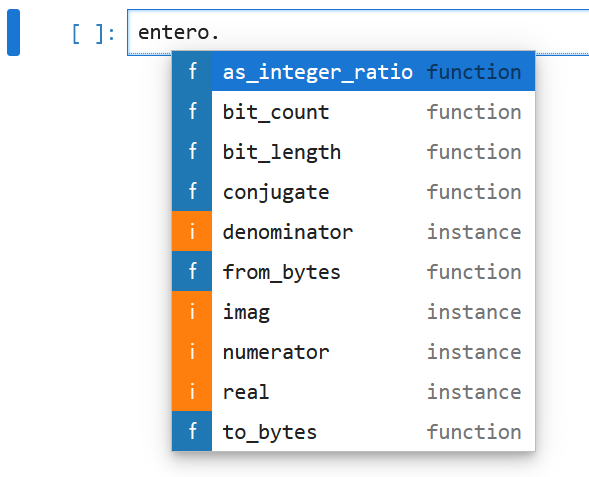
\includegraphics[width=0.4\linewidth,height=\textheight,keepaspectratio]{notebooks/../figuras/entero_python.png}

\caption{\label{fig-metodos_atributos}Métodos y atributos de los
objetos.}

\end{figure}%

Los métodos están etiquetados como \texttt{function} y los atributos
como \texttt{instance}.

En la siguiente celda realiza lo siguiente:

\begin{enumerate}
\def\labelenumi{\arabic{enumi}.}
\tightlist
\item
  Teclea \texttt{entero.} (incluye el punto al final) y luego presiona
  la tecla TAB (↹). Deberás obtener la lista de atributos y métodos como
  en la figura~\ref{fig-metodos_atributos}.
\item
  Elige el método \texttt{as\_integer\_ratio}.
\item
  Con el cursor al final de \texttt{as\_integer\_ratio} teclea SHIFT(⇧)
  + TAB(↹). Deberás obtener la documentación de los métodos como se
  muestra en la figura~\ref{fig-doc_funcion}.
\end{enumerate}

\begin{figure}

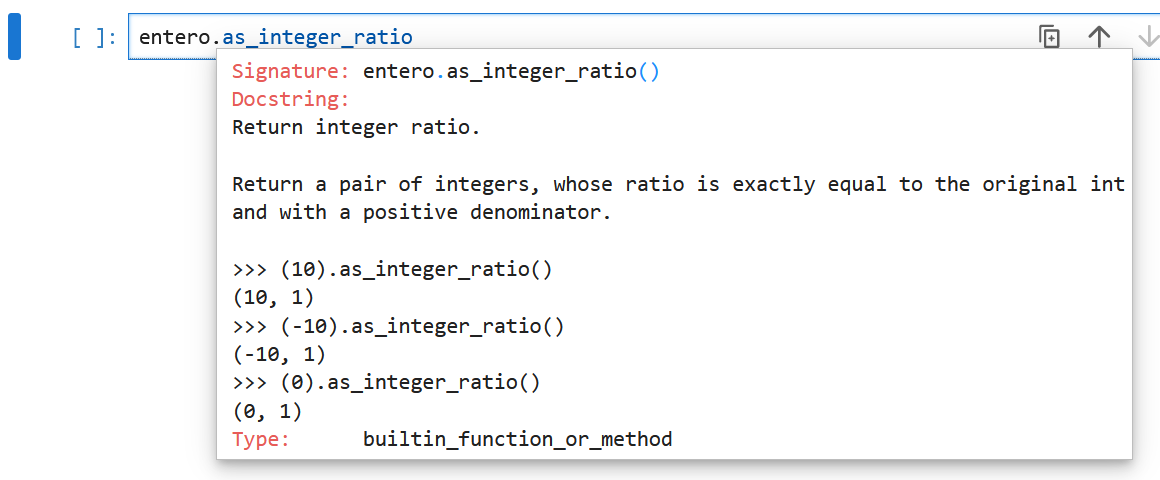
\includegraphics[width=0.8\linewidth,height=\textheight,keepaspectratio]{notebooks/../figuras/entero_python_doc.png}

\caption{\label{fig-doc_funcion}Documentación de los métodos (funciones)
de los objetos.}

\end{figure}%

Para ejecutar el método deberás primero agregar paréntesis al final del
nombre como sigue:

\begin{Shaded}
\begin{Highlighting}[]
\NormalTok{entero.as\_integer\_ratio()}
\end{Highlighting}
\end{Shaded}

\begin{verbatim}
(13, 1)
\end{verbatim}

El resultado deberá ser una pareja de enteros cuya división es
exactamente igual al número entero original. Recuerda que definimos
\texttt{entero\ =\ 13} al principio de este capítulo.

Podemos hacer exactamente lo mismo con el objeto \texttt{pi}:

\begin{Shaded}
\begin{Highlighting}[]
\NormalTok{pi.as\_integer\_ratio()}
\end{Highlighting}
\end{Shaded}

\begin{verbatim}
(3537118140137533, 1125899906842624)
\end{verbatim}

Podemos comprobar el resultado dividiendo los enteros que resultan:

\begin{Shaded}
\begin{Highlighting}[]
\DecValTok{3537118140137533} \OperatorTok{/} \DecValTok{1125899906842624}
\end{Highlighting}
\end{Shaded}

\begin{verbatim}
3.141592
\end{verbatim}

Para el caso de números complejos, vamos a elegir los atributos
\texttt{imag} y \texttt{real} que proporcionan la parte imaginaria y la
parte real del número complejo:

\begin{Shaded}
\begin{Highlighting}[]
\NormalTok{complejo.imag }\CommentTok{\# accedemos a la parte imaginaria}
\end{Highlighting}
\end{Shaded}

\begin{verbatim}
5.0
\end{verbatim}

\begin{Shaded}
\begin{Highlighting}[]
\NormalTok{complejo.real }\CommentTok{\# accedemos a la parte real}
\end{Highlighting}
\end{Shaded}

\begin{verbatim}
12.0
\end{verbatim}

Observa que en este caso no se agregaron paréntesis debido a que se
trata de atributos y no de métodos.

Finalmente, elegimos \texttt{conjugate()} y vemos el resultado:

\begin{Shaded}
\begin{Highlighting}[]
\NormalTok{complejo.conjugate() }\CommentTok{\# calculamos el conjugado del número complejo.}
\end{Highlighting}
\end{Shaded}

\begin{verbatim}
(12-5j)
\end{verbatim}

\section{Tipos lógicos}\label{tipos-luxf3gicos}

Es un tipo utilizado para realizar operaciones lógicas y puede tomar dos
valores: \texttt{True} o \texttt{False}.

\begin{Shaded}
\begin{Highlighting}[]
\NormalTok{bandera }\OperatorTok{=} \VariableTok{True}
\BuiltInTok{print}\NormalTok{(bandera, }\BuiltInTok{type}\NormalTok{(bandera))}
\end{Highlighting}
\end{Shaded}

\begin{verbatim}
True <class 'bool'>
\end{verbatim}

\begin{Shaded}
\begin{Highlighting}[]
\NormalTok{bandera }\OperatorTok{=} \VariableTok{False}
\BuiltInTok{print}\NormalTok{(bandera, }\BuiltInTok{type}\NormalTok{(bandera))}
\end{Highlighting}
\end{Shaded}

\begin{verbatim}
False <class 'bool'>
\end{verbatim}

Las variables lógicas aparecen de manera natural en operaciones
relacionales o lógicas, que se verán más adelante, por ejemplo:

¿Qué valor es mayor \(3^5\) o \(5^3\)?

Esto lo podemos preguntar como sigue:

\begin{Shaded}
\begin{Highlighting}[]
\DecValTok{3}\OperatorTok{**}\DecValTok{5} \OperatorTok{\textgreater{}} \DecValTok{5}\OperatorTok{**}\DecValTok{3}
\end{Highlighting}
\end{Shaded}

\begin{verbatim}
True
\end{verbatim}

\begin{Shaded}
\begin{Highlighting}[]
\DecValTok{3}\OperatorTok{**}\DecValTok{5} \OperatorTok{\textless{}} \DecValTok{5}\OperatorTok{**}\DecValTok{3}
\end{Highlighting}
\end{Shaded}

\begin{verbatim}
False
\end{verbatim}

Lo anterior lo podemos verificar imprimiendo los valores de \(3^5\) y
\(5^3\)

\begin{Shaded}
\begin{Highlighting}[]
\BuiltInTok{print}\NormalTok{(}\DecValTok{3}\OperatorTok{**}\DecValTok{5}\NormalTok{, }\DecValTok{5}\OperatorTok{**}\DecValTok{3}\NormalTok{)}
\end{Highlighting}
\end{Shaded}

\begin{verbatim}
243 125
\end{verbatim}

\section{\texorpdfstring{Conversión entre tipos
(\emph{casting})}{Conversión entre tipos (casting)}}\label{conversiuxf3n-entre-tipos-casting}

Es posible transformar un tipo en otro tipo compatible, a esta operación
se lo conoce como \emph{casting}.

\subsection{\texorpdfstring{Función
\texttt{int()}}{Función int()}}\label{funciuxf3n-int}

Transforma objetos en enteros, siempre y cuando haya compatibilidad.

\begin{Shaded}
\begin{Highlighting}[]
\NormalTok{cadena }\OperatorTok{=} \StringTok{\textquotesingle{}1000\textquotesingle{}}
\BuiltInTok{print}\NormalTok{(cadena, }\BuiltInTok{type}\NormalTok{(cadena))}

\NormalTok{entero }\OperatorTok{=} \BuiltInTok{int}\NormalTok{(cadena) }\CommentTok{\# Transformación}
\BuiltInTok{print}\NormalTok{(entero, }\BuiltInTok{type}\NormalTok{(entero))}
\end{Highlighting}
\end{Shaded}

\begin{verbatim}
1000 <class 'str'>
1000 <class 'int'>
\end{verbatim}

\begin{Shaded}
\begin{Highlighting}[]
\NormalTok{flotante }\OperatorTok{=} \FloatTok{3.141592}
\BuiltInTok{print}\NormalTok{(flotante, }\BuiltInTok{type}\NormalTok{(flotante))}

\NormalTok{entero  }\OperatorTok{=} \BuiltInTok{int}\NormalTok{(flotante) }\CommentTok{\# Trunca la parte decimal}
\BuiltInTok{print}\NormalTok{(entero, }\BuiltInTok{type}\NormalTok{(entero))}
\end{Highlighting}
\end{Shaded}

\begin{verbatim}
3.141592 <class 'float'>
3 <class 'int'>
\end{verbatim}

Si los objetos no son compatibles se genera un error al intentar
realizar la conversión:

\begin{Shaded}
\begin{Highlighting}[]
\NormalTok{complejo}\OperatorTok{=} \DecValTok{4}\OperatorTok{{-}}\OtherTok{4j}
\NormalTok{entero }\OperatorTok{=} \BuiltInTok{int}\NormalTok{(complejo) }\CommentTok{\# Tipos NO COMPATIBLES}
\end{Highlighting}
\end{Shaded}

\begin{Highlighting}
\textcolor{black}{TypeError: int() argument must be a string, a bytes-like object or a real number, not 'complex'}
\textcolor{black}{}\textcolor{QuartoInternalColor1}{---------------------------------------------------------------------------}\textcolor{QuartoInternalColor2}{}
\textcolor{QuartoInternalColor2}{}\textcolor{QuartoInternalColor1}{TypeError}\textcolor{QuartoInternalColor2}{                                 Traceback (most recent call last)}
\textcolor{QuartoInternalColor2}{}\textcolor{QuartoInternalColor3}{Cell}\textcolor{QuartoInternalColor2}{}\textcolor{QuartoInternalColor3}{ }\textcolor{QuartoInternalColor2}{}\textcolor{QuartoInternalColor4}{In[24]}\textcolor{QuartoInternalColor2}{}\textcolor{QuartoInternalColor4}{, line 2}\textcolor{QuartoInternalColor2}{}
\textcolor{QuartoInternalColor2}{}\textcolor{QuartoInternalColor4}{      1}\textcolor{QuartoInternalColor2}{ complejo= }\textcolor{QuartoInternalColor4}{4}\textcolor{QuartoInternalColor2}{-}\textcolor{QuartoInternalColor4}{4}\textcolor{QuartoInternalColor2}{j}
\textcolor{QuartoInternalColor2}{}\textcolor{QuartoInternalColor4}{----> }\textcolor{QuartoInternalColor2}{}\textcolor{QuartoInternalColor4}{2}\textcolor{QuartoInternalColor2}{ entero = }\textcolor{QuartoInternalColor5}{int}\textcolor{QuartoInternalColor2}{}\textcolor{QuartoInternalColor2}{(}\textcolor{QuartoInternalColor2}{}\textcolor{QuartoInternalColor2}{complejo}\textcolor{QuartoInternalColor2}{}\textcolor{QuartoInternalColor2}{)}\textcolor{QuartoInternalColor2}{ }\textcolor{QuartoInternalColor6}{# Tipos NO COMPATIBLES}\textcolor{QuartoInternalColor2}{}
\textcolor{QuartoInternalColor2}{}\textcolor{QuartoInternalColor1}{TypeError}\textcolor{QuartoInternalColor2}{: int() argument must be a string, a bytes-like object or a real number, not 'complex'}
\end{Highlighting}

Los valores lógicos \texttt{True} y \texttt{False} equivalen a
\texttt{1} y \texttt{0} respectivamente:

\begin{Shaded}
\begin{Highlighting}[]
\NormalTok{entero }\OperatorTok{=} \BuiltInTok{int}\NormalTok{(}\VariableTok{True}\NormalTok{) }
\BuiltInTok{print}\NormalTok{(entero)}
\end{Highlighting}
\end{Shaded}

\begin{verbatim}
1
\end{verbatim}

\begin{Shaded}
\begin{Highlighting}[]
\NormalTok{entero }\OperatorTok{=} \BuiltInTok{int}\NormalTok{(}\VariableTok{False}\NormalTok{) }
\BuiltInTok{print}\NormalTok{(entero)}
\end{Highlighting}
\end{Shaded}

\begin{verbatim}
0
\end{verbatim}

\subsection{\texorpdfstring{Función
\texttt{str()}}{Función str()}}\label{funciuxf3n-str}

Transforma objetos en cadenas, siempre y cuando haya compatibilidad.

\begin{Shaded}
\begin{Highlighting}[]
\NormalTok{entero }\OperatorTok{=} \DecValTok{1000}
\BuiltInTok{print}\NormalTok{(entero, }\BuiltInTok{type}\NormalTok{(entero))}

\NormalTok{cadena }\OperatorTok{=} \BuiltInTok{str}\NormalTok{(entero) }
\BuiltInTok{print}\NormalTok{(cadena, }\BuiltInTok{type}\NormalTok{(cadena))}
\end{Highlighting}
\end{Shaded}

\begin{verbatim}
1000 <class 'int'>
1000 <class 'str'>
\end{verbatim}

\begin{Shaded}
\begin{Highlighting}[]
\NormalTok{complejo }\OperatorTok{=} \DecValTok{5}\OperatorTok{+}\OtherTok{1j}
\BuiltInTok{print}\NormalTok{(complejo, }\BuiltInTok{type}\NormalTok{(complejo))}

\NormalTok{cadena }\OperatorTok{=} \BuiltInTok{str}\NormalTok{(complejo)}
\BuiltInTok{print}\NormalTok{(cadena, }\BuiltInTok{type}\NormalTok{(cadena))}
\end{Highlighting}
\end{Shaded}

\begin{verbatim}
(5+1j) <class 'complex'>
(5+1j) <class 'str'>
\end{verbatim}

\subsection{\texorpdfstring{Función
\texttt{float()}}{Función float()}}\label{funciuxf3n-float}

Transforma objetos en flotantes, siempre y cuando haya compatibilidad.

\begin{Shaded}
\begin{Highlighting}[]
\NormalTok{cadena }\OperatorTok{=} \StringTok{\textquotesingle{}3.141592\textquotesingle{}}
\BuiltInTok{print}\NormalTok{(cadena, }\BuiltInTok{type}\NormalTok{(cadena))}

\NormalTok{real }\OperatorTok{=} \BuiltInTok{float}\NormalTok{(cadena)}
\BuiltInTok{print}\NormalTok{(real, }\BuiltInTok{type}\NormalTok{(real))}
\end{Highlighting}
\end{Shaded}

\begin{verbatim}
3.141592 <class 'str'>
3.141592 <class 'float'>
\end{verbatim}

\begin{Shaded}
\begin{Highlighting}[]
\BuiltInTok{float}\NormalTok{(}\DecValTok{33}\NormalTok{)}
\end{Highlighting}
\end{Shaded}

\begin{verbatim}
33.0
\end{verbatim}

\begin{Shaded}
\begin{Highlighting}[]
\BuiltInTok{float}\NormalTok{(}\VariableTok{False}\NormalTok{)}
\end{Highlighting}
\end{Shaded}

\begin{verbatim}
0.0
\end{verbatim}

\begin{Shaded}
\begin{Highlighting}[]
\BuiltInTok{float}\NormalTok{(}\DecValTok{3}\OperatorTok{+}\OtherTok{3j}\NormalTok{) }\CommentTok{\# NO hay compatibilidad}
\end{Highlighting}
\end{Shaded}

\begin{Highlighting}
\textcolor{black}{TypeError: float() argument must be a string or a real number, not 'complex'}
\textcolor{black}{}\textcolor{QuartoInternalColor1}{---------------------------------------------------------------------------}\textcolor{QuartoInternalColor2}{}
\textcolor{QuartoInternalColor2}{}\textcolor{QuartoInternalColor1}{TypeError}\textcolor{QuartoInternalColor2}{                                 Traceback (most recent call last)}
\textcolor{QuartoInternalColor2}{}\textcolor{QuartoInternalColor3}{Cell}\textcolor{QuartoInternalColor2}{}\textcolor{QuartoInternalColor3}{ }\textcolor{QuartoInternalColor2}{}\textcolor{QuartoInternalColor4}{In[32]}\textcolor{QuartoInternalColor2}{}\textcolor{QuartoInternalColor4}{, line 1}\textcolor{QuartoInternalColor2}{}
\textcolor{QuartoInternalColor2}{}\textcolor{QuartoInternalColor4}{----> }\textcolor{QuartoInternalColor2}{}\textcolor{QuartoInternalColor4}{1}\textcolor{QuartoInternalColor2}{ }\textcolor{QuartoInternalColor5}{float}\textcolor{QuartoInternalColor2}{}\textcolor{QuartoInternalColor2}{(}\textcolor{QuartoInternalColor2}{}\textcolor{QuartoInternalColor2}{3}\textcolor{QuartoInternalColor2}{}\textcolor{QuartoInternalColor2}{+}\textcolor{QuartoInternalColor2}{}\textcolor{QuartoInternalColor2}{3}\textcolor{QuartoInternalColor2}{}\textcolor{QuartoInternalColor2}{j}\textcolor{QuartoInternalColor2}{}\textcolor{QuartoInternalColor2}{)}\textcolor{QuartoInternalColor2}{ }\textcolor{QuartoInternalColor6}{# NO hay compatibilidad}\textcolor{QuartoInternalColor2}{}
\textcolor{QuartoInternalColor2}{}\textcolor{QuartoInternalColor1}{TypeError}\textcolor{QuartoInternalColor2}{: float() argument must be a string or a real number, not 'complex'}
\end{Highlighting}

\section{\texorpdfstring{Función
\texttt{isinstance()}}{Función isinstance()}}\label{funciuxf3n-isinstance}

Permite saber si un objeto es de un tipo determinado. Por ejemplo:

\begin{Shaded}
\begin{Highlighting}[]
\NormalTok{entero }\OperatorTok{=} \DecValTok{13}
\end{Highlighting}
\end{Shaded}

\begin{Shaded}
\begin{Highlighting}[]
\BuiltInTok{print}\NormalTok{(}\BuiltInTok{isinstance}\NormalTok{(entero, }\BuiltInTok{int}\NormalTok{))}
\end{Highlighting}
\end{Shaded}

\begin{verbatim}
True
\end{verbatim}

\begin{Shaded}
\begin{Highlighting}[]
\BuiltInTok{print}\NormalTok{(}\BuiltInTok{isinstance}\NormalTok{(}\DecValTok{3}\OperatorTok{/}\DecValTok{4}\NormalTok{, }\BuiltInTok{int}\NormalTok{))}
\end{Highlighting}
\end{Shaded}

\begin{verbatim}
False
\end{verbatim}

\begin{Shaded}
\begin{Highlighting}[]
\BuiltInTok{print}\NormalTok{(}\BuiltInTok{isinstance}\NormalTok{(}\DecValTok{3}\OperatorTok{/}\DecValTok{4}\NormalTok{, }\BuiltInTok{float}\NormalTok{))}
\end{Highlighting}
\end{Shaded}

\begin{verbatim}
True
\end{verbatim}

\begin{Shaded}
\begin{Highlighting}[]
\BuiltInTok{print}\NormalTok{(}\BuiltInTok{isinstance}\NormalTok{(}\VariableTok{True}\NormalTok{, }\BuiltInTok{bool}\NormalTok{))}
\end{Highlighting}
\end{Shaded}

\begin{verbatim}
True
\end{verbatim}

\begin{Shaded}
\begin{Highlighting}[]
\BuiltInTok{print}\NormalTok{(}\BuiltInTok{isinstance}\NormalTok{(}\DecValTok{3}\OperatorTok{+}\OtherTok{5j}\NormalTok{, }\BuiltInTok{complex}\NormalTok{))}
\end{Highlighting}
\end{Shaded}

\begin{verbatim}
True
\end{verbatim}

Esta función se puede usar con cualquier tipo definido en Python o tipos
definidos por el usuario.

\section{Constantes}\label{constantes}

Python contiene una serie de constantes integradas a las que no se les
puede cambiar su valor. Más detalles se pueden encontrar en Built-in
Constants.

Las principales constantes son las siguientes:

\begin{itemize}
\item
  \texttt{False}: de tipo Booleano.
\item
  \texttt{True}: de tipo Booleano.
\item
  \texttt{None}: El único valor para el tipo \texttt{NoneType}. Es usado
  frecuentemente para representar la ausencia de un valor, por ejemplo
  cuando no se pasa un argumento a una función.
\item
  \texttt{NotImplemented}: es un valor especial que es regresado por
  métodos binarios especiales (por ejemplo \texttt{\_\_eq\_\_()},
  \texttt{\_\_lt\_\_()}, \texttt{\_\_add\_\_()},
  \texttt{\_\_rsub\_\_()}, etc.) para indicar que la operación no está
  implementada con respecto a otro tipo.
\item
  \texttt{Ellipsis}: equivalente a \texttt{...}, es un valor especial
  usado mayormente en conjunción con la sintáxis de \emph{slicing} de
  arreglos.
\item
  \texttt{\_\_debug\_\_} : Esta constante es verdadera si Python no se
  inició con la opción \texttt{-O}.
\end{itemize}

Las siguientes constantes son usadas dentro del intérprete interactivo
(no se pueden usar dentro de programas ejecutados fuera del intérprete).

\begin{itemize}
\tightlist
\item
  \texttt{quit}(code=None)
\item
  \texttt{exit}(code=None)
\item
  \texttt{copyright}
\item
  \texttt{credits}
\item
  \texttt{license}
\end{itemize}

Por ejemplo:

\begin{Shaded}
\begin{Highlighting}[]
\NormalTok{copyright()}
\end{Highlighting}
\end{Shaded}

\begin{verbatim}
Copyright (c) 2001-2024 Python Software Foundation.
All Rights Reserved.

Copyright (c) 2000 BeOpen.com.
All Rights Reserved.

Copyright (c) 1995-2001 Corporation for National Research Initiatives.
All Rights Reserved.

Copyright (c) 1991-1995 Stichting Mathematisch Centrum, Amsterdam.
All Rights Reserved.
\end{verbatim}

\begin{Shaded}
\begin{Highlighting}[]
\NormalTok{credits()}
\end{Highlighting}
\end{Shaded}

\begin{verbatim}
    Thanks to CWI, CNRI, BeOpen, Zope Corporation, the Python Software
    Foundation, and a cast of thousands for supporting Python
    development.  See www.python.org for more information.
\end{verbatim}

\bookmarksetup{startatroot}

\chapter{Operadores.}\label{operadores.}

\textbf{Objetivo.} Explicar los operadores aritméticos, relacionales y
lógicos, así como mostrar su uso con varios ejemplos.

\section{Operadores aritméticos}\label{operadores-aritmuxe9ticos}

Para los tipos numéricos básicos, existen operaciones aritméticas que se
pueden aplicar sobre ellos. Estas operaciones están organizadas como se
muestra en la siguiente tabla:

\begin{longtable}[]{@{}ll@{}}
\toprule\noalign{}
Categoría & Operadores \\
\midrule\noalign{}
\endhead
\bottomrule\noalign{}
\endlastfoot
Exponenciación & \texttt{**} \\
Multiplicación & \texttt{*},\texttt{/},\texttt{//},\texttt{\%} \\
Adición & \texttt{+},\texttt{-} \\
\end{longtable}

Veamos algunos ejemplos:

\begin{Shaded}
\begin{Highlighting}[]
\CommentTok{\# Suma}
\NormalTok{suma }\OperatorTok{=} \DecValTok{1} \OperatorTok{+} \DecValTok{2}

\CommentTok{\# Imprimimos el resultado y el tipo}
\BuiltInTok{print}\NormalTok{(suma, }\BuiltInTok{type}\NormalTok{(suma))}
\end{Highlighting}
\end{Shaded}

\begin{verbatim}
3 <class 'int'>
\end{verbatim}

\begin{Shaded}
\begin{Highlighting}[]
\CommentTok{\# Resta}
\NormalTok{resta }\OperatorTok{=} \DecValTok{5} \OperatorTok{{-}} \DecValTok{32}

\CommentTok{\# Imprimimos el resultado y el tipo}
\BuiltInTok{print}\NormalTok{(resta, }\BuiltInTok{type}\NormalTok{(resta))}
\end{Highlighting}
\end{Shaded}

\begin{verbatim}
-27 <class 'int'>
\end{verbatim}

\begin{Shaded}
\begin{Highlighting}[]
\CommentTok{\# Multiplicación}
\NormalTok{multiplicacion }\OperatorTok{=} \DecValTok{3} \OperatorTok{*} \DecValTok{3}

\CommentTok{\# Imprimimos el resultado y el tipo}
\BuiltInTok{print}\NormalTok{(multiplicacion, }\BuiltInTok{type}\NormalTok{(multiplicacion))}
\end{Highlighting}
\end{Shaded}

\begin{verbatim}
9 <class 'int'>
\end{verbatim}

\begin{Shaded}
\begin{Highlighting}[]
\CommentTok{\# División}
\NormalTok{division }\OperatorTok{=} \DecValTok{3} \OperatorTok{/} \DecValTok{2}

\CommentTok{\# Imprimimos el resultado y el tipo}
\BuiltInTok{print}\NormalTok{(division, }\BuiltInTok{type}\NormalTok{(division))}
\end{Highlighting}
\end{Shaded}

\begin{verbatim}
1.5 <class 'float'>
\end{verbatim}

\begin{Shaded}
\begin{Highlighting}[]
\CommentTok{\# División entera: divide los números y elimina la parte decimal}
\NormalTok{div\_entera }\OperatorTok{=} \DecValTok{50} \OperatorTok{//} \DecValTok{3}

\CommentTok{\# Imprimimos el resultado y el tipo}
\BuiltInTok{print}\NormalTok{(div\_entera, }\BuiltInTok{type}\NormalTok{(div\_entera))}
\end{Highlighting}
\end{Shaded}

\begin{verbatim}
16 <class 'int'>
\end{verbatim}

\begin{Shaded}
\begin{Highlighting}[]
\CommentTok{\# Módulo: divide los números y regresa el residuo.}
\NormalTok{modulo }\OperatorTok{=} \DecValTok{50} \OperatorTok{\%} \DecValTok{3}

\CommentTok{\# Imprimimos el resultado y el tipo}
\BuiltInTok{print}\NormalTok{(modulo, }\BuiltInTok{type}\NormalTok{(modulo))}
\end{Highlighting}
\end{Shaded}

\begin{verbatim}
2 <class 'int'>
\end{verbatim}

\begin{Shaded}
\begin{Highlighting}[]
\CommentTok{\# Potencia usando un entero}
\NormalTok{potencia }\OperatorTok{=} \DecValTok{9}\OperatorTok{**}\DecValTok{2} \CommentTok{\# 9 al cuadrado}

\CommentTok{\# Imprimimos el resultado y el tipo}
\BuiltInTok{print}\NormalTok{(potencia, }\BuiltInTok{type}\NormalTok{(potencia))}
\end{Highlighting}
\end{Shaded}

\begin{verbatim}
81 <class 'int'>
\end{verbatim}

\begin{Shaded}
\begin{Highlighting}[]
\CommentTok{\# Potencia usando un número decimal}
\NormalTok{potencia }\OperatorTok{=} \DecValTok{81}\OperatorTok{**}\FloatTok{0.5} \CommentTok{\# raíz cuadrada de 81}

\CommentTok{\# Imprimimos el resultado y el tipo}
\BuiltInTok{print}\NormalTok{(potencia, }\BuiltInTok{type}\NormalTok{(potencia))}
\end{Highlighting}
\end{Shaded}

\begin{verbatim}
9.0 <class 'float'>
\end{verbatim}

\begin{Shaded}
\begin{Highlighting}[]
\CommentTok{\# Potencia usando un número decimal}
\NormalTok{potencia }\OperatorTok{=} \DecValTok{2}\OperatorTok{**}\NormalTok{(}\FloatTok{0.35}\NormalTok{) }\CommentTok{\# 2 elevado a la potencia 0.35}

\CommentTok{\# Imprimimos el resultado y el tipo}
\BuiltInTok{print}\NormalTok{(potencia, }\BuiltInTok{type}\NormalTok{(potencia))}
\end{Highlighting}
\end{Shaded}

\begin{verbatim}
1.2745606273192622 <class 'float'>
\end{verbatim}

\section{Precedencia.}\label{sec-precedencia}

La aplicación de los operadores tiene cierta precedencia que está
definida en cada implementación del lenguaje de programación. La
siguiente tabla muestra el orden en que se aplicarán los operadores.

\begin{longtable}[]{@{}lll@{}}
\toprule\noalign{}
Nivel & Categoría & Operadores \\
\midrule\noalign{}
\endhead
\bottomrule\noalign{}
\endlastfoot
7 & exponenciación & \texttt{**} \\
6 & multiplicación & \texttt{*},\texttt{/},\texttt{//},\texttt{\%} \\
5 & adición & \texttt{+},\texttt{-} \\
4 & relacional &
\texttt{==},\texttt{!=},\texttt{\textless{}=},\texttt{\textgreater{}=},\texttt{\textgreater{}},\texttt{\textless{}} \\
3 & lógicos & \texttt{not} \\
2 & lógicos & \texttt{and} \\
1 & lógicos & \texttt{or} \\
\end{longtable}

Como se puede ver, siempre se aplican primero los operadores aritméticos
(niveles 7, 6, y 5), luego los relacionales (nivel 4) y finalmente los
lógicos (3, 2 y 1).

Más acerca de este tema se puede ver aquí: Operator precedence.

A continuación se muestran ejemplos de operaciones aritméticas en donde
se resalta esta precedencia:

\begin{Shaded}
\begin{Highlighting}[]
\CommentTok{\# Precedencia de operaciones: primero se realiza la multiplicación}
\DecValTok{1} \OperatorTok{+} \DecValTok{2} \OperatorTok{*} \DecValTok{3} \OperatorTok{+} \DecValTok{4}
\end{Highlighting}
\end{Shaded}

\begin{verbatim}
11
\end{verbatim}

\begin{Shaded}
\begin{Highlighting}[]
\CommentTok{\# Es posible usar paréntesis para modificar la precedencia: primero la suma}
\NormalTok{(}\DecValTok{1} \OperatorTok{+} \DecValTok{2}\NormalTok{) }\OperatorTok{*}\NormalTok{ (}\DecValTok{3} \OperatorTok{+} \DecValTok{4}\NormalTok{)}
\end{Highlighting}
\end{Shaded}

\begin{verbatim}
21
\end{verbatim}

\begin{Shaded}
\begin{Highlighting}[]
\CommentTok{\# Primero se realiza la exponenciación}
\DecValTok{3}\OperatorTok{**}\DecValTok{2}\OperatorTok{/}\DecValTok{2}
\end{Highlighting}
\end{Shaded}

\begin{verbatim}
4.5
\end{verbatim}

\section{Operaciones entre tipos
diferentes}\label{operaciones-entre-tipos-diferentes}

Es posible combinar operaciones entre tipos de números diferentes. Lo
que Python hará es promover cada número al tipo más sofisticado, siendo
el orden de sofisticación, de menos a más, como sigue: \texttt{int},
\texttt{float}, \texttt{complex}.

\begin{Shaded}
\begin{Highlighting}[]
\CommentTok{\# Operación entre enteros}
\NormalTok{a }\OperatorTok{=} \DecValTok{2} \OperatorTok{*} \DecValTok{3}
\BuiltInTok{print}\NormalTok{(a, }\BuiltInTok{type}\NormalTok{(a))}
\end{Highlighting}
\end{Shaded}

\begin{verbatim}
6 <class 'int'>
\end{verbatim}

\begin{Shaded}
\begin{Highlighting}[]
\CommentTok{\# Operación entre entero y flotante}
\NormalTok{a }\OperatorTok{=} \DecValTok{2} \OperatorTok{*} \FloatTok{3.0}
\BuiltInTok{print}\NormalTok{(a, }\BuiltInTok{type}\NormalTok{(a))}
\end{Highlighting}
\end{Shaded}

\begin{verbatim}
6.0 <class 'float'>
\end{verbatim}

\begin{Shaded}
\begin{Highlighting}[]
\CommentTok{\# Operación entre entero y complejo}
\NormalTok{a }\OperatorTok{=} \DecValTok{2} \OperatorTok{*}\NormalTok{ (}\DecValTok{1} \OperatorTok{+} \OtherTok{3j}\NormalTok{)}
\BuiltInTok{print}\NormalTok{(a, }\BuiltInTok{type}\NormalTok{(a))}
\end{Highlighting}
\end{Shaded}

\begin{verbatim}
(2+6j) <class 'complex'>
\end{verbatim}

\begin{Shaded}
\begin{Highlighting}[]
\CommentTok{\# Operación entre flotante y complejo}
\NormalTok{a }\OperatorTok{=} \FloatTok{2.0} \OperatorTok{*}\NormalTok{ (}\DecValTok{1} \OperatorTok{+} \OtherTok{3j}\NormalTok{)}
\BuiltInTok{print}\NormalTok{(a, }\BuiltInTok{type}\NormalTok{(a))}
\end{Highlighting}
\end{Shaded}

\begin{verbatim}
(2+6j) <class 'complex'>
\end{verbatim}

\begin{Shaded}
\begin{Highlighting}[]
\CommentTok{\# División entre enteros que da como resultado un flotante}
\NormalTok{a }\OperatorTok{=} \DecValTok{2}\OperatorTok{/}\DecValTok{3}
\BuiltInTok{print}\NormalTok{(a, }\BuiltInTok{type}\NormalTok{(a))}
\end{Highlighting}
\end{Shaded}

\begin{verbatim}
0.6666666666666666 <class 'float'>
\end{verbatim}

\section{Operadores de asignación}\label{operadores-de-asignaciuxf3n}

Existen varios operadores para realizar asignaciones:

\begin{longtable}[]{@{}lll@{}}
\toprule\noalign{}
Operador & Operación & Equivalencia \\
\midrule\noalign{}
\endhead
\bottomrule\noalign{}
\endlastfoot
\texttt{+=} & \texttt{b\ +=\ a} & \texttt{b\ =\ b\ +\ a} \\
\texttt{-=} & \texttt{b\ -=\ a} & \texttt{b\ =\ b\ -\ a} \\
\texttt{*=} & \texttt{b\ *=\ a} & \texttt{b\ =\ b\ *\ a} \\
\texttt{/=} & \texttt{b\ /=\ a} & \texttt{b\ =\ b\ /\ a} \\
\texttt{//=} & \texttt{b\ //=\ a} & \texttt{b\ =\ b\ //\ a} \\
\texttt{\%=} & \texttt{b\ \%=\ a} & \texttt{b\ =\ b\ \%\ a} \\
\texttt{**=} & \texttt{b\ **=\ a} & \texttt{b\ =\ b\ **\ a} \\
\end{longtable}

La forma de uso de estos operadores se muestra en los siguientes
ejemplos:

\begin{Shaded}
\begin{Highlighting}[]
\NormalTok{a }\OperatorTok{=} \FloatTok{1.0} 
\NormalTok{b }\OperatorTok{=} \FloatTok{1.0}
\NormalTok{b }\OperatorTok{+=}\NormalTok{ a  }
\BuiltInTok{print}\NormalTok{(b)}
\end{Highlighting}
\end{Shaded}

\begin{verbatim}
2.0
\end{verbatim}

\begin{Shaded}
\begin{Highlighting}[]
\NormalTok{a }\OperatorTok{=}  \DecValTok{4}
\NormalTok{b }\OperatorTok{=} \DecValTok{16}
\NormalTok{b }\OperatorTok{{-}=}\NormalTok{ a  }
\BuiltInTok{print}\NormalTok{(b)}
\end{Highlighting}
\end{Shaded}

\begin{verbatim}
12
\end{verbatim}

\begin{Shaded}
\begin{Highlighting}[]
\NormalTok{a }\OperatorTok{=} \DecValTok{2}
\NormalTok{b }\OperatorTok{=} \DecValTok{12}
\NormalTok{b }\OperatorTok{*=}\NormalTok{ a  }
\BuiltInTok{print}\NormalTok{(b)}
\end{Highlighting}
\end{Shaded}

\begin{verbatim}
24
\end{verbatim}

\begin{Shaded}
\begin{Highlighting}[]
\NormalTok{a }\OperatorTok{=} \DecValTok{3}
\NormalTok{b }\OperatorTok{=} \DecValTok{50}
\NormalTok{b }\OperatorTok{/=}\NormalTok{ a }
\BuiltInTok{print}\NormalTok{(b)}
\end{Highlighting}
\end{Shaded}

\begin{verbatim}
16.666666666666668
\end{verbatim}

\begin{Shaded}
\begin{Highlighting}[]
\NormalTok{a }\OperatorTok{=} \DecValTok{3}
\NormalTok{b }\OperatorTok{=} \DecValTok{50}
\NormalTok{b }\OperatorTok{//=}\NormalTok{ a }
\BuiltInTok{print}\NormalTok{(b)}
\end{Highlighting}
\end{Shaded}

\begin{verbatim}
16
\end{verbatim}

\begin{Shaded}
\begin{Highlighting}[]
\NormalTok{a }\OperatorTok{=} \DecValTok{3}
\NormalTok{b }\OperatorTok{=} \DecValTok{50}
\NormalTok{b }\OperatorTok{\%=}\NormalTok{ a}
\BuiltInTok{print}\NormalTok{(b)}
\end{Highlighting}
\end{Shaded}

\begin{verbatim}
2
\end{verbatim}

\begin{Shaded}
\begin{Highlighting}[]
\NormalTok{a }\OperatorTok{=} \DecValTok{2}
\NormalTok{b }\OperatorTok{=} \DecValTok{3}
\NormalTok{b }\OperatorTok{**=}\NormalTok{ a }
\BuiltInTok{print}\NormalTok{(b)}
\end{Highlighting}
\end{Shaded}

\begin{verbatim}
9
\end{verbatim}

\section{Operadores relacionales}\label{operadores-relacionales}

Cuando se aplica un operador relacional a dos expresiones, se realiza
una comparación entre dichas expresiones y se obtiene como resultado un
tipo lógico (\texttt{bool}): \texttt{True} o \texttt{False}.

Los operadores relacionales que están definidos son:

\begin{longtable}[]{@{}lll@{}}
\toprule\noalign{}
Operador & Operación & Significado \\
\midrule\noalign{}
\endhead
\bottomrule\noalign{}
\endlastfoot
\texttt{==} & \texttt{A\ ==\ B} & ¿Es \texttt{A} igual a \texttt{B}? \\
\texttt{!=} & \texttt{A\ !=\ B} & ¿Es \texttt{A} diferente de
\texttt{B}? \\
\texttt{\textgreater{}} & \texttt{A\ \textgreater{}\ B} & ¿Es \texttt{A}
mayor que \texttt{B}? \\
\texttt{\textgreater{}=} & \texttt{A\ \textgreater{}=\ B} & ¿Es
\texttt{A} mayor o igual a \texttt{B}? \\
\texttt{\textgreater{}} & \texttt{A\ \textless{}\ B} & ¿Es \texttt{A}
menor que \texttt{B}? \\
\texttt{\textless{}=} & \texttt{A\ \textgreater{}=\ B} & ¿Es \texttt{A}
menor o igual a \texttt{B}? \\
\end{longtable}

A continuación se muestran algunos ejemplos:

\begin{Shaded}
\begin{Highlighting}[]
\CommentTok{\# ¿Es 35 mayor que 562?}
\DecValTok{35} \OperatorTok{\textgreater{}} \DecValTok{562} 
\end{Highlighting}
\end{Shaded}

\begin{verbatim}
False
\end{verbatim}

\begin{Shaded}
\begin{Highlighting}[]
\CommentTok{\# ¿Es 32 mayor o igual que 21?}
\DecValTok{32} \OperatorTok{\textgreater{}=} \DecValTok{21} 
\end{Highlighting}
\end{Shaded}

\begin{verbatim}
True
\end{verbatim}

\begin{Shaded}
\begin{Highlighting}[]
\CommentTok{\# ¿Es 12 menor que 34?}
\DecValTok{12} \OperatorTok{\textless{}} \DecValTok{34} 
\end{Highlighting}
\end{Shaded}

\begin{verbatim}
True
\end{verbatim}

\begin{Shaded}
\begin{Highlighting}[]
\CommentTok{\# ¿Es 12 menor o igual que 25?}
\DecValTok{12} \OperatorTok{\textless{}=} \DecValTok{25} 
\end{Highlighting}
\end{Shaded}

\begin{verbatim}
True
\end{verbatim}

\begin{Shaded}
\begin{Highlighting}[]
\CommentTok{\# ¿Es 1 igual a 2?}
\DecValTok{1} \OperatorTok{==} \DecValTok{2} 
\end{Highlighting}
\end{Shaded}

\begin{verbatim}
False
\end{verbatim}

\begin{Shaded}
\begin{Highlighting}[]
\CommentTok{\# ¿Es 1 diferente de 2?}
\DecValTok{1} \OperatorTok{!=} \DecValTok{2}
\end{Highlighting}
\end{Shaded}

\begin{verbatim}
True
\end{verbatim}

\begin{Shaded}
\begin{Highlighting}[]
\CommentTok{\# Se pueden comparar otros tipos de datos}
\CommentTok{\textquotesingle{}aaa\textquotesingle{}} \OperatorTok{==} \StringTok{\textquotesingle{}aaaA\textquotesingle{}} 
\end{Highlighting}
\end{Shaded}

\begin{verbatim}
False
\end{verbatim}

\begin{Shaded}
\begin{Highlighting}[]
\CommentTok{\# La comparación se puede hacer con el resultado de expresiones}
\DecValTok{5} \OperatorTok{\textgreater{}} \BuiltInTok{len}\NormalTok{(}\StringTok{\textquotesingle{}5\textquotesingle{}}\NormalTok{)}
\end{Highlighting}
\end{Shaded}

\begin{verbatim}
True
\end{verbatim}

\section{Operaciones lógicas.}\label{operaciones-luxf3gicas.}

Los operadores lógicos que se pueden usar son:

\begin{longtable}[]{@{}
  >{\raggedright\arraybackslash}p{(\linewidth - 4\tabcolsep) * \real{0.3333}}
  >{\raggedright\arraybackslash}p{(\linewidth - 4\tabcolsep) * \real{0.3333}}
  >{\raggedright\arraybackslash}p{(\linewidth - 4\tabcolsep) * \real{0.3333}}@{}}
\toprule\noalign{}
\begin{minipage}[b]{\linewidth}\raggedright
Operador
\end{minipage} & \begin{minipage}[b]{\linewidth}\raggedright
Uso
\end{minipage} & \begin{minipage}[b]{\linewidth}\raggedright
Resultado
\end{minipage} \\
\midrule\noalign{}
\endhead
\bottomrule\noalign{}
\endlastfoot
\texttt{not} & \texttt{not\ A} & Invierte el resultado de \texttt{A} \\
\texttt{and} & \texttt{A\ and\ B} & \texttt{True} si \texttt{A} y
\texttt{B} son \texttt{True}; \texttt{False} en otro caso \\
\texttt{or} & \texttt{A\ or\ B} & \texttt{False} si \texttt{A} y
\texttt{B} son \texttt{False}; \texttt{True} en otro caso \\
\end{longtable}

Veamos algunos ejemplos.

\subsection{\texorpdfstring{\texttt{and}}{and}}\label{and}

Para que el resultado sea verdadero, se deben cumplir las dos
expresiones que se encuentran a la derecha e izquierda del \texttt{and}.
Si una de ellas no se cumple, el resultado será falso.

\begin{Shaded}
\begin{Highlighting}[]
\NormalTok{(}\DecValTok{5} \OperatorTok{\textless{}} \DecValTok{32}\NormalTok{) }\KeywordTok{and}\NormalTok{ (}\DecValTok{63} \OperatorTok{\textgreater{}} \DecValTok{32}\NormalTok{) }
\end{Highlighting}
\end{Shaded}

\begin{verbatim}
True
\end{verbatim}

Debido a la precedencia de operadores (véase
Sección~\ref{sec-precedencia}), no son necesarios los paréntesis en la
operaciones relacionales de la expresión anterior, por lo que es posible
escribir:

\begin{Shaded}
\begin{Highlighting}[]
\DecValTok{5} \OperatorTok{\textless{}} \DecValTok{32} \KeywordTok{and} \DecValTok{63} \OperatorTok{\textgreater{}} \DecValTok{32}
\end{Highlighting}
\end{Shaded}

\begin{verbatim}
True
\end{verbatim}

Aunque a veces el uso de paréntesis hace la lectura del código más
clara:

\begin{Shaded}
\begin{Highlighting}[]
\NormalTok{(}\FloatTok{2.32} \OperatorTok{\textless{}} \DecValTok{21}\NormalTok{) }\KeywordTok{and}\NormalTok{ (}\DecValTok{23} \OperatorTok{\textgreater{}} \DecValTok{63}\NormalTok{)}
\end{Highlighting}
\end{Shaded}

\begin{verbatim}
False
\end{verbatim}

\subsection{\texorpdfstring{\texttt{or}}{or}}\label{or}

Para que el resultado sea verdadero, se deben cumplir una de las dos
expresiones que se encuentran a la derecha e izquierda del `or'. Si una
de ellas se cumple, el resultado será verdadero.

\begin{Shaded}
\begin{Highlighting}[]
\NormalTok{(}\DecValTok{32} \OperatorTok{==} \DecValTok{21}\NormalTok{) }\KeywordTok{or}\NormalTok{ (}\DecValTok{5} \OperatorTok{\textless{}} \DecValTok{31}\NormalTok{)}
\end{Highlighting}
\end{Shaded}

\begin{verbatim}
True
\end{verbatim}

Para que el resultado sea falso, ambas expresiones deben ser falsas.

\begin{Shaded}
\begin{Highlighting}[]
\NormalTok{(}\DecValTok{32} \OperatorTok{==} \DecValTok{21}\NormalTok{) }\KeywordTok{or}\NormalTok{ (}\DecValTok{31} \OperatorTok{\textless{}} \DecValTok{5}\NormalTok{) }
\end{Highlighting}
\end{Shaded}

\begin{verbatim}
False
\end{verbatim}

\subsection{\texorpdfstring{\texttt{not}}{not}}\label{not}

Este operador es usado para obtener el valor Booleano opuesto al valor
actual de una variable. Se conoce como el operador de \emph{negación}.

\begin{Shaded}
\begin{Highlighting}[]
\CommentTok{\# Invierte el resultado de la expresión}
\KeywordTok{not} \VariableTok{True}
\end{Highlighting}
\end{Shaded}

\begin{verbatim}
False
\end{verbatim}

\begin{Shaded}
\begin{Highlighting}[]
\NormalTok{a }\OperatorTok{=} \DecValTok{32} \OperatorTok{!=} \DecValTok{32}
\BuiltInTok{print}\NormalTok{(a)}
\BuiltInTok{print}\NormalTok{(}\KeywordTok{not}\NormalTok{ a)}
\end{Highlighting}
\end{Shaded}

\begin{verbatim}
False
True
\end{verbatim}

\section{\texorpdfstring{Operador
\texttt{is}}{Operador is}}\label{operador-is}

Este operador permite comprobar si dos objetos son el mismo. Por
ejemplo:

\begin{Shaded}
\begin{Highlighting}[]
\NormalTok{a }\OperatorTok{=} \DecValTok{1}
\NormalTok{b }\OperatorTok{=}\NormalTok{ a}

\CommentTok{\# Preguntamos si \textquotesingle{}b\textquotesingle{} representa el mismo objeto que \textquotesingle{}a\textquotesingle{}}
\BuiltInTok{print}\NormalTok{(}\StringTok{\textquotesingle{}¿b es a?\textquotesingle{}}\NormalTok{, b }\KeywordTok{is}\NormalTok{ a)}

\CommentTok{\# Imprimimos sus identificadores en memoria}
\BuiltInTok{print}\NormalTok{(}\StringTok{\textquotesingle{}id(a) = \textquotesingle{}}\NormalTok{, }\BuiltInTok{id}\NormalTok{(a))}
\BuiltInTok{print}\NormalTok{(}\StringTok{\textquotesingle{}id(b) = \textquotesingle{}}\NormalTok{, }\BuiltInTok{id}\NormalTok{(b))}
\end{Highlighting}
\end{Shaded}

\begin{verbatim}
¿b es a? True
id(a) =  140714900202408
id(b) =  140714900202408
\end{verbatim}

Podemos hacer la pregunta inversa agregando el operador \texttt{not}:

\begin{Shaded}
\begin{Highlighting}[]
\CommentTok{\# Preguntamos si \textquotesingle{}b\textquotesingle{} NO representa el mismo objeto que \textquotesingle{}a\textquotesingle{}}
\BuiltInTok{print}\NormalTok{(}\StringTok{\textquotesingle{}¿b NO es a?\textquotesingle{}}\NormalTok{, b }\KeywordTok{is} \KeywordTok{not}\NormalTok{ a)}

\CommentTok{\# Imprimimos sus identificadores en memoria}
\BuiltInTok{print}\NormalTok{(}\StringTok{\textquotesingle{}id(a) = \textquotesingle{}}\NormalTok{, }\BuiltInTok{id}\NormalTok{(a))}
\BuiltInTok{print}\NormalTok{(}\StringTok{\textquotesingle{}id(b) = \textquotesingle{}}\NormalTok{, }\BuiltInTok{id}\NormalTok{(b))}
\end{Highlighting}
\end{Shaded}

\begin{verbatim}
¿b NO es a? False
id(a) =  140714900202408
id(b) =  140714900202408
\end{verbatim}

Finalmente, si modificamos \texttt{b} tenemos:

\begin{Shaded}
\begin{Highlighting}[]
\NormalTok{b }\OperatorTok{=} \FloatTok{5.0}
\BuiltInTok{print}\NormalTok{(}\StringTok{\textquotesingle{}¿b es a?\textquotesingle{}}\NormalTok{, b }\KeywordTok{is}\NormalTok{ a)}
\BuiltInTok{print}\NormalTok{(}\StringTok{\textquotesingle{}¿b NO es a?\textquotesingle{}}\NormalTok{, b }\KeywordTok{is} \KeywordTok{not}\NormalTok{ a)}
\BuiltInTok{print}\NormalTok{(}\StringTok{\textquotesingle{}id(a) = \textquotesingle{}}\NormalTok{, }\BuiltInTok{id}\NormalTok{(a))}
\BuiltInTok{print}\NormalTok{(}\StringTok{\textquotesingle{}id(b) = \textquotesingle{}}\NormalTok{, }\BuiltInTok{id}\NormalTok{(b))}
\end{Highlighting}
\end{Shaded}

\begin{verbatim}
¿b es a? False
¿b NO es a? True
id(a) =  140714900202408
id(b) =  2288439605360
\end{verbatim}

\section{Comparación entre números
flotantes.}\label{comparaciuxf3n-entre-nuxfameros-flotantes.}

La comparación entre números de tipo flotante debe realizarse con
cuidado, veamos el siguiente ejemplo:

\begin{Shaded}
\begin{Highlighting}[]
\NormalTok{(}\FloatTok{0.4} \OperatorTok{{-}} \FloatTok{0.3}\NormalTok{) }\OperatorTok{==} \FloatTok{0.1}
\end{Highlighting}
\end{Shaded}

\begin{verbatim}
False
\end{verbatim}

El cálculo a mano de \texttt{(0.4\ -\ 0.3)} da como resultado
\texttt{0.1}, pero en una computadora este cálculo es aproximado y
depende de las características del hardware (exponente, mantisa, base,
etcétera), véase Floating-Point Arithmetic para más información.

En Python el resultado de la operación \texttt{(0.4\ -\ 0.3)} es
diferente de \texttt{0.1}, veamos:

\begin{Shaded}
\begin{Highlighting}[]
\BuiltInTok{print}\NormalTok{(}\FloatTok{0.4} \OperatorTok{{-}} \FloatTok{0.3}\NormalTok{)}
\end{Highlighting}
\end{Shaded}

\begin{verbatim}
0.10000000000000003
\end{verbatim}

Python ofrece herramientas que permiten realizar una mejor comparación
entre números de tipo flotante. Por ejemplo la biblioteca \texttt{math}
contiene la función \texttt{isclose(a,\ b)} en donde se puede definir
una tolerancia mínima para que las dos expresiones, \texttt{a} y
\texttt{b} se consideren iguales (\emph{cercanas}), por ejemplo:

\begin{Shaded}
\begin{Highlighting}[]
\CommentTok{\# Importamos el módulo math}
\ImportTok{import}\NormalTok{ math}

\CommentTok{\# Utilizamos la función \textasciigrave{}isclose()\textasciigrave{} de math para comparar dos números flotantes}
\NormalTok{math.isclose((}\FloatTok{0.4} \OperatorTok{{-}} \FloatTok{0.3}\NormalTok{), }\FloatTok{0.1}\NormalTok{)}
\end{Highlighting}
\end{Shaded}

\begin{verbatim}
True
\end{verbatim}

Se recomienda revisar el manual de \texttt{math.isclose()} y el de
\texttt{numpy.isclose()} para comparación de arreglos con elementos de
tipo flotante.

\section{Fuertemente tipado.}\label{fuertemente-tipado.}

Python es fuertemente tipado, lo que significa que el tipo de un objeto
no puede cambiar repentinamente, se debe realizar una conversión
explícita si se desea cambiar el tipo de un objeto.

Esta característica también impide que se realizen operaciones entre
tipos no compatibles.

Veamos unos ejemplos:

\begin{Shaded}
\begin{Highlighting}[]
\CommentTok{\# Definimos tres números}
\NormalTok{real   }\OperatorTok{=} \FloatTok{220.0}  
\NormalTok{entero }\OperatorTok{=} \DecValTok{284}
\NormalTok{complejo }\OperatorTok{=} \DecValTok{1}\OperatorTok{+}\OtherTok{1j}
\end{Highlighting}
\end{Shaded}

\begin{Shaded}
\begin{Highlighting}[]
\NormalTok{entero }\OperatorTok{+}\NormalTok{ real }\CommentTok{\# Los tipos son compatibles}
\end{Highlighting}
\end{Shaded}

\begin{verbatim}
504.0
\end{verbatim}

\begin{Shaded}
\begin{Highlighting}[]
\NormalTok{real }\OperatorTok{+}\NormalTok{ complejo }\CommentTok{\# Los tipos son compatibles}
\end{Highlighting}
\end{Shaded}

\begin{verbatim}
(221+1j)
\end{verbatim}

\begin{Shaded}
\begin{Highlighting}[]
\NormalTok{entero }\OperatorTok{+}\NormalTok{ complejo }\CommentTok{\# Los tipos son compatibles}
\end{Highlighting}
\end{Shaded}

\begin{verbatim}
(285+1j)
\end{verbatim}

Un tipo lógico se puede comportar como un entero, un flotante o un
complejo, los tipos son compatibles. Para que un valor numérico sea
considerado verdadero, debe ser equivalente a \texttt{1}.

Veamos los siguientes ejemplos:

\begin{Shaded}
\begin{Highlighting}[]
\NormalTok{lógico }\OperatorTok{=} \VariableTok{True} 
\BuiltInTok{print}\NormalTok{(lógico }\OperatorTok{==} \DecValTok{1}\NormalTok{)}
\BuiltInTok{print}\NormalTok{(lógico }\OperatorTok{==} \FloatTok{1.0}\NormalTok{)}
\BuiltInTok{print}\NormalTok{(lógico }\OperatorTok{==} \FloatTok{1.0} \OperatorTok{+} \OtherTok{0.0j}\NormalTok{)}
\end{Highlighting}
\end{Shaded}

\begin{verbatim}
True
True
True
\end{verbatim}

\begin{Shaded}
\begin{Highlighting}[]
\BuiltInTok{print}\NormalTok{(lógico }\OperatorTok{==} \DecValTok{5}\NormalTok{)}
\BuiltInTok{print}\NormalTok{(lógico }\OperatorTok{==} \FloatTok{1.1}\NormalTok{)}
\BuiltInTok{print}\NormalTok{(lógico }\OperatorTok{==} \FloatTok{1.0} \OperatorTok{+} \OtherTok{0.1j}\NormalTok{)}
\end{Highlighting}
\end{Shaded}

\begin{verbatim}
False
False
False
\end{verbatim}

Entonces podemos realizar operaciones aritméticas entre lógicos,
enteros, flotantes y complejos:

\begin{Shaded}
\begin{Highlighting}[]
\NormalTok{lógico }\OperatorTok{+}\NormalTok{ entero }\CommentTok{\# Los tipos son compatibles}
\end{Highlighting}
\end{Shaded}

\begin{verbatim}
285
\end{verbatim}

\begin{Shaded}
\begin{Highlighting}[]
\NormalTok{lógico }\OperatorTok{+}\NormalTok{ real }\CommentTok{\# Los tipos son compatibles}
\end{Highlighting}
\end{Shaded}

\begin{verbatim}
221.0
\end{verbatim}

\begin{Shaded}
\begin{Highlighting}[]
\NormalTok{lógico }\OperatorTok{+}\NormalTok{ complejo }\CommentTok{\# Los tipos son compatibles}
\end{Highlighting}
\end{Shaded}

\begin{verbatim}
(2+1j)
\end{verbatim}

Pero hay tipos que no son compatibles, por ejemplo:

\begin{Shaded}
\begin{Highlighting}[]
\NormalTok{cadena }\OperatorTok{=} \StringTok{\textquotesingle{}El resultado es igual a \textquotesingle{}}
\NormalTok{cadena }\OperatorTok{+}\NormalTok{ real  }\CommentTok{\# Los tipos no son compatibles}
\end{Highlighting}
\end{Shaded}

\begin{Highlighting}
\textcolor{black}{TypeError: can only concatenate str (not "float") to str}
\textcolor{black}{}\textcolor{QuartoInternalColor1}{---------------------------------------------------------------------------}\textcolor{QuartoInternalColor2}{}
\textcolor{QuartoInternalColor2}{}\textcolor{QuartoInternalColor1}{TypeError}\textcolor{QuartoInternalColor2}{                                 Traceback (most recent call last)}
\textcolor{QuartoInternalColor2}{}\textcolor{QuartoInternalColor3}{Cell}\textcolor{QuartoInternalColor2}{}\textcolor{QuartoInternalColor3}{ }\textcolor{QuartoInternalColor2}{}\textcolor{QuartoInternalColor4}{In[55]}\textcolor{QuartoInternalColor2}{}\textcolor{QuartoInternalColor4}{, line 2}\textcolor{QuartoInternalColor2}{}
\textcolor{QuartoInternalColor2}{}\textcolor{QuartoInternalColor4}{      1}\textcolor{QuartoInternalColor2}{ cadena = }\textcolor{QuartoInternalColor7}{'}\textcolor{QuartoInternalColor2}{}\textcolor{QuartoInternalColor7}{El resultado es igual a }\textcolor{QuartoInternalColor2}{}\textcolor{QuartoInternalColor7}{'}\textcolor{QuartoInternalColor2}{}
\textcolor{QuartoInternalColor2}{}\textcolor{QuartoInternalColor4}{----> }\textcolor{QuartoInternalColor2}{}\textcolor{QuartoInternalColor4}{2}\textcolor{QuartoInternalColor2}{ }\textcolor{QuartoInternalColor2}{cadena}\textcolor{QuartoInternalColor2}{}\textcolor{QuartoInternalColor2}{ }\textcolor{QuartoInternalColor2}{}\textcolor{QuartoInternalColor2}{+}\textcolor{QuartoInternalColor2}{}\textcolor{QuartoInternalColor2}{ }\textcolor{QuartoInternalColor2}{}\textcolor{QuartoInternalColor2}{real}\textcolor{QuartoInternalColor2}{  }\textcolor{QuartoInternalColor6}{# Los tipos no son compatibles}\textcolor{QuartoInternalColor2}{}
\textcolor{QuartoInternalColor2}{}\textcolor{QuartoInternalColor1}{TypeError}\textcolor{QuartoInternalColor2}{: can only concatenate str (not "float") to str}
\end{Highlighting}

Sin embargo es posible hacer una conversión explícita, por ejemplo:

\begin{Shaded}
\begin{Highlighting}[]
\NormalTok{cadena }\OperatorTok{+} \BuiltInTok{str}\NormalTok{(real)}
\end{Highlighting}
\end{Shaded}

\begin{verbatim}
'El resultado es igual a 220.0'
\end{verbatim}

\bookmarksetup{startatroot}

\chapter{Expresiones y
declaraciones.}\label{expresiones-y-declaraciones.}

\textbf{Objetivo.} Explicar el concepto de expresiones y declaraciones.

\section{Expresiones}\label{expresiones}

En matemáticas se define una expresión como una colección de símbolos
que juntos representan una cantidad, por ejemplo:

\begin{quote}
El perímetro de una circunferencia está dado por la expresión
2\(\pi r\).
\end{quote}

En Python una \textbf{expresión} está compuesta por una combinación
válida de valores, variables, operadores, funciones y métodos, que se
puede evaluar y \textbf{da como resultado al menos un valor}.

\begin{tcolorbox}[enhanced jigsaw, breakable, colback=white, bottomrule=.15mm, colframe=quarto-callout-tip-color-frame, coltitle=black, colbacktitle=quarto-callout-tip-color!10!white, toprule=.15mm, leftrule=.75mm, arc=.35mm, toptitle=1mm, bottomtitle=1mm, titlerule=0mm, rightrule=.15mm, title=\textcolor{quarto-callout-tip-color}{\faLightbulb}\hspace{0.5em}{Tip}, opacityback=0, opacitybacktitle=0.6, left=2mm]

En esencia, una \textbf{expresión es cualquier cosa que al ser evaluada
produce un resultado}.

\end{tcolorbox}

Las expresiones pueden ser simples o complejas, pero en general,
representan un valor único, por ejemplo:

\begin{Shaded}
\begin{Highlighting}[]
\DecValTok{2}\OperatorTok{**}\DecValTok{32}
\end{Highlighting}
\end{Shaded}

\begin{verbatim}
4294967296
\end{verbatim}

Para más información sobre expresiones véase The Python language
reference: Expressions y Python expressions .

Veamos algunos ejemplos:

\textbf{Expresiones simples}

\begin{Shaded}
\begin{Highlighting}[]
\DecValTok{23} 
\end{Highlighting}
\end{Shaded}

\begin{verbatim}
23
\end{verbatim}

\begin{Shaded}
\begin{Highlighting}[]
\DecValTok{5} \OperatorTok{+} \DecValTok{3}
\end{Highlighting}
\end{Shaded}

\begin{verbatim}
8
\end{verbatim}

\begin{Shaded}
\begin{Highlighting}[]
\NormalTok{a }\OperatorTok{=} \DecValTok{5}
\NormalTok{a }\OperatorTok{**} \DecValTok{2}
\end{Highlighting}
\end{Shaded}

\begin{verbatim}
25
\end{verbatim}

\textbf{Expresión que ejecuta una función}

\begin{Shaded}
\begin{Highlighting}[]
\BuiltInTok{len}\NormalTok{(}\StringTok{\textquotesingle{}Hola mundo\textquotesingle{}}\NormalTok{) }
\end{Highlighting}
\end{Shaded}

\begin{verbatim}
10
\end{verbatim}

\textbf{Expresiones usando operadores}

\begin{Shaded}
\begin{Highlighting}[]
\CommentTok{\# Otros ejemplos}
\NormalTok{x }\OperatorTok{=} \DecValTok{1}
\NormalTok{y }\OperatorTok{=}\NormalTok{ x }\OperatorTok{+} \DecValTok{2}
\NormalTok{z }\OperatorTok{=}\NormalTok{ y }\OperatorTok{**} \DecValTok{3}
\NormalTok{compara }\OperatorTok{=}  \DecValTok{7} \OperatorTok{==} \DecValTok{2} \OperatorTok{*} \DecValTok{2} \OperatorTok{*} \DecValTok{2}

\BuiltInTok{print}\NormalTok{(x)}
\BuiltInTok{print}\NormalTok{(y)}
\BuiltInTok{print}\NormalTok{(z)}
\BuiltInTok{print}\NormalTok{(compara)}
\end{Highlighting}
\end{Shaded}

\begin{verbatim}
1
3
27
False
\end{verbatim}

\textbf{Expresiones más complicadas}

\begin{Shaded}
\begin{Highlighting}[]
\CommentTok{\# Se combinan varias operaciones matemáticas}
\NormalTok{b }\OperatorTok{=} \FloatTok{2.14}
\NormalTok{c }\OperatorTok{=} \FloatTok{0.1} \OperatorTok{+} \OtherTok{4j}

\NormalTok{(}\FloatTok{3.141592} \OperatorTok{*}\NormalTok{ c }\OperatorTok{+}\NormalTok{ b) }\OperatorTok{/}\NormalTok{ a}
\end{Highlighting}
\end{Shaded}

\begin{verbatim}
(0.4908318400000001+2.5132736j)
\end{verbatim}

Observa que en todos los ejemplos anteriores se produce al menos un
valor como resultado de la ejecución de cada expresión.

\section{Declaraciones}\label{declaraciones}

Una \textbf{declaración} (\emph{statement}) se puede pensar como el
elemento autónomo más corto de un lenguaje de programación. Un programa
se forma de una secuencia que contiene una o más declaraciones. Una
declaración contiene componentes internos, que pueden ser otras
declaraciones y varias expresiones.

\begin{tcolorbox}[enhanced jigsaw, breakable, colback=white, bottomrule=.15mm, colframe=quarto-callout-tip-color-frame, coltitle=black, colbacktitle=quarto-callout-tip-color!10!white, toprule=.15mm, leftrule=.75mm, arc=.35mm, toptitle=1mm, bottomtitle=1mm, titlerule=0mm, rightrule=.15mm, title=\textcolor{quarto-callout-tip-color}{\faLightbulb}\hspace{0.5em}{Tip}, opacityback=0, opacitybacktitle=0.6, left=2mm]

En términos simples, una \textbf{declaración} es una \textbf{instrucción
que realiza una acción}.

\end{tcolorbox}

Puede ser una asignación de valor a una variable, una llamada a una
función, una estructura de control de flujo (como un ciclo o una
condición), una definición de función, etc.

Más información se puede encontrar en los siguientes enlaces:

\begin{itemize}
\tightlist
\item
  Simple statements.
\item
  Compound statements.
\item
  Python statements (wikipedia).
\end{itemize}

Veamos algunos ejemplos:

\textbf{Declaración que hace una asignación}

\begin{Shaded}
\begin{Highlighting}[]
\NormalTok{x }\OperatorTok{=} \DecValTok{0}
\end{Highlighting}
\end{Shaded}

\textbf{Declaración usando un condicional}

\begin{Shaded}
\begin{Highlighting}[]
\ControlFlowTok{if}\NormalTok{ x }\OperatorTok{\textless{}} \DecValTok{0}\NormalTok{:}
    \ControlFlowTok{pass}
\end{Highlighting}
\end{Shaded}

\textbf{Declaración que realiza un ciclo}

\begin{Shaded}
\begin{Highlighting}[]
\ControlFlowTok{for}\NormalTok{ i }\KeywordTok{in} \BuiltInTok{range}\NormalTok{(}\DecValTok{0}\NormalTok{,}\DecValTok{5}\NormalTok{):}
    \ControlFlowTok{pass}
\end{Highlighting}
\end{Shaded}

\textbf{Declaración de una función}

\begin{Shaded}
\begin{Highlighting}[]
\KeywordTok{def}\NormalTok{ mult(a, b):}
    \ControlFlowTok{return}\NormalTok{ a }\OperatorTok{*}\NormalTok{ b}
\end{Highlighting}
\end{Shaded}

Observa en todos los ejemplos anteriores se realizan acciones que no
necesariamente se producen resultados.

\section{Construcción de
algoritmos}\label{construcciuxf3n-de-algoritmos}

Un código que implementa un algoritmo estará compuesto de un conjunto de
\textbf{declaraciones} y de \textbf{expresiones} que juntas resuelven un
problema o realizan alguna acción más compleja. Por ejemplo:

\begin{Shaded}
\begin{Highlighting}[]
\NormalTok{x }\OperatorTok{=} \DecValTok{10}               \CommentTok{\# Declaración de asignación}
\NormalTok{y }\OperatorTok{=} \DecValTok{20}               \CommentTok{\# Declaración de asignación}
\NormalTok{resultado }\OperatorTok{=}\NormalTok{ x }\OperatorTok{+}\NormalTok{ y    }\CommentTok{\# Declaración de asignación, donde \textasciigrave{}x + y\textasciigrave{} es una expresión}
\ControlFlowTok{if}\NormalTok{ resultado }\OperatorTok{\textgreater{}} \DecValTok{20}\NormalTok{:   }\CommentTok{\# Declaración de control de flujo, donde \textasciigrave{}resultado \textgreater{} 20\textasciigrave{} es una expresión}
    \BuiltInTok{print}\NormalTok{(}\StringTok{"El resultado es mayor que 20"}\NormalTok{)  }\CommentTok{\# Declaración que llama a la función \textasciigrave{}print\textasciigrave{}}
\end{Highlighting}
\end{Shaded}

\begin{verbatim}
El resultado es mayor que 20
\end{verbatim}

\bookmarksetup{startatroot}

\chapter{Cadenas.}\label{cadenas.}

\textbf{Objetivo.} Explicar el tipo de dato básico cadena (\texttt{str})
y como se usa en diferentes contextos.

\section{Definición de cadenas.}\label{definiciuxf3n-de-cadenas.}

En Python, una cadena (string) es una secuencia de caracteres utilizada
para representar texto.

Las cadenas se pueden crear utilizando:

\begin{itemize}
\tightlist
\item
  comillas simples: \texttt{\textquotesingle{}}),
\item
  comillas dobles: \texttt{"}) o
\item
  comillas triples: \texttt{"""} o
  \texttt{\textquotesingle{}\textquotesingle{}\textquotesingle{}}.
\end{itemize}

Son inmutables, lo que significa que no se pueden cambiar una vez que se
han creado. Sin embargo, se pueden crear nuevas cadenas basadas en
operaciones realizadas en las cadenas originales.

Veamos algunos ejemplos.

\begin{itemize}
\tightlist
\item
  Definición de una cadena usando comillas simples
  \texttt{\textquotesingle{}}:
\end{itemize}

\begin{Shaded}
\begin{Highlighting}[]
\NormalTok{simples }\OperatorTok{=} \StringTok{\textquotesingle{}Hay pocas cosas tan ensordecedoras como el silencio\textquotesingle{}}
\BuiltInTok{print}\NormalTok{(simples)}
\end{Highlighting}
\end{Shaded}

\begin{verbatim}
Hay pocas cosas tan ensordecedoras como el silencio
\end{verbatim}

\begin{itemize}
\tightlist
\item
  Definición de una cadena usando comillas dobles \texttt{"}:
\end{itemize}

\begin{Shaded}
\begin{Highlighting}[]
\NormalTok{dobles }\OperatorTok{=} \StringTok{"Hay pocas cosas tan ensordecedoras como el silencio"}
\BuiltInTok{print}\NormalTok{(dobles)}
\end{Highlighting}
\end{Shaded}

\begin{verbatim}
Hay pocas cosas tan ensordecedoras como el silencio
\end{verbatim}

\begin{itemize}
\tightlist
\item
  Definición de una cadena usando comillas triples \texttt{"""} y
  \texttt{\textquotesingle{}\textquotesingle{}\textquotesingle{}}:
\end{itemize}

\begin{Shaded}
\begin{Highlighting}[]
\NormalTok{triples1 }\OperatorTok{=} \StringTok{\textquotesingle{}\textquotesingle{}\textquotesingle{}Hay pocas cosas tan ensordecedoras como el silencio\textquotesingle{}\textquotesingle{}\textquotesingle{}}
\BuiltInTok{print}\NormalTok{(triples1)}

\NormalTok{triples2 }\OperatorTok{=} \StringTok{"""Hay pocas cosas tan ensordecedoras como el silencio"""}
\BuiltInTok{print}\NormalTok{(triples2)}
\end{Highlighting}
\end{Shaded}

\begin{verbatim}
Hay pocas cosas tan ensordecedoras como el silencio
Hay pocas cosas tan ensordecedoras como el silencio
\end{verbatim}

\begin{Shaded}
\begin{Highlighting}[]
\BuiltInTok{print}\NormalTok{(}\BuiltInTok{type}\NormalTok{(simples), }\BuiltInTok{type}\NormalTok{(dobles), }\BuiltInTok{type}\NormalTok{(triples1), }\BuiltInTok{type}\NormalTok{(triples2), sep}\OperatorTok{=}\StringTok{"}\CharTok{\textbackslash{}n}\StringTok{"}\NormalTok{)}
\end{Highlighting}
\end{Shaded}

\begin{verbatim}
<class 'str'>
<class 'str'>
<class 'str'>
<class 'str'>
\end{verbatim}

Observa que el tipo de dato es \texttt{str}.

\section{Caracteres especiales.}\label{caracteres-especiales.}

\begin{itemize}
\item
  Las cadenas pueden contener caracteres especiales como cambio de
  línea, tabulador, entre otros.
\item
  Para que estos caracteres se puedan representar se requiere del
  caracter de escape \texttt{\textbackslash{}}.
\item
  Algunos de estos caracteres se muestran en la siguiente tabla:
\end{itemize}

\begin{longtable}[]{@{}ll@{}}
\toprule\noalign{}
Secuencia de escape & Significado \\
\midrule\noalign{}
\endhead
\bottomrule\noalign{}
\endlastfoot
\texttt{\textbackslash{}} & Diagonal invertida para ignorar el cambio de
línea \\
\texttt{\textbackslash{}\textbackslash{}} & Diagonal invertida
(\texttt{\textbackslash{}}) \\
\texttt{\textbackslash{}\textquotesingle{}} & Comilla simple
(\texttt{\textquotesingle{}}) \\
\texttt{\textbackslash{}"} & Comilla doble (\texttt{"}) \\
\texttt{\textbackslash{}n} & Cambio de línea (ASCII Linefeed LF) \\
\texttt{\textbackslash{}t} & Tabulador (ASCII Sangría horizontal TAB) \\
\end{longtable}

La documentación completa se puede encontrar en el siguiente enlace:
Escape sequences.

\subsection{Ejemplo 1.}\label{ejemplo-1.}

\begin{enumerate}
\def\labelenumi{\arabic{enumi}.}
\tightlist
\item
  Definir e imprimir las siguientes cadenas:

  \begin{enumerate}
  \def\labelenumii{\arabic{enumii}.}
  \tightlist
  \item
    \texttt{Enjoy\ the\ moments\ now,\ because\ they\ don\textquotesingle{}t\ last\ forever}
  \item
    \texttt{Python\ "pythonico"}
  \end{enumerate}
\end{enumerate}

\begin{Shaded}
\begin{Highlighting}[]
\CommentTok{\# 1.A. Forma 1. Usamos el caracter de escape}
\NormalTok{poema }\OperatorTok{=} \StringTok{\textquotesingle{}Enjoy the moments now, because they don}\CharTok{\textbackslash{}\textquotesingle{}}\StringTok{t last forever\textquotesingle{}}
\BuiltInTok{print}\NormalTok{(poema)}
\end{Highlighting}
\end{Shaded}

\begin{verbatim}
Enjoy the moments now, because they don't last forever
\end{verbatim}

\begin{Shaded}
\begin{Highlighting}[]
\CommentTok{\# 1.A. Forma 2. Definimos la cadena con " "}
\NormalTok{poema }\OperatorTok{=} \StringTok{"Enjoy the moments now, because they don\textquotesingle{}t last forever"}
\BuiltInTok{print}\NormalTok{(poema)}
\end{Highlighting}
\end{Shaded}

\begin{verbatim}
Enjoy the moments now, because they don't last forever
\end{verbatim}

Observa que es posible imprimir \texttt{\textquotesingle{}} sin usar el
caracter \texttt{\textbackslash{}} si la cadena se define con \texttt{"}
y viceversa, como se muestra a continuación:

\begin{Shaded}
\begin{Highlighting}[]
\CommentTok{\# 1.B. La cadena puede tener " dentro de \textquotesingle{} ... \textquotesingle{}}
\NormalTok{titulo }\OperatorTok{=} \StringTok{\textquotesingle{}Python "pythonico"\textquotesingle{}}
\BuiltInTok{print}\NormalTok{(titulo)}
\end{Highlighting}
\end{Shaded}

\begin{verbatim}
Python "pythonico"
\end{verbatim}

\begin{Shaded}
\begin{Highlighting}[]
\CommentTok{\#1.B. Usando el caracter de escape}
\NormalTok{titulo }\OperatorTok{=} \StringTok{"Python }\CharTok{\textbackslash{}"}\StringTok{pythonico}\CharTok{\textbackslash{}"}\StringTok{"}
\BuiltInTok{print}\NormalTok{(titulo)}
\end{Highlighting}
\end{Shaded}

\begin{verbatim}
Python "pythonico"
\end{verbatim}

.

\subsection{Ejemplo 2.}\label{ejemplo-2.}

Definir e imprimir el siguiente texto:

\begin{verbatim}
Desde muy niño
tuve que "interrumpir" 'mi' educación
para ir a la escuela
\end{verbatim}

\begin{Shaded}
\begin{Highlighting}[]
\CommentTok{\# Forma 1. }
\NormalTok{queja }\OperatorTok{=} \StringTok{"Desde muy niño }\CharTok{\textbackslash{}n}\StringTok{tuve que }\CharTok{\textbackslash{}"}\StringTok{interrumpir}\CharTok{\textbackslash{}"}\StringTok{ \textquotesingle{}mi\textquotesingle{} educación }\CharTok{\textbackslash{}n}\StringTok{para ir a la escuela"}
\BuiltInTok{print}\NormalTok{(queja)}
\end{Highlighting}
\end{Shaded}

\begin{verbatim}
Desde muy niño 
tuve que "interrumpir" 'mi' educación 
para ir a la escuela
\end{verbatim}

En esta primera forma definimos la cadena usando comillas dobles. Para
imprimir las dobles comillas usamos el caracter de escape
\texttt{\textbackslash{}"}. De igual manera, para indicar el cambio de
línea usamos \texttt{\textbackslash{}n}. Para imprimir las comillas
simples (\texttt{\textquotesingle{}}) no es necesario realizar nada
especial dado que la cadena se define usando dobles comillas \texttt{"}.

\begin{Shaded}
\begin{Highlighting}[]
\CommentTok{\#  Forma 2. Una cadena larga la definimos con triples comillas simples.}
\NormalTok{queja }\OperatorTok{=} \StringTok{\textquotesingle{}\textquotesingle{}\textquotesingle{}}
\StringTok{Desde muy niño}
\StringTok{tuve que "interrumpir" \textquotesingle{}mi\textquotesingle{} educación}
\StringTok{para ir a la escuela}
\StringTok{\textquotesingle{}\textquotesingle{}\textquotesingle{}}
\BuiltInTok{print}\NormalTok{(queja)}
\end{Highlighting}
\end{Shaded}

\begin{verbatim}

Desde muy niño
tuve que "interrumpir" 'mi' educación
para ir a la escuela
\end{verbatim}

Observa que en el ejemplo anterior la cadena contiene comillas dobles y
simples (\texttt{"} y \texttt{\textquotesingle{}}), pero no hay
necesidad de usar el caracter de escape para imprimirlas; de igual
manera no fue necesario indicar los cambios de línea, estos se toman de
manera implícita. Lo anterior fue posible por el uso de las triples
comillas para definir la cadena.

\begin{Shaded}
\begin{Highlighting}[]
\CommentTok{\#  Forma 3. Una cadena larga la definimos con triples comillas dobles.}
\NormalTok{queja }\OperatorTok{=} \StringTok{"""}
\StringTok{Desde muy niño}
\StringTok{tuve que "interrumpir" \textquotesingle{}mi\textquotesingle{} educación}
\StringTok{para ir a la escuela}
\StringTok{"""}
\BuiltInTok{print}\NormalTok{(queja)}
\end{Highlighting}
\end{Shaded}

\begin{verbatim}

Desde muy niño
tuve que "interrumpir" 'mi' educación
para ir a la escuela
\end{verbatim}

.

\subsection{Ejemplo 3.}\label{ejemplo-3.}

Definir e imprimir el siguiente texto:

\begin{verbatim}

El siguiente es un ejemplo de función:
--------------------------------------
def funcion(N):
        suma = 0
        for i in range(N):
                 suma += 1
        return suma
\end{verbatim}

Una manera directa es mediante el uso de triples comillas dobles:

\begin{Shaded}
\begin{Highlighting}[]
\NormalTok{codigo }\OperatorTok{=} \StringTok{"""}
\StringTok{El siguiente es un ejemplo de función:}
\StringTok{{-}{-}{-}{-}{-}{-}{-}{-}{-}{-}{-}{-}{-}{-}{-}{-}{-}{-}{-}{-}{-}{-}{-}{-}{-}{-}{-}{-}{-}{-}{-}{-}{-}{-}{-}{-}{-}{-}}
\StringTok{def funcion(N):}
\CharTok{\textbackslash{}t}\StringTok{suma = 0}
\CharTok{\textbackslash{}t}\StringTok{for i in range(N):}
\CharTok{\textbackslash{}t\textbackslash{}t}\StringTok{suma += 1 }
\CharTok{\textbackslash{}t}\StringTok{return suma}
\StringTok{"""}
\BuiltInTok{print}\NormalTok{(codigo)}
\end{Highlighting}
\end{Shaded}

\begin{verbatim}

El siguiente es un ejemplo de función:
--------------------------------------
def funcion(N):
    suma = 0
    for i in range(N):
        suma += 1 
    return suma
\end{verbatim}

Observa que cuando el texto es largo y de varias líneas, conviene usar
triples comillas. Para agregar la sangría al principio de algunas líneas
usamos el tabulador \texttt{\textbackslash{}t}.

\section{Indexación de las cadenas.}\label{sec-indexacion_cadenas}

La indexación permite acceder a diferentes elementos o rangos de
elementos de una cadena.

\begin{itemize}
\tightlist
\item
  Los elementos de una cadena de \texttt{N} elementos, se numeran
  empezando en \texttt{0} y terminando en \texttt{N-1}, el cual
  representa el último elemento de la cadena.
\item
  También se pueden usar índices negativos donde \texttt{-1} representa
  el último elemento y \texttt{-N} el primer elemento.
\end{itemize}

Veamos el siguiente ejemplo:

\begin{longtable}[]{@{}
  >{\raggedleft\arraybackslash}p{(\linewidth - 22\tabcolsep) * \real{0.0833}}
  >{\centering\arraybackslash}p{(\linewidth - 22\tabcolsep) * \real{0.0833}}
  >{\centering\arraybackslash}p{(\linewidth - 22\tabcolsep) * \real{0.0833}}
  >{\centering\arraybackslash}p{(\linewidth - 22\tabcolsep) * \real{0.0833}}
  >{\centering\arraybackslash}p{(\linewidth - 22\tabcolsep) * \real{0.0833}}
  >{\centering\arraybackslash}p{(\linewidth - 22\tabcolsep) * \real{0.0833}}
  >{\centering\arraybackslash}p{(\linewidth - 22\tabcolsep) * \real{0.0833}}
  >{\centering\arraybackslash}p{(\linewidth - 22\tabcolsep) * \real{0.0833}}
  >{\centering\arraybackslash}p{(\linewidth - 22\tabcolsep) * \real{0.0833}}
  >{\centering\arraybackslash}p{(\linewidth - 22\tabcolsep) * \real{0.0833}}
  >{\centering\arraybackslash}p{(\linewidth - 22\tabcolsep) * \real{0.0833}}
  >{\centering\arraybackslash}p{(\linewidth - 22\tabcolsep) * \real{0.0833}}@{}}
\toprule\noalign{}
\endhead
\bottomrule\noalign{}
\endlastfoot
\texttt{ejemplo} & \texttt{=} & \texttt{M} & \texttt{u} & \texttt{r} &
\texttt{c} & \texttt{i} & \texttt{é} & \texttt{l} & \texttt{a} &
\texttt{g} & \texttt{o} \\
índice positivo & \(\rightarrow\) & \texttt{0} & \texttt{1} & \texttt{2}
& \texttt{3} & \texttt{4} & \texttt{5} & \texttt{6} & \texttt{7} &
\texttt{8} & \texttt{9} \\
índice negativo & \(\rightarrow\) & \texttt{-10} & \texttt{-9} &
\texttt{-8} & \texttt{-7} & \texttt{-6} & \texttt{-5} & \texttt{-4} &
\texttt{-3} & \texttt{-2} & \texttt{-1} \\
\end{longtable}

\begin{itemize}
\tightlist
\item
  La cadena tiene \texttt{N\ =\ 10} elementos.
\item
  Sus índices positivos van de \texttt{0} a \texttt{9}.
\item
  Sus índices negativos van de \texttt{-1} a \texttt{-10}.
\end{itemize}

Ahora veamos algunos ejemplos de acceso a ciertos elementos de la
cadena.

\begin{Shaded}
\begin{Highlighting}[]
\CommentTok{\# Definimos la cadena}
\NormalTok{ejemplo }\OperatorTok{=} \StringTok{\textquotesingle{}Murciélago\textquotesingle{}}
\BuiltInTok{print}\NormalTok{(ejemplo)}
\BuiltInTok{print}\NormalTok{(}\BuiltInTok{type}\NormalTok{(ejemplo))}
\end{Highlighting}
\end{Shaded}

\begin{verbatim}
Murciélago
<class 'str'>
\end{verbatim}

\begin{Shaded}
\begin{Highlighting}[]
\CommentTok{\# Primer elemento de la cadena}
\BuiltInTok{print}\NormalTok{(ejemplo[}\DecValTok{0}\NormalTok{]) }
\end{Highlighting}
\end{Shaded}

\begin{verbatim}
M
\end{verbatim}

\begin{Shaded}
\begin{Highlighting}[]
\CommentTok{\# Elemento en la posición 5}
\BuiltInTok{print}\NormalTok{(ejemplo[}\DecValTok{5}\NormalTok{]) }
\end{Highlighting}
\end{Shaded}

\begin{verbatim}
é
\end{verbatim}

\begin{Shaded}
\begin{Highlighting}[]
\CommentTok{\# Elemento en la posición 9 (en este caso es el último)}
\BuiltInTok{print}\NormalTok{(ejemplo[}\DecValTok{9}\NormalTok{]) }
\end{Highlighting}
\end{Shaded}

\begin{verbatim}
o
\end{verbatim}

\begin{Shaded}
\begin{Highlighting}[]
\CommentTok{\# Último elemento de la cadena}
\BuiltInTok{print}\NormalTok{(ejemplo[}\OperatorTok{{-}}\DecValTok{1}\NormalTok{]) }
\end{Highlighting}
\end{Shaded}

\begin{verbatim}
o
\end{verbatim}

\begin{Shaded}
\begin{Highlighting}[]
\CommentTok{\# Elemento en la posición {-}6 o equivalentemente en la posición 4}
\BuiltInTok{print}\NormalTok{(ejemplo[}\OperatorTok{{-}}\DecValTok{6}\NormalTok{]) }
\BuiltInTok{print}\NormalTok{(ejemplo[}\DecValTok{4}\NormalTok{])}
\end{Highlighting}
\end{Shaded}

\begin{verbatim}
i
i
\end{verbatim}

\begin{Shaded}
\begin{Highlighting}[]
\CommentTok{\# Elemento en la posición {-}10, el primero en este caso}
\BuiltInTok{print}\NormalTok{(ejemplo[}\OperatorTok{{-}}\DecValTok{10}\NormalTok{]) }
\end{Highlighting}
\end{Shaded}

\begin{verbatim}
M
\end{verbatim}

\subsection{\texorpdfstring{Acceso a porciones de las cadenas
(\emph{slicing})}{Acceso a porciones de las cadenas (slicing)}}\label{acceso-a-porciones-de-las-cadenas-slicing}

Se puede obtener una subcadena a partir de la cadena original, para ello
usamos el siguiente formato: \texttt{str{[}Start:End:Stride{]}}

\textbf{Start} :Índice del primer caracter para formar la subcadena.
\textbf{Se incluye} el elemento con este índice.

\textbf{End} : Índice que indica el caracter final de la subcadena.
\textbf{No se incluye} el elemento con este índice.

\textbf{Stride}: Salto entre elementos.

Si queremos obtener la subcadena \texttt{urcié} de la cadena original
\texttt{Murciélago} podemos hacerlo como sigue:

\begin{itemize}
\tightlist
\item
  con índices positivos:
\end{itemize}

\begin{longtable}[]{@{}
  >{\raggedleft\arraybackslash}p{(\linewidth - 22\tabcolsep) * \real{0.0833}}
  >{\centering\arraybackslash}p{(\linewidth - 22\tabcolsep) * \real{0.0833}}
  >{\centering\arraybackslash}p{(\linewidth - 22\tabcolsep) * \real{0.0833}}
  >{\centering\arraybackslash}p{(\linewidth - 22\tabcolsep) * \real{0.0833}}
  >{\centering\arraybackslash}p{(\linewidth - 22\tabcolsep) * \real{0.0833}}
  >{\centering\arraybackslash}p{(\linewidth - 22\tabcolsep) * \real{0.0833}}
  >{\centering\arraybackslash}p{(\linewidth - 22\tabcolsep) * \real{0.0833}}
  >{\centering\arraybackslash}p{(\linewidth - 22\tabcolsep) * \real{0.0833}}
  >{\centering\arraybackslash}p{(\linewidth - 22\tabcolsep) * \real{0.0833}}
  >{\centering\arraybackslash}p{(\linewidth - 22\tabcolsep) * \real{0.0833}}
  >{\centering\arraybackslash}p{(\linewidth - 22\tabcolsep) * \real{0.0833}}
  >{\centering\arraybackslash}p{(\linewidth - 22\tabcolsep) * \real{0.0833}}@{}}
\toprule\noalign{}
\endhead
\bottomrule\noalign{}
\endlastfoot
\texttt{ejemplo} & \texttt{=} & \texttt{M} & \texttt{u} & \texttt{r} &
\texttt{c} & \texttt{i} & \texttt{é} & \texttt{l} & \texttt{a} &
\texttt{g} & \texttt{o} \\
índice positivo & \(\rightarrow\) & \texttt{0} & \texttt{1} & \texttt{2}
& \texttt{3} & \texttt{4} & \texttt{5} & \texttt{6} & \texttt{7} &
\texttt{8} & \texttt{9} \\
\texttt{ejemplo{[}1:6{]}} & \texttt{=} & & u & r & c & i & é & & & & \\
\end{longtable}

\begin{itemize}
\tightlist
\item
  con índices negativos:
\end{itemize}

\begin{longtable}[]{@{}
  >{\raggedleft\arraybackslash}p{(\linewidth - 22\tabcolsep) * \real{0.0833}}
  >{\centering\arraybackslash}p{(\linewidth - 22\tabcolsep) * \real{0.0833}}
  >{\centering\arraybackslash}p{(\linewidth - 22\tabcolsep) * \real{0.0833}}
  >{\centering\arraybackslash}p{(\linewidth - 22\tabcolsep) * \real{0.0833}}
  >{\centering\arraybackslash}p{(\linewidth - 22\tabcolsep) * \real{0.0833}}
  >{\centering\arraybackslash}p{(\linewidth - 22\tabcolsep) * \real{0.0833}}
  >{\centering\arraybackslash}p{(\linewidth - 22\tabcolsep) * \real{0.0833}}
  >{\centering\arraybackslash}p{(\linewidth - 22\tabcolsep) * \real{0.0833}}
  >{\centering\arraybackslash}p{(\linewidth - 22\tabcolsep) * \real{0.0833}}
  >{\centering\arraybackslash}p{(\linewidth - 22\tabcolsep) * \real{0.0833}}
  >{\centering\arraybackslash}p{(\linewidth - 22\tabcolsep) * \real{0.0833}}
  >{\centering\arraybackslash}p{(\linewidth - 22\tabcolsep) * \real{0.0833}}@{}}
\toprule\noalign{}
\endhead
\bottomrule\noalign{}
\endlastfoot
\texttt{ejemplo} & \texttt{=} & \texttt{M} & \texttt{u} & \texttt{r} &
\texttt{c} & \texttt{i} & \texttt{é} & \texttt{l} & \texttt{a} &
\texttt{g} & \texttt{o} \\
índice negativo & \(\rightarrow\) & \texttt{-10} & \texttt{-9} &
\texttt{-8} & \texttt{-7} & \texttt{-6} & \texttt{-5} & \texttt{-4} &
\texttt{-3} & \texttt{-2} & \texttt{-1} \\
\texttt{ejemplo{[}-9:-4{]}} & \texttt{=} & & u & r & c & i & é & & &
& \\
\end{longtable}

Veamos los siguientes ejemplos

\begin{Shaded}
\begin{Highlighting}[]
\BuiltInTok{print}\NormalTok{(ejemplo[}\DecValTok{1}\NormalTok{:}\DecValTok{6}\NormalTok{])}
\end{Highlighting}
\end{Shaded}

\begin{verbatim}
urcié
\end{verbatim}

\begin{Shaded}
\begin{Highlighting}[]
\BuiltInTok{print}\NormalTok{(ejemplo[}\OperatorTok{{-}}\DecValTok{9}\NormalTok{:}\OperatorTok{{-}}\DecValTok{4}\NormalTok{])}
\end{Highlighting}
\end{Shaded}

\begin{verbatim}
urcié
\end{verbatim}

\begin{Shaded}
\begin{Highlighting}[]
\BuiltInTok{print}\NormalTok{(ejemplo[:]) }\CommentTok{\# Cadena completa}
\end{Highlighting}
\end{Shaded}

\begin{verbatim}
Murciélago
\end{verbatim}

\begin{Shaded}
\begin{Highlighting}[]
\BuiltInTok{print}\NormalTok{(ejemplo[}\DecValTok{0}\NormalTok{:}\DecValTok{5}\NormalTok{]) }\CommentTok{\# Elementos del 0 al 4 }
\end{Highlighting}
\end{Shaded}

\begin{verbatim}
Murci
\end{verbatim}

\begin{Shaded}
\begin{Highlighting}[]
\BuiltInTok{print}\NormalTok{(ejemplo[::}\DecValTok{2}\NormalTok{]) }\CommentTok{\# Todos los elementos, con saltos de 2}
\end{Highlighting}
\end{Shaded}

\begin{verbatim}
Mrilg
\end{verbatim}

\begin{Shaded}
\begin{Highlighting}[]
\BuiltInTok{print}\NormalTok{(ejemplo[}\DecValTok{1}\NormalTok{:}\DecValTok{8}\NormalTok{:}\DecValTok{2}\NormalTok{]) }\CommentTok{\# Los elementos de 1 a 7, con saltos de 2}
\end{Highlighting}
\end{Shaded}

\begin{verbatim}
ucéa
\end{verbatim}

\begin{Shaded}
\begin{Highlighting}[]
\BuiltInTok{print}\NormalTok{(ejemplo[::}\OperatorTok{{-}}\DecValTok{1}\NormalTok{]) }\CommentTok{\# La cadena en reversa}
\end{Highlighting}
\end{Shaded}

\begin{verbatim}
ogaléicruM
\end{verbatim}

\section{Métodos aplicables sobre las
cadenas}\label{muxe9todos-aplicables-sobre-las-cadenas}

Las cadenas son objetos de la clase
\texttt{\textless{}class\ \textquotesingle{}str\textquotesingle{}\textgreater{}}
y tienen definidos atributos y métodos. Véase Common string operations
para más información.

Recuerda que la lista de métodos de un objeto se puede obtener si
ponemos el nombre del objeto más un punto (\texttt{.}) y luego tecleamos
tabulador (↹), obtendremos algo similar a la imagen mostrada en la
Figura~\ref{fig-metodos_cadenas}.

\begin{figure}

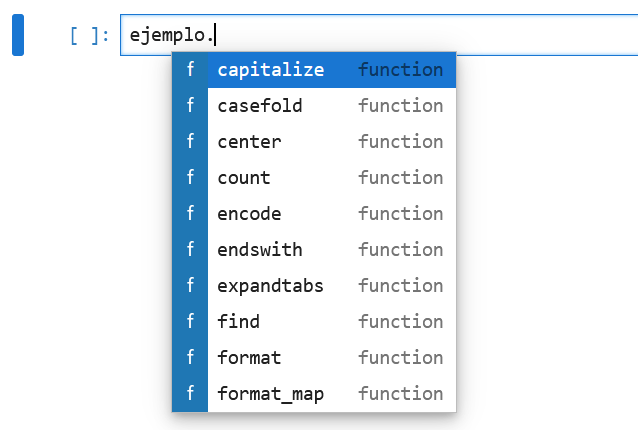
\includegraphics[width=0.5\linewidth,height=\textheight,keepaspectratio]{notebooks/../figuras/metodos_cadenas.png}

\caption{\label{fig-metodos_cadenas}Métodos y atributos de un objeto de
tipo \texttt{str}.}

\end{figure}%

Veamos algunos ejemplos de los métodos de las cadenas.

\begin{Shaded}
\begin{Highlighting}[]
\CommentTok{\# Imprimimos la cadena original}
\BuiltInTok{print}\NormalTok{(ejemplo)}
\end{Highlighting}
\end{Shaded}

\begin{verbatim}
Murciélago
\end{verbatim}

\begin{Shaded}
\begin{Highlighting}[]
\CommentTok{\# Centramos la cadena en 20 espacios}
\BuiltInTok{print}\NormalTok{(ejemplo.center(}\DecValTok{20}\NormalTok{))}
\end{Highlighting}
\end{Shaded}

\begin{verbatim}
     Murciélago     
\end{verbatim}

\begin{Shaded}
\begin{Highlighting}[]
\CommentTok{\# Centramos la cadena en 20 espacios y usamos \textquotesingle{}{-}\textquotesingle{} en los espacios restantes}
\BuiltInTok{print}\NormalTok{(ejemplo.center(}\DecValTok{20}\NormalTok{,}\StringTok{\textquotesingle{}{-}\textquotesingle{}}\NormalTok{)) }
\end{Highlighting}
\end{Shaded}

\begin{verbatim}
-----Murciélago-----
\end{verbatim}

\begin{Shaded}
\begin{Highlighting}[]
\CommentTok{\# Convertimos todos los caracteres a mayúsculas}
\BuiltInTok{print}\NormalTok{(ejemplo.upper())}
\end{Highlighting}
\end{Shaded}

\begin{verbatim}
MURCIÉLAGO
\end{verbatim}

\begin{Shaded}
\begin{Highlighting}[]
\CommentTok{\# Encontrar un caracter dentro de la cadena, }
\CommentTok{\# nos dá el índice (solo de la primera aparición):}
\BuiltInTok{print}\NormalTok{(ejemplo.find(}\StringTok{\textquotesingle{}é\textquotesingle{}}\NormalTok{))}
\end{Highlighting}
\end{Shaded}

\begin{verbatim}
5
\end{verbatim}

\begin{Shaded}
\begin{Highlighting}[]
\CommentTok{\# Cuando el caracter no está en la cadena, regresa un {-}1}
\BuiltInTok{print}\NormalTok{(ejemplo.find(}\StringTok{\textquotesingle{}e\textquotesingle{}}\NormalTok{))}
\end{Highlighting}
\end{Shaded}

\begin{verbatim}
-1
\end{verbatim}

\begin{Shaded}
\begin{Highlighting}[]
\CommentTok{\# Cuenta el número de aparciones de un caracter dentro de la cadena}
\BuiltInTok{print}\NormalTok{(ejemplo.count(}\StringTok{\textquotesingle{}g\textquotesingle{}}\NormalTok{))}
\end{Highlighting}
\end{Shaded}

\begin{verbatim}
1
\end{verbatim}

\begin{Shaded}
\begin{Highlighting}[]
\CommentTok{\# Pregunta si la cadena se puede imprimir}
\BuiltInTok{print}\NormalTok{(ejemplo.isprintable())}
\end{Highlighting}
\end{Shaded}

\begin{verbatim}
True
\end{verbatim}

\begin{Shaded}
\begin{Highlighting}[]
\CommentTok{\# Reemplazamos un caracter o conjunto de caracteres por otro.}
\BuiltInTok{print}\NormalTok{(ejemplo.replace(}\StringTok{\textquotesingle{}é\textquotesingle{}}\NormalTok{, }\StringTok{\textquotesingle{}e\textquotesingle{}}\NormalTok{))}
\end{Highlighting}
\end{Shaded}

\begin{verbatim}
Murcielago
\end{verbatim}

\section{Funciones y operadores sobre
cadenas.}\label{funciones-y-operadores-sobre-cadenas.}

Veamos algunas funciones incorporadas y operadores que se pueden aplicar
sobre las cadenas.

\begin{Shaded}
\begin{Highlighting}[]
\CommentTok{\# Definimos una cadena}
\NormalTok{cadena }\OperatorTok{=} \StringTok{\textquotesingle{}anita lava la tina\textquotesingle{}}
\BuiltInTok{print}\NormalTok{(cadena)}
\end{Highlighting}
\end{Shaded}

\begin{verbatim}
anita lava la tina
\end{verbatim}

\begin{itemize}
\tightlist
\item
  Función \texttt{len()} para obtener la longitud de la cadena.
\end{itemize}

\begin{Shaded}
\begin{Highlighting}[]
\BuiltInTok{print}\NormalTok{(}\BuiltInTok{len}\NormalTok{(cadena))}
\end{Highlighting}
\end{Shaded}

\begin{verbatim}
18
\end{verbatim}

\begin{itemize}
\tightlist
\item
  Funciones \texttt{max()} y \texttt{min()} para obtener el máximo y
  mínimo de acuerdo con su código unicode.
\end{itemize}

\begin{Shaded}
\begin{Highlighting}[]
\BuiltInTok{print}\NormalTok{(}\BuiltInTok{min}\NormalTok{(cadena)) }\CommentTok{\# El mínimo es el espacio en blanco}
\BuiltInTok{print}\NormalTok{(}\BuiltInTok{max}\NormalTok{(cadena))}
\end{Highlighting}
\end{Shaded}

\begin{verbatim}
 
v
\end{verbatim}

\begin{itemize}
\tightlist
\item
  Función \texttt{sorted()} regresa una lista de elementos de la cadena
  ordenados, de acuerdo con su código unicode.
\end{itemize}

\begin{Shaded}
\begin{Highlighting}[]
\BuiltInTok{print}\NormalTok{(}\BuiltInTok{sorted}\NormalTok{(cadena))}
\end{Highlighting}
\end{Shaded}

\begin{verbatim}
[' ', ' ', ' ', 'a', 'a', 'a', 'a', 'a', 'a', 'i', 'i', 'l', 'l', 'n', 'n', 't', 't', 'v']
\end{verbatim}

\begin{itemize}
\tightlist
\item
  Operador \texttt{==} para comparar cadenas
\end{itemize}

\begin{Shaded}
\begin{Highlighting}[]
\NormalTok{cadena\_reversa }\OperatorTok{=}\NormalTok{ cadena[::}\OperatorTok{{-}}\DecValTok{1}\NormalTok{] }\CommentTok{\# construimos la cadena en reversa}
\BuiltInTok{print}\NormalTok{(}\StringTok{\textquotesingle{}original  : \textquotesingle{}}\NormalTok{, cadena)}
\BuiltInTok{print}\NormalTok{(}\StringTok{\textquotesingle{}invertida : \textquotesingle{}}\NormalTok{, cadena\_reversa)}
\BuiltInTok{print}\NormalTok{(}\StringTok{\textquotesingle{}¿Las cadenas son iguales? \textquotesingle{}}\NormalTok{, cadena }\OperatorTok{==}\NormalTok{ cadena\_reversa)}
\end{Highlighting}
\end{Shaded}

\begin{verbatim}
original  :  anita lava la tina
invertida :  anit al aval atina
¿Las cadenas son iguales?  False
\end{verbatim}

Para checar que el contenido de \texttt{cadena} es un palíndromo
tendríamos que eliminar los espacios cuando hacemos la comparación de la
cadena original con la cadena en reversa:

\begin{Shaded}
\begin{Highlighting}[]
\CommentTok{\# Eliminamos los espacios}
\NormalTok{cadena\_original\_sin\_esp }\OperatorTok{=}\NormalTok{ cadena.replace(}\StringTok{\textquotesingle{} \textquotesingle{}}\NormalTok{,}\StringTok{\textquotesingle{}\textquotesingle{}}\NormalTok{)}
\NormalTok{cadena\_reversa\_sin\_esp }\OperatorTok{=}\NormalTok{ cadena\_reversa.replace(}\StringTok{\textquotesingle{} \textquotesingle{}}\NormalTok{,}\StringTok{\textquotesingle{}\textquotesingle{}}\NormalTok{)}

\CommentTok{\# Imprimimos las cadenas}
\BuiltInTok{print}\NormalTok{(}\StringTok{\textquotesingle{}original sin espacios: "\textquotesingle{}}\NormalTok{, cadena\_original\_sin\_esp, }\StringTok{\textquotesingle{}"\textquotesingle{}}\NormalTok{, sep}\OperatorTok{=}\StringTok{\textquotesingle{}\textquotesingle{}}\NormalTok{)}
\BuiltInTok{print}\NormalTok{(}\StringTok{\textquotesingle{}en reversa sin espacios: "\textquotesingle{}}\NormalTok{, cadena\_reversa\_sin\_esp, }\StringTok{\textquotesingle{}"\textquotesingle{}}\NormalTok{, sep}\OperatorTok{=}\StringTok{\textquotesingle{}\textquotesingle{}}\NormalTok{)}

\CommentTok{\# Verificamos si es palíndromo o no}
\BuiltInTok{print}\NormalTok{(}\StringTok{\textquotesingle{}¿Es palíndromo? :\textquotesingle{}}\NormalTok{, cadena\_original\_sin\_esp }\OperatorTok{==}\NormalTok{ cadena\_reversa\_sin\_esp)}
\end{Highlighting}
\end{Shaded}

\begin{verbatim}
original sin espacios: "anitalavalatina"
en reversa sin espacios: "anitalavalatina"
¿Es palíndromo? : True
\end{verbatim}

El siguiente es el mismo algoritmo, pero con un código más reducido
(\emph{pythonico}):

\begin{Shaded}
\begin{Highlighting}[]
\BuiltInTok{print}\NormalTok{(}\StringTok{\textquotesingle{}¿"\textquotesingle{}}\NormalTok{, cadena, }\StringTok{\textquotesingle{}" es palíndromo? \textquotesingle{}}\NormalTok{, cadena.replace(}\StringTok{\textquotesingle{} \textquotesingle{}}\NormalTok{,}\StringTok{\textquotesingle{}\textquotesingle{}}\NormalTok{) }\OperatorTok{==}\NormalTok{ cadena[::}\OperatorTok{{-}}\DecValTok{1}\NormalTok{].replace(}\StringTok{\textquotesingle{} \textquotesingle{}}\NormalTok{,}\StringTok{\textquotesingle{}\textquotesingle{}}\NormalTok{), sep}\OperatorTok{=}\StringTok{\textquotesingle{}\textquotesingle{}}\NormalTok{)}
\end{Highlighting}
\end{Shaded}

\begin{verbatim}
¿"anita lava la tina" es palíndromo? True
\end{verbatim}

\begin{Shaded}
\begin{Highlighting}[]
\CommentTok{\# Usamos el caracter \textbackslash{} para escribir una }
\CommentTok{\# sola instrucción en varias líneas}
\BuiltInTok{print}\NormalTok{(}\StringTok{\textquotesingle{}¿"\textquotesingle{}}\NormalTok{, cadena, }\StringTok{\textquotesingle{}" es palíndromo? \textquotesingle{}}\NormalTok{, }\OperatorTok{\textbackslash{}}
\NormalTok{      cadena.replace(}\StringTok{\textquotesingle{} \textquotesingle{}}\NormalTok{,}\StringTok{\textquotesingle{}\textquotesingle{}}\NormalTok{) }\OperatorTok{==}\NormalTok{ cadena[::}\OperatorTok{{-}}\DecValTok{1}\NormalTok{].replace(}\StringTok{\textquotesingle{} \textquotesingle{}}\NormalTok{,}\StringTok{\textquotesingle{}\textquotesingle{}}\NormalTok{), }\OperatorTok{\textbackslash{}}
\NormalTok{      sep}\OperatorTok{=}\StringTok{\textquotesingle{}\textquotesingle{}}\NormalTok{)}
\end{Highlighting}
\end{Shaded}

\begin{verbatim}
¿"anita lava la tina" es palíndromo? True
\end{verbatim}

\begin{itemize}
\tightlist
\item
  Operador \texttt{in} para saber si un elemento está en la cadena.
\end{itemize}

\begin{Shaded}
\begin{Highlighting}[]
\BuiltInTok{print}\NormalTok{(}\StringTok{\textquotesingle{}v\textquotesingle{}} \KeywordTok{in}\NormalTok{ cadena)}
\end{Highlighting}
\end{Shaded}

\begin{verbatim}
True
\end{verbatim}

\begin{itemize}
\tightlist
\item
  Operador \texttt{+} para concatenar cadenas.
\end{itemize}

\begin{Shaded}
\begin{Highlighting}[]
\NormalTok{palabra }\OperatorTok{=} \StringTok{\textquotesingle{}Palíndromo : \textquotesingle{}}
\BuiltInTok{print}\NormalTok{(palabra }\OperatorTok{+}\NormalTok{ cadena)}
\end{Highlighting}
\end{Shaded}

\begin{verbatim}
Palíndromo : anita lava la tina
\end{verbatim}

\begin{itemize}
\tightlist
\item
  Operador \texttt{*} para repetir la cadena.
\end{itemize}

\begin{Shaded}
\begin{Highlighting}[]
\CommentTok{\# Repetimos la cadena \textquotesingle{}oh yeah \textquotesingle{} 5 veces}
\NormalTok{expresion }\OperatorTok{=} \StringTok{\textquotesingle{}oh yeah \textquotesingle{}} \OperatorTok{*} \DecValTok{5}
\BuiltInTok{print}\NormalTok{(expresion)}
\end{Highlighting}
\end{Shaded}

\begin{verbatim}
oh yeah oh yeah oh yeah oh yeah oh yeah 
\end{verbatim}

\section{Construcción de cadenas}\label{construcciuxf3n-de-cadenas}

Existen varias maneras de construir cadenas, a continuación se revisan
algunos ejemplos.

\subsection{Usando operaciones
básicas.}\label{usando-operaciones-buxe1sicas.}

Los operadores: \texttt{+} y \texttt{*} están definidos para las
cadenas.

Veamos el siguiente ejemplo:

\begin{Shaded}
\begin{Highlighting}[]
\NormalTok{frase1 }\OperatorTok{=} \StringTok{"Somos aquello en lo que creemos"}
\NormalTok{frase2 }\OperatorTok{=} \StringTok{"aún sin darnos cuenta"}

\CommentTok{\# Concatenación de cadenas}
\NormalTok{frase\_total }\OperatorTok{=}\NormalTok{ frase1 }\OperatorTok{+} \StringTok{\textquotesingle{}, \textquotesingle{}} \OperatorTok{+}\NormalTok{ frase2 }\OperatorTok{+} \StringTok{\textquotesingle{}.\textquotesingle{}}

\BuiltInTok{print}\NormalTok{(frase\_total)}
\end{Highlighting}
\end{Shaded}

\begin{verbatim}
Somos aquello en lo que creemos, aún sin darnos cuenta.
\end{verbatim}

En el siguiente ejemplo creamos una cadena de 60 guiones \texttt{-}
usando el operador \texttt{*}:

\begin{Shaded}
\begin{Highlighting}[]
\BuiltInTok{print}\NormalTok{(}\StringTok{\textquotesingle{}{-}\textquotesingle{}} \OperatorTok{*} \DecValTok{60}\NormalTok{)}
\end{Highlighting}
\end{Shaded}

\begin{verbatim}
------------------------------------------------------------
\end{verbatim}

Escribimos la \texttt{frase\_total} centrada en 60 espacios y entre dos
líneas:

\begin{Shaded}
\begin{Highlighting}[]
\BuiltInTok{print}\NormalTok{(}\StringTok{\textquotesingle{}{-}\textquotesingle{}} \OperatorTok{*} \DecValTok{60}\NormalTok{)}
\BuiltInTok{print}\NormalTok{(frase\_total.center(}\DecValTok{60}\NormalTok{))}
\BuiltInTok{print}\NormalTok{(}\StringTok{\textquotesingle{}{-}\textquotesingle{}} \OperatorTok{*} \DecValTok{60}\NormalTok{)}
\end{Highlighting}
\end{Shaded}

\begin{verbatim}
------------------------------------------------------------
  Somos aquello en lo que creemos, aún sin darnos cuenta.   
------------------------------------------------------------
\end{verbatim}

Podemos agregar al autor de la frase:

\begin{Shaded}
\begin{Highlighting}[]
\BuiltInTok{print}\NormalTok{(}\StringTok{\textquotesingle{}{-}\textquotesingle{}} \OperatorTok{*} \DecValTok{60}\NormalTok{)}
\BuiltInTok{print}\NormalTok{(frase\_total.center(}\DecValTok{60}\NormalTok{))}
\BuiltInTok{print}\NormalTok{(}\StringTok{"Carlos Monsivais"}\NormalTok{.rjust(}\DecValTok{60}\NormalTok{))}
\BuiltInTok{print}\NormalTok{(}\StringTok{\textquotesingle{}{-}\textquotesingle{}} \OperatorTok{*} \DecValTok{60}\NormalTok{)}
\end{Highlighting}
\end{Shaded}

\begin{verbatim}
------------------------------------------------------------
  Somos aquello en lo que creemos, aún sin darnos cuenta.   
                                            Carlos Monsivais
------------------------------------------------------------
\end{verbatim}

Observa que aplicamos el método \texttt{rjust()} para justificar a la
derecha, y lo hicimos directamente en el momento de la creación de la
cadena \texttt{"Carlos\ Monsivais"} (al vuelo).

\subsection{Concatenación y casting}\label{concatenaciuxf3n-y-casting}

Vamos a crear la siguiente cadena:
\texttt{Pedro\ Páramo\ tiene\ 15\ años\ y\ pesa\ 70.5\ kg}.

Usaremos el operador \texttt{+} y contruiremos la cadena usando algunas
variables; convertiremos algunas variables a tipo \texttt{str}:

\begin{Shaded}
\begin{Highlighting}[]
\CommentTok{\# Definimos las siguientes variables}
\NormalTok{edad }\OperatorTok{=} \DecValTok{15}
\NormalTok{nombre }\OperatorTok{=} \StringTok{\textquotesingle{}Pedro\textquotesingle{}}
\NormalTok{apellido }\OperatorTok{=} \StringTok{\textquotesingle{}Páramo\textquotesingle{}}
\NormalTok{peso }\OperatorTok{=} \FloatTok{70.5}

\CommentTok{\# Construimos la cadena usando el operador \textquotesingle{}+\textquotesingle{} y la función \textquotesingle{}str()\textquotesingle{} }
\NormalTok{datos }\OperatorTok{=}\NormalTok{ nombre }\OperatorTok{+}\NormalTok{ apellido }\OperatorTok{+} \StringTok{\textquotesingle{}tiene\textquotesingle{}} \OperatorTok{+} \BuiltInTok{str}\NormalTok{(}\DecValTok{15}\NormalTok{) }\OperatorTok{+} \StringTok{\textquotesingle{}años y pesa\textquotesingle{}} \OperatorTok{+} \BuiltInTok{str}\NormalTok{(}\FloatTok{70.5}\NormalTok{) }\OperatorTok{+} \StringTok{\textquotesingle{}kg\textquotesingle{}}

\BuiltInTok{print}\NormalTok{(datos)}
\end{Highlighting}
\end{Shaded}

\begin{verbatim}
PedroPáramotiene15años y pesa70.5kg
\end{verbatim}

Para agregar espacios es necesario hacerlo de manera explícita como
sigue:

\begin{Shaded}
\begin{Highlighting}[]
\NormalTok{datos }\OperatorTok{=}\NormalTok{ nombre }\OperatorTok{+} \StringTok{\textquotesingle{} \textquotesingle{}} \OperatorTok{+}\NormalTok{ apellido }\OperatorTok{+} \StringTok{\textquotesingle{} tiene \textquotesingle{}} \OperatorTok{+} \BuiltInTok{str}\NormalTok{(}\DecValTok{15}\NormalTok{) }\OperatorTok{+} \StringTok{\textquotesingle{} años y pesa \textquotesingle{}} \OperatorTok{+} \BuiltInTok{str}\NormalTok{(}\FloatTok{70.5}\NormalTok{) }\OperatorTok{+} \StringTok{\textquotesingle{} kg\textquotesingle{}}
\BuiltInTok{print}\NormalTok{(datos)}
\end{Highlighting}
\end{Shaded}

\begin{verbatim}
Pedro Páramo tiene 15 años y pesa 70.5 kg
\end{verbatim}

\subsection{\texorpdfstring{Método
\texttt{str.format()}}{Método str.format()}}\label{muxe9todo-str.format}

Este método permite sustituir variables en los lugares indicados por
\texttt{\{\}}:

\begin{Shaded}
\begin{Highlighting}[]
\NormalTok{datos }\OperatorTok{=} \StringTok{\textquotesingle{}}\SpecialCharTok{\{\}}\StringTok{ }\SpecialCharTok{\{\}}\StringTok{ tiene }\SpecialCharTok{\{\}}\StringTok{ años y pesa }\SpecialCharTok{\{\}}\StringTok{ kg\textquotesingle{}}\NormalTok{.}\BuiltInTok{format}\NormalTok{(nombre, apellido, edad, peso)}
\BuiltInTok{print}\NormalTok{(datos)}
\end{Highlighting}
\end{Shaded}

\begin{verbatim}
Pedro Páramo tiene 15 años y pesa 70.5 kg
\end{verbatim}

Observa que aplicamos el método \texttt{format()} a la cadena en
construcción.

\subsection{\texorpdfstring{Cadenas formateadas (\emph{f-string},
\emph{formatted string
literals})}{Cadenas formateadas (f-string, formatted string literals)}}\label{cadenas-formateadas-f-string-formatted-string-literals}

Este tipo de cadenas permite sustituir variables en los lugares
indicados:

\begin{Shaded}
\begin{Highlighting}[]
\NormalTok{datos }\OperatorTok{=} \SpecialStringTok{f\textquotesingle{}}\SpecialCharTok{\{}\NormalTok{nombre}\SpecialCharTok{\}}\SpecialStringTok{ }\SpecialCharTok{\{}\NormalTok{apellido}\SpecialCharTok{\}}\SpecialStringTok{ tiene }\SpecialCharTok{\{}\NormalTok{edad}\SpecialCharTok{\}}\SpecialStringTok{ años y pesa }\SpecialCharTok{\{}\NormalTok{peso}\SpecialCharTok{\}}\SpecialStringTok{ kg\textquotesingle{}}
\BuiltInTok{print}\NormalTok{(datos)}
\end{Highlighting}
\end{Shaded}

\begin{verbatim}
Pedro Páramo tiene 15 años y pesa 70.5 kg
\end{verbatim}

Observa que agregamos una \texttt{f} al principio de la definición de la
cadena para indicar que se trata de una cadena formateada.

\subsection{\texorpdfstring{Cadenas usando el método
\texttt{str.join()}}{Cadenas usando el método str.join()}}\label{cadenas-usando-el-muxe9todo-str.join}

Dada una cadena que funciona como separador, este método recibe una
estructura de datos que contiene las cadenas que se van a unir y que
estarán separados por la cadena inicial:

\begin{Shaded}
\begin{Highlighting}[]
\NormalTok{datos }\OperatorTok{=} \StringTok{" "}\NormalTok{.join([nombre, apellido, }\StringTok{\textquotesingle{}tiene\textquotesingle{}}\NormalTok{, }\BuiltInTok{str}\NormalTok{(}\DecValTok{15}\NormalTok{), }\StringTok{\textquotesingle{}años y pesa\textquotesingle{}}\NormalTok{, }\BuiltInTok{str}\NormalTok{(}\FloatTok{70.5}\NormalTok{), }\StringTok{\textquotesingle{}kg\textquotesingle{}}\NormalTok{])}
\BuiltInTok{print}\NormalTok{(datos)}
\end{Highlighting}
\end{Shaded}

\begin{verbatim}
Pedro Páramo tiene 15 años y pesa 70.5 kg
\end{verbatim}

En el ejemplo anterior la cadena inicial es un espacio \texttt{"\ "} y
junta todos los elementos que se dan entre corchetes \texttt{{[}{]}}. El
uso de corchetes construye una lista, que es un tipo de dato que se
describe en la Capítulo~\ref{sec-listas}.

\section{Formato de la salida.}\label{formato-de-la-salida.}

Es posible utilizar algunos modificadores en la definición de una cadena
para que se imprima con un cierto formato. Esto aplica para cadenas
formateadas y para el método \texttt{format}. Veamos algunos ejemplos.

\subsection{Texto.}\label{texto.}

\begin{Shaded}
\begin{Highlighting}[]
\CommentTok{\# Impresión del nombre en 30 espacios de texto}
\NormalTok{sdef }\OperatorTok{=} \SpecialStringTok{f\textquotesingle{}}\SpecialCharTok{\{}\NormalTok{nombre}\SpecialCharTok{:30s\}}\SpecialStringTok{\textquotesingle{}}  \CommentTok{\# Alineación a la izq. por omisión}
\NormalTok{sder }\OperatorTok{=} \SpecialStringTok{f\textquotesingle{}}\SpecialCharTok{\{}\NormalTok{nombre}\SpecialCharTok{:\textgreater{}30s\}}\SpecialStringTok{\textquotesingle{}} \CommentTok{\# Alineación a la der.}
\NormalTok{sizq }\OperatorTok{=} \SpecialStringTok{f\textquotesingle{}}\SpecialCharTok{\{}\NormalTok{nombre}\SpecialCharTok{:\textless{}30s\}}\SpecialStringTok{\textquotesingle{}} \CommentTok{\# Alineación a la izq.}
\NormalTok{scen }\OperatorTok{=} \SpecialStringTok{f\textquotesingle{}}\SpecialCharTok{\{}\NormalTok{nombre}\SpecialCharTok{:\^{}30s\}}\SpecialStringTok{\textquotesingle{}} \CommentTok{\# Centrada}
\end{Highlighting}
\end{Shaded}

\begin{Shaded}
\begin{Highlighting}[]
\BuiltInTok{print}\NormalTok{(sdef)}
\BuiltInTok{print}\NormalTok{(sder)}
\BuiltInTok{print}\NormalTok{(sizq)}
\BuiltInTok{print}\NormalTok{(scen)}
\end{Highlighting}
\end{Shaded}

\begin{verbatim}
Pedro                         
                         Pedro
Pedro                         
            Pedro             
\end{verbatim}

Ahora agregamos las cadenas \texttt{-\/-\/-\textbar{}} y
\texttt{\textbar{}-\/-\/-} para delimitar los 30 espacios.

\begin{Shaded}
\begin{Highlighting}[]
\CommentTok{\# Impresión del nombre en 30 espacios de texto}
\NormalTok{sdef }\OperatorTok{=} \SpecialStringTok{f\textquotesingle{}{-}{-}{-}|}\SpecialCharTok{\{}\NormalTok{nombre}\SpecialCharTok{:30s\}}\SpecialStringTok{|{-}{-}{-}\textquotesingle{}}  \CommentTok{\# Alineación a la izq. por omisión}
\NormalTok{sder }\OperatorTok{=} \SpecialStringTok{f\textquotesingle{}{-}{-}{-}|}\SpecialCharTok{\{}\NormalTok{nombre}\SpecialCharTok{:\textgreater{}30s\}}\SpecialStringTok{|{-}{-}{-}\textquotesingle{}} \CommentTok{\# Alineación a la der.}
\NormalTok{sizq }\OperatorTok{=} \SpecialStringTok{f\textquotesingle{}{-}{-}{-}|}\SpecialCharTok{\{}\NormalTok{nombre}\SpecialCharTok{:\textless{}30s\}}\SpecialStringTok{|{-}{-}{-}\textquotesingle{}} \CommentTok{\# Alineación a la izq.}
\NormalTok{scen }\OperatorTok{=} \SpecialStringTok{f\textquotesingle{}{-}{-}{-}|}\SpecialCharTok{\{}\NormalTok{nombre}\SpecialCharTok{:\^{}30s\}}\SpecialStringTok{|{-}{-}{-}\textquotesingle{}} \CommentTok{\# Centrada}

\BuiltInTok{print}\NormalTok{(sdef)}
\BuiltInTok{print}\NormalTok{(sder)}
\BuiltInTok{print}\NormalTok{(sizq)}
\BuiltInTok{print}\NormalTok{(scen)}
\end{Highlighting}
\end{Shaded}

\begin{verbatim}
---|Pedro                         |---
---|                         Pedro|---
---|Pedro                         |---
---|            Pedro             |---
\end{verbatim}

\begin{tcolorbox}[enhanced jigsaw, breakable, colback=white, bottomrule=.15mm, colframe=quarto-callout-note-color-frame, coltitle=black, colbacktitle=quarto-callout-note-color!10!white, toprule=.15mm, leftrule=.75mm, arc=.35mm, toptitle=1mm, bottomtitle=1mm, titlerule=0mm, rightrule=.15mm, title=\textcolor{quarto-callout-note-color}{\faInfo}\hspace{0.5em}{Nota.}, opacityback=0, opacitybacktitle=0.6, left=2mm]

Observa que en el ejemplo anterior se usó una \texttt{s} al final del
número \texttt{30}, esto es para indicar que la variable \texttt{nombre}
es de tipo cadena. Para enteros en base diez se usa una \texttt{d} y
para flotantes una \texttt{f}. Estas terminaciones no son necesarias
aunque es conveniente agregarlas para hacer el código más claro y que no
haya errores de formato.

Más información la puedes consultar en: Format Specification
Mini-Language

\end{tcolorbox}

\subsection{Enteros}\label{enteros}

Para números enteros podemos definir el número de espacios y alinear la
salida:

\begin{Shaded}
\begin{Highlighting}[]
\CommentTok{\# Este es un formato de número entero que usa \_ para separar los miles}
\NormalTok{n1 }\OperatorTok{=} \DecValTok{5\_521\_345\_678}
\NormalTok{n2 }\OperatorTok{=} \DecValTok{7\_712\_932\_143}
\NormalTok{n3 }\OperatorTok{=} \DecValTok{8\_123\_535\_098}

\NormalTok{idef }\OperatorTok{=} \SpecialStringTok{f\textquotesingle{}{-}{-}{-}|}\SpecialCharTok{\{}\NormalTok{n1}\SpecialCharTok{:15d\}}\SpecialStringTok{|{-}{-}{-}\textquotesingle{}}  \CommentTok{\# alineación a la der. por omisión}
\NormalTok{icen }\OperatorTok{=} \SpecialStringTok{f\textquotesingle{}{-}{-}{-}|}\SpecialCharTok{\{}\NormalTok{n1}\SpecialCharTok{:\^{}15d\}}\SpecialStringTok{|{-}{-}{-}\textquotesingle{}} \CommentTok{\# centrado}
\NormalTok{iizq }\OperatorTok{=} \SpecialStringTok{f\textquotesingle{}{-}{-}{-}|}\SpecialCharTok{\{}\NormalTok{n2}\SpecialCharTok{:\textless{}15d\}}\SpecialStringTok{|{-}{-}{-}\textquotesingle{}} \CommentTok{\# alineación a la izq.}
\NormalTok{ider }\OperatorTok{=} \SpecialStringTok{f\textquotesingle{}{-}{-}{-}|}\SpecialCharTok{\{}\NormalTok{n3}\SpecialCharTok{:\textgreater{}15d\}}\SpecialStringTok{|{-}{-}{-}\textquotesingle{}} \CommentTok{\# alineación a la der.}

\BuiltInTok{print}\NormalTok{(idef, icen, iizq, ider, sep}\OperatorTok{=}\StringTok{\textquotesingle{}}\CharTok{\textbackslash{}n}\StringTok{\textquotesingle{}}\NormalTok{)}
\end{Highlighting}
\end{Shaded}

\begin{verbatim}
---|     5521345678|---
---|  5521345678   |---
---|7712932143     |---
---|     8123535098|---
\end{verbatim}

También es posible usar \texttt{,} como separador de los miles en la
salida, veamos:

\begin{Shaded}
\begin{Highlighting}[]
\NormalTok{idef }\OperatorTok{=} \SpecialStringTok{f\textquotesingle{}{-}{-}{-}|}\SpecialCharTok{\{}\NormalTok{n1}\SpecialCharTok{:15,d\}}\SpecialStringTok{|{-}{-}{-}\textquotesingle{}}  \CommentTok{\# alineación a la der. por omisión}
\NormalTok{icen }\OperatorTok{=} \SpecialStringTok{f\textquotesingle{}{-}{-}{-}|}\SpecialCharTok{\{}\NormalTok{n1}\SpecialCharTok{:\^{}15,d\}}\SpecialStringTok{|{-}{-}{-}\textquotesingle{}} \CommentTok{\# centrado}
\NormalTok{iizq }\OperatorTok{=} \SpecialStringTok{f\textquotesingle{}{-}{-}{-}|}\SpecialCharTok{\{}\NormalTok{n2}\SpecialCharTok{:\textless{}15,d\}}\SpecialStringTok{|{-}{-}{-}\textquotesingle{}} \CommentTok{\# alineación a la izq.}
\NormalTok{ider }\OperatorTok{=} \SpecialStringTok{f\textquotesingle{}{-}{-}{-}|}\SpecialCharTok{\{}\NormalTok{n3}\SpecialCharTok{:\textgreater{}15,d\}}\SpecialStringTok{|{-}{-}{-}\textquotesingle{}} \CommentTok{\# alineación a la der.}

\BuiltInTok{print}\NormalTok{(idef, icen, iizq, ider, sep}\OperatorTok{=}\StringTok{\textquotesingle{}}\CharTok{\textbackslash{}n}\StringTok{\textquotesingle{}}\NormalTok{)}
\end{Highlighting}
\end{Shaded}

\begin{verbatim}
---|  5,521,345,678|---
---| 5,521,345,678 |---
---|7,712,932,143  |---
---|  8,123,535,098|---
\end{verbatim}

Y se puede completar con \texttt{0}'s los espacios en blanco:

\begin{Shaded}
\begin{Highlighting}[]
\NormalTok{idef }\OperatorTok{=} \SpecialStringTok{f\textquotesingle{}{-}{-}{-}|}\SpecialCharTok{\{}\NormalTok{n1}\SpecialCharTok{:015,d\}}\SpecialStringTok{|{-}{-}{-}\textquotesingle{}}  \CommentTok{\# alineación a la der. por omisión}
\NormalTok{icen }\OperatorTok{=} \SpecialStringTok{f\textquotesingle{}{-}{-}{-}|}\SpecialCharTok{\{}\NormalTok{n1}\SpecialCharTok{:\^{}015,d\}}\SpecialStringTok{|{-}{-}{-}\textquotesingle{}} \CommentTok{\# centrado}
\NormalTok{iizq }\OperatorTok{=} \SpecialStringTok{f\textquotesingle{}{-}{-}{-}|}\SpecialCharTok{\{}\NormalTok{n2}\SpecialCharTok{:\textless{}015,d\}}\SpecialStringTok{|{-}{-}{-}\textquotesingle{}} \CommentTok{\# alineación a la izq.}
\NormalTok{ider }\OperatorTok{=} \SpecialStringTok{f\textquotesingle{}{-}{-}{-}|}\SpecialCharTok{\{}\NormalTok{n3}\SpecialCharTok{:\textgreater{}015,d\}}\SpecialStringTok{|{-}{-}{-}\textquotesingle{}} \CommentTok{\# alineación a la der.}

\BuiltInTok{print}\NormalTok{(idef, icen, iizq, ider, sep}\OperatorTok{=}\StringTok{\textquotesingle{}}\CharTok{\textbackslash{}n}\StringTok{\textquotesingle{}}\NormalTok{)}
\end{Highlighting}
\end{Shaded}

\begin{verbatim}
---|005,521,345,678|---
---|05,521,345,6780|---
---|7,712,932,14300|---
---|008,123,535,098|---
\end{verbatim}

Se puede generar la salida de un entero en las bases decimal,
hexadecimal, octal o binaria usando \texttt{d}, \texttt{x}, \texttt{o} y
\texttt{b} respectivamente.

\begin{Shaded}
\begin{Highlighting}[]
\NormalTok{ejemplo }\OperatorTok{=} \DecValTok{16}
\BuiltInTok{print}\NormalTok{(}\SpecialStringTok{f\textquotesingle{}int: }\SpecialCharTok{\{}\NormalTok{ejemplo}\SpecialCharTok{:d\}}\SpecialStringTok{\textquotesingle{}}\NormalTok{)}
\BuiltInTok{print}\NormalTok{(}\SpecialStringTok{f\textquotesingle{}hex: }\SpecialCharTok{\{}\NormalTok{ejemplo}\SpecialCharTok{:x\}}\SpecialStringTok{\textquotesingle{}}\NormalTok{)}
\BuiltInTok{print}\NormalTok{(}\SpecialStringTok{f\textquotesingle{}oct: }\SpecialCharTok{\{}\NormalTok{ejemplo}\SpecialCharTok{:o\}}\SpecialStringTok{\textquotesingle{}}\NormalTok{)}
\BuiltInTok{print}\NormalTok{(}\SpecialStringTok{f\textquotesingle{}bin: }\SpecialCharTok{\{}\NormalTok{ejemplo}\SpecialCharTok{:b\}}\SpecialStringTok{\textquotesingle{}}\NormalTok{)}
\end{Highlighting}
\end{Shaded}

\begin{verbatim}
int: 16
hex: 10
oct: 20
bin: 10000
\end{verbatim}

\subsection{Flotantes}\label{flotantes}

En el caso de números flotantes se puede definir el número de decimales
en la salida:

\begin{Shaded}
\begin{Highlighting}[]
\CommentTok{\# Valor aproximado de pi}
\NormalTok{pi }\OperatorTok{=} \DecValTok{3} \OperatorTok{+} \DecValTok{1}\OperatorTok{/}\DecValTok{7}

\CommentTok{\# Cadena con 5 decimales de pi:}
\NormalTok{spi }\OperatorTok{=} \SpecialStringTok{f\textquotesingle{}}\SpecialCharTok{\{}\NormalTok{pi}\SpecialCharTok{:.5f\}}\SpecialStringTok{\textquotesingle{}}

\BuiltInTok{print}\NormalTok{(}\StringTok{\textquotesingle{}El valor de PI es aproximadamente\textquotesingle{}}\NormalTok{, spi) }
\end{Highlighting}
\end{Shaded}

\begin{verbatim}
El valor de PI es aproximadamente 3.14286
\end{verbatim}

Y también es posible definir el número total de espacios que incluyen la
parte entera, el punto decimal y el número de decimales:

\begin{Shaded}
\begin{Highlighting}[]
\NormalTok{numero\_flotante\_grande }\OperatorTok{=} \FloatTok{213.2131255345435643}

\CommentTok{\# Cadena con 15 espacios totales y 3 decimales}
\NormalTok{snumero }\OperatorTok{=} \SpecialStringTok{f\textquotesingle{}}\SpecialCharTok{\{}\NormalTok{numero\_flotante\_grande}\SpecialCharTok{:15.3f\}}\SpecialStringTok{\textquotesingle{}}

\BuiltInTok{print}\NormalTok{(}\SpecialStringTok{f\textquotesingle{}{-}{-}{-}|}\SpecialCharTok{\{}\NormalTok{snumero}\SpecialCharTok{\}}\SpecialStringTok{|{-}{-}{-}\textquotesingle{}}\NormalTok{)}
\end{Highlighting}
\end{Shaded}

\begin{verbatim}
---|        213.213|---
\end{verbatim}

Al igual que las cadenas y los enteros, también se puede usar una
alineación en la salida y rellenar con ceros los espacios en blanco:

\begin{Shaded}
\begin{Highlighting}[]
\NormalTok{snum\_cen }\OperatorTok{=} \SpecialStringTok{f\textquotesingle{}}\SpecialCharTok{\{}\NormalTok{numero\_flotante\_grande}\SpecialCharTok{:\^{}015.3f\}}\SpecialStringTok{\textquotesingle{}}
\NormalTok{snum\_izq }\OperatorTok{=} \SpecialStringTok{f\textquotesingle{}}\SpecialCharTok{\{}\NormalTok{numero\_flotante\_grande}\SpecialCharTok{:\textless{}015.3f\}}\SpecialStringTok{\textquotesingle{}}
\NormalTok{snum\_der }\OperatorTok{=} \SpecialStringTok{f\textquotesingle{}}\SpecialCharTok{\{}\NormalTok{numero\_flotante\_grande}\SpecialCharTok{:\textgreater{}015.3f\}}\SpecialStringTok{\textquotesingle{}}

\BuiltInTok{print}\NormalTok{(snum\_cen)}
\BuiltInTok{print}\NormalTok{(snum\_izq)}
\BuiltInTok{print}\NormalTok{(snum\_der)}
\end{Highlighting}
\end{Shaded}

\begin{verbatim}
0000213.2130000
213.21300000000
00000000213.213
\end{verbatim}

\subsection{\texorpdfstring{Usando el método
\texttt{format()}}{Usando el método format()}}\label{usando-el-muxe9todo-format}

Usando el método \texttt{str.format()}, también podemos formatear la
salida. Aplica exactamente lo mismo que con las \emph{f-string}. Por
ejemplo:

\begin{Shaded}
\begin{Highlighting}[]
\CommentTok{\# Definimos dos números enteros}
\NormalTok{votos\_a\_favor }\OperatorTok{=} \DecValTok{42\_572\_654}   
\NormalTok{votos\_en\_contra }\OperatorTok{=} \DecValTok{43\_132\_495} 

\CommentTok{\# Realizamos algunas operaciones}
\NormalTok{total\_de\_votos }\OperatorTok{=}\NormalTok{ votos\_a\_favor }\OperatorTok{+}\NormalTok{ votos\_en\_contra}
\NormalTok{porcentaje }\OperatorTok{=}\NormalTok{ votos\_a\_favor }\OperatorTok{/}\NormalTok{ total\_de\_votos}

\CommentTok{\# Revisamos el contenido y tipo de los números}
\BuiltInTok{print}\NormalTok{(votos\_a\_favor, }\BuiltInTok{type}\NormalTok{(votos\_a\_favor))}
\BuiltInTok{print}\NormalTok{(votos\_en\_contra, }\BuiltInTok{type}\NormalTok{(votos\_en\_contra))}
\BuiltInTok{print}\NormalTok{(total\_de\_votos, }\BuiltInTok{type}\NormalTok{(total\_de\_votos))}
\BuiltInTok{print}\NormalTok{(porcentaje, }\BuiltInTok{type}\NormalTok{(porcentaje))}

\CommentTok{\# Realizamos la impresión usando un formato}
\BuiltInTok{print}\NormalTok{(}\StringTok{\textquotesingle{}}\SpecialCharTok{\{:\^{}20d\}}\StringTok{ votos a favor (}\SpecialCharTok{\{:\^{}10.2\%\}}\StringTok{)\textquotesingle{}}\NormalTok{.}\BuiltInTok{format}\NormalTok{(votos\_a\_favor, porcentaje))}
\end{Highlighting}
\end{Shaded}

\begin{verbatim}
42572654 <class 'int'>
43132495 <class 'int'>
85705149 <class 'int'>
0.496733912684756 <class 'float'>
      42572654       votos a favor (  49.67%  )
\end{verbatim}

Observa que se imprime \texttt{votos\_a\_favor} en 20 espacios y
alineado al centro. También se imprime \texttt{porcentaje}, que es un
número flotante, usando 10 espacios que incluyen el punto, dos decimales
y el símbolo \texttt{\%}. El uso de \texttt{\%} convierte el número
flotante en un porcentaje (multiplica por 100) automáticamente e imprime
el símbolo.

Se pueden usar números para identificar los argumentos de
\texttt{str.format()}:

\begin{Shaded}
\begin{Highlighting}[]
\NormalTok{ej1 }\OperatorTok{=} \StringTok{\textquotesingle{}}\SpecialCharTok{\{0\}}\StringTok{ y }\SpecialCharTok{\{1\}}\StringTok{\textquotesingle{}}\NormalTok{.}\BuiltInTok{format}\NormalTok{(}\StringTok{\textquotesingle{}el huevo\textquotesingle{}}\NormalTok{, }\StringTok{\textquotesingle{}la gallina\textquotesingle{}}\NormalTok{)}
\NormalTok{ej2 }\OperatorTok{=} \StringTok{\textquotesingle{}}\SpecialCharTok{\{1\}}\StringTok{ y }\SpecialCharTok{\{0:\^{}20s\}}\StringTok{\textquotesingle{}}\NormalTok{.}\BuiltInTok{format}\NormalTok{(}\StringTok{\textquotesingle{}el huevo\textquotesingle{}}\NormalTok{, }\StringTok{\textquotesingle{}la gallina\textquotesingle{}}\NormalTok{)}

\BuiltInTok{print}\NormalTok{(ej1)}
\BuiltInTok{print}\NormalTok{(ej2)}
\end{Highlighting}
\end{Shaded}

\begin{verbatim}
el huevo y la gallina
la gallina y       el huevo      
\end{verbatim}

Se le puede dar nombre a los argumentos para que sea más fácil entender
la salida

\begin{Shaded}
\begin{Highlighting}[]
\NormalTok{ej3 }\OperatorTok{=} \StringTok{"Look }\SpecialCharTok{\{sujeto\}}\StringTok{, there\textquotesingle{}s an }\SpecialCharTok{\{objeto\}}\StringTok{ up in the sky"}\NormalTok{.}\BuiltInTok{format}\NormalTok{(sujeto}\OperatorTok{=}\StringTok{\textquotesingle{}mummy\textquotesingle{}}\NormalTok{, objeto}\OperatorTok{=}\StringTok{\textquotesingle{}aeroplane\textquotesingle{}}\NormalTok{)}

\BuiltInTok{print}\NormalTok{(ej3)}
\end{Highlighting}
\end{Shaded}

\begin{verbatim}
Look mummy, there's an aeroplane up in the sky
\end{verbatim}

Usar un nombre en los argumentos de \texttt{str.format()} permite
ponerlos en cualquier orden:

\begin{Shaded}
\begin{Highlighting}[]
\NormalTok{ej4 }\OperatorTok{=} \StringTok{"Look }\SpecialCharTok{\{sujeto\}}\StringTok{, there\textquotesingle{}s an }\SpecialCharTok{\{objeto\}}\StringTok{ up in the sky"}\NormalTok{.}\BuiltInTok{format}\NormalTok{(objeto}\OperatorTok{=}\StringTok{\textquotesingle{}aeroplane\textquotesingle{}}\NormalTok{, sujeto}\OperatorTok{=}\StringTok{\textquotesingle{}mummy\textquotesingle{}}\NormalTok{)}

\BuiltInTok{print}\NormalTok{(ej4)}
\end{Highlighting}
\end{Shaded}

\begin{verbatim}
Look mummy, there's an aeroplane up in the sky
\end{verbatim}

Se pueden combinar números con nombres de argumento:

\begin{Shaded}
\begin{Highlighting}[]
\NormalTok{ej5 }\OperatorTok{=} \StringTok{\textquotesingle{}El }\SpecialCharTok{\{0\}}\StringTok{, el }\SpecialCharTok{\{1\}}\StringTok{, y el }\SpecialCharTok{\{otro\}}\StringTok{.\textquotesingle{}}\NormalTok{.}\BuiltInTok{format}\NormalTok{(}\StringTok{\textquotesingle{}Bueno\textquotesingle{}}\NormalTok{, }\StringTok{\textquotesingle{}Malo\textquotesingle{}}\NormalTok{, otro}\OperatorTok{=}\StringTok{\textquotesingle{}Feo\textquotesingle{}}\NormalTok{)}

\BuiltInTok{print}\NormalTok{(ej5)}
\end{Highlighting}
\end{Shaded}

\begin{verbatim}
El Bueno, el Malo, y el Feo.
\end{verbatim}

Otro ejemplo de alineación (la declaración \texttt{for} la revisaremos
en la Capítulo~\ref{sec-control_de_flujo}:

\begin{Shaded}
\begin{Highlighting}[]
\ControlFlowTok{for}\NormalTok{ x }\KeywordTok{in} \BuiltInTok{range}\NormalTok{(}\DecValTok{1}\NormalTok{, }\DecValTok{11}\NormalTok{):}
    \BuiltInTok{print}\NormalTok{(}\StringTok{\textquotesingle{}}\SpecialCharTok{\{0:2d\}}\StringTok{ }\SpecialCharTok{\{1:3d\}}\StringTok{ }\SpecialCharTok{\{2:4d\}}\StringTok{\textquotesingle{}}\NormalTok{.}\BuiltInTok{format}\NormalTok{(x, x}\OperatorTok{*}\NormalTok{x, x}\OperatorTok{*}\NormalTok{x}\OperatorTok{*}\NormalTok{x))}
\end{Highlighting}
\end{Shaded}

\begin{verbatim}
 1   1    1
 2   4    8
 3   9   27
 4  16   64
 5  25  125
 6  36  216
 7  49  343
 8  64  512
 9  81  729
10 100 1000
\end{verbatim}

Para más información véase Format String Syntax

\subsection{Método antiguo para formateo de la
salida.}\label{muxe9todo-antiguo-para-formateo-de-la-salida.}

Se puede seguir usando la forma antigua para formatearla salida, la cual
es heredada del lengueaje C.

\begin{Shaded}
\begin{Highlighting}[]
\NormalTok{viejo }\OperatorTok{=} \StringTok{\textquotesingle{}El valor aproximado de pi es }\SpecialCharTok{\%10.6f}\StringTok{.\textquotesingle{}} \OperatorTok{\%}\NormalTok{ pi}

\BuiltInTok{print}\NormalTok{(viejo)}
\end{Highlighting}
\end{Shaded}

\begin{verbatim}
El valor aproximado de pi es   3.142857.
\end{verbatim}

\section{Inmutabilidad de las
cadenas}\label{inmutabilidad-de-las-cadenas}

Los elementos de las cadenas no se pueden modificar:

\begin{Shaded}
\begin{Highlighting}[]
\CommentTok{\# Intentamos modificar el elemento 5 de la cadena}
\NormalTok{ejemplo[}\DecValTok{5}\NormalTok{] }\OperatorTok{=} \StringTok{"e"}
\end{Highlighting}
\end{Shaded}

\begin{Highlighting}
\textcolor{black}{TypeError: 'int' object does not support item assignment}
\textcolor{black}{}\textcolor{QuartoInternalColor1}{---------------------------------------------------------------------------}\textcolor{QuartoInternalColor2}{}
\textcolor{QuartoInternalColor2}{}\textcolor{QuartoInternalColor1}{TypeError}\textcolor{QuartoInternalColor2}{                                 Traceback (most recent call last)}
\textcolor{QuartoInternalColor2}{}\textcolor{QuartoInternalColor3}{Cell}\textcolor{QuartoInternalColor2}{}\textcolor{QuartoInternalColor3}{ }\textcolor{QuartoInternalColor2}{}\textcolor{QuartoInternalColor4}{In[112]}\textcolor{QuartoInternalColor2}{}\textcolor{QuartoInternalColor4}{, line 2}\textcolor{QuartoInternalColor2}{}
\textcolor{QuartoInternalColor2}{}\textcolor{QuartoInternalColor4}{      1}\textcolor{QuartoInternalColor2}{ }\textcolor{QuartoInternalColor6}{# Intentamos modificar el elemento 5 de la cadena}\textcolor{QuartoInternalColor2}{}
\textcolor{QuartoInternalColor2}{}\textcolor{QuartoInternalColor4}{----> }\textcolor{QuartoInternalColor2}{}\textcolor{QuartoInternalColor4}{2}\textcolor{QuartoInternalColor2}{ }\textcolor{QuartoInternalColor2}{ejemplo}\textcolor{QuartoInternalColor2}{}\textcolor{QuartoInternalColor2}{[}\textcolor{QuartoInternalColor2}{}\textcolor{QuartoInternalColor2}{5}\textcolor{QuartoInternalColor2}{}\textcolor{QuartoInternalColor2}{]}\textcolor{QuartoInternalColor2}{ = }\textcolor{QuartoInternalColor7}{"}\textcolor{QuartoInternalColor2}{}\textcolor{QuartoInternalColor7}{e}\textcolor{QuartoInternalColor2}{}\textcolor{QuartoInternalColor7}{"}\textcolor{QuartoInternalColor2}{}
\textcolor{QuartoInternalColor2}{}\textcolor{QuartoInternalColor1}{TypeError}\textcolor{QuartoInternalColor2}{: 'int' object does not support item assignment}
\end{Highlighting}

\begin{Shaded}
\begin{Highlighting}[]
\NormalTok{cadena}\OperatorTok{=}\StringTok{\textquotesingle{}\textquotesingle{}\textquotesingle{}}
\StringTok{este es un }
\StringTok{texto muy}
\StringTok{largo}
\StringTok{\textquotesingle{}\textquotesingle{}\textquotesingle{}}
\end{Highlighting}
\end{Shaded}

\begin{Shaded}
\begin{Highlighting}[]
\BuiltInTok{print}\NormalTok{(cadena)}
\end{Highlighting}
\end{Shaded}

\begin{verbatim}

este es un 
texto muy
largo
\end{verbatim}

\begin{Shaded}
\begin{Highlighting}[]
\BuiltInTok{print}\NormalTok{(}\BuiltInTok{type}\NormalTok{(cadena))}
\end{Highlighting}
\end{Shaded}

\begin{verbatim}
<class 'str'>
\end{verbatim}

\begin{Shaded}
\begin{Highlighting}[]
\BuiltInTok{len}\NormalTok{(cadena)}
\end{Highlighting}
\end{Shaded}

\begin{verbatim}
29
\end{verbatim}

\begin{Shaded}
\begin{Highlighting}[]
\NormalTok{cadena[}\DecValTok{0}\NormalTok{] }\CommentTok{\# El primer elemento es un cambio de línea}
\end{Highlighting}
\end{Shaded}

\begin{verbatim}
'\n'
\end{verbatim}

\begin{Shaded}
\begin{Highlighting}[]
\NormalTok{cadena[}\OperatorTok{{-}}\DecValTok{1}\NormalTok{] }\CommentTok{\# El último elemento es un cambio de línea}
\end{Highlighting}
\end{Shaded}

\begin{verbatim}
'\n'
\end{verbatim}

\begin{Shaded}
\begin{Highlighting}[]
\BuiltInTok{print}\NormalTok{(cadena[}\DecValTok{6}\NormalTok{])}
\end{Highlighting}
\end{Shaded}

\begin{verbatim}
e
\end{verbatim}

\begin{Shaded}
\begin{Highlighting}[]
\NormalTok{cadena[}\DecValTok{6}\NormalTok{] }\OperatorTok{=} \StringTok{\textquotesingle{}h\textquotesingle{}}
\end{Highlighting}
\end{Shaded}

\begin{Highlighting}
\textcolor{black}{TypeError: 'str' object does not support item assignment}
\textcolor{black}{}\textcolor{QuartoInternalColor1}{---------------------------------------------------------------------------}\textcolor{QuartoInternalColor2}{}
\textcolor{QuartoInternalColor2}{}\textcolor{QuartoInternalColor1}{TypeError}\textcolor{QuartoInternalColor2}{                                 Traceback (most recent call last)}
\textcolor{QuartoInternalColor2}{}\textcolor{QuartoInternalColor3}{Cell}\textcolor{QuartoInternalColor2}{}\textcolor{QuartoInternalColor3}{ }\textcolor{QuartoInternalColor2}{}\textcolor{QuartoInternalColor4}{In[89]}\textcolor{QuartoInternalColor2}{}\textcolor{QuartoInternalColor4}{, line 1}\textcolor{QuartoInternalColor2}{}
\textcolor{QuartoInternalColor2}{}\textcolor{QuartoInternalColor4}{----> }\textcolor{QuartoInternalColor2}{}\textcolor{QuartoInternalColor4}{1}\textcolor{QuartoInternalColor2}{ }\textcolor{QuartoInternalColor2}{cadena}\textcolor{QuartoInternalColor2}{}\textcolor{QuartoInternalColor2}{[}\textcolor{QuartoInternalColor2}{}\textcolor{QuartoInternalColor2}{6}\textcolor{QuartoInternalColor2}{}\textcolor{QuartoInternalColor2}{]}\textcolor{QuartoInternalColor2}{ = }\textcolor{QuartoInternalColor7}{'}\textcolor{QuartoInternalColor2}{}\textcolor{QuartoInternalColor7}{h}\textcolor{QuartoInternalColor2}{}\textcolor{QuartoInternalColor7}{'}\textcolor{QuartoInternalColor2}{}
\textcolor{QuartoInternalColor2}{}\textcolor{QuartoInternalColor1}{TypeError}\textcolor{QuartoInternalColor2}{: 'str' object does not support item assignment}
\end{Highlighting}

\bookmarksetup{startatroot}

\chapter{Entrada estándar.}\label{entrada-estuxe1ndar.}

\textbf{Objetivo.} Revisar el uso de la función \texttt{input()} para la
entrada estándar.

\section{\texorpdfstring{Entrada estándar con
\texttt{input()}}{Entrada estándar con input()}}\label{entrada-estuxe1ndar-con-input}

En Python es posible que el usuario proporcione información a un código
durante su ejecución, para que, con base en esta información, realice
una acción.

Para ello se usa la función \texttt{input()}. Por ejemplo:

\begin{Shaded}
\begin{Highlighting}[]
\CommentTok{\# Cuando se ejecuta esta celda, se espera a que el usuario }
\CommentTok{\# teclee la información y luego \textless{}enter\textgreater{}}
\BuiltInTok{input}\NormalTok{(}\StringTok{"Escribe tu nombre:"}\NormalTok{) }
\end{Highlighting}
\end{Shaded}

\begin{verbatim}
Escribe tu nombre: Lola
\end{verbatim}

\begin{verbatim}
'Lola'
\end{verbatim}

\textbf{Observaciones.}

\begin{itemize}
\tightlist
\item
  La cadena entre los paréntesis proporciona información para saber lo
  que se debe teclear. Esta cadena se conoce como \emph{prompt}.
\item
  Esta cadena se imprime cuando se ejecuta la función \texttt{input()} y
  luego se espera a que teclees alguna información.
\item
  Cuando se teclea \texttt{\textless{}enter\textgreater{}} la función
  \texttt{input()} lee la información proporcionada.
\item
  \texttt{input()} lee toda la información y la almacena una cadena
  (\texttt{str}).
\end{itemize}

La información que se teclea se puede almacenar en una variable:

\begin{Shaded}
\begin{Highlighting}[]
\NormalTok{numero }\OperatorTok{=} \BuiltInTok{input}\NormalTok{(}\StringTok{\textquotesingle{}Teclea un número entero:\textquotesingle{}}\NormalTok{)}
\end{Highlighting}
\end{Shaded}

\begin{verbatim}
Teclea un número entero: 13
\end{verbatim}

Posteriormente, se puede ver el contenido y el tipo de la variable
\texttt{numero}:

\begin{Shaded}
\begin{Highlighting}[]
\BuiltInTok{print}\NormalTok{(numero, }\BuiltInTok{type}\NormalTok{(numero)) }
\end{Highlighting}
\end{Shaded}

\begin{verbatim}
13 <class 'str'>
\end{verbatim}

Observa que el tipo de la variable es \texttt{str}. Entonces, si
queremos usar el valor de un número para realizar un cálculo, lo debemos
convertir al tipo numérico requerido. Por ejemplo:

\begin{Shaded}
\begin{Highlighting}[]
\NormalTok{numero }\OperatorTok{=} \BuiltInTok{int}\NormalTok{(}\BuiltInTok{input}\NormalTok{(}\StringTok{\textquotesingle{}Teclea un número entero:\textquotesingle{}}\NormalTok{))}
\end{Highlighting}
\end{Shaded}

\begin{verbatim}
Teclea un número entero: 13
\end{verbatim}

\begin{Shaded}
\begin{Highlighting}[]
\CommentTok{\# Checamos el contenido y el tipo}
\BuiltInTok{print}\NormalTok{(numero, }\BuiltInTok{type}\NormalTok{(numero)) }
\end{Highlighting}
\end{Shaded}

\begin{verbatim}
13 <class 'int'>
\end{verbatim}

Observa que ahora el tipo corresponde a un entero debido a que hicimos
la conversión (\emph{casting}) con la función \texttt{int()}.

También podemos convertir a tiplo flotante:

\begin{Shaded}
\begin{Highlighting}[]
\NormalTok{numero\_f }\OperatorTok{=} \BuiltInTok{float}\NormalTok{(}\BuiltInTok{input}\NormalTok{(}\StringTok{\textquotesingle{}Teclea un número flotante:\textquotesingle{}}\NormalTok{))}
\end{Highlighting}
\end{Shaded}

\begin{verbatim}
Teclea un número flotante: 3.1416
\end{verbatim}

\begin{Shaded}
\begin{Highlighting}[]
\BuiltInTok{print}\NormalTok{(numero\_f, }\BuiltInTok{type}\NormalTok{(numero\_f)) }
\end{Highlighting}
\end{Shaded}

\begin{verbatim}
3.1416 <class 'float'>
\end{verbatim}

.

\subsection{Ejemplo.}\label{ejemplo.}

Calcular el área de un triángulo cuyos datos de la base y la altura son
proporcionados por el usuario.

\textbf{Primer intento}.

\begin{Shaded}
\begin{Highlighting}[]
\NormalTok{base }\OperatorTok{=} \BuiltInTok{input}\NormalTok{(}\StringTok{\textquotesingle{}Escribe la base del triángulo:\textquotesingle{}}\NormalTok{)}
\NormalTok{altura }\OperatorTok{=} \BuiltInTok{input}\NormalTok{(}\StringTok{\textquotesingle{}Escribe la altura del triángulo:\textquotesingle{}}\NormalTok{)}

\NormalTok{Area }\OperatorTok{=}\NormalTok{ base }\OperatorTok{*}\NormalTok{ altura }\OperatorTok{/} \DecValTok{2}
\end{Highlighting}
\end{Shaded}

\begin{verbatim}
Escribe la base del triángulo: 5
Escribe la altura del triángulo: 10
\end{verbatim}

\begin{Highlighting}
\textcolor{black}{TypeError: can't multiply sequence by non-int of type 'str'}
\textcolor{black}{}\textcolor{QuartoInternalColor1}{---------------------------------------------------------------------------}\textcolor{QuartoInternalColor2}{}
\textcolor{QuartoInternalColor2}{}\textcolor{QuartoInternalColor1}{TypeError}\textcolor{QuartoInternalColor2}{                                 Traceback (most recent call last)}
\textcolor{QuartoInternalColor2}{}\textcolor{QuartoInternalColor3}{Cell}\textcolor{QuartoInternalColor2}{}\textcolor{QuartoInternalColor3}{ }\textcolor{QuartoInternalColor2}{}\textcolor{QuartoInternalColor4}{In[10]}\textcolor{QuartoInternalColor2}{}\textcolor{QuartoInternalColor4}{, line 4}\textcolor{QuartoInternalColor2}{}
\textcolor{QuartoInternalColor2}{}\textcolor{QuartoInternalColor4}{      1}\textcolor{QuartoInternalColor2}{ base = }\textcolor{QuartoInternalColor5}{input}\textcolor{QuartoInternalColor2}{(}\textcolor{QuartoInternalColor7}{'}\textcolor{QuartoInternalColor2}{}\textcolor{QuartoInternalColor7}{Escribe la base del triángulo:}\textcolor{QuartoInternalColor2}{}\textcolor{QuartoInternalColor7}{'}\textcolor{QuartoInternalColor2}{)}
\textcolor{QuartoInternalColor2}{}\textcolor{QuartoInternalColor4}{      2}\textcolor{QuartoInternalColor2}{ altura = }\textcolor{QuartoInternalColor5}{input}\textcolor{QuartoInternalColor2}{(}\textcolor{QuartoInternalColor7}{'}\textcolor{QuartoInternalColor2}{}\textcolor{QuartoInternalColor7}{Escribe la altura del triángulo:}\textcolor{QuartoInternalColor2}{}\textcolor{QuartoInternalColor7}{'}\textcolor{QuartoInternalColor2}{)}
\textcolor{QuartoInternalColor2}{}\textcolor{QuartoInternalColor4}{----> }\textcolor{QuartoInternalColor2}{}\textcolor{QuartoInternalColor4}{4}\textcolor{QuartoInternalColor2}{ Area = }\textcolor{QuartoInternalColor2}{base}\textcolor{QuartoInternalColor2}{}\textcolor{QuartoInternalColor2}{ }\textcolor{QuartoInternalColor2}{}\textcolor{QuartoInternalColor2}{*}\textcolor{QuartoInternalColor2}{}\textcolor{QuartoInternalColor2}{ }\textcolor{QuartoInternalColor2}{}\textcolor{QuartoInternalColor2}{altura}\textcolor{QuartoInternalColor2}{ / }\textcolor{QuartoInternalColor4}{2}\textcolor{QuartoInternalColor2}{}
\textcolor{QuartoInternalColor2}{}\textcolor{QuartoInternalColor1}{TypeError}\textcolor{QuartoInternalColor2}{: can't multiply sequence by non-int of type 'str'}
\end{Highlighting}

Como puedes observar, hay un error de tipo \texttt{TypeError}: dado que
la función \texttt{input()} transforma lo que lee en \texttt{str},
entonces no es posible multiplicar dos cadenas.

Por lo tanto debemos realizar una conversión antes de usar la
información obtenida por \texttt{input()}:

\textbf{Segundo intento}.

\begin{Shaded}
\begin{Highlighting}[]
\NormalTok{base }\OperatorTok{=} \BuiltInTok{int}\NormalTok{(}\BuiltInTok{input}\NormalTok{(}\StringTok{\textquotesingle{}Escribe la base del triángulo:\textquotesingle{}}\NormalTok{))}
\NormalTok{altura }\OperatorTok{=} \BuiltInTok{int}\NormalTok{(}\BuiltInTok{input}\NormalTok{(}\StringTok{\textquotesingle{}Escribe la altura del triángulo:\textquotesingle{}}\NormalTok{))}
\NormalTok{area }\OperatorTok{=}\NormalTok{ base }\OperatorTok{*}\NormalTok{ altura }\OperatorTok{/} \DecValTok{2}

\BuiltInTok{print}\NormalTok{(}\SpecialStringTok{f"El área del triángulo de base }\SpecialCharTok{\{}\NormalTok{base}\SpecialCharTok{\}}\SpecialStringTok{ y altura }\SpecialCharTok{\{}\NormalTok{altura}\SpecialCharTok{\}}\SpecialStringTok{ es }\SpecialCharTok{\{}\NormalTok{area}\SpecialCharTok{\}}\SpecialStringTok{"}\NormalTok{)}
\end{Highlighting}
\end{Shaded}

\begin{verbatim}
Escribe la base del triángulo: 5
Escribe la altura del triángulo: 10
\end{verbatim}

\begin{verbatim}
El área del triángulo de base 5 y altura 10 es 25.0
\end{verbatim}

Observa que aunque los datos de la base y la altura se transforman a
tipo \texttt{int} el resultado del cálculo del área es de tipo flotante.

Sin embargo, se obtiene un error de tipo \texttt{ValueError}, como el
que se muestra a continnuación, cuando se dan datos de tipo flotante por
ejemplo \texttt{base\ =\ 3.5} y \texttt{altura\ =\ 2.3}.

\begin{verbatim}
---------------------------------------------------------------------------
ValueError                                Traceback (most recent call last)
Cell In[13], line 1
----> 1 base = int(input('Escribe la base del triángulo:'))
      2 altura = int(input('Escribe la altura del triángulo:'))
      3 area = base * altura / 2

ValueError: invalid literal for int() with base 10: '3.5'
\end{verbatim}

Entonces, una implementación más robusta sería la siguiente:

\textbf{Tercer intento}.

\begin{Shaded}
\begin{Highlighting}[]
\NormalTok{base }\OperatorTok{=} \BuiltInTok{float}\NormalTok{(}\BuiltInTok{input}\NormalTok{(}\StringTok{\textquotesingle{}Escribe la base del triángulo:\textquotesingle{}}\NormalTok{))}
\NormalTok{altura }\OperatorTok{=} \BuiltInTok{float}\NormalTok{(}\BuiltInTok{input}\NormalTok{(}\StringTok{\textquotesingle{}Escribe la altura del triángulo:\textquotesingle{}}\NormalTok{))}
\NormalTok{area }\OperatorTok{=}\NormalTok{ base }\OperatorTok{*}\NormalTok{ altura }\OperatorTok{/} \DecValTok{2}

\BuiltInTok{print}\NormalTok{(}\SpecialStringTok{f"El área del triángulo de base }\SpecialCharTok{\{}\NormalTok{base}\SpecialCharTok{\}}\SpecialStringTok{ y altura }\SpecialCharTok{\{}\NormalTok{altura}\SpecialCharTok{\}}\SpecialStringTok{ es }\SpecialCharTok{\{}\NormalTok{area}\SpecialCharTok{\}}\SpecialStringTok{"}\NormalTok{)}
\end{Highlighting}
\end{Shaded}

\begin{verbatim}
Escribe la base del triángulo: 3.5
Escribe la altura del triángulo: 2.5
\end{verbatim}

\begin{verbatim}
El área del triángulo de base 3.5 y altura 2.5 es 4.375
\end{verbatim}

\textbf{Cuarto intento}.

En esta versión solo cambiaremos la manera en que imprimimos la salida
usando la función \texttt{str.format()}:

\begin{Shaded}
\begin{Highlighting}[]
\NormalTok{base }\OperatorTok{=} \BuiltInTok{float}\NormalTok{(}\BuiltInTok{input}\NormalTok{(}\StringTok{\textquotesingle{}Escribe la base del triángulo:\textquotesingle{}}\NormalTok{))}
\NormalTok{altura }\OperatorTok{=} \BuiltInTok{float}\NormalTok{(}\BuiltInTok{input}\NormalTok{(}\StringTok{\textquotesingle{}Escribe la altura del triángulo:\textquotesingle{}}\NormalTok{))}
\NormalTok{area }\OperatorTok{=}\NormalTok{ base }\OperatorTok{*}\NormalTok{ altura }\OperatorTok{/} \DecValTok{2}

\BuiltInTok{print}\NormalTok{(}\StringTok{"El área del triángulo de base }\SpecialCharTok{\{b:\^{}10.3f\}}\StringTok{ y altura }\SpecialCharTok{\{a:\^{}10.3f\}}\StringTok{ es }\SpecialCharTok{\{area:\^{}10.3f\}}\StringTok{"}\NormalTok{.}\BuiltInTok{format}\NormalTok{(b }\OperatorTok{=}\NormalTok{ base, a }\OperatorTok{=}\NormalTok{ altura, area }\OperatorTok{=}\NormalTok{ area))}
\end{Highlighting}
\end{Shaded}

\begin{verbatim}
Escribe la base del triángulo: 3.5
Escribe la altura del triángulo: 2.5
\end{verbatim}

\begin{verbatim}
El área del triángulo de base   3.500    y altura   2.500    es   4.375   
\end{verbatim}

\bookmarksetup{startatroot}

\chapter{Gestión de archivos.}\label{gestiuxf3n-de-archivos.}

\textbf{Objetivo.} Revisar la forma básica de gestionar archivos.

\section{\texorpdfstring{La función
\texttt{open()}.}{La función open().}}\label{la-funciuxf3n-open.}

La función incorporada para gestionar archivos es \texttt{open()}. Esta
función toma dos parámetros: el nombre del archivo y el modo. Existen
cuatro diferentes modos:

\begin{itemize}
\tightlist
\item
  \texttt{"r"} - Read - Default value. Abre el archivo para lectura. Se
  produce un error si el archvio no existe.
\item
  \texttt{"a"} - Append - Abre el archivo para agregar información. Si
  el archivo no existe, lo crea.
\item
  \texttt{"w"} - Write - Abre el archivo para escritura. Si el archivo
  no existe, lo crea. Si el archivo existe, lo sobreescribe.
\item
  \texttt{"x"} - Create - Crea el archivo, regresa un error si el
  archivo existe.
\end{itemize}

Adicionalmente se puede especificar si el archivo se abre en modo texto
o binario:

\begin{itemize}
\tightlist
\item
  \texttt{"t"} - Text - Valor por omisión.
\item
  \texttt{"b"} - Binary
\end{itemize}

\section{Abrir un archivo para
lectura.}\label{abrir-un-archivo-para-lectura.}

\begin{Shaded}
\begin{Highlighting}[]
\NormalTok{f }\OperatorTok{=} \BuiltInTok{open}\NormalTok{(}\StringTok{\textquotesingle{}gatos.txt\textquotesingle{}}\NormalTok{)}
\end{Highlighting}
\end{Shaded}

\begin{Shaded}
\begin{Highlighting}[]
\BuiltInTok{print}\NormalTok{(f)}
\BuiltInTok{print}\NormalTok{(}\BuiltInTok{type}\NormalTok{(f))}
\end{Highlighting}
\end{Shaded}

\begin{verbatim}
<_io.TextIOWrapper name='gatos.txt' mode='r' encoding='cp1252'>
<class '_io.TextIOWrapper'>
\end{verbatim}

En este ejemplo \texttt{f} es un descriptor del archivo que se acaba de
abrir y contiene información como el nombre del archivo, el modo en que
se abrió y la codificación. El tipo es \texttt{\_io.TextIOWrapper}.

\section{Leer una línea del
archivo.}\label{leer-una-luxednea-del-archivo.}

Para obtener información del archivo existen varios métodos,
particularmente en \texttt{readline()} que lee una línea del archivo y
avanza a la siguiente.

\begin{Shaded}
\begin{Highlighting}[]
\NormalTok{f.readline()}
\end{Highlighting}
\end{Shaded}

\begin{verbatim}
'     Persa       2.3\n'
\end{verbatim}

\begin{Shaded}
\begin{Highlighting}[]
\NormalTok{f.readline()}
\end{Highlighting}
\end{Shaded}

\begin{verbatim}
'    Sphynx       3.5\n'
\end{verbatim}

\begin{Shaded}
\begin{Highlighting}[]
\NormalTok{l1 }\OperatorTok{=}\NormalTok{ f.readline() }\CommentTok{\# se puede almacenar lo que se lee en una variable}
\BuiltInTok{print}\NormalTok{(l1)}
\end{Highlighting}
\end{Shaded}

\begin{verbatim}
   Ragdoll       5.4
\end{verbatim}

\begin{Shaded}
\begin{Highlighting}[]
\NormalTok{f.readline()}
\end{Highlighting}
\end{Shaded}

\begin{verbatim}
'    Siamés       2.5'
\end{verbatim}

\begin{Shaded}
\begin{Highlighting}[]
\NormalTok{f.readline()}
\end{Highlighting}
\end{Shaded}

\begin{verbatim}
''
\end{verbatim}

\section{Cerrar un archivo.}\label{cerrar-un-archivo.}

Siempre que se abra un archivo, ya sea para lectura o escritura, es
importante cerrarlo cuando ya no se esté usando.

Para cerrar un archivo se usa el método \texttt{close()}:

\begin{Shaded}
\begin{Highlighting}[]
\NormalTok{f.close()}
\end{Highlighting}
\end{Shaded}

\section{Leer todas las líneas del
archivo.}\label{leer-todas-las-luxedneas-del-archivo.}

También es posible leer todo el contenido del archivo de un solo paso
con la función \texttt{readlines()}.

\begin{Shaded}
\begin{Highlighting}[]
\NormalTok{f }\OperatorTok{=} \BuiltInTok{open}\NormalTok{(}\StringTok{\textquotesingle{}gatos.txt\textquotesingle{}}\NormalTok{)}
\NormalTok{lines }\OperatorTok{=}\NormalTok{ f.readlines()}
\BuiltInTok{print}\NormalTok{(lines)}
\NormalTok{f.close()}
\end{Highlighting}
\end{Shaded}

\begin{verbatim}
['     Persa       2.3\n', '    Sphynx       3.5\n', '   Ragdoll       5.4\n', '    Siamés       2.5']
\end{verbatim}

\section{Abrir un archivo para
escritura.}\label{abrir-un-archivo-para-escritura.}

Si queremos abrir un archivo para escritura usamos el modo \texttt{w}.

Primero vamos a abrir un archivo y leer su información:

\begin{Shaded}
\begin{Highlighting}[]
\NormalTok{f1 }\OperatorTok{=} \BuiltInTok{open}\NormalTok{(}\StringTok{\textquotesingle{}gatos.txt\textquotesingle{}}\NormalTok{,}\StringTok{\textquotesingle{}r\textquotesingle{}}\NormalTok{)}
\NormalTok{lineas }\OperatorTok{=}\NormalTok{ f1.readlines()}
\BuiltInTok{print}\NormalTok{(lineas)}
\NormalTok{f1.close()}
\end{Highlighting}
\end{Shaded}

\begin{verbatim}
['     Persa       2.3\n', '    Sphynx       3.5\n', '   Ragdoll       5.4\n', '    Siamés       2.5']
\end{verbatim}

Ahora abrimos un segundo archivo para escribir información en él:

\begin{Shaded}
\begin{Highlighting}[]
\NormalTok{f2 }\OperatorTok{=} \BuiltInTok{open}\NormalTok{(}\StringTok{\textquotesingle{}gatitos.txt\textquotesingle{}}\NormalTok{,}\StringTok{\textquotesingle{}w\textquotesingle{}}\NormalTok{)}
\NormalTok{f2.writelines(lineas)}
\NormalTok{f2.close()}
\end{Highlighting}
\end{Shaded}

Revisa que se haya generado el archivo \texttt{gatitos.txt} en tu
directorio de trabajo y checa que tenga el mismo contenido que el
archivo \texttt{gatos.txt}. Con el siguiente código abrimos el archivo
creado y vemos su contenido:

\begin{Shaded}
\begin{Highlighting}[]
\NormalTok{f2 }\OperatorTok{=} \BuiltInTok{open}\NormalTok{(}\StringTok{\textquotesingle{}gatitos.txt\textquotesingle{}}\NormalTok{,}\StringTok{\textquotesingle{}r\textquotesingle{}}\NormalTok{)}
\BuiltInTok{print}\NormalTok{(f2.readlines())}
\NormalTok{f2.close()}
\end{Highlighting}
\end{Shaded}

\begin{verbatim}
['     Persa       2.3\n', '    Sphynx       3.5\n', '   Ragdoll       5.4\n', '    Siamés       2.5']
\end{verbatim}

\section{Abrir un archivo para agregar información al
final.}\label{abrir-un-archivo-para-agregar-informaciuxf3n-al-final.}

Si ya existe un archivo, es posible agregarle información como sigue:

\begin{Shaded}
\begin{Highlighting}[]
\CommentTok{\# Abrimos un archivo para insertar información.}
\NormalTok{f3 }\OperatorTok{=} \BuiltInTok{open}\NormalTok{(}\StringTok{\textquotesingle{}gatitos.txt\textquotesingle{}}\NormalTok{, }\StringTok{\textquotesingle{}a\textquotesingle{}}\NormalTok{)}

\CommentTok{\# Esta es la información que se va a agregar}
\NormalTok{linea\_nueva }\OperatorTok{=} \StringTok{"}\CharTok{\textbackslash{}n}\SpecialCharTok{\{:\textgreater{}10s\}\{:\textgreater{}10.1f\}}\CharTok{\textbackslash{}n}\StringTok{"}\NormalTok{.}\BuiltInTok{format}\NormalTok{(}\StringTok{"Eléctrico"}\NormalTok{, }\FloatTok{3.7}\NormalTok{)}

\CommentTok{\# Se escribe la información.}
\NormalTok{n }\OperatorTok{=}\NormalTok{ f3.write(linea\_nueva)}

\CommentTok{\# Cerramos el archivo}
\NormalTok{f3.close()}
\end{Highlighting}
\end{Shaded}

Revisa el nuevo contenido del archivo \texttt{gatitos.txt} en tu
directorio de trabajo. La nueva información debió escribirse al final
del archivo. De igual manera podemos verificar el contenido con el
siguiente código:

\begin{Shaded}
\begin{Highlighting}[]
\NormalTok{f3 }\OperatorTok{=} \BuiltInTok{open}\NormalTok{(}\StringTok{\textquotesingle{}gatitos.txt\textquotesingle{}}\NormalTok{,}\StringTok{\textquotesingle{}r\textquotesingle{}}\NormalTok{)}
\BuiltInTok{print}\NormalTok{(f3.readlines())}
\NormalTok{f3.close()}
\end{Highlighting}
\end{Shaded}

\begin{verbatim}
['     Persa       2.3\n', '    Sphynx       3.5\n', '   Ragdoll       5.4\n', '    Siamés       2.5\n', ' Eléctrico       3.7\n']
\end{verbatim}

Observa que el archivo ya contiene la nueva información.

\section{Abrir un archivo para insertar información en cualquier
lugar.}\label{abrir-un-archivo-para-insertar-informaciuxf3n-en-cualquier-lugar.}

\begin{Shaded}
\begin{Highlighting}[]
\CommentTok{\# Abrimos el archivo en modo \textquotesingle{}r+\textquotesingle{}}
\NormalTok{f4 }\OperatorTok{=} \BuiltInTok{open}\NormalTok{(}\StringTok{\textquotesingle{}gatitos.txt\textquotesingle{}}\NormalTok{, }\StringTok{"r+"}\NormalTok{)}

\CommentTok{\# Leemos el contenido del archivo}
\NormalTok{contenido }\OperatorTok{=}\NormalTok{ f4.readlines()}

\CommentTok{\# Calculamos la mitad del archivo (aprox), debe ser un entero}
\NormalTok{indice }\OperatorTok{=} \BuiltInTok{len}\NormalTok{(contenido) }\OperatorTok{//} \DecValTok{2}

\CommentTok{\# Generamos nueva información}
\NormalTok{linea\_nueva }\OperatorTok{=} \StringTok{"}\SpecialCharTok{\{:\textgreater{}10s\}\{:\textgreater{}10.1f\}}\CharTok{\textbackslash{}n}\StringTok{"}\NormalTok{.}\BuiltInTok{format}\NormalTok{(}\StringTok{"Birmano"}\NormalTok{, }\FloatTok{3.2}\NormalTok{)}

\CommentTok{\# Agregamos la información a la mitad del archivo}
\NormalTok{contenido.insert(indice, linea\_nueva)}

\CommentTok{\# Regresamos al inicio del archivo}
\NormalTok{f4.seek(}\DecValTok{0}\NormalTok{)}

\CommentTok{\# Escribimos todas las líneas del archivo.}
\NormalTok{f4.writelines(contenido)}

\NormalTok{f4.close()}
\end{Highlighting}
\end{Shaded}

Revisa el nuevo contenido del archivo \texttt{gatitos.txt} en tu
directorio de trabajo. La nueva información debió escribirse a la mitad
del archivo aproximadamente.

Usamos el siguiente código para checar el archivo con la nueva
información:

\begin{Shaded}
\begin{Highlighting}[]
\NormalTok{f4 }\OperatorTok{=} \BuiltInTok{open}\NormalTok{(}\StringTok{\textquotesingle{}gatitos.txt\textquotesingle{}}\NormalTok{,}\StringTok{\textquotesingle{}r\textquotesingle{}}\NormalTok{)}
\BuiltInTok{print}\NormalTok{(f4.readlines())}
\NormalTok{f4.close()}
\end{Highlighting}
\end{Shaded}

\begin{verbatim}
['     Persa       2.3\n', '    Sphynx       3.5\n', '   Birmano       3.2\n', '   Birmano       3.2\n', '   Ragdoll       5.4\n', '    Siamés       2.5\n', ' Eléctrico       3.7\n']
\end{verbatim}

\section{Gestores de contexto.}\label{gestores-de-contexto.}

Los \textbf{gestores de contexto} en Python son una manera de gestionar
recursos de forma eficiente y segura.

Se utilizan con la palabra clave \texttt{with}, que garantiza que
ciertos recursos se inicialicen y liberen correctamente, incluso si
ocurre una excepción.

Estos recursos pueden incluir archivos, conexiones de red, bloqueos de
threads, etc.

Por ejemplo:

\begin{Shaded}
\begin{Highlighting}[]
\ControlFlowTok{with} \BuiltInTok{open}\NormalTok{(}\StringTok{\textquotesingle{}contexto\_ejemplo\textquotesingle{}}\NormalTok{, }\StringTok{\textquotesingle{}w\textquotesingle{}}\NormalTok{) }\ImportTok{as}\NormalTok{ archivo\_abierto:}
\NormalTok{    archivo\_abierto.write(}\StringTok{\textquotesingle{}En este ejemplo, todo se realiza con un gestor de contexto.\textquotesingle{}}\NormalTok{)}
\end{Highlighting}
\end{Shaded}

Lo que realiza la operación anterior es:

\begin{enumerate}
\def\labelenumi{\arabic{enumi}.}
\tightlist
\item
  Abre el archivo \texttt{contexto\_ejemplo}.
\item
  Escribe algo en el archivo,
\item
  Cierra el archivo. Si ocurre algún error mientras se escribe en el
  archivo, entonces se intenta cerrar el archivo.
\end{enumerate}

El código es equivalente a:

\begin{Shaded}
\begin{Highlighting}[]
\NormalTok{archivo\_abierto }\OperatorTok{=} \BuiltInTok{open}\NormalTok{(}\StringTok{\textquotesingle{}contexto\_ejemplo\textquotesingle{}}\NormalTok{, }\StringTok{\textquotesingle{}w\textquotesingle{}}\NormalTok{)}
\ControlFlowTok{try}\NormalTok{:}
\NormalTok{    archivo\_abierto.write(}\StringTok{\textquotesingle{}En este ... contexto!\textquotesingle{}}\NormalTok{)}
\ControlFlowTok{finally}\NormalTok{:}
\NormalTok{    archivo\_abierto.close()}
\end{Highlighting}
\end{Shaded}

\begin{tcolorbox}[enhanced jigsaw, breakable, colback=white, bottomrule=.15mm, colframe=quarto-callout-tip-color-frame, coltitle=black, colbacktitle=quarto-callout-tip-color!10!white, toprule=.15mm, leftrule=.75mm, arc=.35mm, toptitle=1mm, bottomtitle=1mm, titlerule=0mm, rightrule=.15mm, title=\textcolor{quarto-callout-tip-color}{\faLightbulb}\hspace{0.5em}{Tip}, opacityback=0, opacitybacktitle=0.6, left=2mm]

Esta forma de abrir un archivo, manipular su información y cerrarlo,
usando un gestor de contexto (\texttt{with}), es la más recomendada.

\end{tcolorbox}

Es posible implemetar nuestros propios gestores de contexto. Para ello
se requiere un conocimiento más profundo de Programación Orientada a
Objetos.

\begin{tcolorbox}[enhanced jigsaw, breakable, colback=white, bottomrule=.15mm, colframe=quarto-callout-note-color-frame, coltitle=black, colbacktitle=quarto-callout-note-color!10!white, toprule=.15mm, leftrule=.75mm, arc=.35mm, toptitle=1mm, bottomtitle=1mm, titlerule=0mm, rightrule=.15mm, title=\textcolor{quarto-callout-note-color}{\faInfo}\hspace{0.5em}{Nota.}, opacityback=0, opacitybacktitle=0.6, left=2mm]

En el ejemplo anterior se usó la construcción \texttt{try:} \ldots{}
\texttt{finally:} que se usa para gestionar errores. Esto se revisará en
detalle en la Capítulo~\ref{sec-errores_excepciones}.

\end{tcolorbox}

El propósito de un gestor de contexto es asegurarse de que las acciones
de ``entrada'' y ``salida'' de un contexto se manejen adecuadamente. El
contexto se refiere a cualquier bloque de código que necesita realizar
alguna configuración al inicio (como abrir un archivo o adquirir un
recurso) y luego limpiar al final (como cerrar el archivo o liberar el
recurso).

\textbf{Ventajas de los gestores de contexto.}

\begin{enumerate}
\def\labelenumi{\arabic{enumi}.}
\tightlist
\item
  \textbf{Código más limpio}: No tienes que preocuparte por cerrar
  recursos manualmente.
\item
  \textbf{Manejo seguro de excepciones}: Incluso si ocurre una excepción
  dentro del bloque \texttt{with}, el recurso se libera correctamente.
\item
  \textbf{Legibilidad}: El código es más claro en cuanto a cuándo
  comienza y termina el uso de un recurso.
\end{enumerate}

\textbf{¿Cómo funcionan?}

Los gestores de contexto implementan los métodos especiales
\texttt{\_\_enter\_\_} y \texttt{\_\_exit\_\_}: -
\textbf{\texttt{\_\_enter\_\_()}}: Este método es llamado al inicio del
bloque \texttt{with}. Se utiliza para establecer el recurso o la
configuración inicial. -
\textbf{\texttt{\_\_exit\_\_(exc\_type,\ exc\_value,\ traceback)}}: Este
método es llamado al final del bloque \texttt{with}, independientemente
de si se produjo una excepción. Se utiliza para liberar o limpiar el
recurso.

\bookmarksetup{startatroot}

\chapter{Control de flujo.}\label{sec-control_de_flujo}

\textbf{Objetivo.} Revisar las declaraciones para control de flujo de un
código y mostrar ejemplos de su uso.

\section{Declaraciones de control de
flujo.}\label{declaraciones-de-control-de-flujo.}

En Python existen declaraciones que permiten controlar el flujo de un
programa para realizar acciones complejas. Entre estas declaraciones
tenemos las siguientes:

\begin{itemize}
\tightlist
\item
  \texttt{while}
\item
  \texttt{for}
\item
  \texttt{if}
\item
  \texttt{match}
\end{itemize}

Junto con estas declaraciones generalmente se utilizan las siguientes
operaciones lógicas cuyo resultado puede ser \texttt{True} o
\texttt{False}:

\begin{longtable}[]{@{}
  >{\raggedright\arraybackslash}p{(\linewidth - 2\tabcolsep) * \real{0.5000}}
  >{\raggedright\arraybackslash}p{(\linewidth - 2\tabcolsep) * \real{0.5000}}@{}}
\toprule\noalign{}
\begin{minipage}[b]{\linewidth}\raggedright
Python
\end{minipage} & \begin{minipage}[b]{\linewidth}\raggedright
Significado
\end{minipage} \\
\midrule\noalign{}
\endhead
\bottomrule\noalign{}
\endlastfoot
\texttt{a\ ==\ b} & ¿son iguales \texttt{a} y \texttt{b}? \\
\texttt{a\ !=\ b} & ¿son diferentes \texttt{a} y \texttt{b}? \\
\texttt{a\ \textless{}\ b} & ¿\texttt{a} es menor que \texttt{b}?: \\
\texttt{a\ \textless{}=\ b} & ¿\texttt{a} es menor o igual que
\texttt{b}? \\
\texttt{a\ \textgreater{}\ b} & ¿\texttt{a} es mayor que \texttt{b}? \\
\texttt{a\ \textgreater{}=\ b} & ¿\texttt{a} es mayor o igual que
\texttt{b}? \\
\textbf{\texttt{not}} \texttt{A} & El inverso de la expresión
\texttt{A} \\
\texttt{A} \textbf{\texttt{and}} \texttt{B} & ¿La expresión \texttt{A} y
la expresión \texttt{B} son verdaderas? \\
\texttt{A} \textbf{\texttt{or}} \texttt{B} & ¿La expresión \texttt{A} o
la expresión \texttt{B} es verdadera?: \\
\end{longtable}

\section{\texorpdfstring{\texttt{while}}{while}}\label{while}

Se utiliza para repetir un conjunto de instrucciones mientras una
expresión sea verdadera:

\begin{verbatim}
while expresión:
    código ...
\end{verbatim}

\subsection{Ejemplo.}\label{sec-ejemplo_cf_1}

Imprimir el valor de una variable \texttt{a} que inicia en \texttt{0} y
que se va incrementando en \texttt{1} hasta que se cumple que
\texttt{a\ \textless{}\ 5}.

\begin{Shaded}
\begin{Highlighting}[]
\CommentTok{\# Inicializamos a en 0}
\NormalTok{a }\OperatorTok{=} \DecValTok{0} 

\CommentTok{\# Imprimimos las condiciones antes del ciclo while}
\BuiltInTok{print}\NormalTok{(}\StringTok{"Antes del while: a = }\SpecialCharTok{\{\}}\StringTok{, ¿a \textless{} 5? = }\SpecialCharTok{\{\}}\StringTok{"}\NormalTok{.}\BuiltInTok{format}\NormalTok{(a, a }\OperatorTok{\textless{}} \DecValTok{5}\NormalTok{)) }

\ControlFlowTok{while}\NormalTok{ a }\OperatorTok{\textless{}} \DecValTok{5}\NormalTok{: }\CommentTok{\# Mientras \textquotesingle{}a\textquotesingle{} sea menor que 5 realiza lo siguiente:}
\NormalTok{    a }\OperatorTok{+=} \DecValTok{1}   \CommentTok{\# Incrementamos el valor de \textquotesingle{}a\textquotesingle{} en 1}
    \BuiltInTok{print}\NormalTok{(}\StringTok{"a = }\SpecialCharTok{\{\}}\StringTok{, ¿a \textless{} 5? = }\SpecialCharTok{\{\}}\StringTok{"}\NormalTok{.}\BuiltInTok{format}\NormalTok{(a, a }\OperatorTok{\textless{}} \DecValTok{5}\NormalTok{)) }\CommentTok{\# Revisamos las condiciones}
    
\BuiltInTok{print}\NormalTok{(}\StringTok{\textquotesingle{}Finaliza while\textquotesingle{}}\NormalTok{)  }\CommentTok{\# Instrucción fuera del bloque while}
\end{Highlighting}
\end{Shaded}

\begin{verbatim}
Antes del while: a = 0, ¿a < 5? = True
a = 1, ¿a < 5? = True
a = 2, ¿a < 5? = True
a = 3, ¿a < 5? = True
a = 4, ¿a < 5? = True
a = 5, ¿a < 5? = False
Finaliza while
\end{verbatim}

\textbf{Observaciones}.

\begin{itemize}
\tightlist
\item
  En el código anterior, las dos líneas de código que están abajo del
  \texttt{while} se repiten 5 veces.
\item
  Esta repetición se termina cuando la expresión
  \texttt{a\ \textless{}\ 5} ya no es verdadera.
\item
  Observa que dentro del ciclo se encuentra la instrucción
  \texttt{a\ +=\ 1} que va incrementando el valor de \texttt{a} en cada
  iteración.
\item
  También hay una instrucción para imprimir el resultado de cada
  iteración.
\end{itemize}

\subsection{Reglas de la sangría}\label{reglas-de-la-sangruxeda}

\begin{itemize}
\tightlist
\item
  Como puedes observar en el Ejemplo~\ref{sec-ejemplo_cf_1}, el código
  debajo de la instrucción \texttt{while} tiene una sangría
  (\emph{indentation}): las líneas de código están recorridas hacia la
  derecha. Este espacio en blanco debe ser al menos de uno, pero pueden
  ser más.
\item
  Por omisión, en JupyterLab (y algunos otros editores), se usan 4
  espacios en blanco para cada línea de código dentro del bloque.
\item
  El número de espacios en blanco se debe mantener durante todo el
  bloque de código.
\item
  Cuando termina la sangría, es decir cuando las líneas de código ya no
  tienen ningún espacio en blanco al inicio, se cierra el bloque de
  código, en este caso el \texttt{while}.
\item
  Las reglas de la sangría son iguales en otras declaraciones como
  \texttt{for}, \texttt{if\ ...\ elif\ ...\ else}, \texttt{match}, entre
  otras.
\item
  El uso de una sangría para organizar los bloques de código hace que
  los programas en Python sean más claros.
\end{itemize}

\subsection{Ejemplo.}\label{ejemplo.-1}

En los siguientes ejemplos de \texttt{while} el código dentro del bloque
está alineado correctamente.

\begin{Shaded}
\begin{Highlighting}[]
\NormalTok{a }\OperatorTok{=} \DecValTok{0}
\ControlFlowTok{while}\NormalTok{ a }\OperatorTok{\textless{}} \DecValTok{5}\NormalTok{: }
 \BuiltInTok{print}\NormalTok{(}\StringTok{"a ="}\NormalTok{,a)}
\NormalTok{ a }\OperatorTok{+=} \DecValTok{1}
\end{Highlighting}
\end{Shaded}

\begin{verbatim}
a = 0
a = 1
a = 2
a = 3
a = 4
\end{verbatim}

\begin{Shaded}
\begin{Highlighting}[]
\NormalTok{a }\OperatorTok{=} \DecValTok{0}
\ControlFlowTok{while}\NormalTok{ a }\OperatorTok{\textless{}} \DecValTok{5}\NormalTok{: }
        \BuiltInTok{print}\NormalTok{(}\StringTok{"a ="}\NormalTok{,a)}
\NormalTok{        a }\OperatorTok{+=} \DecValTok{1}
\end{Highlighting}
\end{Shaded}

\begin{verbatim}
a = 0
a = 1
a = 2
a = 3
a = 4
\end{verbatim}

.

\subsection{Ejemplo.}\label{ejemplo.-2}

En los siguientes ejemplos de \texttt{while} la líneas de código del
bloque están incorrectamente alineadas, de tal manera que al ejecutarlos
obtendrás un error como el siguiente:

\texttt{IndentationError:\ unexpected\ indent}

y te indicará el lugar donde la alineación no es correcta.

\begin{Shaded}
\begin{Highlighting}[]
\NormalTok{a }\OperatorTok{=} \DecValTok{0}
\ControlFlowTok{while}\NormalTok{ a }\OperatorTok{\textless{}} \DecValTok{5}\NormalTok{: }
 \BuiltInTok{print}\NormalTok{(}\StringTok{"a ="}\NormalTok{,a)}
\NormalTok{   a }\OperatorTok{+=} \DecValTok{1}
\end{Highlighting}
\end{Shaded}

\begin{Highlighting}
\textcolor{black}{IndentationError: unexpected indent (471769080.py, line 4)}
\textcolor{black}{  }\textcolor{QuartoInternalColor3}{Cell}\textcolor{QuartoInternalColor2}{}\textcolor{QuartoInternalColor3}{ }\textcolor{QuartoInternalColor2}{}\textcolor{QuartoInternalColor4}{In[4]}\textcolor{QuartoInternalColor2}{}\textcolor{QuartoInternalColor4}{, line 4}\textcolor{QuartoInternalColor2}{}
\textcolor{QuartoInternalColor2}{}\textcolor{QuartoInternalColor1}{    }\textcolor{QuartoInternalColor2}{}\textcolor{QuartoInternalColor1}{a += 1}\textcolor{QuartoInternalColor2}{}
\textcolor{QuartoInternalColor2}{    \textasciicaret{}}
\textcolor{QuartoInternalColor2}{}\textcolor{QuartoInternalColor1}{IndentationError}\textcolor{QuartoInternalColor2}{}\textcolor{QuartoInternalColor1}{:}\textcolor{QuartoInternalColor2}{ unexpected indent}
\end{Highlighting}

\begin{Shaded}
\begin{Highlighting}[]
\NormalTok{a }\OperatorTok{=} \DecValTok{0}
\ControlFlowTok{while}\NormalTok{ a }\OperatorTok{\textless{}} \DecValTok{5}\NormalTok{: }
\BuiltInTok{print}\NormalTok{(a)}
\NormalTok{a }\OperatorTok{+=} \DecValTok{1}
\end{Highlighting}
\end{Shaded}

\begin{Highlighting}
\textcolor{black}{IndentationError: expected an indented block after 'while' statement on line 2 (978787136.py, line 3)}
\textcolor{black}{  }\textcolor{QuartoInternalColor3}{Cell}\textcolor{QuartoInternalColor2}{}\textcolor{QuartoInternalColor3}{ }\textcolor{QuartoInternalColor2}{}\textcolor{QuartoInternalColor4}{In[5]}\textcolor{QuartoInternalColor2}{}\textcolor{QuartoInternalColor4}{, line 3}\textcolor{QuartoInternalColor2}{}
\textcolor{QuartoInternalColor2}{}\textcolor{QuartoInternalColor1}{    }\textcolor{QuartoInternalColor2}{}\textcolor{QuartoInternalColor1}{print(a)}\textcolor{QuartoInternalColor2}{}
\textcolor{QuartoInternalColor2}{    \textasciicaret{}}
\textcolor{QuartoInternalColor2}{}\textcolor{QuartoInternalColor1}{IndentationError}\textcolor{QuartoInternalColor2}{}\textcolor{QuartoInternalColor1}{:}\textcolor{QuartoInternalColor2}{ expected an indented block after 'while' statement on line 2}
\end{Highlighting}

\section{\texorpdfstring{\texttt{for}}{for}}\label{for}

\begin{itemize}
\tightlist
\item
  Esta declaración permite iterar sobre el contenido de cualquier
  secuencia.
\item
  Las secuencias son objetos que contienen varios elementos, un ejemplo
  es una cadena que contiene caracteres.
\item
  En Python se tienen varios tipos de secuencias como listas, tuplas,
  conjuntos, diccionarios, archivos, entre otros. Más adelante
  describiremos estas secuencias.
\end{itemize}

El \texttt{for} se declara como sigue:

\begin{verbatim}
for i in secuencia:
    codigo ...
\end{verbatim}

Las reglas de la sangría que se deben seguir son las mismas que las
descrita para la instrucción \texttt{while}.

Veamos un ejemplo simple:

\begin{Shaded}
\begin{Highlighting}[]
\CommentTok{\# Definimos una cadena}
\NormalTok{cadena }\OperatorTok{=} \StringTok{"El objetivo de un viaje es sólo el inicio de otro viaje"}

\CommentTok{\# Recorremos cada elemento de la \textquotesingle{}cadena\textquotesingle{} y los imprimimos separados }
\CommentTok{\# por un guion usando un ciclo \textquotesingle{}for\textquotesingle{}:}
\ControlFlowTok{for}\NormalTok{ c }\KeywordTok{in}\NormalTok{ cadena:}
    \BuiltInTok{print}\NormalTok{(c, end}\OperatorTok{=}\StringTok{"{-}"}\NormalTok{)}
\end{Highlighting}
\end{Shaded}

\begin{verbatim}
E-l- -o-b-j-e-t-i-v-o- -d-e- -u-n- -v-i-a-j-e- -e-s- -s-ó-l-o- -e-l- -i-n-i-c-i-o- -d-e- -o-t-r-o- -v-i-a-j-e-
\end{verbatim}

\begin{itemize}
\tightlist
\item
  El ciclo \texttt{for} recorre la secuencia, que en este caso es un
  \texttt{str} almacenado en la variable \texttt{cadena};
\item
  La variable \texttt{c}, dentro de la declaración \texttt{for}, va
  tomando cada elemento de \texttt{cadena} (en este caso, cada
  caracter).
\item
  La única instrucción que se tiene en el bloque de código es imprimir
  cada caracter; se usa la opción \texttt{end="-"} para separar cada
  caracter con un guion.
\item
  Observa que los espacios se consideran también elementos de la cadena.
\end{itemize}

\subsection{Función range}\label{funciuxf3n-range}

Una secuencia que es muy usada en conjunto con el ciclo \texttt{for} es
la que se genera con la función \texttt{range()}. Esta función genera
una secuencia iterable con un inicio, un final y un salto, su forma es
la siguiente:

\begin{verbatim}
range(start, stop, step)
\end{verbatim}

La secuencia iniciará en \texttt{start} y terminará en \texttt{stop-1}
en pasos de tamaño \texttt{step}.

\subsection{Ejemplo.}\label{ejemplo.-3}

Usando un ciclo \texttt{for} y secuencias \texttt{range()} realiza lo
siguiente:

\begin{enumerate}
\def\labelenumi{\arabic{enumi}.}
\tightlist
\item
  Imprime los números del 1 al 20 .
\item
  Imprime los número impares del 1 al 19.
\item
  Imprime la secuencia de números: \texttt{20,\ 19,\ ...,\ 1}.
\item
  Imprime la secuencia de números: \texttt{-5,\ -3,\ -1,\ 1,\ 3,}
\end{enumerate}

\begin{Shaded}
\begin{Highlighting}[]
\CommentTok{\# 1.}
\ControlFlowTok{for}\NormalTok{ i }\KeywordTok{in} \BuiltInTok{range}\NormalTok{(}\DecValTok{1}\NormalTok{, }\DecValTok{21}\NormalTok{): }\CommentTok{\# Por omisión step = 1}
    \BuiltInTok{print}\NormalTok{(i, end}\OperatorTok{=} \StringTok{\textquotesingle{}, \textquotesingle{}}\NormalTok{)}
\end{Highlighting}
\end{Shaded}

\begin{verbatim}
1, 2, 3, 4, 5, 6, 7, 8, 9, 10, 11, 12, 13, 14, 15, 16, 17, 18, 19, 20, 
\end{verbatim}

Observa que en el ejemplo anterior no se imprime el \texttt{21}.

\begin{Shaded}
\begin{Highlighting}[]
\CommentTok{\# 2.}
\ControlFlowTok{for}\NormalTok{ i }\KeywordTok{in} \BuiltInTok{range}\NormalTok{(}\DecValTok{1}\NormalTok{, }\DecValTok{21}\NormalTok{, }\DecValTok{2}\NormalTok{): }\CommentTok{\# saltos de dos en dos}
    \BuiltInTok{print}\NormalTok{(i, end}\OperatorTok{=} \StringTok{\textquotesingle{}, \textquotesingle{}}\NormalTok{)}
\end{Highlighting}
\end{Shaded}

\begin{verbatim}
1, 3, 5, 7, 9, 11, 13, 15, 17, 19, 
\end{verbatim}

\begin{Shaded}
\begin{Highlighting}[]
\CommentTok{\# 3.}
\ControlFlowTok{for}\NormalTok{ i }\KeywordTok{in} \BuiltInTok{range}\NormalTok{(}\DecValTok{20}\NormalTok{, }\DecValTok{0}\NormalTok{, }\OperatorTok{{-}}\DecValTok{1}\NormalTok{): }\CommentTok{\# El paso puede ser negativo}
    \BuiltInTok{print}\NormalTok{(i, end}\OperatorTok{=} \StringTok{\textquotesingle{}, \textquotesingle{}}\NormalTok{)}
\end{Highlighting}
\end{Shaded}

\begin{verbatim}
20, 19, 18, 17, 16, 15, 14, 13, 12, 11, 10, 9, 8, 7, 6, 5, 4, 3, 2, 1, 
\end{verbatim}

Observa que en el ejemplo anterior no se imprime el \texttt{0}.

\begin{Shaded}
\begin{Highlighting}[]
\CommentTok{\# 4.}
\ControlFlowTok{for}\NormalTok{ i }\KeywordTok{in} \BuiltInTok{range}\NormalTok{(}\OperatorTok{{-}}\DecValTok{5}\NormalTok{,}\DecValTok{5}\NormalTok{,}\DecValTok{2}\NormalTok{):  }\CommentTok{\# El rango puede comenzar en valores negativos }
    \BuiltInTok{print}\NormalTok{(i, end}\OperatorTok{=} \StringTok{\textquotesingle{}, \textquotesingle{}}\NormalTok{)}
\end{Highlighting}
\end{Shaded}

\begin{verbatim}
-5, -3, -1, 1, 3, 
\end{verbatim}

Observa que en el ejemplo anterior no se imprime el \texttt{5}.

\section{\texorpdfstring{\texttt{if}, \texttt{elif},
\texttt{else}}{if, elif, else}}\label{if-elif-else}

Esta declaración permite ejecutar bloques de código dependiendo del
resultado de una o varias expresiones lógicas. La estructura es como
sigue:

\begin{verbatim}
if expresion1:
    codigo1 
    ...
elif expresion2:
    codigo2 
    ...
elif expresion3:
    codigo3 
    ...
else:
    codigo4
    ...
\end{verbatim}

\begin{itemize}
\tightlist
\item
  Si la \texttt{expresion1} es verdadera, entonces se ejecuta el
  \texttt{codigo1}.
\item
  En otro caso se evalúan las siguientes expresiones y dependiendo de
  cuál es verdadera se ejecuta el código correspondiente.
\item
  Cuando ninguna de las expresiones es verdadera, entonces se ejecuta el
  código de la sección \texttt{else}, es decir el \texttt{codigo4}.
\end{itemize}

Observa que se siguen las mismas reglas de sangría que en el
\texttt{while}.

Veamos un ejemplo:

\begin{Shaded}
\begin{Highlighting}[]
\NormalTok{a }\OperatorTok{=} \DecValTok{30}
\NormalTok{b }\OperatorTok{=} \DecValTok{10}
\ControlFlowTok{if}\NormalTok{ a }\OperatorTok{\textless{}}\NormalTok{ b:}
    \BuiltInTok{print}\NormalTok{(}\StringTok{\textquotesingle{}a es menor que b\textquotesingle{}}\NormalTok{)}
\ControlFlowTok{elif}\NormalTok{ a }\OperatorTok{\textgreater{}}\NormalTok{ b:}
    \BuiltInTok{print}\NormalTok{(}\StringTok{\textquotesingle{}a es mayor que b\textquotesingle{}}\NormalTok{)}
\ControlFlowTok{else}\NormalTok{:}
    \BuiltInTok{print}\NormalTok{(}\StringTok{\textquotesingle{}a es igual a b\textquotesingle{}}\NormalTok{)}
\end{Highlighting}
\end{Shaded}

\begin{verbatim}
a es mayor que b
\end{verbatim}

\begin{itemize}
\tightlist
\item
  Usando los valores originales \texttt{a\ =\ 30} y \texttt{b\ =\ 10}
  obtenemos el resultado \texttt{a\ es\ mayor\ que\ b}.
\item
  Ahora modifica los valores a los siguientes \texttt{a\ =\ 10} y
  \texttt{b\ =\ 30} y verifica que el resultado es
  \texttt{a\ es\ menor\ que\ b}.
\item
  Finalmente usa los valores \texttt{a\ =\ 10} y \texttt{b\ =\ 10} y
  verifica que el resultado sea correcto.
\end{itemize}

Las expresiones pueden ser más elaboradas:

\begin{Shaded}
\begin{Highlighting}[]
\NormalTok{a }\OperatorTok{=} \DecValTok{30}
\NormalTok{b }\OperatorTok{=} \DecValTok{10}
\BuiltInTok{print}\NormalTok{(}\SpecialStringTok{f\textquotesingle{}a = }\SpecialCharTok{\{}\NormalTok{a}\SpecialCharTok{\}}\SpecialStringTok{, b = }\SpecialCharTok{\{}\NormalTok{b}\SpecialCharTok{\}}\SpecialStringTok{\textquotesingle{}}\NormalTok{)}

\ControlFlowTok{if}\NormalTok{ (a }\OperatorTok{\textless{}}\NormalTok{ b) }\KeywordTok{or}\NormalTok{ (a }\OperatorTok{\textgreater{}}\NormalTok{ b):}
    \BuiltInTok{print}\NormalTok{(}\SpecialStringTok{f\textquotesingle{}¿a \textless{} b? = }\SpecialCharTok{\{}\NormalTok{a }\OperatorTok{\textless{}}\NormalTok{ b}\SpecialCharTok{\}}\SpecialStringTok{, ¿a \textgreater{} b? = }\SpecialCharTok{\{}\NormalTok{a }\OperatorTok{\textgreater{}}\NormalTok{ b}\SpecialCharTok{\}}\SpecialStringTok{\textquotesingle{}}\NormalTok{)}
\ControlFlowTok{else}\NormalTok{:}
    \BuiltInTok{print}\NormalTok{(}\StringTok{"a y b son iguales"}\NormalTok{)}
\end{Highlighting}
\end{Shaded}

\begin{verbatim}
a = 30, b = 10
¿a < b? = False, ¿a > b? = True
\end{verbatim}

Cambia los valores de \texttt{a} y \texttt{b} de manera similar que en
el ejemplo anterior y observa el resultado.

\subsection{Ejemplo.}\label{ejemplo.-4}

Implementa un código que imprima los número \textbf{impares} en el rango
\texttt{(-N,\ N)}, donde \texttt{N} es un valor entero positivo que es
ingresado por el usuario.

\begin{Shaded}
\begin{Highlighting}[]
\CommentTok{\# Se obtiene el valor de N}
\NormalTok{N }\OperatorTok{=} \BuiltInTok{int}\NormalTok{(}\BuiltInTok{input}\NormalTok{(}\StringTok{"N ="}\NormalTok{))}

\CommentTok{\# Se recorre el rango de números}
\ControlFlowTok{for}\NormalTok{ n }\KeywordTok{in} \BuiltInTok{range}\NormalTok{(}\OperatorTok{{-}}\NormalTok{N, N}\OperatorTok{+}\DecValTok{1}\NormalTok{, }\DecValTok{1}\NormalTok{):}
    \ControlFlowTok{if}\NormalTok{ n }\OperatorTok{\%} \DecValTok{2}\NormalTok{: }\CommentTok{\# Se cumple cuando la operación módulo genera un residuo diferente de cero (n = impar)}
        \BuiltInTok{print}\NormalTok{(n, end }\OperatorTok{=} \StringTok{", "}\NormalTok{)}
\end{Highlighting}
\end{Shaded}

\begin{verbatim}
N = 10
\end{verbatim}

\begin{verbatim}
-9, -7, -5, -3, -1, 1, 3, 5, 7, 9, 
\end{verbatim}

\section{Sangría en varios bloques de
código}\label{sangruxeda-en-varios-bloques-de-cuxf3digo}

En el ejemplo anterior, observa que se están \emph{anidando} dos bloques
de código:

\begin{itemize}
\tightlist
\item
  El ciclo \texttt{for\ n\ in\ range(-N,\ N+1,\ 1):} contiene la
  instrucción \texttt{if\ n\ \%\ 2:} dentro de su bloque de código y
  tiene 4 espacios a la izquierda para indicar que es parte del ciclo
  \texttt{for}.
\item
  El condicional \texttt{if\ n\ \%\ 2:} contiene una llamada a la
  función \texttt{print()} dentro de su bloque de código que tiene 8
  espacios a la izquierda para indicar que es parte del \texttt{if}.
\item
  Es necesario mantener alineadas las instrucciones que pertenecen a
  cada bloque de código, de otra manera obtendrás resultados inesperados
  o incluso errores.
\item
  Se pueden anidar tantos bloques de código como se requieran, solo se
  debe de ser muy consistente para definir la terminación de cada bloque
  de código. Veamos el siguiente ejemplo:
\end{itemize}

\subsection{Ejemplo.}\label{ejemplo.-5}

Considera el siguiente código:

\begin{Shaded}
\begin{Highlighting}[]
\NormalTok{N }\OperatorTok{=} \DecValTok{5}
\ControlFlowTok{for}\NormalTok{ n }\KeywordTok{in} \BuiltInTok{range}\NormalTok{(}\OperatorTok{{-}}\NormalTok{N, N}\OperatorTok{+}\DecValTok{1}\NormalTok{, }\DecValTok{1}\NormalTok{):}
    \BuiltInTok{print}\NormalTok{(}\SpecialStringTok{f"}\CharTok{\textbackslash{}n}\SpecialStringTok{Checando el número }\SpecialCharTok{\{}\NormalTok{n}\SpecialCharTok{\}}\SpecialStringTok{ ..."}\NormalTok{)}
\NormalTok{    np }\OperatorTok{=} \BuiltInTok{abs}\NormalTok{(n)}
    \ControlFlowTok{if}\NormalTok{ n }\OperatorTok{\%} \DecValTok{2}\NormalTok{:}
        \BuiltInTok{print}\NormalTok{(}\SpecialStringTok{f"}\SpecialCharTok{\{}\NormalTok{n}\SpecialCharTok{\}}\SpecialStringTok{ es impar"}\NormalTok{)}
        \ControlFlowTok{for}\NormalTok{ i }\KeywordTok{in} \BuiltInTok{range}\NormalTok{(}\OperatorTok{{-}}\NormalTok{np, np}\OperatorTok{+}\DecValTok{1}\NormalTok{):}
            \BuiltInTok{print}\NormalTok{(}\SpecialStringTok{f"}\SpecialCharTok{\{}\NormalTok{i}\SpecialCharTok{\}}\SpecialStringTok{"}\NormalTok{, end}\OperatorTok{=}\StringTok{","}\NormalTok{)}
    \ControlFlowTok{else}\NormalTok{:}
        \BuiltInTok{print}\NormalTok{(}\SpecialStringTok{f"}\SpecialCharTok{\{}\NormalTok{n}\SpecialCharTok{\}}\SpecialStringTok{ es par"}\NormalTok{)}
        \ControlFlowTok{for}\NormalTok{ i }\KeywordTok{in} \BuiltInTok{range}\NormalTok{(}\OperatorTok{{-}}\NormalTok{np, np}\OperatorTok{+}\DecValTok{1}\NormalTok{):}
            \BuiltInTok{print}\NormalTok{(}\SpecialStringTok{f"}\SpecialCharTok{\{}\NormalTok{i}\SpecialCharTok{\}}\SpecialStringTok{"}\NormalTok{, end}\OperatorTok{=}\StringTok{","}\NormalTok{)}
    \BuiltInTok{print}\NormalTok{(}\StringTok{"}\CharTok{\textbackslash{}n}\StringTok{Terminando el chequeo"}\NormalTok{)}
\end{Highlighting}
\end{Shaded}

En el código anterior se tienen los siguientes bloques de código:

\begin{enumerate}
\def\labelenumi{\arabic{enumi}.}
\tightlist
\item
  Nivel cero sangría:
\end{enumerate}

\begin{Shaded}
\begin{Highlighting}[]
\NormalTok{N }\OperatorTok{=} \DecValTok{5}
\ControlFlowTok{for}\NormalTok{ n }\KeywordTok{in} \BuiltInTok{range}\NormalTok{(}\OperatorTok{{-}}\NormalTok{N, N}\OperatorTok{+}\DecValTok{1}\NormalTok{, }\DecValTok{1}\NormalTok{): }
\end{Highlighting}
\end{Shaded}

\begin{enumerate}
\def\labelenumi{\arabic{enumi}.}
\setcounter{enumi}{1}
\tightlist
\item
  Nivel uno: \textbf{4 espacios}, bloque del ciclo \texttt{for}
\end{enumerate}

\begin{Shaded}
\begin{Highlighting}[]
    \BuiltInTok{print}\NormalTok{(}\SpecialStringTok{f"}\CharTok{\textbackslash{}n}\SpecialStringTok{Checando el número }\SpecialCharTok{\{}\NormalTok{n}\SpecialCharTok{\}}\SpecialStringTok{ ..."}\NormalTok{)}
\NormalTok{    np }\OperatorTok{=} \BuiltInTok{abs}\NormalTok{(n)}
    \ControlFlowTok{if}\NormalTok{ n }\OperatorTok{\%} \DecValTok{2}\NormalTok{:}
\NormalTok{        ...}
    \ControlFlowTok{else}\NormalTok{:}
\NormalTok{        ...}
    \BuiltInTok{print}\NormalTok{(}\StringTok{"}\CharTok{\textbackslash{}n}\StringTok{Terminando el chequeo"}\NormalTok{)}
\end{Highlighting}
\end{Shaded}

\begin{enumerate}
\def\labelenumi{\arabic{enumi}.}
\setcounter{enumi}{2}
\tightlist
\item
  Nivel dos: \textbf{8 espacios}, bloque del condicional
  \texttt{if\ ...\ else\ ...}
\end{enumerate}

\begin{Shaded}
\begin{Highlighting}[]
        \BuiltInTok{print}\NormalTok{(}\SpecialStringTok{f"}\SpecialCharTok{\{}\NormalTok{n}\SpecialCharTok{\}}\SpecialStringTok{ es impar"}\NormalTok{)}
        \ControlFlowTok{for}\NormalTok{ i }\KeywordTok{in} \BuiltInTok{range}\NormalTok{(}\OperatorTok{{-}}\NormalTok{np, np}\OperatorTok{+}\DecValTok{1}\NormalTok{):}
\NormalTok{        ...}
        \BuiltInTok{print}\NormalTok{(}\SpecialStringTok{f"}\SpecialCharTok{\{}\NormalTok{n}\SpecialCharTok{\}}\SpecialStringTok{ es par"}\NormalTok{)}
        \ControlFlowTok{for}\NormalTok{ i }\KeywordTok{in} \BuiltInTok{range}\NormalTok{(}\OperatorTok{{-}}\NormalTok{np, np}\OperatorTok{+}\DecValTok{1}\NormalTok{):}
\NormalTok{        ...}
\end{Highlighting}
\end{Shaded}

\begin{enumerate}
\def\labelenumi{\arabic{enumi}.}
\setcounter{enumi}{3}
\tightlist
\item
  Nivel tres: \textbf{12 espacios}, bloques de dos ciclos \texttt{for}
\end{enumerate}

\begin{Shaded}
\begin{Highlighting}[]
            \BuiltInTok{print}\NormalTok{(}\SpecialStringTok{f"}\SpecialCharTok{\{}\NormalTok{i}\SpecialCharTok{\}}\SpecialStringTok{"}\NormalTok{, end}\OperatorTok{=}\StringTok{","}\NormalTok{)}
\NormalTok{            ...}
            \BuiltInTok{print}\NormalTok{(}\SpecialStringTok{f"}\SpecialCharTok{\{}\NormalTok{i}\SpecialCharTok{\}}\SpecialStringTok{"}\NormalTok{, end}\OperatorTok{=}\StringTok{","}\NormalTok{)}
\end{Highlighting}
\end{Shaded}

En la siguiente celda escribimos el código anterior respetando todos los
espacios y sangrías. Observa el resultado y trata de explicar lo que
hace.

\begin{Shaded}
\begin{Highlighting}[]
\NormalTok{N }\OperatorTok{=} \DecValTok{5}
\ControlFlowTok{for}\NormalTok{ n }\KeywordTok{in} \BuiltInTok{range}\NormalTok{(}\OperatorTok{{-}}\NormalTok{N, N}\OperatorTok{+}\DecValTok{1}\NormalTok{, }\DecValTok{1}\NormalTok{):}
    \BuiltInTok{print}\NormalTok{(}\SpecialStringTok{f"}\CharTok{\textbackslash{}n}\SpecialStringTok{Checando el número }\SpecialCharTok{\{}\NormalTok{n}\SpecialCharTok{\}}\SpecialStringTok{ ..."}\NormalTok{)}
\NormalTok{    np }\OperatorTok{=} \BuiltInTok{abs}\NormalTok{(n)}
    \ControlFlowTok{if}\NormalTok{ n }\OperatorTok{\%} \DecValTok{2}\NormalTok{:}
        \BuiltInTok{print}\NormalTok{(}\SpecialStringTok{f"}\SpecialCharTok{\{}\NormalTok{n}\SpecialCharTok{\}}\SpecialStringTok{ es impar. En el rango (}\SpecialCharTok{\{}\OperatorTok{{-}}\NormalTok{np}\SpecialCharTok{\}}\SpecialStringTok{,}\SpecialCharTok{\{}\NormalTok{np}\SpecialCharTok{\}}\SpecialStringTok{) tenemos:"}\NormalTok{)}
        \ControlFlowTok{for}\NormalTok{ i }\KeywordTok{in} \BuiltInTok{range}\NormalTok{(}\OperatorTok{{-}}\NormalTok{np, np}\OperatorTok{+}\DecValTok{1}\NormalTok{, }\DecValTok{2}\NormalTok{):}
            \BuiltInTok{print}\NormalTok{(}\SpecialStringTok{f"}\SpecialCharTok{\{}\NormalTok{i}\SpecialCharTok{\}}\SpecialStringTok{"}\NormalTok{, end}\OperatorTok{=}\StringTok{","}\NormalTok{)}
    \ControlFlowTok{else}\NormalTok{:}
        \BuiltInTok{print}\NormalTok{(}\SpecialStringTok{f"}\SpecialCharTok{\{}\NormalTok{n}\SpecialCharTok{\}}\SpecialStringTok{ es par. En el rango (}\SpecialCharTok{\{}\OperatorTok{{-}}\NormalTok{np}\SpecialCharTok{\}}\SpecialStringTok{,}\SpecialCharTok{\{}\NormalTok{np}\SpecialCharTok{\}}\SpecialStringTok{) tenemos:"}\NormalTok{)}
        \ControlFlowTok{for}\NormalTok{ i }\KeywordTok{in} \BuiltInTok{range}\NormalTok{(}\OperatorTok{{-}}\NormalTok{np, np}\OperatorTok{+}\DecValTok{1}\NormalTok{, }\DecValTok{2}\NormalTok{):}
            \BuiltInTok{print}\NormalTok{(}\SpecialStringTok{f"}\SpecialCharTok{\{}\NormalTok{i}\SpecialCharTok{\}}\SpecialStringTok{"}\NormalTok{, end}\OperatorTok{=}\StringTok{","}\NormalTok{)}
    \BuiltInTok{print}\NormalTok{(}\StringTok{"}\CharTok{\textbackslash{}n}\StringTok{Terminando el chequeo"}\NormalTok{)}
\end{Highlighting}
\end{Shaded}

\begin{verbatim}

Checando el número -5 ...
-5 es impar. En el rango (-5,5) tenemos:
-5,-3,-1,1,3,5,
Terminando el chequeo

Checando el número -4 ...
-4 es par. En el rango (-4,4) tenemos:
-4,-2,0,2,4,
Terminando el chequeo

Checando el número -3 ...
-3 es impar. En el rango (-3,3) tenemos:
-3,-1,1,3,
Terminando el chequeo

Checando el número -2 ...
-2 es par. En el rango (-2,2) tenemos:
-2,0,2,
Terminando el chequeo

Checando el número -1 ...
-1 es impar. En el rango (-1,1) tenemos:
-1,1,
Terminando el chequeo

Checando el número 0 ...
0 es par. En el rango (0,0) tenemos:
0,
Terminando el chequeo

Checando el número 1 ...
1 es impar. En el rango (-1,1) tenemos:
-1,1,
Terminando el chequeo

Checando el número 2 ...
2 es par. En el rango (-2,2) tenemos:
-2,0,2,
Terminando el chequeo

Checando el número 3 ...
3 es impar. En el rango (-3,3) tenemos:
-3,-1,1,3,
Terminando el chequeo

Checando el número 4 ...
4 es par. En el rango (-4,4) tenemos:
-4,-2,0,2,4,
Terminando el chequeo

Checando el número 5 ...
5 es impar. En el rango (-5,5) tenemos:
-5,-3,-1,1,3,5,
Terminando el chequeo
\end{verbatim}

\section{Operador ternario}\label{operador-ternario}

Este operador permite evaluar una expresión lógica y generar un valor
para un resultado \texttt{True} y otro diferente para un resultado
\texttt{False}; todo esto se logra en una sola línea de código como
sigue:

\begin{verbatim}
resultado = valor1 if expresion else valor2
\end{verbatim}

En este código la variable \texttt{resultado} tendrá el valor
\texttt{valor1} si la \texttt{expresion} es verdadera o el
\texttt{valor2} si la expresión es falsa.

\subsection{Ejemplo.}\label{ejemplo.-6}

Verificar si el valor de la variable \texttt{c} es mayor que \texttt{5}.

\begin{Shaded}
\begin{Highlighting}[]
\CommentTok{\# Inicializamos c}
\NormalTok{c }\OperatorTok{=} \DecValTok{1}

\CommentTok{\# Evaluamos ¿c \textgreater{} 5? y determinamos el valor de r}
\NormalTok{r }\OperatorTok{=}\NormalTok{ c }\ControlFlowTok{if}\NormalTok{ c }\OperatorTok{\textgreater{}} \DecValTok{5} \ControlFlowTok{else} \DecValTok{0}

\CommentTok{\# Se imprime el valor de c}
\BuiltInTok{print}\NormalTok{(}\SpecialStringTok{f"c = }\SpecialCharTok{\{}\NormalTok{c}\SpecialCharTok{\}}\SpecialStringTok{"}\NormalTok{) }

\CommentTok{\# Se imprime el resultado de la prueba: c \textgreater{} 5 (puede ser False o True)}
\BuiltInTok{print}\NormalTok{(}\SpecialStringTok{f"¿c \textgreater{} 5? }\SpecialCharTok{\{}\NormalTok{c }\OperatorTok{\textgreater{}} \DecValTok{5}\SpecialCharTok{\}}\SpecialStringTok{"}\NormalTok{)  }

\CommentTok{\# Se imprime el valor r (que depende del resultado de: c \textless{} 5)}
\BuiltInTok{print}\NormalTok{(}\SpecialStringTok{f"r = }\SpecialCharTok{\{}\NormalTok{r}\SpecialCharTok{\}}\SpecialStringTok{"}\NormalTok{) }
\end{Highlighting}
\end{Shaded}

\begin{verbatim}
c = 1
¿c > 5? False
r = 0
\end{verbatim}

En la celda anterior modifica el valor de \texttt{c} a \texttt{6} y ve
lo que sucede.

Podemos probar para varios valores de \texttt{c} usando un ciclo
\texttt{for} como se muestra a continuación:

\begin{Shaded}
\begin{Highlighting}[]
\ControlFlowTok{for}\NormalTok{ c }\KeywordTok{in} \BuiltInTok{range}\NormalTok{(}\DecValTok{1}\NormalTok{,}\DecValTok{10}\NormalTok{):}
\NormalTok{    r }\OperatorTok{=}\NormalTok{ c }\ControlFlowTok{if}\NormalTok{ c }\OperatorTok{\textgreater{}} \DecValTok{5} \ControlFlowTok{else} \DecValTok{0}
    \BuiltInTok{print}\NormalTok{(}\SpecialStringTok{f"c = }\SpecialCharTok{\{}\NormalTok{c}\SpecialCharTok{\}}\SpecialStringTok{,"}\NormalTok{, }\SpecialStringTok{f"¿c \textgreater{} 5? = }\SpecialCharTok{\{}\NormalTok{c }\OperatorTok{\textgreater{}} \DecValTok{5}\SpecialCharTok{\}}\SpecialStringTok{,"}\NormalTok{, }\SpecialStringTok{f"r = }\SpecialCharTok{\{}\NormalTok{r}\SpecialCharTok{\}}\SpecialStringTok{"}\NormalTok{)}
\end{Highlighting}
\end{Shaded}

\begin{verbatim}
c = 1, ¿c > 5? = False, r = 0
c = 2, ¿c > 5? = False, r = 0
c = 3, ¿c > 5? = False, r = 0
c = 4, ¿c > 5? = False, r = 0
c = 5, ¿c > 5? = False, r = 0
c = 6, ¿c > 5? = True, r = 6
c = 7, ¿c > 5? = True, r = 7
c = 8, ¿c > 5? = True, r = 8
c = 9, ¿c > 5? = True, r = 9
\end{verbatim}

\section{break, continue, else, pass}\label{break-continue-else-pass}

Estas son palabras clave que se pueden usar en ciclos \texttt{while} o
\texttt{for}:

\begin{itemize}
\tightlist
\item
  \texttt{break}: terminar el ciclo más interno.
\item
  \texttt{continue}: saltarse a la siguiente iteración sin terminar de
  ejecutar el código que sigue.
\item
  \texttt{else}: \textbf{NO} se ejecuta el código de esta cláusula si el
  ciclo es finalizado por el \texttt{break}. Si el ciclo no llega a la
  instrucción \texttt{break} entonces se ejecuta el código implementado
  dentro del \texttt{else}.
\item
  \texttt{pass}: no hacer nada y continuar.
\end{itemize}

Veamos algunos ejemplos.

\subsection{\texorpdfstring{Ejemplo
\texttt{break}.}{Ejemplo break.}}\label{ejemplo-break.}

Recorrer una cadena para encontrar una letra; una vez encontrada
terminar el proceso.

\begin{Shaded}
\begin{Highlighting}[]
\CommentTok{\# Recorremos una cadena}
\ControlFlowTok{for}\NormalTok{ letra }\KeywordTok{in} \StringTok{"Hola mundo Pythonico"}\NormalTok{:}
    \BuiltInTok{print}\NormalTok{(}\SpecialStringTok{f"letra: }\SpecialCharTok{\{}\NormalTok{letra}\SpecialCharTok{\}}\SpecialStringTok{"}\NormalTok{)}
    \ControlFlowTok{if}\NormalTok{ letra }\OperatorTok{==} \StringTok{"u"}\NormalTok{:   }\CommentTok{\# Si la letra es la \textquotesingle{}u\textquotesingle{}}
        \ControlFlowTok{break}          \CommentTok{\# entonces se termina el ciclo}
\end{Highlighting}
\end{Shaded}

\begin{verbatim}
letra: H
letra: o
letra: l
letra: a
letra:  
letra: m
letra: u
\end{verbatim}

Se puede agregar un \texttt{else} alineado con el \texttt{for}. El
código dentro del \texttt{else} será ejecutado cuando no se alcanzó a
ejecutar la condición \texttt{break}.

En el ejemplo que sigue, prueba primero con la letra \texttt{u} y luego
con \texttt{r}.

\begin{Shaded}
\begin{Highlighting}[]
\NormalTok{c }\OperatorTok{=} \BuiltInTok{input}\NormalTok{(}\StringTok{"Caracter a buscar: "}\NormalTok{)}

\ControlFlowTok{for}\NormalTok{ letra }\KeywordTok{in} \StringTok{"Hola mundo Pythonico"}\NormalTok{:}
    \BuiltInTok{print}\NormalTok{(}\SpecialStringTok{f"letra: }\SpecialCharTok{\{}\NormalTok{letra}\SpecialCharTok{\}}\SpecialStringTok{"}\NormalTok{)}
    \ControlFlowTok{if}\NormalTok{ letra }\OperatorTok{==}\NormalTok{ c:}
        \BuiltInTok{print}\NormalTok{(}\SpecialStringTok{f"Letra \textquotesingle{}}\SpecialCharTok{\{}\NormalTok{c}\SpecialCharTok{\}}\SpecialStringTok{\textquotesingle{} encontrada"}\NormalTok{)}
        \ControlFlowTok{break}
\ControlFlowTok{else}\NormalTok{: }\CommentTok{\# Se ejecuta cuando el ciclo termina sin llegar al break}
    \BuiltInTok{print}\NormalTok{(}\SpecialStringTok{f"No encontré la letra: \textquotesingle{}}\SpecialCharTok{\{}\NormalTok{c}\SpecialCharTok{\}}\SpecialStringTok{\textquotesingle{}"}\NormalTok{)}
\end{Highlighting}
\end{Shaded}

\begin{verbatim}
Caracter a buscar:  u
\end{verbatim}

\begin{verbatim}
letra: H
letra: o
letra: l
letra: a
letra:  
letra: m
letra: u
Letra 'u' encontrada
\end{verbatim}

.

\subsection{\texorpdfstring{Ejemplo
\texttt{continue}.}{Ejemplo continue.}}\label{ejemplo-continue.}

Imprimir cuándo un número es par entre los números \texttt{0} a
\texttt{11}.

\begin{Shaded}
\begin{Highlighting}[]
\ControlFlowTok{for}\NormalTok{ n }\KeywordTok{in} \BuiltInTok{range}\NormalTok{(}\DecValTok{0}\NormalTok{, }\DecValTok{11}\NormalTok{):}
    \ControlFlowTok{if}\NormalTok{ n }\OperatorTok{\%} \DecValTok{2}\NormalTok{:  }\CommentTok{\# Cuando n \% 2 es diferente de cero, el número es impar}
        \ControlFlowTok{continue} \CommentTok{\# no se hace nada, termina esta iteración y se pasa al siguiente número}
    \BuiltInTok{print}\NormalTok{(}\SpecialStringTok{f"Número par }\SpecialCharTok{\{}\NormalTok{n}\SpecialCharTok{\}}\SpecialStringTok{"}\NormalTok{) }\CommentTok{\# Se ejecuta solo cuando el número es par}
\end{Highlighting}
\end{Shaded}

\begin{verbatim}
Número par 0
Número par 2
Número par 4
Número par 6
Número par 8
Número par 10
\end{verbatim}

.

\subsection{\texorpdfstring{Ejemplo
\texttt{pass}.}{Ejemplo pass.}}\label{ejemplo-pass.}

Esta declaración no hace nada y generalmente se usa principalmente para
cuestiones de desarrollo de código a un nivel abstracto. Por ejemplo si
aún no tenemos claro que se va a realizar dentro de un ciclo o de una
función, podemos simplemente poner esta declaración y dejar la
implemetación para más adelante.

\begin{Shaded}
\begin{Highlighting}[]
\NormalTok{i }\OperatorTok{=} \DecValTok{0}

\CommentTok{\# Aún no sabemos el código que debemos implementar}
\ControlFlowTok{while}\NormalTok{ i }\OperatorTok{\textless{}} \DecValTok{10}\NormalTok{:}
    \BuiltInTok{print}\NormalTok{(}\StringTok{"Aquí va el código del while"}\NormalTok{)}
\NormalTok{    i }\OperatorTok{=} \DecValTok{11} \CommentTok{\# Para que solo se haga una vez el ciclo}
    \ControlFlowTok{pass}
\end{Highlighting}
\end{Shaded}

\begin{verbatim}
Aquí va el código del while
\end{verbatim}

\begin{Shaded}
\begin{Highlighting}[]
\CommentTok{\# La siguiente función debe calcular la secuencia de Fibonacci}
\KeywordTok{def}\NormalTok{ fib(n):}
    \BuiltInTok{print}\NormalTok{(}\StringTok{"Aquí va el código de la función: n = }\SpecialCharTok{\{\}}\StringTok{"}\NormalTok{.}\BuiltInTok{format}\NormalTok{(n))}
    \ControlFlowTok{pass}

\CommentTok{\# En este punto del programa requiero el uso de la función fib(n):}
\NormalTok{fib(}\DecValTok{100000}\NormalTok{) }\CommentTok{\# }
\end{Highlighting}
\end{Shaded}

\begin{verbatim}
Aquí va el código de la función: n = 100000
\end{verbatim}

\begin{tcolorbox}[enhanced jigsaw, breakable, colback=white, bottomrule=.15mm, colframe=quarto-callout-note-color-frame, coltitle=black, colbacktitle=quarto-callout-note-color!10!white, toprule=.15mm, leftrule=.75mm, arc=.35mm, toptitle=1mm, bottomtitle=1mm, titlerule=0mm, rightrule=.15mm, title=\textcolor{quarto-callout-note-color}{\faInfo}\hspace{0.5em}{Nota.}, opacityback=0, opacitybacktitle=0.6, left=2mm]

Observa que en el último ejemplo estamos usando la declaración de una
función usando \texttt{def}; más ejemplos sobre funciones los puedes
encontrar en el Capítulo~\ref{sec-funciones_intro}.

\end{tcolorbox}

\section{\texorpdfstring{\texttt{match} (desde la versión
3.10)}{match (desde la versión 3.10)}}\label{match-desde-la-versiuxf3n-3.10}

Esta declaración es parte de Python a partir de la versión 3.10. Permite
buscar coincidencias de patrones de una manera similar a la instrucción
\textbf{switch-case} de otros lenguajes de programación (C/C++, Java).

Veamos algunos ejemplos:

\begin{Shaded}
\begin{Highlighting}[]
\NormalTok{x }\OperatorTok{=} \BuiltInTok{int}\NormalTok{(}\BuiltInTok{input}\NormalTok{(}\StringTok{"Teclea 1 o 0 por favor"}\NormalTok{))}

\ControlFlowTok{match}\NormalTok{ x:}
    \ControlFlowTok{case} \DecValTok{0}\NormalTok{:}
        \BuiltInTok{print}\NormalTok{(}\StringTok{"Tecleaste el número entero cero"}\NormalTok{)}
    \ControlFlowTok{case} \DecValTok{1}\NormalTok{:}
        \BuiltInTok{print}\NormalTok{(}\StringTok{"Tecleaste el número entero uno"}\NormalTok{)}
    \ControlFlowTok{case}\NormalTok{ \_:}
        \BuiltInTok{print}\NormalTok{(}\StringTok{"Tecleaste algo diferente"}\NormalTok{)}
        
\end{Highlighting}
\end{Shaded}

\begin{verbatim}
Teclea 1 o 0 por favor 1
\end{verbatim}

\begin{verbatim}
Tecleaste el número entero uno
\end{verbatim}

\begin{Shaded}
\begin{Highlighting}[]
\CommentTok{\# Modifica los valores de la siguiente tupla y observa el resultado}
\NormalTok{point }\OperatorTok{=}\NormalTok{ (}\DecValTok{0}\NormalTok{, }\DecValTok{0}\NormalTok{)}

\ControlFlowTok{match}\NormalTok{ point:}
\NormalTok{    case (}\DecValTok{0}\NormalTok{, }\DecValTok{0}\NormalTok{): }\CommentTok{\# Cuando ambas coordenadas son 0}
        \BuiltInTok{print}\NormalTok{(}\StringTok{"Origen }\SpecialCharTok{\{\}}\StringTok{"}\NormalTok{.}\BuiltInTok{format}\NormalTok{(point))}
\NormalTok{    case (}\DecValTok{0}\NormalTok{, y): }\CommentTok{\# Cuando x = 0}
        \BuiltInTok{print}\NormalTok{(}\SpecialStringTok{f"Y=}\SpecialCharTok{\{}\NormalTok{y}\SpecialCharTok{\}}\SpecialStringTok{"}\NormalTok{)}
\NormalTok{    case (x, }\DecValTok{0}\NormalTok{): }\CommentTok{\# Cuando y = 0}
        \BuiltInTok{print}\NormalTok{(}\SpecialStringTok{f"X=}\SpecialCharTok{\{}\NormalTok{x}\SpecialCharTok{\}}\SpecialStringTok{"}\NormalTok{)}
\NormalTok{    case (x, y): }\CommentTok{\# Cuando ambas son distintas de cero}
        \BuiltInTok{print}\NormalTok{(}\SpecialStringTok{f"X=}\SpecialCharTok{\{}\NormalTok{x}\SpecialCharTok{\}}\SpecialStringTok{, Y=}\SpecialCharTok{\{}\NormalTok{y}\SpecialCharTok{\}}\SpecialStringTok{"}\NormalTok{)}
    \ControlFlowTok{case}\NormalTok{ \_: }\CommentTok{\# Cuando no es una tupla con dos elementos}
        \ControlFlowTok{raise} \PreprocessorTok{ValueError}\NormalTok{(}\StringTok{"No es un punto en el plano XY"}\NormalTok{)}
\end{Highlighting}
\end{Shaded}

\begin{verbatim}
Origen (0, 0)
\end{verbatim}

\begin{Shaded}
\begin{Highlighting}[]
\NormalTok{x }\OperatorTok{=} \OperatorTok{{-}}\DecValTok{1}
\ControlFlowTok{match}\NormalTok{ x:}
    \ControlFlowTok{case}\NormalTok{ x }\ControlFlowTok{if}\NormalTok{ x }\OperatorTok{\textless{}} \DecValTok{0}\NormalTok{:}
        \BuiltInTok{print}\NormalTok{(}\StringTok{"Número negativo"}\NormalTok{)}
    \ControlFlowTok{case}\NormalTok{ x }\ControlFlowTok{if}\NormalTok{ x }\OperatorTok{==} \DecValTok{0}\NormalTok{:}
        \BuiltInTok{print}\NormalTok{(}\StringTok{"Cero"}\NormalTok{)}
    \ControlFlowTok{case}\NormalTok{ x }\ControlFlowTok{if}\NormalTok{ x }\OperatorTok{\textgreater{}} \DecValTok{0}\NormalTok{:}
        \BuiltInTok{print}\NormalTok{(}\StringTok{"Número positivo"}\NormalTok{)}
    \ControlFlowTok{case}\NormalTok{ \_:}
        \BuiltInTok{print}\NormalTok{(}\StringTok{"Cero"}\NormalTok{)}
\end{Highlighting}
\end{Shaded}

\begin{verbatim}
Número negativo
\end{verbatim}

\begin{Shaded}
\begin{Highlighting}[]
\NormalTok{status }\OperatorTok{=} \DecValTok{400}
\ControlFlowTok{match}\NormalTok{ status:}
    \ControlFlowTok{case} \DecValTok{400}\NormalTok{:}
        \BuiltInTok{print}\NormalTok{(}\SpecialStringTok{f"}\SpecialCharTok{\{}\NormalTok{status}\SpecialCharTok{\}}\SpecialStringTok{ Bad request"}\NormalTok{)}
    \ControlFlowTok{case} \DecValTok{404}\NormalTok{:}
        \BuiltInTok{print}\NormalTok{(}\SpecialStringTok{f"}\SpecialCharTok{\{}\NormalTok{status}\SpecialCharTok{\}}\SpecialStringTok{ Not found"}\NormalTok{)}
    \ControlFlowTok{case} \DecValTok{418}\NormalTok{:}
        \BuiltInTok{print}\NormalTok{(}\SpecialStringTok{f"}\SpecialCharTok{\{}\NormalTok{status}\SpecialCharTok{\}}\SpecialStringTok{ Soy una tetera"}\NormalTok{)}
    \ControlFlowTok{case}\NormalTok{ \_:}
        \BuiltInTok{print}\NormalTok{(}\SpecialStringTok{f"}\SpecialCharTok{\{}\NormalTok{status}\SpecialCharTok{\}}\SpecialStringTok{ Algo anda mal con el internet"}\NormalTok{)}
\end{Highlighting}
\end{Shaded}

\begin{verbatim}
400 Bad request
\end{verbatim}

Para más detalles véase match Statements

\bookmarksetup{startatroot}

\chapter{Listas.}\label{sec-listas}

\textbf{Objetivo.} Describir la estructura de datos \texttt{list}
mediante la exposición de ejemplos.

\section{Introducción}\label{introducciuxf3n-1}

En Python se tienen cuatro tipos de estructuras de datos básicas,
también conocidas como \emph{colecciones}. Cuando se selecciona un tipo
de colección, es importante conocer sus propiedades para incrementar la
eficiencia y/o la seguridad de los datos. La siguiente tabla resume
estos cuatro tipos:

\begin{longtable}[]{@{}rcccc@{}}
\toprule\noalign{}
Tipo & Ordenada & Inmutable & Indexable & Duplicidad \\
\midrule\noalign{}
\endhead
\bottomrule\noalign{}
\endlastfoot
List & SI & NO & SI & SI \\
Tuple & SI & SI & SI & SI \\
Sets & NO & NO & NO & NO \\
Dict & NO & NO & SI & NO \\
\end{longtable}

\section{Listas}\label{listas}

\begin{itemize}
\tightlist
\item
  Consisten en una secuencia \textbf{ordenada} y \textbf{mutable} de
  elementos.

  \begin{itemize}
  \tightlist
  \item
    \textbf{Ordenadas} significa que cada elemento dentro de la lista
    está indexado y mantiene su orden definido en su creación.
  \item
    \textbf{Mutable} significa que los elementos de la lista se pueden
    modificar, y además que se pueden agregar o eliminar elementos.
  \end{itemize}
\item
  Las listas pueden tener elementos \textbf{duplicados}, es decir,
  \textbf{elementos del mismo tipo y con el mismo contenido}.
\item
  Las listas se definen usando corchetes (\texttt{{[}{]}}) y comas
  (\texttt{,}) para separar sus elementos.
\end{itemize}

\subsection{Ejemplo.}\label{ejemplo.-7}

Vamos a crear las siguientes listas:

\begin{itemize}
\tightlist
\item
  \texttt{gatos} : Razas de gatos.
\item
  \texttt{origen} : Origen de cada raza de gatos.
\item
  \texttt{pelo\_largo}: Si tienen pelo largo o no.
\item
  \texttt{pelo\_corto}: Si tienen pelo corto o no.
\item
  \texttt{peso\_minimo}: El peso mínimo que pueden tener.
\item
  \texttt{peso\_maximo}: El peso máximo que pueden tener.
\end{itemize}

\begin{Shaded}
\begin{Highlighting}[]
\CommentTok{\# Listas con elementos de tipo cadena (str)}
\NormalTok{gatos }\OperatorTok{=}\NormalTok{ [}\StringTok{\textquotesingle{}Persa\textquotesingle{}}\NormalTok{, }\StringTok{\textquotesingle{}Sphynx\textquotesingle{}}\NormalTok{, }\StringTok{\textquotesingle{}Ragdoll\textquotesingle{}}\NormalTok{,}\StringTok{\textquotesingle{}Siamés\textquotesingle{}}\NormalTok{]}
\NormalTok{origen }\OperatorTok{=}\NormalTok{ [}\StringTok{\textquotesingle{}Irán\textquotesingle{}}\NormalTok{, }\StringTok{\textquotesingle{}Toronto\textquotesingle{}}\NormalTok{, }\StringTok{\textquotesingle{}California\textquotesingle{}}\NormalTok{, }\StringTok{\textquotesingle{}Tailandia\textquotesingle{}}\NormalTok{]}

\CommentTok{\# Listas con elementos de tipo lógico (bool)}
\NormalTok{pelo\_largo }\OperatorTok{=}\NormalTok{ [}\VariableTok{True}\NormalTok{, }\VariableTok{False}\NormalTok{, }\VariableTok{True}\NormalTok{, }\VariableTok{False}\NormalTok{]}
\NormalTok{pelo\_corto }\OperatorTok{=}\NormalTok{ [}\VariableTok{False}\NormalTok{, }\VariableTok{False}\NormalTok{, }\VariableTok{False}\NormalTok{, }\VariableTok{True}\NormalTok{]}

\CommentTok{\# Listas con elementos de tipo flotante}
\NormalTok{peso\_minimo }\OperatorTok{=}\NormalTok{ [}\FloatTok{2.3}\NormalTok{, }\FloatTok{3.5}\NormalTok{, }\FloatTok{5.4}\NormalTok{, }\FloatTok{2.5}\NormalTok{]}
\NormalTok{peso\_maximo }\OperatorTok{=}\NormalTok{ [}\FloatTok{6.8}\NormalTok{, }\FloatTok{7.0}\NormalTok{, }\FloatTok{9.1}\NormalTok{, }\FloatTok{4.5}\NormalTok{]}
\end{Highlighting}
\end{Shaded}

\begin{Shaded}
\begin{Highlighting}[]
\CommentTok{\# Revisamos el tipo y contenido de cada lista}
\BuiltInTok{print}\NormalTok{(}\BuiltInTok{type}\NormalTok{(gatos), gatos)}
\BuiltInTok{print}\NormalTok{(}\BuiltInTok{type}\NormalTok{(origen), origen)}
\BuiltInTok{print}\NormalTok{(}\BuiltInTok{type}\NormalTok{(pelo\_largo), pelo\_largo)}
\BuiltInTok{print}\NormalTok{(}\BuiltInTok{type}\NormalTok{(pelo\_corto), pelo\_corto)}
\BuiltInTok{print}\NormalTok{(}\BuiltInTok{type}\NormalTok{(peso\_minimo), peso\_minimo)}
\BuiltInTok{print}\NormalTok{(}\BuiltInTok{type}\NormalTok{(peso\_maximo), peso\_maximo)}
\end{Highlighting}
\end{Shaded}

\begin{verbatim}
<class 'list'> ['Persa', 'Sphynx', 'Ragdoll', 'Siamés']
<class 'list'> ['Irán', 'Toronto', 'California', 'Tailandia']
<class 'list'> [True, False, True, False]
<class 'list'> [False, False, False, True]
<class 'list'> [2.3, 3.5, 5.4, 2.5]
<class 'list'> [6.8, 7.0, 9.1, 4.5]
\end{verbatim}

\textbf{Observaciones}:

\begin{itemize}
\tightlist
\item
  Cada lista contiene 4 elementos.
\item
  Los elementos de cada lista son del mismo tipo. No obstante, es
  posible que las listas tengan elementos de tipos distintos.
\item
  Los elementos son cadenas, flotantes y tipos lógicos.
\end{itemize}

\section{Indexado}\label{indexado}

Se puede acceder a cada elemento de las listas de manera similar a como
se hace con las cadenas, veáse el tema \textbf{Indexación de las
cadenas} en la sección~\ref{sec-indexacion_cadenas}.

Por ejemplo:

\begin{Shaded}
\begin{Highlighting}[]
\NormalTok{gatos[}\DecValTok{0}\NormalTok{] }\CommentTok{\# Primer elemento}
\end{Highlighting}
\end{Shaded}

\begin{verbatim}
'Persa'
\end{verbatim}

\begin{Shaded}
\begin{Highlighting}[]
\NormalTok{gatos[}\DecValTok{1}\NormalTok{:}\DecValTok{4}\NormalTok{] }\CommentTok{\# Todos los elementos, desde el 1 hasta el 3}
\end{Highlighting}
\end{Shaded}

\begin{verbatim}
['Sphynx', 'Ragdoll', 'Siamés']
\end{verbatim}

\begin{Shaded}
\begin{Highlighting}[]
\NormalTok{gatos[}\OperatorTok{{-}}\DecValTok{1}\NormalTok{] }\CommentTok{\# Último elemento}
\end{Highlighting}
\end{Shaded}

\begin{verbatim}
'Siamés'
\end{verbatim}

\begin{Shaded}
\begin{Highlighting}[]
\NormalTok{gatos[::}\DecValTok{2}\NormalTok{] }\CommentTok{\# Todos los elementos en saltos de dos en dos}
\end{Highlighting}
\end{Shaded}

\begin{verbatim}
['Persa', 'Ragdoll']
\end{verbatim}

\begin{Shaded}
\begin{Highlighting}[]
\NormalTok{gatos[::}\OperatorTok{{-}}\DecValTok{1}\NormalTok{] }\CommentTok{\# Todos los elementos en reversa}
\end{Highlighting}
\end{Shaded}

\begin{verbatim}
['Siamés', 'Ragdoll', 'Sphynx', 'Persa']
\end{verbatim}

Para conocer el contenido y tipo de alguno de los elementos podemos
hacer lo siguiente:

\begin{Shaded}
\begin{Highlighting}[]
\BuiltInTok{print}\NormalTok{(}\BuiltInTok{type}\NormalTok{(gatos[}\DecValTok{0}\NormalTok{]), gatos[}\DecValTok{0}\NormalTok{])}
\BuiltInTok{print}\NormalTok{(}\BuiltInTok{type}\NormalTok{(pelo\_largo[}\DecValTok{2}\NormalTok{]), pelo\_largo[}\DecValTok{2}\NormalTok{])}
\BuiltInTok{print}\NormalTok{(}\BuiltInTok{type}\NormalTok{(peso\_maximo[}\OperatorTok{{-}}\DecValTok{1}\NormalTok{]), peso\_maximo[}\OperatorTok{{-}}\DecValTok{1}\NormalTok{])}
\end{Highlighting}
\end{Shaded}

\begin{verbatim}
<class 'str'> Persa
<class 'bool'> True
<class 'float'> 4.5
\end{verbatim}

\section{Mutabilidad de las listas.}\label{mutabilidad-de-las-listas.}

Usando el indexado es posible cambiar el contenido de los elementos de
una lista.

Veamos los siguientes ejemplos:

\begin{itemize}
\tightlist
\item
  Modificamos el elemento 1 de la lista \texttt{peso\_maximo}.
\end{itemize}

\begin{Shaded}
\begin{Highlighting}[]
\BuiltInTok{print}\NormalTok{(}\StringTok{\textquotesingle{}Original  :\textquotesingle{}}\NormalTok{, peso\_maximo) }\CommentTok{\# Antes}
\NormalTok{peso\_maximo[}\DecValTok{1}\NormalTok{] }\OperatorTok{=} \FloatTok{100.5} 
\BuiltInTok{print}\NormalTok{(}\StringTok{\textquotesingle{}Modificado:\textquotesingle{}}\NormalTok{, peso\_maximo) }\CommentTok{\# Después}
\end{Highlighting}
\end{Shaded}

\begin{verbatim}
Original  : [6.8, 7.0, 9.1, 4.5]
Modificado: [6.8, 100.5, 9.1, 4.5]
\end{verbatim}

\begin{itemize}
\tightlist
\item
  El tipo de los elementos puede ser diferente del original.
\end{itemize}

\begin{Shaded}
\begin{Highlighting}[]
\BuiltInTok{print}\NormalTok{(}\StringTok{\textquotesingle{}Original  :\textquotesingle{}}\NormalTok{, peso\_maximo) }\CommentTok{\# Antes}
\NormalTok{peso\_maximo[}\DecValTok{1}\NormalTok{] }\OperatorTok{=} \StringTok{"una cadena"} 
\BuiltInTok{print}\NormalTok{(}\StringTok{\textquotesingle{}Modificado:\textquotesingle{}}\NormalTok{, peso\_maximo) }\CommentTok{\# Después}
\end{Highlighting}
\end{Shaded}

\begin{verbatim}
Original  : [6.8, 100.5, 9.1, 4.5]
Modificado: [6.8, 'una cadena', 9.1, 4.5]
\end{verbatim}

\begin{itemize}
\tightlist
\item
  Incluso es posible agegar otra lista en uno de los elementos:
\end{itemize}

\begin{Shaded}
\begin{Highlighting}[]
\BuiltInTok{print}\NormalTok{(}\StringTok{\textquotesingle{}Original  :\textquotesingle{}}\NormalTok{, peso\_maximo) }\CommentTok{\# Antes}
\NormalTok{peso\_maximo[}\DecValTok{1}\NormalTok{] }\OperatorTok{=}\NormalTok{ [}\DecValTok{1}\NormalTok{,}\DecValTok{2}\NormalTok{,}\StringTok{\textquotesingle{}a\textquotesingle{}}\NormalTok{,}\StringTok{\textquotesingle{}b\textquotesingle{}}\NormalTok{,}\StringTok{\textquotesingle{}c\textquotesingle{}}\NormalTok{] }
\BuiltInTok{print}\NormalTok{(}\StringTok{\textquotesingle{}Modificado:\textquotesingle{}}\NormalTok{, peso\_maximo) }\CommentTok{\# Después}
\end{Highlighting}
\end{Shaded}

\begin{verbatim}
Original  : [6.8, 'una cadena', 9.1, 4.5]
Modificado: [6.8, [1, 2, 'a', 'b', 'c'], 9.1, 4.5]
\end{verbatim}

\begin{itemize}
\tightlist
\item
  Se pueden usar rangos para modificar varios elementos a la vez.
\end{itemize}

\begin{Shaded}
\begin{Highlighting}[]
\BuiltInTok{print}\NormalTok{(}\StringTok{\textquotesingle{}Original  :\textquotesingle{}}\NormalTok{, peso\_maximo) }\CommentTok{\# Antes}
\NormalTok{peso\_maximo[}\DecValTok{1}\NormalTok{:}\DecValTok{3}\NormalTok{] }\OperatorTok{=}\NormalTok{ [}\StringTok{\textquotesingle{}a\textquotesingle{}}\NormalTok{, }\StringTok{\textquotesingle{}b\textquotesingle{}}\NormalTok{] }
\BuiltInTok{print}\NormalTok{(}\StringTok{\textquotesingle{}Modificado:\textquotesingle{}}\NormalTok{, peso\_maximo) }\CommentTok{\# Después}
\end{Highlighting}
\end{Shaded}

\begin{verbatim}
Original  : [6.8, [1, 2, 'a', 'b', 'c'], 9.1, 4.5]
Modificado: [6.8, 'a', 'b', 4.5]
\end{verbatim}

\begin{itemize}
\tightlist
\item
  Se pueden modificar elementos en saltos diferentes a uno.
\end{itemize}

\begin{Shaded}
\begin{Highlighting}[]
\BuiltInTok{print}\NormalTok{(}\StringTok{\textquotesingle{}Original  :\textquotesingle{}}\NormalTok{, peso\_maximo) }\CommentTok{\# Antes}
\NormalTok{peso\_maximo[::}\DecValTok{2}\NormalTok{] }\OperatorTok{=}\NormalTok{ [}\FloatTok{0.0}\NormalTok{, }\FloatTok{0.0}\NormalTok{] }
\BuiltInTok{print}\NormalTok{(}\StringTok{\textquotesingle{}Modificado:\textquotesingle{}}\NormalTok{, peso\_maximo) }\CommentTok{\# Después}
\end{Highlighting}
\end{Shaded}

\begin{verbatim}
Original  : [6.8, 'a', 'b', 4.5]
Modificado: [0.0, 'a', 0.0, 4.5]
\end{verbatim}

\begin{Shaded}
\begin{Highlighting}[]
\CommentTok{\# Regresamos a los valores originales de la lista peso\_maximo}
\NormalTok{peso\_maximo[}\DecValTok{0}\NormalTok{:}\DecValTok{3}\NormalTok{] }\OperatorTok{=}\NormalTok{ [}\FloatTok{6.8}\NormalTok{, }\FloatTok{7.0}\NormalTok{, }\FloatTok{9.1}\NormalTok{]}
\BuiltInTok{print}\NormalTok{(peso\_maximo)}
\end{Highlighting}
\end{Shaded}

\begin{verbatim}
[6.8, 7.0, 9.1, 4.5]
\end{verbatim}

\section{Nombres e identificadores}\label{nombres-e-identificadores}

Es importante entender la forma en como están almacenados los elementos
de la lista en memoria. Veamos el siguiente ejemplo.

Generamos otro nombre para la lista (no se crea una copia):

\begin{Shaded}
\begin{Highlighting}[]
\NormalTok{p\_min }\OperatorTok{=}\NormalTok{ peso\_minimo}
\end{Highlighting}
\end{Shaded}

Verificamos que sea la misma lista:

\begin{Shaded}
\begin{Highlighting}[]
\BuiltInTok{print}\NormalTok{(}\BuiltInTok{id}\NormalTok{(p\_min), p\_min)}
\BuiltInTok{print}\NormalTok{(}\BuiltInTok{id}\NormalTok{(peso\_minimo), peso\_minimo)}
\end{Highlighting}
\end{Shaded}

\begin{verbatim}
2339996477760 [2.3, 3.5, 5.4, 2.5]
2339996477760 [2.3, 3.5, 5.4, 2.5]
\end{verbatim}

Podemos acceder a un elemento de la lista usando el indexado y ver su
contenido y su identificador en memoria. Por ejemplo, para ver los
elementos con índices \texttt{2} y \texttt{3} de la lista
\texttt{p\_min} hacemos lo siguiente:

\begin{Shaded}
\begin{Highlighting}[]
\BuiltInTok{print}\NormalTok{(}\BuiltInTok{id}\NormalTok{(p\_min[}\DecValTok{2}\NormalTok{]), p\_min[}\DecValTok{2}\NormalTok{])}
\BuiltInTok{print}\NormalTok{(}\BuiltInTok{id}\NormalTok{(p\_min[}\DecValTok{3}\NormalTok{]), p\_min[}\DecValTok{3}\NormalTok{])}
\end{Highlighting}
\end{Shaded}

\begin{verbatim}
2339991871280 5.4
2339995659664 2.5
\end{verbatim}

Hacemos lo mismo usando el nombre \texttt{peso\_minimo}:

\begin{Shaded}
\begin{Highlighting}[]
\BuiltInTok{print}\NormalTok{(}\BuiltInTok{id}\NormalTok{(peso\_minimo[}\DecValTok{2}\NormalTok{]), peso\_minimo[}\DecValTok{2}\NormalTok{])}
\BuiltInTok{print}\NormalTok{(}\BuiltInTok{id}\NormalTok{(peso\_minimo[}\DecValTok{3}\NormalTok{]), peso\_minimo[}\DecValTok{3}\NormalTok{])}
\end{Highlighting}
\end{Shaded}

\begin{verbatim}
2339991871280 5.4
2339995659664 2.5
\end{verbatim}

Observa que la lista tiene su propio identificador y cada elemento de la
lista tiene un identificador diferente.

Eliminamos el nombre \texttt{peso\_minimo}:

\begin{Shaded}
\begin{Highlighting}[]
\KeywordTok{del}\NormalTok{ peso\_minimo }
\end{Highlighting}
\end{Shaded}

Ya no existe el nombre \texttt{peso\_minimo} por lo que la siguiente
declaración dará un error:

\begin{Shaded}
\begin{Highlighting}[]
\BuiltInTok{print}\NormalTok{(peso\_minimo) }
\end{Highlighting}
\end{Shaded}

\begin{Highlighting}
\textcolor{black}{NameError: name 'peso\_minimo' is not defined}
\textcolor{black}{}\textcolor{QuartoInternalColor1}{---------------------------------------------------------------------------}\textcolor{QuartoInternalColor2}{}
\textcolor{QuartoInternalColor2}{}\textcolor{QuartoInternalColor1}{NameError}\textcolor{QuartoInternalColor2}{                                 Traceback (most recent call last)}
\textcolor{QuartoInternalColor2}{}\textcolor{QuartoInternalColor3}{Cell}\textcolor{QuartoInternalColor2}{}\textcolor{QuartoInternalColor3}{ }\textcolor{QuartoInternalColor2}{}\textcolor{QuartoInternalColor4}{In[25]}\textcolor{QuartoInternalColor2}{}\textcolor{QuartoInternalColor4}{, line 1}\textcolor{QuartoInternalColor2}{}
\textcolor{QuartoInternalColor2}{}\textcolor{QuartoInternalColor4}{----> }\textcolor{QuartoInternalColor2}{}\textcolor{QuartoInternalColor4}{1}\textcolor{QuartoInternalColor2}{ }\textcolor{QuartoInternalColor5}{print}\textcolor{QuartoInternalColor2}{(}\textcolor{QuartoInternalColor2}{peso\_minimo}\textcolor{QuartoInternalColor2}{) }
\textcolor{QuartoInternalColor2}{}\textcolor{QuartoInternalColor1}{NameError}\textcolor{QuartoInternalColor2}{: name 'peso\_minimo' is not defined}
\end{Highlighting}

Pero aún se puede acceder a la lista original a través del nombre
\texttt{p\_min}:

\begin{Shaded}
\begin{Highlighting}[]
\BuiltInTok{print}\NormalTok{(}\BuiltInTok{id}\NormalTok{(p\_min), p\_min) }
\end{Highlighting}
\end{Shaded}

\begin{verbatim}
2339996477760 [2.3, 3.5, 5.4, 2.5]
\end{verbatim}

Se puede eliminar un elemento de la lista:

\begin{Shaded}
\begin{Highlighting}[]
\KeywordTok{del}\NormalTok{ p\_min[}\DecValTok{2}\NormalTok{] }
\end{Highlighting}
\end{Shaded}

Veamos el estado actual de la lista:

\begin{Shaded}
\begin{Highlighting}[]
\BuiltInTok{print}\NormalTok{(}\BuiltInTok{id}\NormalTok{(p\_min), p\_min) }
\end{Highlighting}
\end{Shaded}

\begin{verbatim}
2339996477760 [2.3, 3.5, 2.5]
\end{verbatim}

\section{Funciones incorporadas que operan sobre las
listas.}\label{funciones-incorporadas-que-operan-sobre-las-listas.}

Existen muchas operaciones que se pueden realizar sobre las listas
usando funciones incorporadas (\emph{built-in functions}).

\subsection{\texorpdfstring{\texttt{len()}: determina la longitud de la
lista.}{len(): determina la longitud de la lista.}}\label{len-determina-la-longitud-de-la-lista.}

\begin{Shaded}
\begin{Highlighting}[]
\BuiltInTok{len}\NormalTok{(gatos) }
\end{Highlighting}
\end{Shaded}

\begin{verbatim}
4
\end{verbatim}

\subsection{\texorpdfstring{\texttt{max()}: determina el máximo elemento
de la
lista.}{max(): determina el máximo elemento de la lista.}}\label{max-determina-el-muxe1ximo-elemento-de-la-lista.}

\begin{Shaded}
\begin{Highlighting}[]
\BuiltInTok{max}\NormalTok{(peso\_maximo) }
\end{Highlighting}
\end{Shaded}

\begin{verbatim}
9.1
\end{verbatim}

\subsection{\texorpdfstring{\texttt{min()}: determina el mínimo elemento
de la
lista.}{min(): determina el mínimo elemento de la lista.}}\label{min-determina-el-muxednimo-elemento-de-la-lista.}

\begin{Shaded}
\begin{Highlighting}[]
\BuiltInTok{min}\NormalTok{(peso\_maximo) }
\end{Highlighting}
\end{Shaded}

\begin{verbatim}
4.5
\end{verbatim}

\subsection{\texorpdfstring{\texttt{any()}: revisa si ALGÚN elemento es
\texttt{True}.}{any(): revisa si ALGÚN elemento es True.}}\label{any-revisa-si-alguxfan-elemento-es-true.}

\begin{Shaded}
\begin{Highlighting}[]
\BuiltInTok{any}\NormalTok{(pelo\_largo) }
\end{Highlighting}
\end{Shaded}

\begin{verbatim}
True
\end{verbatim}

\subsection{\texorpdfstring{\texttt{all()}: revisa si TODOS los
elementos son
\texttt{True}.}{all(): revisa si TODOS los elementos son True.}}\label{all-revisa-si-todos-los-elementos-son-true.}

\begin{Shaded}
\begin{Highlighting}[]
\BuiltInTok{all}\NormalTok{(pelo\_corto)}
\end{Highlighting}
\end{Shaded}

\begin{verbatim}
False
\end{verbatim}

\subsection{\texorpdfstring{\texttt{sorted()}: ordena los elementos de
la
lista.}{sorted(): ordena los elementos de la lista.}}\label{sorted-ordena-los-elementos-de-la-lista.}

\begin{Shaded}
\begin{Highlighting}[]
\BuiltInTok{print}\NormalTok{(peso\_maximo) }\CommentTok{\# Lista original antes del ordenamiento}
\BuiltInTok{sorted}\NormalTok{(peso\_maximo) }
\end{Highlighting}
\end{Shaded}

\begin{verbatim}
[6.8, 7.0, 9.1, 4.5]
\end{verbatim}

\begin{verbatim}
[4.5, 6.8, 7.0, 9.1]
\end{verbatim}

La función \texttt{sorted()} genera una nueva lista ordenada, pero no
modifica la lista original. Si se imprime la lista \texttt{peso\_maximo}
veremos que no ha cambiado:

\begin{Shaded}
\begin{Highlighting}[]
\BuiltInTok{print}\NormalTok{(peso\_maximo)}
\end{Highlighting}
\end{Shaded}

\begin{verbatim}
[6.8, 7.0, 9.1, 4.5]
\end{verbatim}

\subsection{\texorpdfstring{\texttt{sum()}: suma los elementos de la
lista.}{sum(): suma los elementos de la lista.}}\label{sum-suma-los-elementos-de-la-lista.}

\begin{Shaded}
\begin{Highlighting}[]
\CommentTok{\# El operador suma debe estar definido para el tipo de los elementos de la lista}
\BuiltInTok{sum}\NormalTok{(peso\_maximo) }
\end{Highlighting}
\end{Shaded}

\begin{verbatim}
27.4
\end{verbatim}

\subsection{\texorpdfstring{\texttt{enumerate()}: enumera los elementos
de una
lista.}{enumerate(): enumera los elementos de una lista.}}\label{enumerate-enumera-los-elementos-de-una-lista.}

\begin{Shaded}
\begin{Highlighting}[]
\CommentTok{\# Genera tuplas del tipo \textasciigrave{}(i, elemento)\textasciigrave{}.}
\BuiltInTok{list}\NormalTok{(}\BuiltInTok{enumerate}\NormalTok{(origen)) }
\end{Highlighting}
\end{Shaded}

\begin{verbatim}
[(0, 'Irán'), (1, 'Toronto'), (2, 'California'), (3, 'Tailandia')]
\end{verbatim}

Observa que para el caso de \texttt{enumerate()} el resultado se debe
convertir a un tipo que se pueda desplegar, en este caso se convierte a
una lista usando \texttt{list()}.

\subsection{\texorpdfstring{\texttt{zip()}: agrupa los elementos de dos
listas.}{zip(): agrupa los elementos de dos listas.}}\label{zip-agrupa-los-elementos-de-dos-listas.}

\begin{Shaded}
\begin{Highlighting}[]
\CommentTok{\# Genera tuplas del tipo \textasciigrave{}(gatos[i], origen[i])\textasciigrave{}.}
\BuiltInTok{list}\NormalTok{(}\BuiltInTok{zip}\NormalTok{(gatos, origen)) }
\end{Highlighting}
\end{Shaded}

\begin{verbatim}
[('Persa', 'Irán'),
 ('Sphynx', 'Toronto'),
 ('Ragdoll', 'California'),
 ('Siamés', 'Tailandia')]
\end{verbatim}

Observa que para el caso de \texttt{zip()} el resultado se debe
convertir a un tipo que se pueda desplegar, en este caso se convierte a
una lista usando \texttt{list()}.

\section{Operadores sobre listas}\label{operadores-sobre-listas}

Se pueden usar los operadores \texttt{+}, \texttt{*} e \texttt{in} sobre
las listas.

\subsection{\texorpdfstring{\texttt{+}: concatena
listas.}{+: concatena listas.}}\label{concatena-listas.}

\begin{Shaded}
\begin{Highlighting}[]
\NormalTok{gatos }\OperatorTok{+}\NormalTok{ peso\_maximo }\CommentTok{\# Concatenación de dos listas}
\end{Highlighting}
\end{Shaded}

\begin{verbatim}
['Persa', 'Sphynx', 'Ragdoll', 'Siamés', 6.8, 7.0, 9.1, 4.5]
\end{verbatim}

\subsection{\texorpdfstring{\texttt{*}: hace réplicas de las
listas.}{*: hace réplicas de las listas.}}\label{hace-ruxe9plicas-de-las-listas.}

\begin{Shaded}
\begin{Highlighting}[]
\NormalTok{origen }\OperatorTok{*} \DecValTok{3} \CommentTok{\# Duplicación de la lista}
\end{Highlighting}
\end{Shaded}

\begin{verbatim}
['Irán',
 'Toronto',
 'California',
 'Tailandia',
 'Irán',
 'Toronto',
 'California',
 'Tailandia',
 'Irán',
 'Toronto',
 'California',
 'Tailandia']
\end{verbatim}

\subsection{\texorpdfstring{\texttt{in}: revisa si un elemento está en
la
lista.}{in: revisa si un elemento está en la lista.}}\label{in-revisa-si-un-elemento-estuxe1-en-la-lista.}

\begin{Shaded}
\begin{Highlighting}[]
\CommentTok{\textquotesingle{}Siamés\textquotesingle{}} \KeywordTok{in}\NormalTok{ gatos }\CommentTok{\# ¿Está el elemento \textasciigrave{}Siamés\textasciigrave{} en la lista gatos?}
\end{Highlighting}
\end{Shaded}

\begin{verbatim}
True
\end{verbatim}

\section{Métodos de las listas.}\label{muxe9todos-de-las-listas.}

En términos de Programación Orientada a Objetos, la clase
\texttt{\textless{}class\ \textquotesingle{}list\textquotesingle{}\textgreater{}}
define una serie de métodos que se pueden aplicar sobre los objetos del
tipo \texttt{list}. Veamos algunos ejemplos:

\begin{Shaded}
\begin{Highlighting}[]
\BuiltInTok{print}\NormalTok{(gatos) }\CommentTok{\# Imprimimos la lista original}
\end{Highlighting}
\end{Shaded}

\begin{verbatim}
['Persa', 'Sphynx', 'Ragdoll', 'Siamés']
\end{verbatim}

\subsection{Agregar elementos a la
lista.}\label{agregar-elementos-a-la-lista.}

\begin{Shaded}
\begin{Highlighting}[]
\NormalTok{gatos.append(}\StringTok{\textquotesingle{}Siberiano\textquotesingle{}}\NormalTok{) }\CommentTok{\# Se agrega un elemento al final de la lista}
\end{Highlighting}
\end{Shaded}

\begin{Shaded}
\begin{Highlighting}[]
\BuiltInTok{print}\NormalTok{(gatos)}
\end{Highlighting}
\end{Shaded}

\begin{verbatim}
['Persa', 'Sphynx', 'Ragdoll', 'Siamés', 'Siberiano']
\end{verbatim}

\begin{Shaded}
\begin{Highlighting}[]
\NormalTok{gatos.append(}\StringTok{\textquotesingle{}Persa\textquotesingle{}}\NormalTok{) }\CommentTok{\# Se agrega otro elemento al final de la lista, repetido}
\end{Highlighting}
\end{Shaded}

\begin{Shaded}
\begin{Highlighting}[]
\BuiltInTok{print}\NormalTok{(gatos)}
\end{Highlighting}
\end{Shaded}

\begin{verbatim}
['Persa', 'Sphynx', 'Ragdoll', 'Siamés', 'Siberiano', 'Persa']
\end{verbatim}

\subsection{Eliminar elementos de la
lista.}\label{eliminar-elementos-de-la-lista.}

\begin{Shaded}
\begin{Highlighting}[]
\NormalTok{gatos.remove(}\StringTok{\textquotesingle{}Persa\textquotesingle{}}\NormalTok{) }
\end{Highlighting}
\end{Shaded}

\begin{Shaded}
\begin{Highlighting}[]
\BuiltInTok{print}\NormalTok{(gatos) }
\end{Highlighting}
\end{Shaded}

\begin{verbatim}
['Sphynx', 'Ragdoll', 'Siamés', 'Siberiano', 'Persa']
\end{verbatim}

Observa que solo se elimina el primer elemento \texttt{Persa} que
encuentra.

\subsection{Insertar elementos en la
lista.}\label{insertar-elementos-en-la-lista.}

Podemos insertar un elemento en un lugar específico de la lista:

\begin{Shaded}
\begin{Highlighting}[]
\NormalTok{gatos.insert(}\DecValTok{0}\NormalTok{,}\StringTok{\textquotesingle{}Persa\textquotesingle{}}\NormalTok{)}
\end{Highlighting}
\end{Shaded}

\begin{Shaded}
\begin{Highlighting}[]
\BuiltInTok{print}\NormalTok{(gatos)}
\end{Highlighting}
\end{Shaded}

\begin{verbatim}
['Persa', 'Sphynx', 'Ragdoll', 'Siamés', 'Siberiano', 'Persa']
\end{verbatim}

\subsection{Extraer el último elemento de la
lista.}\label{extraer-el-uxfaltimo-elemento-de-la-lista.}

También es posible extraer el último elemento de la lista

\begin{Shaded}
\begin{Highlighting}[]
\NormalTok{gatos.pop() }
\end{Highlighting}
\end{Shaded}

\begin{verbatim}
'Persa'
\end{verbatim}

\begin{Shaded}
\begin{Highlighting}[]
\BuiltInTok{print}\NormalTok{(gatos)}
\end{Highlighting}
\end{Shaded}

\begin{verbatim}
['Persa', 'Sphynx', 'Ragdoll', 'Siamés', 'Siberiano']
\end{verbatim}

\subsection{Ordenar la lista.}\label{ordenar-la-lista.}

\begin{Shaded}
\begin{Highlighting}[]
\NormalTok{gatos.sort() }
\end{Highlighting}
\end{Shaded}

\begin{Shaded}
\begin{Highlighting}[]
\BuiltInTok{print}\NormalTok{(gatos)}
\end{Highlighting}
\end{Shaded}

\begin{verbatim}
['Persa', 'Ragdoll', 'Siamés', 'Siberiano', 'Sphynx']
\end{verbatim}

\subsection{La lista con los elementos en
reversa.}\label{la-lista-con-los-elementos-en-reversa.}

\begin{Shaded}
\begin{Highlighting}[]
\NormalTok{gatos.reverse() }
\end{Highlighting}
\end{Shaded}

\begin{Shaded}
\begin{Highlighting}[]
\BuiltInTok{print}\NormalTok{(gatos)}
\end{Highlighting}
\end{Shaded}

\begin{verbatim}
['Sphynx', 'Siberiano', 'Siamés', 'Ragdoll', 'Persa']
\end{verbatim}

\subsection{Concatenar dos listas.}\label{concatenar-dos-listas.}

\begin{Shaded}
\begin{Highlighting}[]
\NormalTok{pelo\_corto.extend(pelo\_largo) }
\end{Highlighting}
\end{Shaded}

\begin{Shaded}
\begin{Highlighting}[]
\BuiltInTok{print}\NormalTok{(pelo\_corto)}
\end{Highlighting}
\end{Shaded}

\begin{verbatim}
[False, False, False, True, True, False, True, False]
\end{verbatim}

\subsection{Contar los elementos de un
tipo.}\label{contar-los-elementos-de-un-tipo.}

\begin{Shaded}
\begin{Highlighting}[]
\NormalTok{pelo\_corto.count(}\VariableTok{False}\NormalTok{) }\CommentTok{\# Contar los elementos que tengan el valor \textquotesingle{}False\textquotesingle{}}
\end{Highlighting}
\end{Shaded}

\begin{verbatim}
5
\end{verbatim}

\begin{Shaded}
\begin{Highlighting}[]
\NormalTok{pelo\_corto.count(}\VariableTok{True}\NormalTok{) }\CommentTok{\# Contar los elementos que tengan el valor \textquotesingle{}True\textquotesingle{}}
\end{Highlighting}
\end{Shaded}

\begin{verbatim}
3
\end{verbatim}

\subsection{Ejemplo.}\label{ejemplo.-8}

Considera la lista original
\texttt{peso\_minimo\ =\ {[}2.3,\ 3.5,\ 5.4,\ 2.5{]}}. El nombre fue
eliminado en un ejemplo anterior. Vamos a recuperar la lista a través
del nombre \texttt{p\_min} que aún existe:

Veamos el identificador y contenido de \texttt{p\_min}

\begin{Shaded}
\begin{Highlighting}[]
\BuiltInTok{print}\NormalTok{(}\BuiltInTok{id}\NormalTok{(p\_min), p\_min)}
\end{Highlighting}
\end{Shaded}

\begin{verbatim}
2339996477760 [2.3, 3.5, 2.5]
\end{verbatim}

Necesitamos insertar el valor 5.4 en el lugar 2 de la lista:

\begin{Shaded}
\begin{Highlighting}[]
\NormalTok{p\_min.insert(}\DecValTok{2}\NormalTok{, }\FloatTok{5.4}\NormalTok{)}
\end{Highlighting}
\end{Shaded}

Revisamos el identificador y contenido de \texttt{p\_min}

\begin{Shaded}
\begin{Highlighting}[]
\BuiltInTok{print}\NormalTok{(}\BuiltInTok{id}\NormalTok{(p\_min), p\_min)}
\end{Highlighting}
\end{Shaded}

\begin{verbatim}
2339996477760 [2.3, 3.5, 5.4, 2.5]
\end{verbatim}

Recuperamos el nombre original:

\begin{Shaded}
\begin{Highlighting}[]
\NormalTok{peso\_minimo }\OperatorTok{=}\NormalTok{ p\_min}
\end{Highlighting}
\end{Shaded}

Revisamos el identificador y contenido de \texttt{peso\_minimo}

\begin{Shaded}
\begin{Highlighting}[]
\BuiltInTok{print}\NormalTok{(}\BuiltInTok{id}\NormalTok{(peso\_minimo), peso\_minimo)}
\end{Highlighting}
\end{Shaded}

\begin{verbatim}
2339996477760 [2.3, 3.5, 5.4, 2.5]
\end{verbatim}

Eliminamos \texttt{p\_min}

\begin{Shaded}
\begin{Highlighting}[]
\KeywordTok{del}\NormalTok{ p\_min}
\end{Highlighting}
\end{Shaded}

Una descripción detallada de los métodos de la listas se puede ver en
More on Lists

\section{Copiando listas}\label{copiando-listas}

\begin{itemize}
\tightlist
\item
  Una lista es un objeto que contiene varios elementos.
\item
  Para crear una copia de una lista, se debe generar un espacio de
  memoria en donde se copien todos los elementos de la lista original y
  asignar un nuevo nombre para esta nueva lista.
\item
  Lo anterior no se puede hacer simplemente con el operador de
  asignación \texttt{=}.
\end{itemize}

Veamos un ejemplo:

\begin{Shaded}
\begin{Highlighting}[]
\NormalTok{gatitos }\OperatorTok{=}\NormalTok{ gatos}
\end{Highlighting}
\end{Shaded}

\begin{Shaded}
\begin{Highlighting}[]
\BuiltInTok{print}\NormalTok{(gatos)}
\BuiltInTok{print}\NormalTok{(gatitos)}
\end{Highlighting}
\end{Shaded}

\begin{verbatim}
['Sphynx', 'Siberiano', 'Siamés', 'Ragdoll', 'Persa']
['Sphynx', 'Siberiano', 'Siamés', 'Ragdoll', 'Persa']
\end{verbatim}

Podemos observar que al imprimir la lista mediante los nombres
\texttt{gatos} y \texttt{gatitos} obtenemos el mismo resultado. Ahora,
modifiquemos el primer elemento usando el nombre \texttt{gatitos}:

\begin{Shaded}
\begin{Highlighting}[]
\NormalTok{gatitos[}\DecValTok{0}\NormalTok{] }\OperatorTok{=} \StringTok{\textquotesingle{}Singapur\textquotesingle{}}
\end{Highlighting}
\end{Shaded}

\begin{Shaded}
\begin{Highlighting}[]
\BuiltInTok{print}\NormalTok{(gatos)}
\BuiltInTok{print}\NormalTok{(gatitos)}
\end{Highlighting}
\end{Shaded}

\begin{verbatim}
['Singapur', 'Siberiano', 'Siamés', 'Ragdoll', 'Persa']
['Singapur', 'Siberiano', 'Siamés', 'Ragdoll', 'Persa']
\end{verbatim}

Observamos que al imprimir la lista usando \texttt{gatos} y
\texttt{gatitos} volvemos a obtener el mismo resultado. Lo anterior
significa que el operador de asignación solamente creó un nuevo nombre
para el mismo objeto en memoria, por lo que en realidad no hizo una
copia de la lista. Lo anterior lo podemos verificar usando la función
\texttt{id()} para ver la dirección en memoria del objeto:

\begin{Shaded}
\begin{Highlighting}[]
\BuiltInTok{print}\NormalTok{(}\BuiltInTok{id}\NormalTok{(gatitos))}
\BuiltInTok{print}\NormalTok{(}\BuiltInTok{id}\NormalTok{(gatos))}
\end{Highlighting}
\end{Shaded}

\begin{verbatim}
2339996503872
2339996503872
\end{verbatim}

\subsection{\texorpdfstring{Copiando con
\texttt{{[}:{]}}}{Copiando con {[}:{]}}}\label{copiando-con}

Para crear una nueva lista copiando todos los elementos podemos hacer lo
siguiente:

\begin{Shaded}
\begin{Highlighting}[]
\NormalTok{gatitos }\OperatorTok{=}\NormalTok{ gatos[:]}
\end{Highlighting}
\end{Shaded}

\begin{Shaded}
\begin{Highlighting}[]
\BuiltInTok{print}\NormalTok{(}\BuiltInTok{type}\NormalTok{(gatitos))}
\BuiltInTok{print}\NormalTok{(}\BuiltInTok{id}\NormalTok{(gatitos))}
\BuiltInTok{print}\NormalTok{(gatitos)}

\BuiltInTok{print}\NormalTok{(}\BuiltInTok{type}\NormalTok{(gatos))}
\BuiltInTok{print}\NormalTok{(}\BuiltInTok{id}\NormalTok{(gatos))}
\BuiltInTok{print}\NormalTok{(gatos)}
\end{Highlighting}
\end{Shaded}

\begin{verbatim}
<class 'list'>
2340003231168
['Singapur', 'Siberiano', 'Siamés', 'Ragdoll', 'Persa']
<class 'list'>
2339996503872
['Singapur', 'Siberiano', 'Siamés', 'Ragdoll', 'Persa']
\end{verbatim}

Observa que el identificador en memoria de cada lista es diferente por
lo que se trata de listas diferentes.

\subsection{\texorpdfstring{Copiando con el método
\texttt{copy()}}{Copiando con el método copy()}}\label{copiando-con-el-muxe9todo-copy}

La clase
\texttt{\textless{}class\ \textquotesingle{}list\textquotesingle{}\textgreater{}}
contiene un método llamado \texttt{copy()} que efectivamente realiza una
copia de la lista:

\begin{Shaded}
\begin{Highlighting}[]
\NormalTok{gatitos }\OperatorTok{=}\NormalTok{ gatos.copy()}
\end{Highlighting}
\end{Shaded}

\begin{Shaded}
\begin{Highlighting}[]
\BuiltInTok{print}\NormalTok{(}\BuiltInTok{type}\NormalTok{(gatitos))}
\BuiltInTok{print}\NormalTok{(}\BuiltInTok{id}\NormalTok{(gatitos))}
\BuiltInTok{print}\NormalTok{(gatitos)}

\BuiltInTok{print}\NormalTok{(}\BuiltInTok{type}\NormalTok{(gatos))}
\BuiltInTok{print}\NormalTok{(}\BuiltInTok{id}\NormalTok{(gatos))}
\BuiltInTok{print}\NormalTok{(gatos)}
\end{Highlighting}
\end{Shaded}

\begin{verbatim}
<class 'list'>
2340003240960
['Singapur', 'Siberiano', 'Siamés', 'Ragdoll', 'Persa']
<class 'list'>
2339996503872
['Singapur', 'Siberiano', 'Siamés', 'Ragdoll', 'Persa']
\end{verbatim}

Observa que el identificador en memoria de cada lista es diferente por
lo que se trata de listas diferentes.

\subsection{Copiando con el
constructor}\label{copiando-con-el-constructor}

La función \texttt{list()} transforma un objeto \emph{iterable} en una
lista. La podemos usar para copiar una lista como sigue:

\begin{Shaded}
\begin{Highlighting}[]
\NormalTok{gatitos }\OperatorTok{=} \BuiltInTok{list}\NormalTok{(gatos)}
\end{Highlighting}
\end{Shaded}

\begin{Shaded}
\begin{Highlighting}[]
\BuiltInTok{print}\NormalTok{(}\BuiltInTok{type}\NormalTok{(gatitos))}
\BuiltInTok{print}\NormalTok{(}\BuiltInTok{id}\NormalTok{(gatitos))}
\BuiltInTok{print}\NormalTok{(gatitos)}

\BuiltInTok{print}\NormalTok{(}\BuiltInTok{type}\NormalTok{(gatos))}
\BuiltInTok{print}\NormalTok{(}\BuiltInTok{id}\NormalTok{(gatos))}
\BuiltInTok{print}\NormalTok{(gatos)}
\end{Highlighting}
\end{Shaded}

\begin{verbatim}
<class 'list'>
2340003294272
['Singapur', 'Siberiano', 'Siamés', 'Ragdoll', 'Persa']
<class 'list'>
2339996503872
['Singapur', 'Siberiano', 'Siamés', 'Ragdoll', 'Persa']
\end{verbatim}

Observa que el identificador en memoria de cada lista es diferente por
lo que se trata de listas diferentes.

\begin{tcolorbox}[enhanced jigsaw, breakable, colback=white, bottomrule=.15mm, colframe=quarto-callout-note-color-frame, coltitle=black, colbacktitle=quarto-callout-note-color!10!white, toprule=.15mm, leftrule=.75mm, arc=.35mm, toptitle=1mm, bottomtitle=1mm, titlerule=0mm, rightrule=.15mm, title=\textcolor{quarto-callout-note-color}{\faInfo}\hspace{0.5em}{Nota.}, opacityback=0, opacitybacktitle=0.6, left=2mm]

Lo que sucede en este último caso, es que se ejecuta el constructor de
la clase
\texttt{\textless{}class\ \textquotesingle{}list\textquotesingle{}\textgreater{}},
el cual recibe un objeto iterable (lista, tupla, diccionario, entre
otros), copia todos los elementos de ese iterable y los pone en una
lista que se almacena en un espacio en memoria diferente al iterable
original. Esto lo realiza el constructor de la clase \texttt{list} y es
una característica de la Programación Orientada a Objetos.

\end{tcolorbox}

\subsection{\texorpdfstring{Copiando con la biblioteca
\texttt{copy}}{Copiando con la biblioteca copy}}\label{copiando-con-la-biblioteca-copy}

La biblioteca \textbf{copy} de Python ofrece herramientas para copiado
de objetos. Veamos un ejemplo:

\begin{Shaded}
\begin{Highlighting}[]
\CommentTok{\# Importamos la biblioteca copy}
\ImportTok{import}\NormalTok{ copy}

\CommentTok{\# Usamos la función copy()}
\NormalTok{gatitos }\OperatorTok{=}\NormalTok{ copy.copy(gatos)}
\end{Highlighting}
\end{Shaded}

\begin{Shaded}
\begin{Highlighting}[]
\BuiltInTok{print}\NormalTok{(}\BuiltInTok{type}\NormalTok{(gatitos))}
\BuiltInTok{print}\NormalTok{(}\BuiltInTok{id}\NormalTok{(gatitos))}
\BuiltInTok{print}\NormalTok{(gatitos)}

\BuiltInTok{print}\NormalTok{(}\BuiltInTok{type}\NormalTok{(gatos))}
\BuiltInTok{print}\NormalTok{(}\BuiltInTok{id}\NormalTok{(gatos))}
\BuiltInTok{print}\NormalTok{(gatos)}
\end{Highlighting}
\end{Shaded}

\begin{verbatim}
<class 'list'>
2340003010880
['Singapur', 'Siberiano', 'Siamés', 'Ragdoll', 'Persa']
<class 'list'>
2339996503872
['Singapur', 'Siberiano', 'Siamés', 'Ragdoll', 'Persa']
\end{verbatim}

Observa que el identificador en memoria de cada lista es diferente por
lo que se trata de listas diferentes.

Más información sobre el uso de esta biblioteca se puede ver en Shallow
and deep copy operations

\section{Listas mas complejas.}\label{listas-mas-complejas.}

Las listas pueden contener cualquier tipo de dato de Python e incluso
tipos construidos por el usuario. Veamos el siguiente ejemplo:

\begin{Shaded}
\begin{Highlighting}[]
\NormalTok{lst }\OperatorTok{=}\NormalTok{ [}\StringTok{\textquotesingle{}a\textquotesingle{}}\NormalTok{, }\StringTok{\textquotesingle{}b\textquotesingle{}}\NormalTok{, }\StringTok{\textquotesingle{}c\textquotesingle{}}\NormalTok{, [}\DecValTok{1}\NormalTok{, }\DecValTok{2}\NormalTok{, }\DecValTok{3}\NormalTok{], }\DecValTok{5}\OperatorTok{+}\OtherTok{1j}\NormalTok{, }\StringTok{\textquotesingle{}lista muy compleja\textquotesingle{}}\NormalTok{]}
\end{Highlighting}
\end{Shaded}

Observa que: * los primeros tres elementos, \texttt{lst{[}0{]}},
\texttt{lst{[}1{]}} y \texttt{lst{[}2{]}} son de tipo \texttt{str}, * el
cuarto elemento, \texttt{lst{[}3{]}}, es una lista, * el quinto
elemento, \texttt{lst{[}4{]}}, es un número complejo, * y el último
elemento, \texttt{lst{[}5{]}}, es una cadena.

Podemos usar los nombres \texttt{lst{[}i{]}}, con \texttt{i}
=0,1,2,3,4,5, como nombres de variables.

El contenido y tipo de cada elemento se puede conocer usando esos
nombres:

\begin{Shaded}
\begin{Highlighting}[]
\BuiltInTok{print}\NormalTok{(lst[}\DecValTok{0}\NormalTok{], }\BuiltInTok{type}\NormalTok{(lst[}\DecValTok{0}\NormalTok{]))}
\BuiltInTok{print}\NormalTok{(lst[}\DecValTok{1}\NormalTok{], }\BuiltInTok{type}\NormalTok{(lst[}\DecValTok{1}\NormalTok{]))}
\BuiltInTok{print}\NormalTok{(lst[}\DecValTok{2}\NormalTok{], }\BuiltInTok{type}\NormalTok{(lst[}\DecValTok{2}\NormalTok{]))}
\BuiltInTok{print}\NormalTok{(lst[}\DecValTok{3}\NormalTok{], }\BuiltInTok{type}\NormalTok{(lst[}\DecValTok{3}\NormalTok{]))}
\BuiltInTok{print}\NormalTok{(lst[}\DecValTok{4}\NormalTok{], }\BuiltInTok{type}\NormalTok{(lst[}\DecValTok{4}\NormalTok{]))}
\BuiltInTok{print}\NormalTok{(lst[}\DecValTok{5}\NormalTok{], }\BuiltInTok{type}\NormalTok{(lst[}\DecValTok{5}\NormalTok{]))}
\end{Highlighting}
\end{Shaded}

\begin{verbatim}
a <class 'str'>
b <class 'str'>
c <class 'str'>
[1, 2, 3] <class 'list'>
(5+1j) <class 'complex'>
lista muy compleja <class 'str'>
\end{verbatim}

Podemos acceder a los elementos individuales de los objetos que son más
complejos. Por ejemplo, para \texttt{lst{[}3{]}} y \texttt{lst{[}5{]}}
que son una lista y una cadena respectivamente, hacemos lo siguiente:

\begin{Shaded}
\begin{Highlighting}[]
\CommentTok{\# Segundo elemento de la lista \textquotesingle{}lst[3]\textquotesingle{}}
\BuiltInTok{print}\NormalTok{(lst[}\DecValTok{3}\NormalTok{][}\DecValTok{1}\NormalTok{], }\BuiltInTok{type}\NormalTok{(lst[}\DecValTok{3}\NormalTok{][}\DecValTok{1}\NormalTok{]))}

\CommentTok{\# Cuarto elemento de la cadena \textquotesingle{}lst[5]\textquotesingle{}}
\BuiltInTok{print}\NormalTok{(lst[}\DecValTok{5}\NormalTok{][}\DecValTok{3}\NormalTok{], }\BuiltInTok{type}\NormalTok{(lst[}\DecValTok{5}\NormalTok{][}\DecValTok{3}\NormalTok{]))}
\end{Highlighting}
\end{Shaded}

\begin{verbatim}
2 <class 'int'>
t <class 'str'>
\end{verbatim}

Otro ejemplo:

\begin{Shaded}
\begin{Highlighting}[]
\NormalTok{superlista }\OperatorTok{=}\NormalTok{ [}\StringTok{\textquotesingle{}México\textquotesingle{}}\NormalTok{, }\FloatTok{3.141592}\NormalTok{, }\DecValTok{20}\NormalTok{, }\OtherTok{1j}\NormalTok{, [}\DecValTok{1}\NormalTok{,}\DecValTok{2}\NormalTok{,}\DecValTok{3}\NormalTok{,}\StringTok{\textquotesingle{}lista\textquotesingle{}}\NormalTok{]]}
\end{Highlighting}
\end{Shaded}

\begin{Shaded}
\begin{Highlighting}[]
\NormalTok{superlista}
\end{Highlighting}
\end{Shaded}

\begin{verbatim}
['México', 3.141592, 20, 1j, [1, 2, 3, 'lista']]
\end{verbatim}

\begin{Shaded}
\begin{Highlighting}[]
\NormalTok{superlista[}\DecValTok{0}\NormalTok{] }\CommentTok{\# El elemento 0 de la lista}
\end{Highlighting}
\end{Shaded}

\begin{verbatim}
'México'
\end{verbatim}

\begin{Shaded}
\begin{Highlighting}[]
\NormalTok{superlista[}\DecValTok{4}\NormalTok{] }\CommentTok{\# El elemento 4 de la lista (este elemento es otra lista)}
\end{Highlighting}
\end{Shaded}

\begin{verbatim}
[1, 2, 3, 'lista']
\end{verbatim}

\begin{Shaded}
\begin{Highlighting}[]
\NormalTok{superlista[}\DecValTok{4}\NormalTok{][}\DecValTok{2}\NormalTok{] }\CommentTok{\# El elemento 2 del elemento 4 de la lista original}
\end{Highlighting}
\end{Shaded}

\begin{verbatim}
3
\end{verbatim}

\bookmarksetup{startatroot}

\chapter{Tuplas.}\label{sec-listas}

\textbf{Objetivo.} Describir la estructura de datos \texttt{tuple}
mediante la exposición de ejemplos.

\section{Introducción.}\label{introducciuxf3n.}

Recordemos los cuatro tipos de \emph{colecciones} que se tienen en
Python:

\begin{longtable}[]{@{}rcccc@{}}
\toprule\noalign{}
Tipo & Ordenada & Inmutable & Indexable & Duplicidad \\
\midrule\noalign{}
\endhead
\bottomrule\noalign{}
\endlastfoot
List & SI & NO & SI & SI \\
Tuple & SI & SI & SI & SI \\
Sets & NO & NO & NO & NO \\
Dict & NO & NO & SI & NO \\
\end{longtable}

\section{Tuplas.}\label{tuplas.}

\begin{itemize}
\tightlist
\item
  Consisten en una secuencia \textbf{ordenada} e \textbf{inmutable} de
  elementos.

  \begin{itemize}
  \tightlist
  \item
    \textbf{Ordenadas} significa que cada elemento dentro de la tupla
    está indexado y mantiene su orden definido en su creación.
  \item
    \textbf{Inmutable} significa que los elementos de la tupla
    \textbf{NO se pueden modificar}, tampoco que se pueden agregar o
    eliminar elementos.
  \end{itemize}
\item
  Las tuplas pueden tener elementos \textbf{duplicados}, es decir,
  \textbf{elementos del mismo tipo y con el mismo contenido}.
\item
  Las tuplas se definen usando paréntesis (\texttt{()}) y comas
  (\texttt{,}) para separar sus elementos.
\end{itemize}

\section{Ejemplo.}\label{ejemplo.-9}

Construiremos las siguientes tuplas:

\begin{Shaded}
\begin{Highlighting}[]
\NormalTok{t1 }\OperatorTok{=}\NormalTok{ (}\StringTok{\textquotesingle{}a\textquotesingle{}}\NormalTok{, }\StringTok{\textquotesingle{}b\textquotesingle{}}\NormalTok{, }\StringTok{\textquotesingle{}c\textquotesingle{}}\NormalTok{, }\StringTok{\textquotesingle{}b\textquotesingle{}}\NormalTok{, }\StringTok{\textquotesingle{}d\textquotesingle{}}\NormalTok{, }\StringTok{\textquotesingle{}e\textquotesingle{}}\NormalTok{, }\StringTok{\textquotesingle{}f\textquotesingle{}}\NormalTok{, }\StringTok{\textquotesingle{}z\textquotesingle{}}\NormalTok{)}
\NormalTok{t2 }\OperatorTok{=}\NormalTok{ (}\DecValTok{1}\NormalTok{, }\DecValTok{2}\NormalTok{, }\DecValTok{3}\NormalTok{, }\DecValTok{4}\NormalTok{, }\DecValTok{5}\NormalTok{, }\DecValTok{6}\NormalTok{, }\DecValTok{7}\NormalTok{, }\DecValTok{8}\NormalTok{)}
\NormalTok{t3 }\OperatorTok{=}\NormalTok{ (}\StringTok{\textquotesingle{}gatos\textquotesingle{}}\NormalTok{, [}\StringTok{\textquotesingle{}Persa\textquotesingle{}}\NormalTok{, }\StringTok{\textquotesingle{}Sphynx\textquotesingle{}}\NormalTok{], [}\FloatTok{2.3}\NormalTok{, }\DecValTok{3}\NormalTok{,}\DecValTok{5}\NormalTok{])}
\end{Highlighting}
\end{Shaded}

\begin{Shaded}
\begin{Highlighting}[]
\NormalTok{t1 }\OperatorTok{=}\NormalTok{ (}\StringTok{\textquotesingle{}a\textquotesingle{}}\NormalTok{, }\StringTok{\textquotesingle{}b\textquotesingle{}}\NormalTok{, }\StringTok{\textquotesingle{}c\textquotesingle{}}\NormalTok{, }\StringTok{\textquotesingle{}b\textquotesingle{}}\NormalTok{, }\StringTok{\textquotesingle{}d\textquotesingle{}}\NormalTok{, }\StringTok{\textquotesingle{}e\textquotesingle{}}\NormalTok{, }\StringTok{\textquotesingle{}f\textquotesingle{}}\NormalTok{, }\StringTok{\textquotesingle{}z\textquotesingle{}}\NormalTok{)}
\NormalTok{t2 }\OperatorTok{=}\NormalTok{ (}\DecValTok{1}\NormalTok{, }\DecValTok{2}\NormalTok{, }\DecValTok{3}\NormalTok{, }\DecValTok{4}\NormalTok{, }\DecValTok{5}\NormalTok{, }\DecValTok{6}\NormalTok{, }\DecValTok{7}\NormalTok{, }\DecValTok{8}\NormalTok{)}
\NormalTok{t3 }\OperatorTok{=}\NormalTok{ (}\StringTok{\textquotesingle{}gatos\textquotesingle{}}\NormalTok{, [}\StringTok{\textquotesingle{}Persa\textquotesingle{}}\NormalTok{, }\StringTok{\textquotesingle{}Sphynx\textquotesingle{}}\NormalTok{], (}\FloatTok{2.3}\NormalTok{, }\FloatTok{3.5}\NormalTok{))}
\end{Highlighting}
\end{Shaded}

\begin{Shaded}
\begin{Highlighting}[]
\BuiltInTok{print}\NormalTok{(}\BuiltInTok{type}\NormalTok{(t1), t1)}
\BuiltInTok{print}\NormalTok{(}\BuiltInTok{type}\NormalTok{(t2), t2)}
\BuiltInTok{print}\NormalTok{(}\BuiltInTok{type}\NormalTok{(t3), t3)     }
\end{Highlighting}
\end{Shaded}

\begin{verbatim}
<class 'tuple'> ('a', 'b', 'c', 'b', 'd', 'e', 'f', 'z')
<class 'tuple'> (1, 2, 3, 4, 5, 6, 7, 8)
<class 'tuple'> ('gatos', ['Persa', 'Sphynx'], (2.3, 3.5))
\end{verbatim}

\begin{itemize}
\tightlist
\item
  Observa que la tupla \texttt{t1} y \texttt{t2} contienen elementos del
  mismo tipo (\texttt{str} e \texttt{int}).
\item
  Las tuplas pueden tener elementos repetidos como en \texttt{t1}.
\item
  La tupla \texttt{t3} contiene tres elementos, cada uno de distinto
  tipo: \texttt{str}, \texttt{list} y \texttt{tuple}.
\end{itemize}

\section{Tuplas de un solo elemento.}\label{tuplas-de-un-solo-elemento.}

Si deseamos una tupla de un solo elemento debemos realizar lo siguiente:

\begin{Shaded}
\begin{Highlighting}[]
\NormalTok{tupla\_un\_elemento }\OperatorTok{=}\NormalTok{ (}\DecValTok{1}\NormalTok{,)}
\BuiltInTok{print}\NormalTok{(tupla\_un\_elemento, }\BuiltInTok{type}\NormalTok{(tupla\_un\_elemento))}
\end{Highlighting}
\end{Shaded}

\begin{verbatim}
(1,) <class 'tuple'>
\end{verbatim}

La siguiente expresión no construye una tupla, si no un entero:

\begin{Shaded}
\begin{Highlighting}[]
\NormalTok{tupla\_un\_elemento }\OperatorTok{=}\NormalTok{ (}\DecValTok{1}\NormalTok{)}
\BuiltInTok{print}\NormalTok{(tupla\_un\_elemento, }\BuiltInTok{type}\NormalTok{(tupla\_un\_elemento))}
\end{Highlighting}
\end{Shaded}

\begin{verbatim}
1 <class 'int'>
\end{verbatim}

\section{Indexado.}\label{indexado.}

El indexado de las tuplas es similar al de las cadenas (veáse
sección~\ref{sec-indexacion_cadenas}). Por ejemplo, usando la tupla
\texttt{t1}:

\begin{Shaded}
\begin{Highlighting}[]
\BuiltInTok{print}\NormalTok{(t1)}
\end{Highlighting}
\end{Shaded}

\begin{verbatim}
('a', 'b', 'c', 'b', 'd', 'e', 'f', 'z')
\end{verbatim}

\begin{Shaded}
\begin{Highlighting}[]
\NormalTok{t1[}\DecValTok{0}\NormalTok{]  }\CommentTok{\# Primer elemento}
\end{Highlighting}
\end{Shaded}

\begin{verbatim}
'a'
\end{verbatim}

\begin{Shaded}
\begin{Highlighting}[]
\NormalTok{t1[}\OperatorTok{{-}}\DecValTok{1}\NormalTok{] }\CommentTok{\# Último elemento}
\end{Highlighting}
\end{Shaded}

\begin{verbatim}
'z'
\end{verbatim}

\begin{Shaded}
\begin{Highlighting}[]
\NormalTok{t1[}\DecValTok{2}\NormalTok{:}\DecValTok{5}\NormalTok{] }\CommentTok{\# Todos los elementos, desde el 2 hasta el 4}
\end{Highlighting}
\end{Shaded}

\begin{verbatim}
('c', 'b', 'd')
\end{verbatim}

\begin{Shaded}
\begin{Highlighting}[]
\NormalTok{t1[::}\OperatorTok{{-}}\DecValTok{1}\NormalTok{] }\CommentTok{\# Todos los elementos en reversa}
\end{Highlighting}
\end{Shaded}

\begin{verbatim}
('z', 'f', 'e', 'd', 'b', 'c', 'b', 'a')
\end{verbatim}

Usando el indexado, podemos ver el contenido y tipo de los elementos,
por ejemplo:

\begin{Shaded}
\begin{Highlighting}[]
\BuiltInTok{print}\NormalTok{(}\BuiltInTok{type}\NormalTok{(t3[}\DecValTok{0}\NormalTok{]), t3[}\DecValTok{0}\NormalTok{]) }\CommentTok{\# Elemento 1}
\BuiltInTok{print}\NormalTok{(}\BuiltInTok{type}\NormalTok{(t3[}\DecValTok{1}\NormalTok{]), t3[}\DecValTok{1}\NormalTok{]) }\CommentTok{\# Elemento 2}
\BuiltInTok{print}\NormalTok{(}\BuiltInTok{type}\NormalTok{(t3[}\DecValTok{2}\NormalTok{]), t3[}\DecValTok{2}\NormalTok{]) }\CommentTok{\# Elemento 3}
\end{Highlighting}
\end{Shaded}

\begin{verbatim}
<class 'str'> gatos
<class 'list'> ['Persa', 'Sphynx']
<class 'tuple'> (2.3, 3.5)
\end{verbatim}

\begin{itemize}
\tightlist
\item
  Observa que los elementos 2 y 3 son una lista y una tupla
  respectivamente.
\item
  La lista contiene cadenas, mientras que la tupla contiene flotantes.
\item
  Podemos acceder a los elementos individuales de la lista y la tupla
  como sigue:
\end{itemize}

\begin{Shaded}
\begin{Highlighting}[]
\CommentTok{\# Primer elemento de la lista t3[1]}
\BuiltInTok{print}\NormalTok{(}\BuiltInTok{type}\NormalTok{(t3[}\DecValTok{1}\NormalTok{][}\DecValTok{0}\NormalTok{]), t3[}\DecValTok{1}\NormalTok{][}\DecValTok{0}\NormalTok{], )}

\CommentTok{\# Segundo elemento de la tupla t3[2]}
\BuiltInTok{print}\NormalTok{(}\BuiltInTok{type}\NormalTok{(t3[}\DecValTok{2}\NormalTok{][}\DecValTok{1}\NormalTok{]), t3[}\DecValTok{2}\NormalTok{][}\DecValTok{1}\NormalTok{])}
\end{Highlighting}
\end{Shaded}

\begin{verbatim}
<class 'str'> Persa
<class 'float'> 3.5
\end{verbatim}

Las tuplas son usadas, entre otras cosas, en funciones para regresar
valores o enviar argumentos. Más acerca de funciones se describe en
Capítulo~\ref{sec-funciones_intro}.

\section{Inmutabilidad.}\label{inmutabilidad.}

Los elementos de las tuplas no se pueden modificar. Por ejemplo, si
intentamos modificar el elemento tres de la tupla \texttt{t1}
obtendremos un error:

\begin{Shaded}
\begin{Highlighting}[]
\NormalTok{t1[}\DecValTok{2}\NormalTok{] }\OperatorTok{=} \StringTok{\textquotesingle{}h\textquotesingle{}}
\end{Highlighting}
\end{Shaded}

\begin{Highlighting}
\textcolor{black}{TypeError: 'tuple' object does not support item assignment}
\textcolor{black}{}\textcolor{QuartoInternalColor1}{---------------------------------------------------------------------------}\textcolor{QuartoInternalColor2}{}
\textcolor{QuartoInternalColor2}{}\textcolor{QuartoInternalColor1}{TypeError}\textcolor{QuartoInternalColor2}{                                 Traceback (most recent call last)}
\textcolor{QuartoInternalColor2}{}\textcolor{QuartoInternalColor3}{Cell}\textcolor{QuartoInternalColor2}{}\textcolor{QuartoInternalColor3}{ }\textcolor{QuartoInternalColor2}{}\textcolor{QuartoInternalColor4}{In[17]}\textcolor{QuartoInternalColor2}{}\textcolor{QuartoInternalColor4}{, line 1}\textcolor{QuartoInternalColor2}{}
\textcolor{QuartoInternalColor2}{}\textcolor{QuartoInternalColor4}{----> }\textcolor{QuartoInternalColor2}{}\textcolor{QuartoInternalColor4}{1}\textcolor{QuartoInternalColor2}{ }\textcolor{QuartoInternalColor2}{t1}\textcolor{QuartoInternalColor2}{}\textcolor{QuartoInternalColor2}{[}\textcolor{QuartoInternalColor2}{}\textcolor{QuartoInternalColor2}{2}\textcolor{QuartoInternalColor2}{}\textcolor{QuartoInternalColor2}{]}\textcolor{QuartoInternalColor2}{ = }\textcolor{QuartoInternalColor7}{'}\textcolor{QuartoInternalColor2}{}\textcolor{QuartoInternalColor7}{h}\textcolor{QuartoInternalColor2}{}\textcolor{QuartoInternalColor7}{'}\textcolor{QuartoInternalColor2}{}
\textcolor{QuartoInternalColor2}{}\textcolor{QuartoInternalColor1}{TypeError}\textcolor{QuartoInternalColor2}{: 'tuple' object does not support item assignment}
\end{Highlighting}

\section{Funciones incorporadas que operan sobre las
tuplas.}\label{funciones-incorporadas-que-operan-sobre-las-tuplas.}

Prácticamente todas las funciones incorporadas que se aplican a las
listas, se pueden aplicar a las tuplas, por ejemplo:

\begin{Shaded}
\begin{Highlighting}[]
\BuiltInTok{print}\NormalTok{(}\BuiltInTok{len}\NormalTok{(t1))}
\BuiltInTok{print}\NormalTok{(}\BuiltInTok{max}\NormalTok{(t1))}
\BuiltInTok{print}\NormalTok{(}\BuiltInTok{min}\NormalTok{(t1))}
\BuiltInTok{print}\NormalTok{(}\BuiltInTok{all}\NormalTok{(t2))}
\BuiltInTok{print}\NormalTok{(}\BuiltInTok{any}\NormalTok{(t2))}
\BuiltInTok{print}\NormalTok{(}\BuiltInTok{sorted}\NormalTok{(t1))}
\BuiltInTok{print}\NormalTok{(}\BuiltInTok{sum}\NormalTok{(t2))}
\end{Highlighting}
\end{Shaded}

\begin{verbatim}
8
z
a
True
True
['a', 'b', 'b', 'c', 'd', 'e', 'f', 'z']
36
\end{verbatim}

\begin{Shaded}
\begin{Highlighting}[]
\CommentTok{\# Enumera los elementos de una tupla regresando tuplas (i, elemento)}
\BuiltInTok{tuple}\NormalTok{(}\BuiltInTok{enumerate}\NormalTok{(t1)) }
\end{Highlighting}
\end{Shaded}

\begin{verbatim}
((0, 'a'),
 (1, 'b'),
 (2, 'c'),
 (3, 'b'),
 (4, 'd'),
 (5, 'e'),
 (6, 'f'),
 (7, 'z'))
\end{verbatim}

\begin{Shaded}
\begin{Highlighting}[]
\CommentTok{\# Agrupa los elementos de dos tuplas regresando tuplas: (t1[i], t2[i])}
\BuiltInTok{tuple}\NormalTok{(}\BuiltInTok{zip}\NormalTok{(t1, t2)) }
\end{Highlighting}
\end{Shaded}

\begin{verbatim}
(('a', 1),
 ('b', 2),
 ('c', 3),
 ('b', 4),
 ('d', 5),
 ('e', 6),
 ('f', 7),
 ('z', 8))
\end{verbatim}

Observa que para el caso de \texttt{enumerate} y \texttt{zip} el
resultado se debe convertir a un tipo que se pueda desplegar. Podemos
elegir convertir a una lista o a una tupla para desplegar el resultado.

Se pueden agrupar dos tuplas con \texttt{zip} aunque sean de distinto
tamaño:

\begin{Shaded}
\begin{Highlighting}[]
\BuiltInTok{tuple}\NormalTok{(}\BuiltInTok{zip}\NormalTok{(t3, t2))}
\end{Highlighting}
\end{Shaded}

\begin{verbatim}
(('gatos', 1), (['Persa', 'Sphynx'], 2), ((2.3, 3.5), 3))
\end{verbatim}

Se puede agrupar una tupla y una lista:

\begin{Shaded}
\begin{Highlighting}[]
\BuiltInTok{tuple}\NormalTok{(}\BuiltInTok{zip}\NormalTok{((}\DecValTok{1}\NormalTok{,}\DecValTok{2}\NormalTok{,}\DecValTok{3}\NormalTok{,}\DecValTok{4}\NormalTok{,}\DecValTok{5}\NormalTok{),[}\StringTok{\textquotesingle{}a\textquotesingle{}}\NormalTok{,}\StringTok{\textquotesingle{}b\textquotesingle{}}\NormalTok{,}\StringTok{\textquotesingle{}c\textquotesingle{}}\NormalTok{,}\StringTok{\textquotesingle{}d\textquotesingle{}}\NormalTok{,}\StringTok{\textquotesingle{}e\textquotesingle{}}\NormalTok{]))}
\end{Highlighting}
\end{Shaded}

\begin{verbatim}
((1, 'a'), (2, 'b'), (3, 'c'), (4, 'd'), (5, 'e'))
\end{verbatim}

\section{Operadores sobre tuplas.}\label{operadores-sobre-tuplas.}

Se pueden usar los operadores \texttt{+}, \texttt{*} e \texttt{in} sobre
las tuplas.

\begin{Shaded}
\begin{Highlighting}[]
\NormalTok{t1 }\OperatorTok{+}\NormalTok{ t2}
\end{Highlighting}
\end{Shaded}

\begin{verbatim}
('a', 'b', 'c', 'b', 'd', 'e', 'f', 'z', 1, 2, 3, 4, 5, 6, 7, 8)
\end{verbatim}

\begin{Shaded}
\begin{Highlighting}[]
\NormalTok{t3 }\OperatorTok{*} \DecValTok{2}
\end{Highlighting}
\end{Shaded}

\begin{verbatim}
('gatos',
 ['Persa', 'Sphynx'],
 (2.3, 3.5),
 'gatos',
 ['Persa', 'Sphynx'],
 (2.3, 3.5))
\end{verbatim}

\begin{Shaded}
\begin{Highlighting}[]
\CommentTok{\textquotesingle{}Persa\textquotesingle{}} \KeywordTok{in}\NormalTok{ t3}
\end{Highlighting}
\end{Shaded}

\begin{verbatim}
False
\end{verbatim}

\begin{Shaded}
\begin{Highlighting}[]
\CommentTok{\textquotesingle{}Persa\textquotesingle{}} \KeywordTok{in}\NormalTok{ t3[}\DecValTok{1}\NormalTok{]}
\end{Highlighting}
\end{Shaded}

\begin{verbatim}
True
\end{verbatim}

\section{Métodos de las listas.}\label{muxe9todos-de-las-listas.-1}

La clase
\texttt{\textless{}class\ \textquotesingle{}tuple\textquotesingle{}\textgreater{}}
define dos métodos que se pueden aplicar sobre los objetos del tipo
\texttt{tuple}:

\begin{itemize}
\tightlist
\item
  \texttt{tuple.index(o)}: regresa el índice donde está el objeto
  \texttt{o} dentro de la tupla
\item
  \texttt{tuple.count(o)}: cuenta las veces que aparece el objeto
  \texttt{o} en la tupla.
\end{itemize}

Por ejemplo:

\begin{Shaded}
\begin{Highlighting}[]
\NormalTok{t1.index(}\StringTok{\textquotesingle{}z\textquotesingle{}}\NormalTok{)}
\end{Highlighting}
\end{Shaded}

\begin{verbatim}
7
\end{verbatim}

\begin{Shaded}
\begin{Highlighting}[]
\NormalTok{t1.count(}\StringTok{\textquotesingle{}b\textquotesingle{}}\NormalTok{)}
\end{Highlighting}
\end{Shaded}

\begin{verbatim}
2
\end{verbatim}

\section{¿Copiando tuplas?}\label{copiando-tuplas}

No es posible crear una copia de una tupla en otra. Lo que se recomienda
es transformar la tupla en otra estructura de datos compatible (por
ejemplo \texttt{list} o \texttt{set}).

Si intentamos realizar una copia obtendremos el mismo objeto:

\begin{Shaded}
\begin{Highlighting}[]
\CommentTok{\# nueva tupla}
\NormalTok{t1 }\OperatorTok{=}\NormalTok{(}\DecValTok{1}\NormalTok{,}\DecValTok{3}\NormalTok{) }

\CommentTok{\# copiando todos los elementos de t1 en t2}
\NormalTok{t2 }\OperatorTok{=}\NormalTok{ t1[:] }

\CommentTok{\# copiando usando el módulo copy}
\ImportTok{import}\NormalTok{ copy}
\NormalTok{t3 }\OperatorTok{=}\NormalTok{ copy.copy(t1)}
\end{Highlighting}
\end{Shaded}

\begin{Shaded}
\begin{Highlighting}[]
\BuiltInTok{print}\NormalTok{(t1, }\BuiltInTok{type}\NormalTok{(t1), }\BuiltInTok{id}\NormalTok{(t1))}
\BuiltInTok{print}\NormalTok{(t2, }\BuiltInTok{type}\NormalTok{(t2), }\BuiltInTok{id}\NormalTok{(t2))}
\BuiltInTok{print}\NormalTok{(t3, }\BuiltInTok{type}\NormalTok{(t3), }\BuiltInTok{id}\NormalTok{(t3))}
\end{Highlighting}
\end{Shaded}

\begin{verbatim}
(1, 3) <class 'tuple'> 2226687724992
(1, 3) <class 'tuple'> 2226687724992
(1, 3) <class 'tuple'> 2226687724992
\end{verbatim}

Observa que las tres tuplas tienen el mismo identificador en memoria.

\bookmarksetup{startatroot}

\chapter{Conjuntos.}\label{conjuntos.}

\textbf{Objetivo.} Describir la estructura de datos \texttt{set}
mediante la exposición de ejemplos.

\section{Introducción}\label{introducciuxf3n-2}

Recordemos los cuatro tipos de \emph{colecciones} que se tienen en
Python:

\begin{longtable}[]{@{}rcccc@{}}
\toprule\noalign{}
Tipo & Ordenada & Inmutable & Indexable & Duplicidad \\
\midrule\noalign{}
\endhead
\bottomrule\noalign{}
\endlastfoot
List & SI & NO & SI & SI \\
Tuple & SI & SI & SI & SI \\
Sets & NO & NO & NO & NO \\
Dict & NO & NO & SI & NO \\
\end{longtable}

\bookmarksetup{startatroot}

\chapter{Conjuntos}\label{conjuntos}

\begin{itemize}
\tightlist
\item
  Consisten en una secuencia \textbf{NO ordenada} y \textbf{mutable}.
\item
  \textbf{NO} permite miembros duplicados.
\item
  Los elementos de los conjuntos \textbf{NO} se pueden indexar.
\item
  Los conjuntos se definen usando llaves (\texttt{\{\}}) y comas
  (\texttt{,}) para separar sus elementos.
\end{itemize}

\section{Ejemplo.}\label{ejemplo.-10}

Construiremos los siguientes conjuntos:

\begin{Shaded}
\begin{Highlighting}[]
\NormalTok{c1 }\OperatorTok{=}\NormalTok{ \{}\DecValTok{4}\NormalTok{, }\DecValTok{1}\NormalTok{, }\DecValTok{8}\NormalTok{, }\DecValTok{0}\NormalTok{, }\DecValTok{4}\NormalTok{, }\DecValTok{20}\NormalTok{\}}
\NormalTok{c2 }\OperatorTok{=}\NormalTok{ \{}\StringTok{\textquotesingle{}z\textquotesingle{}}\NormalTok{, }\StringTok{\textquotesingle{}x\textquotesingle{}}\NormalTok{, }\StringTok{\textquotesingle{}g\textquotesingle{}}\NormalTok{, }\StringTok{\textquotesingle{}a\textquotesingle{}}\NormalTok{, }\StringTok{\textquotesingle{}k\textquotesingle{}}\NormalTok{, }\StringTok{\textquotesingle{}x\textquotesingle{}}\NormalTok{\}}
\NormalTok{c3 }\OperatorTok{=}\NormalTok{ \{}\StringTok{\textquotesingle{}a\textquotesingle{}}\NormalTok{, }\FloatTok{1.5}\NormalTok{, }\DecValTok{3}\NormalTok{, }\DecValTok{5}\OperatorTok{+}\OtherTok{4j}\NormalTok{, (}\DecValTok{1}\NormalTok{,}\DecValTok{2}\NormalTok{,}\DecValTok{3}\NormalTok{)\}}
\end{Highlighting}
\end{Shaded}

\begin{Shaded}
\begin{Highlighting}[]
\NormalTok{c1 }\OperatorTok{=}\NormalTok{ \{}\DecValTok{4}\NormalTok{, }\DecValTok{1}\NormalTok{, }\DecValTok{8}\NormalTok{, }\DecValTok{0}\NormalTok{, }\DecValTok{4}\NormalTok{, }\DecValTok{20}\NormalTok{\}}
\NormalTok{c2 }\OperatorTok{=}\NormalTok{ \{}\StringTok{\textquotesingle{}z\textquotesingle{}}\NormalTok{, }\StringTok{\textquotesingle{}x\textquotesingle{}}\NormalTok{, }\StringTok{\textquotesingle{}g\textquotesingle{}}\NormalTok{, }\StringTok{\textquotesingle{}a\textquotesingle{}}\NormalTok{, }\StringTok{\textquotesingle{}k\textquotesingle{}}\NormalTok{, }\StringTok{\textquotesingle{}x\textquotesingle{}}\NormalTok{\}}
\NormalTok{c3 }\OperatorTok{=}\NormalTok{ \{}\StringTok{\textquotesingle{}a\textquotesingle{}}\NormalTok{, }\FloatTok{1.5}\NormalTok{, }\DecValTok{3}\NormalTok{, }\DecValTok{5}\OperatorTok{+}\OtherTok{4j}\NormalTok{, (}\DecValTok{1}\NormalTok{,}\DecValTok{2}\NormalTok{,}\DecValTok{3}\NormalTok{)\}}
\end{Highlighting}
\end{Shaded}

\begin{Shaded}
\begin{Highlighting}[]
\BuiltInTok{print}\NormalTok{(}\BuiltInTok{type}\NormalTok{(c1), c1)}
\BuiltInTok{print}\NormalTok{(}\BuiltInTok{type}\NormalTok{(c2), c2)}
\BuiltInTok{print}\NormalTok{(}\BuiltInTok{type}\NormalTok{(c3), c3)}
\end{Highlighting}
\end{Shaded}

\begin{verbatim}
<class 'set'> {0, 1, 4, 20, 8}
<class 'set'> {'z', 'g', 'x', 'a', 'k'}
<class 'set'> {1.5, (5+4j), 3, (1, 2, 3), 'a'}
\end{verbatim}

Observa que los conjuntos \texttt{c1} y \texttt{c2} contienen en su
definición elementos repetidos, pero posteriormente cuando se usa o se
imprime el conjunto, ya no presenta elementos repetidos.

\section{Funciones incorporadas que operan sobre
conjuntos.}\label{funciones-incorporadas-que-operan-sobre-conjuntos.}

Prácticamente todas las funciones incorporadas que se aplican a las
listas y tuplas, se pueden aplicar a los conjuntos, por ejemplo:

\begin{Shaded}
\begin{Highlighting}[]
\BuiltInTok{print}\NormalTok{(}\BuiltInTok{len}\NormalTok{(c1))}
\BuiltInTok{print}\NormalTok{(}\BuiltInTok{max}\NormalTok{(c1))}
\BuiltInTok{print}\NormalTok{(}\BuiltInTok{min}\NormalTok{(c1))}
\BuiltInTok{print}\NormalTok{(}\BuiltInTok{all}\NormalTok{(c1))}
\BuiltInTok{print}\NormalTok{(}\BuiltInTok{any}\NormalTok{(c1))}
\BuiltInTok{print}\NormalTok{(}\BuiltInTok{sorted}\NormalTok{(c1))}
\BuiltInTok{print}\NormalTok{(}\BuiltInTok{sum}\NormalTok{(c1))}
\end{Highlighting}
\end{Shaded}

\begin{verbatim}
5
20
0
False
True
[0, 1, 4, 8, 20]
33
\end{verbatim}

\begin{Shaded}
\begin{Highlighting}[]
\BuiltInTok{list}\NormalTok{(}\BuiltInTok{enumerate}\NormalTok{(c1)) }
\end{Highlighting}
\end{Shaded}

\begin{verbatim}
[(0, 0), (1, 1), (2, 4), (3, 20), (4, 8)]
\end{verbatim}

\begin{Shaded}
\begin{Highlighting}[]
\BuiltInTok{list}\NormalTok{(}\BuiltInTok{zip}\NormalTok{(c1, c2)) }
\end{Highlighting}
\end{Shaded}

\begin{verbatim}
[(0, 'z'), (1, 'g'), (4, 'x'), (20, 'a'), (8, 'k')]
\end{verbatim}

\section{Métodos de los conjuntos.}\label{muxe9todos-de-los-conjuntos.}

En términos de Programación Orientada a Objetos, la clase
\texttt{\textless{}class\ \textquotesingle{}set\textquotesingle{}\textgreater{}}
define una serie de métodos que se pueden aplicar sobre los objetos del
tipo \texttt{set}. Veamos algunos ejemplos:

\begin{Shaded}
\begin{Highlighting}[]
\BuiltInTok{print}\NormalTok{(c1)  }\CommentTok{\# Conjunto original}
\NormalTok{c1.add(}\OperatorTok{{-}}\DecValTok{8}\NormalTok{) }\CommentTok{\# Adiccionar un elemento}
\BuiltInTok{print}\NormalTok{(c1)  }\CommentTok{\# Revisamo el estado del conjunto}
\end{Highlighting}
\end{Shaded}

\begin{verbatim}
{0, 1, 4, 20, 8}
{0, 1, 4, 20, 8, -8}
\end{verbatim}

\begin{Shaded}
\begin{Highlighting}[]
\BuiltInTok{print}\NormalTok{(c1)    }\CommentTok{\# Conjunto original}
\NormalTok{c1.remove(}\DecValTok{4}\NormalTok{) }\CommentTok{\# Eliminar un elemento del conjunto}
\BuiltInTok{print}\NormalTok{(c1)    }\CommentTok{\# Revisamo el estado del conjunto}
\end{Highlighting}
\end{Shaded}

\begin{verbatim}
{0, 1, 4, 20, 8, -8}
{0, 1, 20, 8, -8}
\end{verbatim}

Si el elemento que se desea eliminar del conjunto no existe dentro del
mismo, entonces se obtiene un error al tratar de eliminar dicho
elemento:

\begin{Shaded}
\begin{Highlighting}[]
\NormalTok{c1.remove(}\DecValTok{4}\NormalTok{)}
\end{Highlighting}
\end{Shaded}

\begin{Highlighting}
\textcolor{black}{KeyError: 4}
\textcolor{black}{}\textcolor{QuartoInternalColor1}{---------------------------------------------------------------------------}\textcolor{QuartoInternalColor2}{}
\textcolor{QuartoInternalColor2}{}\textcolor{QuartoInternalColor1}{KeyError}\textcolor{QuartoInternalColor2}{                                  Traceback (most recent call last)}
\textcolor{QuartoInternalColor2}{}\textcolor{QuartoInternalColor3}{Cell}\textcolor{QuartoInternalColor2}{}\textcolor{QuartoInternalColor3}{ }\textcolor{QuartoInternalColor2}{}\textcolor{QuartoInternalColor4}{In[10]}\textcolor{QuartoInternalColor2}{}\textcolor{QuartoInternalColor4}{, line 1}\textcolor{QuartoInternalColor2}{}
\textcolor{QuartoInternalColor2}{}\textcolor{QuartoInternalColor4}{----> }\textcolor{QuartoInternalColor2}{}\textcolor{QuartoInternalColor4}{1}\textcolor{QuartoInternalColor2}{ }\textcolor{QuartoInternalColor2}{c1}\textcolor{QuartoInternalColor2}{}\textcolor{QuartoInternalColor2}{.}\textcolor{QuartoInternalColor2}{}\textcolor{QuartoInternalColor2}{remove}\textcolor{QuartoInternalColor2}{}\textcolor{QuartoInternalColor2}{(}\textcolor{QuartoInternalColor2}{}\textcolor{QuartoInternalColor2}{4}\textcolor{QuartoInternalColor2}{}\textcolor{QuartoInternalColor2}{)}\textcolor{QuartoInternalColor2}{}
\textcolor{QuartoInternalColor2}{}\textcolor{QuartoInternalColor1}{KeyError}\textcolor{QuartoInternalColor2}{: 4}
\end{Highlighting}

A un conjunto que ya existe se le pueden eliminar todos sus elementos:

\begin{Shaded}
\begin{Highlighting}[]
\CommentTok{\# Estado inicial del conjunto}
\BuiltInTok{print}\NormalTok{(c1, }\BuiltInTok{type}\NormalTok{(c1), }\BuiltInTok{id}\NormalTok{(c1))}
\NormalTok{c1.clear() }\CommentTok{\# Limpiar todos los elementos del conjunto}
\BuiltInTok{print}\NormalTok{(c1, }\BuiltInTok{type}\NormalTok{(c1), }\BuiltInTok{id}\NormalTok{(c1))}
\end{Highlighting}
\end{Shaded}

\begin{verbatim}
{0, 1, 20, 8, -8} <class 'set'> 1934565229280
set() <class 'set'> 1934565229280
\end{verbatim}

Observa que el identificador no ha cambiado, solo se eliminaron todos
los elementos.

\section{Ejemplo.}\label{ejemplo.-11}

Escribe un algoritmo que, usando el operador \texttt{in}, verifique si
un elemento está en un conjunto. Si el elemento está en el conjunto
entonces eliminarlo con el métodos \texttt{set.remove()} e imprimir un
mensaje de que dicho elemento ha sido removido. Si el elemento no está
en el conjunto, entonces imprimir un mensaje avisando que no se encontró
el elemento.

Hacer una prueba con el siguiente conjunto:
\texttt{test\ =\ \{1,2,3,\textquotesingle{}a\textquotesingle{},\textquotesingle{}b\textquotesingle{},\textquotesingle{}c\textquotesingle{}\}}.

Para saber si un elemento está en el conjunto podemos usar \texttt{in}:

\begin{Shaded}
\begin{Highlighting}[]
\CommentTok{\# Definimos el conjuntos}
\NormalTok{test }\OperatorTok{=}\NormalTok{ \{}\DecValTok{1}\NormalTok{,}\DecValTok{2}\NormalTok{,}\DecValTok{3}\NormalTok{,}\StringTok{\textquotesingle{}a\textquotesingle{}}\NormalTok{,}\StringTok{\textquotesingle{}b\textquotesingle{}}\NormalTok{,}\StringTok{\textquotesingle{}c\textquotesingle{}}\NormalTok{\}}
\BuiltInTok{print}\NormalTok{(}\StringTok{\textquotesingle{}Conjunto original:\textquotesingle{}}\NormalTok{, test)}

\CommentTok{\# elemento a eliminar}
\NormalTok{elemento }\OperatorTok{=} \OperatorTok{{-}}\DecValTok{8}

\BuiltInTok{print}\NormalTok{(}\SpecialStringTok{f"Elemento a eliminar: }\SpecialCharTok{\{}\NormalTok{elemento}\SpecialCharTok{\}}\SpecialStringTok{"}\NormalTok{)}
\CommentTok{\# Algoritmo de verificación}
\ControlFlowTok{if}\NormalTok{ elemento }\KeywordTok{in}\NormalTok{ test:}
\NormalTok{    test.remove(elemento)}
    \BuiltInTok{print}\NormalTok{(}\SpecialStringTok{f"El elemento \textquotesingle{}}\SpecialCharTok{\{}\NormalTok{elemento}\SpecialCharTok{\}}\SpecialStringTok{\textquotesingle{} ha sido removido del conjunto"}\NormalTok{)}
\ControlFlowTok{else}\NormalTok{:}
    \BuiltInTok{print}\NormalTok{(}\SpecialStringTok{f"El elemento \textquotesingle{}}\SpecialCharTok{\{}\NormalTok{elemento}\SpecialCharTok{\}}\SpecialStringTok{\textquotesingle{} no está en el conjunto"}\NormalTok{)}

\BuiltInTok{print}\NormalTok{(}\StringTok{\textquotesingle{}Resultado final:\textquotesingle{}}\NormalTok{, test)}
\end{Highlighting}
\end{Shaded}

\begin{verbatim}
Conjunto original: {1, 2, 3, 'b', 'a', 'c'}
Elemento a eliminar: -8
El elemento '-8' no está en el conjunto
Resultado final: {1, 2, 3, 'b', 'a', 'c'}
\end{verbatim}

\section{Operadores sobre conjuntos}\label{operadores-sobre-conjuntos}

Se pueden realizar las operaciones de conjuntos definidas en matemáticas
en los objetos de tipo \texttt{set}.

\begin{Shaded}
\begin{Highlighting}[]
\CommentTok{\# Definimos dos conjuntos}
\NormalTok{A }\OperatorTok{=}\NormalTok{ \{}\StringTok{\textquotesingle{}Taza\textquotesingle{}}\NormalTok{, }\StringTok{\textquotesingle{}Vaso\textquotesingle{}}\NormalTok{, }\StringTok{\textquotesingle{}Mesa\textquotesingle{}}\NormalTok{\}}
\NormalTok{B }\OperatorTok{=}\NormalTok{ \{}\StringTok{\textquotesingle{}Casa\textquotesingle{}}\NormalTok{, }\StringTok{\textquotesingle{}Mesa\textquotesingle{}}\NormalTok{, }\StringTok{\textquotesingle{}Silla\textquotesingle{}}\NormalTok{\}}
\BuiltInTok{print}\NormalTok{(A)}
\BuiltInTok{print}\NormalTok{(B)}
\end{Highlighting}
\end{Shaded}

\begin{verbatim}
{'Mesa', 'Vaso', 'Taza'}
{'Mesa', 'Silla', 'Casa'}
\end{verbatim}

\subsection{\texorpdfstring{\texttt{in}: revisar si un elemento está en
el
conjunto.}{in: revisar si un elemento está en el conjunto.}}\label{in-revisar-si-un-elemento-estuxe1-en-el-conjunto.}

\begin{Shaded}
\begin{Highlighting}[]
\CommentTok{\textquotesingle{}Taza\textquotesingle{}} \KeywordTok{in}\NormalTok{ A}
\end{Highlighting}
\end{Shaded}

\begin{verbatim}
True
\end{verbatim}

\subsection{\texorpdfstring{\texttt{-}: elementos en A, pero no en
B.}{-: elementos en A, pero no en B.}}\label{elementos-en-a-pero-no-en-b.}

\begin{Shaded}
\begin{Highlighting}[]
\NormalTok{A }\OperatorTok{{-}}\NormalTok{ B }
\end{Highlighting}
\end{Shaded}

\begin{verbatim}
{'Taza', 'Vaso'}
\end{verbatim}

\subsection{\texorpdfstring{\texttt{\textbar{}}: elementos en A o en B o
en
ambos.}{\textbar: elementos en A o en B o en ambos.}}\label{elementos-en-a-o-en-b-o-en-ambos.}

\begin{Shaded}
\begin{Highlighting}[]
\NormalTok{A }\OperatorTok{|}\NormalTok{ B }
\end{Highlighting}
\end{Shaded}

\begin{verbatim}
{'Casa', 'Mesa', 'Silla', 'Taza', 'Vaso'}
\end{verbatim}

\subsection{\texorpdfstring{\texttt{\&}: elementos en ambos
conjuntos.}{\&: elementos en ambos conjuntos.}}\label{elementos-en-ambos-conjuntos.}

\begin{Shaded}
\begin{Highlighting}[]
\NormalTok{A }\OperatorTok{\&}\NormalTok{ B }
\end{Highlighting}
\end{Shaded}

\begin{verbatim}
{'Mesa'}
\end{verbatim}

\subsection{\texorpdfstring{\texttt{\^{}} : elementos en A o en B, pero
no en
ambos.}{\^{} : elementos en A o en B, pero no en ambos.}}\label{elementos-en-a-o-en-b-pero-no-en-ambos.}

\begin{Shaded}
\begin{Highlighting}[]
\NormalTok{A }\OperatorTok{\^{}}\NormalTok{ B }
\end{Highlighting}
\end{Shaded}

\begin{verbatim}
{'Casa', 'Silla', 'Taza', 'Vaso'}
\end{verbatim}

\section{Copiando conjuntos}\label{copiando-conjuntos}

Para crear un nuevo conjunto a partir de otro, usamos operaciones
similares que para las listas:

\subsection{\texorpdfstring{Copiando con el método
\texttt{copy()}}{Copiando con el método copy()}}\label{copiando-con-el-muxe9todo-copy-1}

\begin{Shaded}
\begin{Highlighting}[]
\NormalTok{c4 }\OperatorTok{=}\NormalTok{ c2.copy()}

\BuiltInTok{print}\NormalTok{(c2, }\BuiltInTok{type}\NormalTok{(c2), }\BuiltInTok{id}\NormalTok{(c2))}
\BuiltInTok{print}\NormalTok{(c4, }\BuiltInTok{type}\NormalTok{(c4), }\BuiltInTok{id}\NormalTok{(c4))}
\end{Highlighting}
\end{Shaded}

\begin{verbatim}
{'z', 'g', 'x', 'a', 'k'} <class 'set'> 1934565230176
{'z', 'g', 'x', 'a', 'k'} <class 'set'> 1934571604224
\end{verbatim}

\subsection{\texorpdfstring{Copiando con la biblioteca
\texttt{copy()}}{Copiando con la biblioteca copy()}}\label{copiando-con-la-biblioteca-copy-1}

\begin{Shaded}
\begin{Highlighting}[]
\ImportTok{import}\NormalTok{ copy}
\NormalTok{c5 }\OperatorTok{=}\NormalTok{ copy.copy(c2)}

\BuiltInTok{print}\NormalTok{(c2, }\BuiltInTok{type}\NormalTok{(c2), }\BuiltInTok{id}\NormalTok{(c2))}
\BuiltInTok{print}\NormalTok{(c5, }\BuiltInTok{type}\NormalTok{(c5), }\BuiltInTok{id}\NormalTok{(c5))}
\end{Highlighting}
\end{Shaded}

\begin{verbatim}
{'z', 'g', 'x', 'a', 'k'} <class 'set'> 1934565230176
{'z', 'g', 'x', 'a', 'k'} <class 'set'> 1934571605568
\end{verbatim}

\bookmarksetup{startatroot}

\chapter{Diccionarios.}\label{diccionarios.}

\textbf{Objetivo.} Describir la estructura de datos \texttt{dict}
mediante la exposición de ejemplos.

\section{Introducción.}\label{introducciuxf3n.-1}

Recordemos los cuatro tipos de \emph{colecciones} que se tienen en
Python:

\begin{longtable}[]{@{}rcccc@{}}
\toprule\noalign{}
Tipo & Ordenada & Inmutable & Indexable & Duplicidad \\
\midrule\noalign{}
\endhead
\bottomrule\noalign{}
\endlastfoot
List & SI & NO & SI & SI \\
Tuple & SI & SI & SI & SI \\
Sets & NO & NO & NO & NO \\
Dict & NO & NO & SI & NO \\
\end{longtable}

\bookmarksetup{startatroot}

\chapter{Diccionarios.}\label{diccionarios.-1}

\begin{itemize}
\tightlist
\item
  Consisten en una secuencia \textbf{NO ordenada} y \textbf{mutable}.
\item
  \textbf{NO} permite miembros duplicados.
\item
  Cada elemento de un diccionario contiene una clave y un valor.
\item
  Los elementos de los diccionarios se pueden indexar a través de las
  claves.
\item
  Los diccionarios se definen usando llaves (\texttt{\{\}}) y dos puntos
  (\texttt{:}) para separar la clave del valor y comas (\texttt{,}) para
  separar sus elementos.
\end{itemize}

\section{Ejemplo.}\label{ejemplo.-12}

Un diccionario se puede crear de tres maneras diferentes:

\begin{enumerate}
\def\labelenumi{\arabic{enumi}.}
\tightlist
\item
  Dando los pares \texttt{key:value} separados por \texttt{,}:
\end{enumerate}

\begin{Shaded}
\begin{Highlighting}[]
\NormalTok{d1 }\OperatorTok{=}\NormalTok{ \{}\StringTok{\textquotesingle{}Luis\textquotesingle{}}\NormalTok{:}\DecValTok{20}\NormalTok{, }\StringTok{\textquotesingle{}Miguel\textquotesingle{}}\NormalTok{:}\DecValTok{25}\NormalTok{, }\StringTok{\textquotesingle{}Pedro\textquotesingle{}}\NormalTok{:}\DecValTok{31}\NormalTok{, }\StringTok{\textquotesingle{}Pablo\textquotesingle{}}\NormalTok{:}\DecValTok{12}\NormalTok{\}}
\end{Highlighting}
\end{Shaded}

\begin{enumerate}
\def\labelenumi{\arabic{enumi}.}
\setcounter{enumi}{1}
\tightlist
\item
  Usando el constructor \texttt{dict()} y dando los pares
  \texttt{key\ =\ value} separados por \texttt{,}:
\end{enumerate}

\begin{Shaded}
\begin{Highlighting}[]
\NormalTok{d2 }\OperatorTok{=} \BuiltInTok{dict}\NormalTok{(Luis}\OperatorTok{=}\DecValTok{20}\NormalTok{, Miguel}\OperatorTok{=}\DecValTok{25}\NormalTok{, Pedro}\OperatorTok{=}\DecValTok{31}\NormalTok{, Pablo}\OperatorTok{=}\DecValTok{12}\NormalTok{)}
\end{Highlighting}
\end{Shaded}

\begin{enumerate}
\def\labelenumi{\arabic{enumi}.}
\setcounter{enumi}{2}
\tightlist
\item
  Usando el constructor \texttt{dict()} y dando una lista de tuplas
  \texttt{(key,\ value)} separadas por \texttt{,}:
\end{enumerate}

\begin{Shaded}
\begin{Highlighting}[]
\NormalTok{d3 }\OperatorTok{=} \BuiltInTok{dict}\NormalTok{([(}\StringTok{\textquotesingle{}Luis\textquotesingle{}}\NormalTok{, }\DecValTok{20}\NormalTok{), }
\NormalTok{           (}\StringTok{\textquotesingle{}Miguel\textquotesingle{}}\NormalTok{, }\DecValTok{25}\NormalTok{), }
\NormalTok{           (}\StringTok{\textquotesingle{}Pedro\textquotesingle{}}\NormalTok{, }\DecValTok{31}\NormalTok{), }
\NormalTok{           (}\StringTok{\textquotesingle{}Pablo\textquotesingle{}}\NormalTok{, }\DecValTok{12}\NormalTok{)])}
\end{Highlighting}
\end{Shaded}

Los tres diccionarios así creados, \texttt{d1}, \texttt{d2} y
\texttt{d3}, son equivalentes y contienen la misma información. Crear
estos diccionarios.

\begin{Shaded}
\begin{Highlighting}[]
\NormalTok{d1 }\OperatorTok{=}\NormalTok{ \{}\StringTok{\textquotesingle{}Luis\textquotesingle{}}\NormalTok{:}\DecValTok{20}\NormalTok{, }\StringTok{\textquotesingle{}Miguel\textquotesingle{}}\NormalTok{:}\DecValTok{25}\NormalTok{, }\StringTok{\textquotesingle{}Pedro\textquotesingle{}}\NormalTok{:}\DecValTok{31}\NormalTok{, }\StringTok{\textquotesingle{}Pablo\textquotesingle{}}\NormalTok{:}\DecValTok{12}\NormalTok{\}}
\NormalTok{d2 }\OperatorTok{=} \BuiltInTok{dict}\NormalTok{(Luis}\OperatorTok{=}\DecValTok{20}\NormalTok{, Miguel}\OperatorTok{=}\DecValTok{25}\NormalTok{, Pedro}\OperatorTok{=}\DecValTok{31}\NormalTok{, Pablo}\OperatorTok{=}\DecValTok{12}\NormalTok{)}
\NormalTok{d3 }\OperatorTok{=} \BuiltInTok{dict}\NormalTok{([(}\StringTok{\textquotesingle{}Luis\textquotesingle{}}\NormalTok{, }\DecValTok{20}\NormalTok{), }
\NormalTok{           (}\StringTok{\textquotesingle{}Miguel\textquotesingle{}}\NormalTok{, }\DecValTok{25}\NormalTok{), }
\NormalTok{           (}\StringTok{\textquotesingle{}Pedro\textquotesingle{}}\NormalTok{, }\DecValTok{31}\NormalTok{), }
\NormalTok{           (}\StringTok{\textquotesingle{}Pablo\textquotesingle{}}\NormalTok{, }\DecValTok{12}\NormalTok{)])}
\end{Highlighting}
\end{Shaded}

\begin{Shaded}
\begin{Highlighting}[]
\BuiltInTok{print}\NormalTok{(d1)}
\BuiltInTok{print}\NormalTok{(d2)}
\BuiltInTok{print}\NormalTok{(d3)}
\end{Highlighting}
\end{Shaded}

\begin{verbatim}
{'Luis': 20, 'Miguel': 25, 'Pedro': 31, 'Pablo': 12}
{'Luis': 20, 'Miguel': 25, 'Pedro': 31, 'Pablo': 12}
{'Luis': 20, 'Miguel': 25, 'Pedro': 31, 'Pablo': 12}
\end{verbatim}

Los tres diccionarios son objetos diferentes:

\begin{Shaded}
\begin{Highlighting}[]
\BuiltInTok{print}\NormalTok{(}\BuiltInTok{type}\NormalTok{(d1), }\BuiltInTok{id}\NormalTok{(d1))}
\BuiltInTok{print}\NormalTok{(}\BuiltInTok{type}\NormalTok{(d2), }\BuiltInTok{id}\NormalTok{(d2))}
\BuiltInTok{print}\NormalTok{(}\BuiltInTok{type}\NormalTok{(d3), }\BuiltInTok{id}\NormalTok{(d3))}
\end{Highlighting}
\end{Shaded}

\begin{verbatim}
<class 'dict'> 2051985577088
<class 'dict'> 2051985576256
<class 'dict'> 2051985576128
\end{verbatim}

\section{Indexado mediante la clave}\label{indexado-mediante-la-clave}

Los diccionarios se pueden indexar usando las claves de los elementos,
por ejemplo:

\begin{Shaded}
\begin{Highlighting}[]
\BuiltInTok{print}\NormalTok{(d1[}\StringTok{\textquotesingle{}Luis\textquotesingle{}}\NormalTok{])}
\BuiltInTok{print}\NormalTok{(d1[}\StringTok{\textquotesingle{}Pedro\textquotesingle{}}\NormalTok{])}
\end{Highlighting}
\end{Shaded}

\begin{verbatim}
20
31
\end{verbatim}

Se puede modificar un valor de un cierto elemento:

\begin{Shaded}
\begin{Highlighting}[]
\BuiltInTok{print}\NormalTok{(d1)}
\NormalTok{d1[}\StringTok{\textquotesingle{}Luis\textquotesingle{}}\NormalTok{] }\OperatorTok{=} \DecValTok{53}
\BuiltInTok{print}\NormalTok{(d1)}
\end{Highlighting}
\end{Shaded}

\begin{verbatim}
{'Luis': 20, 'Miguel': 25, 'Pedro': 31, 'Pablo': 12}
{'Luis': 53, 'Miguel': 25, 'Pedro': 31, 'Pablo': 12}
\end{verbatim}

Cuando el elemento con la clave que se proporciona no existe, entonces
se agrega un nuevo elemento:

\begin{Shaded}
\begin{Highlighting}[]
\NormalTok{d1[}\StringTok{\textquotesingle{}fulano\textquotesingle{}}\NormalTok{] }\OperatorTok{=} \DecValTok{15}
\BuiltInTok{print}\NormalTok{(d1)}
\end{Highlighting}
\end{Shaded}

\begin{verbatim}
{'Luis': 53, 'Miguel': 25, 'Pedro': 31, 'Pablo': 12, 'fulano': 15}
\end{verbatim}

\section{Métodos de los
diccionarios.}\label{muxe9todos-de-los-diccionarios.}

En términos de Programación Orientada a Objetos, la clase
\texttt{\textless{}class\ \textquotesingle{}dict\textquotesingle{}\textgreater{}}
define una serie de métodos que se pueden aplicar sobre los objetos del
tipo \texttt{dict}. Veamos algunos ejemplos:

\subsection{Obtener todos los elementos del
diccionario.}\label{obtener-todos-los-elementos-del-diccionario.}

\begin{Shaded}
\begin{Highlighting}[]
\NormalTok{d1.items() }
\end{Highlighting}
\end{Shaded}

\begin{verbatim}
dict_items([('Luis', 53), ('Miguel', 25), ('Pedro', 31), ('Pablo', 12), ('fulano', 15)])
\end{verbatim}

\subsection{Obtener todas las claves de los elementos del
diccionario.}\label{obtener-todas-las-claves-de-los-elementos-del-diccionario.}

\begin{Shaded}
\begin{Highlighting}[]
\NormalTok{d1.keys() }
\end{Highlighting}
\end{Shaded}

\begin{verbatim}
dict_keys(['Luis', 'Miguel', 'Pedro', 'Pablo', 'fulano'])
\end{verbatim}

\subsection{Obtener todos los valores de los elementos del
diccionario.}\label{obtener-todos-los-valores-de-los-elementos-del-diccionario.}

\begin{Shaded}
\begin{Highlighting}[]
\NormalTok{d1.values() }
\end{Highlighting}
\end{Shaded}

\begin{verbatim}
dict_values([53, 25, 31, 12, 15])
\end{verbatim}

\subsection{Obtener el valor de un
elemento:}\label{obtener-el-valor-de-un-elemento}

\begin{Shaded}
\begin{Highlighting}[]
\NormalTok{d1.get(}\StringTok{\textquotesingle{}Luis\textquotesingle{}}\NormalTok{) }\CommentTok{\# Valor del elemento cuya clave es \textasciigrave{}\textquotesingle{}Luis\textquotesingle{}\textasciigrave{}.}
\end{Highlighting}
\end{Shaded}

\begin{verbatim}
53
\end{verbatim}

\subsection{Agregar un diccionario en
otro.}\label{agregar-un-diccionario-en-otro.}

\begin{Shaded}
\begin{Highlighting}[]
\NormalTok{d4 }\OperatorTok{=}\NormalTok{ \{}\StringTok{\textquotesingle{}Azul\textquotesingle{}}\NormalTok{:}\DecValTok{35}\NormalTok{, }\StringTok{\textquotesingle{}Cereza\textquotesingle{}}\NormalTok{:}\DecValTok{45}\NormalTok{\}}
\NormalTok{d1.update(d4) }\CommentTok{\# Agregamos el diccionario d4 al diccionario d1}
\BuiltInTok{print}\NormalTok{(d1)}
\end{Highlighting}
\end{Shaded}

\begin{verbatim}
{'Luis': 53, 'Miguel': 25, 'Pedro': 31, 'Pablo': 12, 'fulano': 15, 'Azul': 35, 'Cereza': 45}
\end{verbatim}

Si los elementos ya existen, solo se actualizan los valores.

\begin{Shaded}
\begin{Highlighting}[]
\NormalTok{d5 }\OperatorTok{=}\NormalTok{ \{}\StringTok{\textquotesingle{}Luis\textquotesingle{}}\NormalTok{:}\DecValTok{512}\NormalTok{, }\StringTok{\textquotesingle{}fulano\textquotesingle{}}\NormalTok{:}\DecValTok{10}\NormalTok{\}}
\NormalTok{d1.update(d5)}
\BuiltInTok{print}\NormalTok{(d1)}
\end{Highlighting}
\end{Shaded}

\begin{verbatim}
{'Luis': 512, 'Miguel': 25, 'Pedro': 31, 'Pablo': 12, 'fulano': 10, 'Azul': 35, 'Cereza': 45}
\end{verbatim}

\subsection{Extraer el último elemento del
diccionario.}\label{extraer-el-uxfaltimo-elemento-del-diccionario.}

\begin{Shaded}
\begin{Highlighting}[]
\BuiltInTok{print}\NormalTok{(d1.popitem()) }
\BuiltInTok{print}\NormalTok{(d1)}
\end{Highlighting}
\end{Shaded}

\begin{verbatim}
('Cereza', 45)
{'Luis': 512, 'Miguel': 25, 'Pedro': 31, 'Pablo': 12, 'fulano': 10, 'Azul': 35}
\end{verbatim}

\subsection{Extraer el elemento de una cierta
clave.}\label{extraer-el-elemento-de-una-cierta-clave.}

\begin{Shaded}
\begin{Highlighting}[]
\BuiltInTok{print}\NormalTok{(d1.pop(}\StringTok{\textquotesingle{}Miguel\textquotesingle{}}\NormalTok{)) }\CommentTok{\# Elemento de clave \textasciigrave{}\textquotesingle{}Miguel\textquotesingle{}\textasciigrave{}.}
\BuiltInTok{print}\NormalTok{(d1)}
\end{Highlighting}
\end{Shaded}

\begin{verbatim}
25
{'Luis': 512, 'Pedro': 31, 'Pablo': 12, 'fulano': 10, 'Azul': 35}
\end{verbatim}

\subsection{Eliminar todos los elementos del
diccionario.}\label{eliminar-todos-los-elementos-del-diccionario.}

\begin{Shaded}
\begin{Highlighting}[]
\BuiltInTok{print}\NormalTok{(d1, }\BuiltInTok{id}\NormalTok{(d1)) }\CommentTok{\# Antes de eliminar los elementos}
\NormalTok{d1.clear() }\CommentTok{\# elimina todos los elementos del diccionario}
\BuiltInTok{print}\NormalTok{(d1, }\BuiltInTok{id}\NormalTok{(d1)) }\CommentTok{\# Después de eliminar los elementos}
\end{Highlighting}
\end{Shaded}

\begin{verbatim}
{'Luis': 512, 'Pedro': 31, 'Pablo': 12, 'fulano': 10, 'Azul': 35} 2051985577088
{} 2051985577088
\end{verbatim}

\section{Operaciones y funciones sobre
diccionarios.}\label{operaciones-y-funciones-sobre-diccionarios.}

\begin{itemize}
\tightlist
\item
  Imprimimos el diccionario \texttt{d2}.
\end{itemize}

\begin{Shaded}
\begin{Highlighting}[]
\BuiltInTok{print}\NormalTok{(d2)}
\end{Highlighting}
\end{Shaded}

\begin{verbatim}
{'Luis': 20, 'Miguel': 25, 'Pedro': 31, 'Pablo': 12}
\end{verbatim}

\begin{itemize}
\tightlist
\item
  Es posible usar las características de los diccionarios para imprimir
  la salida.
\end{itemize}

\begin{Shaded}
\begin{Highlighting}[]
\CommentTok{\# Usando la clave y cadenas formateadas}
\BuiltInTok{print}\NormalTok{(}\SpecialStringTok{f"Luis:}\SpecialCharTok{\{}\NormalTok{d2[}\StringTok{\textquotesingle{}Luis\textquotesingle{}}\NormalTok{]}\SpecialCharTok{\}}\SpecialStringTok{, Miguel:}\SpecialCharTok{\{}\NormalTok{d2[}\StringTok{\textquotesingle{}Miguel\textquotesingle{}}\NormalTok{]}\SpecialCharTok{\}}\SpecialStringTok{"}\NormalTok{)}
\end{Highlighting}
\end{Shaded}

\begin{verbatim}
Luis:20, Miguel:25
\end{verbatim}

\begin{Shaded}
\begin{Highlighting}[]
\CommentTok{\# Usando la clave, el método str.format() y pasando el diccionario como argumento}
\BuiltInTok{print}\NormalTok{(}\StringTok{"Luis:}\SpecialCharTok{\{d[Luis]\}}\StringTok{, Miguel:}\SpecialCharTok{\{d[Miguel]\}}\StringTok{"}\NormalTok{.}\BuiltInTok{format}\NormalTok{(d }\OperatorTok{=}\NormalTok{ d2))}
\end{Highlighting}
\end{Shaded}

\begin{verbatim}
Luis:20, Miguel:25
\end{verbatim}

\begin{Shaded}
\begin{Highlighting}[]
\CommentTok{\# Una forma más clara y concisa:}
\BuiltInTok{print}\NormalTok{(}\StringTok{"Luis:}\SpecialCharTok{\{Luis\}}\StringTok{, Miguel:}\SpecialCharTok{\{Miguel\}}\StringTok{"}\NormalTok{.}\BuiltInTok{format}\NormalTok{(}\OperatorTok{**}\NormalTok{d2))}
\end{Highlighting}
\end{Shaded}

\begin{verbatim}
Luis:20, Miguel:25
\end{verbatim}

\begin{itemize}
\tightlist
\item
  ¿Existe el elemento
  \texttt{\textquotesingle{}Miguel\textquotesingle{}} en el diccionario?
\end{itemize}

\begin{Shaded}
\begin{Highlighting}[]
\CommentTok{\textquotesingle{}Miguel\textquotesingle{}} \KeywordTok{in}\NormalTok{ d2}
\end{Highlighting}
\end{Shaded}

\begin{verbatim}
True
\end{verbatim}

\begin{itemize}
\tightlist
\item
  ¿Existe el valor \texttt{25} en los valores del diccionario?
\end{itemize}

\begin{Shaded}
\begin{Highlighting}[]
\DecValTok{25} \KeywordTok{in}\NormalTok{ d2.values()}
\end{Highlighting}
\end{Shaded}

\begin{verbatim}
True
\end{verbatim}

\begin{itemize}
\tightlist
\item
  ¿Existe la clave \texttt{\textquotesingle{}Luis\textquotesingle{}} en
  las claves del diccionario?
\end{itemize}

\begin{Shaded}
\begin{Highlighting}[]
\CommentTok{\textquotesingle{}Luis\textquotesingle{}} \KeywordTok{in}\NormalTok{ d2.keys()}
\end{Highlighting}
\end{Shaded}

\begin{verbatim}
True
\end{verbatim}

\begin{itemize}
\tightlist
\item
  Algunas funciones comunes:
\end{itemize}

\begin{Shaded}
\begin{Highlighting}[]
\BuiltInTok{print}\NormalTok{(}\BuiltInTok{len}\NormalTok{(d2))}
\BuiltInTok{print}\NormalTok{(}\BuiltInTok{max}\NormalTok{(d2))}
\BuiltInTok{print}\NormalTok{(}\BuiltInTok{min}\NormalTok{(d2))}
\BuiltInTok{print}\NormalTok{(}\BuiltInTok{all}\NormalTok{(d2))}
\BuiltInTok{print}\NormalTok{(}\BuiltInTok{any}\NormalTok{(d2))}
\BuiltInTok{print}\NormalTok{(}\BuiltInTok{sorted}\NormalTok{(d2))}

\CommentTok{\# Suma de los valores del diccionario}
\BuiltInTok{print}\NormalTok{(}\BuiltInTok{sum}\NormalTok{(}\BuiltInTok{list}\NormalTok{(d2.values())))}
\end{Highlighting}
\end{Shaded}

\begin{verbatim}
4
Pedro
Luis
True
True
['Luis', 'Miguel', 'Pablo', 'Pedro']
88
\end{verbatim}

\begin{itemize}
\tightlist
\item
  Eliminar el elemento
  \texttt{\textquotesingle{}Miguel\textquotesingle{}:25}
\end{itemize}

\begin{Shaded}
\begin{Highlighting}[]
\KeywordTok{del}\NormalTok{ d2[}\StringTok{\textquotesingle{}Miguel\textquotesingle{}}\NormalTok{] }
\BuiltInTok{print}\NormalTok{(d2)}
\end{Highlighting}
\end{Shaded}

\begin{verbatim}
{'Luis': 20, 'Pedro': 31, 'Pablo': 12}
\end{verbatim}

\section{Copiando diccionarios}\label{copiando-diccionarios}

\begin{Shaded}
\begin{Highlighting}[]
\CommentTok{\# Imprimimos el contenido del diccionario}
\BuiltInTok{print}\NormalTok{(d3)}
\end{Highlighting}
\end{Shaded}

\begin{verbatim}
{'Luis': 20, 'Miguel': 25, 'Pedro': 31, 'Pablo': 12}
\end{verbatim}

\subsection{\texorpdfstring{Copiando con el método
\texttt{copy()}}{Copiando con el método copy()}}\label{copiando-con-el-muxe9todo-copy-2}

\begin{Shaded}
\begin{Highlighting}[]
\NormalTok{d3\_copia }\OperatorTok{=}\NormalTok{ d3.copy()}

\BuiltInTok{print}\NormalTok{(d3, }\BuiltInTok{type}\NormalTok{(d3), }\BuiltInTok{id}\NormalTok{(d3))}
\BuiltInTok{print}\NormalTok{(d3\_copia, }\BuiltInTok{type}\NormalTok{(d3\_copia), }\BuiltInTok{id}\NormalTok{(d3\_copia))}
\end{Highlighting}
\end{Shaded}

\begin{verbatim}
{'Luis': 20, 'Miguel': 25, 'Pedro': 31, 'Pablo': 12} <class 'dict'> 2051985576128
{'Luis': 20, 'Miguel': 25, 'Pedro': 31, 'Pablo': 12} <class 'dict'> 2051985589056
\end{verbatim}

\subsection{\texorpdfstring{Copiando con la biblioteca
\texttt{copy()}}{Copiando con la biblioteca copy()}}\label{copiando-con-la-biblioteca-copy-2}

\begin{Shaded}
\begin{Highlighting}[]
\ImportTok{import}\NormalTok{ copy}
\NormalTok{d3\_copia }\OperatorTok{=}\NormalTok{ copy.copy(d3)}

\BuiltInTok{print}\NormalTok{(d3, }\BuiltInTok{type}\NormalTok{(d3), }\BuiltInTok{id}\NormalTok{(d3))}
\BuiltInTok{print}\NormalTok{(d3\_copia, }\BuiltInTok{type}\NormalTok{(d3\_copia), }\BuiltInTok{id}\NormalTok{(d3\_copia))}
\end{Highlighting}
\end{Shaded}

\begin{verbatim}
{'Luis': 20, 'Miguel': 25, 'Pedro': 31, 'Pablo': 12} <class 'dict'> 2051985576128
{'Luis': 20, 'Miguel': 25, 'Pedro': 31, 'Pablo': 12} <class 'dict'> 2051985587584
\end{verbatim}

\bookmarksetup{startatroot}

\chapter{Conversión entre estructuras de
datos.}\label{conversiuxf3n-entre-estructuras-de-datos.}

\textbf{Objetivo.} Describir cómo se pueden realizar conversiones entre
estructuras de datos.

\section{Transformación entre
colecciones}\label{transformaciuxf3n-entre-colecciones}

Es posible convertir una estructura de datos en otra. Veamos varios
ejemplos:

\subsection{\texorpdfstring{listas \(\to\)
tuplas}{listas \textbackslash to tuplas}}\label{listas-to-tuplas}

\begin{Shaded}
\begin{Highlighting}[]
\NormalTok{lista }\OperatorTok{=}\NormalTok{ [}\StringTok{\textquotesingle{}a\textquotesingle{}}\NormalTok{, }\StringTok{\textquotesingle{}b\textquotesingle{}}\NormalTok{, }\StringTok{\textquotesingle{}c\textquotesingle{}}\NormalTok{] }\CommentTok{\# Definición de una lista}
\NormalTok{tupla\_l }\OperatorTok{=} \BuiltInTok{tuple}\NormalTok{(lista)  }\CommentTok{\# Conversión a tupla}

\BuiltInTok{print}\NormalTok{(lista, }\BuiltInTok{type}\NormalTok{(lista), }\BuiltInTok{id}\NormalTok{(lista))}
\BuiltInTok{print}\NormalTok{(tupla\_l, }\BuiltInTok{type}\NormalTok{(tupla\_l), }\BuiltInTok{id}\NormalTok{(tupla\_l))}
\end{Highlighting}
\end{Shaded}

\begin{verbatim}
['a', 'b', 'c'] <class 'list'> 1226050069440
('a', 'b', 'c') <class 'tuple'> 1226049867136
\end{verbatim}

\subsection{\texorpdfstring{listas \(\to\)
conjuntos}{listas \textbackslash to conjuntos}}\label{listas-to-conjuntos}

\begin{Shaded}
\begin{Highlighting}[]
\NormalTok{lista }\OperatorTok{=}\NormalTok{ [}\StringTok{\textquotesingle{}a\textquotesingle{}}\NormalTok{, }\StringTok{\textquotesingle{}b\textquotesingle{}}\NormalTok{, }\StringTok{\textquotesingle{}c\textquotesingle{}}\NormalTok{, }\StringTok{\textquotesingle{}a\textquotesingle{}}\NormalTok{] }\CommentTok{\# Definición de una lista}
\NormalTok{conj\_l }\OperatorTok{=} \BuiltInTok{set}\NormalTok{(lista)          }\CommentTok{\# Conversión a conjunto}

\BuiltInTok{print}\NormalTok{(lista, }\BuiltInTok{type}\NormalTok{(lista), }\BuiltInTok{id}\NormalTok{(lista))}
\BuiltInTok{print}\NormalTok{(conj\_l, }\BuiltInTok{type}\NormalTok{(conj\_l), }\BuiltInTok{id}\NormalTok{(conj\_l))}
\end{Highlighting}
\end{Shaded}

\begin{verbatim}
['a', 'b', 'c', 'a'] <class 'list'> 1226050069056
{'b', 'a', 'c'} <class 'set'> 1226050028256
\end{verbatim}

Observa que en esta transformación el conjunto elimina los elementos
repetidos.

\subsection{\texorpdfstring{listas \(\to\)
diccionarios}{listas \textbackslash to diccionarios}}\label{listas-to-diccionarios}

\begin{Shaded}
\begin{Highlighting}[]
\NormalTok{key\_l }\OperatorTok{=}\NormalTok{ [}\StringTok{\textquotesingle{}a\textquotesingle{}}\NormalTok{,}\StringTok{\textquotesingle{}b\textquotesingle{}}\NormalTok{,}\StringTok{\textquotesingle{}c\textquotesingle{}}\NormalTok{,}\StringTok{\textquotesingle{}d\textquotesingle{}}\NormalTok{, }\StringTok{\textquotesingle{}e\textquotesingle{}}\NormalTok{] }\CommentTok{\# Lista de claves}
\NormalTok{val\_l }\OperatorTok{=}\NormalTok{ [}\DecValTok{1}\NormalTok{, }\DecValTok{2}\NormalTok{, }\DecValTok{3}\NormalTok{, }\DecValTok{4}\NormalTok{, }\DecValTok{5}\NormalTok{]        }\CommentTok{\# Lista de valores}
\NormalTok{dicc }\OperatorTok{=} \BuiltInTok{dict}\NormalTok{(}\BuiltInTok{zip}\NormalTok{(key\_l, val\_l)) }\CommentTok{\# Construcción de un diccionario}

\BuiltInTok{print}\NormalTok{(key\_l)}
\BuiltInTok{print}\NormalTok{(val\_l)}
\BuiltInTok{print}\NormalTok{(dicc, }\BuiltInTok{type}\NormalTok{(dicc), }\BuiltInTok{id}\NormalTok{(dicc))}
\end{Highlighting}
\end{Shaded}

\begin{verbatim}
['a', 'b', 'c', 'd', 'e']
[1, 2, 3, 4, 5]
{'a': 1, 'b': 2, 'c': 3, 'd': 4, 'e': 5} <class 'dict'> 1226050079104
\end{verbatim}

\subsection{\texorpdfstring{tuplas \(\to\)
listas}{tuplas \textbackslash to listas}}\label{tuplas-to-listas}

\begin{Shaded}
\begin{Highlighting}[]
\NormalTok{tupla }\OperatorTok{=}\NormalTok{ (}\DecValTok{1}\NormalTok{,}\DecValTok{2}\NormalTok{,}\DecValTok{3}\NormalTok{,}\DecValTok{4}\NormalTok{)     }\CommentTok{\# Definición de una tupla}
\NormalTok{lista\_t }\OperatorTok{=} \BuiltInTok{list}\NormalTok{(tupla) }\CommentTok{\# Conversión a lista}

\BuiltInTok{print}\NormalTok{(tupla, }\BuiltInTok{type}\NormalTok{(tupla), }\BuiltInTok{id}\NormalTok{(tupla))}
\BuiltInTok{print}\NormalTok{(lista\_t, }\BuiltInTok{type}\NormalTok{(lista\_t), }\BuiltInTok{id}\NormalTok{(lista\_t))}
\end{Highlighting}
\end{Shaded}

\begin{verbatim}
(1, 2, 3, 4) <class 'tuple'> 1226049799968
[1, 2, 3, 4] <class 'list'> 1226050079488
\end{verbatim}

\subsection{\texorpdfstring{tuplas \(\to\)
conjuntos}{tuplas \textbackslash to conjuntos}}\label{tuplas-to-conjuntos}

\begin{Shaded}
\begin{Highlighting}[]
\NormalTok{tupla }\OperatorTok{=}\NormalTok{ (}\DecValTok{1}\NormalTok{,}\DecValTok{2}\NormalTok{,}\DecValTok{3}\NormalTok{,}\DecValTok{1}\NormalTok{,}\DecValTok{2}\NormalTok{) }\CommentTok{\# Definición de una tupla}
\NormalTok{conj\_t }\OperatorTok{=} \BuiltInTok{set}\NormalTok{(tupla) }\CommentTok{\# Conversión a conjunto}

\BuiltInTok{print}\NormalTok{(tupla, }\BuiltInTok{type}\NormalTok{(tupla), }\BuiltInTok{id}\NormalTok{(tupla))}
\BuiltInTok{print}\NormalTok{(conj\_t, }\BuiltInTok{type}\NormalTok{(conj\_t), }\BuiltInTok{id}\NormalTok{(conj\_t))}
\end{Highlighting}
\end{Shaded}

\begin{verbatim}
(1, 2, 3, 1, 2) <class 'tuple'> 1226049806848
{1, 2, 3} <class 'set'> 1226050029824
\end{verbatim}

Observa que en esta transformación el conjunto elimina los elementos
repetidos.

\subsection{\texorpdfstring{tuplas \(\to\)
diccionarios}{tuplas \textbackslash to diccionarios}}\label{tuplas-to-diccionarios}

\begin{Shaded}
\begin{Highlighting}[]
\NormalTok{key\_t }\OperatorTok{=}\NormalTok{ (}\StringTok{\textquotesingle{}a\textquotesingle{}}\NormalTok{,}\StringTok{\textquotesingle{}b\textquotesingle{}}\NormalTok{,}\StringTok{\textquotesingle{}c\textquotesingle{}}\NormalTok{,}\StringTok{\textquotesingle{}d\textquotesingle{}}\NormalTok{, }\StringTok{\textquotesingle{}e\textquotesingle{}}\NormalTok{) }\CommentTok{\# Una tupla de claves}
\NormalTok{val\_t }\OperatorTok{=}\NormalTok{ (}\DecValTok{1}\NormalTok{, }\DecValTok{2}\NormalTok{, }\DecValTok{3}\NormalTok{, }\DecValTok{4}\NormalTok{, }\DecValTok{5}\NormalTok{)        }\CommentTok{\# Una tupla de valores}
\NormalTok{dicc }\OperatorTok{=} \BuiltInTok{dict}\NormalTok{(}\BuiltInTok{zip}\NormalTok{(key\_t, val\_t)) }\CommentTok{\# Construcción de un diccionario}

\BuiltInTok{print}\NormalTok{(key\_t)}
\BuiltInTok{print}\NormalTok{(val\_t)}
\BuiltInTok{print}\NormalTok{(dicc, }\BuiltInTok{type}\NormalTok{(dicc), }\BuiltInTok{id}\NormalTok{(dicc))}
\end{Highlighting}
\end{Shaded}

\begin{verbatim}
('a', 'b', 'c', 'd', 'e')
(1, 2, 3, 4, 5)
{'a': 1, 'b': 2, 'c': 3, 'd': 4, 'e': 5} <class 'dict'> 1226050087424
\end{verbatim}

\subsection{\texorpdfstring{conjunto \(\to\) lista y
tupla}{conjunto \textbackslash to lista y tupla}}\label{conjunto-to-lista-y-tupla}

\begin{Shaded}
\begin{Highlighting}[]
\NormalTok{conj }\OperatorTok{=}\NormalTok{ \{}\DecValTok{1}\NormalTok{,}\DecValTok{2}\NormalTok{,}\DecValTok{3}\NormalTok{,}\StringTok{\textquotesingle{}a\textquotesingle{}}\NormalTok{,}\StringTok{\textquotesingle{}b\textquotesingle{}}\NormalTok{,}\StringTok{\textquotesingle{}c\textquotesingle{}}\NormalTok{\} }\CommentTok{\# Definición de un conjunto}
\NormalTok{lista\_s }\OperatorTok{=} \BuiltInTok{list}\NormalTok{(conj)       }\CommentTok{\# Conversión a lista}
\NormalTok{tupla\_s }\OperatorTok{=} \BuiltInTok{tuple}\NormalTok{(conj)      }\CommentTok{\# Conversińo a tupla}

\BuiltInTok{print}\NormalTok{(conj, }\BuiltInTok{type}\NormalTok{(conj), }\BuiltInTok{id}\NormalTok{(conj))}
\BuiltInTok{print}\NormalTok{(lista\_s, }\BuiltInTok{type}\NormalTok{(lista\_s), }\BuiltInTok{id}\NormalTok{(lista\_s))}
\BuiltInTok{print}\NormalTok{(tupla\_s, }\BuiltInTok{type}\NormalTok{(tupla\_s), }\BuiltInTok{id}\NormalTok{(tupla\_s))}
\end{Highlighting}
\end{Shaded}

\begin{verbatim}
{1, 2, 3, 'b', 'a', 'c'} <class 'set'> 1226050028928
[1, 2, 3, 'b', 'a', 'c'] <class 'list'> 1226050076992
(1, 2, 3, 'b', 'a', 'c') <class 'tuple'> 1226008573312
\end{verbatim}

\subsection{\texorpdfstring{conjuntos \(\to\)
diccionarios}{conjuntos \textbackslash to diccionarios}}\label{conjuntos-to-diccionarios}

\begin{Shaded}
\begin{Highlighting}[]
\NormalTok{conj1 }\OperatorTok{=}\NormalTok{ \{}\StringTok{\textquotesingle{}a\textquotesingle{}}\NormalTok{,}\StringTok{\textquotesingle{}b\textquotesingle{}}\NormalTok{,}\StringTok{\textquotesingle{}c\textquotesingle{}}\NormalTok{\} }\CommentTok{\# Definición de un conjunto}
\NormalTok{conj2 }\OperatorTok{=}\NormalTok{ \{}\DecValTok{1}\NormalTok{,}\DecValTok{2}\NormalTok{,}\DecValTok{3}\NormalTok{\}       }\CommentTok{\# Definición de otro conjunto}
\NormalTok{dicc }\OperatorTok{=} \BuiltInTok{dict}\NormalTok{(}\BuiltInTok{zip}\NormalTok{(conj1, conj2)) }\CommentTok{\# Construcción de un diccionario}

\BuiltInTok{print}\NormalTok{(conj1)}
\BuiltInTok{print}\NormalTok{(conj2)}
\BuiltInTok{print}\NormalTok{(dicc, }\BuiltInTok{type}\NormalTok{(dicc), }\BuiltInTok{id}\NormalTok{(dicc))}
\end{Highlighting}
\end{Shaded}

\begin{verbatim}
{'b', 'a', 'c'}
{1, 2, 3}
{'b': 1, 'a': 2, 'c': 3} <class 'dict'> 1226050091648
\end{verbatim}

\subsection{\texorpdfstring{diccionarios \(\to\) listas, tuplas y
conjuntos}{diccionarios \textbackslash to listas, tuplas y conjuntos}}\label{diccionarios-to-listas-tuplas-y-conjuntos}

\begin{Shaded}
\begin{Highlighting}[]
\NormalTok{dicc }\OperatorTok{=}\NormalTok{ \{}\StringTok{\textquotesingle{}x\textquotesingle{}}\NormalTok{:}\DecValTok{3}\NormalTok{, }\StringTok{\textquotesingle{}y\textquotesingle{}}\NormalTok{:}\DecValTok{4}\NormalTok{, }\StringTok{\textquotesingle{}z\textquotesingle{}}\NormalTok{:}\DecValTok{5}\NormalTok{\} }\CommentTok{\# Definición de un diccionario}
\end{Highlighting}
\end{Shaded}

Conversión directa:

\begin{Shaded}
\begin{Highlighting}[]
\NormalTok{lista }\OperatorTok{=} \BuiltInTok{list}\NormalTok{(dicc)   }\CommentTok{\# Conversión a lista}
\NormalTok{tupla }\OperatorTok{=} \BuiltInTok{tuple}\NormalTok{(dicc)  }\CommentTok{\# Conversión a tupla}
\NormalTok{conj }\OperatorTok{=} \BuiltInTok{set}\NormalTok{(dicc)     }\CommentTok{\# Conversión a conjunto}

\BuiltInTok{print}\NormalTok{(dicc, }\BuiltInTok{type}\NormalTok{(dicc), }\BuiltInTok{id}\NormalTok{(dicc))}
\BuiltInTok{print}\NormalTok{(lista, }\BuiltInTok{type}\NormalTok{(lista), }\BuiltInTok{id}\NormalTok{(lista))}
\BuiltInTok{print}\NormalTok{(tupla, }\BuiltInTok{type}\NormalTok{(tupla), }\BuiltInTok{id}\NormalTok{(tupla))}
\BuiltInTok{print}\NormalTok{(conj, }\BuiltInTok{type}\NormalTok{(conj), }\BuiltInTok{id}\NormalTok{(conj))}
\end{Highlighting}
\end{Shaded}

\begin{verbatim}
{'x': 3, 'y': 4, 'z': 5} <class 'dict'> 1226050082688
['x', 'y', 'z'] <class 'list'> 1226050111232
('x', 'y', 'z') <class 'tuple'> 1226050004928
{'x', 'y', 'z'} <class 'set'> 1226050029376
\end{verbatim}

Conversión desde las claves:

\begin{Shaded}
\begin{Highlighting}[]
\NormalTok{lista }\OperatorTok{=} \BuiltInTok{list}\NormalTok{(dicc.keys())  }\CommentTok{\# Conversión a lista}
\NormalTok{tupla }\OperatorTok{=} \BuiltInTok{tuple}\NormalTok{(dicc.keys()) }\CommentTok{\# Conversión a tupla}
\NormalTok{conj }\OperatorTok{=} \BuiltInTok{set}\NormalTok{(dicc.keys())    }\CommentTok{\# Conversión a conjunto}

\BuiltInTok{print}\NormalTok{(dicc, }\BuiltInTok{type}\NormalTok{(dicc), }\BuiltInTok{id}\NormalTok{(dicc))}
\BuiltInTok{print}\NormalTok{(lista, }\BuiltInTok{type}\NormalTok{(lista), }\BuiltInTok{id}\NormalTok{(lista))}
\BuiltInTok{print}\NormalTok{(tupla, }\BuiltInTok{type}\NormalTok{(tupla), }\BuiltInTok{id}\NormalTok{(tupla))}
\BuiltInTok{print}\NormalTok{(conj, }\BuiltInTok{type}\NormalTok{(conj), }\BuiltInTok{id}\NormalTok{(conj))}
\end{Highlighting}
\end{Shaded}

\begin{verbatim}
{'x': 3, 'y': 4, 'z': 5} <class 'dict'> 1226050082688
['x', 'y', 'z'] <class 'list'> 1226050113088
('x', 'y', 'z') <class 'tuple'> 1226050080640
{'x', 'y', 'z'} <class 'set'> 1226050030496
\end{verbatim}

Conversión desde las valores:

\begin{Shaded}
\begin{Highlighting}[]
\NormalTok{lista }\OperatorTok{=} \BuiltInTok{list}\NormalTok{(dicc.values())  }\CommentTok{\# Conversión a lista}
\NormalTok{tupla }\OperatorTok{=} \BuiltInTok{tuple}\NormalTok{(dicc.values()) }\CommentTok{\# Conversión a tupla}
\NormalTok{conj }\OperatorTok{=} \BuiltInTok{set}\NormalTok{(dicc.values())    }\CommentTok{\# Conversión a conjunto}

\BuiltInTok{print}\NormalTok{(dicc, }\BuiltInTok{type}\NormalTok{(dicc), }\BuiltInTok{id}\NormalTok{(dicc))}
\BuiltInTok{print}\NormalTok{(lista, }\BuiltInTok{type}\NormalTok{(lista), }\BuiltInTok{id}\NormalTok{(lista))}
\BuiltInTok{print}\NormalTok{(tupla, }\BuiltInTok{type}\NormalTok{(tupla), }\BuiltInTok{id}\NormalTok{(tupla))}
\BuiltInTok{print}\NormalTok{(conj, }\BuiltInTok{type}\NormalTok{(conj), }\BuiltInTok{id}\NormalTok{(conj))}
\end{Highlighting}
\end{Shaded}

\begin{verbatim}
{'x': 3, 'y': 4, 'z': 5} <class 'dict'> 1226050082688
[3, 4, 5] <class 'list'> 1226050116224
(3, 4, 5) <class 'tuple'> 1226050006784
{3, 4, 5} <class 'set'> 1226050031392
\end{verbatim}

\bookmarksetup{startatroot}

\chapter{Recorriendo las estructuras de
datos.}\label{recorriendo-las-estructuras-de-datos.}

\textbf{Objetivo.} Describir como recorrer las secuencias (\texttt{str},
\texttt{list}, \texttt{tuple}, \texttt{set}, \texttt{dict}) de una forma
óptima.

\section{Iterables}\label{iterables}

\begin{itemize}
\tightlist
\item
  En Python existen objetos que contienen secuencias de otros objetos.
\item
  Estos objetos pueden ser cadenas, listas, tuplas, diccionarios,
  conjuntos, archivos, entre otros.
\item
  Estos objetos se pueden recorrer usando ciclos \texttt{for} .
\item
  A estos objetos se les conoce también como \textbf{iterables} (objetos
  iterables, secuencias iterables, contenedores iterables, conjunto
  iterable).
\end{itemize}

\section{Ejemplo.}\label{ejemplo.-13}

\begin{itemize}
\tightlist
\item
  Crear una cadena, una lista, una tupla, un diccionario, un conjunto y
  leer el archivo \texttt{mi\_archivo.txt}.
\item
  Posteriormente recorrer cada uno de estos iterables usando un ciclo
  \texttt{for}:
\end{itemize}

\begin{itemize}
\tightlist
\item
  Creamos los iterables.
\end{itemize}

\begin{Shaded}
\begin{Highlighting}[]
\NormalTok{mi\_cadena }\OperatorTok{=} \StringTok{"str: pythonico"}
\NormalTok{mi\_lista }\OperatorTok{=}\NormalTok{ [}\StringTok{\textquotesingle{}list: \textquotesingle{}}\NormalTok{, }\StringTok{\textquotesingle{}p\textquotesingle{}}\NormalTok{,}\StringTok{\textquotesingle{}y\textquotesingle{}}\NormalTok{,}\StringTok{\textquotesingle{}t\textquotesingle{}}\NormalTok{,}\StringTok{\textquotesingle{}h\textquotesingle{}}\NormalTok{,}\StringTok{\textquotesingle{}o\textquotesingle{}}\NormalTok{,}\StringTok{\textquotesingle{}n\textquotesingle{}}\NormalTok{,}\StringTok{\textquotesingle{}i\textquotesingle{}}\NormalTok{,}\StringTok{\textquotesingle{}c\textquotesingle{}}\NormalTok{,}\StringTok{\textquotesingle{}o\textquotesingle{}}\NormalTok{]}
\NormalTok{mi\_tupla }\OperatorTok{=}\NormalTok{ (}\StringTok{\textquotesingle{}tuple: \textquotesingle{}}\NormalTok{, }\StringTok{\textquotesingle{}p\textquotesingle{}}\NormalTok{,}\StringTok{\textquotesingle{}y\textquotesingle{}}\NormalTok{,}\StringTok{\textquotesingle{}t\textquotesingle{}}\NormalTok{,}\StringTok{\textquotesingle{}h\textquotesingle{}}\NormalTok{,}\StringTok{\textquotesingle{}o\textquotesingle{}}\NormalTok{,}\StringTok{\textquotesingle{}n\textquotesingle{}}\NormalTok{,}\StringTok{\textquotesingle{}i\textquotesingle{}}\NormalTok{,}\StringTok{\textquotesingle{}c\textquotesingle{}}\NormalTok{,}\StringTok{\textquotesingle{}o\textquotesingle{}}\NormalTok{)}
\NormalTok{mi\_dict }\OperatorTok{=}\NormalTok{ \{}\StringTok{\textquotesingle{}p\textquotesingle{}}\NormalTok{:}\DecValTok{1}\NormalTok{,}\StringTok{\textquotesingle{}y\textquotesingle{}}\NormalTok{:}\DecValTok{2}\NormalTok{,}\StringTok{\textquotesingle{}t\textquotesingle{}}\NormalTok{:}\DecValTok{3}\NormalTok{,}\StringTok{\textquotesingle{}h\textquotesingle{}}\NormalTok{:}\DecValTok{4}\NormalTok{,}\StringTok{\textquotesingle{}o\textquotesingle{}}\NormalTok{:}\DecValTok{5}\NormalTok{,}\StringTok{\textquotesingle{}n\textquotesingle{}}\NormalTok{:}\DecValTok{6}\NormalTok{,}\StringTok{\textquotesingle{}i\textquotesingle{}}\NormalTok{:}\DecValTok{7}\NormalTok{,}\StringTok{\textquotesingle{}c\textquotesingle{}}\NormalTok{:}\DecValTok{8}\NormalTok{,}\StringTok{\textquotesingle{}o\textquotesingle{}}\NormalTok{:}\DecValTok{9}\NormalTok{\}}
\NormalTok{mi\_conj }\OperatorTok{=}\NormalTok{ \{}\StringTok{\textquotesingle{}p\textquotesingle{}}\NormalTok{,}\StringTok{\textquotesingle{}y\textquotesingle{}}\NormalTok{,}\StringTok{\textquotesingle{}t\textquotesingle{}}\NormalTok{,}\StringTok{\textquotesingle{}h\textquotesingle{}}\NormalTok{,}\StringTok{\textquotesingle{}o\textquotesingle{}}\NormalTok{,}\StringTok{\textquotesingle{}n\textquotesingle{}}\NormalTok{,}\StringTok{\textquotesingle{}i\textquotesingle{}}\NormalTok{,}\StringTok{\textquotesingle{}c\textquotesingle{}}\NormalTok{,}\StringTok{\textquotesingle{}o\textquotesingle{}}\NormalTok{\}}
\end{Highlighting}
\end{Shaded}

\begin{itemize}
\tightlist
\item
  Recorremos la cadena e imprimimos cada elemento.
\end{itemize}

\begin{Shaded}
\begin{Highlighting}[]
\ControlFlowTok{for}\NormalTok{ c }\KeywordTok{in}\NormalTok{ mi\_cadena:}
    \BuiltInTok{print}\NormalTok{(c, end}\OperatorTok{=}\StringTok{\textquotesingle{}\textquotesingle{}}\NormalTok{)}
\end{Highlighting}
\end{Shaded}

\begin{verbatim}
str: pythonico
\end{verbatim}

\begin{itemize}
\tightlist
\item
  Recorremos la lista e imprimimos cada elemento.
\end{itemize}

\begin{Shaded}
\begin{Highlighting}[]
\ControlFlowTok{for}\NormalTok{ e }\KeywordTok{in}\NormalTok{ mi\_lista:}
    \BuiltInTok{print}\NormalTok{(e, end}\OperatorTok{=}\StringTok{\textquotesingle{}\textquotesingle{}}\NormalTok{)}
\end{Highlighting}
\end{Shaded}

\begin{verbatim}
list: pythonico
\end{verbatim}

\begin{itemize}
\tightlist
\item
  Recorremos la tupla e imprimimos cada elemento.
\end{itemize}

\begin{Shaded}
\begin{Highlighting}[]
\ControlFlowTok{for}\NormalTok{ e }\KeywordTok{in}\NormalTok{ mi\_tupla:}
    \BuiltInTok{print}\NormalTok{(e, end}\OperatorTok{=}\StringTok{\textquotesingle{}\textquotesingle{}}\NormalTok{)}
\end{Highlighting}
\end{Shaded}

\begin{verbatim}
tuple: pythonico
\end{verbatim}

\begin{itemize}
\tightlist
\item
  Recorremos el diccionario e imprimimos cada elemento.
\end{itemize}

\begin{Shaded}
\begin{Highlighting}[]
\ControlFlowTok{for}\NormalTok{ i }\KeywordTok{in}\NormalTok{ mi\_dict.items():}
    \BuiltInTok{print}\NormalTok{(i)}
\end{Highlighting}
\end{Shaded}

\begin{verbatim}
('p', 1)
('y', 2)
('t', 3)
('h', 4)
('o', 9)
('n', 6)
('i', 7)
('c', 8)
\end{verbatim}

Observa que en este caso solo aparece una vez el elemento con clave
\texttt{o}. Su valor es el que se le asignó por última vez, en este caso
\texttt{9}.

\begin{itemize}
\tightlist
\item
  Recorremos el diccionario por claves.
\end{itemize}

\begin{Shaded}
\begin{Highlighting}[]
\ControlFlowTok{for}\NormalTok{ key }\KeywordTok{in}\NormalTok{ mi\_dict.keys():}
    \BuiltInTok{print}\NormalTok{(key, end}\OperatorTok{=}\StringTok{\textquotesingle{}\textquotesingle{}}\NormalTok{)}
\end{Highlighting}
\end{Shaded}

\begin{verbatim}
pythonic
\end{verbatim}

\begin{itemize}
\tightlist
\item
  Recorremos el diccionario por valores.
\end{itemize}

\begin{Shaded}
\begin{Highlighting}[]
\ControlFlowTok{for}\NormalTok{ v }\KeywordTok{in}\NormalTok{ mi\_dict.values():}
    \BuiltInTok{print}\NormalTok{(v, end}\OperatorTok{=}\StringTok{\textquotesingle{} \textquotesingle{}}\NormalTok{)}
\end{Highlighting}
\end{Shaded}

\begin{verbatim}
1 2 3 4 9 6 7 8 
\end{verbatim}

\begin{itemize}
\tightlist
\item
  Recorremos el conjunto.
\end{itemize}

\begin{Shaded}
\begin{Highlighting}[]
\ControlFlowTok{for}\NormalTok{ s }\KeywordTok{in}\NormalTok{ mi\_conj:}
    \BuiltInTok{print}\NormalTok{(s, end }\OperatorTok{=} \StringTok{\textquotesingle{} \textquotesingle{}}\NormalTok{)}
\end{Highlighting}
\end{Shaded}

\begin{verbatim}
c i h o t n y p 
\end{verbatim}

Observa que le conjunto no contiene elementos repetidos.

\begin{itemize}
\tightlist
\item
  Recorremos el archivo. El archivo \texttt{mi\_archivo.txt} contiene
  las siguientes tres líneas:
\end{itemize}

\begin{verbatim}
Hola mundo
Pythonico
Primermundista
\end{verbatim}

\begin{Shaded}
\begin{Highlighting}[]
\NormalTok{mi\_archivo }\OperatorTok{=} \BuiltInTok{open}\NormalTok{(}\StringTok{"mi\_archivo.txt"}\NormalTok{) }\CommentTok{\# Se abre un archivo}
\ControlFlowTok{for}\NormalTok{ line }\KeywordTok{in}\NormalTok{ mi\_archivo:}
    \BuiltInTok{print}\NormalTok{(line, end }\OperatorTok{=} \StringTok{\textquotesingle{}\textquotesingle{}}\NormalTok{)}
\NormalTok{mi\_archivo.close() }\CommentTok{\# Se cierra el archivo.}
\end{Highlighting}
\end{Shaded}

\begin{verbatim}
Hola mundo
Pythonico
Primermundista
\end{verbatim}

Lo anterior se puede hacer de forma más segura usando un gestor de
contexto:

\begin{Shaded}
\begin{Highlighting}[]
\ControlFlowTok{with} \BuiltInTok{open}\NormalTok{(}\StringTok{"mi\_archivo.txt"}\NormalTok{) }\ImportTok{as}\NormalTok{ mi\_archivo:}
    \ControlFlowTok{for}\NormalTok{ line }\KeywordTok{in}\NormalTok{ mi\_archivo:}
        \BuiltInTok{print}\NormalTok{(line, end }\OperatorTok{=} \StringTok{\textquotesingle{}\textquotesingle{}}\NormalTok{)}
\end{Highlighting}
\end{Shaded}

\begin{verbatim}
Hola mundo
Pythonico
Primermundista
\end{verbatim}

\section{Recorriendo secuencias de una forma
típica.}\label{recorriendo-secuencias-de-una-forma-tuxedpica.}

Considera las siguientes dos listas de la misma longitud.

\begin{Shaded}
\begin{Highlighting}[]
\NormalTok{gatos }\OperatorTok{=}\NormalTok{ [}\StringTok{\textquotesingle{}Persa\textquotesingle{}}\NormalTok{, }\StringTok{\textquotesingle{}Sphynx\textquotesingle{}}\NormalTok{, }\StringTok{\textquotesingle{}Ragdoll\textquotesingle{}}\NormalTok{,}\StringTok{\textquotesingle{}Siamés\textquotesingle{}}\NormalTok{]}
\NormalTok{origen }\OperatorTok{=}\NormalTok{ [}\StringTok{\textquotesingle{}Irán\textquotesingle{}}\NormalTok{, }\StringTok{\textquotesingle{}Toronto\textquotesingle{}}\NormalTok{, }\StringTok{\textquotesingle{}California\textquotesingle{}}\NormalTok{, }\StringTok{\textquotesingle{}Tailandia\textquotesingle{}}\NormalTok{]}
\BuiltInTok{print}\NormalTok{(gatos)}
\BuiltInTok{print}\NormalTok{(origen)}
\end{Highlighting}
\end{Shaded}

\begin{verbatim}
['Persa', 'Sphynx', 'Ragdoll', 'Siamés']
['Irán', 'Toronto', 'California', 'Tailandia']
\end{verbatim}

Dado que en las listas se puede usar el indexado para acceder a los
elementos, podemos recorrer la lista como sigue:

\begin{Shaded}
\begin{Highlighting}[]
\NormalTok{N }\OperatorTok{=} \BuiltInTok{len}\NormalTok{(gatos) }\CommentTok{\# Longitud de la lista gatos}

\ControlFlowTok{for}\NormalTok{ i }\KeywordTok{in} \BuiltInTok{range}\NormalTok{(}\DecValTok{0}\NormalTok{, N):}
    \BuiltInTok{print}\NormalTok{(i, gatos[i], origen[i])}
\end{Highlighting}
\end{Shaded}

\begin{verbatim}
0 Persa Irán
1 Sphynx Toronto
2 Ragdoll California
3 Siamés Tailandia
\end{verbatim}

La anterior es una manera típica en cómo se recorren arreglos en otros
lenguajes de programación. Python ofrece otras maneras que se muestran a
continuación.

\section{\texorpdfstring{Función
\texttt{zip}}{Función zip}}\label{funciuxf3n-zip}

La función \texttt{zip(s1,\ s2,\ ...)} permite combinar dos o más
secuencias en una sola, genera tuplas con los elementos de las
secuencias.

\begin{Shaded}
\begin{Highlighting}[]
\CommentTok{\# Combinamos las listas en una sola secuencia}
\BuiltInTok{print}\NormalTok{(}\StringTok{\textquotesingle{}}\CharTok{\textbackslash{}n}\StringTok{(Raza, Origen)}\CharTok{\textbackslash{}n}\StringTok{\textquotesingle{}}\OperatorTok{+}\StringTok{\textquotesingle{}{-}\textquotesingle{}}\OperatorTok{*}\DecValTok{20}\NormalTok{)}
\ControlFlowTok{for}\NormalTok{ t }\KeywordTok{in} \BuiltInTok{zip}\NormalTok{(gatos, origen):}
    \BuiltInTok{print}\NormalTok{(t)}
\end{Highlighting}
\end{Shaded}

\begin{verbatim}

(Raza, Origen)
--------------------
('Persa', 'Irán')
('Sphynx', 'Toronto')
('Ragdoll', 'California')
('Siamés', 'Tailandia')
\end{verbatim}

\begin{Shaded}
\begin{Highlighting}[]
\CommentTok{\# Se puede extraer la información de cada secuencia:}
\ControlFlowTok{for}\NormalTok{ g, o }\KeywordTok{in} \BuiltInTok{zip}\NormalTok{(gatos, origen):}
    \BuiltInTok{print}\NormalTok{(}\StringTok{\textquotesingle{}La raza }\SpecialCharTok{\{\}}\StringTok{ proviene de }\SpecialCharTok{\{\}}\StringTok{\textquotesingle{}}\NormalTok{.}\BuiltInTok{format}\NormalTok{(g, o))}
\end{Highlighting}
\end{Shaded}

\begin{verbatim}
La raza Persa proviene de Irán
La raza Sphynx proviene de Toronto
La raza Ragdoll proviene de California
La raza Siamés proviene de Tailandia
\end{verbatim}

\section{\texorpdfstring{Conversión de \texttt{zip} a \texttt{list},
\texttt{tuple}, \texttt{set},
\texttt{dict}}{Conversión de zip a list, tuple, set, dict}}\label{conversiuxf3n-de-zip-a-list-tuple-set-dict}

Estrictamente \texttt{zip} es una clase que define un tipo dentro de
Python, por lo que es posible convertir del tipo \texttt{zip} a alguna
otra secuencia básica de datos de Python.

\begin{Shaded}
\begin{Highlighting}[]
\NormalTok{z }\OperatorTok{=} \BuiltInTok{zip}\NormalTok{(gatos, origen)}

\CommentTok{\# Verificar el tipo de zip}
\BuiltInTok{print}\NormalTok{(z, }\BuiltInTok{type}\NormalTok{(z))}
\end{Highlighting}
\end{Shaded}

\begin{verbatim}
<zip object at 0x0000020183D44D00> <class 'zip'>
\end{verbatim}

\begin{Shaded}
\begin{Highlighting}[]
\NormalTok{lista }\OperatorTok{=} \BuiltInTok{list}\NormalTok{(}\BuiltInTok{zip}\NormalTok{(gatos, origen))}
\NormalTok{tupla }\OperatorTok{=} \BuiltInTok{tuple}\NormalTok{(}\BuiltInTok{zip}\NormalTok{(gatos, origen))}
\NormalTok{conj }\OperatorTok{=} \BuiltInTok{set}\NormalTok{(}\BuiltInTok{zip}\NormalTok{(gatos, origen))}
\NormalTok{dicc }\OperatorTok{=} \BuiltInTok{dict}\NormalTok{(}\BuiltInTok{zip}\NormalTok{(gatos, origen)) }\CommentTok{\# Solo funciona con dos secuencias}

\BuiltInTok{print}\NormalTok{(lista)}
\BuiltInTok{print}\NormalTok{(tupla)}
\BuiltInTok{print}\NormalTok{(conj)}
\BuiltInTok{print}\NormalTok{(dicc)}
\end{Highlighting}
\end{Shaded}

\begin{verbatim}
[('Persa', 'Irán'), ('Sphynx', 'Toronto'), ('Ragdoll', 'California'), ('Siamés', 'Tailandia')]
(('Persa', 'Irán'), ('Sphynx', 'Toronto'), ('Ragdoll', 'California'), ('Siamés', 'Tailandia'))
{('Sphynx', 'Toronto'), ('Ragdoll', 'California'), ('Persa', 'Irán'), ('Siamés', 'Tailandia')}
{'Persa': 'Irán', 'Sphynx': 'Toronto', 'Ragdoll': 'California', 'Siamés': 'Tailandia'}
\end{verbatim}

\section{\texorpdfstring{Función
\texttt{enumerate}}{Función enumerate}}\label{funciuxf3n-enumerate}

Permite enumerar los elementos de una secuencia. Genera tuplas con el
número del elemento y el elemento de la secuencia.

Por ejemplo:

\begin{Shaded}
\begin{Highlighting}[]
\BuiltInTok{print}\NormalTok{(gatos)}

\CommentTok{\# Enumeramos la secuencia}
\BuiltInTok{print}\NormalTok{(}\StringTok{\textquotesingle{}}\CharTok{\textbackslash{}n}\StringTok{(Numero, Raza)}\CharTok{\textbackslash{}n}\StringTok{\textquotesingle{}}\OperatorTok{+}\StringTok{\textquotesingle{}{-}\textquotesingle{}}\OperatorTok{*}\DecValTok{20}\NormalTok{)}
\ControlFlowTok{for}\NormalTok{ t }\KeywordTok{in} \BuiltInTok{enumerate}\NormalTok{(gatos):}
    \BuiltInTok{print}\NormalTok{(t)}
\end{Highlighting}
\end{Shaded}

\begin{verbatim}
['Persa', 'Sphynx', 'Ragdoll', 'Siamés']

(Numero, Raza)
--------------------
(0, 'Persa')
(1, 'Sphynx')
(2, 'Ragdoll')
(3, 'Siamés')
\end{verbatim}

\begin{Shaded}
\begin{Highlighting}[]
\ControlFlowTok{for}\NormalTok{ i, g }\KeywordTok{in} \BuiltInTok{enumerate}\NormalTok{(gatos):}
    \BuiltInTok{print}\NormalTok{(i, g)}
\end{Highlighting}
\end{Shaded}

\begin{verbatim}
0 Persa
1 Sphynx
2 Ragdoll
3 Siamés
\end{verbatim}

Lo anterior permite usar el indexado para acceder a los elementos de una
secuencia:

\begin{Shaded}
\begin{Highlighting}[]
\ControlFlowTok{for}\NormalTok{ i, g }\KeywordTok{in} \BuiltInTok{enumerate}\NormalTok{(gatos):}
    \BuiltInTok{print}\NormalTok{(i, gatos[i])}
\end{Highlighting}
\end{Shaded}

\begin{verbatim}
0 Persa
1 Sphynx
2 Ragdoll
3 Siamés
\end{verbatim}

\section{\texorpdfstring{Conversión de \texttt{enumerate} a
\texttt{list}, \texttt{tuple}, \texttt{set},
\texttt{dict}}{Conversión de enumerate a list, tuple, set, dict}}\label{conversiuxf3n-de-enumerate-a-list-tuple-set-dict}

Estrictamente \texttt{enumerate} es una clase que define un tipo dentro
de Python, por lo que es posible convertir del tipo \texttt{enumerate} a
alguna otra secuencia básica de datos de Python:

\begin{Shaded}
\begin{Highlighting}[]
\NormalTok{e }\OperatorTok{=} \BuiltInTok{enumerate}\NormalTok{(gatos)}

\CommentTok{\# Verificar el tipo de enumerate}
\BuiltInTok{print}\NormalTok{(e, }\BuiltInTok{type}\NormalTok{(e))}
\end{Highlighting}
\end{Shaded}

\begin{verbatim}
<enumerate object at 0x0000020183CF7C90> <class 'enumerate'>
\end{verbatim}

\begin{Shaded}
\begin{Highlighting}[]
\NormalTok{lista }\OperatorTok{=} \BuiltInTok{list}\NormalTok{(}\BuiltInTok{enumerate}\NormalTok{(gatos))}
\NormalTok{tupla }\OperatorTok{=} \BuiltInTok{tuple}\NormalTok{(}\BuiltInTok{enumerate}\NormalTok{(gatos))}
\NormalTok{conj }\OperatorTok{=} \BuiltInTok{set}\NormalTok{(}\BuiltInTok{enumerate}\NormalTok{(gatos))}
\NormalTok{dicc }\OperatorTok{=} \BuiltInTok{dict}\NormalTok{(}\BuiltInTok{enumerate}\NormalTok{(gatos))}

\BuiltInTok{print}\NormalTok{(lista)}
\BuiltInTok{print}\NormalTok{(tupla)}
\BuiltInTok{print}\NormalTok{(conj)}
\BuiltInTok{print}\NormalTok{(dicc)}
\end{Highlighting}
\end{Shaded}

\begin{verbatim}
[(0, 'Persa'), (1, 'Sphynx'), (2, 'Ragdoll'), (3, 'Siamés')]
((0, 'Persa'), (1, 'Sphynx'), (2, 'Ragdoll'), (3, 'Siamés'))
{(1, 'Sphynx'), (2, 'Ragdoll'), (3, 'Siamés'), (0, 'Persa')}
{0: 'Persa', 1: 'Sphynx', 2: 'Ragdoll', 3: 'Siamés'}
\end{verbatim}

\section{\texorpdfstring{Conversión de \texttt{range} a \texttt{list},
\texttt{tuple},
\texttt{set}}{Conversión de range a list, tuple, set}}\label{conversiuxf3n-de-range-a-list-tuple-set}

Estrictamente \texttt{range} es una clase que define un tipo dentro de
Python, por lo que es posible convertir del tipo \texttt{range} a alguna
otra secuencia básica de datos de Python:

\begin{Shaded}
\begin{Highlighting}[]
\NormalTok{N }\OperatorTok{=} \BuiltInTok{len}\NormalTok{(gatos) }\CommentTok{\# Longitud de la lista gatos}
\NormalTok{r }\OperatorTok{=} \BuiltInTok{range}\NormalTok{(}\DecValTok{0}\NormalTok{,N)}

\CommentTok{\# Verificar el tipo de range}
\BuiltInTok{print}\NormalTok{(r, }\BuiltInTok{type}\NormalTok{(r))}
\end{Highlighting}
\end{Shaded}

\begin{verbatim}
range(0, 4) <class 'range'>
\end{verbatim}

\begin{Shaded}
\begin{Highlighting}[]
\NormalTok{lista }\OperatorTok{=} \BuiltInTok{list}\NormalTok{(}\BuiltInTok{range}\NormalTok{(}\DecValTok{0}\NormalTok{,N))}
\NormalTok{tupla }\OperatorTok{=} \BuiltInTok{tuple}\NormalTok{(}\BuiltInTok{range}\NormalTok{(}\DecValTok{0}\NormalTok{,N))}
\NormalTok{conj }\OperatorTok{=} \BuiltInTok{set}\NormalTok{(}\BuiltInTok{range}\NormalTok{(}\DecValTok{0}\NormalTok{,N))}

\BuiltInTok{print}\NormalTok{(lista)}
\BuiltInTok{print}\NormalTok{(tupla)}
\BuiltInTok{print}\NormalTok{(conj)}
\end{Highlighting}
\end{Shaded}

\begin{verbatim}
[0, 1, 2, 3]
(0, 1, 2, 3)
{0, 1, 2, 3}
\end{verbatim}

\bookmarksetup{startatroot}

\chapter{Funciones: introducción.}\label{sec-funciones_intro}

\textbf{Objetivo.} Hacer una descripción básica de las funciones y su
uso mediante algunos ejemplos.

\bookmarksetup{startatroot}

\chapter{Definición de funciones}\label{definiciuxf3n-de-funciones}

\begin{itemize}
\item
  Las funciones son la primera forma de estructurar un programa de
  manera modular y hacer que sea más fácil de entender, mantener y
  reutilizar.
\item
  Esto nos lleva al paradigma de programación estructurada, junto con
  las construcciones de control de flujo.
\item
  Las funciones en Python son bloques de código reutilizables que
  realizan una tarea específica.
\item
  Las funciones pueden requerir parámetros de entrada, realizar
  operaciones y devolver un valor de salida.
\item
  La sintáxis es la siguiente:
\end{itemize}

\begin{verbatim}
def nombre_de_la_función(parm1, parm2, ...):
    bloque_de_código
    return resultado
\end{verbatim}

Una vez definida la función, es posible ejecutarla (hacer una llamada a
la función) como sigue:

\begin{verbatim}
nombre_de_la_función(arg1, arg2, ...)
\end{verbatim}

Si existe la declaración \texttt{return} dentro de la función, entonces
regresa un resultado el cual puede ser asignado a una variable como
sigue:

\begin{verbatim}
variable = nombre_de_la_función(arg1, arg2, ...)
\end{verbatim}

Observa que:

\begin{itemize}
\tightlist
\item
  Cuando se define la función, se definen los \textbf{parámetros} que
  recibirá, en este caso \texttt{param1}, \texttt{param2}, \texttt{...}
\item
  Cuando se ejecuta la función, se pasan los valores \texttt{arg1},
  \texttt{arg2}, \texttt{...}, los cuales son los \textbf{argumentos} de
  la ejecución y serán sustituidos en los parámetros de la función.
\item
  El bloque de código de la función y el \texttt{return} deben tener una
  sangría. La definición de la función termina cuando termina la
  sangría.
\end{itemize}

Veamos un ejemplo simple:

\begin{Shaded}
\begin{Highlighting}[]
\KeywordTok{def}\NormalTok{ imprimir\_saludo():}
\NormalTok{    saludo }\OperatorTok{=} \StringTok{"Hola mundo desde la función \textquotesingle{}imprimir\_saludo()\textquotesingle{}"}
\end{Highlighting}
\end{Shaded}

\begin{itemize}
\item
  La función anterior lleva por nombre \texttt{imprimir\_saludo}, no
  requiere de párametros y en el bloque de código solo se define una
  cadena de nombre \texttt{saludo}.
\item
  Esta función al ejecutarse no proporcionará ningún resultado debido a
  que no tiene la declaración \texttt{return}, es decir no regresa
  ningún valor.
\end{itemize}

Veamos:

\begin{Shaded}
\begin{Highlighting}[]
\NormalTok{imprimir\_saludo()}
\end{Highlighting}
\end{Shaded}

Si intentamos asignar la función a un variable obtendremos lo siguiente:

\begin{Shaded}
\begin{Highlighting}[]
\NormalTok{hola }\OperatorTok{=}\NormalTok{ imprimir\_saludo()}
\BuiltInTok{print}\NormalTok{(hola)}
\end{Highlighting}
\end{Shaded}

\begin{verbatim}
None
\end{verbatim}

Observa que la variable \texttt{hola} no está definida y no contiene
ningún valor (\texttt{None}).

Modifiquemos la función como sigue:

\begin{Shaded}
\begin{Highlighting}[]
\KeywordTok{def}\NormalTok{ imprimir\_saludo():}
    \ControlFlowTok{return} \StringTok{"Hola mundo desde la función \textquotesingle{}imprimir\_saludo()\textquotesingle{}"}
\end{Highlighting}
\end{Shaded}

Ahora la función solo contiene la declaración \texttt{return} y lo que
regresa es una cadena. Veamos lo que produce esta función:

\begin{Shaded}
\begin{Highlighting}[]
\NormalTok{imprimir\_saludo()}
\end{Highlighting}
\end{Shaded}

\begin{verbatim}
"Hola mundo desde la función 'imprimir_saludo()'"
\end{verbatim}

En esta versión, el resultado de ejecutar la función es la cadena que se
regresa. Podemos asignarla a una variable e imprimirla como sigue:

\begin{Shaded}
\begin{Highlighting}[]
\NormalTok{hola }\OperatorTok{=}\NormalTok{ imprimir\_saludo()}
\BuiltInTok{print}\NormalTok{(hola)}
\end{Highlighting}
\end{Shaded}

\begin{verbatim}
Hola mundo desde la función 'imprimir_saludo()'
\end{verbatim}

Ahora la variable \texttt{hola} ya está definida con la cadena que
regresa la función.

Veamos otros ejemplos de funciones.

\section{Ejemplo.}\label{ejemplo.-14}

Escribir una función que calcule y regrese el cuadrado de un número con
las siguientes características:

\begin{itemize}
\tightlist
\item
  el número lo recibe como parámetro;
\item
  el nombre de la función debe ser \texttt{squared}.
\end{itemize}

\begin{Shaded}
\begin{Highlighting}[]
\KeywordTok{def}\NormalTok{ squared(numero):         }\CommentTok{\# Se recibe como parámetro el \textquotesingle{}numero\textquotesingle{}}
\NormalTok{    cuadrado }\OperatorTok{=}\NormalTok{ numero }\OperatorTok{**} \DecValTok{2}   \CommentTok{\# Se calcula el cuadrado del \textquotesingle{}numero\textquotesingle{}}
    \ControlFlowTok{return}\NormalTok{ cuadrado          }\CommentTok{\# Se regresa el resultado}
\end{Highlighting}
\end{Shaded}

\begin{Shaded}
\begin{Highlighting}[]
\CommentTok{\# Se ejecuta la función con el argumento 2}
\NormalTok{squared(}\DecValTok{2}\NormalTok{) }
\end{Highlighting}
\end{Shaded}

\begin{verbatim}
4
\end{verbatim}

\begin{Shaded}
\begin{Highlighting}[]
\CommentTok{\# Se ejecuta la función con el argumento 3 y el resultado se almacena }
\CommentTok{\# en la variable \textquotesingle{}resultado\textquotesingle{}}
\NormalTok{resultado }\OperatorTok{=}\NormalTok{ squared(}\DecValTok{3}\NormalTok{)}
\BuiltInTok{print}\NormalTok{(resultado)}
\end{Highlighting}
\end{Shaded}

\begin{verbatim}
9
\end{verbatim}

.

\section{Ejemplo.}\label{ejemplo.-15}

Escribir una función que calcule el promedio de dos números.

\begin{itemize}
\tightlist
\item
  Los dos números se reciben como parámetros.
\item
  La función regresa el valor del promedio.
\end{itemize}

\begin{Shaded}
\begin{Highlighting}[]
\KeywordTok{def}\NormalTok{ promedio(a, b):       }\CommentTok{\# Se reciben dos argumentos \textquotesingle{}a\textquotesingle{} y \textquotesingle{}b\textquotesingle{}}
\NormalTok{    prom }\OperatorTok{=}\NormalTok{ (a }\OperatorTok{+}\NormalTok{ b) }\OperatorTok{/} \FloatTok{2.0}  \CommentTok{\# Se calcula el promedio }
    \ControlFlowTok{return}\NormalTok{ prom           }\CommentTok{\# Se regresa el valor del promedio}
\end{Highlighting}
\end{Shaded}

\begin{Shaded}
\begin{Highlighting}[]
\NormalTok{promedio(}\DecValTok{5}\NormalTok{, }\DecValTok{6}\NormalTok{)}
\end{Highlighting}
\end{Shaded}

\begin{verbatim}
5.5
\end{verbatim}

.

\section{Ejemplo.}\label{ejemplo.-16}

Escribir una función que calcule el promedio de una secuencia de números
que recibe como parámetro.

Dada la secuencia de números \(x_1, x_2, \dots, x_N\), la fórmula para
calcular el promedio es:

\[
\bar{X} = \frac{\sum_{i=1}^{N} x_i}{N}
\]

Esta fórmula tiene dos partes:

\begin{enumerate}
\def\labelenumi{\arabic{enumi}.}
\tightlist
\item
  La suma de todos los números de la secuencia: \(\sum_{i=1}^{N} x_i\).
  Esto requiere de definir una variable para almacenar la suma y
  recorrer la secuencia para sumar cada elemento. El siguiente
  pseudocódigo muestra estas acciones: \[
  \begin{array}{lcr}
  \mbox{suma} \leftarrow 0 \\
  \mbox{FOR} \;\; i = 1, \; N \\
  \;\;\;\; \mbox{suma} \leftarrow \mbox{suma} + x_i  \\
  \end{array}
  \]
\item
  Un vez que se tiene la suma, se debe dividir entre el número total de
  elementos de la secuencia para obtener el promedio.
\end{enumerate}

\[
\mbox{promedio} = \frac{\mbox{suma}}{N}
\]

En Python, se podría implementar como sigue:

\begin{Shaded}
\begin{Highlighting}[]
\KeywordTok{def}\NormalTok{ prom\_sec(secuencia):  }\CommentTok{\# Se recibe la \textquotesingle{}secuencia\textquotesingle{} como parámetro}
\NormalTok{    suma }\OperatorTok{=} \DecValTok{0}              \CommentTok{\# Inicializamos la variable \textquotesingle{}suma\textquotesingle{}}
    \ControlFlowTok{for}\NormalTok{ xi }\KeywordTok{in}\NormalTok{ secuencia:  }\CommentTok{\# Se realiza el ciclo para recorrer la \textquotesingle{}secuencia\textquotesingle{}}
\NormalTok{        suma }\OperatorTok{+=}\NormalTok{ xi        }\CommentTok{\# Sumamos los elementos de la secuencia}
\NormalTok{    N }\OperatorTok{=} \BuiltInTok{len}\NormalTok{(secuencia)    }\CommentTok{\# Obtenemos N usando la función len()}
\NormalTok{    prom }\OperatorTok{=}\NormalTok{ suma }\OperatorTok{/}\NormalTok{ N       }\CommentTok{\# Dividimos entre el total de números}
    \ControlFlowTok{return}\NormalTok{ prom           }\CommentTok{\# Regresamos el valor del promedio}
\end{Highlighting}
\end{Shaded}

En Python se tienen varios tipos de secuencias como listas, tuplas,
conjuntos, etcétera.

Probemos la función con una lista:

\begin{Shaded}
\begin{Highlighting}[]
\NormalTok{prom\_sec([}\DecValTok{1}\NormalTok{,}\DecValTok{2}\NormalTok{,}\DecValTok{3}\NormalTok{,}\DecValTok{4}\NormalTok{,}\DecValTok{5}\NormalTok{])}
\end{Highlighting}
\end{Shaded}

\begin{verbatim}
3.0
\end{verbatim}

Ahora con una tupla:

\begin{Shaded}
\begin{Highlighting}[]
\NormalTok{prom\_sec((}\DecValTok{1}\NormalTok{,}\DecValTok{2}\NormalTok{,}\DecValTok{3}\NormalTok{,}\DecValTok{4}\NormalTok{,}\DecValTok{5}\NormalTok{))}
\end{Highlighting}
\end{Shaded}

\begin{verbatim}
3.0
\end{verbatim}

Generamos una secuencia con la función \texttt{range()}:

\begin{Shaded}
\begin{Highlighting}[]
\NormalTok{prom\_sec(}\BuiltInTok{range}\NormalTok{(}\DecValTok{1}\NormalTok{,}\DecValTok{6}\NormalTok{))}
\end{Highlighting}
\end{Shaded}

\begin{verbatim}
3.0
\end{verbatim}

Con un conjunto:

\begin{Shaded}
\begin{Highlighting}[]
\NormalTok{prom\_sec(\{}\DecValTok{1}\NormalTok{,}\DecValTok{2}\NormalTok{,}\DecValTok{3}\NormalTok{,}\DecValTok{4}\NormalTok{,}\DecValTok{5}\NormalTok{\})}
\end{Highlighting}
\end{Shaded}

\begin{verbatim}
3.0
\end{verbatim}

.

\section{Ejemplo.}\label{ejemplo.-17}

Los números de Fibonacci, denotados con \(F_n\), forman una secuencia
tal que cada número es la suma de dos números precedentes e inicia con
el 0 y el 1. Matemáticamente se escribe como:

\[
\begin{eqnarray}
F_0 & = & 0 \\
F_1 & = & 1 \\
F_n & = & F_{n − 1} + F_{n − 2} \;\;\; \text{para} \; n > 1.
\end{eqnarray}
\] La secuencia es entonces: 0 , 1 , 1 , 2 , 3 , 5 , 8 , 13 , 21 , 34 ,
55 , 89 , 144 , \(\ldots\)

\begin{Shaded}
\begin{Highlighting}[]
\CommentTok{\# La siguiente función calcula la secuencia de Fibonacci}
\KeywordTok{def}\NormalTok{ fib(n):         }\CommentTok{\# Se recibe \textquotesingle{}n\textquotesingle{} como parámetro}
\NormalTok{    a, b }\OperatorTok{=} \DecValTok{0}\NormalTok{, }\DecValTok{1}     \CommentTok{\# Se inicializan \textquotesingle{}a\textquotesingle{} y \textquotesingle{}b\textquotesingle{}}
    \ControlFlowTok{while}\NormalTok{ a }\OperatorTok{\textless{}}\NormalTok{ n:    }\CommentTok{\# Se inicia el ciclo \textquotesingle{}while\textquotesingle{}}
        \BuiltInTok{print}\NormalTok{(a, end}\OperatorTok{=}\StringTok{\textquotesingle{},\textquotesingle{}}\NormalTok{)  }\CommentTok{\# Se imprime el número de Fibonacci \textquotesingle{}a\textquotesingle{}}
\NormalTok{        a, b }\OperatorTok{=}\NormalTok{ b, a}\OperatorTok{+}\NormalTok{b      }\CommentTok{\# Se actualizan \textquotesingle{}a\textquotesingle{} y \textquotesingle{}b\textquotesingle{}}
\end{Highlighting}
\end{Shaded}

Observa que esta función no regresa ningún valor, solo imprime en
pantalla un valor conforme lo calcula.

\begin{Shaded}
\begin{Highlighting}[]
\NormalTok{fib(}\DecValTok{150}\NormalTok{) }\CommentTok{\# ejecutamos la función fib con el argumento 150}
\end{Highlighting}
\end{Shaded}

\begin{verbatim}
0,1,1,2,3,5,8,13,21,34,55,89,144,
\end{verbatim}

Le podemos poner otro nombre a la función

\begin{Shaded}
\begin{Highlighting}[]
\NormalTok{Fibonacci }\OperatorTok{=}\NormalTok{ fib}
\end{Highlighting}
\end{Shaded}

Ejecutar la función usando el nuevo nombre:

\begin{Shaded}
\begin{Highlighting}[]
\NormalTok{Fibonacci(}\DecValTok{400}\NormalTok{)}
\end{Highlighting}
\end{Shaded}

\begin{verbatim}
0,1,1,2,3,5,8,13,21,34,55,89,144,233,377,
\end{verbatim}

Podemos ver el tipo de la función:

\begin{Shaded}
\begin{Highlighting}[]
\BuiltInTok{print}\NormalTok{(}\BuiltInTok{type}\NormalTok{(fib))}
\BuiltInTok{print}\NormalTok{(}\BuiltInTok{type}\NormalTok{(Fibonacci))}
\end{Highlighting}
\end{Shaded}

\begin{verbatim}
<class 'function'>
<class 'function'>
\end{verbatim}

Incluso podemos ver el identificador en memoria de la función:

\begin{Shaded}
\begin{Highlighting}[]
\BuiltInTok{print}\NormalTok{(}\BuiltInTok{id}\NormalTok{(fib))}
\BuiltInTok{print}\NormalTok{(}\BuiltInTok{id}\NormalTok{(Fibonacci))}
\end{Highlighting}
\end{Shaded}

\begin{verbatim}
1494287461696
1494287461696
\end{verbatim}

Observamos que se puede ejecutar la función \texttt{fib()} a través de
\texttt{Fibonacci()} y que ambos nombres hacen referencia a la misma
función.

\bookmarksetup{startatroot}

\chapter{Funciones lambda.}\label{funciones-lambda.}

\textbf{Objetivo.} Describir el funcionamiento de la expresión
\texttt{lambda}.

\section{Programación funcional.}\label{programaciuxf3n-funcional.}

\begin{itemize}
\item
  Es un paradigma de programación basado en el uso de funciones,
  entendiendo el concepto de función según su definición matemática.
\item
  Tiene sus raíces en el cálculo lambda (un sistema formal desarrollado
  en los años 1930 para investigar la definición de función, la
  aplicación de las funciones y la recursión).
\item
  Muchos lenguajes de programación funcionales pueden ser vistos como
  elaboraciones del cálculo lambda.
\item
  Las funciones que se usan en este paradigma son \emph{funciones
  puras}, es decir, que no tienen efectos secundarios, que no manejan
  datos mutables o de estado.
\item
  Lo anterior está en contraposición con la programación imperativa.
\item
  Uno de sus principales representantes es el lenguaje Haskell, que
  compite en belleza, elegancia y expresividad con Python.
\item
  Los programas escritos en un estilo funcional son más fáciles de
  probar y depurar.
\item
  Por su característica modular facilita el cómputo concurrente y
  paralelo.
\item
  El estilo funcional se lleva muy bien con los datos, permitiendo crear
  algoritmos y programas más expresivos para trabajar en \emph{Big
  Data}.
\end{itemize}

\section{Lambda expressions}\label{lambda-expressions}

\begin{itemize}
\item
  Una expresión Lambda (\emph{Lambda expressions}) nos permite crear una
  función ``anónima'' (sin nombre). De esta manera es posible crear
  funciones \emph{ad-hoc} \textbf{sin} la necesidad de definir una
  función propiamente con el comando \texttt{def}.
\item
  Una expresión Lambda o función anónima, es una expresión simple, no un
  bloque de declaraciones.
\item
  Solo hay que escribir el resultado de una expresión en vez de regresar
  un valor explícitamente.
\item
  Dado que se limita a una expresión, una función anónima es menos
  general que una función normal creada con \texttt{def}.
\end{itemize}

Por ejemplo, para calcular el cuadrado de un número podemos escribir la
siguiente función:

\begin{Shaded}
\begin{Highlighting}[]
\KeywordTok{def}\NormalTok{ square1(n):}
    \CommentTok{"""}
\CommentTok{    Calcula el cuadrado de n y lo regresa. Versión 1.0}
\CommentTok{    """}
\NormalTok{    result }\OperatorTok{=}\NormalTok{ n}\OperatorTok{**}\DecValTok{2}
    \ControlFlowTok{return}\NormalTok{ result}
\end{Highlighting}
\end{Shaded}

\begin{Shaded}
\begin{Highlighting}[]
\BuiltInTok{print}\NormalTok{(square1(}\DecValTok{5}\NormalTok{))}
\end{Highlighting}
\end{Shaded}

\begin{verbatim}
25
\end{verbatim}

Se puede reducir el código anterior como sigue:

\begin{Shaded}
\begin{Highlighting}[]
\KeywordTok{def}\NormalTok{ square2(n):}
    \CommentTok{"""}
\CommentTok{    Calcula el cuadrado de n y lo regresa. Versión 2.0}
\CommentTok{    """}
    \ControlFlowTok{return}\NormalTok{ n}\OperatorTok{**}\DecValTok{2}
\end{Highlighting}
\end{Shaded}

\begin{Shaded}
\begin{Highlighting}[]
\BuiltInTok{print}\NormalTok{(square2(}\DecValTok{5}\NormalTok{))}
\end{Highlighting}
\end{Shaded}

\begin{verbatim}
25
\end{verbatim}

Se puede reducir aún más, pero puede llevarnos a un mal estilo de
programación. Por ejemplo:

\begin{Shaded}
\begin{Highlighting}[]
\KeywordTok{def}\NormalTok{ square3(n): }\ControlFlowTok{return}\NormalTok{ n}\OperatorTok{**}\DecValTok{2}
\end{Highlighting}
\end{Shaded}

\begin{Shaded}
\begin{Highlighting}[]
\BuiltInTok{print}\NormalTok{(square3(}\DecValTok{5}\NormalTok{))}
\end{Highlighting}
\end{Shaded}

\begin{verbatim}
25
\end{verbatim}

\subsection{Definición.}\label{definiciuxf3n.}

La sintáxis de una expresión lambda en Python (función lambda o función
anónima) es muy simple:

\begin{verbatim}
lambda argument_list: expression
\end{verbatim}

\begin{enumerate}
\def\labelenumi{\arabic{enumi}.}
\tightlist
\item
  La lista de argumentos, \texttt{argument\_list}, consiste de objetos
  separados por coma.
\item
  La expresión, \texttt{expression}, es cualquiera que sea válida en
  Python.
\end{enumerate}

Se puede asignar la función a una variable para darle un nombre.

\subsection{Ejemplo.}\label{ejemplo.-18}

Función anónima para el cálculo del cuadrado de un número.

\begin{Shaded}
\begin{Highlighting}[]
\CommentTok{\# Se crea una función anónima}
\KeywordTok{lambda}\NormalTok{ n: n}\OperatorTok{**}\DecValTok{2}
\end{Highlighting}
\end{Shaded}

\begin{verbatim}
<function __main__.<lambda>(n)>
\end{verbatim}

Para poder usar la función anterior debe estar en un contexto donde
pueda ser ejecutada o podemos darle un nombre como sigue:

\begin{Shaded}
\begin{Highlighting}[]
\CommentTok{\# La función anónima se llama ahora cuadrado()}
\NormalTok{cuadrado }\OperatorTok{=} \KeywordTok{lambda}\NormalTok{ num: num}\OperatorTok{**}\DecValTok{2}
\end{Highlighting}
\end{Shaded}

\begin{Shaded}
\begin{Highlighting}[]
\CommentTok{\# Usamos la función cuadrado()}
\BuiltInTok{print}\NormalTok{(cuadrado(}\DecValTok{7}\NormalTok{))}
\end{Highlighting}
\end{Shaded}

\begin{verbatim}
49
\end{verbatim}

.

\subsection{Ejemplo.}\label{ejemplo.-19}

Escribir una función lambda para calcular el cubo de un número usando la
función lambda que calcula el cuadrado.

\begin{Shaded}
\begin{Highlighting}[]
\CommentTok{\# Construimos la función cubo() usando la función cuadrado()}
\NormalTok{cubo }\OperatorTok{=} \KeywordTok{lambda}\NormalTok{ n: cuadrado(n) }\OperatorTok{*}\NormalTok{ n}
\end{Highlighting}
\end{Shaded}

\begin{Shaded}
\begin{Highlighting}[]
\NormalTok{cubo(}\DecValTok{5}\NormalTok{)}
\end{Highlighting}
\end{Shaded}

\begin{verbatim}
125
\end{verbatim}

.

\subsection{Ejemplo.}\label{ejemplo.-20}

Construir una función que genere funciones para elevar un número
\texttt{a} a una potencia \texttt{n}.

Este ejemplo nos permite mostrar que es posible combinar la definición
de funciones normales de Python con las funciones lambda.

\begin{Shaded}
\begin{Highlighting}[]
\KeywordTok{def}\NormalTok{ potencia(n):}
    \ControlFlowTok{return} \KeywordTok{lambda}\NormalTok{ a: a }\OperatorTok{**}\NormalTok{ n }\CommentTok{\# regresa una función lambda}
\end{Highlighting}
\end{Shaded}

\begin{Shaded}
\begin{Highlighting}[]
\CommentTok{\# Creamos dos funciones.}
\NormalTok{cuadrado }\OperatorTok{=}\NormalTok{ potencia(}\DecValTok{2}\NormalTok{) }\CommentTok{\# función para elevar al cuadrado}
\NormalTok{cubo }\OperatorTok{=}\NormalTok{ potencia(}\DecValTok{3}\NormalTok{) }\CommentTok{\# función para elevar al cubo}
\end{Highlighting}
\end{Shaded}

\begin{Shaded}
\begin{Highlighting}[]
\BuiltInTok{print}\NormalTok{(cuadrado(}\DecValTok{5}\NormalTok{))}
\BuiltInTok{print}\NormalTok{(cubo(}\DecValTok{2}\NormalTok{))}
\end{Highlighting}
\end{Shaded}

\begin{verbatim}
25
8
\end{verbatim}

.

\subsection{Ejemplo.}\label{ejemplo.-21}

Escribir una función lambda para multiplicar dos números.

En este ejemplo vemos como una función lambda puede recibir más de un
argumento.

\begin{Shaded}
\begin{Highlighting}[]
\NormalTok{mult }\OperatorTok{=} \KeywordTok{lambda}\NormalTok{ a, b: a }\OperatorTok{*}\NormalTok{ b}
\end{Highlighting}
\end{Shaded}

\begin{Shaded}
\begin{Highlighting}[]
\BuiltInTok{print}\NormalTok{(mult(}\DecValTok{5}\NormalTok{,}\DecValTok{3}\NormalTok{))}
\end{Highlighting}
\end{Shaded}

\begin{verbatim}
15
\end{verbatim}

.

\subsection{Ejemplo.}\label{ejemplo.-22}

Checar si un número es par.

En este ejemplo usamos el operador ternario para probar una condición.

\begin{Shaded}
\begin{Highlighting}[]
\NormalTok{esPar }\OperatorTok{=} \KeywordTok{lambda}\NormalTok{ n: }\VariableTok{False} \ControlFlowTok{if}\NormalTok{ n }\OperatorTok{\%} \DecValTok{2} \ControlFlowTok{else} \VariableTok{True}
\end{Highlighting}
\end{Shaded}

\begin{Shaded}
\begin{Highlighting}[]
\BuiltInTok{print}\NormalTok{(esPar(}\DecValTok{2}\NormalTok{))}
\BuiltInTok{print}\NormalTok{(esPar(}\DecValTok{3}\NormalTok{))}
\end{Highlighting}
\end{Shaded}

\begin{verbatim}
True
False
\end{verbatim}

.

\subsection{Ejemplo.}\label{ejemplo.-23}

Obtener el primer y último elemento de una secuencia, la cual puede ser
una cadena, una lista o una tupla.

\begin{Shaded}
\begin{Highlighting}[]
\NormalTok{firstLast}\OperatorTok{=} \KeywordTok{lambda}\NormalTok{ s: (s[}\DecValTok{0}\NormalTok{], s[}\OperatorTok{{-}}\DecValTok{1}\NormalTok{])}
\end{Highlighting}
\end{Shaded}

\begin{Shaded}
\begin{Highlighting}[]
\CommentTok{\# Cadena}
\NormalTok{firstLast(}\StringTok{\textquotesingle{}Pythonico\textquotesingle{}}\NormalTok{)}
\end{Highlighting}
\end{Shaded}

\begin{verbatim}
('P', 'o')
\end{verbatim}

\begin{Shaded}
\begin{Highlighting}[]
\CommentTok{\# Lista}
\NormalTok{firstLast([}\DecValTok{1}\NormalTok{,}\DecValTok{2}\NormalTok{,}\DecValTok{3}\NormalTok{,}\DecValTok{4}\NormalTok{,}\DecValTok{5}\NormalTok{,}\DecValTok{6}\NormalTok{,}\DecValTok{7}\NormalTok{,}\DecValTok{8}\NormalTok{,}\DecValTok{9}\NormalTok{])}
\end{Highlighting}
\end{Shaded}

\begin{verbatim}
(1, 9)
\end{verbatim}

\begin{Shaded}
\begin{Highlighting}[]
\CommentTok{\# Tupla}
\NormalTok{firstLast( (}\FloatTok{1.2}\NormalTok{, }\FloatTok{3.4}\NormalTok{, }\FloatTok{5.6}\NormalTok{, }\FloatTok{8.4}\NormalTok{) )}
\end{Highlighting}
\end{Shaded}

\begin{verbatim}
(1.2, 8.4)
\end{verbatim}

.

\subsection{Ejemplo.}\label{ejemplo.-24}

Escribir en reversa una secuencia que puede ser una cadena, una lista o
una tupla.

\begin{Shaded}
\begin{Highlighting}[]
\NormalTok{c }\OperatorTok{=} \StringTok{\textquotesingle{}Pythonico\textquotesingle{}}

\NormalTok{reversa }\OperatorTok{=} \KeywordTok{lambda}\NormalTok{ l: l[::}\OperatorTok{{-}}\DecValTok{1}\NormalTok{]}

\BuiltInTok{print}\NormalTok{(c)}
\BuiltInTok{print}\NormalTok{(reversa(c))}
\end{Highlighting}
\end{Shaded}

\begin{verbatim}
Pythonico
ocinohtyP
\end{verbatim}

\section{Funciones puras e impuras}\label{funciones-puras-e-impuras}

\begin{itemize}
\item
  La programación funcional busca usar funciones \emph{puras}, es decir,
  que no tienen efectos secundarios, no manejan datos mutables o de
  estado.
\item
  Estas funciones puras devuelven un valor que depende solo de sus
  argumentos.
\end{itemize}

Por ejemplo, podemos construir funciones que hagan un cálculo aritmético
el cuál solo depende de sus entradas y no modifica otra cosa:

\begin{Shaded}
\begin{Highlighting}[]
\CommentTok{\# La siguiente es una función pura}
\KeywordTok{def}\NormalTok{ operacion1(x, y):}
    \ControlFlowTok{return}\NormalTok{ (x }\OperatorTok{+} \DecValTok{2} \OperatorTok{*}\NormalTok{ y) }\OperatorTok{/}\NormalTok{ (}\DecValTok{2} \OperatorTok{*}\NormalTok{ x }\OperatorTok{+}\NormalTok{ y)}

\NormalTok{operacion1(}\DecValTok{1}\NormalTok{,}\DecValTok{2}\NormalTok{)}
\end{Highlighting}
\end{Shaded}

\begin{verbatim}
1.25
\end{verbatim}

\begin{Shaded}
\begin{Highlighting}[]
\CommentTok{\# La siguiente es una función lambda pura}
\NormalTok{operacion2 }\OperatorTok{=} \KeywordTok{lambda}\NormalTok{ x, y: (x }\OperatorTok{+} \DecValTok{2} \OperatorTok{*}\NormalTok{ y) }\OperatorTok{/}\NormalTok{ (}\DecValTok{2} \OperatorTok{*}\NormalTok{ x }\OperatorTok{+}\NormalTok{ y)}

\NormalTok{operacion2(}\DecValTok{1}\NormalTok{,}\DecValTok{2}\NormalTok{)}
\end{Highlighting}
\end{Shaded}

\begin{verbatim}
1.25
\end{verbatim}

El que sigue es un ejemplo de una función impura que tiene efectos
colaterales en la \texttt{lista}:

\begin{Shaded}
\begin{Highlighting}[]
\NormalTok{lista }\OperatorTok{=}\NormalTok{ [] }\CommentTok{\# lista vacía}

\CommentTok{\# Esta es una función impura}
\KeywordTok{def}\NormalTok{ operacion3(arg):}
\NormalTok{    potencia }\OperatorTok{=} \DecValTok{2}
\NormalTok{    lista.append(arg) }\CommentTok{\# Se modifica la lista}
    \ControlFlowTok{return}\NormalTok{ arg }\OperatorTok{**}\NormalTok{ potencia}

\NormalTok{operacion3(}\DecValTok{5}\NormalTok{)}

\BuiltInTok{print}\NormalTok{(lista)}
\end{Highlighting}
\end{Shaded}

\begin{verbatim}
[5]
\end{verbatim}

Lo anterior también puede suceder usando funciones lambda:

\begin{Shaded}
\begin{Highlighting}[]
\CommentTok{\# Función lambda impura:}
\NormalTok{operacion4 }\OperatorTok{=} \KeywordTok{lambda}\NormalTok{ l, arg : (l.append(arg), arg}\OperatorTok{**}\DecValTok{2}\NormalTok{)}
\end{Highlighting}
\end{Shaded}

\begin{Shaded}
\begin{Highlighting}[]
\BuiltInTok{print}\NormalTok{(operacion4(lista,}\DecValTok{5}\NormalTok{))}
\NormalTok{lista}
\end{Highlighting}
\end{Shaded}

\begin{verbatim}
(None, 25)
\end{verbatim}

\begin{verbatim}
[5, 5]
\end{verbatim}

Una práctica recomendable del estilo funcional es evitar los efectos
secundarios, es decir, \textbf{que nuestras funciones, en la medida de
lo posible, NO modifiquen los valores de sus argumentos}.

\bookmarksetup{startatroot}

\chapter{Gestión de errores y
excepciones.}\label{sec-errores_excepciones}

\textbf{Objetivo.} Revisar la forma de gestionar errores y excepciones

\section{Tipos de errores:}\label{tipos-de-errores}

En Python existen dos tipos de errores por los cuales un programa se
detiene y no continua con su ejecución normal.

\subsection{Errores de sintaxis.}\label{errores-de-sintaxis.}

Ocurren cuando no se escriben correctamente las expresiones y
declaraciones como lo especifica la sintaxis de Python.

Por ejemplo:

\begin{Shaded}
\begin{Highlighting}[]
\CommentTok{\# Escribimos a propósito \textquotesingle{}printf\textquotesingle{} que es un nombre incorrecto.}
\NormalTok{printf(}\StringTok{\textquotesingle{}Hola mundo!\textquotesingle{}}\NormalTok{)}
\end{Highlighting}
\end{Shaded}

\begin{Highlighting}
\textcolor{black}{NameError: name 'printf' is not defined}
\textcolor{black}{}\textcolor{QuartoInternalColor1}{---------------------------------------------------------------------------}\textcolor{QuartoInternalColor2}{}
\textcolor{QuartoInternalColor2}{}\textcolor{QuartoInternalColor1}{NameError}\textcolor{QuartoInternalColor2}{                                 Traceback (most recent call last)}
\textcolor{QuartoInternalColor2}{}\textcolor{QuartoInternalColor3}{Cell}\textcolor{QuartoInternalColor2}{}\textcolor{QuartoInternalColor3}{ }\textcolor{QuartoInternalColor2}{}\textcolor{QuartoInternalColor4}{In[2]}\textcolor{QuartoInternalColor2}{}\textcolor{QuartoInternalColor4}{, line 2}\textcolor{QuartoInternalColor2}{}
\textcolor{QuartoInternalColor2}{}\textcolor{QuartoInternalColor4}{      1}\textcolor{QuartoInternalColor2}{ }\textcolor{QuartoInternalColor6}{# Escribimos a propósito 'printf' que es un nombre incorrecto.}\textcolor{QuartoInternalColor2}{}
\textcolor{QuartoInternalColor2}{}\textcolor{QuartoInternalColor4}{----> }\textcolor{QuartoInternalColor2}{}\textcolor{QuartoInternalColor4}{2}\textcolor{QuartoInternalColor2}{ }\textcolor{QuartoInternalColor2}{printf}\textcolor{QuartoInternalColor2}{(}\textcolor{QuartoInternalColor7}{'}\textcolor{QuartoInternalColor2}{}\textcolor{QuartoInternalColor7}{Hola mundo!}\textcolor{QuartoInternalColor2}{}\textcolor{QuartoInternalColor7}{'}\textcolor{QuartoInternalColor2}{)}
\textcolor{QuartoInternalColor2}{}\textcolor{QuartoInternalColor1}{NameError}\textcolor{QuartoInternalColor2}{: name 'printf' is not defined}
\end{Highlighting}

\begin{itemize}
\tightlist
\item
  Observa que el tipo de error se imprime cuando éste ocurre.
\item
  En el caso anterior el error fue de tipo \texttt{NameError}, por lo
  que hay que revisar que todo esté correctamente escrito.
\end{itemize}

\subsection{Errores provocados por
excepciones.}\label{errores-provocados-por-excepciones.}

Son errores lógicos que detienen la ejecución de un programa aún cuando
la sintaxis sea la correcta.

Por ejemplo:

\begin{Shaded}
\begin{Highlighting}[]
\KeywordTok{def}\NormalTok{ raizCuadrada(numero):}
\NormalTok{    numero }\OperatorTok{=} \BuiltInTok{float}\NormalTok{(numero)}
    \BuiltInTok{print}\NormalTok{(}\StringTok{"La raíz cuadrada del número }\SpecialCharTok{\{\}}\StringTok{ es }\SpecialCharTok{\{\}}\StringTok{"}\NormalTok{.}\BuiltInTok{format}\NormalTok{(numero, numero }\OperatorTok{**} \FloatTok{0.5}\NormalTok{))}
\end{Highlighting}
\end{Shaded}

\begin{Shaded}
\begin{Highlighting}[]
\CommentTok{\# Ejemplo correcto que se ejecuta sin problemas.}
\NormalTok{raizCuadrada(}\DecValTok{2}\NormalTok{)}
\end{Highlighting}
\end{Shaded}

\begin{verbatim}
La raíz cuadrada del número 2.0 es 1.4142135623730951
\end{verbatim}

\begin{Shaded}
\begin{Highlighting}[]
\CommentTok{\# Ejemplo correcto, se calcula la raíz cuadrada de {-}1.}
\CommentTok{\# El resultado es un número complejo. En este caso Python}
\CommentTok{\# se encarga de realizar las conversiones necesarias.}
\NormalTok{raizCuadrada(}\OperatorTok{{-}}\DecValTok{1}\NormalTok{)}
\end{Highlighting}
\end{Shaded}

\begin{verbatim}
La raíz cuadrada del número -1.0 es (6.123233995736766e-17+1j)
\end{verbatim}

\begin{Shaded}
\begin{Highlighting}[]
\CommentTok{\# Ejemplo incorrecto. No es posible calcular la raíz cuadrada}
\CommentTok{\# de un número complejo, es una operación no definida.}
\NormalTok{raizCuadrada(}\DecValTok{1}\OperatorTok{+}\OtherTok{1j}\NormalTok{)}
\end{Highlighting}
\end{Shaded}

\begin{Highlighting}
\textcolor{black}{TypeError: float() argument must be a string or a real number, not 'complex'}
\textcolor{black}{}\textcolor{QuartoInternalColor1}{---------------------------------------------------------------------------}\textcolor{QuartoInternalColor2}{}
\textcolor{QuartoInternalColor2}{}\textcolor{QuartoInternalColor1}{TypeError}\textcolor{QuartoInternalColor2}{                                 Traceback (most recent call last)}
\textcolor{QuartoInternalColor2}{}\textcolor{QuartoInternalColor3}{Cell}\textcolor{QuartoInternalColor2}{}\textcolor{QuartoInternalColor3}{ }\textcolor{QuartoInternalColor2}{}\textcolor{QuartoInternalColor4}{In[6]}\textcolor{QuartoInternalColor2}{}\textcolor{QuartoInternalColor4}{, line 3}\textcolor{QuartoInternalColor2}{}
\textcolor{QuartoInternalColor2}{}\textcolor{QuartoInternalColor4}{      1}\textcolor{QuartoInternalColor2}{ }\textcolor{QuartoInternalColor6}{# Ejemplo incorrecto. No es posible calcular la raíz cuadrada}\textcolor{QuartoInternalColor2}{}
\textcolor{QuartoInternalColor2}{}\textcolor{QuartoInternalColor4}{      2}\textcolor{QuartoInternalColor2}{ }\textcolor{QuartoInternalColor6}{# de un número complejo, es una operación no definida.}\textcolor{QuartoInternalColor2}{}
\textcolor{QuartoInternalColor2}{}\textcolor{QuartoInternalColor4}{----> }\textcolor{QuartoInternalColor2}{}\textcolor{QuartoInternalColor4}{3}\textcolor{QuartoInternalColor2}{ }\textcolor{QuartoInternalColor2}{raizCuadrada}\textcolor{QuartoInternalColor2}{}\textcolor{QuartoInternalColor2}{(}\textcolor{QuartoInternalColor2}{}\textcolor{QuartoInternalColor2}{1}\textcolor{QuartoInternalColor2}{}\textcolor{QuartoInternalColor2}{+}\textcolor{QuartoInternalColor2}{}\textcolor{QuartoInternalColor2}{1}\textcolor{QuartoInternalColor2}{}\textcolor{QuartoInternalColor2}{j}\textcolor{QuartoInternalColor2}{}\textcolor{QuartoInternalColor2}{)}\textcolor{QuartoInternalColor2}{}
\textcolor{QuartoInternalColor2}{}\textcolor{QuartoInternalColor3}{Cell}\textcolor{QuartoInternalColor2}{}\textcolor{QuartoInternalColor3}{ }\textcolor{QuartoInternalColor2}{}\textcolor{QuartoInternalColor4}{In[3]}\textcolor{QuartoInternalColor2}{}\textcolor{QuartoInternalColor4}{, line 2}\textcolor{QuartoInternalColor2}{, in }\textcolor{QuartoInternalColor3}{raizCuadrada}\textcolor{QuartoInternalColor2}{}\textcolor{QuartoInternalColor8}{(numero)}\textcolor{QuartoInternalColor2}{}
\textcolor{QuartoInternalColor2}{}\textcolor{QuartoInternalColor4}{      1}\textcolor{QuartoInternalColor2}{ }\textcolor{QuartoInternalColor5}{def}\textcolor{QuartoInternalColor2}{}\textcolor{QuartoInternalColor9}{ }\textcolor{QuartoInternalColor2}{}\textcolor{QuartoInternalColor8}{raizCuadrada}\textcolor{QuartoInternalColor2}{(numero):}
\textcolor{QuartoInternalColor2}{}\textcolor{QuartoInternalColor4}{----> }\textcolor{QuartoInternalColor2}{}\textcolor{QuartoInternalColor4}{2}\textcolor{QuartoInternalColor2}{     numero = }\textcolor{QuartoInternalColor5}{float}\textcolor{QuartoInternalColor2}{}\textcolor{QuartoInternalColor2}{(}\textcolor{QuartoInternalColor2}{}\textcolor{QuartoInternalColor2}{numero}\textcolor{QuartoInternalColor2}{}\textcolor{QuartoInternalColor2}{)}\textcolor{QuartoInternalColor2}{}
\textcolor{QuartoInternalColor2}{}\textcolor{QuartoInternalColor4}{      3}\textcolor{QuartoInternalColor2}{     }\textcolor{QuartoInternalColor5}{print}\textcolor{QuartoInternalColor2}{(}\textcolor{QuartoInternalColor7}{"}\textcolor{QuartoInternalColor2}{}\textcolor{QuartoInternalColor7}{La raíz cuadrada del número }\textcolor{QuartoInternalColor2}{}\textcolor{QuartoInternalColor10}{\{\}}\textcolor{QuartoInternalColor2}{}\textcolor{QuartoInternalColor7}{ es }\textcolor{QuartoInternalColor2}{}\textcolor{QuartoInternalColor10}{\{\}}\textcolor{QuartoInternalColor2}{}\textcolor{QuartoInternalColor7}{"}\textcolor{QuartoInternalColor2}{.format(numero, numero ** }\textcolor{QuartoInternalColor4}{0.5}\textcolor{QuartoInternalColor2}{))}
\textcolor{QuartoInternalColor2}{}\textcolor{QuartoInternalColor1}{TypeError}\textcolor{QuartoInternalColor2}{: float() argument must be a string or a real number, not 'complex'}
\end{Highlighting}

En el ejemplo anterior se produce un error de tipo \texttt{TypeError},
es decir hay incompatibilidad con los tipos de datos que se están
manipulando.

\begin{Shaded}
\begin{Highlighting}[]
\CommentTok{\# Ejemplo incorrecto. No se puede calcular la raíz cuadrada}
\CommentTok{\# de una cadena.}
\NormalTok{raizCuadrada(}\StringTok{"hola"}\NormalTok{)}
\end{Highlighting}
\end{Shaded}

\begin{Highlighting}
\textcolor{black}{ValueError: could not convert string to float: 'hola'}
\textcolor{black}{}\textcolor{QuartoInternalColor1}{---------------------------------------------------------------------------}\textcolor{QuartoInternalColor2}{}
\textcolor{QuartoInternalColor2}{}\textcolor{QuartoInternalColor1}{ValueError}\textcolor{QuartoInternalColor2}{                                Traceback (most recent call last)}
\textcolor{QuartoInternalColor2}{}\textcolor{QuartoInternalColor3}{Cell}\textcolor{QuartoInternalColor2}{}\textcolor{QuartoInternalColor3}{ }\textcolor{QuartoInternalColor2}{}\textcolor{QuartoInternalColor4}{In[7]}\textcolor{QuartoInternalColor2}{}\textcolor{QuartoInternalColor4}{, line 3}\textcolor{QuartoInternalColor2}{}
\textcolor{QuartoInternalColor2}{}\textcolor{QuartoInternalColor4}{      1}\textcolor{QuartoInternalColor2}{ }\textcolor{QuartoInternalColor6}{# Ejemplo incorrecto. No se puede calcular la raíz cuadrada}\textcolor{QuartoInternalColor2}{}
\textcolor{QuartoInternalColor2}{}\textcolor{QuartoInternalColor4}{      2}\textcolor{QuartoInternalColor2}{ }\textcolor{QuartoInternalColor6}{# de una cadena.}\textcolor{QuartoInternalColor2}{}
\textcolor{QuartoInternalColor2}{}\textcolor{QuartoInternalColor4}{----> }\textcolor{QuartoInternalColor2}{}\textcolor{QuartoInternalColor4}{3}\textcolor{QuartoInternalColor2}{ }\textcolor{QuartoInternalColor2}{raizCuadrada}\textcolor{QuartoInternalColor2}{}\textcolor{QuartoInternalColor2}{(}\textcolor{QuartoInternalColor2}{}\textcolor{QuartoInternalColor2}{"}\textcolor{QuartoInternalColor2}{}\textcolor{QuartoInternalColor2}{hola}\textcolor{QuartoInternalColor2}{}\textcolor{QuartoInternalColor2}{"}\textcolor{QuartoInternalColor2}{}\textcolor{QuartoInternalColor2}{)}\textcolor{QuartoInternalColor2}{}
\textcolor{QuartoInternalColor2}{}\textcolor{QuartoInternalColor3}{Cell}\textcolor{QuartoInternalColor2}{}\textcolor{QuartoInternalColor3}{ }\textcolor{QuartoInternalColor2}{}\textcolor{QuartoInternalColor4}{In[3]}\textcolor{QuartoInternalColor2}{}\textcolor{QuartoInternalColor4}{, line 2}\textcolor{QuartoInternalColor2}{, in }\textcolor{QuartoInternalColor3}{raizCuadrada}\textcolor{QuartoInternalColor2}{}\textcolor{QuartoInternalColor8}{(numero)}\textcolor{QuartoInternalColor2}{}
\textcolor{QuartoInternalColor2}{}\textcolor{QuartoInternalColor4}{      1}\textcolor{QuartoInternalColor2}{ }\textcolor{QuartoInternalColor5}{def}\textcolor{QuartoInternalColor2}{}\textcolor{QuartoInternalColor9}{ }\textcolor{QuartoInternalColor2}{}\textcolor{QuartoInternalColor8}{raizCuadrada}\textcolor{QuartoInternalColor2}{(numero):}
\textcolor{QuartoInternalColor2}{}\textcolor{QuartoInternalColor4}{----> }\textcolor{QuartoInternalColor2}{}\textcolor{QuartoInternalColor4}{2}\textcolor{QuartoInternalColor2}{     numero = }\textcolor{QuartoInternalColor5}{float}\textcolor{QuartoInternalColor2}{}\textcolor{QuartoInternalColor2}{(}\textcolor{QuartoInternalColor2}{}\textcolor{QuartoInternalColor2}{numero}\textcolor{QuartoInternalColor2}{}\textcolor{QuartoInternalColor2}{)}\textcolor{QuartoInternalColor2}{}
\textcolor{QuartoInternalColor2}{}\textcolor{QuartoInternalColor4}{      3}\textcolor{QuartoInternalColor2}{     }\textcolor{QuartoInternalColor5}{print}\textcolor{QuartoInternalColor2}{(}\textcolor{QuartoInternalColor7}{"}\textcolor{QuartoInternalColor2}{}\textcolor{QuartoInternalColor7}{La raíz cuadrada del número }\textcolor{QuartoInternalColor2}{}\textcolor{QuartoInternalColor10}{\{\}}\textcolor{QuartoInternalColor2}{}\textcolor{QuartoInternalColor7}{ es }\textcolor{QuartoInternalColor2}{}\textcolor{QuartoInternalColor10}{\{\}}\textcolor{QuartoInternalColor2}{}\textcolor{QuartoInternalColor7}{"}\textcolor{QuartoInternalColor2}{.format(numero, numero ** }\textcolor{QuartoInternalColor4}{0.5}\textcolor{QuartoInternalColor2}{))}
\textcolor{QuartoInternalColor2}{}\textcolor{QuartoInternalColor1}{ValueError}\textcolor{QuartoInternalColor2}{: could not convert string to float: 'hola'}
\end{Highlighting}

En el ejemplo anterior se produce un error de tipo \texttt{ValueError},
es decir es decir hay un problema con el contenido del objeto.

\section{\texorpdfstring{Gestión de excepciones con: \texttt{try},
\texttt{except},
\texttt{finally}}{Gestión de excepciones con: try, except, finally}}\label{gestiuxf3n-de-excepciones-con-try-except-finally}

Los errores que se pueden manejar son aquellos errores lógicos como los
presentados anteriormente en donde es posible ``predecir'' el tipo de
error que puede ocurrir de acuerdo con la implementación que estamos
realizando.

Todas las excepciones en Python son objetos de una clase que se derivan
de la clase principal BaseExcepcion. Más detalles se pueden consultar
aquí.

Las excepciones se pueden capturar y manejar adecuadamente. Para ello se
tienen las siguientes herramientas:

\begin{itemize}
\tightlist
\item
  \texttt{try}
\item
  \texttt{except}
\item
  \texttt{else}
\item
  \texttt{finally}
\end{itemize}

Cuando se identifica una sección de código susceptible de errores, ésta
puede ser delimitada con la expresión \texttt{try}. Cualquier excepción
que ocurra dentro de esta sección de código podrá ser capturada y
gestionada.

La expresión \texttt{except} es la encargada de gestionar las
excepciones que se capturan. Si se utiliza sin mayor información, ésta
ejecutará el código que contiene para todas las excepciones que ocurran.

En el ejemplo de la función \texttt{raizCuadrada()} podemos manejar las
excepciones como sigue:

\begin{Shaded}
\begin{Highlighting}[]
\KeywordTok{def}\NormalTok{ raizCuadrada(numero):}
    \CommentTok{"""}
\CommentTok{    Función que calcula la raíz cuadrada de un número.}

\CommentTok{    Parameters}
\CommentTok{    {-}{-}{-}{-}{-}{-}{-}{-}{-}{-}}
\CommentTok{    numero: int o float}
\CommentTok{        Valor al que se le desea calcular la raíz cuadrada.}
\CommentTok{    }
\CommentTok{    """}
    \CommentTok{\# Intenta realizar el cálculo que está dentro de try}
    \ControlFlowTok{try}\NormalTok{:}
\NormalTok{        numero }\OperatorTok{=} \BuiltInTok{float}\NormalTok{(numero)}
        \BuiltInTok{print}\NormalTok{(}\SpecialStringTok{f"La raíz cuadrada del número }\SpecialCharTok{\{}\NormalTok{numero}\SpecialCharTok{\}}\SpecialStringTok{ es }\SpecialCharTok{\{}\NormalTok{numero}\OperatorTok{**}\FloatTok{0.5}\SpecialCharTok{\}}\SpecialStringTok{"}\NormalTok{)}

    \CommentTok{\# Si ocurre una excepción se captura aquí}
    \ControlFlowTok{except}\NormalTok{:}
        \CommentTok{\# No se hace nada con la excepción (por el momento)}
        \ControlFlowTok{pass}

    \BuiltInTok{print}\NormalTok{(}\StringTok{"Gracias por usar Python!."}\NormalTok{)}
\end{Highlighting}
\end{Shaded}

Usando la nueva versión de la función \texttt{raizCuadrada()} intentemos
ejecutarla con los siguientes ejemplos:

\begin{Shaded}
\begin{Highlighting}[]
\NormalTok{raizCuadrada(}\DecValTok{1}\NormalTok{)}
\end{Highlighting}
\end{Shaded}

\begin{verbatim}
La raíz cuadrada del número 1.0 es 1.0
Gracias por usar Python!.
\end{verbatim}

\begin{Shaded}
\begin{Highlighting}[]
\NormalTok{raizCuadrada(}\OperatorTok{{-}}\DecValTok{1}\NormalTok{)}
\end{Highlighting}
\end{Shaded}

\begin{verbatim}
La raíz cuadrada del número -1.0 es (6.123233995736766e-17+1j)
Gracias por usar Python!.
\end{verbatim}

\begin{Shaded}
\begin{Highlighting}[]
\NormalTok{raizCuadrada(}\DecValTok{1}\OperatorTok{+}\OtherTok{1j}\NormalTok{)}
\end{Highlighting}
\end{Shaded}

\begin{verbatim}
Gracias por usar Python!.
\end{verbatim}

\begin{Shaded}
\begin{Highlighting}[]
\NormalTok{raizCuadrada(}\StringTok{"hola"}\NormalTok{)}
\end{Highlighting}
\end{Shaded}

\begin{verbatim}
Gracias por usar Python!.
\end{verbatim}

Observa que aún con argumentos erróneos no se genera ningún mensaje de
error. Esto se debe a que la cláusula \texttt{except} captura todas las
posibles excepciones, pero no hace nada.

\subsection{Gestión general de las
excepciones}\label{gestiuxf3n-general-de-las-excepciones}

Ya que sabemos como capturar las excepciones, veamos cómo pueden ser
tratadas para dar retroalimentación al usuario.

\begin{Shaded}
\begin{Highlighting}[]
\KeywordTok{def}\NormalTok{ raizCuadrada(numero):}
    \CommentTok{"""}
\CommentTok{    Función que calcula la raíz cuadrada de un número.}

\CommentTok{    Parameters}
\CommentTok{    {-}{-}{-}{-}{-}{-}{-}{-}{-}{-}}
\CommentTok{    numero: int o float}
\CommentTok{        Valor al que se le desea calcular la raíz cuadrada.}
\CommentTok{    }
\CommentTok{    """}
    \CommentTok{\# Variable Booleana para manejar las excepciones.}
\NormalTok{    ocurre\_error }\OperatorTok{=} \VariableTok{False}
    
    \CommentTok{\# Intenta realizar el cálculo que está dentro de try    }
    \ControlFlowTok{try}\NormalTok{:}
\NormalTok{        numero }\OperatorTok{=} \BuiltInTok{float}\NormalTok{(numero)}
        \BuiltInTok{print}\NormalTok{(}\StringTok{"La raíz cuadrada del número }\SpecialCharTok{\{\}}\StringTok{ es }\SpecialCharTok{\{\}}\StringTok{"}\NormalTok{.}\BuiltInTok{format}\NormalTok{(numero, numero }\OperatorTok{**} \FloatTok{0.5}\NormalTok{))}

    \CommentTok{\# Si ocurre una excepción se captura en el except}
    \ControlFlowTok{except}\NormalTok{:}
\NormalTok{        ocurre\_error }\OperatorTok{=} \VariableTok{True}

    \CommentTok{\# Cuando ocurre un error se hace lo siguiente:}
    \ControlFlowTok{if}\NormalTok{ ocurre\_error:}
        \BuiltInTok{print}\NormalTok{(}\StringTok{"Cuidado, hubo una falla en el programa, no se pudo realizar el cálculo"}\NormalTok{)}
    \ControlFlowTok{else}\NormalTok{:}
        \BuiltInTok{print}\NormalTok{(}\StringTok{"Gracias por usar Python!."}\NormalTok{)}
\end{Highlighting}
\end{Shaded}

\begin{Shaded}
\begin{Highlighting}[]
\NormalTok{raizCuadrada(}\DecValTok{1}\NormalTok{)}
\end{Highlighting}
\end{Shaded}

\begin{verbatim}
La raíz cuadrada del número 1.0 es 1.0
Gracias por usar Python!.
\end{verbatim}

\begin{Shaded}
\begin{Highlighting}[]
\NormalTok{raizCuadrada(}\OperatorTok{{-}}\DecValTok{1}\NormalTok{)}
\end{Highlighting}
\end{Shaded}

\begin{verbatim}
La raíz cuadrada del número -1.0 es (6.123233995736766e-17+1j)
Gracias por usar Python!.
\end{verbatim}

\begin{Shaded}
\begin{Highlighting}[]
\NormalTok{raizCuadrada(}\DecValTok{1}\OperatorTok{+}\OtherTok{1j}\NormalTok{)}
\end{Highlighting}
\end{Shaded}

\begin{verbatim}
Cuidado, hubo una falla en el programa, no se pudo realizar el cálculo
\end{verbatim}

\begin{Shaded}
\begin{Highlighting}[]
\NormalTok{raizCuadrada(}\StringTok{"hola"}\NormalTok{)}
\end{Highlighting}
\end{Shaded}

\begin{verbatim}
Cuidado, hubo una falla en el programa, no se pudo realizar el cálculo
\end{verbatim}

Observa que ahora se avisa al usuario que hubo un error al ejecutar la
función por lo que el cálculo no se realizó. Sin embargo hace falta más
información.

\subsection{Gestión de las excepciones por su
tipo.}\label{gestiuxf3n-de-las-excepciones-por-su-tipo.}

La expresión \texttt{except} puede ser utilizada de forma tal que
ejecute código dependiendo del tipo de error que ocurra. En este caso
sabemos que pueden ocurrir dos tipos de errores: \texttt{TypeError} y
\texttt{ValueError}. Entonces la nueva versión de la función
\texttt{raizCuadrada()} es como sigue:

\begin{Shaded}
\begin{Highlighting}[]
\KeywordTok{def}\NormalTok{ raizCuadrada(numero):}
    \CommentTok{"""}
\CommentTok{    Función que calcula la raíz cuadrada de un número.}

\CommentTok{    Parameters}
\CommentTok{    {-}{-}{-}{-}{-}{-}{-}{-}{-}{-}}
\CommentTok{    numero: int o float}
\CommentTok{        Valor al que se le desea calcular la raíz cuadrada.}
\CommentTok{    }
\CommentTok{    """}
    \CommentTok{\# Variable Booleana para manejar las excepciones.}
\NormalTok{    ocurre\_error }\OperatorTok{=} \VariableTok{False}
    
    \CommentTok{\# Intenta realizar el cálculo que está dentro de try}
    \ControlFlowTok{try}\NormalTok{:}
\NormalTok{        numero }\OperatorTok{=} \BuiltInTok{float}\NormalTok{(numero)}
        \BuiltInTok{print}\NormalTok{(}\StringTok{"La raíz cuadrada del número }\SpecialCharTok{\{\}}\StringTok{ es }\SpecialCharTok{\{\}}\StringTok{"}\NormalTok{.}\BuiltInTok{format}\NormalTok{(numero, numero }\OperatorTok{**} \FloatTok{0.5}\NormalTok{))}

    \CommentTok{\# En esta sección se trata la excepción de tipo TypeError}
    \ControlFlowTok{except} \PreprocessorTok{TypeError}\NormalTok{:}
\NormalTok{        ocurre\_error }\OperatorTok{=} \VariableTok{True}
        \BuiltInTok{print}\NormalTok{(}\StringTok{"Ocurrió un error de tipo: TypeError. }\CharTok{\textbackslash{}n}\StringTok{ Verifique que los tipos sean compatibles."}\NormalTok{)}

    \CommentTok{\# En esta sección se trata la excepción de tipo ValueError}
    \ControlFlowTok{except} \PreprocessorTok{ValueError}\NormalTok{:}
\NormalTok{        ocurre\_error }\OperatorTok{=} \VariableTok{True}
        \BuiltInTok{print}\NormalTok{(}\StringTok{"Ocurrió un error de tipo ValueError. }\CharTok{\textbackslash{}n}\StringTok{ Verifique el contenido de los argumentos."}\NormalTok{)}

    \CommentTok{\# En esta sección se tratan todas las otras posible excepciones}
    \ControlFlowTok{except}\NormalTok{:}
\NormalTok{        ocurre\_error }\OperatorTok{=} \VariableTok{True}
        \BuiltInTok{print}\NormalTok{(}\StringTok{"Ocurrió algo misterioso"}\NormalTok{)}
        
    \CommentTok{\# Cuando ocurre un error se hace lo siguiente:}
    \ControlFlowTok{if}\NormalTok{ ocurre\_error:}
        \BuiltInTok{print}\NormalTok{(}\StringTok{"Hubo una falla en el programa, no se pudo realizar el cálculo"}\NormalTok{)}
    \ControlFlowTok{else}\NormalTok{:}
        \BuiltInTok{print}\NormalTok{(}\StringTok{"Gracias por usar Python!."}\NormalTok{)}
\end{Highlighting}
\end{Shaded}

\begin{Shaded}
\begin{Highlighting}[]
\NormalTok{raizCuadrada(}\DecValTok{1}\NormalTok{)}
\end{Highlighting}
\end{Shaded}

\begin{verbatim}
La raíz cuadrada del número 1.0 es 1.0
Gracias por usar Python!.
\end{verbatim}

\begin{Shaded}
\begin{Highlighting}[]
\NormalTok{raizCuadrada(}\OperatorTok{{-}}\DecValTok{1}\NormalTok{)}
\end{Highlighting}
\end{Shaded}

\begin{verbatim}
La raíz cuadrada del número -1.0 es (6.123233995736766e-17+1j)
Gracias por usar Python!.
\end{verbatim}

\begin{Shaded}
\begin{Highlighting}[]
\NormalTok{raizCuadrada(}\DecValTok{1}\OperatorTok{+}\OtherTok{4j}\NormalTok{)}
\end{Highlighting}
\end{Shaded}

\begin{verbatim}
Ocurrió un error de tipo: TypeError. 
 Verifique que los tipos sean compatibles.
Hubo una falla en el programa, no se pudo realizar el cálculo
\end{verbatim}

\begin{Shaded}
\begin{Highlighting}[]
\NormalTok{raizCuadrada(}\StringTok{"hola"}\NormalTok{)}
\end{Highlighting}
\end{Shaded}

\begin{verbatim}
Ocurrió un error de tipo ValueError. 
 Verifique el contenido de los argumentos.
Hubo una falla en el programa, no se pudo realizar el cálculo
\end{verbatim}

Observa que ya se da mayor información sobre el tipo de error que
ocurrió y el usuario puede saber que hacer para corregir los errores.

Todos los tipos de errores que existen en Python se pueden consultar en
Concrete exceptions .

\subsection{Información del error}\label{informaciuxf3n-del-error}

Se puede capturar toda la información del error para pasarla al usuario.
Esto se hace como sigue:

\begin{Shaded}
\begin{Highlighting}[]
\KeywordTok{def}\NormalTok{ raizCuadrada(numero): }
    \CommentTok{"""}
\CommentTok{    Función que calcula la raíz cuadrada de un número.}

\CommentTok{    Parameters}
\CommentTok{    {-}{-}{-}{-}{-}{-}{-}{-}{-}{-}}
\CommentTok{    numero: int o float}
\CommentTok{        Valor al que se le desea calcular la raíz cuadrada.}
\CommentTok{    }
\CommentTok{    """}
    \CommentTok{\# Variable Booleana para manejar las excepciones.}
\NormalTok{    ocurre\_error }\OperatorTok{=} \VariableTok{False}
    
    \CommentTok{\# Intenta realizar el cálculo que está dentro de try}
    \ControlFlowTok{try}\NormalTok{:}
\NormalTok{        numero }\OperatorTok{=} \BuiltInTok{float}\NormalTok{(numero)}
        \BuiltInTok{print}\NormalTok{(}\StringTok{"La raíz cuadrada del número }\SpecialCharTok{\{\}}\StringTok{ es }\SpecialCharTok{\{\}}\StringTok{"}\NormalTok{.}\BuiltInTok{format}\NormalTok{(numero, numero }\OperatorTok{**} \FloatTok{0.5}\NormalTok{))}

    \CommentTok{\# En esta sección se trata la excepción de tipo TypeError y se obtienen los detalles  }
    \ControlFlowTok{except} \PreprocessorTok{TypeError} \ImportTok{as}\NormalTok{ info:}
\NormalTok{        ocurre\_error }\OperatorTok{=} \VariableTok{True}
        \BuiltInTok{print}\NormalTok{(}\StringTok{"Ocurrió un error (TypeError):}\CharTok{\textbackslash{}n}\StringTok{"}\NormalTok{, info)}

    \CommentTok{\# En esta sección se trata la excepción de tipo ValueError y se obtienen los detalles  }
    \ControlFlowTok{except} \PreprocessorTok{ValueError} \ImportTok{as}\NormalTok{ info:}
\NormalTok{        ocurre\_error }\OperatorTok{=} \VariableTok{True}
        \BuiltInTok{print}\NormalTok{(}\StringTok{"Ocurrió un error (ValueError):}\CharTok{\textbackslash{}n}\StringTok{"}\NormalTok{, info)}

    \CommentTok{\# En esta sección se tratan todas las otras posible excepciones}
    \ControlFlowTok{except}\NormalTok{:}
\NormalTok{        ocurre\_error }\OperatorTok{=} \VariableTok{True}
        \BuiltInTok{print}\NormalTok{(}\StringTok{"Ocurrió algo misterioso"}\NormalTok{)}

    \CommentTok{\# Cuando ocurre un error se hace lo siguiente:}
    \ControlFlowTok{if}\NormalTok{ ocurre\_error:}
        \BuiltInTok{print}\NormalTok{(}\StringTok{"Hubo una falla en el programa, no se pudo realizar el cálculo"}\NormalTok{)}
    \ControlFlowTok{else}\NormalTok{:}
        \BuiltInTok{print}\NormalTok{(}\StringTok{"Gracias por usar Python!."}\NormalTok{)}
\end{Highlighting}
\end{Shaded}

\begin{Shaded}
\begin{Highlighting}[]
\NormalTok{raizCuadrada(}\DecValTok{1}\NormalTok{)}
\end{Highlighting}
\end{Shaded}

\begin{verbatim}
La raíz cuadrada del número 1.0 es 1.0
Gracias por usar Python!.
\end{verbatim}

\begin{Shaded}
\begin{Highlighting}[]
\NormalTok{raizCuadrada(}\OperatorTok{{-}}\DecValTok{1}\NormalTok{)}
\end{Highlighting}
\end{Shaded}

\begin{verbatim}
La raíz cuadrada del número -1.0 es (6.123233995736766e-17+1j)
Gracias por usar Python!.
\end{verbatim}

\begin{Shaded}
\begin{Highlighting}[]
\NormalTok{raizCuadrada(}\DecValTok{1}\OperatorTok{+}\OtherTok{4j}\NormalTok{)}
\end{Highlighting}
\end{Shaded}

\begin{verbatim}
Ocurrió un error (TypeError):
 float() argument must be a string or a real number, not 'complex'
Hubo una falla en el programa, no se pudo realizar el cálculo
\end{verbatim}

\begin{Shaded}
\begin{Highlighting}[]
\NormalTok{raizCuadrada(}\StringTok{"hola"}\NormalTok{)}
\end{Highlighting}
\end{Shaded}

\begin{verbatim}
Ocurrió un error (ValueError):
 could not convert string to float: 'hola'
Hubo una falla en el programa, no se pudo realizar el cálculo
\end{verbatim}

Observa que ahora además de conocer el tipo de error, también se muestra
toda la información del error para que el usuario tome las acciones
pertinentes.

\subsection{\texorpdfstring{\texttt{finally}}{finally}}\label{finally}

Esta sección se ejecuta siempre, sin importar si hubo una excepción o
no.

\begin{Shaded}
\begin{Highlighting}[]
\KeywordTok{def}\NormalTok{ raizCuadrada(numero):}
    \CommentTok{"""}
\CommentTok{    Función que calcula la raíz cuadrada de un número.}

\CommentTok{    Parameters}
\CommentTok{    {-}{-}{-}{-}{-}{-}{-}{-}{-}{-}}
\CommentTok{    numero: int o float}
\CommentTok{    Valor al que se le desea calcular la raíz cuadrada.}
\CommentTok{    }
\CommentTok{    """}
    \CommentTok{\# Variable Booleana para manejar las excepciones.}
\NormalTok{    ocurre\_error }\OperatorTok{=} \VariableTok{False}
    
    \CommentTok{\# Intenta realizar el cálculo que está dentro de try}
    \ControlFlowTok{try}\NormalTok{:}
\NormalTok{        numero }\OperatorTok{=} \BuiltInTok{float}\NormalTok{(numero)}
        \BuiltInTok{print}\NormalTok{(}\StringTok{"La raíz cuadrada del número }\SpecialCharTok{\{\}}\StringTok{ es }\SpecialCharTok{\{\}}\StringTok{"}\NormalTok{.}\BuiltInTok{format}\NormalTok{(numero, numero }\OperatorTok{**} \FloatTok{0.5}\NormalTok{))}

    \CommentTok{\# En esta sección se trata la excepción de tipo TypeError y se obtienen los detalles  }
    \ControlFlowTok{except} \PreprocessorTok{TypeError} \ImportTok{as}\NormalTok{ info:}
\NormalTok{        ocurre\_error }\OperatorTok{=} \VariableTok{True}
        \BuiltInTok{print}\NormalTok{(}\StringTok{"Ocurrió un error (TypeError):}\CharTok{\textbackslash{}n}\StringTok{"}\NormalTok{, info)}

    \CommentTok{\# En esta sección se trata la excepción de tipo ValueError y se obtienen los detalles  }
    \ControlFlowTok{except} \PreprocessorTok{ValueError} \ImportTok{as}\NormalTok{ info:}
\NormalTok{        ocurre\_error }\OperatorTok{=} \VariableTok{True}
        \BuiltInTok{print}\NormalTok{(}\StringTok{"Ocurrió un error (ValueError):}\CharTok{\textbackslash{}n}\StringTok{"}\NormalTok{, info)}

    \CommentTok{\# En esta sección se tratan todas las otras posible excepciones}
    \ControlFlowTok{except}\NormalTok{:}
\NormalTok{        ocurre\_error }\OperatorTok{=} \VariableTok{True}
        \BuiltInTok{print}\NormalTok{(}\StringTok{"Ocurrió algo misterioso"}\NormalTok{)}

    \CommentTok{\# Cuando ocurre un error se hace lo siguiente:}
    \ControlFlowTok{finally}\NormalTok{:}
        \ControlFlowTok{if}\NormalTok{ ocurre\_error:}
            \BuiltInTok{print}\NormalTok{(}\StringTok{"Hubo una falla en el programa, no se pudo realizar el cálculo"}\NormalTok{)}
        \ControlFlowTok{else}\NormalTok{:}
            \BuiltInTok{print}\NormalTok{(}\StringTok{"Gracias por usar Python!."}\NormalTok{)}
\end{Highlighting}
\end{Shaded}

\begin{Shaded}
\begin{Highlighting}[]
\NormalTok{raizCuadrada(}\DecValTok{1}\NormalTok{)}
\end{Highlighting}
\end{Shaded}

\begin{verbatim}
La raíz cuadrada del número 1.0 es 1.0
Gracias por usar Python!.
\end{verbatim}

\begin{Shaded}
\begin{Highlighting}[]
\NormalTok{raizCuadrada(}\OperatorTok{{-}}\DecValTok{1}\NormalTok{)}
\end{Highlighting}
\end{Shaded}

\begin{verbatim}
La raíz cuadrada del número -1.0 es (6.123233995736766e-17+1j)
Gracias por usar Python!.
\end{verbatim}

\begin{Shaded}
\begin{Highlighting}[]
\NormalTok{raizCuadrada(}\DecValTok{1}\OperatorTok{+}\OtherTok{4j}\NormalTok{)}
\end{Highlighting}
\end{Shaded}

\begin{verbatim}
Ocurrió un error (TypeError):
 float() argument must be a string or a real number, not 'complex'
Hubo una falla en el programa, no se pudo realizar el cálculo
\end{verbatim}

\begin{Shaded}
\begin{Highlighting}[]
\NormalTok{raizCuadrada(}\StringTok{"hola"}\NormalTok{)}
\end{Highlighting}
\end{Shaded}

\begin{verbatim}
Ocurrió un error (ValueError):
 could not convert string to float: 'hola'
Hubo una falla en el programa, no se pudo realizar el cálculo
\end{verbatim}

\subsection{Lanzar excepciones
controladas.}\label{lanzar-excepciones-controladas.}

Es posible presentar toda la información que genera la excepción y
agregarle notas para el usuario. Para agregar notas usamos el método
\texttt{add\_note()} y para lanzar la excepción una vez controlada
usamos \texttt{raise}. La siguiente versión de la función
\texttt{raizCuadrada()} tiene al final una cláusula \texttt{else}, la
cual se ejecuta cuando no ocurre ninguna excepción. En este caso, dentro
del \texttt{try} realizamo el cálculo de la raíz cuadrada y en el
\texttt{else} hacemos la impresión del resultado.

\begin{Shaded}
\begin{Highlighting}[]
\KeywordTok{def}\NormalTok{ raizCuadrada(numero):}
    \CommentTok{"""}
\CommentTok{    Función que calcula la raíz cuadrada de un número.}

\CommentTok{    Parameters}
\CommentTok{    {-}{-}{-}{-}{-}{-}{-}{-}{-}{-}}
\CommentTok{    numero: int o float}
\CommentTok{        Valor al que se le desea calcular la raíz cuadrada.}
\CommentTok{    }
\CommentTok{    """}
    
    \CommentTok{\# Intenta realizar el cálculo que está dentro de try}
    \ControlFlowTok{try}\NormalTok{:}
\NormalTok{        numero\_cuadrado }\OperatorTok{=} \BuiltInTok{float}\NormalTok{(numero) }\OperatorTok{**} \FloatTok{0.5}

    \CommentTok{\# En esta sección se trata la excepción de tipo TypeError y se obtienen los detalles  }
    \ControlFlowTok{except} \PreprocessorTok{TypeError} \ImportTok{as}\NormalTok{ info:}
\NormalTok{        info.add\_note(}\StringTok{"}\CharTok{\textbackslash{}n}\StringTok{"} \OperatorTok{+} \StringTok{"{-}"}\OperatorTok{*}\DecValTok{20}\NormalTok{)}
\NormalTok{        info.add\_note(}\SpecialStringTok{f"raizCuadrada}\SpecialCharTok{\{}\NormalTok{numero}\SpecialCharTok{\}}\SpecialStringTok{: Para calcular una raíz cuadrada, el argumento \textquotesingle{}numero\textquotesingle{} debe ser compatible con un int o un float"}\NormalTok{)}
\NormalTok{        info.add\_note(}\StringTok{"{-}"}\OperatorTok{*}\DecValTok{20}\NormalTok{)}
        \ControlFlowTok{raise} \CommentTok{\# Lanzamos la excepción con toda la información}

    \CommentTok{\# En esta sección se trata la excepción de tipo ValueError y se obtienen los detalles  }
    \ControlFlowTok{except} \PreprocessorTok{ValueError} \ImportTok{as}\NormalTok{ info:}
\NormalTok{        info.add\_note(}\StringTok{"}\CharTok{\textbackslash{}n}\StringTok{"} \OperatorTok{+} \StringTok{"{-}"}\OperatorTok{*}\DecValTok{20}\NormalTok{)}
\NormalTok{        info.add\_note(}\SpecialStringTok{f"raizCuadrada(\textquotesingle{}}\SpecialCharTok{\{}\NormalTok{numero}\SpecialCharTok{\}}\SpecialStringTok{\textquotesingle{}): Para calcular una raíz cuadrada, el valor del argumento \textquotesingle{}numero\textquotesingle{} debe ser compatible con un int o un float"}\NormalTok{)}
\NormalTok{        info.add\_note(}\StringTok{"{-}"}\OperatorTok{*}\DecValTok{20}\NormalTok{)}
        \ControlFlowTok{raise} \CommentTok{\# Lanzamos la excepción con toda la información}
        
    \CommentTok{\# En esta sección se tratan todas las otras posible excepciones}
    \ControlFlowTok{except}\NormalTok{:}
        \BuiltInTok{print}\NormalTok{(}\StringTok{"Ocurrió algo misterioso"}\NormalTok{)}

    \ControlFlowTok{else}\NormalTok{:}
        \BuiltInTok{print}\NormalTok{(}\StringTok{"La raíz cuadrada del número }\SpecialCharTok{\{\}}\StringTok{ es }\SpecialCharTok{\{\}}\StringTok{"}\NormalTok{.}\BuiltInTok{format}\NormalTok{(numero, numero\_cuadrado))}
\end{Highlighting}
\end{Shaded}

\begin{Shaded}
\begin{Highlighting}[]
\NormalTok{raizCuadrada(}\DecValTok{1}\NormalTok{)}
\end{Highlighting}
\end{Shaded}

\begin{verbatim}
La raíz cuadrada del número 1 es 1.0
\end{verbatim}

\begin{Shaded}
\begin{Highlighting}[]
\NormalTok{raizCuadrada(}\OperatorTok{{-}}\DecValTok{1}\NormalTok{)}
\end{Highlighting}
\end{Shaded}

\begin{verbatim}
La raíz cuadrada del número -1 es (6.123233995736766e-17+1j)
\end{verbatim}

\begin{Shaded}
\begin{Highlighting}[]
\NormalTok{raizCuadrada(}\DecValTok{1}\OperatorTok{+}\OtherTok{4j}\NormalTok{)}
\end{Highlighting}
\end{Shaded}

\begin{Highlighting}
\textcolor{black}{TypeError: float() argument must be a string or a real number, not 'complex'}
\textcolor{black}{}\textcolor{QuartoInternalColor1}{---------------------------------------------------------------------------}\textcolor{QuartoInternalColor2}{}
\textcolor{QuartoInternalColor2}{}\textcolor{QuartoInternalColor1}{TypeError}\textcolor{QuartoInternalColor2}{                                 Traceback (most recent call last)}
\textcolor{QuartoInternalColor2}{}\textcolor{QuartoInternalColor3}{Cell}\textcolor{QuartoInternalColor2}{}\textcolor{QuartoInternalColor3}{ }\textcolor{QuartoInternalColor2}{}\textcolor{QuartoInternalColor4}{In[42]}\textcolor{QuartoInternalColor2}{}\textcolor{QuartoInternalColor4}{, line 1}\textcolor{QuartoInternalColor2}{}
\textcolor{QuartoInternalColor2}{}\textcolor{QuartoInternalColor4}{----> }\textcolor{QuartoInternalColor2}{}\textcolor{QuartoInternalColor4}{1}\textcolor{QuartoInternalColor2}{ }\textcolor{QuartoInternalColor2}{raizCuadrada}\textcolor{QuartoInternalColor2}{}\textcolor{QuartoInternalColor2}{(}\textcolor{QuartoInternalColor2}{}\textcolor{QuartoInternalColor2}{1}\textcolor{QuartoInternalColor2}{}\textcolor{QuartoInternalColor2}{+}\textcolor{QuartoInternalColor2}{}\textcolor{QuartoInternalColor2}{4}\textcolor{QuartoInternalColor2}{}\textcolor{QuartoInternalColor2}{j}\textcolor{QuartoInternalColor2}{}\textcolor{QuartoInternalColor2}{)}\textcolor{QuartoInternalColor2}{}
\textcolor{QuartoInternalColor2}{}\textcolor{QuartoInternalColor3}{Cell}\textcolor{QuartoInternalColor2}{}\textcolor{QuartoInternalColor3}{ }\textcolor{QuartoInternalColor2}{}\textcolor{QuartoInternalColor4}{In[39]}\textcolor{QuartoInternalColor2}{}\textcolor{QuartoInternalColor4}{, line 14}\textcolor{QuartoInternalColor2}{, in }\textcolor{QuartoInternalColor3}{raizCuadrada}\textcolor{QuartoInternalColor2}{}\textcolor{QuartoInternalColor8}{(numero)}\textcolor{QuartoInternalColor2}{}
\textcolor{QuartoInternalColor2}{}\textcolor{QuartoInternalColor4}{     12}\textcolor{QuartoInternalColor2}{ }\textcolor{QuartoInternalColor6}{# Intenta realizar el cálculo que está dentro de try}\textcolor{QuartoInternalColor2}{}
\textcolor{QuartoInternalColor2}{}\textcolor{QuartoInternalColor4}{     13}\textcolor{QuartoInternalColor2}{ }\textcolor{QuartoInternalColor5}{try}\textcolor{QuartoInternalColor2}{:}
\textcolor{QuartoInternalColor2}{}\textcolor{QuartoInternalColor4}{---> }\textcolor{QuartoInternalColor2}{}\textcolor{QuartoInternalColor4}{14}\textcolor{QuartoInternalColor2}{     numero\_cuadrado = }\textcolor{QuartoInternalColor5}{float}\textcolor{QuartoInternalColor2}{}\textcolor{QuartoInternalColor2}{(}\textcolor{QuartoInternalColor2}{}\textcolor{QuartoInternalColor2}{numero}\textcolor{QuartoInternalColor2}{}\textcolor{QuartoInternalColor2}{)}\textcolor{QuartoInternalColor2}{ ** }\textcolor{QuartoInternalColor4}{0.5}\textcolor{QuartoInternalColor2}{}
\textcolor{QuartoInternalColor2}{}\textcolor{QuartoInternalColor4}{     16}\textcolor{QuartoInternalColor2}{ }\textcolor{QuartoInternalColor6}{# En esta sección se trata la excepción de tipo TypeError y se obtienen los detalles  }\textcolor{QuartoInternalColor2}{}
\textcolor{QuartoInternalColor2}{}\textcolor{QuartoInternalColor4}{     17}\textcolor{QuartoInternalColor2}{ }\textcolor{QuartoInternalColor5}{except}\textcolor{QuartoInternalColor2}{ }\textcolor{QuartoInternalColor11}{TypeError}\textcolor{QuartoInternalColor2}{ }\textcolor{QuartoInternalColor5}{as}\textcolor{QuartoInternalColor2}{ info:}
\textcolor{QuartoInternalColor2}{}\textcolor{QuartoInternalColor1}{TypeError}\textcolor{QuartoInternalColor2}{: float() argument must be a string or a real number, not 'complex'}
\textcolor{QuartoInternalColor2}{--------------------}
\textcolor{QuartoInternalColor2}{raizCuadrada(1+4j): Para calcular una raíz cuadrada, el argumento 'numero' debe ser compatible con un int o un float}
\textcolor{QuartoInternalColor2}{--------------------}
\end{Highlighting}

\begin{Shaded}
\begin{Highlighting}[]
\NormalTok{raizCuadrada(}\StringTok{"hola"}\NormalTok{)}
\end{Highlighting}
\end{Shaded}

\begin{Highlighting}
\textcolor{black}{ValueError: could not convert string to float: 'hola'}
\textcolor{black}{}\textcolor{QuartoInternalColor1}{---------------------------------------------------------------------------}\textcolor{QuartoInternalColor2}{}
\textcolor{QuartoInternalColor2}{}\textcolor{QuartoInternalColor1}{ValueError}\textcolor{QuartoInternalColor2}{                                Traceback (most recent call last)}
\textcolor{QuartoInternalColor2}{}\textcolor{QuartoInternalColor3}{Cell}\textcolor{QuartoInternalColor2}{}\textcolor{QuartoInternalColor3}{ }\textcolor{QuartoInternalColor2}{}\textcolor{QuartoInternalColor4}{In[43]}\textcolor{QuartoInternalColor2}{}\textcolor{QuartoInternalColor4}{, line 1}\textcolor{QuartoInternalColor2}{}
\textcolor{QuartoInternalColor2}{}\textcolor{QuartoInternalColor4}{----> }\textcolor{QuartoInternalColor2}{}\textcolor{QuartoInternalColor4}{1}\textcolor{QuartoInternalColor2}{ }\textcolor{QuartoInternalColor2}{raizCuadrada}\textcolor{QuartoInternalColor2}{}\textcolor{QuartoInternalColor2}{(}\textcolor{QuartoInternalColor2}{}\textcolor{QuartoInternalColor2}{"}\textcolor{QuartoInternalColor2}{}\textcolor{QuartoInternalColor2}{hola}\textcolor{QuartoInternalColor2}{}\textcolor{QuartoInternalColor2}{"}\textcolor{QuartoInternalColor2}{}\textcolor{QuartoInternalColor2}{)}\textcolor{QuartoInternalColor2}{}
\textcolor{QuartoInternalColor2}{}\textcolor{QuartoInternalColor3}{Cell}\textcolor{QuartoInternalColor2}{}\textcolor{QuartoInternalColor3}{ }\textcolor{QuartoInternalColor2}{}\textcolor{QuartoInternalColor4}{In[39]}\textcolor{QuartoInternalColor2}{}\textcolor{QuartoInternalColor4}{, line 14}\textcolor{QuartoInternalColor2}{, in }\textcolor{QuartoInternalColor3}{raizCuadrada}\textcolor{QuartoInternalColor2}{}\textcolor{QuartoInternalColor8}{(numero)}\textcolor{QuartoInternalColor2}{}
\textcolor{QuartoInternalColor2}{}\textcolor{QuartoInternalColor4}{     12}\textcolor{QuartoInternalColor2}{ }\textcolor{QuartoInternalColor6}{# Intenta realizar el cálculo que está dentro de try}\textcolor{QuartoInternalColor2}{}
\textcolor{QuartoInternalColor2}{}\textcolor{QuartoInternalColor4}{     13}\textcolor{QuartoInternalColor2}{ }\textcolor{QuartoInternalColor5}{try}\textcolor{QuartoInternalColor2}{:}
\textcolor{QuartoInternalColor2}{}\textcolor{QuartoInternalColor4}{---> }\textcolor{QuartoInternalColor2}{}\textcolor{QuartoInternalColor4}{14}\textcolor{QuartoInternalColor2}{     numero\_cuadrado = }\textcolor{QuartoInternalColor5}{float}\textcolor{QuartoInternalColor2}{}\textcolor{QuartoInternalColor2}{(}\textcolor{QuartoInternalColor2}{}\textcolor{QuartoInternalColor2}{numero}\textcolor{QuartoInternalColor2}{}\textcolor{QuartoInternalColor2}{)}\textcolor{QuartoInternalColor2}{ ** }\textcolor{QuartoInternalColor4}{0.5}\textcolor{QuartoInternalColor2}{}
\textcolor{QuartoInternalColor2}{}\textcolor{QuartoInternalColor4}{     16}\textcolor{QuartoInternalColor2}{ }\textcolor{QuartoInternalColor6}{# En esta sección se trata la excepción de tipo TypeError y se obtienen los detalles  }\textcolor{QuartoInternalColor2}{}
\textcolor{QuartoInternalColor2}{}\textcolor{QuartoInternalColor4}{     17}\textcolor{QuartoInternalColor2}{ }\textcolor{QuartoInternalColor5}{except}\textcolor{QuartoInternalColor2}{ }\textcolor{QuartoInternalColor11}{TypeError}\textcolor{QuartoInternalColor2}{ }\textcolor{QuartoInternalColor5}{as}\textcolor{QuartoInternalColor2}{ info:}
\textcolor{QuartoInternalColor2}{}\textcolor{QuartoInternalColor1}{ValueError}\textcolor{QuartoInternalColor2}{: could not convert string to float: 'hola'}
\textcolor{QuartoInternalColor2}{--------------------}
\textcolor{QuartoInternalColor2}{raizCuadrada('hola'): Para calcular una raíz cuadrada, el valor del argumento 'numero' debe ser compatible con un int o un float}
\textcolor{QuartoInternalColor2}{--------------------}
\end{Highlighting}

\bookmarksetup{startatroot}

\chapter{Estructuras de datos
concisas.}\label{estructuras-de-datos-concisas.}

\textbf{Objetivo.} Explicar como se construyen estructuras de datos en
una sola línea de código (\emph{comprehensions}).

\section{Listas concisas}\label{listas-concisas}

En matemáticas podemos definir un conjunto como sigue:

\[S = \{x^2 : x \in (0, 1, 2, \dots, 9)\} = \{0, 1, 4, \dots, 81\}\]

En Python es posible crear este conjunto usando lo que conoce como
\emph{list comprehensions} (generación corta de listas) como sigue:

\begin{Shaded}
\begin{Highlighting}[]
\NormalTok{S }\OperatorTok{=}\NormalTok{ [x}\OperatorTok{**}\DecValTok{2} \ControlFlowTok{for}\NormalTok{ x }\KeywordTok{in} \BuiltInTok{range}\NormalTok{(}\DecValTok{10}\NormalTok{)]}
\BuiltInTok{print}\NormalTok{(S)}
\end{Highlighting}
\end{Shaded}

\begin{verbatim}
[0, 1, 4, 9, 16, 25, 36, 49, 64, 81]
\end{verbatim}

Las listas concisas son usadas para construir listas de una manera muy
corta, natural y fácil, como lo hace un matemático. La forma precisa de
construir listas concisas es como sigue:

\begin{verbatim}
[ expresion for i in S if predicado ]
\end{verbatim}

Donde \texttt{expresion} es una expresión que se va a aplicar a cada
elemento \texttt{i} de la secuencia \texttt{S}; opcionalmente, es
posible aplicar el \texttt{predicado} antes de aplicar la
\texttt{expresion} a cada elemento \texttt{i}.

\subsection{Ejemplo.}\label{ejemplo.-25}

Usando listas concisas, crear el siguiente conjunto:

\[
M = \{\sqrt{x} : x \in (1,2,3,4,5,6,7,8,9,10) \;\; \text{y} \;\; x \;\; \text{es par}\} = \{ \sqrt{2}, \sqrt{4}, \sqrt{6}, \sqrt{8}, \sqrt{10}) \}
\]

\begin{Shaded}
\begin{Highlighting}[]
\ImportTok{from}\NormalTok{ math }\ImportTok{import}\NormalTok{ sqrt}

\NormalTok{M }\OperatorTok{=}\NormalTok{ [sqrt(x) }\ControlFlowTok{for}\NormalTok{ x }\KeywordTok{in} \BuiltInTok{range}\NormalTok{(}\DecValTok{1}\NormalTok{,}\DecValTok{11}\NormalTok{) }\ControlFlowTok{if}\NormalTok{ x }\OperatorTok{\%} \DecValTok{2} \OperatorTok{==} \DecValTok{0}\NormalTok{]}
\BuiltInTok{print}\NormalTok{(M)}
\end{Highlighting}
\end{Shaded}

\begin{verbatim}
[1.4142135623730951, 2.0, 2.449489742783178, 2.8284271247461903, 3.1622776601683795]
\end{verbatim}

En el ejemplo anterior se distingue lo siguiente:

\begin{enumerate}
\def\labelenumi{\arabic{enumi}.}
\item
  La secuencia de entrada: \texttt{range(1,11)} es equivalente a
  \texttt{{[}1,\ 2,\ 3,\ 4,\ 5,\ 6,\ 7,\ 8,\ 9,\ 10{]}}.
\item
  La etiqueta \texttt{x} que representa los miembros de la secuencia de
  entrada.
\item
  La expresión de predicado: \texttt{if\ x\ \%\ 2\ ==\ 0}.
\item
  La expresión de salida \texttt{sqrt(x)} que produce los elementos de
  la lista final, los cuales provienen de los miembros de la secuencia
  de entrada que satisfacen el predicado.
\end{enumerate}

.

\subsection{Ejemplo.}\label{ejemplo.-26}

Obtener todos los números enteros de la siguiente lista
\texttt{{[}1,\textquotesingle{}4\textquotesingle{},9,\textquotesingle{}luiggi\textquotesingle{},0,4,(\textquotesingle{}mike\textquotesingle{},\textquotesingle{}dela+\textquotesingle{}){]}},
elevarlos al cuadrado y poner el resultado en una lista.

\begin{Shaded}
\begin{Highlighting}[]
\NormalTok{lista }\OperatorTok{=}\NormalTok{ [}\DecValTok{1}\NormalTok{,}\StringTok{\textquotesingle{}4\textquotesingle{}}\NormalTok{,}\DecValTok{9}\NormalTok{,}\StringTok{\textquotesingle{}luiggi\textquotesingle{}}\NormalTok{,}\DecValTok{0}\NormalTok{,}\DecValTok{4}\NormalTok{,(}\StringTok{\textquotesingle{}mike\textquotesingle{}}\NormalTok{,}\StringTok{\textquotesingle{}dela+\textquotesingle{}}\NormalTok{)]}

\NormalTok{resultado }\OperatorTok{=}\NormalTok{ [x}\OperatorTok{**}\DecValTok{2} \ControlFlowTok{for}\NormalTok{ x }\KeywordTok{in}\NormalTok{ lista }\ControlFlowTok{if} \BuiltInTok{isinstance}\NormalTok{(x, }\BuiltInTok{int}\NormalTok{)]}

\BuiltInTok{print}\NormalTok{( resultado )}
\end{Highlighting}
\end{Shaded}

\begin{verbatim}
[1, 81, 0, 16]
\end{verbatim}

.

\subsection{Ejemplo.}\label{ejemplo.-27}

Crear la siguiente lista:
\[V = (2^0,2^1,2^2, \dots, 2^{12}) = (1, 2, 4, 8, \dots, 4096) \]

\begin{Shaded}
\begin{Highlighting}[]
\NormalTok{[}\DecValTok{2}\OperatorTok{**}\NormalTok{x }\ControlFlowTok{for}\NormalTok{ x }\KeywordTok{in} \BuiltInTok{range}\NormalTok{(}\DecValTok{13}\NormalTok{)]}
\end{Highlighting}
\end{Shaded}

\begin{verbatim}
[1, 2, 4, 8, 16, 32, 64, 128, 256, 512, 1024, 2048, 4096]
\end{verbatim}

.

\subsection{Ejemplo.}\label{ejemplo.-28}

Transformar la siguiente lista grados Celsius
\texttt{{[}0,\ 22.5,\ 40,100{]}} a grados Fahrenheit y viceversa.

\textbf{Celsius \(\to\) Fahrenheit}: \(f = (c * 9/5) + 32\)

\begin{Shaded}
\begin{Highlighting}[]
\NormalTok{c }\OperatorTok{=}\NormalTok{ [}\DecValTok{0}\NormalTok{, }\FloatTok{22.5}\NormalTok{, }\DecValTok{40}\NormalTok{,}\DecValTok{100}\NormalTok{]}

\NormalTok{f }\OperatorTok{=}\NormalTok{ [(}\DecValTok{9}\OperatorTok{/}\DecValTok{5}\NormalTok{)}\OperatorTok{*}\NormalTok{t }\OperatorTok{+} \DecValTok{32} \ControlFlowTok{for}\NormalTok{ t }\KeywordTok{in}\NormalTok{ c]}

\BuiltInTok{print}\NormalTok{(f)}
\end{Highlighting}
\end{Shaded}

\begin{verbatim}
[32.0, 72.5, 104.0, 212.0]
\end{verbatim}

\textbf{Fahrenheit \(\to\) Celsius}: \(c = (5/9) * (f - 32)\)

\begin{Shaded}
\begin{Highlighting}[]
\NormalTok{cn }\OperatorTok{=}\NormalTok{ [(}\DecValTok{5}\OperatorTok{/}\DecValTok{9}\NormalTok{)}\OperatorTok{*}\NormalTok{(t }\OperatorTok{{-}} \DecValTok{32}\NormalTok{) }\ControlFlowTok{for}\NormalTok{ t }\KeywordTok{in}\NormalTok{ f]}

\BuiltInTok{print}\NormalTok{(cn)}
\end{Highlighting}
\end{Shaded}

\begin{verbatim}
[0.0, 22.5, 40.0, 100.0]
\end{verbatim}

Observa que en ambos ejemplos la expresión es la fórmula de conversión
entre grados.

\subsection{Anidado de listas
concisas.}\label{anidado-de-listas-concisas.}

\subsection{Ejemplo.}\label{ejemplo.-29}

Crear la siguiente lista:

\[M = \{\sqrt{x} \, |\, x \in S \text{ y } x \text{ impar }\}\]

con

\[S = \{x^2 : x \in (0 \dots 9)\} = \{0, 1, 4, \dots, 81\}\]

Este ejemplo se puede realizar como sigue:

\begin{Shaded}
\begin{Highlighting}[]
\NormalTok{S }\OperatorTok{=}\NormalTok{ [x}\OperatorTok{**}\DecValTok{2} \ControlFlowTok{for}\NormalTok{ x }\KeywordTok{in} \BuiltInTok{range}\NormalTok{(}\DecValTok{0}\NormalTok{,}\DecValTok{10}\NormalTok{)]}
\NormalTok{M }\OperatorTok{=}\NormalTok{ [sqrt(x) }\ControlFlowTok{for}\NormalTok{ x }\KeywordTok{in}\NormalTok{ S }\ControlFlowTok{if}\NormalTok{ x }\OperatorTok{\%} \DecValTok{2}\NormalTok{]}
\BuiltInTok{print}\NormalTok{(}\StringTok{\textquotesingle{}S = }\SpecialCharTok{\{\}}\StringTok{\textquotesingle{}}\NormalTok{.}\BuiltInTok{format}\NormalTok{(S))}
\BuiltInTok{print}\NormalTok{(}\StringTok{\textquotesingle{}M = }\SpecialCharTok{\{\}}\StringTok{\textquotesingle{}}\NormalTok{.}\BuiltInTok{format}\NormalTok{(M))}
\end{Highlighting}
\end{Shaded}

\begin{verbatim}
S = [0, 1, 4, 9, 16, 25, 36, 49, 64, 81]
M = [1.0, 3.0, 5.0, 7.0, 9.0]
\end{verbatim}

Sin embargo, es posible anidar las listas concisas como sigue:

\begin{Shaded}
\begin{Highlighting}[]
\NormalTok{M }\OperatorTok{=}\NormalTok{ [sqrt(x) }\ControlFlowTok{for}\NormalTok{ x }\KeywordTok{in}\NormalTok{ [x}\OperatorTok{**}\DecValTok{2} \ControlFlowTok{for}\NormalTok{ x }\KeywordTok{in} \BuiltInTok{range}\NormalTok{(}\DecValTok{0}\NormalTok{,}\DecValTok{10}\NormalTok{)] }\ControlFlowTok{if}\NormalTok{ x }\OperatorTok{\%} \DecValTok{2}\NormalTok{]}
\BuiltInTok{print}\NormalTok{(}\StringTok{\textquotesingle{}M = }\SpecialCharTok{\{\}}\StringTok{\textquotesingle{}}\NormalTok{.}\BuiltInTok{format}\NormalTok{(M))}
\end{Highlighting}
\end{Shaded}

\begin{verbatim}
M = [1.0, 3.0, 5.0, 7.0, 9.0]
\end{verbatim}

.

\subsection{Ejemplo.}\label{ejemplo.-30}

Sea una matriz identidad de tamaño \(n \times n\) :

\[
\left[
\begin{matrix}
1 & 0 & 0 & \dots & 0 \\
0 & 1 & 0 & \dots & 0 \\
0 & 0 & 1 & \dots & 0 \\
\vdots&\vdots&\vdots&\ddots&\vdots \\
0 & 0 & 0 & \dots & 1 \\
\end{matrix}
\right]
\]

En Python esta matriz se puede representar por la siguiente lista:

\begin{Shaded}
\begin{Highlighting}[]
\NormalTok{[[}\DecValTok{1}\NormalTok{,}\DecValTok{0}\NormalTok{,}\DecValTok{0}\NormalTok{, ... , }\DecValTok{0}\NormalTok{],}
\NormalTok{ [}\DecValTok{0}\NormalTok{,}\DecValTok{1}\NormalTok{,}\DecValTok{0}\NormalTok{, ... , }\DecValTok{0}\NormalTok{],}
\NormalTok{ [}\DecValTok{0}\NormalTok{,}\DecValTok{0}\NormalTok{,}\DecValTok{1}\NormalTok{, ... , }\DecValTok{0}\NormalTok{],}
\NormalTok{ ................,     }
\NormalTok{ [}\DecValTok{0}\NormalTok{,}\DecValTok{0}\NormalTok{,}\DecValTok{0}\NormalTok{, ... , }\DecValTok{1}\NormalTok{]]}
\end{Highlighting}
\end{Shaded}

\begin{itemize}
\tightlist
\item
  Usando \emph{list comprehensions} anidados se puede obtener dicha
  lista:
\end{itemize}

\begin{Shaded}
\begin{Highlighting}[]
\NormalTok{n }\OperatorTok{=} \DecValTok{8}
\NormalTok{[[}\DecValTok{1} \ControlFlowTok{if}\NormalTok{ col }\OperatorTok{==}\NormalTok{ row }\ControlFlowTok{else} \DecValTok{0} \ControlFlowTok{for}\NormalTok{ col }\KeywordTok{in} \BuiltInTok{range}\NormalTok{(}\DecValTok{0}\NormalTok{,n)] }\ControlFlowTok{for}\NormalTok{ row }\KeywordTok{in} \BuiltInTok{range}\NormalTok{(}\DecValTok{0}\NormalTok{,n)]}
\end{Highlighting}
\end{Shaded}

\begin{verbatim}
[[1, 0, 0, 0, 0, 0, 0, 0],
 [0, 1, 0, 0, 0, 0, 0, 0],
 [0, 0, 1, 0, 0, 0, 0, 0],
 [0, 0, 0, 1, 0, 0, 0, 0],
 [0, 0, 0, 0, 1, 0, 0, 0],
 [0, 0, 0, 0, 0, 1, 0, 0],
 [0, 0, 0, 0, 0, 0, 1, 0],
 [0, 0, 0, 0, 0, 0, 0, 1]]
\end{verbatim}

Observa que en este caso la expresión de salida es una lista concisa: *
\texttt{{[}1\ if\ col\ ==\ row\ else\ 0\ for\ col\ in\ range(0,n){]}} .

Además, la expresión de salida de esta última lista concisa es el
operador ternario: * \texttt{1\ if\ col\ ==\ row\ else\ 0}

.

\subsection{Ejemplo.}\label{ejemplo.-31}

Calcular números primos en el rango \texttt{{[}2,50{]}}.

En este ejercicio se usa el algoritmo conocido como criba de
Eratóstenes. Primero se encuentran todos aquellos números que tengan
algún múltiplo. En este caso solo vamos a buscar en el intervalo
\([2,50]\).

La siguiente lista concisa calcula los múltiplos de \texttt{i} (prueba
cambiando el valor de \texttt{i} a \(2,3,4,5,6,7\) y observa el
resultado):

\begin{Shaded}
\begin{Highlighting}[]
\NormalTok{i }\OperatorTok{=} \DecValTok{3}
\NormalTok{[j }\ControlFlowTok{for}\NormalTok{ j }\KeywordTok{in} \BuiltInTok{range}\NormalTok{(i}\OperatorTok{*}\DecValTok{2}\NormalTok{, }\DecValTok{50}\NormalTok{, i)]}
\end{Highlighting}
\end{Shaded}

\begin{verbatim}
[6, 9, 12, 15, 18, 21, 24, 27, 30, 33, 36, 39, 42, 45, 48]
\end{verbatim}

Ahora, para variar el valor de \texttt{i} en el conjunto
\(\{2,3,4,5,6,7\}\) con una lista concisa se puede hacer lo siguiente:

\begin{Shaded}
\begin{Highlighting}[]
\NormalTok{[i }\ControlFlowTok{for}\NormalTok{ i }\KeywordTok{in} \BuiltInTok{range}\NormalTok{(}\DecValTok{2}\NormalTok{,}\DecValTok{8}\NormalTok{)]}
\end{Highlighting}
\end{Shaded}

\begin{verbatim}
[2, 3, 4, 5, 6, 7]
\end{verbatim}

Usando las dos listas concisas creadas antes, generamos todos aquellos
números en el intervalo \([2,50]\) que tienen al menos un múltiplo (y
que por lo tanto no son primos)

\begin{Shaded}
\begin{Highlighting}[]
\NormalTok{noprimos }\OperatorTok{=}\NormalTok{ [j }\ControlFlowTok{for}\NormalTok{ i }\KeywordTok{in} \BuiltInTok{range}\NormalTok{(}\DecValTok{2}\NormalTok{,}\DecValTok{8}\NormalTok{) }\ControlFlowTok{for}\NormalTok{ j }\KeywordTok{in} \BuiltInTok{range}\NormalTok{(i}\OperatorTok{*}\DecValTok{2}\NormalTok{, }\DecValTok{50}\NormalTok{, i)]}
\BuiltInTok{print}\NormalTok{(}\StringTok{\textquotesingle{}NO primos: }\CharTok{\textbackslash{}n}\SpecialCharTok{\{\}}\StringTok{\textquotesingle{}}\NormalTok{.}\BuiltInTok{format}\NormalTok{(noprimos))}
\end{Highlighting}
\end{Shaded}

\begin{verbatim}
NO primos: 
[4, 6, 8, 10, 12, 14, 16, 18, 20, 22, 24, 26, 28, 30, 32, 34, 36, 38, 40, 42, 44, 46, 48, 6, 9, 12, 15, 18, 21, 24, 27, 30, 33, 36, 39, 42, 45, 48, 8, 12, 16, 20, 24, 28, 32, 36, 40, 44, 48, 10, 15, 20, 25, 30, 35, 40, 45, 12, 18, 24, 30, 36, 42, 48, 14, 21, 28, 35, 42, 49]
\end{verbatim}

Para encontrar los primos usamos una lista concisa verificando los
números que faltan en la lista de \texttt{noprimos}, esos serán los
números primos que estamos buscando:

\begin{Shaded}
\begin{Highlighting}[]
\NormalTok{primos }\OperatorTok{=}\NormalTok{ [x }\ControlFlowTok{for}\NormalTok{ x }\KeywordTok{in} \BuiltInTok{range}\NormalTok{(}\DecValTok{2}\NormalTok{,}\DecValTok{50}\NormalTok{) }\ControlFlowTok{if}\NormalTok{ x }\KeywordTok{not} \KeywordTok{in}\NormalTok{ noprimos]}
\BuiltInTok{print}\NormalTok{(}\StringTok{\textquotesingle{}Primos: }\CharTok{\textbackslash{}n}\SpecialCharTok{\{\}}\StringTok{\textquotesingle{}}\NormalTok{.}\BuiltInTok{format}\NormalTok{(primos))}
\end{Highlighting}
\end{Shaded}

\begin{verbatim}
Primos: 
[2, 3, 5, 7, 11, 13, 17, 19, 23, 29, 31, 37, 41, 43, 47]
\end{verbatim}

\textbf{Juntando todo}:

\begin{Shaded}
\begin{Highlighting}[]
\NormalTok{[x }\ControlFlowTok{for}\NormalTok{ x }\KeywordTok{in} \BuiltInTok{range}\NormalTok{(}\DecValTok{2}\NormalTok{,}\DecValTok{50}\NormalTok{) }\ControlFlowTok{if}\NormalTok{ x }\KeywordTok{not} \KeywordTok{in}\NormalTok{ [j }\ControlFlowTok{for}\NormalTok{ i }\KeywordTok{in} \BuiltInTok{range}\NormalTok{(}\DecValTok{2}\NormalTok{,}\DecValTok{8}\NormalTok{) }\ControlFlowTok{for}\NormalTok{ j }\KeywordTok{in} \BuiltInTok{range}\NormalTok{(i}\OperatorTok{*}\DecValTok{2}\NormalTok{, }\DecValTok{50}\NormalTok{, i)]]}
\end{Highlighting}
\end{Shaded}

\begin{verbatim}
[2, 3, 5, 7, 11, 13, 17, 19, 23, 29, 31, 37, 41, 43, 47]
\end{verbatim}

\subsection{Listas concisas con elementos no
numéricos.}\label{listas-concisas-con-elementos-no-numuxe9ricos.}

Las listas también pueden contener otro tipo de elementos, no solo
números. Por ejemplo:

\begin{Shaded}
\begin{Highlighting}[]
\NormalTok{mensaje }\OperatorTok{=} \StringTok{\textquotesingle{}La vida no es la que uno vivió, sino la que uno recuerda\textquotesingle{}}
\end{Highlighting}
\end{Shaded}

\begin{Shaded}
\begin{Highlighting}[]
\BuiltInTok{print}\NormalTok{(mensaje)}
\end{Highlighting}
\end{Shaded}

\begin{verbatim}
La vida no es la que uno vivió, sino la que uno recuerda
\end{verbatim}

\begin{Shaded}
\begin{Highlighting}[]
\NormalTok{palabras }\OperatorTok{=}\NormalTok{ mensaje.split()}
\BuiltInTok{print}\NormalTok{(palabras,end}\OperatorTok{=}\StringTok{\textquotesingle{}\textquotesingle{}}\NormalTok{)}
\end{Highlighting}
\end{Shaded}

\begin{verbatim}
['La', 'vida', 'no', 'es', 'la', 'que', 'uno', 'vivió,', 'sino', 'la', 'que', 'uno', 'recuerda']
\end{verbatim}

Vamos a crear una lista cuyos elementos contienen cada palabra de la
lista anterior en mayúsculas, en forma de título y su longitud, estos
tres elementos agregados en una tupla:

\begin{Shaded}
\begin{Highlighting}[]
\NormalTok{tabla }\OperatorTok{=}\NormalTok{ [(w.upper(), w.title(), }\BuiltInTok{len}\NormalTok{(w)) }\ControlFlowTok{for}\NormalTok{ w }\KeywordTok{in}\NormalTok{ palabras]}
\BuiltInTok{print}\NormalTok{(tabla)}
\end{Highlighting}
\end{Shaded}

\begin{verbatim}
[('LA', 'La', 2), ('VIDA', 'Vida', 4), ('NO', 'No', 2), ('ES', 'Es', 2), ('LA', 'La', 2), ('QUE', 'Que', 3), ('UNO', 'Uno', 3), ('VIVIÓ,', 'Vivió,', 6), ('SINO', 'Sino', 4), ('LA', 'La', 2), ('QUE', 'Que', 3), ('UNO', 'Uno', 3), ('RECUERDA', 'Recuerda', 8)]
\end{verbatim}

\section{Conjuntos concisos}\label{conjuntos-concisos}

Al igual que las listas concisas, también es posible crear conjuntos
usando los mismos principios , la única diferencia es que la secuencia
que resulta es un objeto de tipo\texttt{set}.

\textbf{Definición}.

\begin{verbatim}
{expression(variable) for variable in input_set [predicate][, …]}
\end{verbatim}

\begin{enumerate}
\def\labelenumi{\arabic{enumi}.}
\item
  \texttt{expression} : Es una expresión \textbf{opcional} de salida que
  produce los miembros del nuevo conjunto a partir de los miembros del
  conjunto de entrada que satisfacen el \texttt{predicate}.
\item
  \texttt{variable} : Es una variable \textbf{requerida} que representa
  los miembros del conjunto de entrada.
\item
  \texttt{input\_set}: Representa la secuencia de entrada.
  (\textbf{requerido}).
\item
  \texttt{predicate} : Expresión \textbf{opcional} que actúa como un
  filtro sobre los miembros del conjunto de entrada.
\item
  \texttt{{[},\ …{]}} : Otra \emph{comprehension} anidada
  \textbf{opcional}.
\end{enumerate}

\subsection{Ejemplo.}\label{ejemplo.-32}

Supongamos que deseamos organizar una lista de nombres de tal manera que
no haya repeticiones, que los nombres tengan más de un caracter y que su
representación sea con la primera letra mayúscula y las demás
minúsculas. Por ejemplo, una lista aceptable sería
\texttt{{[}\textquotesingle{}Luis\textquotesingle{},\ \textquotesingle{}Juan\textquotesingle{},\ \textquotesingle{}Angie\textquotesingle{},\ \textquotesingle{}Pedro\textquotesingle{},\ \textquotesingle{}María\textquotesingle{},\ \textquotesingle{}Diana\textquotesingle{}{]}}.

\begin{itemize}
\tightlist
\item
  Leer una lista de nombres del archivo \texttt{nombres.txt} y
  procesarlos para obtener una lista similar a la descrita.
\end{itemize}

\begin{Shaded}
\begin{Highlighting}[]
\CommentTok{\# Abrimos el archivo en modo lectura}
\NormalTok{archivo }\OperatorTok{=} \BuiltInTok{open}\NormalTok{(}\StringTok{\textquotesingle{}./nombres.txt\textquotesingle{}}\NormalTok{,}\StringTok{\textquotesingle{}r\textquotesingle{}}\NormalTok{)}

\CommentTok{\# Leemos la lista de nombres y los ponemos en una lista}
\NormalTok{lista\_nombres }\OperatorTok{=}\NormalTok{ archivo.read().split()}

\CommentTok{\# Vemos la lista de nombres}
\BuiltInTok{print}\NormalTok{(lista\_nombres)}
\end{Highlighting}
\end{Shaded}

\begin{verbatim}
['A', 'LuCas', 'Sidronio', 'Michelle', 'a', 'ANGIE', 'Luis', 'lucas', 'MICHelle', 'PedrO', 'PEPE', 'Manu', 'luis', 'diana', 'sidronio', 'pepe', 'a', 'a', 'b']
\end{verbatim}

\begin{Shaded}
\begin{Highlighting}[]
\CommentTok{\# Procesamos las palabras como se requiere}
\NormalTok{nombres\_set }\OperatorTok{=}\NormalTok{ \{nombre[}\DecValTok{0}\NormalTok{].upper() }\OperatorTok{+}\NormalTok{ nombre[}\DecValTok{1}\NormalTok{:].lower() }
               \ControlFlowTok{for}\NormalTok{ nombre }\KeywordTok{in}\NormalTok{ lista\_nombres }
               \ControlFlowTok{if} \BuiltInTok{len}\NormalTok{(nombre) }\OperatorTok{\textgreater{}} \DecValTok{1}\NormalTok{ \}}
\BuiltInTok{print}\NormalTok{(nombres\_set)}
\end{Highlighting}
\end{Shaded}

\begin{verbatim}
{'Pedro', 'Pepe', 'Lucas', 'Angie', 'Michelle', 'Manu', 'Sidronio', 'Diana', 'Luis'}
\end{verbatim}

\begin{Shaded}
\begin{Highlighting}[]
\CommentTok{\# Transformamos el conjunto a una lista}
\NormalTok{nombres }\OperatorTok{=} \BuiltInTok{list}\NormalTok{(nombres\_set)}
\BuiltInTok{print}\NormalTok{(nombres)}
\end{Highlighting}
\end{Shaded}

.

\subsection{Ejemplo.}\label{ejemplo.-33}

Observa los siguientes ejemplos de conjuntos concisos y explica su
funcionamiento.

\begin{Shaded}
\begin{Highlighting}[]
\NormalTok{\{s }\ControlFlowTok{for}\NormalTok{ s }\KeywordTok{in}\NormalTok{ [}\DecValTok{1}\NormalTok{, }\DecValTok{2}\NormalTok{, }\DecValTok{1}\NormalTok{, }\DecValTok{0}\NormalTok{]\}}
\end{Highlighting}
\end{Shaded}

\begin{verbatim}
{0, 1, 2}
\end{verbatim}

\begin{Shaded}
\begin{Highlighting}[]
\NormalTok{\{s}\OperatorTok{**}\DecValTok{2} \ControlFlowTok{for}\NormalTok{ s }\KeywordTok{in}\NormalTok{ [}\DecValTok{1}\NormalTok{, }\DecValTok{2}\NormalTok{, }\DecValTok{1}\NormalTok{, }\DecValTok{0}\NormalTok{]\}}
\end{Highlighting}
\end{Shaded}

\begin{verbatim}
{0, 1, 4}
\end{verbatim}

\begin{Shaded}
\begin{Highlighting}[]
\NormalTok{\{s}\OperatorTok{**}\DecValTok{2} \ControlFlowTok{for}\NormalTok{ s }\KeywordTok{in} \BuiltInTok{range}\NormalTok{(}\DecValTok{10}\NormalTok{)\}}
\end{Highlighting}
\end{Shaded}

\begin{verbatim}
{0, 1, 4, 9, 16, 25, 36, 49, 64, 81}
\end{verbatim}

\begin{Shaded}
\begin{Highlighting}[]
\NormalTok{\{s }\ControlFlowTok{for}\NormalTok{ s }\KeywordTok{in} \BuiltInTok{range}\NormalTok{(}\DecValTok{10}\NormalTok{) }\ControlFlowTok{if}\NormalTok{ s }\OperatorTok{\%} \DecValTok{2}\NormalTok{\}}
\end{Highlighting}
\end{Shaded}

\begin{verbatim}
{1, 3, 5, 7, 9}
\end{verbatim}

\begin{Shaded}
\begin{Highlighting}[]
\NormalTok{\{(m, n) }\ControlFlowTok{for}\NormalTok{ n }\KeywordTok{in} \BuiltInTok{range}\NormalTok{(}\DecValTok{2}\NormalTok{) }\ControlFlowTok{for}\NormalTok{ m }\KeywordTok{in} \BuiltInTok{range}\NormalTok{(}\DecValTok{3}\NormalTok{, }\DecValTok{5}\NormalTok{)\}}
\end{Highlighting}
\end{Shaded}

\begin{verbatim}
{(3, 0), (3, 1), (4, 0), (4, 1)}
\end{verbatim}

\section{Diccionarios concisos}\label{diccionarios-concisos}

\begin{itemize}
\item
  Similar a las listas y conjuntos concisos, es posible crear un
  diccionario de manera concisa.
\item
  Permite transformar un diccionario en otro diccionario.
\item
  Durante esta transformación, los objetos dentro del diccionario
  original pueden ser incluidos o no en el nuevo diccionario dependiendo
  de una condición.
\item
  Cada objeto en el nuevo diccionario puede ser transformado como sea
  requerido.
\end{itemize}

\textbf{Definición}.

Creación de un diccionario a partir de una secuencia:

\begin{verbatim}
{__:__ for x in secuencia if condición}
\end{verbatim}

Creación de un diccionario a partir de los valores de otro diccionario:

\begin{verbatim}
{key:value for (key,value) in dictonary.items() if condición}
\end{verbatim}

\subsection{Ejemplo.}\label{ejemplo.-34}

Crear un diccionario a partir de un rango de enteros.

\begin{Shaded}
\begin{Highlighting}[]
\NormalTok{\{}\BuiltInTok{str}\NormalTok{(x):x }\ControlFlowTok{for}\NormalTok{ x }\KeywordTok{in} \BuiltInTok{range}\NormalTok{(}\DecValTok{0}\NormalTok{,}\DecValTok{5}\NormalTok{)\}}
\end{Highlighting}
\end{Shaded}

\begin{verbatim}
{'0': 0, '1': 1, '2': 2, '3': 3, '4': 4}
\end{verbatim}

\begin{Shaded}
\begin{Highlighting}[]
\NormalTok{\{}\BuiltInTok{str}\NormalTok{(x):x }\ControlFlowTok{for}\NormalTok{ x }\KeywordTok{in} \BuiltInTok{range}\NormalTok{(}\DecValTok{0}\NormalTok{,}\DecValTok{10}\NormalTok{) }\ControlFlowTok{if}\NormalTok{ x }\OperatorTok{\%} \DecValTok{2}\NormalTok{\}}
\end{Highlighting}
\end{Shaded}

\begin{verbatim}
{'1': 1, '3': 3, '5': 5, '7': 7, '9': 9}
\end{verbatim}

\begin{Shaded}
\begin{Highlighting}[]
\NormalTok{\{}\BuiltInTok{str}\NormalTok{(x):x }\ControlFlowTok{for}\NormalTok{ x }\KeywordTok{in} \BuiltInTok{range}\NormalTok{(}\DecValTok{0}\NormalTok{,}\DecValTok{10}\NormalTok{) }\ControlFlowTok{if} \KeywordTok{not}\NormalTok{ x }\OperatorTok{\%} \DecValTok{2}\NormalTok{\}}
\end{Highlighting}
\end{Shaded}

\begin{verbatim}
{'0': 0, '2': 2, '4': 4, '6': 6, '8': 8}
\end{verbatim}

.

\subsection{Ejemplo.}\label{ejemplo.-35}

Multiplicar por \(2\) el valor (\emph{value}) de cada entrada
(\emph{item}) de un diccionario:

Recuerda como funcionan los diccionarios:

\begin{Shaded}
\begin{Highlighting}[]
\NormalTok{dicc }\OperatorTok{=}\NormalTok{ \{}\StringTok{\textquotesingle{}a\textquotesingle{}}\NormalTok{: }\DecValTok{1}\NormalTok{, }\StringTok{\textquotesingle{}b\textquotesingle{}}\NormalTok{: }\DecValTok{2}\NormalTok{, }\StringTok{\textquotesingle{}c\textquotesingle{}}\NormalTok{: }\DecValTok{3}\NormalTok{, }\StringTok{\textquotesingle{}d\textquotesingle{}}\NormalTok{: }\DecValTok{4}\NormalTok{\}}
\BuiltInTok{print}\NormalTok{(dicc.keys())   }\CommentTok{\# Función para obtener las claves}
\BuiltInTok{print}\NormalTok{(dicc.values()) }\CommentTok{\# Función para obtener los valores}
\BuiltInTok{print}\NormalTok{(dicc.items())  }\CommentTok{\# Función para obtener los items}
\end{Highlighting}
\end{Shaded}

\begin{verbatim}
dict_keys(['a', 'b', 'c', 'd'])
dict_values([1, 2, 3, 4])
dict_items([('a', 1), ('b', 2), ('c', 3), ('d', 4)])
\end{verbatim}

Para crear el diccionario del ejemplo hacemos lo siguiente:

\begin{Shaded}
\begin{Highlighting}[]
\CommentTok{\# Definición del diccionario}
\NormalTok{dicc }\OperatorTok{=}\NormalTok{ \{}\StringTok{\textquotesingle{}a\textquotesingle{}}\NormalTok{: }\DecValTok{1}\NormalTok{, }\StringTok{\textquotesingle{}b\textquotesingle{}}\NormalTok{: }\DecValTok{2}\NormalTok{, }\StringTok{\textquotesingle{}c\textquotesingle{}}\NormalTok{: }\DecValTok{3}\NormalTok{, }\StringTok{\textquotesingle{}d\textquotesingle{}}\NormalTok{: }\DecValTok{4}\NormalTok{, }\StringTok{\textquotesingle{}e\textquotesingle{}}\NormalTok{: }\DecValTok{5}\NormalTok{\}}

\CommentTok{\# Multiplicación por 2 de los valores del diccionario}
\NormalTok{dicc\_doble }\OperatorTok{=}\NormalTok{ \{k:v}\OperatorTok{*}\DecValTok{2} \ControlFlowTok{for}\NormalTok{ (k,v) }\KeywordTok{in}\NormalTok{ dicc.items()\}}

\CommentTok{\# Mostramos el resultado}
\BuiltInTok{print}\NormalTok{(dicc)}
\BuiltInTok{print}\NormalTok{(dicc\_doble)}
\end{Highlighting}
\end{Shaded}

\begin{verbatim}
{'a': 1, 'b': 2, 'c': 3, 'd': 4, 'e': 5}
{'a': 2, 'b': 4, 'c': 6, 'd': 8, 'e': 10}
\end{verbatim}

.

\subsection{Ejemplo.}\label{ejemplo.-36}

Duplicar la clave (\emph{key}) de cada entrada (\emph{item}) del
diccionario \texttt{dicc} del ejemplo anterior:

\begin{Shaded}
\begin{Highlighting}[]
\BuiltInTok{print}\NormalTok{(dicc)}
\NormalTok{dict1\_keys }\OperatorTok{=}\NormalTok{ \{k}\OperatorTok{*}\DecValTok{2}\NormalTok{:v }\ControlFlowTok{for}\NormalTok{ (k,v) }\KeywordTok{in}\NormalTok{ dicc.items()\}}
\BuiltInTok{print}\NormalTok{(dict1\_keys)}
\end{Highlighting}
\end{Shaded}

\begin{verbatim}
{'a': 1, 'b': 2, 'c': 3, 'd': 4, 'e': 5}
{'aa': 1, 'bb': 2, 'cc': 3, 'dd': 4, 'ee': 5}
\end{verbatim}

.

\subsection{Ejemplo.}\label{ejemplo.-37}

Crear un diccionario donde la clave sea un número divisible por 2 en un
rango de 0 a 10 y sus valores sean el cuadrado de la clave.

\begin{Shaded}
\begin{Highlighting}[]
\CommentTok{\# La forma tradicional}
\NormalTok{dicc }\OperatorTok{=}\NormalTok{ \{\} }\CommentTok{\# Diccionario vacio}

\ControlFlowTok{for}\NormalTok{ n }\KeywordTok{in} \BuiltInTok{range}\NormalTok{(}\DecValTok{11}\NormalTok{):}
    \ControlFlowTok{if}\NormalTok{ n}\OperatorTok{\%}\DecValTok{2}\OperatorTok{==}\DecValTok{0}\NormalTok{:}
\NormalTok{        dicc[n] }\OperatorTok{=}\NormalTok{ n}\OperatorTok{**}\DecValTok{2} \CommentTok{\# Agregamos los elementos}

\BuiltInTok{print}\NormalTok{(dicc)}
\end{Highlighting}
\end{Shaded}

\begin{verbatim}
{0: 0, 2: 4, 4: 16, 6: 36, 8: 64, 10: 100}
\end{verbatim}

\begin{Shaded}
\begin{Highlighting}[]
\CommentTok{\# Usando dict comprehensions}
\NormalTok{dicc\_smart }\OperatorTok{=}\NormalTok{ \{n:n}\OperatorTok{**}\DecValTok{2} \ControlFlowTok{for}\NormalTok{ n }\KeywordTok{in} \BuiltInTok{range}\NormalTok{(}\DecValTok{11}\NormalTok{) }\ControlFlowTok{if}\NormalTok{ n}\OperatorTok{\%}\DecValTok{2} \OperatorTok{==} \DecValTok{0}\NormalTok{\}}

\BuiltInTok{print}\NormalTok{(dicc\_smart)}
\end{Highlighting}
\end{Shaded}

\begin{verbatim}
{0: 0, 2: 4, 4: 16, 6: 36, 8: 64, 10: 100}
\end{verbatim}

.

\subsection{Ejemplo.}\label{ejemplo.-38}

Intercambiar las claves y los valores en un diccionario.

\begin{Shaded}
\begin{Highlighting}[]
\NormalTok{a\_dict }\OperatorTok{=}\NormalTok{ \{}\StringTok{\textquotesingle{}a\textquotesingle{}}\NormalTok{: }\DecValTok{1}\NormalTok{, }\StringTok{\textquotesingle{}b\textquotesingle{}}\NormalTok{: }\DecValTok{2}\NormalTok{, }\StringTok{\textquotesingle{}c\textquotesingle{}}\NormalTok{: }\DecValTok{3}\NormalTok{\}}
\BuiltInTok{print}\NormalTok{(a\_dict)}

\NormalTok{\{value:key }\ControlFlowTok{for}\NormalTok{ key, value }\KeywordTok{in}\NormalTok{ a\_dict.items()\}}
\end{Highlighting}
\end{Shaded}

\begin{verbatim}
{'a': 1, 'b': 2, 'c': 3}
\end{verbatim}

\begin{verbatim}
{1: 'a', 2: 'b', 3: 'c'}
\end{verbatim}

\begin{Shaded}
\begin{Highlighting}[]
\CommentTok{\# OJO: No siempre es posible hacer lo anterior.}
\NormalTok{a\_dict }\OperatorTok{=}\NormalTok{ \{}\StringTok{\textquotesingle{}a\textquotesingle{}}\NormalTok{: [}\DecValTok{1}\NormalTok{, }\DecValTok{2}\NormalTok{, }\DecValTok{3}\NormalTok{], }\StringTok{\textquotesingle{}b\textquotesingle{}}\NormalTok{: }\DecValTok{4}\NormalTok{, }\StringTok{\textquotesingle{}c\textquotesingle{}}\NormalTok{: }\DecValTok{5}\NormalTok{\}}
\NormalTok{\{value:key }\ControlFlowTok{for}\NormalTok{ key, value }\KeywordTok{in}\NormalTok{ a\_dict.items()\}}
\end{Highlighting}
\end{Shaded}

\begin{Highlighting}
\textcolor{black}{TypeError: unhashable type: 'list'}
\textcolor{black}{}\textcolor{QuartoInternalColor1}{---------------------------------------------------------------------------}\textcolor{QuartoInternalColor2}{}
\textcolor{QuartoInternalColor2}{}\textcolor{QuartoInternalColor1}{TypeError}\textcolor{QuartoInternalColor2}{                                 Traceback (most recent call last)}
\textcolor{QuartoInternalColor2}{}\textcolor{QuartoInternalColor3}{Cell}\textcolor{QuartoInternalColor2}{}\textcolor{QuartoInternalColor3}{ }\textcolor{QuartoInternalColor2}{}\textcolor{QuartoInternalColor4}{In[41]}\textcolor{QuartoInternalColor2}{}\textcolor{QuartoInternalColor4}{, line 3}\textcolor{QuartoInternalColor2}{}
\textcolor{QuartoInternalColor2}{}\textcolor{QuartoInternalColor4}{      1}\textcolor{QuartoInternalColor2}{ }\textcolor{QuartoInternalColor6}{# OJO: No siempre es posible hacer lo anterior.}\textcolor{QuartoInternalColor2}{}
\textcolor{QuartoInternalColor2}{}\textcolor{QuartoInternalColor4}{      2}\textcolor{QuartoInternalColor2}{ a\_dict = \{}\textcolor{QuartoInternalColor7}{'}\textcolor{QuartoInternalColor2}{}\textcolor{QuartoInternalColor7}{a}\textcolor{QuartoInternalColor2}{}\textcolor{QuartoInternalColor7}{'}\textcolor{QuartoInternalColor2}{: [}\textcolor{QuartoInternalColor4}{1}\textcolor{QuartoInternalColor2}{, }\textcolor{QuartoInternalColor4}{2}\textcolor{QuartoInternalColor2}{, }\textcolor{QuartoInternalColor4}{3}\textcolor{QuartoInternalColor2}{], }\textcolor{QuartoInternalColor7}{'}\textcolor{QuartoInternalColor2}{}\textcolor{QuartoInternalColor7}{b}\textcolor{QuartoInternalColor2}{}\textcolor{QuartoInternalColor7}{'}\textcolor{QuartoInternalColor2}{: }\textcolor{QuartoInternalColor4}{4}\textcolor{QuartoInternalColor2}{, }\textcolor{QuartoInternalColor7}{'}\textcolor{QuartoInternalColor2}{}\textcolor{QuartoInternalColor7}{c}\textcolor{QuartoInternalColor2}{}\textcolor{QuartoInternalColor7}{'}\textcolor{QuartoInternalColor2}{: }\textcolor{QuartoInternalColor4}{5}\textcolor{QuartoInternalColor2}{\}}
\textcolor{QuartoInternalColor2}{}\textcolor{QuartoInternalColor4}{----> }\textcolor{QuartoInternalColor2}{}\textcolor{QuartoInternalColor4}{3}\textcolor{QuartoInternalColor2}{ \{value:key }\textcolor{QuartoInternalColor5}{for}\textcolor{QuartoInternalColor2}{ key, value }\textcolor{QuartoInternalColor12}{in}\textcolor{QuartoInternalColor2}{ a\_dict.items()\}}
\textcolor{QuartoInternalColor2}{}\textcolor{QuartoInternalColor1}{TypeError}\textcolor{QuartoInternalColor2}{: unhashable type: 'list'}
\end{Highlighting}

.

\subsection{Ejemplo.}\label{ejemplo.-39}

Convertir el siguiente diccionario que contiene valores de grados
Fahrenheit
\texttt{\{\textquotesingle{}t1\textquotesingle{}:32.0,\ \textquotesingle{}t2\textquotesingle{}:72.5,\ \textquotesingle{}t3\textquotesingle{}:104.0,\ \textquotesingle{}t4\textquotesingle{}:212.0\}}
a otro diccionario que contenga los correspondientes valores en grados
Celsius.

\begin{Shaded}
\begin{Highlighting}[]
\CommentTok{\# Diccionario con grados Farenheit}
\NormalTok{fahrenheit\_dict }\OperatorTok{=}\NormalTok{ \{}\StringTok{\textquotesingle{}t1\textquotesingle{}}\NormalTok{:}\FloatTok{32.0}\NormalTok{, }\StringTok{\textquotesingle{}t2\textquotesingle{}}\NormalTok{:}\FloatTok{72.5}\NormalTok{, }\StringTok{\textquotesingle{}t3\textquotesingle{}}\NormalTok{:}\FloatTok{104.0}\NormalTok{, }\StringTok{\textquotesingle{}t4\textquotesingle{}}\NormalTok{:}\FloatTok{212.0}\NormalTok{\}}

\CommentTok{\# Transformación usando dict comprehensions !}
\NormalTok{celsius\_smart }\OperatorTok{=}\NormalTok{ \{k:(}\DecValTok{5}\OperatorTok{/}\DecValTok{9}\NormalTok{)}\OperatorTok{*}\NormalTok{(v}\OperatorTok{{-}}\DecValTok{32}\NormalTok{) }\ControlFlowTok{for}\NormalTok{ (k,v) }\KeywordTok{in}\NormalTok{ fahrenheit\_dict.items()\}}

\BuiltInTok{print}\NormalTok{(fahrenheit\_dict)}
\BuiltInTok{print}\NormalTok{(celsius\_smart)}
\end{Highlighting}
\end{Shaded}

\begin{verbatim}
{'t1': 32.0, 't2': 72.5, 't3': 104.0, 't4': 212.0}
{'t1': 0.0, 't2': 22.5, 't3': 40.0, 't4': 100.0}
\end{verbatim}

.

\subsection{Ejemplo.}\label{ejemplo.-40}

Dado un diccionario, cuyos valores son enteros, crear un nuevo
diccionario cuyos valores sean mayores que 2.

\begin{Shaded}
\begin{Highlighting}[]
\NormalTok{a\_dict }\OperatorTok{=}\NormalTok{ \{}\StringTok{\textquotesingle{}a\textquotesingle{}}\NormalTok{:}\DecValTok{1}\NormalTok{, }\StringTok{\textquotesingle{}b\textquotesingle{}}\NormalTok{:}\DecValTok{2}\NormalTok{, }\StringTok{\textquotesingle{}c\textquotesingle{}}\NormalTok{:}\DecValTok{3}\NormalTok{, }\StringTok{\textquotesingle{}d\textquotesingle{}}\NormalTok{:}\DecValTok{4}\NormalTok{, }\StringTok{\textquotesingle{}e\textquotesingle{}}\NormalTok{:}\DecValTok{5}\NormalTok{, }\StringTok{\textquotesingle{}f\textquotesingle{}}\NormalTok{:}\DecValTok{6}\NormalTok{, }\StringTok{\textquotesingle{}g\textquotesingle{}}\NormalTok{:}\DecValTok{7}\NormalTok{, }\StringTok{\textquotesingle{}h\textquotesingle{}}\NormalTok{:}\DecValTok{8}\NormalTok{\}}
\BuiltInTok{print}\NormalTok{(a\_dict)}

\NormalTok{a\_dict\_cond }\OperatorTok{=}\NormalTok{ \{ k:v }\ControlFlowTok{for}\NormalTok{ (k,v) }\KeywordTok{in}\NormalTok{ a\_dict.items() }\ControlFlowTok{if}\NormalTok{ v }\OperatorTok{\textgreater{}} \DecValTok{2}\NormalTok{ \}}
\BuiltInTok{print}\NormalTok{(a\_dict\_cond)}
\end{Highlighting}
\end{Shaded}

\begin{verbatim}
{'a': 1, 'b': 2, 'c': 3, 'd': 4, 'e': 5, 'f': 6, 'g': 7, 'h': 8}
{'c': 3, 'd': 4, 'e': 5, 'f': 6, 'g': 7, 'h': 8}
\end{verbatim}

.

\subsection{Ejemplo.}\label{ejemplo.-41}

Dado un diccionario, cuyos valores son enteros, crear un nuevo
diccionario cuyos valores sean mayores que 2 y que además sean pares.

\begin{Shaded}
\begin{Highlighting}[]
\NormalTok{a\_dict\_cond2 }\OperatorTok{=}\NormalTok{ \{ k:v }\ControlFlowTok{for}\NormalTok{ (k,v) }\KeywordTok{in}\NormalTok{ a\_dict.items() }\ControlFlowTok{if}\NormalTok{ (v }\OperatorTok{\textgreater{}} \DecValTok{2}\NormalTok{) }\KeywordTok{and}\NormalTok{ (v }\OperatorTok{\%} \DecValTok{2}\NormalTok{) }\OperatorTok{==} \DecValTok{0}\NormalTok{\}}
\BuiltInTok{print}\NormalTok{(a\_dict\_cond2)}
\end{Highlighting}
\end{Shaded}

\begin{verbatim}
{'d': 4, 'f': 6, 'h': 8}
\end{verbatim}

.

\subsection{Ejemplo.}\label{ejemplo.-42}

Dado un diccionario, cuyos valores son enteros, crear un nuevo
diccionario cuyos valores sean mayores que 2 y que además sean pares y
divisibles por 3.

\begin{Shaded}
\begin{Highlighting}[]
\CommentTok{\# La forma tradicional}
\NormalTok{a\_dict\_cond3\_loop }\OperatorTok{=}\NormalTok{ \{\}}

\ControlFlowTok{for}\NormalTok{ (k,v) }\KeywordTok{in}\NormalTok{ a\_dict.items():}
    \ControlFlowTok{if}\NormalTok{ (v}\OperatorTok{\textgreater{}=}\DecValTok{2} \KeywordTok{and}\NormalTok{ v}\OperatorTok{\%}\DecValTok{2} \OperatorTok{==} \DecValTok{0} \KeywordTok{and}\NormalTok{ v}\OperatorTok{\%}\DecValTok{3} \OperatorTok{==} \DecValTok{0}\NormalTok{):}
\NormalTok{        a\_dict\_cond3\_loop[k] }\OperatorTok{=}\NormalTok{ v}

\BuiltInTok{print}\NormalTok{(a\_dict\_cond3\_loop)}
\end{Highlighting}
\end{Shaded}

\begin{verbatim}
{'f': 6}
\end{verbatim}

\begin{Shaded}
\begin{Highlighting}[]
\CommentTok{\# Usando dict comprehensions}
\NormalTok{a\_dict\_cond3 }\OperatorTok{=}\NormalTok{ \{k:v }\ControlFlowTok{for}\NormalTok{ (k,v) }\KeywordTok{in}\NormalTok{ a\_dict.items() }\ControlFlowTok{if}\NormalTok{ v}\OperatorTok{\textgreater{}}\DecValTok{2} \ControlFlowTok{if}\NormalTok{ v}\OperatorTok{\%}\DecValTok{2} \OperatorTok{==} \DecValTok{0} \ControlFlowTok{if}\NormalTok{ v}\OperatorTok{\%}\DecValTok{3} \OperatorTok{==} \DecValTok{0}\NormalTok{\}}

\BuiltInTok{print}\NormalTok{(a\_dict\_cond3)}
\end{Highlighting}
\end{Shaded}

\begin{verbatim}
{'f': 6}
\end{verbatim}

.

\subsection{Ejemplo.}\label{ejemplo.-43}

Apartir de un diccionario con valores enteros, identificar los valores
pares y los impares, y sustituir los valores por etiquetas \texttt{par}
e \texttt{impar} segun corresponda.

\begin{Shaded}
\begin{Highlighting}[]
\BuiltInTok{print}\NormalTok{(a\_dict) }

\CommentTok{\# usamos el diccionario a\_dict como entrada}
\NormalTok{a\_dict\_else }\OperatorTok{=}\NormalTok{ \{ k:(}\StringTok{\textquotesingle{}par\textquotesingle{}} \ControlFlowTok{if}\NormalTok{ v}\OperatorTok{\%}\DecValTok{2}\OperatorTok{==}\DecValTok{0} \ControlFlowTok{else} \StringTok{\textquotesingle{}impar\textquotesingle{}}\NormalTok{) }\ControlFlowTok{for}\NormalTok{ (k,v) }\KeywordTok{in}\NormalTok{ a\_dict.items()\}}

\BuiltInTok{print}\NormalTok{(a\_dict\_else)}
\end{Highlighting}
\end{Shaded}

\begin{verbatim}
{'a': 1, 'b': 2, 'c': 3, 'd': 4, 'e': 5, 'f': 6, 'g': 7, 'h': 8}
{'a': 'impar', 'b': 'par', 'c': 'impar', 'd': 'par', 'e': 'impar', 'f': 'par', 'g': 'impar', 'h': 'par'}
\end{verbatim}

.

\subsection{Ejemplo.}\label{ejemplo.-44}

Dado el siguiente diccionario:

\begin{verbatim}
adic = {'primero':{'a':1}, 'segundo':{'b':2}, 'tercero':{'c':3}}
\end{verbatim}

Crear el siguiente nuevo diccionario:

\begin{verbatim}
{'primero': {'a': 3.1415}, 'segundo': {'b': 6.283}, 'tercero': {'c': 9.4245}}
\end{verbatim}

Observa que los valores de los diccionarios internos (\texttt{3.1415},
\texttt{6.283}, \texttt{9.4245}) se obtienen múltiplicando \(3.1416\)
por el valor de cada item de esos diccionarios.

\begin{Shaded}
\begin{Highlighting}[]
\CommentTok{\# La forma tradicional sería:}
\NormalTok{adic }\OperatorTok{=}\NormalTok{ \{}\StringTok{\textquotesingle{}primero\textquotesingle{}}\NormalTok{:\{}\StringTok{\textquotesingle{}a\textquotesingle{}}\NormalTok{:}\DecValTok{1}\NormalTok{\}, }\StringTok{\textquotesingle{}segundo\textquotesingle{}}\NormalTok{:\{}\StringTok{\textquotesingle{}b\textquotesingle{}}\NormalTok{:}\DecValTok{2}\NormalTok{\}, }\StringTok{\textquotesingle{}tercero\textquotesingle{}}\NormalTok{:\{}\StringTok{\textquotesingle{}c\textquotesingle{}}\NormalTok{:}\DecValTok{3}\NormalTok{\}\}}
\BuiltInTok{print}\NormalTok{(adic)}
\NormalTok{pi }\OperatorTok{=} \FloatTok{3.1415}

\ControlFlowTok{for}\NormalTok{ (ek, ev) }\KeywordTok{in}\NormalTok{ adic.items():}
    \ControlFlowTok{for}\NormalTok{ (ik, iv) }\KeywordTok{in}\NormalTok{ ev.items():}
\NormalTok{        ev.update(\{ik: iv }\OperatorTok{*}\NormalTok{ pi\})}

\BuiltInTok{print}\NormalTok{(adic)}
\end{Highlighting}
\end{Shaded}

\begin{verbatim}
{'primero': {'a': 1}, 'segundo': {'b': 2}, 'tercero': {'c': 3}}
{'primero': {'a': 3.1415}, 'segundo': {'b': 6.283}, 'tercero': {'c': 9.4245}}
\end{verbatim}

\begin{Shaded}
\begin{Highlighting}[]
\CommentTok{\# con dict comprehensions}
\NormalTok{adic }\OperatorTok{=}\NormalTok{ \{}\StringTok{\textquotesingle{}primero\textquotesingle{}}\NormalTok{:\{}\StringTok{\textquotesingle{}a\textquotesingle{}}\NormalTok{:}\DecValTok{1}\NormalTok{\}, }\StringTok{\textquotesingle{}segundo\textquotesingle{}}\NormalTok{:\{}\StringTok{\textquotesingle{}b\textquotesingle{}}\NormalTok{:}\DecValTok{2}\NormalTok{\}, }\StringTok{\textquotesingle{}tercero\textquotesingle{}}\NormalTok{:\{}\StringTok{\textquotesingle{}c\textquotesingle{}}\NormalTok{:}\DecValTok{3}\NormalTok{\}\}}
\NormalTok{pi }\OperatorTok{=} \FloatTok{3.1415}
\NormalTok{bdic }\OperatorTok{=}\NormalTok{ \{e\_k:\{i\_k:i\_v}\OperatorTok{*}\NormalTok{pi }\ControlFlowTok{for}\NormalTok{ (i\_k, i\_v) }\KeywordTok{in}\NormalTok{ e\_v.items()\} }\ControlFlowTok{for}\NormalTok{ (e\_k, e\_v) }\KeywordTok{in}\NormalTok{ adic.items()\}}

\BuiltInTok{print}\NormalTok{(adic)}
\BuiltInTok{print}\NormalTok{(bdic)}
\end{Highlighting}
\end{Shaded}

\begin{verbatim}
{'primero': {'a': 1}, 'segundo': {'b': 2}, 'tercero': {'c': 3}}
{'primero': {'a': 3.1415}, 'segundo': {'b': 6.283}, 'tercero': {'c': 9.4245}}
\end{verbatim}

.

\subsection{Ejemplo.}\label{ejemplo.-45}

Es posible usar las listas y diccionarios concisos para revisar la lista
de archivos de un directorio y sus características.

\begin{Shaded}
\begin{Highlighting}[]
\CommentTok{\# importamos módulos con herramientas para el sistema operativo}
\ImportTok{import}\NormalTok{ os, glob}

\CommentTok{\# Creamos una lista concisa con datos de los archivos}
\NormalTok{metadata }\OperatorTok{=}\NormalTok{ [(f, os.stat(f)) }\ControlFlowTok{for}\NormalTok{ f }\KeywordTok{in}\NormalTok{ glob.glob(}\StringTok{\textquotesingle{}*.ipynb\textquotesingle{}}\NormalTok{)]}

\ControlFlowTok{for}\NormalTok{ i }\KeywordTok{in}\NormalTok{ metadata:}
    \BuiltInTok{print}\NormalTok{(i, end}\OperatorTok{=}\DecValTok{2}\OperatorTok{*}\StringTok{\textquotesingle{}}\CharTok{\textbackslash{}n}\StringTok{\textquotesingle{}}\NormalTok{)}
\end{Highlighting}
\end{Shaded}

\begin{verbatim}
('01_variables_objetos.ipynb', os.stat_result(st_mode=33206, st_ino=2533274790608036, st_dev=4933377520409029438, st_nlink=1, st_uid=0, st_gid=0, st_size=30633, st_atime=1767130620, st_mtime=1767130620, st_ctime=1763601907))

('02_tipos_basicos.ipynb', os.stat_result(st_mode=33206, st_ino=15481123719298213, st_dev=4933377520409029438, st_nlink=1, st_uid=0, st_gid=0, st_size=25772, st_atime=1767128278, st_mtime=1767128278, st_ctime=1763601907))

('03_operadores.ipynb', os.stat_result(st_mode=33206, st_ino=4222124650871975, st_dev=4933377520409029438, st_nlink=1, st_uid=0, st_gid=0, st_size=30352, st_atime=1767056922, st_mtime=1767056922, st_ctime=1763601907))

('04_expresiones_declaraciones.ipynb', os.stat_result(st_mode=33206, st_ino=9007199254953128, st_dev=4933377520409029438, st_nlink=1, st_uid=0, st_gid=0, st_size=8717, st_atime=1767129058, st_mtime=1767129058, st_ctime=1763601907))

('05_cadenas.ipynb', os.stat_result(st_mode=33206, st_ino=7318349394689194, st_dev=4933377520409029438, st_nlink=1, st_uid=0, st_gid=0, st_size=53784, st_atime=1767216927, st_mtime=1767216927, st_ctime=1763601907))

('06_input.ipynb', os.stat_result(st_mode=33206, st_ino=6755399441267885, st_dev=4933377520409029438, st_nlink=1, st_uid=0, st_gid=0, st_size=10667, st_atime=1767139321, st_mtime=1767139321, st_ctime=1763601907))

('07_archivos.ipynb', os.stat_result(st_mode=33206, st_ino=10696049115451108, st_dev=4933377520409029438, st_nlink=1, st_uid=0, st_gid=0, st_size=14201, st_atime=1767139722, st_mtime=1767139722, st_ctime=1767137418))

('08_control_de_flujo.ipynb', os.stat_result(st_mode=33206, st_ino=10977524091927728, st_dev=4933377520409029438, st_nlink=1, st_uid=0, st_gid=0, st_size=33684, st_atime=1767211604, st_mtime=1767211604, st_ctime=1763601907))

('09_listas.ipynb', os.stat_result(st_mode=33206, st_ino=8162774324821170, st_dev=4933377520409029438, st_nlink=1, st_uid=0, st_gid=0, st_size=44943, st_atime=1767297525, st_mtime=1767297525, st_ctime=1763601907))

('10_tuplas.ipynb', os.stat_result(st_mode=33206, st_ino=16325548649430195, st_dev=4933377520409029438, st_nlink=1, st_uid=0, st_gid=0, st_size=16459, st_atime=1767297534, st_mtime=1767297534, st_ctime=1763601907))

('11_conjuntos.ipynb', os.stat_result(st_mode=33206, st_ino=6192449487846580, st_dev=4933377520409029438, st_nlink=1, st_uid=0, st_gid=0, st_size=13580, st_atime=1767297544, st_mtime=1767297544, st_ctime=1763601907))

('12_diccionarios.ipynb', os.stat_result(st_mode=33206, st_ino=9570149208374453, st_dev=4933377520409029438, st_nlink=1, st_uid=0, st_gid=0, st_size=16883, st_atime=1767297558, st_mtime=1767297558, st_ctime=1763601907))

('13_ds_casting.ipynb', os.stat_result(st_mode=33206, st_ino=21673573206932664, st_dev=4933377520409029438, st_nlink=1, st_uid=0, st_gid=0, st_size=10287, st_atime=1767220207, st_mtime=1767220207, st_ctime=1763601907))

('14_ds_traversing.ipynb', os.stat_result(st_mode=33206, st_ino=6192449487846593, st_dev=4933377520409029438, st_nlink=1, st_uid=0, st_gid=0, st_size=15774, st_atime=1767220210, st_mtime=1767220210, st_ctime=1763601907))

('15_funciones.ipynb', os.stat_result(st_mode=33206, st_ino=7318349394689222, st_dev=4933377520409029438, st_nlink=1, st_uid=0, st_gid=0, st_size=15687, st_atime=1767299183, st_mtime=1767299183, st_ctime=1763601907))

('16_lambda_expressions.ipynb', os.stat_result(st_mode=33206, st_ino=7036874417978573, st_dev=4933377520409029438, st_nlink=1, st_uid=0, st_gid=0, st_size=16158, st_atime=1767300195, st_mtime=1767300195, st_ctime=1763601907))

('17_excepciones.ipynb', os.stat_result(st_mode=33206, st_ino=7599824371399886, st_dev=4933377520409029438, st_nlink=1, st_uid=0, st_gid=0, st_size=33923, st_atime=1767300714, st_mtime=1767300714, st_ctime=1763601907))

('18_comprehensions.ipynb', os.stat_result(st_mode=33206, st_ino=10696049115217108, st_dev=4933377520409029438, st_nlink=1, st_uid=0, st_gid=0, st_size=41024, st_atime=1767301989, st_mtime=1767301989, st_ctime=1763601907))

('19_iterables_map_filter_reduce.ipynb', os.stat_result(st_mode=33206, st_ino=6192449487846613, st_dev=4933377520409029438, st_nlink=1, st_uid=0, st_gid=0, st_size=36760, st_atime=1767301917, st_mtime=1767301917, st_ctime=1763601907))

('20_decoradores.ipynb', os.stat_result(st_mode=33206, st_ino=7318349394689239, st_dev=4933377520409029438, st_nlink=1, st_uid=0, st_gid=0, st_size=17950, st_atime=1763601907, st_mtime=1763601907, st_ctime=1763601907))

('21_iteradores_generadores.ipynb', os.stat_result(st_mode=33206, st_ino=11258999068638430, st_dev=4933377520409029438, st_nlink=1, st_uid=0, st_gid=0, st_size=18672, st_atime=1763601907, st_mtime=1763601907, st_ctime=1763601907))

('22_funciones_y_docstring.ipynb', os.stat_result(st_mode=33206, st_ino=12384898975481058, st_dev=4933377520409029438, st_nlink=1, st_uid=0, st_gid=0, st_size=35285, st_atime=1763601907, st_mtime=1763601907, st_ctime=1763601907))

('23_import.ipynb', os.stat_result(st_mode=33206, st_ino=6473924464557284, st_dev=4933377520409029438, st_nlink=1, st_uid=0, st_gid=0, st_size=20361, st_atime=1767051444, st_mtime=1767051444, st_ctime=1763601907))

('Untitled.ipynb', os.stat_result(st_mode=33206, st_ino=3377699721426515, st_dev=4933377520409029438, st_nlink=1, st_uid=0, st_gid=0, st_size=72, st_atime=1767137403, st_mtime=1767137403, st_ctime=1767137403))
\end{verbatim}

\begin{Shaded}
\begin{Highlighting}[]
\NormalTok{metadata\_dict }\OperatorTok{=}\NormalTok{ \{f:os.stat(f) }\ControlFlowTok{for}\NormalTok{ f }\KeywordTok{in}\NormalTok{ glob.glob(}\StringTok{\textquotesingle{}*.ipynb\textquotesingle{}}\NormalTok{)\}}
\end{Highlighting}
\end{Shaded}

\begin{Shaded}
\begin{Highlighting}[]
\ControlFlowTok{for}\NormalTok{ i }\KeywordTok{in}\NormalTok{ metadata\_dict.keys():}
    \BuiltInTok{print}\NormalTok{(i)}
\end{Highlighting}
\end{Shaded}

\begin{verbatim}
01_variables_objetos.ipynb
02_tipos_basicos.ipynb
03_operadores.ipynb
04_expresiones_declaraciones.ipynb
05_cadenas.ipynb
06_input.ipynb
07_archivos.ipynb
08_control_de_flujo.ipynb
09_listas.ipynb
10_tuplas.ipynb
11_conjuntos.ipynb
12_diccionarios.ipynb
13_ds_casting.ipynb
14_ds_traversing.ipynb
15_funciones.ipynb
16_lambda_expressions.ipynb
17_excepciones.ipynb
18_comprehensions.ipynb
19_iterables_map_filter_reduce.ipynb
20_decoradores.ipynb
21_iteradores_generadores.ipynb
22_funciones_y_docstring.ipynb
23_import.ipynb
Untitled.ipynb
\end{verbatim}

\begin{Shaded}
\begin{Highlighting}[]
\ControlFlowTok{for}\NormalTok{ i }\KeywordTok{in}\NormalTok{ metadata\_dict.values():}
    \BuiltInTok{print}\NormalTok{(i, end}\OperatorTok{=}\DecValTok{2}\OperatorTok{*}\StringTok{\textquotesingle{}}\CharTok{\textbackslash{}n}\StringTok{\textquotesingle{}}\NormalTok{)}
\end{Highlighting}
\end{Shaded}

\begin{verbatim}
os.stat_result(st_mode=33206, st_ino=2533274790608036, st_dev=4933377520409029438, st_nlink=1, st_uid=0, st_gid=0, st_size=30633, st_atime=1767130620, st_mtime=1767130620, st_ctime=1763601907)

os.stat_result(st_mode=33206, st_ino=15481123719298213, st_dev=4933377520409029438, st_nlink=1, st_uid=0, st_gid=0, st_size=25772, st_atime=1767128278, st_mtime=1767128278, st_ctime=1763601907)

os.stat_result(st_mode=33206, st_ino=4222124650871975, st_dev=4933377520409029438, st_nlink=1, st_uid=0, st_gid=0, st_size=30352, st_atime=1767056922, st_mtime=1767056922, st_ctime=1763601907)

os.stat_result(st_mode=33206, st_ino=9007199254953128, st_dev=4933377520409029438, st_nlink=1, st_uid=0, st_gid=0, st_size=8717, st_atime=1767129058, st_mtime=1767129058, st_ctime=1763601907)

os.stat_result(st_mode=33206, st_ino=7318349394689194, st_dev=4933377520409029438, st_nlink=1, st_uid=0, st_gid=0, st_size=53784, st_atime=1767216927, st_mtime=1767216927, st_ctime=1763601907)

os.stat_result(st_mode=33206, st_ino=6755399441267885, st_dev=4933377520409029438, st_nlink=1, st_uid=0, st_gid=0, st_size=10667, st_atime=1767139321, st_mtime=1767139321, st_ctime=1763601907)

os.stat_result(st_mode=33206, st_ino=10696049115451108, st_dev=4933377520409029438, st_nlink=1, st_uid=0, st_gid=0, st_size=14201, st_atime=1767139722, st_mtime=1767139722, st_ctime=1767137418)

os.stat_result(st_mode=33206, st_ino=10977524091927728, st_dev=4933377520409029438, st_nlink=1, st_uid=0, st_gid=0, st_size=33684, st_atime=1767211604, st_mtime=1767211604, st_ctime=1763601907)

os.stat_result(st_mode=33206, st_ino=8162774324821170, st_dev=4933377520409029438, st_nlink=1, st_uid=0, st_gid=0, st_size=44943, st_atime=1767297525, st_mtime=1767297525, st_ctime=1763601907)

os.stat_result(st_mode=33206, st_ino=16325548649430195, st_dev=4933377520409029438, st_nlink=1, st_uid=0, st_gid=0, st_size=16459, st_atime=1767297534, st_mtime=1767297534, st_ctime=1763601907)

os.stat_result(st_mode=33206, st_ino=6192449487846580, st_dev=4933377520409029438, st_nlink=1, st_uid=0, st_gid=0, st_size=13580, st_atime=1767297544, st_mtime=1767297544, st_ctime=1763601907)

os.stat_result(st_mode=33206, st_ino=9570149208374453, st_dev=4933377520409029438, st_nlink=1, st_uid=0, st_gid=0, st_size=16883, st_atime=1767297558, st_mtime=1767297558, st_ctime=1763601907)

os.stat_result(st_mode=33206, st_ino=21673573206932664, st_dev=4933377520409029438, st_nlink=1, st_uid=0, st_gid=0, st_size=10287, st_atime=1767220207, st_mtime=1767220207, st_ctime=1763601907)

os.stat_result(st_mode=33206, st_ino=6192449487846593, st_dev=4933377520409029438, st_nlink=1, st_uid=0, st_gid=0, st_size=15774, st_atime=1767220210, st_mtime=1767220210, st_ctime=1763601907)

os.stat_result(st_mode=33206, st_ino=7318349394689222, st_dev=4933377520409029438, st_nlink=1, st_uid=0, st_gid=0, st_size=15687, st_atime=1767299183, st_mtime=1767299183, st_ctime=1763601907)

os.stat_result(st_mode=33206, st_ino=7036874417978573, st_dev=4933377520409029438, st_nlink=1, st_uid=0, st_gid=0, st_size=16158, st_atime=1767300195, st_mtime=1767300195, st_ctime=1763601907)

os.stat_result(st_mode=33206, st_ino=7599824371399886, st_dev=4933377520409029438, st_nlink=1, st_uid=0, st_gid=0, st_size=33923, st_atime=1767300714, st_mtime=1767300714, st_ctime=1763601907)

os.stat_result(st_mode=33206, st_ino=10696049115217108, st_dev=4933377520409029438, st_nlink=1, st_uid=0, st_gid=0, st_size=41024, st_atime=1767301989, st_mtime=1767301989, st_ctime=1763601907)

os.stat_result(st_mode=33206, st_ino=6192449487846613, st_dev=4933377520409029438, st_nlink=1, st_uid=0, st_gid=0, st_size=36760, st_atime=1767301917, st_mtime=1767301917, st_ctime=1763601907)

os.stat_result(st_mode=33206, st_ino=7318349394689239, st_dev=4933377520409029438, st_nlink=1, st_uid=0, st_gid=0, st_size=17950, st_atime=1763601907, st_mtime=1763601907, st_ctime=1763601907)

os.stat_result(st_mode=33206, st_ino=11258999068638430, st_dev=4933377520409029438, st_nlink=1, st_uid=0, st_gid=0, st_size=18672, st_atime=1763601907, st_mtime=1763601907, st_ctime=1763601907)

os.stat_result(st_mode=33206, st_ino=12384898975481058, st_dev=4933377520409029438, st_nlink=1, st_uid=0, st_gid=0, st_size=35285, st_atime=1763601907, st_mtime=1763601907, st_ctime=1763601907)

os.stat_result(st_mode=33206, st_ino=6473924464557284, st_dev=4933377520409029438, st_nlink=1, st_uid=0, st_gid=0, st_size=20361, st_atime=1767051444, st_mtime=1767051444, st_ctime=1763601907)

os.stat_result(st_mode=33206, st_ino=3377699721426515, st_dev=4933377520409029438, st_nlink=1, st_uid=0, st_gid=0, st_size=72, st_atime=1767137403, st_mtime=1767137403, st_ctime=1767137403)
\end{verbatim}

\begin{Shaded}
\begin{Highlighting}[]
\NormalTok{metadata\_dict[}\StringTok{\textquotesingle{}18\_comprehensions.ipynb\textquotesingle{}}\NormalTok{].st\_size}
\end{Highlighting}
\end{Shaded}

\begin{verbatim}
41024
\end{verbatim}

\section{Ejemplos adcionales.}\label{ejemplos-adcionales.}

\subsection{Ejemplo.}\label{ejemplo.-46}

Eliminar los números duplicados de la siguiente lista.

\begin{Shaded}
\begin{Highlighting}[]
\NormalTok{[}\DecValTok{1}\NormalTok{, }\DecValTok{2}\NormalTok{, }\DecValTok{3}\NormalTok{, }\DecValTok{4}\NormalTok{, }\DecValTok{5}\NormalTok{, }\DecValTok{6}\NormalTok{, }\DecValTok{7}\NormalTok{, }\DecValTok{8}\NormalTok{, }\DecValTok{9}\NormalTok{, }\DecValTok{10}\NormalTok{, }\DecValTok{1}\NormalTok{, }\DecValTok{2}\NormalTok{, }\DecValTok{3}\NormalTok{, }\DecValTok{4}\NormalTok{, }\DecValTok{5}\NormalTok{]}
\end{Highlighting}
\end{Shaded}

\begin{Shaded}
\begin{Highlighting}[]
\NormalTok{numeros }\OperatorTok{=}\NormalTok{ [}\DecValTok{1}\NormalTok{, }\DecValTok{2}\NormalTok{, }\DecValTok{3}\NormalTok{, }\DecValTok{4}\NormalTok{, }\DecValTok{5}\NormalTok{, }\DecValTok{6}\NormalTok{, }\DecValTok{7}\NormalTok{, }\DecValTok{8}\NormalTok{, }\DecValTok{9}\NormalTok{, }\DecValTok{10}\NormalTok{, }\DecValTok{1}\NormalTok{, }\DecValTok{2}\NormalTok{, }\DecValTok{3}\NormalTok{, }\DecValTok{4}\NormalTok{, }\DecValTok{5}\NormalTok{]}
\NormalTok{numeros}
\end{Highlighting}
\end{Shaded}

\begin{verbatim}
[1, 2, 3, 4, 5, 6, 7, 8, 9, 10, 1, 2, 3, 4, 5]
\end{verbatim}

\begin{Shaded}
\begin{Highlighting}[]
\CommentTok{\# Una manera es:}
\NormalTok{numeros\_unicos }\OperatorTok{=}\NormalTok{ []}
\ControlFlowTok{for}\NormalTok{ n }\KeywordTok{in}\NormalTok{ numeros:}
    \ControlFlowTok{if}\NormalTok{ n }\KeywordTok{not} \KeywordTok{in}\NormalTok{ numeros\_unicos:}
\NormalTok{        numeros\_unicos.append(n)}
\NormalTok{numeros\_unicos}
\end{Highlighting}
\end{Shaded}

\begin{verbatim}
[1, 2, 3, 4, 5, 6, 7, 8, 9, 10]
\end{verbatim}

\begin{Shaded}
\begin{Highlighting}[]
\CommentTok{\# Otra forma mas pythonica!}
\NormalTok{numeros\_unicos\_easy }\OperatorTok{=} \BuiltInTok{list}\NormalTok{(}\BuiltInTok{set}\NormalTok{(numeros))}
\NormalTok{numeros\_unicos\_easy}
\end{Highlighting}
\end{Shaded}

\begin{verbatim}
[1, 2, 3, 4, 5, 6, 7, 8, 9, 10]
\end{verbatim}

.

\subsection{Ejemplo.}\label{ejemplo.-47}

Eliminar objetos duplicados de una lista de diccionarios.

\begin{Shaded}
\begin{Highlighting}[]
\NormalTok{datos }\OperatorTok{=}\NormalTok{ [}
\NormalTok{  \{}\StringTok{\textquotesingle{}id\textquotesingle{}}\NormalTok{: }\DecValTok{10}\NormalTok{, }\StringTok{\textquotesingle{}nombre\textquotesingle{}}\NormalTok{: }\StringTok{\textquotesingle{}luis\textquotesingle{}}\NormalTok{, }\StringTok{\textquotesingle{}edad\textquotesingle{}}\NormalTok{:}\DecValTok{25}\NormalTok{\},}
\NormalTok{  \{}\StringTok{\textquotesingle{}id\textquotesingle{}}\NormalTok{: }\DecValTok{11}\NormalTok{, }\StringTok{\textquotesingle{}nombre\textquotesingle{}}\NormalTok{: }\StringTok{\textquotesingle{}eva\textquotesingle{}}\NormalTok{, }\StringTok{\textquotesingle{}edad\textquotesingle{}}\NormalTok{:}\DecValTok{34}\NormalTok{\},}
\NormalTok{  \{}\StringTok{\textquotesingle{}id\textquotesingle{}}\NormalTok{: }\DecValTok{12}\NormalTok{, }\StringTok{\textquotesingle{}nombre\textquotesingle{}}\NormalTok{: }\StringTok{\textquotesingle{}gabo\textquotesingle{}}\NormalTok{, }\StringTok{\textquotesingle{}edad\textquotesingle{}}\NormalTok{:}\DecValTok{53}\NormalTok{\},}
\NormalTok{  \{}\StringTok{\textquotesingle{}id\textquotesingle{}}\NormalTok{: }\DecValTok{13}\NormalTok{, }\StringTok{\textquotesingle{}nombre\textquotesingle{}}\NormalTok{: }\StringTok{\textquotesingle{}rubén\textquotesingle{}}\NormalTok{, }\StringTok{\textquotesingle{}edad\textquotesingle{}}\NormalTok{:}\DecValTok{27}\NormalTok{\},}
\NormalTok{  \{}\StringTok{\textquotesingle{}id\textquotesingle{}}\NormalTok{: }\DecValTok{14}\NormalTok{, }\StringTok{\textquotesingle{}nombre\textquotesingle{}}\NormalTok{: }\StringTok{\textquotesingle{}juan\textquotesingle{}}\NormalTok{, }\StringTok{\textquotesingle{}edad\textquotesingle{}}\NormalTok{:}\DecValTok{29}\NormalTok{\},}
\NormalTok{  \{}\StringTok{\textquotesingle{}id\textquotesingle{}}\NormalTok{: }\DecValTok{12}\NormalTok{, }\StringTok{\textquotesingle{}nombre\textquotesingle{}}\NormalTok{: }\StringTok{\textquotesingle{}gabo\textquotesingle{}}\NormalTok{, }\StringTok{\textquotesingle{}edad\textquotesingle{}}\NormalTok{:}\DecValTok{53}\NormalTok{\},}
\NormalTok{  \{}\StringTok{\textquotesingle{}id\textquotesingle{}}\NormalTok{: }\DecValTok{11}\NormalTok{, }\StringTok{\textquotesingle{}nombre\textquotesingle{}}\NormalTok{: }\StringTok{\textquotesingle{}eva\textquotesingle{}}\NormalTok{, }\StringTok{\textquotesingle{}edad\textquotesingle{}}\NormalTok{:}\DecValTok{34}\NormalTok{\},}
\NormalTok{  \{}\StringTok{\textquotesingle{}id\textquotesingle{}}\NormalTok{: }\DecValTok{12}\NormalTok{, }\StringTok{\textquotesingle{}nombre\textquotesingle{}}\NormalTok{: }\StringTok{\textquotesingle{}gabo\textquotesingle{}}\NormalTok{, }\StringTok{\textquotesingle{}edad\textquotesingle{}}\NormalTok{:}\DecValTok{53}\NormalTok{\},}
\NormalTok{  \{}\StringTok{\textquotesingle{}id\textquotesingle{}}\NormalTok{: }\DecValTok{13}\NormalTok{, }\StringTok{\textquotesingle{}nombre\textquotesingle{}}\NormalTok{: }\StringTok{\textquotesingle{}rubén\textquotesingle{}}\NormalTok{, }\StringTok{\textquotesingle{}edad\textquotesingle{}}\NormalTok{:}\DecValTok{27}\NormalTok{\},}
\NormalTok{  \{}\StringTok{\textquotesingle{}id\textquotesingle{}}\NormalTok{: }\DecValTok{14}\NormalTok{, }\StringTok{\textquotesingle{}nombre\textquotesingle{}}\NormalTok{: }\StringTok{\textquotesingle{}juan\textquotesingle{}}\NormalTok{, }\StringTok{\textquotesingle{}edad\textquotesingle{}}\NormalTok{:}\DecValTok{29}\NormalTok{\},}
\NormalTok{]}

\BuiltInTok{print}\NormalTok{(datos)}
\end{Highlighting}
\end{Shaded}

\begin{verbatim}
[{'id': 10, 'nombre': 'luis', 'edad': 25}, {'id': 11, 'nombre': 'eva', 'edad': 34}, {'id': 12, 'nombre': 'gabo', 'edad': 53}, {'id': 13, 'nombre': 'rubén', 'edad': 27}, {'id': 14, 'nombre': 'juan', 'edad': 29}, {'id': 12, 'nombre': 'gabo', 'edad': 53}, {'id': 11, 'nombre': 'eva', 'edad': 34}, {'id': 12, 'nombre': 'gabo', 'edad': 53}, {'id': 13, 'nombre': 'rubén', 'edad': 27}, {'id': 14, 'nombre': 'juan', 'edad': 29}]
\end{verbatim}

\begin{Shaded}
\begin{Highlighting}[]
\CommentTok{\# La forma tradicional}
\NormalTok{objetos\_unicos }\OperatorTok{=}\NormalTok{ []}
\ControlFlowTok{for}\NormalTok{ d }\KeywordTok{in}\NormalTok{ datos:}
\NormalTok{    dato\_existe }\OperatorTok{=} \VariableTok{False}
    \ControlFlowTok{for}\NormalTok{ ou }\KeywordTok{in}\NormalTok{ objetos\_unicos:}
        \ControlFlowTok{if}\NormalTok{ ou[}\StringTok{\textquotesingle{}id\textquotesingle{}}\NormalTok{] }\OperatorTok{==}\NormalTok{ d[}\StringTok{\textquotesingle{}id\textquotesingle{}}\NormalTok{]:}
\NormalTok{          dato\_existe }\OperatorTok{=} \VariableTok{True}
          \ControlFlowTok{break}
    \ControlFlowTok{if} \KeywordTok{not}\NormalTok{ dato\_existe:}
\NormalTok{        objetos\_unicos.append(d)}

\ControlFlowTok{for}\NormalTok{ i }\KeywordTok{in}\NormalTok{ objetos\_unicos:}
    \BuiltInTok{print}\NormalTok{(i)}
\end{Highlighting}
\end{Shaded}

\begin{verbatim}
{'id': 10, 'nombre': 'luis', 'edad': 25}
{'id': 11, 'nombre': 'eva', 'edad': 34}
{'id': 12, 'nombre': 'gabo', 'edad': 53}
{'id': 13, 'nombre': 'rubén', 'edad': 27}
{'id': 14, 'nombre': 'juan', 'edad': 29}
\end{verbatim}

\begin{Shaded}
\begin{Highlighting}[]
\CommentTok{\# Una mejor manera.}
\NormalTok{objetos\_unicos\_easy }\OperatorTok{=}\NormalTok{ \{ d[}\StringTok{\textquotesingle{}id\textquotesingle{}}\NormalTok{]:d }\ControlFlowTok{for}\NormalTok{ d }\KeywordTok{in}\NormalTok{ datos \}.values()}

\ControlFlowTok{for}\NormalTok{ i }\KeywordTok{in}\NormalTok{ objetos\_unicos\_easy:}
    \BuiltInTok{print}\NormalTok{(i)}
\end{Highlighting}
\end{Shaded}

\begin{verbatim}
{'id': 10, 'nombre': 'luis', 'edad': 25}
{'id': 11, 'nombre': 'eva', 'edad': 34}
{'id': 12, 'nombre': 'gabo', 'edad': 53}
{'id': 13, 'nombre': 'rubén', 'edad': 27}
{'id': 14, 'nombre': 'juan', 'edad': 29}
\end{verbatim}

.

\subsection{Ejemplo.}\label{ejemplo.-48}

Considera el siguiente diccionario:

\begin{verbatim}
mcase = {'z':23, 'a':30, 'b':21, 'A':78, 'Z':4, 'C':43, 'B':89}
\end{verbatim}

\begin{itemize}
\item
  Sumar los valores que corresponden a la misma letra, sin importar si
  es mayúscula o minúscula.
\item
  Construir un diccionario cuyas claves sean solo letras minúsculas y
  sus valores sean la suma antes calculada.
\end{itemize}

\begin{Shaded}
\begin{Highlighting}[]
\NormalTok{mcase }\OperatorTok{=}\NormalTok{ \{}\StringTok{\textquotesingle{}z\textquotesingle{}}\NormalTok{:}\DecValTok{23}\NormalTok{, }\StringTok{\textquotesingle{}a\textquotesingle{}}\NormalTok{:}\DecValTok{30}\NormalTok{, }\StringTok{\textquotesingle{}b\textquotesingle{}}\NormalTok{:}\DecValTok{21}\NormalTok{, }\StringTok{\textquotesingle{}A\textquotesingle{}}\NormalTok{:}\DecValTok{78}\NormalTok{, }\StringTok{\textquotesingle{}Z\textquotesingle{}}\NormalTok{:}\DecValTok{4}\NormalTok{, }\StringTok{\textquotesingle{}C\textquotesingle{}}\NormalTok{:}\DecValTok{43}\NormalTok{, }\StringTok{\textquotesingle{}B\textquotesingle{}}\NormalTok{:}\DecValTok{89}\NormalTok{\}}
\NormalTok{mcase\_freq }\OperatorTok{=}\NormalTok{ \{k.lower() : }
\NormalTok{              mcase.get(k.lower(), }\DecValTok{0}\NormalTok{) }\OperatorTok{+}\NormalTok{ mcase.get(k.upper(), }\DecValTok{0}\NormalTok{)}
              \ControlFlowTok{for}\NormalTok{ k }\KeywordTok{in}\NormalTok{ mcase.keys()\}}
\BuiltInTok{print}\NormalTok{(mcase\_freq)}
\end{Highlighting}
\end{Shaded}

\begin{verbatim}
{'z': 27, 'a': 108, 'b': 110, 'c': 43}
\end{verbatim}

\bookmarksetup{startatroot}

\chapter{Iterables, Mapeo, Filtros y
Reducciones.}\label{iterables-mapeo-filtros-y-reducciones.}

\textbf{Objetivo.} Revisar elementos avanzados de Python para crear
códigos más concisos.

\section{Iterables}\label{iterables-1}

\begin{itemize}
\tightlist
\item
  En Python existen objetos que contienen secuencias de otros objetos.
\item
  Estos objetos se pueden recorrer usando ciclos
  \texttt{for\ ...\ in\ ...}.
\item
  A estos objetos se les conoce también como \textbf{iterables} (objetos
  iterables, secuencias iterables, contenedores iterables, conjunto
  iterable, entre otros).
\end{itemize}

\subsection{Ejemplo.}\label{ejemplo.-49}

Crear una cadena, una lista, una tupla, un diccionario, un conjunto y
leer un archivo; posteriormente recorrer cada uno de estos iterables
usando un ciclo \texttt{for}:

\begin{Shaded}
\begin{Highlighting}[]
\NormalTok{mi\_cadena }\OperatorTok{=} \StringTok{"pythonico"}
\NormalTok{mi\_lista }\OperatorTok{=}\NormalTok{ [}\StringTok{\textquotesingle{}p\textquotesingle{}}\NormalTok{,}\StringTok{\textquotesingle{}y\textquotesingle{}}\NormalTok{,}\StringTok{\textquotesingle{}t\textquotesingle{}}\NormalTok{,}\StringTok{\textquotesingle{}h\textquotesingle{}}\NormalTok{,}\StringTok{\textquotesingle{}o\textquotesingle{}}\NormalTok{,}\StringTok{\textquotesingle{}n\textquotesingle{}}\NormalTok{,}\StringTok{\textquotesingle{}i\textquotesingle{}}\NormalTok{,}\StringTok{\textquotesingle{}c\textquotesingle{}}\NormalTok{,}\StringTok{\textquotesingle{}o\textquotesingle{}}\NormalTok{]}
\NormalTok{mi\_tupla }\OperatorTok{=}\NormalTok{ (}\StringTok{\textquotesingle{}p\textquotesingle{}}\NormalTok{,}\StringTok{\textquotesingle{}y\textquotesingle{}}\NormalTok{,}\StringTok{\textquotesingle{}t\textquotesingle{}}\NormalTok{,}\StringTok{\textquotesingle{}h\textquotesingle{}}\NormalTok{,}\StringTok{\textquotesingle{}o\textquotesingle{}}\NormalTok{,}\StringTok{\textquotesingle{}n\textquotesingle{}}\NormalTok{,}\StringTok{\textquotesingle{}i\textquotesingle{}}\NormalTok{,}\StringTok{\textquotesingle{}c\textquotesingle{}}\NormalTok{,}\StringTok{\textquotesingle{}o\textquotesingle{}}\NormalTok{)}
\NormalTok{mi\_dict }\OperatorTok{=}\NormalTok{ \{}\StringTok{\textquotesingle{}p\textquotesingle{}}\NormalTok{:}\DecValTok{1}\NormalTok{,}\StringTok{\textquotesingle{}y\textquotesingle{}}\NormalTok{:}\DecValTok{2}\NormalTok{,}\StringTok{\textquotesingle{}t\textquotesingle{}}\NormalTok{:}\DecValTok{3}\NormalTok{,}\StringTok{\textquotesingle{}h\textquotesingle{}}\NormalTok{:}\DecValTok{4}\NormalTok{,}\StringTok{\textquotesingle{}o\textquotesingle{}}\NormalTok{:}\DecValTok{5}\NormalTok{,}\StringTok{\textquotesingle{}n\textquotesingle{}}\NormalTok{:}\DecValTok{6}\NormalTok{,}\StringTok{\textquotesingle{}i\textquotesingle{}}\NormalTok{:}\DecValTok{7}\NormalTok{,}\StringTok{\textquotesingle{}c\textquotesingle{}}\NormalTok{:}\DecValTok{8}\NormalTok{,}\StringTok{\textquotesingle{}o\textquotesingle{}}\NormalTok{:}\DecValTok{9}\NormalTok{\}}
\NormalTok{mi\_conj }\OperatorTok{=}\NormalTok{ \{}\StringTok{\textquotesingle{}p\textquotesingle{}}\NormalTok{,}\StringTok{\textquotesingle{}y\textquotesingle{}}\NormalTok{,}\StringTok{\textquotesingle{}t\textquotesingle{}}\NormalTok{,}\StringTok{\textquotesingle{}h\textquotesingle{}}\NormalTok{,}\StringTok{\textquotesingle{}o\textquotesingle{}}\NormalTok{,}\StringTok{\textquotesingle{}n\textquotesingle{}}\NormalTok{,}\StringTok{\textquotesingle{}i\textquotesingle{}}\NormalTok{,}\StringTok{\textquotesingle{}c\textquotesingle{}}\NormalTok{,}\StringTok{\textquotesingle{}o\textquotesingle{}}\NormalTok{\}}
\NormalTok{mi\_archivo }\OperatorTok{=} \BuiltInTok{open}\NormalTok{(}\StringTok{"./gatos.txt"}\NormalTok{)}

\BuiltInTok{print}\NormalTok{(}\StringTok{\textquotesingle{}}\CharTok{\textbackslash{}n}\StringTok{Cadena:\textquotesingle{}}\NormalTok{, end}\OperatorTok{=}\StringTok{\textquotesingle{} \textquotesingle{}}\NormalTok{)}
\CommentTok{\# Recorremos la cadena e imprimimos cada elemento }
\ControlFlowTok{for}\NormalTok{ char }\KeywordTok{in}\NormalTok{ mi\_cadena:}
    \BuiltInTok{print}\NormalTok{(char, end}\OperatorTok{=}\StringTok{\textquotesingle{} \textquotesingle{}}\NormalTok{)}

\BuiltInTok{print}\NormalTok{(}\StringTok{\textquotesingle{}}\CharTok{\textbackslash{}n}\StringTok{Lista:\textquotesingle{}}\NormalTok{, end}\OperatorTok{=}\StringTok{\textquotesingle{} \textquotesingle{}}\NormalTok{)}
\CommentTok{\# Recorremos la lista e imprimimos cada elemento }
\ControlFlowTok{for}\NormalTok{ element }\KeywordTok{in}\NormalTok{ mi\_lista:}
    \BuiltInTok{print}\NormalTok{(element, end}\OperatorTok{=}\StringTok{\textquotesingle{} \textquotesingle{}}\NormalTok{)}

\BuiltInTok{print}\NormalTok{(}\StringTok{"}\CharTok{\textbackslash{}n}\StringTok{Tupla: "}\NormalTok{, end}\OperatorTok{=}\StringTok{\textquotesingle{}\textquotesingle{}}\NormalTok{)}
\CommentTok{\# Recorremos la tupla e imprimimos cada elemento }
\ControlFlowTok{for}\NormalTok{ element }\KeywordTok{in}\NormalTok{ mi\_tupla:}
    \BuiltInTok{print}\NormalTok{(element, end}\OperatorTok{=}\StringTok{\textquotesingle{} \textquotesingle{}}\NormalTok{)}

\BuiltInTok{print}\NormalTok{(}\StringTok{"}\CharTok{\textbackslash{}n}\StringTok{Diccionario  (claves): "}\NormalTok{, end}\OperatorTok{=}\StringTok{\textquotesingle{}\textquotesingle{}}\NormalTok{) }
\CommentTok{\# Recorremos el diccionario e imprimimos cada clave }
\ControlFlowTok{for}\NormalTok{ key }\KeywordTok{in}\NormalTok{ mi\_dict.keys():}
    \BuiltInTok{print}\NormalTok{(key, end}\OperatorTok{=}\StringTok{\textquotesingle{} \textquotesingle{}}\NormalTok{)}

\BuiltInTok{print}\NormalTok{(}\StringTok{"}\CharTok{\textbackslash{}n}\StringTok{Diccionario (valores): "}\NormalTok{, end}\OperatorTok{=}\StringTok{\textquotesingle{}\textquotesingle{}}\NormalTok{) }
\CommentTok{\# Recorremos el diccionario e imprimimos cada valor }
\ControlFlowTok{for}\NormalTok{ key }\KeywordTok{in}\NormalTok{ mi\_dict.values():}
    \BuiltInTok{print}\NormalTok{(key, end}\OperatorTok{=}\StringTok{\textquotesingle{} \textquotesingle{}}\NormalTok{)}

\BuiltInTok{print}\NormalTok{(}\StringTok{"}\CharTok{\textbackslash{}n}\StringTok{Conjunto: "}\NormalTok{, end}\OperatorTok{=}\StringTok{\textquotesingle{}\textquotesingle{}}\NormalTok{) }
\CommentTok{\# Recorremos el conjunt e imprimimos cada elemento }
\ControlFlowTok{for}\NormalTok{ s }\KeywordTok{in}\NormalTok{ mi\_conj:}
    \BuiltInTok{print}\NormalTok{(s, end }\OperatorTok{=} \StringTok{\textquotesingle{} \textquotesingle{}}\NormalTok{)}
    
\BuiltInTok{print}\NormalTok{(}\StringTok{"}\CharTok{\textbackslash{}n}\StringTok{Archivo: "}\NormalTok{) }
\CommentTok{\# Recorremos el archivo e imprimimos cada elemento }
\ControlFlowTok{for}\NormalTok{ line }\KeywordTok{in}\NormalTok{ mi\_archivo:}
    \BuiltInTok{print}\NormalTok{(line, end }\OperatorTok{=} \StringTok{\textquotesingle{}\textquotesingle{}}\NormalTok{)}
\end{Highlighting}
\end{Shaded}

\begin{verbatim}

Cadena: p y t h o n i c o 
Lista: p y t h o n i c o 
Tupla: p y t h o n i c o 
Diccionario  (claves): p y t h o n i c 
Diccionario (valores): 1 2 3 4 9 6 7 8 
Conjunto: i t y h p o n c 
Archivo: 
     Persa       2.3
    Sphynx       3.5
   Ragdoll       5.4
    Siamés       2.5
\end{verbatim}

\textbf{Observaciones}.

En los casos del diccionario y del conjunto sucede:

\begin{itemize}
\tightlist
\item
  Diccionario: cuando hay claves repetidas, se sustituye el último valor
  que toma la clave (\texttt{\textquotesingle{}0\textquotesingle{}:9}).
\item
  Conjunto: los elementos se ordenan y no se admiten elementos
  repetidos.
\end{itemize}

\section{Mapeo.}\label{mapeo.}

En análisis matemático, un \emph{Mapeo} es una regla que asigna a cada
elemento de un primer conjunto, un único elemento de un segundo
conjunto, simbólicamente se representa como sigue:

\[
\texttt{map} 
\] \[
\left[
\begin{matrix}
s_1 \\
s_2 \\
\vdots \\
s_{n-1}
\end{matrix}
\right]
\begin{matrix}
\longrightarrow \\
\longrightarrow \\
\vdots \\
\longrightarrow
\end{matrix}
\left[
\begin{matrix}
t_1 \\
t_2 \\
\vdots \\
t_{n-1}
\end{matrix}
\right]
\]

En Python existe la función para realizar este tipo de mapeo que se
llama \texttt{map(function,\ sequence)} cuyo primer parámetro es una
función la cual se va a aplicar a una secuencia, que es el segundo
parámetro. El resultado será una nueva secuencia con los elementos
obtenidos de aplicar la función a cada elemento de la secuencia de
entrada.

\subsection{Ejemplo.}\label{ejemplo.-50}

Crear el siguiente mapeo con una lista, una tupla y un conjunto \[
f(x) = x^2 
\] \[
\left[
\begin{matrix}
0 \\
1 \\
2 \\
3 \\
4
\end{matrix}
\right]
\begin{matrix}
\longrightarrow \\
\longrightarrow \\
\longrightarrow \\
\longrightarrow \\
\longrightarrow
\end{matrix}
\left[
\begin{matrix}
0 \\
1 \\
4 \\
9 \\
16
\end{matrix}
\right]
\]

\begin{Shaded}
\begin{Highlighting}[]
\CommentTok{\# Primero definimos la función}
\KeywordTok{def}\NormalTok{ square(x):}
    \CommentTok{"""}
\CommentTok{    Calcula el cuadrado de x.}
\CommentTok{    """}
    \ControlFlowTok{return}\NormalTok{ x}\OperatorTok{**}\DecValTok{2}

\CommentTok{\# Luego definimos las secuencias}
\NormalTok{l }\OperatorTok{=}\NormalTok{ [}\DecValTok{0}\NormalTok{,}\DecValTok{1}\NormalTok{,}\DecValTok{2}\NormalTok{,}\DecValTok{3}\NormalTok{,}\DecValTok{4}\NormalTok{]}
\NormalTok{t }\OperatorTok{=}\NormalTok{ (}\DecValTok{0}\NormalTok{,}\DecValTok{1}\NormalTok{,}\DecValTok{2}\NormalTok{,}\DecValTok{3}\NormalTok{,}\DecValTok{4}\NormalTok{)}
\NormalTok{s }\OperatorTok{=}\NormalTok{ \{}\DecValTok{0}\NormalTok{,}\DecValTok{1}\NormalTok{,}\DecValTok{2}\NormalTok{,}\DecValTok{3}\NormalTok{,}\DecValTok{4}\NormalTok{\}}

\CommentTok{\# Ahora creamos los mapeos}
\NormalTok{lmap }\OperatorTok{=} \BuiltInTok{map}\NormalTok{(square, l)}
\NormalTok{tmap }\OperatorTok{=} \BuiltInTok{map}\NormalTok{(square, t)}
\NormalTok{smap }\OperatorTok{=} \BuiltInTok{map}\NormalTok{(square, s)}

\CommentTok{\# Checamos el tipo de cada mapeo}
\BuiltInTok{print}\NormalTok{(}\BuiltInTok{type}\NormalTok{(lmap), }\BuiltInTok{type}\NormalTok{(tmap), }\BuiltInTok{type}\NormalTok{(smap))}

\BuiltInTok{print}\NormalTok{(}\StringTok{\textquotesingle{}Lista }\SpecialCharTok{\{\}}\StringTok{\textquotesingle{}}\NormalTok{.}\BuiltInTok{format}\NormalTok{(l))}
\BuiltInTok{print}\NormalTok{(}\StringTok{\textquotesingle{}Mapeo }\SpecialCharTok{\{\}}\CharTok{\textbackslash{}n}\StringTok{\textquotesingle{}}\NormalTok{.}\BuiltInTok{format}\NormalTok{(}\BuiltInTok{list}\NormalTok{(lmap))) }\CommentTok{\# Convertimos el mapeo a lista}
                                       \CommentTok{\# para que se pueda imprimir}

\BuiltInTok{print}\NormalTok{(}\StringTok{\textquotesingle{}Tupla }\SpecialCharTok{\{\}}\StringTok{\textquotesingle{}}\NormalTok{.}\BuiltInTok{format}\NormalTok{(t))}
\BuiltInTok{print}\NormalTok{(}\StringTok{\textquotesingle{}Mapeo }\SpecialCharTok{\{\}}\CharTok{\textbackslash{}n}\StringTok{\textquotesingle{}}\NormalTok{.}\BuiltInTok{format}\NormalTok{(}\BuiltInTok{tuple}\NormalTok{(tmap)))}

\BuiltInTok{print}\NormalTok{(}\StringTok{\textquotesingle{}Conj }\SpecialCharTok{\{\}}\StringTok{\textquotesingle{}}\NormalTok{.}\BuiltInTok{format}\NormalTok{(s))}
\BuiltInTok{print}\NormalTok{(}\StringTok{\textquotesingle{}Mapeo }\SpecialCharTok{\{\}}\CharTok{\textbackslash{}n}\StringTok{\textquotesingle{}}\NormalTok{.}\BuiltInTok{format}\NormalTok{(}\BuiltInTok{set}\NormalTok{(smap)))}
\end{Highlighting}
\end{Shaded}

\begin{verbatim}
<class 'map'> <class 'map'> <class 'map'>
Lista [0, 1, 2, 3, 4]
Mapeo [0, 1, 4, 9, 16]

Tupla (0, 1, 2, 3, 4)
Mapeo (0, 1, 4, 9, 16)

Conj {0, 1, 2, 3, 4}
Mapeo {0, 1, 4, 9, 16}
\end{verbatim}

Observa que el resultado del mapeo es un objeto de tipo
\texttt{\textless{}class\ \textquotesingle{}map\textquotesingle{}\textgreater{}}
por lo que debemos convertirlo en un tipo que pueda ser desplegado para
imprimir. Lo anterior se puede realizar también con una función anónima
\texttt{lambda}. Por ejemplo, para la lista haríamos lo siguiente:

\begin{Shaded}
\begin{Highlighting}[]
\BuiltInTok{print}\NormalTok{(}\StringTok{"Lista original"}\NormalTok{, l)}
\NormalTok{lista\_resultado }\OperatorTok{=} \BuiltInTok{list}\NormalTok{(}\BuiltInTok{map}\NormalTok{(}\KeywordTok{lambda}\NormalTok{ x: x}\OperatorTok{**}\DecValTok{2}\NormalTok{, l))}
\BuiltInTok{print}\NormalTok{(}\StringTok{"Resultado"}\NormalTok{, lista\_resultado)}
\end{Highlighting}
\end{Shaded}

\begin{verbatim}
Lista original [0, 1, 2, 3, 4]
Resultado [0, 1, 4, 9, 16]
\end{verbatim}

.

\subsection{Ejemplo.}\label{ejemplo.-51}

Crear un mapeo para convertir grados Fahrenheit a Celsius y viceversa:

Primer definimos las funciones de conversión:

\begin{Shaded}
\begin{Highlighting}[]
\KeywordTok{def}\NormalTok{ toFahrenheit(T):}
    \CommentTok{"""}
\CommentTok{    Transforma los elementos de T en grados Farenheit.}
\CommentTok{    """}
    \ControlFlowTok{return}\NormalTok{ (}\DecValTok{9}\OperatorTok{/}\DecValTok{5}\NormalTok{)}\OperatorTok{*}\NormalTok{T }\OperatorTok{+} \DecValTok{32}

\KeywordTok{def}\NormalTok{ toCelsius(T):}
    \CommentTok{"""}
\CommentTok{    Transforma los elementos de T en grados Celsius.}
\CommentTok{    """}
    \ControlFlowTok{return}\NormalTok{ (}\DecValTok{5}\OperatorTok{/}\DecValTok{9}\NormalTok{)}\OperatorTok{*}\NormalTok{(T}\OperatorTok{{-}}\DecValTok{32}\NormalTok{)}
\end{Highlighting}
\end{Shaded}

\textbf{Celsius \(\to\) Fahrenheit}

\begin{Shaded}
\begin{Highlighting}[]
\CommentTok{\# Lista original con los datos}
\NormalTok{c }\OperatorTok{=}\NormalTok{ [}\DecValTok{0}\NormalTok{, }\FloatTok{22.5}\NormalTok{, }\DecValTok{40}\NormalTok{, }\DecValTok{100}\NormalTok{]}

\CommentTok{\# Construimos el mapeo y lo nombramos \textasciigrave{}fmap\textasciigrave{}.}
\NormalTok{fmap }\OperatorTok{=} \BuiltInTok{map}\NormalTok{(toFahrenheit, c)}
\end{Highlighting}
\end{Shaded}

\begin{Shaded}
\begin{Highlighting}[]
\CommentTok{\# Imprimimos a lista original y el mapeo}
\BuiltInTok{print}\NormalTok{(}\StringTok{"Grados centígrados (original):"}\NormalTok{, c)}
\BuiltInTok{print}\NormalTok{(}\StringTok{"Grados Farenheit (conversión):"}\NormalTok{, }\BuiltInTok{list}\NormalTok{(fmap))}
\end{Highlighting}
\end{Shaded}

\begin{verbatim}
Grados centígrados (original): [0, 22.5, 40, 100]
Grados Farenheit (conversión): [32.0, 72.5, 104.0, 212.0]
\end{verbatim}

\begin{tcolorbox}[enhanced jigsaw, breakable, colback=white, bottomrule=.15mm, colframe=quarto-callout-note-color-frame, coltitle=black, colbacktitle=quarto-callout-note-color!10!white, toprule=.15mm, leftrule=.75mm, arc=.35mm, toptitle=1mm, bottomtitle=1mm, titlerule=0mm, rightrule=.15mm, title=\textcolor{quarto-callout-note-color}{\faInfo}\hspace{0.5em}{Nota.}, opacityback=0, opacitybacktitle=0.6, left=2mm]

Solo se puede usar el mapeo una vez, si vuelves a ejecutar la celda
anterior el resultado del mapeo estará vacío. Para volverlo a generar
debes ejecutar la celda donde se construye el mapeo.

\end{tcolorbox}

Lo anterior se puede realizar en una sola línea: crear el mapeo,
convertir a lista e imprimir.

\begin{Shaded}
\begin{Highlighting}[]
\BuiltInTok{print}\NormalTok{(}\StringTok{"Grados centígrados (original):"}\NormalTok{, c)}

\CommentTok{\# Conversión en una sola línea:}
\BuiltInTok{print}\NormalTok{(}\StringTok{"Grados Farenheit (conversión):"}\NormalTok{, }\BuiltInTok{list}\NormalTok{(}\BuiltInTok{map}\NormalTok{(toFahrenheit,c)))}
\end{Highlighting}
\end{Shaded}

\begin{verbatim}
Grados centígrados (original): [0, 22.5, 40, 100]
Grados Farenheit (conversión): [32.0, 72.5, 104.0, 212.0]
\end{verbatim}

También es posible utilizar una función \texttt{lambda}:

\begin{Shaded}
\begin{Highlighting}[]
\BuiltInTok{print}\NormalTok{(}\StringTok{"Grados centígrados (original):"}\NormalTok{, c)}
\CommentTok{\# Conversión en una sola línea:}
\BuiltInTok{print}\NormalTok{(}\StringTok{"Grados Farenheit (conversión):"}\NormalTok{, }\BuiltInTok{list}\NormalTok{(}\BuiltInTok{map}\NormalTok{(}\KeywordTok{lambda}\NormalTok{ T: (}\DecValTok{9}\OperatorTok{/}\DecValTok{5}\NormalTok{)}\OperatorTok{*}\NormalTok{T }\OperatorTok{+} \DecValTok{32}\NormalTok{, c)))}
\end{Highlighting}
\end{Shaded}

\begin{verbatim}
Grados centígrados (original): [0, 22.5, 40, 100]
Grados Farenheit (conversión): [32.0, 72.5, 104.0, 212.0]
\end{verbatim}

\textbf{Fahrenheit \(\to\) Celsius}

\begin{Shaded}
\begin{Highlighting}[]
\CommentTok{\# Lista original con grados Farenheit}
\NormalTok{f }\OperatorTok{=}\NormalTok{ [}\FloatTok{32.0}\NormalTok{, }\FloatTok{72.5}\NormalTok{, }\FloatTok{104.0}\NormalTok{, }\FloatTok{212.0}\NormalTok{]}

\BuiltInTok{print}\NormalTok{(}\StringTok{"Grados Farenheit (original):"}\NormalTok{, f)}
\BuiltInTok{print}\NormalTok{(}\StringTok{"Grados centígrados (conversión):"}\NormalTok{, }\BuiltInTok{list}\NormalTok{(}\BuiltInTok{map}\NormalTok{(toCelsius, f)))}
\end{Highlighting}
\end{Shaded}

\begin{verbatim}
Grados Farenheit (original): [32.0, 72.5, 104.0, 212.0]
Grados centígrados (conversión): [0.0, 22.5, 40.0, 100.0]
\end{verbatim}

Ahora usando una función \texttt{lambda}:

\begin{Shaded}
\begin{Highlighting}[]
\BuiltInTok{print}\NormalTok{(}\StringTok{"Grados Farenheit (original):"}\NormalTok{, f)}
\BuiltInTok{print}\NormalTok{(}\StringTok{"Grados centígrados (conversión):"}\NormalTok{, }\BuiltInTok{list}\NormalTok{(}\BuiltInTok{map}\NormalTok{(}\KeywordTok{lambda}\NormalTok{ T: (}\DecValTok{5}\OperatorTok{/}\DecValTok{9}\NormalTok{)}\OperatorTok{*}\NormalTok{(T}\OperatorTok{{-}}\DecValTok{32}\NormalTok{), f)))}
\end{Highlighting}
\end{Shaded}

\begin{verbatim}
Grados Farenheit (original): [32.0, 72.5, 104.0, 212.0]
Grados centígrados (conversión): [0.0, 22.5, 40.0, 100.0]
\end{verbatim}

.

\subsection{Ejemplo.}\label{ejemplo.-52}

Crear un mapeo para sumar los elementos de tres listas que contienen
números enteros.

\begin{itemize}
\tightlist
\item
  Primero usando una función definida con \texttt{def}.
\item
  Segundo usando una función lambda.
\end{itemize}

\begin{tcolorbox}[enhanced jigsaw, breakable, colback=white, bottomrule=.15mm, colframe=quarto-callout-note-color-frame, coltitle=black, colbacktitle=quarto-callout-note-color!10!white, toprule=.15mm, leftrule=.75mm, arc=.35mm, toptitle=1mm, bottomtitle=1mm, titlerule=0mm, rightrule=.15mm, title=\textcolor{quarto-callout-note-color}{\faInfo}\hspace{0.5em}{Nota.}, opacityback=0, opacitybacktitle=0.6, left=2mm]

La función \texttt{map()} se puede aplicar a más de un conjunto
iterable, siempre y cuando los iterables tengan la misma longitud y la
función que se aplique tenga los parámetros correspondientes.

\end{tcolorbox}

\begin{Shaded}
\begin{Highlighting}[]
\CommentTok{\# Función normal}
\KeywordTok{def}\NormalTok{ suma(x,y,z):}
    \CommentTok{"""}
\CommentTok{    Suma los números x, y, z.}
\CommentTok{    """}
    \ControlFlowTok{return}\NormalTok{ x}\OperatorTok{+}\NormalTok{y}\OperatorTok{+}\NormalTok{z}

\CommentTok{\# Tres listas con enteros}
\NormalTok{a }\OperatorTok{=}\NormalTok{ [}\DecValTok{1}\NormalTok{,}\DecValTok{2}\NormalTok{,}\DecValTok{3}\NormalTok{,}\DecValTok{4}\NormalTok{]}
\NormalTok{b }\OperatorTok{=}\NormalTok{ [}\DecValTok{5}\NormalTok{,}\DecValTok{6}\NormalTok{,}\DecValTok{7}\NormalTok{,}\DecValTok{8}\NormalTok{]}
\NormalTok{c }\OperatorTok{=}\NormalTok{ [}\DecValTok{9}\NormalTok{,}\DecValTok{10}\NormalTok{,}\DecValTok{11}\NormalTok{,}\DecValTok{12}\NormalTok{]}

\CommentTok{\# Aplicación del mapeo}
\BuiltInTok{print}\NormalTok{(}\BuiltInTok{list}\NormalTok{(}\BuiltInTok{map}\NormalTok{(suma, a,b,c)))}
\end{Highlighting}
\end{Shaded}

\begin{verbatim}
[15, 18, 21, 24]
\end{verbatim}

Usando una función \texttt{lambda}:

\begin{Shaded}
\begin{Highlighting}[]
\CommentTok{\# Función lambda}
\NormalTok{sumaL }\OperatorTok{=} \KeywordTok{lambda}\NormalTok{ x,y,z: x }\OperatorTok{+}\NormalTok{ y }\OperatorTok{+}\NormalTok{ z}

\CommentTok{\# Tres listas con enteros}
\NormalTok{a }\OperatorTok{=}\NormalTok{ [}\DecValTok{1}\NormalTok{,}\DecValTok{2}\NormalTok{,}\DecValTok{3}\NormalTok{,}\DecValTok{4}\NormalTok{]}
\NormalTok{b }\OperatorTok{=}\NormalTok{ [}\DecValTok{5}\NormalTok{,}\DecValTok{6}\NormalTok{,}\DecValTok{7}\NormalTok{,}\DecValTok{8}\NormalTok{]}
\NormalTok{c }\OperatorTok{=}\NormalTok{ [}\DecValTok{9}\NormalTok{,}\DecValTok{10}\NormalTok{,}\DecValTok{11}\NormalTok{,}\DecValTok{12}\NormalTok{]}

\CommentTok{\# Aplicación del mapeo}
\BuiltInTok{print}\NormalTok{(}\BuiltInTok{list}\NormalTok{(}\BuiltInTok{map}\NormalTok{(sumaL, a,b,c)))}
\end{Highlighting}
\end{Shaded}

\begin{verbatim}
[15, 18, 21, 24]
\end{verbatim}

Todo en una sola línea:

\begin{Shaded}
\begin{Highlighting}[]
\CommentTok{\# Tres listas con enteros}
\NormalTok{a }\OperatorTok{=}\NormalTok{ [}\DecValTok{1}\NormalTok{,}\DecValTok{2}\NormalTok{,}\DecValTok{3}\NormalTok{,}\DecValTok{4}\NormalTok{]}
\NormalTok{b }\OperatorTok{=}\NormalTok{ [}\DecValTok{5}\NormalTok{,}\DecValTok{6}\NormalTok{,}\DecValTok{7}\NormalTok{,}\DecValTok{8}\NormalTok{]}
\NormalTok{c }\OperatorTok{=}\NormalTok{ [}\DecValTok{9}\NormalTok{,}\DecValTok{10}\NormalTok{,}\DecValTok{11}\NormalTok{,}\DecValTok{12}\NormalTok{]}

\CommentTok{\# Aplicación del mapeo}
\BuiltInTok{print}\NormalTok{(}\BuiltInTok{list}\NormalTok{(}\BuiltInTok{map}\NormalTok{(}\KeywordTok{lambda}\NormalTok{ x,y,z: x }\OperatorTok{+}\NormalTok{ y }\OperatorTok{+}\NormalTok{ z, a,b,c)))}
\end{Highlighting}
\end{Shaded}

\begin{verbatim}
[15, 18, 21, 24]
\end{verbatim}

\section{Filtrado.}\label{filtrado.}

\begin{itemize}
\item
  Filtrar es un procedimiento para seleccionar elementos de un conjunto
  o para impedir su paso libremente.
\item
  En matemáticas, un filtro es un subconjunto especial de un conjunto
  parcialmente ordenado que simbólicamente se ve como sigue:
\end{itemize}

\[
\texttt{filter} 
\] \[
\left[
\begin{matrix}
s_1 \\ s_2 \\ s_3 \\ s_4 \\ s_{n-1} 
\end{matrix}
\right]
\begin{matrix}
\\ \xrightarrow{\texttt{True}} \\  \\ \xrightarrow{\texttt{True}}  \\ \xrightarrow{\texttt{True}}   
\end{matrix}
\left[
\begin{matrix}
- \\ f_1 \\ - \\ f_2 \\ f_{m-1} 
\end{matrix}
\right]
\]

En Python existe la función \texttt{filter(function,\ sequence)} para
realizar un filtrado cuyo primer parámetro es una función la cual se va
a aplicar a una secuencia, que es el segundo parámetro. La función debe
regresar un objeto de tipo Booleano: \texttt{True} o \texttt{False}. El
resultado será una nueva secuencia con los elementos obtenidos de
aplicar la función a cada elemento de la secuencia de entrada.

\subsection{Ejemplo.}\label{ejemplo.-53}

Usando la función \texttt{filter()}, encontrar los números pares en una
lista.

\begin{Shaded}
\begin{Highlighting}[]
\KeywordTok{def}\NormalTok{ esPar(n):}
    \CommentTok{"""}
\CommentTok{    Función que determina si un número es par o impar.}
\CommentTok{    """}
    \ControlFlowTok{if}\NormalTok{ n}\OperatorTok{\%}\DecValTok{2} \OperatorTok{==} \DecValTok{0}\NormalTok{:}
        \ControlFlowTok{return} \VariableTok{True}
    \ControlFlowTok{else}\NormalTok{:}
        \ControlFlowTok{return} \VariableTok{False}
\end{Highlighting}
\end{Shaded}

\begin{Shaded}
\begin{Highlighting}[]
\CommentTok{\# Probamos la función}
\BuiltInTok{print}\NormalTok{(esPar(}\DecValTok{10}\NormalTok{))}
\BuiltInTok{print}\NormalTok{(esPar(}\DecValTok{9}\NormalTok{))}
\end{Highlighting}
\end{Shaded}

\begin{verbatim}
True
False
\end{verbatim}

\begin{Shaded}
\begin{Highlighting}[]
\CommentTok{\# Creamos una lista de números, del 0 al 19}
\NormalTok{numeros }\OperatorTok{=} \BuiltInTok{list}\NormalTok{(}\BuiltInTok{range}\NormalTok{(}\DecValTok{20}\NormalTok{))}
\BuiltInTok{print}\NormalTok{(numeros)}
\end{Highlighting}
\end{Shaded}

\begin{verbatim}
[0, 1, 2, 3, 4, 5, 6, 7, 8, 9, 10, 11, 12, 13, 14, 15, 16, 17, 18, 19]
\end{verbatim}

\begin{Shaded}
\begin{Highlighting}[]
\CommentTok{\# Aplicamos el filtro}
\NormalTok{filtro }\OperatorTok{=} \BuiltInTok{filter}\NormalTok{(esPar, numeros)}
\BuiltInTok{print}\NormalTok{(filtro, }\BuiltInTok{type}\NormalTok{(filtro))}
\BuiltInTok{print}\NormalTok{(}\BuiltInTok{list}\NormalTok{(filtro))}
\end{Highlighting}
\end{Shaded}

\begin{verbatim}
<filter object at 0x0000012DE0773FA0> <class 'filter'>
[0, 2, 4, 6, 8, 10, 12, 14, 16, 18]
\end{verbatim}

\begin{Shaded}
\begin{Highlighting}[]
\CommentTok{\# En una sola línea:}
\BuiltInTok{print}\NormalTok{(}\BuiltInTok{list}\NormalTok{(}\BuiltInTok{filter}\NormalTok{(esPar, numeros)))}
\end{Highlighting}
\end{Shaded}

\begin{verbatim}
[0, 2, 4, 6, 8, 10, 12, 14, 16, 18]
\end{verbatim}

Usando una función anónima y el operador ternario:

\begin{Shaded}
\begin{Highlighting}[]
\BuiltInTok{print}\NormalTok{(}\BuiltInTok{list}\NormalTok{(}\BuiltInTok{filter}\NormalTok{(}\KeywordTok{lambda}\NormalTok{ n: }\VariableTok{False} \ControlFlowTok{if}\NormalTok{ n}\OperatorTok{\%}\DecValTok{2} \ControlFlowTok{else} \VariableTok{True}\NormalTok{, numeros)))}
\end{Highlighting}
\end{Shaded}

.

\subsection{Ejemplo.}\label{ejemplo.-54}

Encontrar los números pares en una lista que contiene elementos de
muchos tipos.

\textbf{Paso 1.} Creamos la lista.

\begin{Shaded}
\begin{Highlighting}[]
\CommentTok{\# Creamos la lista}
\NormalTok{lista }\OperatorTok{=}\NormalTok{ [}\StringTok{\textquotesingle{}Hola\textquotesingle{}}\NormalTok{, }\DecValTok{4}\NormalTok{, }\FloatTok{3.1416}\NormalTok{, }\DecValTok{3}\NormalTok{, }\DecValTok{8}\NormalTok{, (}\StringTok{\textquotesingle{}a\textquotesingle{}}\NormalTok{,}\DecValTok{2}\NormalTok{), }\DecValTok{10}\NormalTok{, \{}\StringTok{\textquotesingle{}x\textquotesingle{}}\NormalTok{:}\FloatTok{1.5}\NormalTok{, }\StringTok{\textquotesingle{}y\textquotesingle{}}\NormalTok{:}\DecValTok{12}\NormalTok{\} ]}
\BuiltInTok{print}\NormalTok{(lista)}
\end{Highlighting}
\end{Shaded}

\begin{verbatim}
['Hola', 4, 3.1416, 3, 8, ('a', 2), 10, {'x': 1.5, 'y': 12}]
\end{verbatim}

\textbf{Paso 2.} Escribimos una función que verifique si una entrada es
de tipo \texttt{int}.

\begin{Shaded}
\begin{Highlighting}[]
\KeywordTok{def}\NormalTok{ esEntero(i):}
    \CommentTok{"""}
\CommentTok{    Función que determina si un número es entero.}
\CommentTok{    """}
    \ControlFlowTok{if} \BuiltInTok{isinstance}\NormalTok{(i, }\BuiltInTok{int}\NormalTok{): }\CommentTok{\# Checamos si la entrada es de tipo int}
        \ControlFlowTok{return} \VariableTok{True}
    \ControlFlowTok{else}\NormalTok{:}
        \ControlFlowTok{return} \VariableTok{False}
\end{Highlighting}
\end{Shaded}

\begin{Shaded}
\begin{Highlighting}[]
\BuiltInTok{print}\NormalTok{(esEntero(}\StringTok{"Hola"}\NormalTok{))}
\BuiltInTok{print}\NormalTok{(esEntero(}\DecValTok{1}\NormalTok{))}
\BuiltInTok{print}\NormalTok{(esEntero(}\FloatTok{1.}\NormalTok{))}
\end{Highlighting}
\end{Shaded}

\begin{verbatim}
False
True
False
\end{verbatim}

Una forma alternativa, más Pythonica, de construir la función
\texttt{esEntero()} es la siguiente:

\begin{Shaded}
\begin{Highlighting}[]
\KeywordTok{def}\NormalTok{ esEntero(i):}
    \ControlFlowTok{return} \VariableTok{True} \ControlFlowTok{if} \BuiltInTok{isinstance}\NormalTok{(i, }\BuiltInTok{int}\NormalTok{) }\ControlFlowTok{else} \VariableTok{False}
\end{Highlighting}
\end{Shaded}

\textbf{Paso 3.} Probamos la función \texttt{esEntero()} para filtrar
solo los número enteros de \texttt{lista}.

\begin{Shaded}
\begin{Highlighting}[]
\BuiltInTok{list}\NormalTok{(}\BuiltInTok{filter}\NormalTok{(esEntero,lista))}
\end{Highlighting}
\end{Shaded}

\begin{verbatim}
[4, 3, 8, 10]
\end{verbatim}

\textbf{Paso 4.} Usamos la función \texttt{esPar()} para encontrar los
pares de la lista de enteros.

\begin{Shaded}
\begin{Highlighting}[]
\NormalTok{lista\_enteros }\OperatorTok{=} \BuiltInTok{list}\NormalTok{(}\BuiltInTok{filter}\NormalTok{(esEntero, lista))}

\BuiltInTok{print}\NormalTok{(}\BuiltInTok{list}\NormalTok{(}\BuiltInTok{filter}\NormalTok{(esPar, lista\_enteros)))}
\end{Highlighting}
\end{Shaded}

\begin{verbatim}
[4, 8, 10]
\end{verbatim}

\begin{Shaded}
\begin{Highlighting}[]
\CommentTok{\# Todo en una sola línea}
\BuiltInTok{print}\NormalTok{(}\BuiltInTok{list}\NormalTok{(}\BuiltInTok{filter}\NormalTok{(esPar, }\BuiltInTok{list}\NormalTok{(}\BuiltInTok{filter}\NormalTok{(esEntero,lista)))))}
\end{Highlighting}
\end{Shaded}

\begin{verbatim}
[4, 8, 10]
\end{verbatim}

Observa que se aplicó dos veces la función \texttt{filter()}, la primera
para determinar si el elemento de la lista es entero usando la función
\texttt{esEntero()}, la segunda para determinar si el número es par.

Se pueden usar funcione anónimas y tener el código completo en una sola
línea:

\begin{Shaded}
\begin{Highlighting}[]
\BuiltInTok{print}\NormalTok{(}\BuiltInTok{list}\NormalTok{(}\BuiltInTok{filter}\NormalTok{(}\KeywordTok{lambda}\NormalTok{ n: }\VariableTok{False} \ControlFlowTok{if}\NormalTok{ n}\OperatorTok{\%}\DecValTok{2} \ControlFlowTok{else} \VariableTok{True}\NormalTok{, }\BuiltInTok{list}\NormalTok{(}\BuiltInTok{filter}\NormalTok{(}\KeywordTok{lambda}\NormalTok{ i: }\VariableTok{True} \ControlFlowTok{if} \BuiltInTok{isinstance}\NormalTok{(i, }\BuiltInTok{int}\NormalTok{) }\ControlFlowTok{else} \VariableTok{False}\NormalTok{,lista)))))}
\end{Highlighting}
\end{Shaded}

\begin{verbatim}
[4, 8, 10]
\end{verbatim}

Sin embargo, la solución anterior es un poco complicada de leer y
entender.

.

\subsection{Ejemplo.}\label{ejemplo.-55}

Encontrar los números primos en el conjunto \(\{2, \dots, 50\}\).

\begin{Shaded}
\begin{Highlighting}[]
\KeywordTok{def}\NormalTok{ noPrimo():}
    \CommentTok{"""}
\CommentTok{    Determina la lista de números que no son primos en el }
\CommentTok{    rango [2, 50]}
\CommentTok{    """}
\NormalTok{    np\_list }\OperatorTok{=}\NormalTok{ []}
    \ControlFlowTok{for}\NormalTok{ i }\KeywordTok{in} \BuiltInTok{range}\NormalTok{(}\DecValTok{2}\NormalTok{,}\DecValTok{8}\NormalTok{):}
        \ControlFlowTok{for}\NormalTok{ j }\KeywordTok{in} \BuiltInTok{range}\NormalTok{(i}\OperatorTok{*}\DecValTok{2}\NormalTok{, }\DecValTok{50}\NormalTok{, i):}
\NormalTok{            np\_list.append(j)}
    \ControlFlowTok{return}\NormalTok{ np\_list}

\NormalTok{lista\_no\_primo }\OperatorTok{=}\NormalTok{ noPrimo()}

\BuiltInTok{print}\NormalTok{(}\StringTok{"Números NO primos en el rango [2, 50] }\CharTok{\textbackslash{}n}\SpecialCharTok{\{\}}\StringTok{"}\NormalTok{.}\BuiltInTok{format}\NormalTok{(lista\_no\_primo))}
\end{Highlighting}
\end{Shaded}

\begin{verbatim}
Números NO primos en el rango [2, 50] 
[4, 6, 8, 10, 12, 14, 16, 18, 20, 22, 24, 26, 28, 30, 32, 34, 36, 38, 40, 42, 44, 46, 48, 6, 9, 12, 15, 18, 21, 24, 27, 30, 33, 36, 39, 42, 45, 48, 8, 12, 16, 20, 24, 28, 32, 36, 40, 44, 48, 10, 15, 20, 25, 30, 35, 40, 45, 12, 18, 24, 30, 36, 42, 48, 14, 21, 28, 35, 42, 49]
\end{verbatim}

\begin{Shaded}
\begin{Highlighting}[]
\KeywordTok{def}\NormalTok{ esPrimo(number):}
    \CommentTok{"""}
\CommentTok{    Determina si un número es primo o no.}
\CommentTok{    """}
\NormalTok{    np\_list }\OperatorTok{=}\NormalTok{ noPrimo()}
    
    \ControlFlowTok{if}\NormalTok{(number }\KeywordTok{not} \KeywordTok{in}\NormalTok{ np\_list):}
        \ControlFlowTok{return} \VariableTok{True}
    \ControlFlowTok{else}\NormalTok{:}
        \ControlFlowTok{return} \VariableTok{False}

\CommentTok{\# Creación de la lista de números enteros de 2 a 50}
\NormalTok{numeros }\OperatorTok{=} \BuiltInTok{list}\NormalTok{(}\BuiltInTok{range}\NormalTok{(}\DecValTok{2}\NormalTok{,}\DecValTok{50}\NormalTok{))}

\CommentTok{\# Calculamos los primos usando filter(), con }
\CommentTok{\# la función esPrimo() y la lista números.}
\NormalTok{lista\_primos }\OperatorTok{=} \BuiltInTok{list}\NormalTok{(}\BuiltInTok{filter}\NormalTok{(esPrimo, numeros))}

\BuiltInTok{print}\NormalTok{(}\StringTok{"}\CharTok{\textbackslash{}n}\StringTok{Números primos en el rango [2, 50] }\CharTok{\textbackslash{}n}\StringTok{ }\SpecialCharTok{\{\}}\StringTok{"}\NormalTok{.}\BuiltInTok{format}\NormalTok{(lista\_primos))}
\end{Highlighting}
\end{Shaded}

\begin{verbatim}

Números primos en el rango [2, 50] 
 [2, 3, 5, 7, 11, 13, 17, 19, 23, 29, 31, 37, 41, 43, 47]
\end{verbatim}

\textbf{¿Podrías sustituir la declaración \texttt{if\ ...\ else\ ...} en
la función \texttt{esPrimo()} usando el operador ternario?}

\section{Reducción.}\label{reducciuxf3n.}

\begin{itemize}
\item
  \textbf{Reducción} : Disminuir \emph{algo} en tamaño, cantidad, grado,
  importancia, ..
\item
  La operación de reducción es útil en muchos ámbitos, el objetivo es
  reducir un conjunto de objetos en un objeto más simple.
\end{itemize}

Una reducción se hace como sigue:

Dada la función \(f()\) y la secuencia \([s_1, s_2, s_3, s_4]\) se tiene
que

\[
[\underbrace{\underbrace{\underbrace{s_1, s_2}_{a = f(s_1,s_2)}, s_3}_{b = f(a,s_3)}, s_4}_{c = f(b,s_4)}] \qquad \Longrightarrow \qquad \underbrace{f(\underbrace{f(\underbrace{f(s_1,s_2)}_{a}, s_3)}_{b}, s_4)}_{c}
\]

En Python existe la función \texttt{reduce(function,\ sequence)} cuyo
primer parámetro es una función la cual se va a aplicar a una secuencia,
que es el segundo parámetro. La función debe regresar un objeto que es
el resultado de la reducción.

\subsection{Ejemplo.}\label{ejemplo.-56}

Calcular la siguiente serie:

\(1 + 2 + \dots + n = \sum\limits_{i=1}^{n} i = \dfrac{n(n+1)}{2}\)

Si \(n = 4\) entonces 1+2+3+4 = 10

\begin{Shaded}
\begin{Highlighting}[]
\CommentTok{\# La función reduce() debe importarse del módulo functools}
\ImportTok{from}\NormalTok{ functools }\ImportTok{import} \BuiltInTok{reduce} 
\end{Highlighting}
\end{Shaded}

\begin{Shaded}
\begin{Highlighting}[]
\CommentTok{\# Creamos la lista}
\NormalTok{nums }\OperatorTok{=}\NormalTok{ [}\DecValTok{1}\NormalTok{,}\DecValTok{2}\NormalTok{,}\DecValTok{3}\NormalTok{,}\DecValTok{4}\NormalTok{]}
\BuiltInTok{print}\NormalTok{(nums)}

\CommentTok{\# Calculamos la serie usando reduce y una función lambda}
\NormalTok{suma }\OperatorTok{=} \BuiltInTok{reduce}\NormalTok{(}\KeywordTok{lambda}\NormalTok{ x, y: x }\OperatorTok{+}\NormalTok{ y, nums)}
\BuiltInTok{print}\NormalTok{(suma)}
\end{Highlighting}
\end{Shaded}

\begin{verbatim}
[1, 2, 3, 4]
10
\end{verbatim}

\begin{Shaded}
\begin{Highlighting}[]
\CommentTok{\# Se pueden usar arreglos de numpy}
\ImportTok{import}\NormalTok{ numpy }\ImportTok{as}\NormalTok{ np}

\CommentTok{\# Construimos un arreglo de 1\textquotesingle{}s}
\NormalTok{a }\OperatorTok{=}\NormalTok{ np.ones(}\DecValTok{20}\NormalTok{)}
\BuiltInTok{print}\NormalTok{(a)}

\NormalTok{suma }\OperatorTok{=} \BuiltInTok{reduce}\NormalTok{(}\KeywordTok{lambda}\NormalTok{ x, y: x }\OperatorTok{+}\NormalTok{ y, a)}
\BuiltInTok{print}\NormalTok{(suma)}
\end{Highlighting}
\end{Shaded}

\begin{verbatim}
[1. 1. 1. 1. 1. 1. 1. 1. 1. 1. 1. 1. 1. 1. 1. 1. 1. 1. 1. 1.]
20.0
\end{verbatim}

.

\subsection{Ejemplo.}\label{ejemplo.-57}

Calcular la siguiente serie:

\$1 + \dfrac{1}{2} + \dots + \dfrac{1}{n} =
\sum\limits\_\{i=1\}\^{}\{n\} \dfrac{1}{i} = \$

\begin{Shaded}
\begin{Highlighting}[]
\NormalTok{numeros }\OperatorTok{=}\NormalTok{ [}\DecValTok{1}\NormalTok{,}\DecValTok{2}\NormalTok{,}\DecValTok{3}\NormalTok{,}\DecValTok{4}\NormalTok{,}\DecValTok{5}\NormalTok{,}\DecValTok{6}\NormalTok{,}\DecValTok{7}\NormalTok{,}\DecValTok{8}\NormalTok{,}\DecValTok{9}\NormalTok{,}\DecValTok{10}\NormalTok{]}
\NormalTok{result }\OperatorTok{=} \BuiltInTok{reduce}\NormalTok{(}\KeywordTok{lambda}\NormalTok{ x, y: }\DecValTok{1}\OperatorTok{/}\NormalTok{x }\OperatorTok{+} \DecValTok{1}\OperatorTok{/}\NormalTok{y, numeros)}
\BuiltInTok{print}\NormalTok{(result)}
\end{Highlighting}
\end{Shaded}

\begin{verbatim}
1.1
\end{verbatim}

.

\subsection{Ejemplo.}\label{ejemplo.-58}

Calcular el máximo de una lista de números.

\begin{Shaded}
\begin{Highlighting}[]
\NormalTok{numeros }\OperatorTok{=}\NormalTok{ [}\DecValTok{23}\NormalTok{,}\DecValTok{5}\NormalTok{,}\DecValTok{23}\NormalTok{,}\DecValTok{56}\NormalTok{,}\DecValTok{87}\NormalTok{,}\DecValTok{98}\NormalTok{,}\DecValTok{23}\NormalTok{]}
\NormalTok{maximo }\OperatorTok{=} \BuiltInTok{reduce}\NormalTok{(}\KeywordTok{lambda}\NormalTok{ a,b: a }\ControlFlowTok{if}\NormalTok{ (a }\OperatorTok{\textgreater{}}\NormalTok{ b) }\ControlFlowTok{else}\NormalTok{ b, numeros)}
\BuiltInTok{print}\NormalTok{(maximo)}
\end{Highlighting}
\end{Shaded}

\begin{verbatim}
98
\end{verbatim}

\section{Ejemplos adicionales.}\label{ejemplos-adicionales.}

\subsection{Ejemplo. Recursión.}\label{ejemplo.-recursiuxf3n.}

Calcular el factorial de un número.

El factorial de un número \(n\) se define como el producto de todos los
números enteros positivos desde n hasta 1. Matemáticamente, se puede
expresar como:

\[
n! = n \times (n−1)!
\]

Observa que para calcular el factorial de \(n\), primero debes calcular
el factorial de \(n-1\). El factorial de \(0! = 1\).

\begin{itemize}
\item
  La recursión es un concepto en programación donde una función se llama
  a sí misma para resolver un problema.
\item
  Una función recursiva divide un problema en subproblemas más pequeños
  y sencillos, resolviéndolos de manera repetida hasta llegar a una
  condición base: un caso simple que la función puede resolver sin más
  llamadas recursivas.
\item
  La clave en la recursión es que siempre se requiere de lo siguiente:

  \begin{itemize}
  \tightlist
  \item
    \textbf{Un caso base}: Es la condición que detiene la recursión y
    evita que la función se llame indefinidamente.
  \item
    \textbf{Una llamada recursiva}: La función se llama a sí misma con
    un problema más pequeño o una versión simplificada del problema
    original.
  \end{itemize}
\end{itemize}

En el caso del factorial de un número \(n\), el \textbf{caso base} es:
\(0! = 1\).

\begin{Shaded}
\begin{Highlighting}[]
\KeywordTok{def}\NormalTok{ factorial1(n):}
    \CommentTok{"""}
\CommentTok{    Función recursiva que calcula el factorial de n.}
\CommentTok{    """}
    \ControlFlowTok{if}\NormalTok{ n }\OperatorTok{==} \DecValTok{0}\NormalTok{:    }\CommentTok{\# Caso base}
        \ControlFlowTok{return} \DecValTok{1}  
    \ControlFlowTok{return}\NormalTok{ n }\OperatorTok{*}\NormalTok{ factorial1(n}\OperatorTok{{-}}\DecValTok{1}\NormalTok{) }\CommentTok{\# Se llama a factorial() nuevamente}
\end{Highlighting}
\end{Shaded}

\begin{Shaded}
\begin{Highlighting}[]
\NormalTok{factorial1(}\DecValTok{5}\NormalTok{)}
\end{Highlighting}
\end{Shaded}

\begin{verbatim}
120
\end{verbatim}

Usando \texttt{reduce} y una función \texttt{lambda} es posible calcular
el factorial:

\begin{Shaded}
\begin{Highlighting}[]
\BuiltInTok{reduce}\NormalTok{(}\KeywordTok{lambda}\NormalTok{ x, y: x }\OperatorTok{*}\NormalTok{ y, }\BuiltInTok{range}\NormalTok{(}\DecValTok{1}\NormalTok{,}\DecValTok{6}\NormalTok{))}
\end{Highlighting}
\end{Shaded}

\begin{verbatim}
120
\end{verbatim}

Podemos entonces modificar la función \texttt{factorial} combinándola
con \texttt{reduce} como sigue:

\begin{Shaded}
\begin{Highlighting}[]
\KeywordTok{def}\NormalTok{ factorial2(n):}
    \CommentTok{"""}
\CommentTok{    Función recursiva que calcula el factorial de n.}
\CommentTok{    """}
    \ControlFlowTok{if}\NormalTok{ n }\OperatorTok{==} \DecValTok{0}\NormalTok{:    }\CommentTok{\# Caso base}
        \ControlFlowTok{return} \DecValTok{1}   
    \ControlFlowTok{return} \BuiltInTok{reduce}\NormalTok{(}\KeywordTok{lambda}\NormalTok{ x, y: x }\OperatorTok{*}\NormalTok{ y, }\BuiltInTok{range}\NormalTok{(}\DecValTok{1}\NormalTok{, n }\OperatorTok{+} \DecValTok{1}\NormalTok{))}
\end{Highlighting}
\end{Shaded}

\begin{Shaded}
\begin{Highlighting}[]
\NormalTok{factorial2(}\DecValTok{5}\NormalTok{)}
\end{Highlighting}
\end{Shaded}

\begin{verbatim}
120
\end{verbatim}

Si usamos ahora el operador ternario, podemos escribir la función
\texttt{factorial} aún más compacta:

\begin{Shaded}
\begin{Highlighting}[]
\KeywordTok{def}\NormalTok{ factorial3(n):}
    \ControlFlowTok{return} \DecValTok{1} \ControlFlowTok{if}\NormalTok{ n }\OperatorTok{==} \DecValTok{0} \ControlFlowTok{else} \BuiltInTok{reduce}\NormalTok{(}\KeywordTok{lambda}\NormalTok{ x, y: x }\OperatorTok{*}\NormalTok{ y, }\BuiltInTok{range}\NormalTok{(}\DecValTok{1}\NormalTok{, n }\OperatorTok{+} \DecValTok{1}\NormalTok{))}
\end{Highlighting}
\end{Shaded}

\begin{Shaded}
\begin{Highlighting}[]
\NormalTok{factorial3(}\DecValTok{5}\NormalTok{)}
\end{Highlighting}
\end{Shaded}

\begin{verbatim}
120
\end{verbatim}

\textbf{Consideraciones sobre Recursión:}

\begin{itemize}
\item
  La recursión puede ser elegante y fácil de entender para problemas que
  se pueden dividir de manera similar (como el factorial).
\item
  Sin embargo, no siempre es la solución más eficiente, ya que una
  recursión profunda consume más memoria por las llamadas acumuladas en
  la pila de ejecución. Esto puede llevar a un desbordamiento de la
  memoria si no se maneja adecuadamente o si no hay un caso base claro.
\end{itemize}

\subsection{Ejemplo.}\label{ejemplo.-59}

Contar el número de caracteres de un texto sin tomar en cuenta los
espacios en blanco, combinando \texttt{reduce()}, \texttt{map(\ )} y
\texttt{lambda}.

\textbf{Paso 1}. Definimos un texto.

\begin{Shaded}
\begin{Highlighting}[]
\NormalTok{texto }\OperatorTok{=} \StringTok{\textquotesingle{}Hola Mundo Pythónico!\textquotesingle{}}
\end{Highlighting}
\end{Shaded}

Contar los caracteres, sin tomar en cuenta los espacios en blanco, es
fácil con \texttt{len()} y \texttt{str.count()}:

\begin{Shaded}
\begin{Highlighting}[]
\BuiltInTok{print}\NormalTok{(}\BuiltInTok{len}\NormalTok{(texto))}
\BuiltInTok{print}\NormalTok{(texto.count(}\StringTok{" "}\NormalTok{))}
\end{Highlighting}
\end{Shaded}

\begin{verbatim}
21
2
\end{verbatim}

\begin{Shaded}
\begin{Highlighting}[]
\BuiltInTok{print}\NormalTok{(}\StringTok{"Número de caracteres: }\SpecialCharTok{\{\}}\StringTok{"}\NormalTok{.}\BuiltInTok{format}\NormalTok{(}\BuiltInTok{len}\NormalTok{(texto)}\OperatorTok{{-}}\NormalTok{texto.count(}\StringTok{" "}\NormalTok{)))}
\end{Highlighting}
\end{Shaded}

\begin{verbatim}
Número de caracteres: 19
\end{verbatim}

Con este valor podemos comprobar si hicimos correctamente el ejercicio.

\textbf{Paso 2}. Separamos el texto por palabras.

\begin{Shaded}
\begin{Highlighting}[]
\NormalTok{palabras }\OperatorTok{=}\NormalTok{ texto.split()}
\BuiltInTok{print}\NormalTok{(palabras)}
\end{Highlighting}
\end{Shaded}

\begin{verbatim}
['Hola', 'Mundo', 'Pythónico!']
\end{verbatim}

\textbf{Paso 3}. Creamos una función lambda para contar los caracteres
de una palabra.

\begin{Shaded}
\begin{Highlighting}[]
\NormalTok{num\_car\_pal }\OperatorTok{=} \KeywordTok{lambda}\NormalTok{ p: }\BuiltInTok{len}\NormalTok{(p)}
\NormalTok{num\_car\_pal(palabras[}\DecValTok{0}\NormalTok{])}
\end{Highlighting}
\end{Shaded}

\begin{verbatim}
4
\end{verbatim}

\textbf{Paso 4}. Usando un mapeo y la función lambda, podemos contar los
caracteres de cada palabra:

\begin{Shaded}
\begin{Highlighting}[]
\NormalTok{num\_caracteres }\OperatorTok{=} \BuiltInTok{list}\NormalTok{(}\BuiltInTok{map}\NormalTok{(num\_car\_pal, palabras))}
\BuiltInTok{print}\NormalTok{(num\_caracteres)}
\end{Highlighting}
\end{Shaded}

\begin{verbatim}
[4, 5, 10]
\end{verbatim}

\textbf{Paso 5}. Con la lista que contiene el número de caracteres
podemos obtener el total usando \texttt{reduce}:

\begin{Shaded}
\begin{Highlighting}[]
\BuiltInTok{reduce}\NormalTok{(}\KeywordTok{lambda}\NormalTok{ x,y: x}\OperatorTok{+}\NormalTok{y, num\_caracteres)}
\end{Highlighting}
\end{Shaded}

\begin{verbatim}
19
\end{verbatim}

\textbf{Paso 6}. Todo en una línea:

\begin{Shaded}
\begin{Highlighting}[]
\BuiltInTok{print}\NormalTok{(}\BuiltInTok{reduce}\NormalTok{(}\KeywordTok{lambda}\NormalTok{ x,y: x}\OperatorTok{+}\NormalTok{y, }\BuiltInTok{list}\NormalTok{(}\BuiltInTok{map}\NormalTok{(}\KeywordTok{lambda}\NormalTok{ p: }\BuiltInTok{len}\NormalTok{(p), texto.split()))))}
\end{Highlighting}
\end{Shaded}

\begin{verbatim}
19
\end{verbatim}

\textbf{Paso 7}. Generalización.

Contar los caracteres de un texto de un archivo, sin tomar en cuenta los
espacios.

\begin{Shaded}
\begin{Highlighting}[]
\NormalTok{archivo }\OperatorTok{=} \BuiltInTok{open}\NormalTok{(}\StringTok{\textquotesingle{}./QueLesQuedaALosJovenes.txt\textquotesingle{}}\NormalTok{,}\StringTok{\textquotesingle{}r\textquotesingle{}}\NormalTok{)}

\NormalTok{suma }\OperatorTok{=} \DecValTok{0}
\ControlFlowTok{for}\NormalTok{ linea }\KeywordTok{in}\NormalTok{ archivo:}
\NormalTok{    palabras }\OperatorTok{=}\NormalTok{ linea.split()}
\NormalTok{    suma }\OperatorTok{+=} \BuiltInTok{reduce}\NormalTok{(}\KeywordTok{lambda}\NormalTok{ x,y: x}\OperatorTok{+}\NormalTok{y, }\BuiltInTok{list}\NormalTok{(}\BuiltInTok{map}\NormalTok{(}\KeywordTok{lambda}\NormalTok{ p: }\BuiltInTok{len}\NormalTok{(p), palabras)))}
\BuiltInTok{print}\NormalTok{(suma)}
\NormalTok{archivo.close()}
\end{Highlighting}
\end{Shaded}

\begin{verbatim}
854
\end{verbatim}

Incluso, podemos construir una función:

\begin{Shaded}
\begin{Highlighting}[]
\KeywordTok{def}\NormalTok{ countChar(palabras):}
    \ControlFlowTok{return} \BuiltInTok{reduce}\NormalTok{(}\KeywordTok{lambda}\NormalTok{ x,y: x}\OperatorTok{+}\NormalTok{y, }\BuiltInTok{list}\NormalTok{(}\BuiltInTok{map}\NormalTok{(}\KeywordTok{lambda}\NormalTok{ p: }\BuiltInTok{len}\NormalTok{(p), palabras)))}
\end{Highlighting}
\end{Shaded}

\begin{Shaded}
\begin{Highlighting}[]
\CommentTok{\# Utilizamos un gestor de contexto}
\ControlFlowTok{with} \BuiltInTok{open}\NormalTok{(}\StringTok{\textquotesingle{}./QueLesQuedaALosJovenes.txt\textquotesingle{}}\NormalTok{,}\StringTok{\textquotesingle{}r\textquotesingle{}}\NormalTok{) }\ImportTok{as}\NormalTok{ archivo:}
\NormalTok{    suma }\OperatorTok{=} \DecValTok{0}
    \ControlFlowTok{for}\NormalTok{ linea }\KeywordTok{in}\NormalTok{ archivo:}
\NormalTok{        palabras }\OperatorTok{=}\NormalTok{ linea.split()}
\NormalTok{        suma }\OperatorTok{+=}\NormalTok{ countChar(palabras)}
    \BuiltInTok{print}\NormalTok{(suma)}
\end{Highlighting}
\end{Shaded}

\begin{verbatim}
854
\end{verbatim}

.

\subsection{Ejemplo.}\label{ejemplo.-60}

Encontrar todos los números pares de una lista combinando
\texttt{filter()} con \texttt{lambda}.

\begin{Shaded}
\begin{Highlighting}[]
\CommentTok{\# Lista de números}
\NormalTok{nums }\OperatorTok{=}\NormalTok{ [}\DecValTok{0}\NormalTok{, }\DecValTok{2}\NormalTok{, }\DecValTok{5}\NormalTok{, }\DecValTok{8}\NormalTok{, }\DecValTok{10}\NormalTok{, }\DecValTok{23}\NormalTok{, }\DecValTok{31}\NormalTok{, }\DecValTok{35}\NormalTok{, }\DecValTok{36}\NormalTok{, }\DecValTok{47}\NormalTok{, }\DecValTok{50}\NormalTok{, }\DecValTok{77}\NormalTok{, }\DecValTok{93}\NormalTok{]}

\CommentTok{\# Aplicación de filter y lambda}
\NormalTok{result }\OperatorTok{=} \BuiltInTok{filter}\NormalTok{(}\KeywordTok{lambda}\NormalTok{ x : x }\OperatorTok{\%} \DecValTok{2} \OperatorTok{==} \DecValTok{0}\NormalTok{, nums)}

\BuiltInTok{print}\NormalTok{(}\BuiltInTok{list}\NormalTok{(result))}
\end{Highlighting}
\end{Shaded}

\begin{verbatim}
[0, 2, 8, 10, 36, 50]
\end{verbatim}

.

\subsection{Ejemplo.}\label{ejemplo.-61}

Encontrar todos los números primos en el conjunto \(\{2, \dots, 50\}\)
combinando combinando \texttt{filter()} con \texttt{lambda}.

\begin{Shaded}
\begin{Highlighting}[]
\CommentTok{\# Lista de números de 2 a 50}
\NormalTok{nums }\OperatorTok{=} \BuiltInTok{list}\NormalTok{(}\BuiltInTok{range}\NormalTok{(}\DecValTok{2}\NormalTok{, }\DecValTok{51}\NormalTok{)) }

\CommentTok{\# Cálculo de los números primos usando filter y lambda}
\ControlFlowTok{for}\NormalTok{ i }\KeywordTok{in} \BuiltInTok{range}\NormalTok{(}\DecValTok{2}\NormalTok{, }\DecValTok{8}\NormalTok{):}
\NormalTok{    nums }\OperatorTok{=} \BuiltInTok{list}\NormalTok{(}\BuiltInTok{filter}\NormalTok{(}\KeywordTok{lambda}\NormalTok{ x: x }\OperatorTok{==}\NormalTok{ i }\KeywordTok{or}\NormalTok{ x }\OperatorTok{\%}\NormalTok{ i, nums))}

\BuiltInTok{print}\NormalTok{(nums)}
\end{Highlighting}
\end{Shaded}

\begin{verbatim}
[2, 3, 5, 7, 11, 13, 17, 19, 23, 29, 31, 37, 41, 43, 47]
\end{verbatim}

.

\subsection{Ejemplo.}\label{ejemplo.-62}

La siguiente función es impura porque modifica la \texttt{lista}:

\begin{Shaded}
\begin{Highlighting}[]
\KeywordTok{def}\NormalTok{ cuadradosImpuros(lista):}
    \ControlFlowTok{for}\NormalTok{ i, v }\KeywordTok{in} \BuiltInTok{enumerate}\NormalTok{(lista):}
\NormalTok{        lista[i] }\OperatorTok{=}\NormalTok{ v }\OperatorTok{**} \DecValTok{2}
    \ControlFlowTok{return}\NormalTok{ lista}

\NormalTok{numeros\_originales }\OperatorTok{=} \BuiltInTok{list}\NormalTok{(}\BuiltInTok{range}\NormalTok{(}\DecValTok{5}\NormalTok{))}
\BuiltInTok{print}\NormalTok{(numeros\_originales)}
\BuiltInTok{print}\NormalTok{(cuadradosImpuros(numeros\_originales))}
\BuiltInTok{print}\NormalTok{(numeros\_originales)}
\end{Highlighting}
\end{Shaded}

La salida del código anterior es el siguiente:

\begin{Shaded}
\begin{Highlighting}[]
\NormalTok{[}\DecValTok{0}\NormalTok{, }\DecValTok{1}\NormalTok{, }\DecValTok{2}\NormalTok{, }\DecValTok{3}\NormalTok{, }\DecValTok{4}\NormalTok{]}
\NormalTok{[}\DecValTok{0}\NormalTok{, }\DecValTok{1}\NormalTok{, }\DecValTok{4}\NormalTok{, }\DecValTok{9}\NormalTok{, }\DecValTok{16}\NormalTok{]}
\NormalTok{[}\DecValTok{0}\NormalTok{, }\DecValTok{1}\NormalTok{, }\DecValTok{4}\NormalTok{, }\DecValTok{9}\NormalTok{, }\DecValTok{16}\NormalTok{]}
\end{Highlighting}
\end{Shaded}

Escribe una versión pura de la función \texttt{cuadradosImpuros(lista)}
usando \texttt{map()} y \texttt{lambda}.

\begin{Shaded}
\begin{Highlighting}[]
\NormalTok{numeros\_originales }\OperatorTok{=} \BuiltInTok{list}\NormalTok{(}\BuiltInTok{range}\NormalTok{(}\DecValTok{5}\NormalTok{))}
\BuiltInTok{print}\NormalTok{(numeros\_originales)}
\BuiltInTok{print}\NormalTok{(}\BuiltInTok{list}\NormalTok{(}\BuiltInTok{map}\NormalTok{(}\KeywordTok{lambda}\NormalTok{ x: x }\OperatorTok{**} \DecValTok{2}\NormalTok{, numeros\_originales)))}
\BuiltInTok{print}\NormalTok{(numeros\_originales)}
\end{Highlighting}
\end{Shaded}

\begin{verbatim}
[0, 1, 2, 3, 4]
[0, 1, 4, 9, 16]
[0, 1, 2, 3, 4]
\end{verbatim}

.

\subsection{Ejemplo.}\label{ejemplo.-63}

Convertir el siguiente diccionario que contiene valores de grados
Fahrenheit
\texttt{\{\textquotesingle{}t1\textquotesingle{}:32.0,\ \textquotesingle{}t2\textquotesingle{}:72.5,\ \textquotesingle{}t3\textquotesingle{}:104.0,\ \textquotesingle{}t4\textquotesingle{}:212.0\}}
a otro diccionario que contenga los correspondientes valores en grados
Celsius.

\begin{Shaded}
\begin{Highlighting}[]
\CommentTok{\# Diccionario con grados Farenheit}
\NormalTok{fahrenheit\_dict }\OperatorTok{=}\NormalTok{ \{}\StringTok{\textquotesingle{}t1\textquotesingle{}}\NormalTok{:}\FloatTok{32.0}\NormalTok{, }\StringTok{\textquotesingle{}t2\textquotesingle{}}\NormalTok{:}\FloatTok{72.5}\NormalTok{, }\StringTok{\textquotesingle{}t3\textquotesingle{}}\NormalTok{:}\FloatTok{104.0}\NormalTok{, }\StringTok{\textquotesingle{}t4\textquotesingle{}}\NormalTok{:}\FloatTok{212.0}\NormalTok{\}}

\CommentTok{\# Usando map, lambda y diccionarios}
\NormalTok{celsius }\OperatorTok{=} \BuiltInTok{list}\NormalTok{(}\BuiltInTok{map}\NormalTok{(}\KeywordTok{lambda}\NormalTok{ f: (}\DecValTok{5}\OperatorTok{/}\DecValTok{9}\NormalTok{)}\OperatorTok{*}\NormalTok{(f}\OperatorTok{{-}}\DecValTok{32}\NormalTok{), fahrenheit\_dict.values()))}
\NormalTok{celsius\_dict }\OperatorTok{=} \BuiltInTok{dict}\NormalTok{(}\BuiltInTok{zip}\NormalTok{(fahrenheit\_dict.keys(), celsius))}

\BuiltInTok{print}\NormalTok{(fahrenheit\_dict)}
\BuiltInTok{print}\NormalTok{(celsius\_dict)}
\end{Highlighting}
\end{Shaded}

\begin{verbatim}
{'t1': 32.0, 't2': 72.5, 't3': 104.0, 't4': 212.0}
{'t1': 0.0, 't2': 22.5, 't3': 40.0, 't4': 100.0}
\end{verbatim}

\bookmarksetup{startatroot}

\chapter{Decoradores.}\label{decoradores.}

\textbf{Objetivo.} Explicar como se pueden agregar características a una
función de python sin modificarla.

\section{Definición.}\label{definiciuxf3n.-1}

\begin{itemize}
\tightlist
\item
  Se denomina decorador a la persona dedicada a diseñar el interior de
  oficinas, viviendas o establecimientos comerciales con criterios
  estéticos y funcionales.
\item
  En Python, un decorador es una función para modificar otra función.

  \begin{itemize}
  \tightlist
  \item
    Recibe una función.
  \item
    Regresa otra función.
  \end{itemize}
\item
  Los decoradores son herramientas bonitas y útiles de Python.
\end{itemize}

\subsection{Ejemplo.}\label{sec-decorador_ejemplo1}

La función \texttt{print\_hello()} imprime
\texttt{Hola\ mundo\ pythonico}.

\begin{Shaded}
\begin{Highlighting}[]
\KeywordTok{def}\NormalTok{ print\_hello():}
    \BuiltInTok{print}\NormalTok{(}\StringTok{\textquotesingle{}}\SpecialCharTok{\{:\^{}30\}}\StringTok{\textquotesingle{}}\NormalTok{.}\BuiltInTok{format}\NormalTok{(}\StringTok{\textquotesingle{}Hola mundo pythonico\textquotesingle{}}\NormalTok{))}
\end{Highlighting}
\end{Shaded}

\begin{itemize}
\tightlist
\item
  Crear un decorador que agregue colores al mensaje.
\end{itemize}

\begin{Shaded}
\begin{Highlighting}[]
\KeywordTok{def}\NormalTok{ print\_hello():}
    \BuiltInTok{print}\NormalTok{(}\StringTok{\textquotesingle{}}\SpecialCharTok{\{:\^{}30\}}\StringTok{\textquotesingle{}}\NormalTok{.}\BuiltInTok{format}\NormalTok{(}\StringTok{\textquotesingle{}Hola mundo pythonico\textquotesingle{}}\NormalTok{))}
\end{Highlighting}
\end{Shaded}

\begin{Shaded}
\begin{Highlighting}[]
\CommentTok{\# Uso normal de la función}
\NormalTok{print\_hello()}
\end{Highlighting}
\end{Shaded}

\begin{verbatim}
     Hola mundo pythonico     
\end{verbatim}

\begin{Shaded}
\begin{Highlighting}[]
\ImportTok{from}\NormalTok{ colorama }\ImportTok{import}\NormalTok{ Fore, Back, Style}

\CommentTok{\# Decorador}
\KeywordTok{def}\NormalTok{ decorador1(f):}

    \CommentTok{\# La función que hace el decorado.}
    \KeywordTok{def}\NormalTok{ envoltura():}
\NormalTok{        linea }\OperatorTok{=} \BuiltInTok{chr}\NormalTok{(}\BaseNTok{0x2015}\NormalTok{) }\OperatorTok{*} \DecValTok{30}
        \BuiltInTok{print}\NormalTok{(Fore.BLUE }\OperatorTok{+}\NormalTok{ linea }\OperatorTok{+}\NormalTok{ Style.RESET\_ALL)}
        \BuiltInTok{print}\NormalTok{(Back.GREEN }\OperatorTok{+}\NormalTok{ Fore.WHITE, end}\OperatorTok{=}\StringTok{\textquotesingle{}\textquotesingle{}}\NormalTok{)}
        
\NormalTok{        f() }\CommentTok{\# Ejecución de la función que se recibe como parámetro}
        
        \BuiltInTok{print}\NormalTok{(Style.RESET\_ALL, end}\OperatorTok{=}\StringTok{\textquotesingle{}\textquotesingle{}}\NormalTok{)}
        \BuiltInTok{print}\NormalTok{(Fore.BLUE }\OperatorTok{+}\NormalTok{ linea }\OperatorTok{+}\NormalTok{ Style.RESET\_ALL)}

    \ControlFlowTok{return}\NormalTok{ envoltura }\CommentTok{\# Regresamos la función decorada}
\end{Highlighting}
\end{Shaded}

\begin{Shaded}
\begin{Highlighting}[]
\CommentTok{\# Decorando la función.}
\NormalTok{print\_hello\_colored }\OperatorTok{=}\NormalTok{ decorador1(print\_hello) }\CommentTok{\# Funcion decorada}

\CommentTok{\# Ahora se ejecuta la función decorada.}
\NormalTok{print\_hello\_colored()}
\end{Highlighting}
\end{Shaded}

\begin{verbatim}
――――――――――――――――――――――――――――――
     Hola mundo pythonico     
――――――――――――――――――――――――――――――
\end{verbatim}

.

\subsection{Ejemplo.}\label{ejemplo.-64}

La función \texttt{print\_message(m)} imprime el mensaje que recibe como
parámetro.

\begin{Shaded}
\begin{Highlighting}[]
\KeywordTok{def}\NormalTok{ print\_message(m):}
    \BuiltInTok{print}\NormalTok{(}\StringTok{\textquotesingle{}}\SpecialCharTok{\{:\^{}30\}}\StringTok{\textquotesingle{}}\NormalTok{.}\BuiltInTok{format}\NormalTok{(m))}
\end{Highlighting}
\end{Shaded}

\begin{itemize}
\tightlist
\item
  Modificar el decorador creado en el
  ejemplo~\ref{sec-decorador_ejemplo1} para que se pueda recibir el
  parámetro \texttt{m}.
\end{itemize}

\begin{Shaded}
\begin{Highlighting}[]
\CommentTok{\# Decorador}
\KeywordTok{def}\NormalTok{ decorador2(f):}

    \CommentTok{\# La función que hace el decorado.}
    \CommentTok{\# Ahora recibe un parámetro}
    \KeywordTok{def}\NormalTok{ envoltura(m):}
\NormalTok{        linea }\OperatorTok{=} \BuiltInTok{chr}\NormalTok{(}\BaseNTok{0x2015}\NormalTok{) }\OperatorTok{*} \DecValTok{30}
        \BuiltInTok{print}\NormalTok{(Fore.BLUE }\OperatorTok{+}\NormalTok{ linea }\OperatorTok{+}\NormalTok{ Style.RESET\_ALL)}
        \BuiltInTok{print}\NormalTok{(Back.GREEN }\OperatorTok{+}\NormalTok{ Fore.WHITE, end}\OperatorTok{=}\StringTok{\textquotesingle{}\textquotesingle{}}\NormalTok{)}
        
\NormalTok{        f(m) }\CommentTok{\# Ejecución de la función que se recibe como parámetro}
        
        \BuiltInTok{print}\NormalTok{(Style.RESET\_ALL, end}\OperatorTok{=}\StringTok{\textquotesingle{}\textquotesingle{}}\NormalTok{)}
        \BuiltInTok{print}\NormalTok{(Fore.BLUE }\OperatorTok{+}\NormalTok{ linea }\OperatorTok{+}\NormalTok{ Style.RESET\_ALL)}

    \ControlFlowTok{return}\NormalTok{ envoltura }\CommentTok{\# Regresamos la función decorada}
\end{Highlighting}
\end{Shaded}

\begin{Shaded}
\begin{Highlighting}[]
\CommentTok{\# La función se puede decorar en su definición como sigue}
\AttributeTok{@decorador2}
\KeywordTok{def}\NormalTok{ print\_message(m):}
    \BuiltInTok{print}\NormalTok{(}\StringTok{\textquotesingle{}}\SpecialCharTok{\{:\^{}30\}}\StringTok{\textquotesingle{}}\NormalTok{.}\BuiltInTok{format}\NormalTok{(m))}
\end{Highlighting}
\end{Shaded}

\begin{Shaded}
\begin{Highlighting}[]
\CommentTok{\# Entonces se puede usar la función con su nombre original}
\NormalTok{print\_message(}\StringTok{\textquotesingle{}bueno, bonito y barato\textquotesingle{}}\NormalTok{)}
\end{Highlighting}
\end{Shaded}

\begin{verbatim}
――――――――――――――――――――――――――――――
    bueno, bonito y barato    
――――――――――――――――――――――――――――――
\end{verbatim}

\begin{Shaded}
\begin{Highlighting}[]
\NormalTok{print\_message(}\StringTok{\textquotesingle{}el bueno, el malo y el feo\textquotesingle{}}\NormalTok{)}
\end{Highlighting}
\end{Shaded}

\begin{verbatim}
――――――――――――――――――――――――――――――
  el bueno, el malo y el feo  
――――――――――――――――――――――――――――――
\end{verbatim}

.

\subsection{Ejemplo.}\label{ejemplo.-65}

Decorar las funciones \texttt{sin()} y \texttt{cos()} de la biblioteca
\texttt{math}.

\begin{Shaded}
\begin{Highlighting}[]
\KeywordTok{def}\NormalTok{ decorador3(f):}

    \KeywordTok{def}\NormalTok{ coloreado(x):}

        \CommentTok{\# Construimos una cadena coloreada con el }
        \CommentTok{\# resultado de la evaluación de f(x)}
\NormalTok{        res }\OperatorTok{=}\NormalTok{ Fore.GREEN }\OperatorTok{+}\NormalTok{ f.}\VariableTok{\_\_name\_\_} 
\NormalTok{        res }\OperatorTok{+=} \StringTok{\textquotesingle{}(\textquotesingle{}} \OperatorTok{+}\NormalTok{ Style.BRIGHT }\OperatorTok{+} \BuiltInTok{str}\NormalTok{(x) }\OperatorTok{+}\NormalTok{ Style.RESET\_ALL }\OperatorTok{+}\NormalTok{ Fore.GREEN }\OperatorTok{+} \StringTok{\textquotesingle{}) = \textquotesingle{}} \OperatorTok{+}\NormalTok{ Style.RESET\_ALL}
        
\NormalTok{        res }\OperatorTok{+=} \SpecialStringTok{f\textquotesingle{}}\SpecialCharTok{\{}\NormalTok{f(x)}\SpecialCharTok{:10.8f\}}\SpecialStringTok{\textquotesingle{}} \CommentTok{\# Aquí se ejectua la función original}

        \CommentTok{\# Imprimimos el resultado}
\NormalTok{        linea }\OperatorTok{=} \BuiltInTok{chr}\NormalTok{(}\BaseNTok{0x2015}\NormalTok{) }\OperatorTok{*} \DecValTok{30}
        \BuiltInTok{print}\NormalTok{(Fore.BLUE }\OperatorTok{+}\NormalTok{ linea }\OperatorTok{+}\NormalTok{ Style.RESET\_ALL)}
        \BuiltInTok{print}\NormalTok{(}\StringTok{\textquotesingle{}}\SpecialCharTok{\{:\}}\StringTok{\textquotesingle{}}\NormalTok{.}\BuiltInTok{format}\NormalTok{(res))}
        \BuiltInTok{print}\NormalTok{(Fore.BLUE }\OperatorTok{+}\NormalTok{ linea }\OperatorTok{+}\NormalTok{ Style.RESET\_ALL)}

    \ControlFlowTok{return}\NormalTok{ coloreado}
\end{Highlighting}
\end{Shaded}

\begin{Shaded}
\begin{Highlighting}[]
\ImportTok{from}\NormalTok{ math }\ImportTok{import}\NormalTok{ sin, cos}

\NormalTok{sin }\OperatorTok{=}\NormalTok{ decorador3(sin)}
\NormalTok{cos }\OperatorTok{=}\NormalTok{ decorador3(cos)}

\ControlFlowTok{for}\NormalTok{ f }\KeywordTok{in}\NormalTok{ [sin, cos]:}
\NormalTok{    f(}\FloatTok{3.1415}\NormalTok{)}
\end{Highlighting}
\end{Shaded}

\begin{verbatim}
――――――――――――――――――――――――――――――
sin(3.1415) = 0.00009265
――――――――――――――――――――――――――――――
――――――――――――――――――――――――――――――
cos(3.1415) = -1.00000000
――――――――――――――――――――――――――――――
\end{verbatim}

El decorador se puede usar con otras funciones similares:

\begin{Shaded}
\begin{Highlighting}[]
\ImportTok{from}\NormalTok{ math }\ImportTok{import}\NormalTok{ factorial, log, e}

\NormalTok{factorial }\OperatorTok{=}\NormalTok{ decorador3(factorial)}
\NormalTok{log }\OperatorTok{=}\NormalTok{ decorador3(log)}

\NormalTok{factorial(}\DecValTok{5}\NormalTok{)}
\NormalTok{log(e)}
\end{Highlighting}
\end{Shaded}

\begin{verbatim}
――――――――――――――――――――――――――――――
factorial(5) = 120.00000000
――――――――――――――――――――――――――――――
――――――――――――――――――――――――――――――
log(2.718281828459045) = 1.00000000
――――――――――――――――――――――――――――――
\end{verbatim}

.

\subsection{Ejemplo.}\label{ejemplo.-66}

Decorar funciones con un número variable de argumentos.

\begin{Shaded}
\begin{Highlighting}[]
\KeywordTok{def}\NormalTok{ decorador4(f):}
    
    \KeywordTok{def}\NormalTok{ envoltura(}\OperatorTok{*}\NormalTok{args, }\OperatorTok{**}\NormalTok{kwargs):}

        \CommentTok{\# Construimos una cadena coloreada con el }
        \CommentTok{\# resultado de la evaluación de f(x)}
\NormalTok{        res }\OperatorTok{=}\NormalTok{ Fore.GREEN }\OperatorTok{+}\NormalTok{ f.}\VariableTok{\_\_name\_\_} 
\NormalTok{        res }\OperatorTok{+=} \StringTok{\textquotesingle{}(\textquotesingle{}} \OperatorTok{+}\NormalTok{ Style.BRIGHT }\OperatorTok{+} \SpecialStringTok{f\textquotesingle{}}\SpecialCharTok{\{}\NormalTok{args}\SpecialCharTok{\}}\SpecialStringTok{,}\SpecialCharTok{\{}\NormalTok{kwargs}\SpecialCharTok{\}}\SpecialStringTok{\textquotesingle{}} \OperatorTok{+}\NormalTok{ Style.RESET\_ALL }\OperatorTok{+}\NormalTok{ Fore.GREEN }\OperatorTok{+} \StringTok{\textquotesingle{}) = \textquotesingle{}} \OperatorTok{+}\NormalTok{ Style.RESET\_ALL}
\NormalTok{        res }\OperatorTok{+=} \SpecialStringTok{f\textquotesingle{}}\SpecialCharTok{\{}\NormalTok{f(}\OperatorTok{*}\NormalTok{args, }\OperatorTok{**}\NormalTok{kwargs)}\SpecialCharTok{\}}\SpecialStringTok{\textquotesingle{}}
        
        \CommentTok{\# Imprimimos el resultado}
\NormalTok{        linea }\OperatorTok{=} \BuiltInTok{chr}\NormalTok{(}\BaseNTok{0x2015}\NormalTok{) }\OperatorTok{*} \DecValTok{30}
        \BuiltInTok{print}\NormalTok{(Fore.BLUE }\OperatorTok{+}\NormalTok{ linea }\OperatorTok{+}\NormalTok{ Style.RESET\_ALL)}
        \BuiltInTok{print}\NormalTok{(}\StringTok{\textquotesingle{}}\SpecialCharTok{\{:\}}\StringTok{\textquotesingle{}}\NormalTok{.}\BuiltInTok{format}\NormalTok{(res))}
        \BuiltInTok{print}\NormalTok{(Fore.BLUE }\OperatorTok{+}\NormalTok{ linea }\OperatorTok{+}\NormalTok{ Style.RESET\_ALL)}
        
    \ControlFlowTok{return}\NormalTok{ envoltura}
\end{Highlighting}
\end{Shaded}

\begin{Shaded}
\begin{Highlighting}[]
\ImportTok{from}\NormalTok{ random }\ImportTok{import}\NormalTok{ random, randint, choice, choices}

\NormalTok{random }\OperatorTok{=}\NormalTok{ decorador4(random)}
\NormalTok{randint }\OperatorTok{=}\NormalTok{ decorador4(randint)}
\NormalTok{choice }\OperatorTok{=}\NormalTok{ decorador4(choice)}
\NormalTok{choices }\OperatorTok{=}\NormalTok{ decorador4(choices)}
\end{Highlighting}
\end{Shaded}

\begin{Shaded}
\begin{Highlighting}[]
\NormalTok{p }\OperatorTok{=}\NormalTok{ [x }\ControlFlowTok{for}\NormalTok{ x }\KeywordTok{in} \BuiltInTok{range}\NormalTok{(}\DecValTok{10}\NormalTok{)]}

\NormalTok{random()}
\NormalTok{randint(}\DecValTok{3}\NormalTok{, }\DecValTok{30}\NormalTok{)}
\NormalTok{choice(p)}
\NormalTok{choices(p)}
\NormalTok{choices(p,k}\OperatorTok{=}\DecValTok{3}\NormalTok{)}
\end{Highlighting}
\end{Shaded}

\begin{verbatim}
――――――――――――――――――――――――――――――
random((),{}) = 0.13026213383709218
――――――――――――――――――――――――――――――
――――――――――――――――――――――――――――――
randint((3, 30),{}) = 29
――――――――――――――――――――――――――――――
――――――――――――――――――――――――――――――
choice(([0, 1, 2, 3, 4, 5, 6, 7, 8, 9],),{}) = 7
――――――――――――――――――――――――――――――
――――――――――――――――――――――――――――――
choices(([0, 1, 2, 3, 4, 5, 6, 7, 8, 9],),{}) = [5]
――――――――――――――――――――――――――――――
――――――――――――――――――――――――――――――
choices(([0, 1, 2, 3, 4, 5, 6, 7, 8, 9],),{'k': 3}) = [2, 8, 1]
――――――――――――――――――――――――――――――
\end{verbatim}

.

\subsection{Ejemplo.}\label{ejemplo.-67}

Crear un decorador que calcule el tiempo de ejecución de una función.

\begin{Shaded}
\begin{Highlighting}[]
\ImportTok{import}\NormalTok{ time}

\KeywordTok{def}\NormalTok{ crono(f):}
    \CommentTok{"""}
\CommentTok{    Regresa el tiempo que toma en ejecutarse la función.}
\CommentTok{    """}
    \KeywordTok{def}\NormalTok{ tiempo(N):}
\NormalTok{        t1 }\OperatorTok{=}\NormalTok{ time.perf\_counter()}
\NormalTok{        f(N)}
\NormalTok{        t2 }\OperatorTok{=}\NormalTok{ time.perf\_counter()}
        \ControlFlowTok{return} \BuiltInTok{print}\NormalTok{(}\SpecialStringTok{f\textquotesingle{}Elapsed time: }\SpecialCharTok{\{}\NormalTok{t2 }\OperatorTok{{-}}\NormalTok{ t1}\SpecialCharTok{\}}\CharTok{\textbackslash{}n}\SpecialStringTok{\textquotesingle{}}\NormalTok{)}

    \ControlFlowTok{return}\NormalTok{ tiempo}
\end{Highlighting}
\end{Shaded}

\begin{Shaded}
\begin{Highlighting}[]
\AttributeTok{@crono}
\KeywordTok{def}\NormalTok{ miFuncion(N):}
\NormalTok{    numeros }\OperatorTok{=}\NormalTok{ []}
    \ControlFlowTok{for}\NormalTok{ num }\KeywordTok{in}\NormalTok{ (}\BuiltInTok{range}\NormalTok{(}\DecValTok{0}\NormalTok{, N)):}
\NormalTok{        numeros.append(num)}
    \BuiltInTok{print}\NormalTok{(}\StringTok{\textquotesingle{}}\CharTok{\textbackslash{}n}\StringTok{La suma es: \textquotesingle{}} \OperatorTok{+} \BuiltInTok{str}\NormalTok{((}\BuiltInTok{sum}\NormalTok{(numeros))))}
\end{Highlighting}
\end{Shaded}

\begin{Shaded}
\begin{Highlighting}[]
\NormalTok{miFuncion(}\DecValTok{10}\NormalTok{)}
\end{Highlighting}
\end{Shaded}

\begin{verbatim}

La suma es: 45
Elapsed time: 0.0001438999897800386
\end{verbatim}

.

\subsection{Ejemplo.}\label{ejemplo.-68}

Detener la ejecución por un tiempo antes que una función sea ejecutada.

\begin{Shaded}
\begin{Highlighting}[]
\ImportTok{from}\NormalTok{ time }\ImportTok{import}\NormalTok{ sleep}

\KeywordTok{def}\NormalTok{ sleepDecorador(function):}

    \KeywordTok{def}\NormalTok{ duerme(}\OperatorTok{*}\NormalTok{args, }\OperatorTok{**}\NormalTok{kwargs):}
\NormalTok{        sleep(}\DecValTok{1}\NormalTok{)}
        \ControlFlowTok{return}\NormalTok{ function(}\OperatorTok{*}\NormalTok{args, }\OperatorTok{**}\NormalTok{kwargs)}
        
    \ControlFlowTok{return}\NormalTok{ duerme}
\end{Highlighting}
\end{Shaded}

\begin{Shaded}
\begin{Highlighting}[]
\AttributeTok{@sleepDecorador}
\KeywordTok{def}\NormalTok{ imprimeNumero(num):}
    \ControlFlowTok{return}\NormalTok{ num}

\ControlFlowTok{for}\NormalTok{ num }\KeywordTok{in} \BuiltInTok{range}\NormalTok{(}\DecValTok{1}\NormalTok{, }\DecValTok{6}\NormalTok{):}
    \BuiltInTok{print}\NormalTok{(imprimeNumero(num), end }\OperatorTok{=} \StringTok{\textquotesingle{} \textquotesingle{}}\NormalTok{)}
\end{Highlighting}
\end{Shaded}

\begin{verbatim}
1 2 3 4 5 
\end{verbatim}

.

\subsection{Ejemplo.}\label{ejemplo.-69}

Crear un decorador que cheque que el argumento de una función sea un
entero positivo y posteriormente que ejecute una función para calcular
el factorial de dicho número.

\begin{Shaded}
\begin{Highlighting}[]
\KeywordTok{def}\NormalTok{ checaArgumento(f):}
    \KeywordTok{def}\NormalTok{ checador(x):}
        \ControlFlowTok{if} \BuiltInTok{type}\NormalTok{(x) }\OperatorTok{==} \BuiltInTok{int} \KeywordTok{and}\NormalTok{ x }\OperatorTok{\textgreater{}} \DecValTok{0}\NormalTok{:}
            \ControlFlowTok{return}\NormalTok{ f(x)}
        \ControlFlowTok{else}\NormalTok{:}
            \ControlFlowTok{raise} \PreprocessorTok{Exception}\NormalTok{(}\StringTok{"El argumento no es un entero positivo"}\NormalTok{)}
    \ControlFlowTok{return}\NormalTok{ checador}
\end{Highlighting}
\end{Shaded}

\begin{Shaded}
\begin{Highlighting}[]
\AttributeTok{@checaArgumento}
\KeywordTok{def}\NormalTok{ factorial(n):}
    \ControlFlowTok{if}\NormalTok{ n }\OperatorTok{==} \DecValTok{1}\NormalTok{:}
        \ControlFlowTok{return} \DecValTok{1}
    \ControlFlowTok{else}\NormalTok{:}
        \ControlFlowTok{return}\NormalTok{ n }\OperatorTok{*}\NormalTok{ factorial(n}\OperatorTok{{-}}\DecValTok{1}\NormalTok{)}
\end{Highlighting}
\end{Shaded}

\begin{Shaded}
\begin{Highlighting}[]
\ControlFlowTok{for}\NormalTok{ i }\KeywordTok{in} \BuiltInTok{range}\NormalTok{(}\DecValTok{1}\NormalTok{,}\DecValTok{10}\NormalTok{):}
    \BuiltInTok{print}\NormalTok{(i, factorial(i))}
\end{Highlighting}
\end{Shaded}

\begin{verbatim}
1 1
2 2
3 6
4 24
5 120
6 720
7 5040
8 40320
9 362880
\end{verbatim}

\begin{Shaded}
\begin{Highlighting}[]
\BuiltInTok{print}\NormalTok{(factorial(}\OperatorTok{{-}}\DecValTok{1}\NormalTok{))}
\end{Highlighting}
\end{Shaded}

\begin{Highlighting}
\textcolor{black}{Exception: El argumento no es un entero positivo}
\textcolor{black}{}\textcolor{QuartoInternalColor1}{---------------------------------------------------------------------------}\textcolor{QuartoInternalColor2}{}
\textcolor{QuartoInternalColor2}{}\textcolor{QuartoInternalColor1}{Exception}\textcolor{QuartoInternalColor2}{                                 Traceback (most recent call last)}
\textcolor{QuartoInternalColor2}{}\textcolor{QuartoInternalColor3}{Cell}\textcolor{QuartoInternalColor2}{}\textcolor{QuartoInternalColor3}{ }\textcolor{QuartoInternalColor2}{}\textcolor{QuartoInternalColor4}{In[24]}\textcolor{QuartoInternalColor2}{}\textcolor{QuartoInternalColor4}{, line 1}\textcolor{QuartoInternalColor2}{}
\textcolor{QuartoInternalColor2}{}\textcolor{QuartoInternalColor4}{----> }\textcolor{QuartoInternalColor2}{}\textcolor{QuartoInternalColor4}{1}\textcolor{QuartoInternalColor2}{ }\textcolor{QuartoInternalColor5}{print}\textcolor{QuartoInternalColor2}{(}\textcolor{QuartoInternalColor2}{factorial}\textcolor{QuartoInternalColor2}{}\textcolor{QuartoInternalColor2}{(}\textcolor{QuartoInternalColor2}{}\textcolor{QuartoInternalColor2}{-}\textcolor{QuartoInternalColor2}{}\textcolor{QuartoInternalColor2}{1}\textcolor{QuartoInternalColor2}{}\textcolor{QuartoInternalColor2}{)}\textcolor{QuartoInternalColor2}{)}
\textcolor{QuartoInternalColor2}{}\textcolor{QuartoInternalColor3}{Cell}\textcolor{QuartoInternalColor2}{}\textcolor{QuartoInternalColor3}{ }\textcolor{QuartoInternalColor2}{}\textcolor{QuartoInternalColor4}{In[21]}\textcolor{QuartoInternalColor2}{}\textcolor{QuartoInternalColor4}{, line 6}\textcolor{QuartoInternalColor2}{, in }\textcolor{QuartoInternalColor3}{checaArgumento.<locals>.checador}\textcolor{QuartoInternalColor2}{}\textcolor{QuartoInternalColor8}{(x)}\textcolor{QuartoInternalColor2}{}
\textcolor{QuartoInternalColor2}{}\textcolor{QuartoInternalColor4}{      4}\textcolor{QuartoInternalColor2}{     }\textcolor{QuartoInternalColor5}{return}\textcolor{QuartoInternalColor2}{ f(x)}
\textcolor{QuartoInternalColor2}{}\textcolor{QuartoInternalColor4}{      5}\textcolor{QuartoInternalColor2}{ }\textcolor{QuartoInternalColor5}{else}\textcolor{QuartoInternalColor2}{:}
\textcolor{QuartoInternalColor2}{}\textcolor{QuartoInternalColor4}{----> }\textcolor{QuartoInternalColor2}{}\textcolor{QuartoInternalColor4}{6}\textcolor{QuartoInternalColor2}{     }\textcolor{QuartoInternalColor5}{raise}\textcolor{QuartoInternalColor2}{ }\textcolor{QuartoInternalColor11}{Exception}\textcolor{QuartoInternalColor2}{(}\textcolor{QuartoInternalColor7}{"}\textcolor{QuartoInternalColor2}{}\textcolor{QuartoInternalColor7}{El argumento no es un entero positivo}\textcolor{QuartoInternalColor2}{}\textcolor{QuartoInternalColor7}{"}\textcolor{QuartoInternalColor2}{)}
\textcolor{QuartoInternalColor2}{}\textcolor{QuartoInternalColor1}{Exception}\textcolor{QuartoInternalColor2}{: El argumento no es un entero positivo}
\end{Highlighting}

.

\subsection{Ejemplo.}\label{ejemplo.-70}

Contar el número de llamadas de una función.

\begin{Shaded}
\begin{Highlighting}[]
\KeywordTok{def}\NormalTok{ contadorDeLlamadas(func):}
    
    \KeywordTok{def}\NormalTok{ cuenta(}\OperatorTok{*}\NormalTok{args, }\OperatorTok{**}\NormalTok{kwargs):}
\NormalTok{        cuenta.llamadas }\OperatorTok{+=} \DecValTok{1}
        \ControlFlowTok{return}\NormalTok{ func(}\OperatorTok{*}\NormalTok{args, }\OperatorTok{**}\NormalTok{kwargs)}
        
    \CommentTok{\# Variable estática que lleva la cuenta}
\NormalTok{    cuenta.llamadas }\OperatorTok{=} \DecValTok{0}
    
    \ControlFlowTok{return}\NormalTok{ cuenta}
\end{Highlighting}
\end{Shaded}

\begin{Shaded}
\begin{Highlighting}[]
\AttributeTok{@contadorDeLlamadas}
\KeywordTok{def}\NormalTok{ suma(x):}
    \ControlFlowTok{return}\NormalTok{ x }\OperatorTok{+} \DecValTok{1}

\AttributeTok{@contadorDeLlamadas}
\KeywordTok{def}\NormalTok{ mulp1(x, y}\OperatorTok{=}\DecValTok{1}\NormalTok{):}
    \ControlFlowTok{return}\NormalTok{ x}\OperatorTok{*}\NormalTok{y }\OperatorTok{+} \DecValTok{1}
\end{Highlighting}
\end{Shaded}

\begin{Shaded}
\begin{Highlighting}[]
\BuiltInTok{print}\NormalTok{(}\StringTok{\textquotesingle{}Llamadas a suma = }\SpecialCharTok{\{\}}\StringTok{\textquotesingle{}}\NormalTok{.}\BuiltInTok{format}\NormalTok{(suma.llamadas))}
\BuiltInTok{print}\NormalTok{(}\StringTok{\textquotesingle{}Llamadas a multp1 = }\SpecialCharTok{\{\}}\StringTok{\textquotesingle{}}\NormalTok{.}\BuiltInTok{format}\NormalTok{(mulp1.llamadas))}
\end{Highlighting}
\end{Shaded}

\begin{verbatim}
Llamadas a suma = 0
Llamadas a multp1 = 0
\end{verbatim}

\begin{Shaded}
\begin{Highlighting}[]
\ControlFlowTok{for}\NormalTok{ i }\KeywordTok{in} \BuiltInTok{range}\NormalTok{(}\DecValTok{4}\NormalTok{):}
\NormalTok{    suma(i)}
    
\NormalTok{mulp1(}\DecValTok{1}\NormalTok{, }\DecValTok{2}\NormalTok{)}
\NormalTok{mulp1(}\DecValTok{5}\NormalTok{)}
\NormalTok{mulp1(y}\OperatorTok{=}\DecValTok{2}\NormalTok{, x}\OperatorTok{=}\DecValTok{25}\NormalTok{)}

\BuiltInTok{print}\NormalTok{(}\StringTok{\textquotesingle{}Llamadas a suma = }\SpecialCharTok{\{\}}\StringTok{\textquotesingle{}}\NormalTok{.}\BuiltInTok{format}\NormalTok{(suma.llamadas))}
\BuiltInTok{print}\NormalTok{(}\StringTok{\textquotesingle{}Llamadas a multp1 = }\SpecialCharTok{\{\}}\StringTok{\textquotesingle{}}\NormalTok{.}\BuiltInTok{format}\NormalTok{(mulp1.llamadas))}
\end{Highlighting}
\end{Shaded}

\begin{verbatim}
Llamadas a suma = 4
Llamadas a multp1 = 3
\end{verbatim}

.

\subsection{Ejemplo.}\label{ejemplo.-71}

Decorar una función con diferentes saludos.

\begin{Shaded}
\begin{Highlighting}[]
\KeywordTok{def}\NormalTok{ buenasTardes(func):}
    \KeywordTok{def}\NormalTok{ saludo(x):}
        \BuiltInTok{print}\NormalTok{(}\StringTok{"Hola, buenas tardes, "}\NormalTok{, end}\OperatorTok{=}\StringTok{\textquotesingle{}\textquotesingle{}}\NormalTok{)}
\NormalTok{        func(x)}
    \ControlFlowTok{return}\NormalTok{ saludo}

\KeywordTok{def}\NormalTok{ buenosDias(func):}
    \KeywordTok{def}\NormalTok{ saludo(x):}
        \BuiltInTok{print}\NormalTok{(}\StringTok{"Hola, buenos días, "}\NormalTok{, end}\OperatorTok{=}\StringTok{\textquotesingle{}\textquotesingle{}}\NormalTok{)}
\NormalTok{        func(x)}
    \ControlFlowTok{return}\NormalTok{ saludo}
\end{Highlighting}
\end{Shaded}

\begin{Shaded}
\begin{Highlighting}[]
\AttributeTok{@buenasTardes}
\KeywordTok{def}\NormalTok{ mensaje1(hora):}
    \BuiltInTok{print}\NormalTok{(}\StringTok{"son las "} \OperatorTok{+}\NormalTok{ hora)}

\NormalTok{mensaje1(}\StringTok{"3 pm"}\NormalTok{)}

\AttributeTok{@buenosDias}
\KeywordTok{def}\NormalTok{ mensaje2(hora):}
    \BuiltInTok{print}\NormalTok{(}\StringTok{"son las "} \OperatorTok{+}\NormalTok{ hora)}
    
\NormalTok{mensaje2(}\StringTok{"8 am"}\NormalTok{)}
\end{Highlighting}
\end{Shaded}

\begin{verbatim}
Hola, buenas tardes, son las 3 pm
Hola, buenos días, son las 8 am
\end{verbatim}

.

\subsection{Ejemplo.}\label{ejemplo.-72}

El ejemplo anterior se puede realizar como sigue:

\begin{Shaded}
\begin{Highlighting}[]
\KeywordTok{def}\NormalTok{ saludo(expr):}
    
    \KeywordTok{def}\NormalTok{ saludoDecorador(func):}
        \KeywordTok{def}\NormalTok{ saludoGenerico(x):}
            \BuiltInTok{print}\NormalTok{(expr, end}\OperatorTok{=}\StringTok{\textquotesingle{}\textquotesingle{}}\NormalTok{)}
\NormalTok{            func(x)}
        \ControlFlowTok{return}\NormalTok{ saludoGenerico}
        
    \ControlFlowTok{return}\NormalTok{ saludoDecorador}
\end{Highlighting}
\end{Shaded}

\begin{Shaded}
\begin{Highlighting}[]
\AttributeTok{@saludo}\NormalTok{(}\StringTok{"Hola, buenas tardes, "}\NormalTok{)}
\KeywordTok{def}\NormalTok{ mensaje1(hora):}
    \BuiltInTok{print}\NormalTok{(}\StringTok{"son las "} \OperatorTok{+}\NormalTok{ hora)}

\NormalTok{mensaje1(}\StringTok{"3 pm"}\NormalTok{)}

\AttributeTok{@saludo}\NormalTok{(}\StringTok{"Hola, buenos días, "}\NormalTok{)}
\KeywordTok{def}\NormalTok{ mensaje2(hora):}
    \BuiltInTok{print}\NormalTok{(}\StringTok{"son las "} \OperatorTok{+}\NormalTok{ hora)}
    
\NormalTok{mensaje2(}\StringTok{"8 am"}\NormalTok{)}

\AttributeTok{@saludo}\NormalTok{(}\StringTok{"καλημερα "}\NormalTok{)}
\KeywordTok{def}\NormalTok{ mensaje3(hora):}
    \BuiltInTok{print}\NormalTok{(}\StringTok{" \textless{}{-}{-}{-} en griego "} \OperatorTok{+}\NormalTok{ hora)}
    
\NormalTok{mensaje3(}\StringTok{" :D "}\NormalTok{)}
\end{Highlighting}
\end{Shaded}

\begin{verbatim}
Hola, buenas tardes, son las 3 pm
Hola, buenos días, son las 8 am
καλημερα  <--- en griego  :D 
\end{verbatim}

\bookmarksetup{startatroot}

\chapter{Iteradores y Generadores.}\label{iteradores-y-generadores.}

\textbf{Objetivo.} Revisar elementos que permiten optimizar códigos en
Python.

\section{Iteradores.}\label{iteradores.}

\begin{itemize}
\item
  En Python existen objetos que contienen secuencias de otros objetos.
\item
  La mayoría de los objetos contenedores se pueden recorrer usando un
  ciclo \texttt{for}.
\item
  Este es un estilo claro y conveniente que impregna el universo de
  Python.
\end{itemize}

Por ejemplo:

\begin{Shaded}
\begin{Highlighting}[]
\NormalTok{mi\_cadena }\OperatorTok{=} \StringTok{"abcd"}

\BuiltInTok{print}\NormalTok{(}\StringTok{"}\CharTok{\textbackslash{}n}\StringTok{Iteración sobre una cadena: "}\NormalTok{, end}\OperatorTok{=}\StringTok{\textquotesingle{}\textquotesingle{}}\NormalTok{)}
\ControlFlowTok{for}\NormalTok{ char }\KeywordTok{in}\NormalTok{ mi\_cadena:}
    \BuiltInTok{print}\NormalTok{(char, end}\OperatorTok{=}\StringTok{\textquotesingle{} \textquotesingle{}}\NormalTok{)}
\end{Highlighting}
\end{Shaded}

\begin{verbatim}

Iteración sobre una cadena: a b c d 
\end{verbatim}

Notas importantes:

\begin{itemize}
\tightlist
\item
  La instrucción \texttt{for} llama a la función \texttt{iter()} que
  está definida dentro del objeto \textbf{contenedor}.
\item
  La función \texttt{iter()} regresa como resultado un objeto
  \textbf{iterador} que define el método \texttt{\_\_next\_\_}, con el
  que se puede acceder a los elementos del objeto contenedor, uno a la
  vez.
\item
  Cuando no hay más elementos, \texttt{\_\_next\_\_()} lanza una
  excepción de tipo \texttt{StopIteration} que le dice al ciclo
  \texttt{for} que debe terminar.
\item
  Se puede ejecutar al método \texttt{\_\_next\_\_()} del iterador
  usando la función de biblioteca \texttt{next()}.
\end{itemize}

Por ejemplo:

\begin{Shaded}
\begin{Highlighting}[]
\NormalTok{iterador }\OperatorTok{=} \BuiltInTok{iter}\NormalTok{(mi\_cadena) }\CommentTok{\# Obtenemos un iterador para la cadena}
\BuiltInTok{print}\NormalTok{(}\BuiltInTok{type}\NormalTok{(iterador)) }\CommentTok{\# Obtenemos el tipo del iterador}
\end{Highlighting}
\end{Shaded}

\begin{verbatim}
<class 'str_ascii_iterator'>
\end{verbatim}

Ahora aplicamos \texttt{next()} al iterador:

\begin{Shaded}
\begin{Highlighting}[]
\BuiltInTok{print}\NormalTok{(}\BuiltInTok{next}\NormalTok{(iterador)) }\CommentTok{\# Aplicamos \_\_next\_\_()  al iterador para obtener: a}
\BuiltInTok{print}\NormalTok{(}\BuiltInTok{next}\NormalTok{(iterador)) }\CommentTok{\# Aplicamos \_\_next\_\_()  al iterador para obtener: b}
\BuiltInTok{print}\NormalTok{(}\BuiltInTok{next}\NormalTok{(iterador)) }\CommentTok{\# Aplicamos \_\_next\_\_()  al iterador para obtener: c}
\BuiltInTok{print}\NormalTok{(}\BuiltInTok{next}\NormalTok{(iterador)) }\CommentTok{\# Aplicamos \_\_next\_\_()  al iterador para obtener: d}
\end{Highlighting}
\end{Shaded}

\begin{verbatim}
a
b
c
d
\end{verbatim}

Cuando ya llegamos al final de la secuencia e intentamos aplicar
\texttt{\_\_next\_\_()} obtenemos una excepción:

\begin{Shaded}
\begin{Highlighting}[]
\BuiltInTok{next}\NormalTok{(iterador) }\CommentTok{\# Sobrepasó los elementos, se obtiene la excepción StopIteration}
\end{Highlighting}
\end{Shaded}

\begin{Highlighting}
\textcolor{black}{StopIteration: }
\textcolor{black}{}\textcolor{QuartoInternalColor1}{---------------------------------------------------------------------------}\textcolor{QuartoInternalColor2}{}
\textcolor{QuartoInternalColor2}{}\textcolor{QuartoInternalColor1}{StopIteration}\textcolor{QuartoInternalColor2}{                             Traceback (most recent call last)}
\textcolor{QuartoInternalColor2}{}\textcolor{QuartoInternalColor3}{Cell}\textcolor{QuartoInternalColor2}{}\textcolor{QuartoInternalColor3}{ }\textcolor{QuartoInternalColor2}{}\textcolor{QuartoInternalColor4}{In[4]}\textcolor{QuartoInternalColor2}{}\textcolor{QuartoInternalColor4}{, line 1}\textcolor{QuartoInternalColor2}{}
\textcolor{QuartoInternalColor2}{}\textcolor{QuartoInternalColor4}{----> }\textcolor{QuartoInternalColor2}{}\textcolor{QuartoInternalColor4}{1}\textcolor{QuartoInternalColor2}{ }\textcolor{QuartoInternalColor5}{next}\textcolor{QuartoInternalColor2}{}\textcolor{QuartoInternalColor2}{(}\textcolor{QuartoInternalColor2}{}\textcolor{QuartoInternalColor2}{iterador}\textcolor{QuartoInternalColor2}{}\textcolor{QuartoInternalColor2}{)}\textcolor{QuartoInternalColor2}{ }\textcolor{QuartoInternalColor6}{# Sobrepasó los elementos, se obtiene la excepción StopIteration}\textcolor{QuartoInternalColor2}{}
\textcolor{QuartoInternalColor2}{}\textcolor{QuartoInternalColor1}{StopIteration}\textcolor{QuartoInternalColor2}{: }
\end{Highlighting}

Observa que cuando se hace el recorrido de la cadena usando el ciclo
\texttt{for} no se produce ninguna excepción debido a que maneja la
excepción para terminar el proceso adecuadamente.

Se puede crear un iterador y aplicarle la función \texttt{next()} a
cualquier secuencia, por ejemplo a una lista

\begin{Shaded}
\begin{Highlighting}[]
\CommentTok{\# Creación de una lista}
\NormalTok{cuadrados }\OperatorTok{=}\NormalTok{ [x}\OperatorTok{*}\NormalTok{x }\ControlFlowTok{for}\NormalTok{ x }\KeywordTok{in} \BuiltInTok{range}\NormalTok{(}\DecValTok{10}\NormalTok{)]}
\BuiltInTok{print}\NormalTok{(cuadrados)}
\end{Highlighting}
\end{Shaded}

\begin{verbatim}
[0, 1, 4, 9, 16, 25, 36, 49, 64, 81]
\end{verbatim}

\begin{Shaded}
\begin{Highlighting}[]
\CommentTok{\# Recorriendo la lista usando un iterador en una lista concisa:}
\NormalTok{iterador }\OperatorTok{=} \BuiltInTok{iter}\NormalTok{(cuadrados)}
\NormalTok{[}\BuiltInTok{next}\NormalTok{(iterador) }\ControlFlowTok{for}\NormalTok{ x }\KeywordTok{in} \BuiltInTok{range}\NormalTok{(}\DecValTok{10}\NormalTok{)]}
\end{Highlighting}
\end{Shaded}

\begin{verbatim}
[0, 1, 4, 9, 16, 25, 36, 49, 64, 81]
\end{verbatim}

Estos objetos iterables son manejables y prácticos debido a que se
pueden usar tantas veces como se desee, pero se almacenan todos los
valores en memoria y esto no siempre es conveniente, sobre todo cuando
se tienen muchos valores.

\section{Generadores.}\label{generadores.}

\begin{itemize}
\item
  Los objetos \textbf{generadores} son iteradores.
\item
  Pero solo se puede iterar sobre ellos una sola vez. Esto es porque los
  generadores no almacenan todos los valores en memoria, ellos generan
  los valores al vuelo.
\item
  Un generador se crea como sigue:
\end{itemize}

\begin{verbatim}
(expresion for x in secuencia)
\end{verbatim}

donde \texttt{expresion} es una expresión válida de Python que genera
los elementos del generador; \texttt{x} es un elemento al que se le
aplica la \texttt{expresion} y \texttt{secuencia} es cualquier secuencia
válida en Python.

Por ejemplo:

\begin{Shaded}
\begin{Highlighting}[]
\CommentTok{\# Un generador simple}
\NormalTok{gen }\OperatorTok{=}\NormalTok{ (x }\ControlFlowTok{for}\NormalTok{ x }\KeywordTok{in} \BuiltInTok{range}\NormalTok{(}\DecValTok{3}\NormalTok{))}
\end{Highlighting}
\end{Shaded}

\begin{Shaded}
\begin{Highlighting}[]
\CommentTok{\# Recorremos la secuencia aplicando next() al generador}
\BuiltInTok{print}\NormalTok{(}\BuiltInTok{next}\NormalTok{(gen))}
\BuiltInTok{print}\NormalTok{(}\BuiltInTok{next}\NormalTok{(gen))}
\BuiltInTok{print}\NormalTok{(}\BuiltInTok{next}\NormalTok{(gen))}
\BuiltInTok{print}\NormalTok{(}\BuiltInTok{next}\NormalTok{(gen)) }\CommentTok{\# Produce una excepción de tipo StopIteration}
\end{Highlighting}
\end{Shaded}

\begin{verbatim}
0
1
2
\end{verbatim}

\begin{Highlighting}
\textcolor{black}{StopIteration: }
\textcolor{black}{}\textcolor{QuartoInternalColor1}{---------------------------------------------------------------------------}\textcolor{QuartoInternalColor2}{}
\textcolor{QuartoInternalColor2}{}\textcolor{QuartoInternalColor1}{StopIteration}\textcolor{QuartoInternalColor2}{                             Traceback (most recent call last)}
\textcolor{QuartoInternalColor2}{}\textcolor{QuartoInternalColor3}{Cell}\textcolor{QuartoInternalColor2}{}\textcolor{QuartoInternalColor3}{ }\textcolor{QuartoInternalColor2}{}\textcolor{QuartoInternalColor4}{In[8]}\textcolor{QuartoInternalColor2}{}\textcolor{QuartoInternalColor4}{, line 5}\textcolor{QuartoInternalColor2}{}
\textcolor{QuartoInternalColor2}{}\textcolor{QuartoInternalColor4}{      3}\textcolor{QuartoInternalColor2}{ }\textcolor{QuartoInternalColor5}{print}\textcolor{QuartoInternalColor2}{(}\textcolor{QuartoInternalColor5}{next}\textcolor{QuartoInternalColor2}{(gen))}
\textcolor{QuartoInternalColor2}{}\textcolor{QuartoInternalColor4}{      4}\textcolor{QuartoInternalColor2}{ }\textcolor{QuartoInternalColor5}{print}\textcolor{QuartoInternalColor2}{(}\textcolor{QuartoInternalColor5}{next}\textcolor{QuartoInternalColor2}{(gen))}
\textcolor{QuartoInternalColor2}{}\textcolor{QuartoInternalColor4}{----> }\textcolor{QuartoInternalColor2}{}\textcolor{QuartoInternalColor4}{5}\textcolor{QuartoInternalColor2}{ }\textcolor{QuartoInternalColor5}{print}\textcolor{QuartoInternalColor2}{(}\textcolor{QuartoInternalColor5}{next}\textcolor{QuartoInternalColor2}{}\textcolor{QuartoInternalColor2}{(}\textcolor{QuartoInternalColor2}{}\textcolor{QuartoInternalColor2}{gen}\textcolor{QuartoInternalColor2}{}\textcolor{QuartoInternalColor2}{)}\textcolor{QuartoInternalColor2}{) }\textcolor{QuartoInternalColor6}{# Produce una excepción de tipo StopIteration}\textcolor{QuartoInternalColor2}{}
\textcolor{QuartoInternalColor2}{}\textcolor{QuartoInternalColor1}{StopIteration}\textcolor{QuartoInternalColor2}{: }
\end{Highlighting}

\begin{Shaded}
\begin{Highlighting}[]
\CommentTok{\# Creamos el generador}
\NormalTok{generador }\OperatorTok{=}\NormalTok{ (x}\OperatorTok{*}\NormalTok{x }\ControlFlowTok{for}\NormalTok{ x }\KeywordTok{in} \BuiltInTok{range}\NormalTok{(}\DecValTok{10}\NormalTok{))}
\BuiltInTok{print}\NormalTok{(}\BuiltInTok{type}\NormalTok{(generador))}

\CommentTok{\# Recorremos el generador en un ciclo for}
\ControlFlowTok{for}\NormalTok{ i }\KeywordTok{in}\NormalTok{ generador:}
    \BuiltInTok{print}\NormalTok{(i, end}\OperatorTok{=}\StringTok{\textquotesingle{} \textquotesingle{}}\NormalTok{)}
\end{Highlighting}
\end{Shaded}

\begin{verbatim}
<class 'generator'>
0 1 4 9 16 25 36 49 64 81 
\end{verbatim}

En el ejemplo anterior tenemos:

\begin{itemize}
\tightlist
\item
  genera el 0, es usado y lo olvida
\item
  genera el 1, es usado y lo olvida
\item
  genera el 4, es usado y lo olvida
\item
  etcétera.
\end{itemize}

Un generador solo se puede usar una vez, pues va calculando sus valores
uno por uno e inmediatamente los va olvidando. Si intentamos utilizar
una vez más el generador, ya no obtendremos nada:

\begin{Shaded}
\begin{Highlighting}[]
\ControlFlowTok{for}\NormalTok{ i }\KeywordTok{in}\NormalTok{ generador:    }\CommentTok{\# Este ciclo no imprimirá nada por que}
    \BuiltInTok{print}\NormalTok{(i, end}\OperatorTok{=}\StringTok{\textquotesingle{} \textquotesingle{}}\NormalTok{)   }\CommentTok{\# el generador ya se usó antes}
\end{Highlighting}
\end{Shaded}

Observa que no se produce un error porque estamos usando el generador
dentro del ciclo \texttt{for}.

\section{Yield}\label{yield}

\begin{itemize}
\item
  Es una palabra clave que suspende la ejecución de una función y envía
  un valor de regreso a quien la ejecuta, pero retiene la información
  suficiente para reactivar la ejecución de la función donde se quedó.
  Si la función se vuelve a ejecutar, se reanuda desde donde se detuvo
  la última vez.
\item
  Esto permite al código producir una serie de valores uno por uno, en
  vez de calcularlos y regresarlos todos.
\item
  Una función que contiene la declaración \texttt{yield} se le conoce
  como función generadora.
\end{itemize}

Por ejemplo:

\begin{Shaded}
\begin{Highlighting}[]
\CommentTok{\# Función generadora}
\KeywordTok{def}\NormalTok{ generadorSimple():}
    \BuiltInTok{print}\NormalTok{(}\StringTok{\textquotesingle{}yield 1 : \textquotesingle{}}\NormalTok{, end}\OperatorTok{=}\StringTok{\textquotesingle{} \textquotesingle{}}\NormalTok{)}
    \ControlFlowTok{yield} \DecValTok{1}
    \BuiltInTok{print}\NormalTok{(}\StringTok{\textquotesingle{}yield 2 : \textquotesingle{}}\NormalTok{, end}\OperatorTok{=}\StringTok{\textquotesingle{} \textquotesingle{}}\NormalTok{)}
    \ControlFlowTok{yield} \DecValTok{23}
    \BuiltInTok{print}\NormalTok{(}\StringTok{\textquotesingle{}yield 3 : \textquotesingle{}}\NormalTok{, end}\OperatorTok{=}\StringTok{\textquotesingle{} \textquotesingle{}}\NormalTok{)}
    \ControlFlowTok{yield} \DecValTok{35}

\CommentTok{\# Se construye un generador}
\NormalTok{gen }\OperatorTok{=}\NormalTok{ generadorSimple()}

\CommentTok{\# Se usa el generador}
\BuiltInTok{print}\NormalTok{(}\StringTok{\textquotesingle{}Primera ejecución de la función generadora: }\SpecialCharTok{\{\}}\StringTok{\textquotesingle{}}\NormalTok{.}\BuiltInTok{format}\NormalTok{(}\BuiltInTok{next}\NormalTok{(gen)))}
\BuiltInTok{print}\NormalTok{(}\StringTok{\textquotesingle{}Segunda ejecución de la función generadora: }\SpecialCharTok{\{\}}\StringTok{\textquotesingle{}}\NormalTok{.}\BuiltInTok{format}\NormalTok{(}\BuiltInTok{next}\NormalTok{(gen)))}
\BuiltInTok{print}\NormalTok{(}\StringTok{\textquotesingle{}Tercera ejecución de la función generadora: }\SpecialCharTok{\{\}}\StringTok{\textquotesingle{}}\NormalTok{.}\BuiltInTok{format}\NormalTok{(}\BuiltInTok{next}\NormalTok{(gen)))}
\end{Highlighting}
\end{Shaded}

\begin{verbatim}
yield 1 :  Primera ejecución de la función generadora: 1
yield 2 :  Segunda ejecución de la función generadora: 23
yield 3 :  Tercera ejecución de la función generadora: 35
\end{verbatim}

Si se intenta usar una vez más el generador obtendremos una excepción de
tipo \texttt{StopIteration}:

\begin{Shaded}
\begin{Highlighting}[]
\BuiltInTok{print}\NormalTok{(}\StringTok{\textquotesingle{}Cuarta ejecución de la función generadora: }\SpecialCharTok{\{\}}\StringTok{\textquotesingle{}}\NormalTok{.}\BuiltInTok{format}\NormalTok{(}\BuiltInTok{next}\NormalTok{(gen)))}
\end{Highlighting}
\end{Shaded}

\begin{Highlighting}
\textcolor{black}{StopIteration: }
\textcolor{black}{}\textcolor{QuartoInternalColor1}{---------------------------------------------------------------------------}\textcolor{QuartoInternalColor2}{}
\textcolor{QuartoInternalColor2}{}\textcolor{QuartoInternalColor1}{StopIteration}\textcolor{QuartoInternalColor2}{                             Traceback (most recent call last)}
\textcolor{QuartoInternalColor2}{}\textcolor{QuartoInternalColor3}{Cell}\textcolor{QuartoInternalColor2}{}\textcolor{QuartoInternalColor3}{ }\textcolor{QuartoInternalColor2}{}\textcolor{QuartoInternalColor4}{In[14]}\textcolor{QuartoInternalColor2}{}\textcolor{QuartoInternalColor4}{, line 1}\textcolor{QuartoInternalColor2}{}
\textcolor{QuartoInternalColor2}{}\textcolor{QuartoInternalColor4}{----> }\textcolor{QuartoInternalColor2}{}\textcolor{QuartoInternalColor4}{1}\textcolor{QuartoInternalColor2}{ }\textcolor{QuartoInternalColor5}{print}\textcolor{QuartoInternalColor2}{(}\textcolor{QuartoInternalColor7}{'}\textcolor{QuartoInternalColor2}{}\textcolor{QuartoInternalColor7}{Cuarta ejecución de la función generadora: }\textcolor{QuartoInternalColor2}{}\textcolor{QuartoInternalColor10}{\{\}}\textcolor{QuartoInternalColor2}{}\textcolor{QuartoInternalColor7}{'}\textcolor{QuartoInternalColor2}{.format(}\textcolor{QuartoInternalColor5}{next}\textcolor{QuartoInternalColor2}{}\textcolor{QuartoInternalColor2}{(}\textcolor{QuartoInternalColor2}{}\textcolor{QuartoInternalColor2}{gen}\textcolor{QuartoInternalColor2}{}\textcolor{QuartoInternalColor2}{)}\textcolor{QuartoInternalColor2}{))}
\textcolor{QuartoInternalColor2}{}\textcolor{QuartoInternalColor1}{StopIteration}\textcolor{QuartoInternalColor2}{: }
\end{Highlighting}

Notas importantes.

\begin{itemize}
\tightlist
\item
  \texttt{yield} es usada como un \texttt{return}, excepto que la
  función regresa un objeto \textbf{generador}.
\item
  Las funciones generadoras regresan un objeto generator.
\item
  Los objetos generadores pueden ser usados en ciclos \texttt{for} o
  \texttt{while}.
\end{itemize}

Entonces, una función generadora regresa un objeto \textbf{generador}
que es iterable, es decir, se puede usar como un \textbf{iterador}.

\begin{Shaded}
\begin{Highlighting}[]
\KeywordTok{def}\NormalTok{ construyeUnGenerador(v):}
    \ControlFlowTok{for}\NormalTok{ i }\KeywordTok{in} \BuiltInTok{range}\NormalTok{(v):       }
        \ControlFlowTok{yield}\NormalTok{ i}\OperatorTok{*}\NormalTok{i           }

\CommentTok{\# Se construye una función generadora}
\NormalTok{cuadradosY }\OperatorTok{=}\NormalTok{ construyeUnGenerador(}\DecValTok{10}\NormalTok{) }
\BuiltInTok{print}\NormalTok{(}\BuiltInTok{type}\NormalTok{(cuadradosY))}

\ControlFlowTok{for}\NormalTok{ i }\KeywordTok{in}\NormalTok{ cuadradosY:}
    \BuiltInTok{print}\NormalTok{(i)}
\end{Highlighting}
\end{Shaded}

\begin{verbatim}
<class 'generator'>
0
1
4
9
16
25
36
49
64
81
\end{verbatim}

Se recomienda usar \texttt{yield} cuando se desea iterar sobre una
secuencia, pero no se quiere almacenar toda la secuencia en memoria.

\subsection{Ejemplo.}\label{ejemplo.-73}

Crear una función generadora que genere los cuadrados del 1 al
\(\infty\).

\begin{Shaded}
\begin{Highlighting}[]
\CommentTok{\# Función generadora que genera el cuadrado de un número}
\KeywordTok{def}\NormalTok{ cuadradoSiguiente():}
\NormalTok{    i }\OperatorTok{=} \DecValTok{1}\OperatorTok{;} 
    \ControlFlowTok{while} \VariableTok{True}\NormalTok{:}
        \ControlFlowTok{yield}\NormalTok{ i}\OperatorTok{*}\NormalTok{i                }
\NormalTok{        i }\OperatorTok{+=} \DecValTok{1}  \CommentTok{\# La siguiente ejecución se }
                \CommentTok{\# reactiva en este punto   }

\ControlFlowTok{for}\NormalTok{ numero }\KeywordTok{in}\NormalTok{ cuadradoSiguiente():}
    \ControlFlowTok{if}\NormalTok{ numero }\OperatorTok{\textgreater{}} \DecValTok{100}\NormalTok{:}
         \ControlFlowTok{break}   
    \BuiltInTok{print}\NormalTok{(numero)}
\end{Highlighting}
\end{Shaded}

\begin{verbatim}
1
4
9
16
25
36
49
64
81
100
\end{verbatim}

.

\subsection{Ejemplo.}\label{ejemplo.-74}

Crear un generador de los números de Fibonacci.

\begin{Shaded}
\begin{Highlighting}[]
\CommentTok{\# Función generadora}
\KeywordTok{def}\NormalTok{ fib(limite):}
\NormalTok{    a, b }\OperatorTok{=} \DecValTok{0}\NormalTok{, }\DecValTok{1}

    \ControlFlowTok{while}\NormalTok{ a }\OperatorTok{\textless{}}\NormalTok{ limite:}
        \ControlFlowTok{yield}\NormalTok{ a }
\NormalTok{        a, b }\OperatorTok{=}\NormalTok{ b, a }\OperatorTok{+}\NormalTok{ b }\CommentTok{\# La siguiente iteración se reactiva en este punto}
\end{Highlighting}
\end{Shaded}

\begin{Shaded}
\begin{Highlighting}[]
\NormalTok{N }\OperatorTok{=} \DecValTok{100}

\CommentTok{\# Generador}
\NormalTok{x }\OperatorTok{=}\NormalTok{ fib(N)}

\ControlFlowTok{while} \VariableTok{True}\NormalTok{:}
    \ControlFlowTok{try}\NormalTok{:}
        \BuiltInTok{print}\NormalTok{(}\BuiltInTok{next}\NormalTok{(x), end}\OperatorTok{=}\StringTok{\textquotesingle{} \textquotesingle{}}\NormalTok{) }\CommentTok{\# Usamos la función next() para iterar}
    \ControlFlowTok{except} \PreprocessorTok{StopIteration}\NormalTok{:       }\CommentTok{\# Manejamos la excepción}
        \ControlFlowTok{break}
\end{Highlighting}
\end{Shaded}

\begin{verbatim}
0 1 1 2 3 5 8 13 21 34 55 89 
\end{verbatim}

\begin{Shaded}
\begin{Highlighting}[]
\CommentTok{\# Usando la función generadora directamente en un ciclo for}
\ControlFlowTok{for}\NormalTok{ i }\KeywordTok{in}\NormalTok{ fib(N): }
    \BuiltInTok{print}\NormalTok{(i, end}\OperatorTok{=}\StringTok{\textquotesingle{} \textquotesingle{}}\NormalTok{)}
\end{Highlighting}
\end{Shaded}

\begin{verbatim}
0 1 1 2 3 5 8 13 21 34 55 89 
\end{verbatim}

\bookmarksetup{startatroot}

\chapter{Funciones: nivel avanzado.}\label{funciones-nivel-avanzado.}

\textbf{Objetivo.} Revisar conceptos avanzados de funciones en Python
como argumentos por omisión, posicionales, con nombre, funciones que
reciben y regresan funciones, ámbitos entre otros.

\section{Argumentos por omisión.}\label{argumentos-por-omisiuxf3n.}

Los parámetros de una función pueden tener valores (argumentos) por
omisión, es decir, si no se da un valor para uno de los parámetros,
entonces se toma el valor definido por omisión. Esto crea una función
que se puede llamar con menos argumentos de los que está definida
inicialmente.

\subsection{Ejemplo.}\label{ejemplo.-75}

El tiro vertical hacia arriba se calcula usando la siguiente fórmula:

\[
\begin{eqnarray}
\text{Posición: } \; y & = & v_0 t - \dfrac{g t^2}{2} \tag{1}\\
\text{Velocidad: } \; v_f & = & v_0 - g t \tag{2}
\end{eqnarray}
\]

donde \(t\) es el tiempo que ha pasado desde el lanzamiento inicial,
\(g = 9.81 \text{ [m/s}^2\text{]}\) es la aceleración de la gravedad,
\(v_0\) es la velocidad inicial y \(v_f\) es la velocidad del objeto al
tiempo \(t\).

Escribir la función \texttt{tiroVertical(t,\ v0)}, que recibe como
parámetros el tiempo \texttt{t} y la velocidad inicial \texttt{v0}, esta
última con un valor por omisión de \(20 \text{ [m/s]}\).

\begin{Shaded}
\begin{Highlighting}[]
\KeywordTok{def}\NormalTok{ tiroVertical(t, v0 }\OperatorTok{=} \DecValTok{20}\NormalTok{):  }\CommentTok{\# Valor por omisión para v0}
\NormalTok{    g }\OperatorTok{=} \FloatTok{9.81}                    \CommentTok{\# Aceleración de la gravedad [m/s\^{}2]}
\NormalTok{    y }\OperatorTok{=}\NormalTok{ v0 }\OperatorTok{*}\NormalTok{ t }\OperatorTok{{-}} \FloatTok{0.5} \OperatorTok{*}\NormalTok{ g }\OperatorTok{*}\NormalTok{ t}\OperatorTok{**}\DecValTok{2} \CommentTok{\# Posición}
\NormalTok{    v }\OperatorTok{=}\NormalTok{ v0 }\OperatorTok{{-}}\NormalTok{ g }\OperatorTok{*}\NormalTok{ t              }\CommentTok{\# Velocidad}
    \ControlFlowTok{return}\NormalTok{ (y, v)               }\CommentTok{\# Regresa la posición [m] y la velocidad [m/s]}
\end{Highlighting}
\end{Shaded}

\begin{Shaded}
\begin{Highlighting}[]
\NormalTok{pos, vel }\OperatorTok{=}\NormalTok{ tiroVertical(}\FloatTok{1.0}\NormalTok{) }\CommentTok{\# El valor 1.0 corresponde al primer parámetro de la función, \textquotesingle{}t\textquotesingle{}}
                             \CommentTok{\# En este caso v0 será igual a 20.}

\BuiltInTok{print}\NormalTok{(}\StringTok{"}\SpecialCharTok{\{:\textgreater{}10s\}}\StringTok{ = }\SpecialCharTok{\{:\textgreater{}5.2f\}}\StringTok{ [m]"}\NormalTok{.}\BuiltInTok{format}\NormalTok{(}\StringTok{"Posición"}\NormalTok{, pos))}
\BuiltInTok{print}\NormalTok{(}\StringTok{"}\SpecialCharTok{\{:\textgreater{}10s\}}\StringTok{ = }\SpecialCharTok{\{:\textgreater{}5.2f\}}\StringTok{ [m/s]"}\NormalTok{.}\BuiltInTok{format}\NormalTok{(}\StringTok{"Velocidad"}\NormalTok{, vel))}
\end{Highlighting}
\end{Shaded}

\begin{verbatim}
  Posición = 15.09 [m]
 Velocidad = 10.19 [m/s]
\end{verbatim}

\begin{Shaded}
\begin{Highlighting}[]
\NormalTok{pos, vel }\OperatorTok{=}\NormalTok{ tiroVertical(}\FloatTok{1.0}\NormalTok{, }\DecValTok{30}\NormalTok{) }\CommentTok{\# En este caso v0 = 30}

\BuiltInTok{print}\NormalTok{(}\StringTok{"}\SpecialCharTok{\{:\textgreater{}10s\}}\StringTok{ = }\SpecialCharTok{\{:\textgreater{}5.2f\}}\StringTok{ [m]"}\NormalTok{.}\BuiltInTok{format}\NormalTok{(}\StringTok{"Posición"}\NormalTok{, pos))}
\BuiltInTok{print}\NormalTok{(}\StringTok{"}\SpecialCharTok{\{:\textgreater{}10s\}}\StringTok{ = }\SpecialCharTok{\{:\textgreater{}5.2f\}}\StringTok{ [m/s]"}\NormalTok{.}\BuiltInTok{format}\NormalTok{(}\StringTok{"Velocidad"}\NormalTok{, vel))}
\end{Highlighting}
\end{Shaded}

\begin{verbatim}
  Posición = 25.09 [m]
 Velocidad = 20.19 [m/s]
\end{verbatim}

Una función puede tener más de un argumento por omisión. Todos los
parámetros que tienen argumentos por omisión deben estar al final de la
lista en la declaración de la función.

Por ejemplo, una función con cinco parámetros, con los dos últimos con
valores por omisión se define como sigue:

\begin{Shaded}
\begin{Highlighting}[]
\KeywordTok{def}\NormalTok{ f(a, b, c, d}\OperatorTok{=}\DecValTok{10}\NormalTok{, e}\OperatorTok{=}\DecValTok{20}\NormalTok{):}
    \ControlFlowTok{return}\NormalTok{ a}\OperatorTok{+}\NormalTok{b}\OperatorTok{+}\NormalTok{c}\OperatorTok{+}\NormalTok{d}\OperatorTok{+}\NormalTok{e}
\end{Highlighting}
\end{Shaded}

\begin{Shaded}
\begin{Highlighting}[]
\BuiltInTok{print}\NormalTok{(f(}\DecValTok{1}\NormalTok{,}\DecValTok{2}\NormalTok{,}\DecValTok{3}\NormalTok{))  }\CommentTok{\# Se usan los dos argumentos por omisión 10 y 20}
\end{Highlighting}
\end{Shaded}

\begin{verbatim}
36
\end{verbatim}

\begin{Shaded}
\begin{Highlighting}[]
\BuiltInTok{print}\NormalTok{(f(}\DecValTok{1}\NormalTok{,}\DecValTok{2}\NormalTok{,}\DecValTok{3}\NormalTok{,}\DecValTok{4}\NormalTok{)) }\CommentTok{\# Se usa el último argumento por omisión 20}
\end{Highlighting}
\end{Shaded}

\begin{verbatim}
30
\end{verbatim}

\begin{Shaded}
\begin{Highlighting}[]
\BuiltInTok{print}\NormalTok{(f(}\DecValTok{1}\NormalTok{,}\DecValTok{2}\NormalTok{,}\DecValTok{3}\NormalTok{,}\DecValTok{4}\NormalTok{,}\DecValTok{5}\NormalTok{)) }\CommentTok{\# Se dan todos los argumentos.}
\end{Highlighting}
\end{Shaded}

\begin{verbatim}
15
\end{verbatim}

\section{Argumentos posicionales y con
nombre.}\label{argumentos-posicionales-y-con-nombre.}

Un \textbf{argumento} es el valor que se le pasa a una función cuando se
llama. Hay dos tipos de argumentos:

\textbf{\emph{Argumento posicional (positional)}} :

\begin{enumerate}
\def\labelenumi{\arabic{enumi}.}
\item
  Un argumento que no es precedido por un identificador:
  \texttt{tiroVertical(3,\ 50)}
\item
  Un argumento que es pasado en una tupla precedido por \texttt{*}:
  \texttt{tiroVertical(*(3,\ 50))}.
\end{enumerate}

En este caso, el \texttt{*} indica a Python que la tupla
\texttt{(3,\ 50)} debe desempacarse cuando se reciba en la función, de
tal manera que \texttt{3} será el primer argumento y \texttt{5} el
segundo.

\begin{Shaded}
\begin{Highlighting}[]
\CommentTok{\# Los argumentos se sustituyen en los parámetros }
\CommentTok{\# en el orden de acuerdo con su posición.}
\NormalTok{tiroVertical(}\DecValTok{3}\NormalTok{,}\DecValTok{50}\NormalTok{)}
\end{Highlighting}
\end{Shaded}

\begin{verbatim}
(105.85499999999999, 20.57)
\end{verbatim}

\begin{Shaded}
\begin{Highlighting}[]
\CommentTok{\# Se pueden pasar los argumentos empacados en una tupla}
\NormalTok{tiroVertical(}\OperatorTok{*}\NormalTok{(}\DecValTok{3}\NormalTok{,}\DecValTok{50}\NormalTok{))}
\end{Highlighting}
\end{Shaded}

\begin{verbatim}
(105.85499999999999, 20.57)
\end{verbatim}

\begin{Shaded}
\begin{Highlighting}[]
\CommentTok{\# Ojo, no se puede cambiar el orden los argumentos porque se obtiene un resultado incorrecto.}
\NormalTok{tiroVertical(}\DecValTok{50}\NormalTok{,}\DecValTok{3}\NormalTok{)}
\end{Highlighting}
\end{Shaded}

\begin{verbatim}
(-12112.5, -487.5)
\end{verbatim}

\textbf{\emph{Argumento con nombre (keyword)}} :

\begin{enumerate}
\def\labelenumi{\arabic{enumi}.}
\setcounter{enumi}{2}
\item
  Un argumento precedido por un identificador.
  \texttt{tiroVertical(t=3,\ v0=50)}
\item
  Un argumento que se pasa en un diccionario precedido por
  \texttt{**}:\texttt{tiroVertical(**\{\textquotesingle{}t\textquotesingle{}:\ 3,\ \textquotesingle{}v0\textquotesingle{}:\ 50\})}.
\end{enumerate}

En este caso, el \texttt{**} indica a Python que el diccionario
\texttt{\{\textquotesingle{}t\textquotesingle{}:\ 3,\ \textquotesingle{}v0\textquotesingle{}:\ 50\}}
debe desempacarse cuando se reciba en la función. Observa que el
diccionario contiene dos pares clave-valor:
\texttt{\textquotesingle{}t\textquotesingle{}:\ 3} y
\texttt{\textquotesingle{}v0\textquotesingle{}:\ 50}.

Veamos los ejemplos en código:

Primer recordemos que la firma de la función es
\texttt{def\ tiroVertical(t,\ v0\ =\ 20):} es decir, el primer parámetro
es \texttt{t} y el segundo es \texttt{v0}.

\begin{Shaded}
\begin{Highlighting}[]
\CommentTok{\# Se puede usar el nombre del parámetro para determinar}
\CommentTok{\# como se sustituyen los argumentos:}
\NormalTok{tiroVertical(t}\OperatorTok{=}\DecValTok{3}\NormalTok{, v0}\OperatorTok{=}\DecValTok{50}\NormalTok{)}
\end{Highlighting}
\end{Shaded}

\begin{verbatim}
(105.85499999999999, 20.57)
\end{verbatim}

\begin{Shaded}
\begin{Highlighting}[]
\CommentTok{\# Lo anterior es equivalente a (aquí si se puede cambiar el orden de los argumentos): }
\NormalTok{tiroVertical(v0}\OperatorTok{=}\DecValTok{50}\NormalTok{, t}\OperatorTok{=}\DecValTok{3}\NormalTok{)}
\end{Highlighting}
\end{Shaded}

\begin{verbatim}
(105.85499999999999, 20.57)
\end{verbatim}

\begin{Shaded}
\begin{Highlighting}[]
\CommentTok{\# Se pueden pasar los argumentos empacados en un diccionario}
\NormalTok{tiroVertical(}\OperatorTok{**}\NormalTok{\{}\StringTok{\textquotesingle{}t\textquotesingle{}}\NormalTok{:}\DecValTok{3}\NormalTok{,}\StringTok{\textquotesingle{}v0\textquotesingle{}}\NormalTok{:}\DecValTok{50}\NormalTok{\})}
\end{Highlighting}
\end{Shaded}

\begin{verbatim}
(105.85499999999999, 20.57)
\end{verbatim}

\begin{Shaded}
\begin{Highlighting}[]
\CommentTok{\# También se acepta esta forma:}
\NormalTok{tiroVertical(}\OperatorTok{**}\BuiltInTok{dict}\NormalTok{(t }\OperatorTok{=} \DecValTok{3}\NormalTok{,v0 }\OperatorTok{=} \DecValTok{50}\NormalTok{))}
\end{Highlighting}
\end{Shaded}

\begin{verbatim}
(105.85499999999999, 20.57)
\end{verbatim}

\section{Número variable de
parámetros}\label{nuxfamero-variable-de-paruxe1metros}

Dada la funcionalidad descrita en la sección anterior, es posible que
una función reciba un número variable de argumentos. Estos argumentos se
pueden definir de la siguiente manera

\begin{itemize}
\tightlist
\item
  \texttt{*args}: número variable de argumentos posicionales empacados
  en una tupla
\item
  \texttt{*kwargs}: número variable de argumentos con nombre empacados
  en un diccionario
\end{itemize}

Por ejemplo:

\begin{Shaded}
\begin{Highlighting}[]
\KeywordTok{def}\NormalTok{ parVar(}\OperatorTok{*}\NormalTok{args, }\OperatorTok{**}\NormalTok{kwargs):}
    \BuiltInTok{print}\NormalTok{(}\StringTok{\textquotesingle{}args es una tupla : \textquotesingle{}}\NormalTok{, args)}
    \BuiltInTok{print}\NormalTok{(}\StringTok{\textquotesingle{}kwargs es un diccionario: \textquotesingle{}}\NormalTok{, kwargs)}
\end{Highlighting}
\end{Shaded}

\begin{Shaded}
\begin{Highlighting}[]
\NormalTok{parVar(}\StringTok{\textquotesingle{}one\textquotesingle{}}\NormalTok{, }\StringTok{\textquotesingle{}two\textquotesingle{}}\NormalTok{,}\StringTok{\textquotesingle{}three\textquotesingle{}}\NormalTok{, }\StringTok{\textquotesingle{}four\textquotesingle{}}\NormalTok{, }
\NormalTok{       a}\OperatorTok{=}\DecValTok{4}\NormalTok{,  x}\OperatorTok{=}\DecValTok{1}\NormalTok{, y}\OperatorTok{=}\DecValTok{2}\NormalTok{, z}\OperatorTok{=}\DecValTok{3}\NormalTok{, w}\OperatorTok{=}\NormalTok{[}\DecValTok{1}\NormalTok{,}\DecValTok{2}\NormalTok{,}\DecValTok{2}\NormalTok{])}
\end{Highlighting}
\end{Shaded}

\begin{verbatim}
args es una tupla :  ('one', 'two', 'three', 'four')
kwargs es un diccionario:  {'a': 4, 'x': 1, 'y': 2, 'z': 3, 'w': [1, 2, 2]}
\end{verbatim}

\begin{Shaded}
\begin{Highlighting}[]
\NormalTok{parVar(}\DecValTok{1}\NormalTok{, }\DecValTok{2}\NormalTok{, }\DecValTok{3}\NormalTok{, w}\OperatorTok{=}\DecValTok{8}\NormalTok{, y}\OperatorTok{=}\StringTok{\textquotesingle{}cadena\textquotesingle{}}\NormalTok{)}
\end{Highlighting}
\end{Shaded}

\begin{verbatim}
args es una tupla :  (1, 2, 3)
kwargs es un diccionario:  {'w': 8, 'y': 'cadena'}
\end{verbatim}

Estos argumentos los podemos desempacar y usar dentro de la función:

\begin{Shaded}
\begin{Highlighting}[]
\CommentTok{\# Desempacar los parámetros posicionales y usarlos}
\KeywordTok{def}\NormalTok{ parVarPos(}\OperatorTok{*}\NormalTok{args):}
    \ControlFlowTok{for}\NormalTok{ i }\KeywordTok{in}\NormalTok{ args:}
        \BuiltInTok{print}\NormalTok{(i)}
\end{Highlighting}
\end{Shaded}

\begin{Shaded}
\begin{Highlighting}[]
\NormalTok{parVarPos(}\DecValTok{1}\NormalTok{, }\DecValTok{2}\NormalTok{, }\StringTok{\textquotesingle{}a\textquotesingle{}}\NormalTok{, [}\DecValTok{1}\NormalTok{,}\DecValTok{2}\NormalTok{,}\DecValTok{3}\NormalTok{])}
\end{Highlighting}
\end{Shaded}

\begin{verbatim}
1
2
a
[1, 2, 3]
\end{verbatim}

\begin{Shaded}
\begin{Highlighting}[]
\NormalTok{parVarPos(}\FloatTok{3.1416}\NormalTok{, }\StringTok{\textquotesingle{}b\textquotesingle{}}\NormalTok{, }\DecValTok{5}\OperatorTok{+}\OtherTok{3j}\NormalTok{)}
\end{Highlighting}
\end{Shaded}

\begin{verbatim}
3.1416
b
(5+3j)
\end{verbatim}

\begin{Shaded}
\begin{Highlighting}[]
\CommentTok{\# Desempacar los parámetros con nombre y usarlos}
\KeywordTok{def}\NormalTok{ parVarKey(}\OperatorTok{**}\NormalTok{kwargs):}
    \ControlFlowTok{for}\NormalTok{ key, val }\KeywordTok{in}\NormalTok{ kwargs.items():}
        \BuiltInTok{print}\NormalTok{(}\SpecialStringTok{f" }\SpecialCharTok{\{}\NormalTok{key}\SpecialCharTok{\}}\SpecialStringTok{ : }\SpecialCharTok{\{}\NormalTok{val}\SpecialCharTok{\}}\SpecialStringTok{"}\NormalTok{)}
\end{Highlighting}
\end{Shaded}

\begin{Shaded}
\begin{Highlighting}[]
\NormalTok{parVarKey(nombre }\OperatorTok{=} \StringTok{\textquotesingle{}Luis\textquotesingle{}}\NormalTok{, }
\NormalTok{          apellido }\OperatorTok{=} \StringTok{\textquotesingle{}de la Cruz\textquotesingle{}}\NormalTok{, }
\NormalTok{          edad }\OperatorTok{=} \DecValTok{15}\NormalTok{, }
\NormalTok{          peso }\OperatorTok{=} \FloatTok{80.5}\NormalTok{ )}
\end{Highlighting}
\end{Shaded}

\begin{verbatim}
 nombre : Luis
 apellido : de la Cruz
 edad : 15
 peso : 80.5
\end{verbatim}

\begin{Shaded}
\begin{Highlighting}[]
\NormalTok{parVarKey(nombre }\OperatorTok{=} \StringTok{\textquotesingle{}Luis\textquotesingle{}}\NormalTok{, }
\NormalTok{          apellido}\OperatorTok{=}\StringTok{\textquotesingle{}de la Cruz\textquotesingle{}}\NormalTok{, }
\NormalTok{          estudios}\OperatorTok{=}\StringTok{\textquotesingle{}primaria\textquotesingle{}}\NormalTok{, }
\NormalTok{          edad}\OperatorTok{=}\DecValTok{15}\NormalTok{, }
\NormalTok{          peso}\OperatorTok{=}\FloatTok{80.5}\NormalTok{, }
\NormalTok{          num\_cuenta }\OperatorTok{=} \DecValTok{12334457}\NormalTok{ )}
\end{Highlighting}
\end{Shaded}

\begin{verbatim}
 nombre : Luis
 apellido : de la Cruz
 estudios : primaria
 edad : 15
 peso : 80.5
 num_cuenta : 12334457
\end{verbatim}

\begin{Shaded}
\begin{Highlighting}[]
\CommentTok{\# Se pueden definir los parámetros en una tupla y en un diccionario}
\NormalTok{mi\_tupla }\OperatorTok{=}\NormalTok{ (}\FloatTok{2.345}\NormalTok{, }\StringTok{"hola"}\NormalTok{, }\FloatTok{1e{-}4}\NormalTok{)}
\NormalTok{mi\_dicc }\OperatorTok{=}\NormalTok{ \{}\StringTok{\textquotesingle{}nombre\textquotesingle{}}\NormalTok{:}\StringTok{\textquotesingle{}Luis\textquotesingle{}}\NormalTok{, }
           \StringTok{\textquotesingle{}apellido\textquotesingle{}}\NormalTok{:}\StringTok{\textquotesingle{}de la Cruz\textquotesingle{}}\NormalTok{, }
           \StringTok{\textquotesingle{}edad\textquotesingle{}}\NormalTok{:}\DecValTok{15}\NormalTok{, }
           \StringTok{\textquotesingle{}peso\textquotesingle{}}\NormalTok{:}\FloatTok{80.5}\NormalTok{\}}
\end{Highlighting}
\end{Shaded}

\begin{Shaded}
\begin{Highlighting}[]
\CommentTok{\# Se usa el diccionario para llamar a la función}
\NormalTok{parVarPos(}\OperatorTok{*}\NormalTok{mi\_tupla)}
\end{Highlighting}
\end{Shaded}

\begin{verbatim}
2.345
hola
0.0001
\end{verbatim}

\begin{Shaded}
\begin{Highlighting}[]
\NormalTok{parVarKey(}\OperatorTok{**}\NormalTok{mi\_dicc)}
\end{Highlighting}
\end{Shaded}

\begin{verbatim}
 nombre : Luis
 apellido : de la Cruz
 edad : 15
 peso : 80.5
\end{verbatim}

\section{Funciones como parámetros de otras
funciones.}\label{funciones-como-paruxe1metros-de-otras-funciones.}

Las funciones pueden recibir como argumentos objetos muy complejos,
incluso otras funciones. Veamos un ejemplo simple:

\begin{Shaded}
\begin{Highlighting}[]
\CommentTok{\# Un función simple}
\KeywordTok{def}\NormalTok{ g():}
    \BuiltInTok{print}\NormalTok{(}\StringTok{"Iniciando la función \textquotesingle{}g()\textquotesingle{}"}\NormalTok{)}

\CommentTok{\# Una función que recibe otra función:}
\KeywordTok{def}\NormalTok{ func1(f):}
    \BuiltInTok{print}\NormalTok{(}\StringTok{"Iniciando la función \textquotesingle{}func1()\textquotesingle{}"}\NormalTok{)}
    \BuiltInTok{print}\NormalTok{(}\StringTok{"Ejecución de la función \textquotesingle{}f()\textquotesingle{}, nombre real \textquotesingle{}"} \OperatorTok{+}\NormalTok{ f.}\VariableTok{\_\_name\_\_} \OperatorTok{+} \StringTok{"()\textquotesingle{}"}\NormalTok{)}
\NormalTok{    f() }\CommentTok{\# Se ejecuta la función que se recibió en el parámetro f}
\end{Highlighting}
\end{Shaded}

\begin{Shaded}
\begin{Highlighting}[]
\NormalTok{func1(g)}
\end{Highlighting}
\end{Shaded}

\begin{verbatim}
Iniciando la función 'func1()'
Ejecución de la función 'f()', nombre real 'g()'
Iniciando la función 'g()'
\end{verbatim}

La función que se recibe como parámetro puede tener argumentos:

\begin{Shaded}
\begin{Highlighting}[]
\CommentTok{\# Función que suma dos números}
\KeywordTok{def}\NormalTok{ suma(a, b):}
    \ControlFlowTok{return}\NormalTok{ a }\OperatorTok{+}\NormalTok{ b}

\CommentTok{\# Función que resta dos números}
\KeywordTok{def}\NormalTok{ resta(a, b):}
    \ControlFlowTok{return}\NormalTok{ a }\OperatorTok{{-}}\NormalTok{ b}

\CommentTok{\# Una función que recibe otra función y dos parámetros adicionales}
\KeywordTok{def}\NormalTok{ func2(f, a, b):}
    \BuiltInTok{print}\NormalTok{(}\StringTok{"Iniciando la función \textquotesingle{}func2()\textquotesingle{}"}\NormalTok{)}
    \BuiltInTok{print}\NormalTok{(}\SpecialStringTok{f"Operador: }\SpecialCharTok{\{}\NormalTok{f}\SpecialCharTok{.}\VariableTok{\_\_name\_\_}\SpecialCharTok{\}}\SpecialStringTok{"}\NormalTok{)}
    \BuiltInTok{print}\NormalTok{(}\SpecialStringTok{f"Argumentos: (}\SpecialCharTok{\{}\NormalTok{a}\SpecialCharTok{\}}\SpecialStringTok{, }\SpecialCharTok{\{}\NormalTok{b}\SpecialCharTok{\}}\SpecialStringTok{)"}\NormalTok{)}
    \BuiltInTok{print}\NormalTok{(}\SpecialStringTok{f"Resultado: }\SpecialCharTok{\{}\NormalTok{f(a,b)}\SpecialCharTok{\}}\SpecialStringTok{"}\NormalTok{) }
\end{Highlighting}
\end{Shaded}

\begin{Shaded}
\begin{Highlighting}[]
\NormalTok{func2(suma, }\DecValTok{3}\NormalTok{, }\DecValTok{4}\NormalTok{)}
\end{Highlighting}
\end{Shaded}

\begin{verbatim}
Iniciando la función 'func2()'
Operador: suma
Argumentos: (3, 4)
Resultado: 7
\end{verbatim}

\begin{Shaded}
\begin{Highlighting}[]
\NormalTok{func2(resta, }\DecValTok{6}\NormalTok{, }\DecValTok{7}\NormalTok{)}
\end{Highlighting}
\end{Shaded}

\begin{verbatim}
Iniciando la función 'func2()'
Operador: resta
Argumentos: (6, 7)
Resultado: -1
\end{verbatim}

.

\subsection{Ejemplo. Integración
numérica.}\label{ejemplo.-integraciuxf3n-numuxe9rica.}

En este ejemplo el objetivo es crear un función que reciba como
argumentos la funcióm matemática a integrar, los límites de integración
y el número de puntos para realizar la integración. Debe regresar como
resultado un número que es la aproximación de la integral.

\begin{Shaded}
\begin{Highlighting}[]
\ImportTok{import}\NormalTok{ math}

\KeywordTok{def}\NormalTok{ integra(f, a, b, N):}
    \CommentTok{\# Se utiliza el método de Simpson para la integración.}
    \CommentTok{\# El parámetro \textquotesingle{}f\textquotesingle{} es la función a integrar}
    \BuiltInTok{print}\NormalTok{(}\SpecialStringTok{f"Integral de la función \textquotesingle{}}\SpecialCharTok{\{}\NormalTok{f}\SpecialCharTok{.}\VariableTok{\_\_name\_\_}\SpecialCharTok{\}}\SpecialStringTok{()\textquotesingle{}"}\NormalTok{)}
    \BuiltInTok{print}\NormalTok{(}\SpecialStringTok{f"Límites de integración: [}\SpecialCharTok{\{}\NormalTok{a}\SpecialCharTok{\}}\SpecialStringTok{,}\SpecialCharTok{\{}\NormalTok{b}\SpecialCharTok{\}}\SpecialStringTok{]"}\NormalTok{)}
    \BuiltInTok{print}\NormalTok{(}\SpecialStringTok{f"Aproximación con el método de Simpson usando }\SpecialCharTok{\{}\NormalTok{N}\SpecialCharTok{\}}\SpecialStringTok{ puntos"}\NormalTok{)}

    \CommentTok{\# Implementación del método de integración}
\NormalTok{    h }\OperatorTok{=}\NormalTok{ (b }\OperatorTok{{-}}\NormalTok{ a) }\OperatorTok{/}\NormalTok{ N}
\NormalTok{    resultado }\OperatorTok{=} \DecValTok{0}
\NormalTok{    x }\OperatorTok{=}\NormalTok{ [a }\OperatorTok{+}\NormalTok{ h}\OperatorTok{*}\NormalTok{i }\ControlFlowTok{for}\NormalTok{ i }\KeywordTok{in} \BuiltInTok{range}\NormalTok{(N}\OperatorTok{+}\DecValTok{1}\NormalTok{)]}
    \ControlFlowTok{for}\NormalTok{ xi }\KeywordTok{in}\NormalTok{ x:}
\NormalTok{        resultado }\OperatorTok{+=}\NormalTok{ f(xi) }\OperatorTok{*}\NormalTok{ h}

    \ControlFlowTok{return}\NormalTok{ resultado}
\end{Highlighting}
\end{Shaded}

\begin{Shaded}
\begin{Highlighting}[]
\CommentTok{\# Integral de la función sin() de la biblioteca math.}
\BuiltInTok{print}\NormalTok{(}\StringTok{"Resultado :"}\NormalTok{, integra(math.sin, }\DecValTok{0}\NormalTok{, math.pi, }\DecValTok{100}\NormalTok{))}
\end{Highlighting}
\end{Shaded}

\begin{verbatim}
Integral de la función 'sin()'
Límites de integración: [0,3.141592653589793]
Aproximación con el método de Simpson usando 100 puntos
Resultado : 1.9998355038874436
\end{verbatim}

\begin{Shaded}
\begin{Highlighting}[]
\CommentTok{\# Integral de la función cos() de la biblioteca math.}
\NormalTok{res }\OperatorTok{=}\NormalTok{ integra(math.cos, }\OperatorTok{{-}}\FloatTok{0.5} \OperatorTok{*}\NormalTok{ math.pi, }\FloatTok{0.5} \OperatorTok{*}\NormalTok{ math.pi, }\DecValTok{50}\NormalTok{)}
\BuiltInTok{print}\NormalTok{(}\SpecialStringTok{f"Resultado: }\SpecialCharTok{\{}\NormalTok{res}\SpecialCharTok{\}}\SpecialStringTok{"}\NormalTok{)}
\end{Highlighting}
\end{Shaded}

\begin{verbatim}
Integral de la función 'cos()'
Límites de integración: [-1.5707963267948966,1.5707963267948966]
Aproximación con el método de Simpson usando 50 puntos
Resultado: 1.9993419830762613
\end{verbatim}

\section{Funciones que regresan otra
función.}\label{funciones-que-regresan-otra-funciuxf3n.}

Como vimos antes, una función puede regresar un objeto de cualquier
tipo, incluyendo una función. Veamos un ejemplo:

\begin{Shaded}
\begin{Highlighting}[]
\CommentTok{\# La funcionPadre() regresa como resultado una función }
\CommentTok{\# la cual está definida dentro de funcionPadre().}
\KeywordTok{def}\NormalTok{ funcionPadre(n):}

    \CommentTok{\# Se define la función 1}
    \KeywordTok{def}\NormalTok{ funcionHijo1():}
        \ControlFlowTok{return} \StringTok{"funcionHijo1(): n = }\SpecialCharTok{\{\}}\StringTok{"}\NormalTok{.}\BuiltInTok{format}\NormalTok{(n)}

    \CommentTok{\# Se define la función 2}
    \KeywordTok{def}\NormalTok{ funcionHijo2():}
        \ControlFlowTok{return} \StringTok{"funcionHijo2(): n = }\SpecialCharTok{\{\}}\StringTok{"}\NormalTok{.}\BuiltInTok{format}\NormalTok{(n)}

    \CommentTok{\# Se determina la función que se va a regresar}
    \ControlFlowTok{if}\NormalTok{ n }\OperatorTok{==} \DecValTok{10}\NormalTok{:}
        \ControlFlowTok{return}\NormalTok{ funcionHijo1}
    \ControlFlowTok{else}\NormalTok{:}
        \ControlFlowTok{return}\NormalTok{ funcionHijo2}
\end{Highlighting}
\end{Shaded}

\begin{Shaded}
\begin{Highlighting}[]
\NormalTok{funcionPadre(}\DecValTok{36}\NormalTok{)}
\end{Highlighting}
\end{Shaded}

\begin{verbatim}
<function __main__.funcionPadre.<locals>.funcionHijo2()>
\end{verbatim}

\begin{Shaded}
\begin{Highlighting}[]
\CommentTok{\# Asignamos el resultado de la funcion\_padre() a un nombre}
\NormalTok{f1 }\OperatorTok{=}\NormalTok{ funcionPadre(}\DecValTok{10}\NormalTok{)}
\NormalTok{f2 }\OperatorTok{=}\NormalTok{ funcionPadre(}\DecValTok{36}\NormalTok{)}
\end{Highlighting}
\end{Shaded}

\begin{Shaded}
\begin{Highlighting}[]
\BuiltInTok{print}\NormalTok{(f1()) }\CommentTok{\# Resultado de la funcionf1(), generada con la funcionPadre()}
\BuiltInTok{print}\NormalTok{(f2()) }\CommentTok{\# Resultado de la funcionf2(), generada con la funcionPadre()}
\end{Highlighting}
\end{Shaded}

\begin{verbatim}
funcionHijo1(): n = 10
funcionHijo2(): n = 36
\end{verbatim}

.

\subsection{Ejemplo. Polinomios de segundo
grado.}\label{ejemplo.-polinomios-de-segundo-grado.}

Implementar una fábrica de polinomios de segundo grado:

\[
p(x) = a x^2 + b x + c
\]

Verificar el funcionamiento para los polinomios: *
\(p_1(x) = 2x^2 + 3x - 1\). * \(p_2(x) = -x^2 + 2x + 1\).

\begin{Shaded}
\begin{Highlighting}[]
\KeywordTok{def}\NormalTok{ polinomio(a, b, c):}
    \CommentTok{"""}
\CommentTok{    Esta función recibe los coeficientes del polinomio}
\CommentTok{    y regresa una función que calcula el polinomio de}
\CommentTok{    segundo grado.}
\CommentTok{    """}
    \KeywordTok{def}\NormalTok{ segundoGrado(x):}
        \CommentTok{"""}
\CommentTok{        Calcula el polinomio de segundo grado para el valor de x}
\CommentTok{        """}
        \ControlFlowTok{return}\NormalTok{ a }\OperatorTok{*}\NormalTok{ x}\OperatorTok{**}\DecValTok{2} \OperatorTok{+}\NormalTok{ b }\OperatorTok{*}\NormalTok{ x }\OperatorTok{+}\NormalTok{ c}
    
    \ControlFlowTok{return}\NormalTok{ segundoGrado}
\end{Highlighting}
\end{Shaded}

\begin{Shaded}
\begin{Highlighting}[]
\NormalTok{p1 }\OperatorTok{=}\NormalTok{ polinomio(}\DecValTok{5}\NormalTok{, }\OperatorTok{{-}}\DecValTok{3}\NormalTok{, }\DecValTok{4}\NormalTok{)}

\BuiltInTok{print}\NormalTok{(p1(}\FloatTok{5.6}\NormalTok{))}
\end{Highlighting}
\end{Shaded}

\begin{verbatim}
144.0
\end{verbatim}

\begin{Shaded}
\begin{Highlighting}[]
\CommentTok{\# Dos polinomios de segundo grado}
\NormalTok{p1 }\OperatorTok{=}\NormalTok{ polinomio(}\DecValTok{2}\NormalTok{, }\DecValTok{3}\NormalTok{, }\OperatorTok{{-}}\DecValTok{1}\NormalTok{) }\CommentTok{\# 2x\^{}2 + 3x {-} 1}
\NormalTok{p2 }\OperatorTok{=}\NormalTok{ polinomio(}\OperatorTok{{-}}\DecValTok{1}\NormalTok{, }\DecValTok{2}\NormalTok{, }\DecValTok{1}\NormalTok{) }\CommentTok{\# {-}x\^{}2 + 2x + 1}

\CommentTok{\# Evaluación de los polinomios en el intervalo ({-}2,2) con pasos de 1}
\ControlFlowTok{for}\NormalTok{ x }\KeywordTok{in} \BuiltInTok{range}\NormalTok{(}\OperatorTok{{-}}\DecValTok{2}\NormalTok{, }\DecValTok{2}\NormalTok{, }\DecValTok{1}\NormalTok{):}
    \BuiltInTok{print}\NormalTok{(}\SpecialStringTok{f\textquotesingle{}x = }\SpecialCharTok{\{}\NormalTok{x}\SpecialCharTok{:3d\}}\SpecialStringTok{ }\CharTok{\textbackslash{}t}\SpecialStringTok{ p1(x) = }\SpecialCharTok{\{}\NormalTok{p1(x)}\SpecialCharTok{:3d\}}\SpecialStringTok{ }\CharTok{\textbackslash{}t}\SpecialStringTok{ p2(x) = }\SpecialCharTok{\{}\NormalTok{p2(x)}\SpecialCharTok{:3d\}}\SpecialStringTok{\textquotesingle{}}\NormalTok{)}
\end{Highlighting}
\end{Shaded}

\begin{verbatim}
x =  -2      p1(x) =   1     p2(x) =  -7
x =  -1      p1(x) =  -2     p2(x) =  -2
x =   0      p1(x) =  -1     p2(x) =   1
x =   1      p1(x) =   4     p2(x) =   2
\end{verbatim}

.

\subsection{Ejemplo. Gráfica de
polinomios}\label{ejemplo.-gruxe1fica-de-polinomios}

Graficar polinomios de segundo grado generados en el ejemplo anterior en
el intervalo \([-10, 10]\).

\begin{Shaded}
\begin{Highlighting}[]
\NormalTok{x }\OperatorTok{=}\NormalTok{ []}
\NormalTok{p1\_v }\OperatorTok{=}\NormalTok{ []}
\NormalTok{p2\_v }\OperatorTok{=}\NormalTok{ []}
\ControlFlowTok{for}\NormalTok{ xi }\KeywordTok{in} \BuiltInTok{range}\NormalTok{(}\OperatorTok{{-}}\DecValTok{10}\NormalTok{, }\DecValTok{11}\NormalTok{):}
\NormalTok{    x.append(xi)}
\NormalTok{    p1\_v.append(p1(xi))}
\NormalTok{    p2\_v.append(p2(xi))}

\ImportTok{import}\NormalTok{ matplotlib.pyplot }\ImportTok{as}\NormalTok{ plt}
\NormalTok{plt.plot(x, p1\_v, label}\OperatorTok{=}\StringTok{"$p\_1(x)$"}\NormalTok{)}
\NormalTok{plt.plot(x, p2\_v, label}\OperatorTok{=}\StringTok{"$p\_2(x)$"}\NormalTok{)}
\NormalTok{plt.grid()}
\NormalTok{plt.legend(loc}\OperatorTok{=}\StringTok{"upper center"}\NormalTok{)}
\NormalTok{plt.show()}
\end{Highlighting}
\end{Shaded}

\pandocbounded{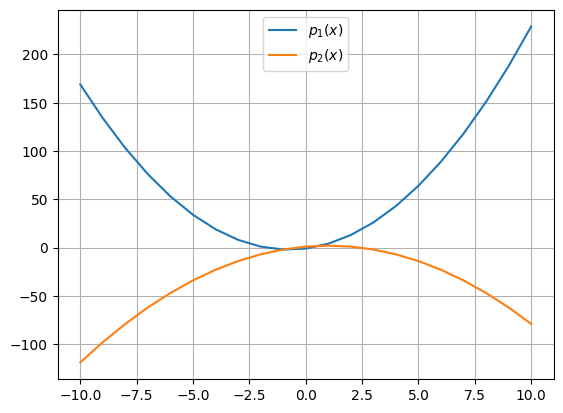
\includegraphics[keepaspectratio]{notebooks/22_funciones_y_docstring_files/figure-pdf/cell-43-output-1.png}}

\subsection{Ejemplo. Polinomios de cualquier
grado.}\label{ejemplo.-polinomios-de-cualquier-grado.}

Implementar una fábrica de polinomios de cualquier grado:

\[
\sum\limits_{k=0}^{n} a_k x^k = a_n x^n + a_{n-1} x^{n-1} + \dots + a_1 x + a_0 
\]

Probar con los siguientes polinomios: * \(p_0(x) = 5\) *
\(p_1(x) = 4 x + 2\) * \(p_2(x) = x^2 + 2x - 1\) *
\(p_3(x) = x^3 - x^2 + 3x\)

Graficar los polinomios como en el ejemplo 9.

\begin{Shaded}
\begin{Highlighting}[]
\KeywordTok{def}\NormalTok{ polFactory(}\OperatorTok{*}\NormalTok{coeficientes):}
    \CommentTok{"""}
\CommentTok{    Esta función construye y evalúa polinomios }
\CommentTok{    de cualquier grado.}

\CommentTok{    Parameters}
\CommentTok{    {-}{-}{-}{-}{-}{-}{-}{-}{-}{-}}
\CommentTok{    *coeficientes: coeficientes del polinomio a\_n, a\_\{n{-}1\}, ..., a\_0}
\CommentTok{    para construir el polinomio.}

\CommentTok{    Return}
\CommentTok{    {-}{-}{-}{-}{-}{-}}
\CommentTok{    Función que implementa el polinomio.}
\CommentTok{    """}
    
    \KeywordTok{def}\NormalTok{ polinomio(x):}
        \CommentTok{"""}
\CommentTok{        Función que implementa el polinomio y lo evalúa.}

\CommentTok{        Parameters}
\CommentTok{        {-}{-}{-}{-}{-}{-}{-}{-}{-}{-}}
\CommentTok{        x: valor para evaluar el polinomio.}

\CommentTok{        Return}
\CommentTok{        {-}{-}{-}{-}{-}{-}}
\CommentTok{        Resultado de evaluación del polinomio en \textquotesingle{}x\textquotesingle{}}
\CommentTok{        """}
\NormalTok{        res }\OperatorTok{=} \DecValTok{0}
        \ControlFlowTok{for}\NormalTok{ i, coef }\KeywordTok{in} \BuiltInTok{enumerate}\NormalTok{(coeficientes):}
\NormalTok{            res }\OperatorTok{+=}\NormalTok{ coef }\OperatorTok{*}\NormalTok{ x }\OperatorTok{**}\NormalTok{ i}
        \ControlFlowTok{return}\NormalTok{ res}
    
    \ControlFlowTok{return}\NormalTok{ polinomio}
\end{Highlighting}
\end{Shaded}

\begin{Shaded}
\begin{Highlighting}[]
\NormalTok{p1 }\OperatorTok{=}\NormalTok{ polFactory(}\DecValTok{5}\NormalTok{)}
\NormalTok{p2 }\OperatorTok{=}\NormalTok{ polFactory(}\DecValTok{1}\NormalTok{,}\DecValTok{2}\NormalTok{,}\DecValTok{3}\NormalTok{,}\DecValTok{4}\NormalTok{)}

\BuiltInTok{print}\NormalTok{(p1(}\FloatTok{3.1416}\NormalTok{))}
\BuiltInTok{print}\NormalTok{(p2(}\OperatorTok{{-}}\FloatTok{3.1416}\NormalTok{))}
\end{Highlighting}
\end{Shaded}

\begin{verbatim}
5.0
-99.700225117184
\end{verbatim}

\begin{Shaded}
\begin{Highlighting}[]
\CommentTok{\# Se generan 4 polinomios de diferente grado}
\NormalTok{p0 }\OperatorTok{=}\NormalTok{ polFactory(}\DecValTok{5}\NormalTok{)           }\CommentTok{\# 5.0}
\NormalTok{p1 }\OperatorTok{=}\NormalTok{ polFactory(}\DecValTok{2}\NormalTok{, }\DecValTok{4}\NormalTok{)        }\CommentTok{\# 4 x + 2}
\NormalTok{p2 }\OperatorTok{=}\NormalTok{ polFactory(}\OperatorTok{{-}}\DecValTok{1}\NormalTok{, }\DecValTok{2}\NormalTok{, }\DecValTok{1}\NormalTok{)    }\CommentTok{\# x\^{}2 + 2x {-} 1}
\NormalTok{p3 }\OperatorTok{=}\NormalTok{ polFactory(}\DecValTok{0}\NormalTok{, }\DecValTok{3}\NormalTok{, }\OperatorTok{{-}}\DecValTok{1}\NormalTok{, }\DecValTok{1}\NormalTok{) }\CommentTok{\# x\^{}3 {-} x\^{}2 + 3x + 0}

\CommentTok{\# Evaluación de los polinomios en el intervalo ({-}2,2) con pasos de 1}
\ControlFlowTok{for}\NormalTok{ x }\KeywordTok{in} \BuiltInTok{range}\NormalTok{(}\OperatorTok{{-}}\DecValTok{2}\NormalTok{, }\DecValTok{2}\NormalTok{):}
    \BuiltInTok{print}\NormalTok{(}\SpecialStringTok{f\textquotesingle{}x = }\SpecialCharTok{\{}\NormalTok{x}\SpecialCharTok{:3d\}}\SpecialStringTok{ }\CharTok{\textbackslash{}t}\SpecialStringTok{ p0(x) = }\SpecialCharTok{\{}\NormalTok{p0(x)}\SpecialCharTok{:3d\}}\SpecialStringTok{ }\CharTok{\textbackslash{}t}\SpecialStringTok{ p1(x) = }\SpecialCharTok{\{}\NormalTok{p1(x)}\SpecialCharTok{:3d\}}\SpecialStringTok{ }\CharTok{\textbackslash{}t}\SpecialStringTok{ p2(x) = }\SpecialCharTok{\{}\NormalTok{p2(x)}\SpecialCharTok{:3d\}}\SpecialStringTok{ }\CharTok{\textbackslash{}t}\SpecialStringTok{ p3(x) = }\SpecialCharTok{\{}\NormalTok{p3(x)}\SpecialCharTok{:3d\}}\SpecialStringTok{\textquotesingle{}}\NormalTok{)}
\end{Highlighting}
\end{Shaded}

\begin{verbatim}
x =  -2      p0(x) =   5     p1(x) =  -6     p2(x) =  -1     p3(x) = -18
x =  -1      p0(x) =   5     p1(x) =  -2     p2(x) =  -2     p3(x) =  -5
x =   0      p0(x) =   5     p1(x) =   2     p2(x) =  -1     p3(x) =   0
x =   1      p0(x) =   5     p1(x) =   6     p2(x) =   2     p3(x) =   3
\end{verbatim}

\begin{Shaded}
\begin{Highlighting}[]
\CommentTok{\# Graficación}
\NormalTok{x }\OperatorTok{=}\NormalTok{ []}
\NormalTok{p0\_v }\OperatorTok{=}\NormalTok{ []}
\NormalTok{p1\_v }\OperatorTok{=}\NormalTok{ []}
\NormalTok{p2\_v }\OperatorTok{=}\NormalTok{ []}
\NormalTok{p3\_v }\OperatorTok{=}\NormalTok{ []}

\ControlFlowTok{for}\NormalTok{ xi }\KeywordTok{in} \BuiltInTok{range}\NormalTok{(}\OperatorTok{{-}}\DecValTok{10}\NormalTok{, }\DecValTok{11}\NormalTok{):}
\NormalTok{    x.append(xi)}
\NormalTok{    p0\_v.append(p0(xi))}
\NormalTok{    p1\_v.append(p1(xi))}
\NormalTok{    p2\_v.append(p2(xi))}
\NormalTok{    p3\_v.append(p3(xi))}

\NormalTok{plt.plot(x, p0\_v, label}\OperatorTok{=}\StringTok{"$p\_0(x)$"}\NormalTok{)}
\NormalTok{plt.plot(x, p1\_v, label}\OperatorTok{=}\StringTok{"$p\_1(x)$"}\NormalTok{)}
\NormalTok{plt.plot(x, p2\_v, label}\OperatorTok{=}\StringTok{"$p\_2(x)$"}\NormalTok{)}
\NormalTok{plt.plot(x, p3\_v, label}\OperatorTok{=}\StringTok{"$p\_3(x)$"}\NormalTok{)}
\CommentTok{\#plt.ylim({-}200,200)}
\NormalTok{plt.grid()}
\NormalTok{plt.legend(loc}\OperatorTok{=}\StringTok{"upper center"}\NormalTok{, ncol}\OperatorTok{=}\DecValTok{2}\NormalTok{)}
\NormalTok{plt.show()}
\end{Highlighting}
\end{Shaded}

\pandocbounded{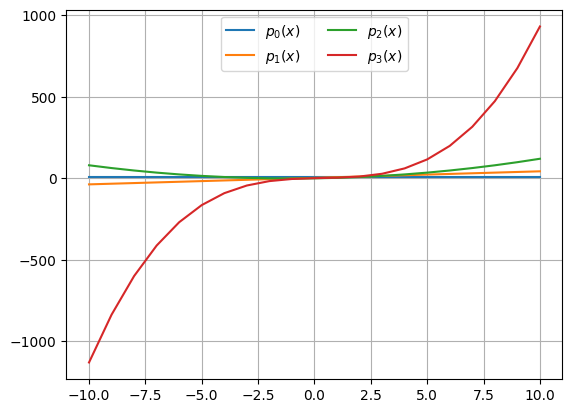
\includegraphics[keepaspectratio]{notebooks/22_funciones_y_docstring_files/figure-pdf/cell-47-output-1.png}}

\section{Ámbitos}\label{uxe1mbitos}

Algunos lenguajes como Python usan ámbitos (en algunos casos denominado
alcance) para definir variables (aunque también funciones y clases) de
tal manera que solo se puedan acceder desde cierto lugar y no desde
todas las ubicaciones de un programa.

En este caso, la capacidad para acceder a un nombre (de variable,
función o clase) dependerá de dónde se haya definido ese nombre.

\subsection{Local}\label{local}

Las funciones (y otros operadores también), crean su propio ámbito local
(\emph{scope}).

\begin{Shaded}
\begin{Highlighting}[]
\KeywordTok{def}\NormalTok{ actualizaEdad():}
\NormalTok{    edad }\OperatorTok{=} \DecValTok{21} \CommentTok{\# Variable local}
    \BuiltInTok{print}\NormalTok{(}\StringTok{"Ámbito de la función \textquotesingle{}actualizaEdad()\textquotesingle{}"}\NormalTok{)}
    \BuiltInTok{print}\NormalTok{(}\StringTok{"edad ="}\NormalTok{, edad, }\StringTok{", id(edad) ="}\NormalTok{, }\BuiltInTok{id}\NormalTok{(edad))}

\CommentTok{\# Ejecuto la función}
\NormalTok{actualizaEdad()}
\end{Highlighting}
\end{Shaded}

\begin{verbatim}
Ámbito de la función 'actualizaEdad()'
edad = 21 , id(edad) = 140714900203048
\end{verbatim}

\begin{Shaded}
\begin{Highlighting}[]
\CommentTok{\# ¿Se puede acceder al valor de \textquotesingle{}edad\textquotesingle{} fuera de la función?}
\BuiltInTok{print}\NormalTok{(}\StringTok{"Ámbito global: edad ="}\NormalTok{, edad, }\StringTok{", id(edad) ="}\NormalTok{, }\BuiltInTok{id}\NormalTok{(edad))}
\end{Highlighting}
\end{Shaded}

\begin{Highlighting}
\textcolor{black}{NameError: name 'edad' is not defined}
\textcolor{black}{}\textcolor{QuartoInternalColor1}{---------------------------------------------------------------------------}\textcolor{QuartoInternalColor2}{}
\textcolor{QuartoInternalColor2}{}\textcolor{QuartoInternalColor1}{NameError}\textcolor{QuartoInternalColor2}{                                 Traceback (most recent call last)}
\textcolor{QuartoInternalColor2}{}\textcolor{QuartoInternalColor3}{Cell}\textcolor{QuartoInternalColor2}{}\textcolor{QuartoInternalColor3}{ }\textcolor{QuartoInternalColor2}{}\textcolor{QuartoInternalColor4}{In[54]}\textcolor{QuartoInternalColor2}{}\textcolor{QuartoInternalColor4}{, line 2}\textcolor{QuartoInternalColor2}{}
\textcolor{QuartoInternalColor2}{}\textcolor{QuartoInternalColor4}{      1}\textcolor{QuartoInternalColor2}{ }\textcolor{QuartoInternalColor6}{# ¿Se puede acceder al valor de 'edad' fuera de la función?}\textcolor{QuartoInternalColor2}{}
\textcolor{QuartoInternalColor2}{}\textcolor{QuartoInternalColor4}{----> }\textcolor{QuartoInternalColor2}{}\textcolor{QuartoInternalColor4}{2}\textcolor{QuartoInternalColor2}{ }\textcolor{QuartoInternalColor5}{print}\textcolor{QuartoInternalColor2}{(}\textcolor{QuartoInternalColor7}{"}\textcolor{QuartoInternalColor2}{}\textcolor{QuartoInternalColor7}{Ámbito global: edad =}\textcolor{QuartoInternalColor2}{}\textcolor{QuartoInternalColor7}{"}\textcolor{QuartoInternalColor2}{, }\textcolor{QuartoInternalColor2}{edad}\textcolor{QuartoInternalColor2}{, }\textcolor{QuartoInternalColor7}{"}\textcolor{QuartoInternalColor2}{}\textcolor{QuartoInternalColor7}{, id(edad) =}\textcolor{QuartoInternalColor2}{}\textcolor{QuartoInternalColor7}{"}\textcolor{QuartoInternalColor2}{, }\textcolor{QuartoInternalColor5}{id}\textcolor{QuartoInternalColor2}{(edad))}
\textcolor{QuartoInternalColor2}{}\textcolor{QuartoInternalColor1}{NameError}\textcolor{QuartoInternalColor2}{: name 'edad' is not defined}
\end{Highlighting}

Se obtiene un error, pues \texttt{edad} solo está definida dentro del
ámbito local de la función \texttt{actualizaEdad()}.

\subsection{Global}\label{global}

El ámbito global es el alcance más alto en un programa, script o módulo
de Python. Este ámbito de Python contiene todos los nombres que se
definen en el nivel superior de un programa o módulo.

Los nombres en este ámbito son visibles desde cualquier lugar del
programa.

\begin{Shaded}
\begin{Highlighting}[]
\CommentTok{\# Variable creada en el ámbito global}
\NormalTok{edad }\OperatorTok{=} \DecValTok{25}
\end{Highlighting}
\end{Shaded}

\begin{Shaded}
\begin{Highlighting}[]
\BuiltInTok{print}\NormalTok{(}\StringTok{"Ámbito global: edad ="}\NormalTok{, edad, }\StringTok{", id(edad) ="}\NormalTok{, }\BuiltInTok{id}\NormalTok{(edad))}
\end{Highlighting}
\end{Shaded}

\begin{verbatim}
Ámbito global: edad = 25 , id(edad) = 140714900203176
\end{verbatim}

¿Qué pasa si ejectuamos nuevamente la función \texttt{actualizaEdad()}?

\begin{Shaded}
\begin{Highlighting}[]
\NormalTok{actualizaEdad()}
\end{Highlighting}
\end{Shaded}

\begin{verbatim}
Ámbito de la función 'actualizaEdad()'
edad = 21 , id(edad) = 140714900203048
\end{verbatim}

Observa que se usa la variable edad definida dentro de la función y es
diferente a la variable \texttt{edad} definida en el ámbito global.

Supongamos que deseamos incrementar el valor de la variable global
\texttt{edad} dentro de la función \texttt{actualizaEdad()} como sigue:

\begin{Shaded}
\begin{Highlighting}[]
\NormalTok{edad }\OperatorTok{=} \DecValTok{25}

\KeywordTok{def}\NormalTok{ actualizaEdad():}
\NormalTok{    edad }\OperatorTok{+=} \DecValTok{1}
    \ControlFlowTok{return}\NormalTok{ edad}

\NormalTok{actualizaEdad()}
\end{Highlighting}
\end{Shaded}

\begin{Highlighting}
\textcolor{black}{UnboundLocalError: cannot access local variable 'edad' where it is not associated with a value}
\textcolor{black}{}\textcolor{QuartoInternalColor1}{---------------------------------------------------------------------------}\textcolor{QuartoInternalColor2}{}
\textcolor{QuartoInternalColor2}{}\textcolor{QuartoInternalColor1}{UnboundLocalError}\textcolor{QuartoInternalColor2}{                         Traceback (most recent call last)}
\textcolor{QuartoInternalColor2}{}\textcolor{QuartoInternalColor3}{Cell}\textcolor{QuartoInternalColor2}{}\textcolor{QuartoInternalColor3}{ }\textcolor{QuartoInternalColor2}{}\textcolor{QuartoInternalColor4}{In[58]}\textcolor{QuartoInternalColor2}{}\textcolor{QuartoInternalColor4}{, line 7}\textcolor{QuartoInternalColor2}{}
\textcolor{QuartoInternalColor2}{}\textcolor{QuartoInternalColor4}{      4}\textcolor{QuartoInternalColor2}{     edad += }\textcolor{QuartoInternalColor4}{1}\textcolor{QuartoInternalColor2}{}
\textcolor{QuartoInternalColor2}{}\textcolor{QuartoInternalColor4}{      5}\textcolor{QuartoInternalColor2}{     }\textcolor{QuartoInternalColor5}{return}\textcolor{QuartoInternalColor2}{ edad}
\textcolor{QuartoInternalColor2}{}\textcolor{QuartoInternalColor4}{----> }\textcolor{QuartoInternalColor2}{}\textcolor{QuartoInternalColor4}{7}\textcolor{QuartoInternalColor2}{ }\textcolor{QuartoInternalColor2}{actualizaEdad}\textcolor{QuartoInternalColor2}{}\textcolor{QuartoInternalColor2}{(}\textcolor{QuartoInternalColor2}{}\textcolor{QuartoInternalColor2}{)}\textcolor{QuartoInternalColor2}{}
\textcolor{QuartoInternalColor2}{}\textcolor{QuartoInternalColor3}{Cell}\textcolor{QuartoInternalColor2}{}\textcolor{QuartoInternalColor3}{ }\textcolor{QuartoInternalColor2}{}\textcolor{QuartoInternalColor4}{In[58]}\textcolor{QuartoInternalColor2}{}\textcolor{QuartoInternalColor4}{, line 4}\textcolor{QuartoInternalColor2}{, in }\textcolor{QuartoInternalColor3}{actualizaEdad}\textcolor{QuartoInternalColor2}{}\textcolor{QuartoInternalColor8}{()}\textcolor{QuartoInternalColor2}{}
\textcolor{QuartoInternalColor2}{}\textcolor{QuartoInternalColor4}{      3}\textcolor{QuartoInternalColor2}{ }\textcolor{QuartoInternalColor5}{def}\textcolor{QuartoInternalColor2}{}\textcolor{QuartoInternalColor9}{ }\textcolor{QuartoInternalColor2}{}\textcolor{QuartoInternalColor8}{actualizaEdad}\textcolor{QuartoInternalColor2}{():}
\textcolor{QuartoInternalColor2}{}\textcolor{QuartoInternalColor4}{----> }\textcolor{QuartoInternalColor2}{}\textcolor{QuartoInternalColor4}{4}\textcolor{QuartoInternalColor2}{     }\textcolor{QuartoInternalColor2}{edad}\textcolor{QuartoInternalColor2}{ += }\textcolor{QuartoInternalColor4}{1}\textcolor{QuartoInternalColor2}{}
\textcolor{QuartoInternalColor2}{}\textcolor{QuartoInternalColor4}{      5}\textcolor{QuartoInternalColor2}{     }\textcolor{QuartoInternalColor5}{return}\textcolor{QuartoInternalColor2}{ edad}
\textcolor{QuartoInternalColor2}{}\textcolor{QuartoInternalColor1}{UnboundLocalError}\textcolor{QuartoInternalColor2}{: cannot access local variable 'edad' where it is not associated with a value}
\end{Highlighting}

Observa que se genera un error de tipo \texttt{UnboundLocalError} porque
se está intentando acceder a un nombre que aún no está definido en el
ámbito local de la función.

Entonces, para hacer referencia a la variable global \texttt{edad} y
modificarla dentro de la función, debes usar la declaración
\texttt{global}:

\begin{Shaded}
\begin{Highlighting}[]
\NormalTok{edad }\OperatorTok{=} \DecValTok{25}

\KeywordTok{def}\NormalTok{ actualizaEdad():}
    \KeywordTok{global}\NormalTok{ edad}
\NormalTok{    edad }\OperatorTok{+=} \DecValTok{1}
    \ControlFlowTok{return}\NormalTok{ edad}

\NormalTok{actualizaEdad()}
\end{Highlighting}
\end{Shaded}

\begin{verbatim}
26
\end{verbatim}

Aunque lo anterior funciona correctamente, no es recomendable usar esta
solución, pues puede tener efectos no deseables.

Una mejor solución sería la siguiente:

\begin{Shaded}
\begin{Highlighting}[]
\NormalTok{edad }\OperatorTok{=} \DecValTok{25}

\KeywordTok{def}\NormalTok{ actualizaEdad(e):}
    \ControlFlowTok{return}\NormalTok{ e }\OperatorTok{+} \DecValTok{1}

\NormalTok{edad }\OperatorTok{=}\NormalTok{ actualizaEdad(edad)}

\BuiltInTok{print}\NormalTok{(edad)}
\end{Highlighting}
\end{Shaded}

\begin{verbatim}
26
\end{verbatim}

\subsection{\texorpdfstring{Enclosing
(\emph{nonlocal})}{Enclosing (nonlocal)}}\label{enclosing-nonlocal}

El ámbito \emph{enclosing} es un alcance especial que solo existe para
funciones anidadas.

\begin{Shaded}
\begin{Highlighting}[]
\KeywordTok{def}\NormalTok{ datosPersonales():}
\NormalTok{    edad }\OperatorTok{=} \DecValTok{25}

    \KeywordTok{def}\NormalTok{ actualizaEdad():}
        \BuiltInTok{print}\NormalTok{(edad)}

\NormalTok{    actualizaEdad()}

\NormalTok{datosPersonales()}
\end{Highlighting}
\end{Shaded}

\begin{verbatim}
25
\end{verbatim}

Es posible acceder a las variables definidas en el ámbito de la función
\texttt{datosPersonales()} (\emph{Enclosing scope}) desde funciones
internas o anidadas como \texttt{actualizaEdad()}.

Pero no es posible modificar las variables, checa el siguiente código:

\begin{Shaded}
\begin{Highlighting}[]
\KeywordTok{def}\NormalTok{ datosPersonales():}
\NormalTok{    edad }\OperatorTok{=} \DecValTok{25}

    \KeywordTok{def}\NormalTok{ actualizaEdad():}
\NormalTok{        edad }\OperatorTok{+=} \DecValTok{1}
        \ControlFlowTok{return}\NormalTok{ edad}

\NormalTok{    actualizaEdad()}

    \ControlFlowTok{return}\NormalTok{ edad}

\NormalTok{datosPersonales()}
\end{Highlighting}
\end{Shaded}

\begin{Highlighting}
\textcolor{black}{UnboundLocalError: cannot access local variable 'edad' where it is not associated with a value}
\textcolor{black}{}\textcolor{QuartoInternalColor1}{---------------------------------------------------------------------------}\textcolor{QuartoInternalColor2}{}
\textcolor{QuartoInternalColor2}{}\textcolor{QuartoInternalColor1}{UnboundLocalError}\textcolor{QuartoInternalColor2}{                         Traceback (most recent call last)}
\textcolor{QuartoInternalColor2}{}\textcolor{QuartoInternalColor3}{Cell}\textcolor{QuartoInternalColor2}{}\textcolor{QuartoInternalColor3}{ }\textcolor{QuartoInternalColor2}{}\textcolor{QuartoInternalColor4}{In[62]}\textcolor{QuartoInternalColor2}{}\textcolor{QuartoInternalColor4}{, line 12}\textcolor{QuartoInternalColor2}{}
\textcolor{QuartoInternalColor2}{}\textcolor{QuartoInternalColor4}{      8}\textcolor{QuartoInternalColor2}{     actualizaEdad()}
\textcolor{QuartoInternalColor2}{}\textcolor{QuartoInternalColor4}{     10}\textcolor{QuartoInternalColor2}{     }\textcolor{QuartoInternalColor5}{return}\textcolor{QuartoInternalColor2}{ edad}
\textcolor{QuartoInternalColor2}{}\textcolor{QuartoInternalColor4}{---> }\textcolor{QuartoInternalColor2}{}\textcolor{QuartoInternalColor4}{12}\textcolor{QuartoInternalColor2}{ }\textcolor{QuartoInternalColor2}{datosPersonales}\textcolor{QuartoInternalColor2}{}\textcolor{QuartoInternalColor2}{(}\textcolor{QuartoInternalColor2}{}\textcolor{QuartoInternalColor2}{)}\textcolor{QuartoInternalColor2}{}
\textcolor{QuartoInternalColor2}{}\textcolor{QuartoInternalColor3}{Cell}\textcolor{QuartoInternalColor2}{}\textcolor{QuartoInternalColor3}{ }\textcolor{QuartoInternalColor2}{}\textcolor{QuartoInternalColor4}{In[62]}\textcolor{QuartoInternalColor2}{}\textcolor{QuartoInternalColor4}{, line 8}\textcolor{QuartoInternalColor2}{, in }\textcolor{QuartoInternalColor3}{datosPersonales}\textcolor{QuartoInternalColor2}{}\textcolor{QuartoInternalColor8}{()}\textcolor{QuartoInternalColor2}{}
\textcolor{QuartoInternalColor2}{}\textcolor{QuartoInternalColor4}{      5}\textcolor{QuartoInternalColor2}{     edad += }\textcolor{QuartoInternalColor4}{1}\textcolor{QuartoInternalColor2}{}
\textcolor{QuartoInternalColor2}{}\textcolor{QuartoInternalColor4}{      6}\textcolor{QuartoInternalColor2}{     }\textcolor{QuartoInternalColor5}{return}\textcolor{QuartoInternalColor2}{ edad}
\textcolor{QuartoInternalColor2}{}\textcolor{QuartoInternalColor4}{----> }\textcolor{QuartoInternalColor2}{}\textcolor{QuartoInternalColor4}{8}\textcolor{QuartoInternalColor2}{ }\textcolor{QuartoInternalColor2}{actualizaEdad}\textcolor{QuartoInternalColor2}{}\textcolor{QuartoInternalColor2}{(}\textcolor{QuartoInternalColor2}{}\textcolor{QuartoInternalColor2}{)}\textcolor{QuartoInternalColor2}{}
\textcolor{QuartoInternalColor2}{}\textcolor{QuartoInternalColor4}{     10}\textcolor{QuartoInternalColor2}{ }\textcolor{QuartoInternalColor5}{return}\textcolor{QuartoInternalColor2}{ edad}
\textcolor{QuartoInternalColor2}{}\textcolor{QuartoInternalColor3}{Cell}\textcolor{QuartoInternalColor2}{}\textcolor{QuartoInternalColor3}{ }\textcolor{QuartoInternalColor2}{}\textcolor{QuartoInternalColor4}{In[62]}\textcolor{QuartoInternalColor2}{}\textcolor{QuartoInternalColor4}{, line 5}\textcolor{QuartoInternalColor2}{, in }\textcolor{QuartoInternalColor3}{datosPersonales.<locals>.actualizaEdad}\textcolor{QuartoInternalColor2}{}\textcolor{QuartoInternalColor8}{()}\textcolor{QuartoInternalColor2}{}
\textcolor{QuartoInternalColor2}{}\textcolor{QuartoInternalColor4}{      4}\textcolor{QuartoInternalColor2}{ }\textcolor{QuartoInternalColor5}{def}\textcolor{QuartoInternalColor2}{}\textcolor{QuartoInternalColor9}{ }\textcolor{QuartoInternalColor2}{}\textcolor{QuartoInternalColor8}{actualizaEdad}\textcolor{QuartoInternalColor2}{():}
\textcolor{QuartoInternalColor2}{}\textcolor{QuartoInternalColor4}{----> }\textcolor{QuartoInternalColor2}{}\textcolor{QuartoInternalColor4}{5}\textcolor{QuartoInternalColor2}{     }\textcolor{QuartoInternalColor2}{edad}\textcolor{QuartoInternalColor2}{ += }\textcolor{QuartoInternalColor4}{1}\textcolor{QuartoInternalColor2}{}
\textcolor{QuartoInternalColor2}{}\textcolor{QuartoInternalColor4}{      6}\textcolor{QuartoInternalColor2}{     }\textcolor{QuartoInternalColor5}{return}\textcolor{QuartoInternalColor2}{ edad}
\textcolor{QuartoInternalColor2}{}\textcolor{QuartoInternalColor1}{UnboundLocalError}\textcolor{QuartoInternalColor2}{: cannot access local variable 'edad' where it is not associated with a value}
\end{Highlighting}

Observa que se obtiene otro error de tipo \texttt{UnboundLocalError},
pues estamos intentando actualizar la variable \texttt{edad} definida en
el ámbito de la función \texttt{datosPersonales()}.

Para resolver este problema podemos usar la declaración
\texttt{nonlocal}:

\begin{Shaded}
\begin{Highlighting}[]
\KeywordTok{def}\NormalTok{ datosPersonales():}
\NormalTok{    edad }\OperatorTok{=} \DecValTok{25}

    \KeywordTok{def}\NormalTok{ actualizaEdad():}
        \KeywordTok{nonlocal}\NormalTok{ edad}
\NormalTok{        edad }\OperatorTok{+=} \DecValTok{1}
        \ControlFlowTok{return}\NormalTok{ edad}

\NormalTok{    actualizaEdad()}

    \ControlFlowTok{return}\NormalTok{ edad}

\NormalTok{datosPersonales()}
\end{Highlighting}
\end{Shaded}

\begin{verbatim}
26
\end{verbatim}

\subsection{Built-in}\label{built-in}

Es un ámbito especial de Python que se crea cada vez que se ejecuta un
código o se abre una sesión interactiva.

Este ámbito contiene nombres como palabras clave, funciones, excepciones
y otros atributos incorporados en Python.

Los nombres en este ámbito están disponibles en todas partes del código.

\section{\texorpdfstring{Documentación con
\emph{docstring}}{Documentación con docstring}}\label{documentaciuxf3n-con-docstring}

Python ofrece dos tipos básicos de comentarios para documentar el
código:

\begin{enumerate}
\def\labelenumi{\arabic{enumi}.}
\tightlist
\item
  Lineal. Este tipo de comentarios se llevan a cabo utilizando el
  símbolo especial \texttt{\#}. El intérprete de Python sabrá que todo
  lo que sigue delante de este símbolo es un comentario y por lo tanto
  no se toma en cuenta en la ejecución:
\end{enumerate}

\begin{Shaded}
\begin{Highlighting}[]
\NormalTok{a }\OperatorTok{=} \DecValTok{10} \CommentTok{\# Este es un comentario}
\end{Highlighting}
\end{Shaded}

\begin{enumerate}
\def\labelenumi{\arabic{enumi}.}
\setcounter{enumi}{1}
\tightlist
\item
  Docstrings En programación, un \emph{docstring} es una cadena de
  caracteres embedidas en el código fuente, similares a un comentario,
  para documentar un segmento de código específico. A diferencia de los
  comentarios tradicionales, las docstrings no se quitan del código
  cuando es analizado, sino que son retenidas a través de la ejecución
  del programa. Esto permite al programador inspeccionar esos
  comentarios en tiempo de ejecución, por ejemplo como un sistema de
  ayuda interactivo o como metadatos. En Python se utilizan las triples
  comillas para definir un \emph{docstring}.
\end{enumerate}

\begin{Shaded}
\begin{Highlighting}[]
\KeywordTok{def}\NormalTok{ funcion(x):}
    \CommentTok{\textquotesingle{}\textquotesingle{}\textquotesingle{}}
\CommentTok{    Esta es una descripción de la función ...}
\CommentTok{    \textquotesingle{}\textquotesingle{}\textquotesingle{}}
    
\KeywordTok{def}\NormalTok{ foo(y):}
    \CommentTok{"""}
\CommentTok{    También de esta manera se puede definir una docstring}
\CommentTok{    """}
   
\end{Highlighting}
\end{Shaded}

\begin{Shaded}
\begin{Highlighting}[]
\KeywordTok{def}\NormalTok{ suma(a,b):}
    \CommentTok{\textquotesingle{}\textquotesingle{}\textquotesingle{}}
\CommentTok{    Esta función calcula  la suma de los parámetros a y b. }
\CommentTok{    Regresa el resultado de la suma}
\CommentTok{    \textquotesingle{}\textquotesingle{}\textquotesingle{}}
    \ControlFlowTok{return}\NormalTok{ a }\OperatorTok{+}\NormalTok{ b}
\end{Highlighting}
\end{Shaded}

\begin{Shaded}
\begin{Highlighting}[]
\NormalTok{suma}
\end{Highlighting}
\end{Shaded}

\begin{verbatim}
<function __main__.suma(a, b)>
\end{verbatim}

\begin{Shaded}
\begin{Highlighting}[]
\CommentTok{\# En numpy se usa la siguiente definición de docstrings}
\KeywordTok{def}\NormalTok{ suma(a,b):}
    \CommentTok{\textquotesingle{}\textquotesingle{}\textquotesingle{}}
\CommentTok{    Calcula la suma de los dos parámetros a y b.}
\CommentTok{    }
\CommentTok{    Args: }
\CommentTok{        a: int Numero a sumar}
\CommentTok{        b: int Numero a sumar}
\CommentTok{    Return:}
\CommentTok{        c: int Suma del numero a y b}
\CommentTok{    \textquotesingle{}\textquotesingle{}\textquotesingle{}}
\NormalTok{    c }\OperatorTok{=}\NormalTok{ a }\OperatorTok{+}\NormalTok{ b}
    \ControlFlowTok{return}\NormalTok{ c}
\end{Highlighting}
\end{Shaded}

\begin{Shaded}
\begin{Highlighting}[]
\NormalTok{suma}
\end{Highlighting}
\end{Shaded}

Existen diferentes estilos de documentación tipo \emph{docstring} vease
por ejemplo:

\begin{itemize}
\tightlist
\item
  Numpy,
\item
  Matplotlib.
\end{itemize}

Para más información véase PEP 257 -- Docstring Conventions y PEP 8 --
Style Guide for Python Code.

\bookmarksetup{startatroot}

\chapter{Importando bibliotecas.}\label{sec-import}

\textbf{Objetivo.} Mostrar como importar módulos de la biblioteca
estándar y algunos ejemplos de su uso.

\section{La biblioteca estándar de
Python.}\label{sec-biblioteca_estandar}

La \textbf{biblioteca estándar} de Python está compuesta por módulos con
funcionalidades adicionales y que se distribuyen con la instalación de
básica del lenguaje, por lo que no es necesaria una instalación
adicional. El conjunto de funciones y herramientas de esta biblioteca es
muy extensa y ofrece una amplia gama de aplicaciones.

Estos módulos o bibliotecas permiten, entre otras cosas, tener una
interfaz con el sistema operativo, manejo de archivos, medición de
tiempos, fechas, matemáticas y pruebas unitarias.

La forma de incorporar y usar de estas herramientas es simple y
estándar. En esta notebook veremos algunos ejemplos.

\section{Importando las bibliotecas.}\label{sec-import}

Las bibliotecas se pueden de importar varias formas:

\textbf{1. Importando usando el nombre:}

\begin{verbatim}
import nombre_de_la_biblioteca
\end{verbatim}

En este caso, para usar una función se debe anteponer el nombre completo
de la biblioteca:

\begin{verbatim}
nombre_de_la_biblioteca.funcion_x()
\end{verbatim}

\textbf{2. Importando usando el nombre y un alias:}

\begin{verbatim}
import nombre_de_la_biblioteca as nb
\end{verbatim}

En este caso, para usar una función se debe anteponer el alias de la
biblioteca:

\begin{verbatim}
nb.funcion_x()
\end{verbatim}

\textbf{3. Importando todas las funciones de la biblioteca con
\texttt{*}:}

\begin{verbatim}
from nombre_de_la_biblioteca import *
\end{verbatim}

En este caso, para usar una función se puede usar el nombre de la misma
sin anteponer nada:

\begin{verbatim}
funcion_x()
\end{verbatim}

\textbf{4. Importando solo una función de la biblioteca :}

\begin{verbatim}
from nombre_de_la_biblioteca import funcion_x
\end{verbatim}

En este caso, para usar la función solo es necesario el nombre de la
misma:

\begin{verbatim}
funcion_x()
\end{verbatim}

Por cada función que se requiera, se debe agregar el nombre en la
importación separada por coma:

\begin{verbatim}
from nombre_de_la_biblioteca import funcion_x, funcion_y
\end{verbatim}

\textbf{5. Importando solo una función de la biblioteca y un alias:}

\begin{verbatim}
from nombre_de_la_biblioteca import funcion_x as fx
\end{verbatim}

En este caso, para usar la función se usa el alias \texttt{fx} y se
puede ejecutar como sigue:

\begin{verbatim}
fx()
\end{verbatim}

\section{Funciones matemáticas.}\label{sec-funciones_math}

\subsection{\texorpdfstring{\texttt{math} y
\texttt{cmath}}{math y cmath}}\label{math-y-cmath}

\begin{itemize}
\item
  El módulo \texttt{math} provee de las funciones matemáticas definida
  en la biblioteca estándar de C para números \textbf{reales}. Más
  información en math.
\item
  El módulo \texttt{cmath} provee de las funciones matemáticas para
  números \textbf{complejos}. Más información en cmath.
\end{itemize}

\begin{Shaded}
\begin{Highlighting}[]
\ImportTok{import}\NormalTok{ math}
\BuiltInTok{print}\NormalTok{(math.sqrt(}\DecValTok{4}\NormalTok{))}
\BuiltInTok{print}\NormalTok{(math.pi)}
\BuiltInTok{print}\NormalTok{(math.sin(math.pi }\OperatorTok{/} \DecValTok{2}\NormalTok{))}
\BuiltInTok{print}\NormalTok{(math.cos(}\DecValTok{0}\NormalTok{))}
\end{Highlighting}
\end{Shaded}

\begin{verbatim}
2.0
3.141592653589793
1.0
1.0
\end{verbatim}

\begin{Shaded}
\begin{Highlighting}[]
\ImportTok{import}\NormalTok{ cmath}

\NormalTok{complejo }\OperatorTok{=} \DecValTok{1} \OperatorTok{+} \OtherTok{4j}
\BuiltInTok{print}\NormalTok{(complejo)}
\BuiltInTok{print}\NormalTok{(cmath.sin(complejo))}
\end{Highlighting}
\end{Shaded}

\begin{verbatim}
(1+4j)
(22.979085577886128+14.744805188558727j)
\end{verbatim}

\subsection{\texorpdfstring{\texttt{random}}{random}}\label{random}

Este módulo implementa generadores de números pseudoaleatorios para
varias distribuciones. Más información en random.

\begin{Shaded}
\begin{Highlighting}[]
\ImportTok{import}\NormalTok{ random}

\CommentTok{\# randint(): Elige un número entre 0 y 5}
\BuiltInTok{print}\NormalTok{(random.randint(}\DecValTok{0}\NormalTok{, }\DecValTok{5}\NormalTok{))}

\CommentTok{\# random(): Genera un número entre 0 y 1}
\BuiltInTok{print}\NormalTok{(random.random())}

\CommentTok{\# choice(): Selecciona entre varios elementos de una secuencia}
\NormalTok{myList }\OperatorTok{=}\NormalTok{ [}\DecValTok{2}\NormalTok{, }\DecValTok{109}\NormalTok{, }\VariableTok{False}\NormalTok{, }\DecValTok{10}\NormalTok{, }\StringTok{"Lorem"}\NormalTok{, }\DecValTok{482}\NormalTok{, }\StringTok{"Ipsum"}\NormalTok{]}
\BuiltInTok{print}\NormalTok{(random.choice(myList))}

\CommentTok{\# suffle(): Ordena una lista de manera pseudoaleatoria}
\NormalTok{x }\OperatorTok{=}\NormalTok{ [[i] }\ControlFlowTok{for}\NormalTok{ i }\KeywordTok{in} \BuiltInTok{range}\NormalTok{(}\DecValTok{10}\NormalTok{)]}
\NormalTok{random.shuffle(x)}
\BuiltInTok{print}\NormalTok{(x)}

\CommentTok{\# randrange(): Elige un valor en un rango}
\ControlFlowTok{for}\NormalTok{ i }\KeywordTok{in} \BuiltInTok{range}\NormalTok{(}\DecValTok{3}\NormalTok{):}
    \BuiltInTok{print}\NormalTok{(random.randrange(}\DecValTok{0}\NormalTok{, }\DecValTok{101}\NormalTok{, }\DecValTok{5}\NormalTok{))}
\end{Highlighting}
\end{Shaded}

\begin{verbatim}
4
0.5825953813963569
482
[[5], [8], [7], [3], [2], [6], [9], [4], [1], [0]]
25
5
0
\end{verbatim}

\subsection{\texorpdfstring{\texttt{statistics}}{statistics}}\label{statistics}

Este módulo proporciona funciones para calcular estadísticas matemáticas
de datos numéricos (valores reales). Más información en statistics.

\begin{Shaded}
\begin{Highlighting}[]
\ImportTok{import}\NormalTok{ statistics}

\NormalTok{example\_list }\OperatorTok{=}\NormalTok{ [}\DecValTok{5}\NormalTok{,}\DecValTok{2}\NormalTok{,}\DecValTok{5}\NormalTok{,}\DecValTok{6}\NormalTok{,}\DecValTok{1}\NormalTok{,}\DecValTok{2}\NormalTok{,}\DecValTok{6}\NormalTok{,}\DecValTok{7}\NormalTok{,}\DecValTok{2}\NormalTok{,}\DecValTok{6}\NormalTok{,}\DecValTok{3}\NormalTok{,}\DecValTok{5}\NormalTok{,}\DecValTok{5}\NormalTok{]}

\NormalTok{x }\OperatorTok{=}\NormalTok{ statistics.mean(example\_list)}
\BuiltInTok{print}\NormalTok{(x)}

\NormalTok{y }\OperatorTok{=}\NormalTok{ statistics.median(example\_list)}
\BuiltInTok{print}\NormalTok{(y)}

\NormalTok{z }\OperatorTok{=}\NormalTok{ statistics.mode(example\_list)}
\BuiltInTok{print}\NormalTok{(z)}

\NormalTok{a }\OperatorTok{=}\NormalTok{ statistics.stdev(example\_list)}
\BuiltInTok{print}\NormalTok{(a)}

\NormalTok{b }\OperatorTok{=}\NormalTok{ statistics.variance(example\_list)}
\BuiltInTok{print}\NormalTok{(b)}
\end{Highlighting}
\end{Shaded}

\begin{verbatim}
4.230769230769231
5
5
1.9644272343292228
3.858974358974359
\end{verbatim}

\section{Sistema operativo.}\label{sec-bib_sistema}

\subsection{\texorpdfstring{\texttt{os}}{os}}\label{os}

Este módulo provee una manera portable de interactuar con el sistema
operativo. Más información en os.

Se puede por ejemplo, crear, eliminar y mover carpetas/archivos,
cambiarse de directorio, acceder a los nombres de archivos dentro de una
ruta, etc.

\begin{Shaded}
\begin{Highlighting}[]
\ImportTok{import}\NormalTok{ os}

\NormalTok{directorio\_actual }\OperatorTok{=}\NormalTok{ os.getcwd()}
\BuiltInTok{print}\NormalTok{(directorio\_actual)}
\end{Highlighting}
\end{Shaded}

\begin{verbatim}
C:\Users\luiggi\Documents\GitSites\introduccion_python\notebooks
\end{verbatim}

\begin{Shaded}
\begin{Highlighting}[]
\NormalTok{os.mkdir(}\StringTok{\textquotesingle{}nueva\_carpeta\textquotesingle{}}\NormalTok{)}
\end{Highlighting}
\end{Shaded}

\begin{Shaded}
\begin{Highlighting}[]
\NormalTok{os.chdir(}\StringTok{\textquotesingle{}nueva\_carpeta\textquotesingle{}}\NormalTok{)}
\end{Highlighting}
\end{Shaded}

\begin{Shaded}
\begin{Highlighting}[]
\BuiltInTok{print}\NormalTok{(os.getcwd())}
\end{Highlighting}
\end{Shaded}

\begin{verbatim}
C:\Users\luiggi\Documents\GitSites\introduccion_python\notebooks\nueva_carpeta
\end{verbatim}

\begin{Shaded}
\begin{Highlighting}[]
\NormalTok{os.chdir(}\StringTok{\textquotesingle{}../\textquotesingle{}}\NormalTok{)}
\end{Highlighting}
\end{Shaded}

\begin{Shaded}
\begin{Highlighting}[]
\BuiltInTok{print}\NormalTok{(os.getcwd())}
\end{Highlighting}
\end{Shaded}

\begin{verbatim}
C:\Users\luiggi\Documents\GitSites\introduccion_python\notebooks
\end{verbatim}

\begin{Shaded}
\begin{Highlighting}[]
\NormalTok{os.rename(}\StringTok{\textquotesingle{}nueva\_carpeta\textquotesingle{}}\NormalTok{,}\StringTok{\textquotesingle{}nueva\textquotesingle{}}\NormalTok{)}
\end{Highlighting}
\end{Shaded}

\begin{Shaded}
\begin{Highlighting}[]
\NormalTok{os.listdir()}
\end{Highlighting}
\end{Shaded}

\begin{verbatim}
['.ipynb_checkpoints',
 '01_variables_objetos.ipynb',
 '01_variables_objetos_files',
 '02_tipos_basicos.ipynb',
 '02_tipos_basicos_files',
 '03_operadores.ipynb',
 '04_expresiones_declaraciones.ipynb',
 '05_cadenas.ipynb',
 '06_input.ipynb',
 '07_archivos.ipynb',
 '08_control_de_flujo.ipynb',
 '09_listas.ipynb',
 '10_tuplas.ipynb',
 '11_conjuntos.ipynb',
 '12_diccionarios.ipynb',
 '13_ds_casting.ipynb',
 '14_ds_traversing.ipynb',
 '15_funciones.ipynb',
 '16_excepciones_files',
 '16_lambda_expressions.ipynb',
 '17_excepciones.ipynb',
 '18_comprehensions.ipynb',
 '19_iterables_map_filter_reduce.ipynb',
 '20_decoradores.ipynb',
 '21_iteradores_generadores.ipynb',
 '22_funciones_y_docstring.ipynb',
 '23_import.ipynb',
 '23_import_files',
 'contexto_ejemplo',
 'gatitos.txt',
 'gatos.txt',
 'mi_archivo.txt',
 'nombres.txt',
 'nueva',
 'poema20.txt',
 'QueLesQuedaALosJovenes.txt',
 'Untitled.ipynb']
\end{verbatim}

\begin{Shaded}
\begin{Highlighting}[]
\NormalTok{os.rmdir(}\StringTok{\textquotesingle{}nueva\textquotesingle{}}\NormalTok{)}
\end{Highlighting}
\end{Shaded}

\begin{Shaded}
\begin{Highlighting}[]
\NormalTok{os.listdir()}
\end{Highlighting}
\end{Shaded}

\begin{verbatim}
['.ipynb_checkpoints',
 '01_variables_objetos.ipynb',
 '01_variables_objetos_files',
 '02_tipos_basicos.ipynb',
 '02_tipos_basicos_files',
 '03_operadores.ipynb',
 '04_expresiones_declaraciones.ipynb',
 '05_cadenas.ipynb',
 '06_input.ipynb',
 '07_archivos.ipynb',
 '08_control_de_flujo.ipynb',
 '09_listas.ipynb',
 '10_tuplas.ipynb',
 '11_conjuntos.ipynb',
 '12_diccionarios.ipynb',
 '13_ds_casting.ipynb',
 '14_ds_traversing.ipynb',
 '15_funciones.ipynb',
 '16_excepciones_files',
 '16_lambda_expressions.ipynb',
 '17_excepciones.ipynb',
 '18_comprehensions.ipynb',
 '19_iterables_map_filter_reduce.ipynb',
 '20_decoradores.ipynb',
 '21_iteradores_generadores.ipynb',
 '22_funciones_y_docstring.ipynb',
 '23_import.ipynb',
 '23_import_files',
 'contexto_ejemplo',
 'gatitos.txt',
 'gatos.txt',
 'mi_archivo.txt',
 'nombres.txt',
 'poema20.txt',
 'QueLesQuedaALosJovenes.txt',
 'Untitled.ipynb']
\end{verbatim}

\subsection{\texorpdfstring{\texttt{platform}}{platform}}\label{platform}

Para acceso a los datos identificativos de la plataforma subyacente. Más
información en platform.

\begin{Shaded}
\begin{Highlighting}[]
\ImportTok{import}\NormalTok{ platform}

\NormalTok{SO }\OperatorTok{=}\NormalTok{ platform.system()}

\ControlFlowTok{if}\NormalTok{ SO }\OperatorTok{==} \StringTok{"Windows"}\NormalTok{:}
    \BuiltInTok{print}\NormalTok{(}\StringTok{"Sistema operativo : Windows 11"}\NormalTok{)}
\ControlFlowTok{elif}\NormalTok{ SO }\OperatorTok{==} \StringTok{"Linux"}\NormalTok{:}
    \BuiltInTok{print}\NormalTok{(}\StringTok{"Sistema operativo : Linux 11"}\NormalTok{)}
\ControlFlowTok{elif}\NormalTok{ SO }\OperatorTok{==} \StringTok{"Darwin"}\NormalTok{:}
    \BuiltInTok{print}\NormalTok{(}\StringTok{"Sistema operativo : MacOS"}\NormalTok{)}
\end{Highlighting}
\end{Shaded}

\begin{verbatim}
Sistema operativo : Windows 11
\end{verbatim}

\subsection{\texorpdfstring{\texttt{shutil}}{shutil}}\label{shutil}

El módulo \texttt{shutil} ofrece una serie de operaciones de alto nivel
en archivos y colecciones de archivos. En particular, se proporcionan
funciones que admiten la copia y eliminación de archivos. Más
información en shutil.

\begin{Shaded}
\begin{Highlighting}[]
\ImportTok{import}\NormalTok{ os, shutil}

\CommentTok{\# Obtenemos el directorio original}
\NormalTok{dir\_original }\OperatorTok{=}\NormalTok{ os.getcwd()}

\CommentTok{\# Obtenemos la lista de archivos}
\NormalTok{lista\_archivos }\OperatorTok{=}\NormalTok{ os.listdir(dir\_original)}

\CommentTok{\# Creamos una carpeta}
\NormalTok{os.mkdir(}\StringTok{\textquotesingle{}BORRAME\textquotesingle{}}\NormalTok{)}

\CommentTok{\# Creamos una cadena con la ruta a la nueva carpeta}
\NormalTok{dir\_destino }\OperatorTok{=}\NormalTok{ os.path.join(dir\_original, }\StringTok{\textquotesingle{}BORRAME\textquotesingle{}}\NormalTok{)}
\BuiltInTok{print}\NormalTok{(}\StringTok{"Ruta:"}\NormalTok{, dir\_destino)}

\CommentTok{\# Recorremos la lista de archivos}
\ControlFlowTok{for}\NormalTok{ files }\KeywordTok{in}\NormalTok{ lista\_archivos:}
    \CommentTok{\# Si el nombre termina con ".txt" lo copiamos a la carpeta}
    \ControlFlowTok{if}\NormalTok{ files.endswith(}\StringTok{".txt"}\NormalTok{):}
\NormalTok{        shutil.copy(files, dir\_destino)}
        
\CommentTok{\# Listamos los archivos en la carpeta}
\NormalTok{os.listdir(}\StringTok{\textquotesingle{}./BORRAME/\textquotesingle{}}\NormalTok{)}
\end{Highlighting}
\end{Shaded}

\begin{verbatim}
Ruta: C:\Users\luiggi\Documents\GitSites\introduccion_python\notebooks\BORRAME
\end{verbatim}

\begin{verbatim}
['gatitos.txt',
 'gatos.txt',
 'mi_archivo.txt',
 'nombres.txt',
 'poema20.txt',
 'QueLesQuedaALosJovenes.txt']
\end{verbatim}

\begin{Shaded}
\begin{Highlighting}[]
\CommentTok{\# Eliminamos la carpeta}
\NormalTok{shutil.rmtree(}\StringTok{"./BORRAME/"}\NormalTok{)}
\end{Highlighting}
\end{Shaded}

\subsection{\texorpdfstring{\texttt{sys}}{sys}}\label{sys}

Provee información acerca de las constantes, funciones y métodos del
interprete de Python. Más información en sys.

\begin{Shaded}
\begin{Highlighting}[]
\ImportTok{import}\NormalTok{ sys}
\end{Highlighting}
\end{Shaded}

\begin{Shaded}
\begin{Highlighting}[]
\NormalTok{sys.version}
\end{Highlighting}
\end{Shaded}

\begin{verbatim}
'3.13.3 (tags/v3.13.3:6280bb5, Apr  8 2025, 14:47:33) [MSC v.1943 64 bit (AMD64)]'
\end{verbatim}

\begin{Shaded}
\begin{Highlighting}[]
\NormalTok{sys.float\_info}
\end{Highlighting}
\end{Shaded}

\begin{verbatim}
sys.float_info(max=1.7976931348623157e+308, max_exp=1024, max_10_exp=308, min=2.2250738585072014e-308, min_exp=-1021, min_10_exp=-307, dig=15, mant_dig=53, epsilon=2.220446049250313e-16, radix=2, rounds=1)
\end{verbatim}

\begin{Shaded}
\begin{Highlighting}[]
\NormalTok{sys.path}
\end{Highlighting}
\end{Shaded}

\begin{verbatim}
['C:\\Users\\luiggi\\AppData\\Local\\Programs\\Python\\Python313\\python313.zip',
 'C:\\Users\\luiggi\\AppData\\Local\\Programs\\Python\\Python313\\DLLs',
 'C:\\Users\\luiggi\\AppData\\Local\\Programs\\Python\\Python313\\Lib',
 'C:\\Users\\luiggi\\AppData\\Local\\Programs\\Python\\Python313',
 '',
 'C:\\Users\\luiggi\\AppData\\Local\\Programs\\Python\\Python313\\Lib\\site-packages',
 'C:\\Users\\luiggi\\AppData\\Local\\Programs\\Python\\Python313\\Lib\\site-packages\\win32',
 'C:\\Users\\luiggi\\AppData\\Local\\Programs\\Python\\Python313\\Lib\\site-packages\\win32\\lib',
 'C:\\Users\\luiggi\\AppData\\Local\\Programs\\Python\\Python313\\Lib\\site-packages\\Pythonwin']
\end{verbatim}

\begin{Shaded}
\begin{Highlighting}[]
\BuiltInTok{print}\NormalTok{(}\StringTok{"Impresión a la salida estándar"}\NormalTok{)}

\CommentTok{\# Salvamos la salida estándar }
\NormalTok{save\_stdout }\OperatorTok{=}\NormalTok{ sys.stdout}

\NormalTok{fh }\OperatorTok{=} \BuiltInTok{open}\NormalTok{(}\StringTok{"test\_salida\_estandar.txt"}\NormalTok{,}\StringTok{"w"}\NormalTok{)}

\CommentTok{\# Cambiamos la salida estándar}
\NormalTok{sys.stdout }\OperatorTok{=}\NormalTok{ fh}
\BuiltInTok{print}\NormalTok{(}\StringTok{"Esta línea va hacia el archivo test\_salida\_estandar.txt"}\NormalTok{)}

\CommentTok{\# Regresamos la salida estandar a la normalidad}
\NormalTok{sys.stdout }\OperatorTok{=}\NormalTok{ save\_stdout}

\CommentTok{\# Cerramos el archivo}
\NormalTok{fh.close()}
\end{Highlighting}
\end{Shaded}

\begin{verbatim}
Impresión a la salida estándar
\end{verbatim}

\begin{Shaded}
\begin{Highlighting}[]
\CommentTok{\# Eliminamos el archivo}
\NormalTok{os.remove(}\StringTok{"test\_salida\_estandar.txt"}\NormalTok{)}
\end{Highlighting}
\end{Shaded}

\begin{Shaded}
\begin{Highlighting}[]
\NormalTok{sys.stderr}
\end{Highlighting}
\end{Shaded}

\begin{verbatim}
<ipykernel.iostream.OutStream at 0x12f5a714c10>
\end{verbatim}

\subsection{\texorpdfstring{\texttt{time} y
\texttt{datetime}}{time y datetime}}\label{time-y-datetime}

\begin{itemize}
\item
  \texttt{time} : Acceso al tiempo del sistema y conversiones. Más
  información en time.
\item
  \texttt{datetime} Tipos básicos para el tiempo y la fecha. Más
  información en datetime.
\end{itemize}

\begin{Shaded}
\begin{Highlighting}[]
\ImportTok{import}\NormalTok{ time}
\ImportTok{import}\NormalTok{ datetime}

\BuiltInTok{print}\NormalTok{(}\StringTok{"Time in seconds since the epoch: }\SpecialCharTok{\%s}\StringTok{"} \OperatorTok{\%}\NormalTok{time.time())}
\BuiltInTok{print}\NormalTok{(}\StringTok{"Current date and time: "}\NormalTok{ , datetime.datetime.now())}
\BuiltInTok{print}\NormalTok{(}\StringTok{"Or like this: "}\NormalTok{ ,datetime.datetime.now().strftime(}\StringTok{"\%y{-}\%m{-}}\SpecialCharTok{\%d}\StringTok{{-}\%H{-}\%M"}\NormalTok{))}


\BuiltInTok{print}\NormalTok{(}\StringTok{"Current year: "}\NormalTok{, datetime.date.today().strftime(}\StringTok{"\%Y"}\NormalTok{))}
\BuiltInTok{print}\NormalTok{(}\StringTok{"Month of year: "}\NormalTok{, datetime.date.today().strftime(}\StringTok{"\%B"}\NormalTok{))}
\BuiltInTok{print}\NormalTok{(}\StringTok{"Week number of the year: "}\NormalTok{, datetime.date.today().strftime(}\StringTok{"\%W"}\NormalTok{))}
\BuiltInTok{print}\NormalTok{(}\StringTok{"Weekday of the week: "}\NormalTok{, datetime.date.today().strftime(}\StringTok{"\%w"}\NormalTok{))}
\BuiltInTok{print}\NormalTok{(}\StringTok{"Day of year: "}\NormalTok{, datetime.date.today().strftime(}\StringTok{"\%j"}\NormalTok{))}
\BuiltInTok{print}\NormalTok{(}\StringTok{"Day of the month : "}\NormalTok{, datetime.date.today().strftime(}\StringTok{"}\SpecialCharTok{\%d}\StringTok{"}\NormalTok{))}
\BuiltInTok{print}\NormalTok{(}\StringTok{"Day of week: "}\NormalTok{, datetime.date.today().strftime(}\StringTok{"\%A"}\NormalTok{))}
\end{Highlighting}
\end{Shaded}

\begin{verbatim}
Time in seconds since the epoch: 1767302988.3095746
Current date and time:  2026-01-01 15:29:48.309809
Or like this:  26-01-01-15-29
Current year:  2026
Month of year:  January
Week number of the year:  00
Weekday of the week:  4
Day of year:  001
Day of the month :  01
Day of week:  Thursday
\end{verbatim}

\begin{Shaded}
\begin{Highlighting}[]
\NormalTok{hoy }\OperatorTok{=}\NormalTok{ datetime.date.today()}
\NormalTok{nacimiento }\OperatorTok{=}\NormalTok{ datetime.date(}\DecValTok{1970}\NormalTok{, }\DecValTok{8}\NormalTok{, }\DecValTok{13}\NormalTok{)}
\NormalTok{edad }\OperatorTok{=}\NormalTok{ hoy }\OperatorTok{{-}}\NormalTok{ nacimiento}
\NormalTok{edad.days}
\end{Highlighting}
\end{Shaded}

\begin{verbatim}
20230
\end{verbatim}

\begin{Shaded}
\begin{Highlighting}[]
\ImportTok{from}\NormalTok{ timeit }\ImportTok{import}\NormalTok{ Timer}
\BuiltInTok{print}\NormalTok{(Timer(}\StringTok{\textquotesingle{}t=a; a=b; b=t\textquotesingle{}}\NormalTok{, }\StringTok{\textquotesingle{}a=1; b=2\textquotesingle{}}\NormalTok{).timeit())}
\BuiltInTok{print}\NormalTok{(Timer(}\StringTok{\textquotesingle{}a,b = b,a\textquotesingle{}}\NormalTok{, }\StringTok{\textquotesingle{}a=1; b=2\textquotesingle{}}\NormalTok{).timeit())}
\end{Highlighting}
\end{Shaded}

\begin{verbatim}
0.017030599992722273
0.013168099976610392
\end{verbatim}

\subsection{\texorpdfstring{\texttt{glob}}{glob}}\label{glob}

El módulo \texttt{glob} encuentra todos los nombres de ruta que
coinciden con un patrón específico de acuerdo con las reglas utilizadas
por el shell de Unix, aunque los resultados se devuelven en orden
arbitrario. Más información en glob.

\begin{Shaded}
\begin{Highlighting}[]
\ImportTok{import}\NormalTok{ os, glob}
\NormalTok{metadata }\OperatorTok{=}\NormalTok{ [(f) }\ControlFlowTok{for}\NormalTok{ f }\KeywordTok{in}\NormalTok{ glob.glob(}\StringTok{\textquotesingle{}*.ipynb\textquotesingle{}}\NormalTok{)]}

\NormalTok{metadata}
\end{Highlighting}
\end{Shaded}

\begin{verbatim}
['01_variables_objetos.ipynb',
 '02_tipos_basicos.ipynb',
 '03_operadores.ipynb',
 '04_expresiones_declaraciones.ipynb',
 '05_cadenas.ipynb',
 '06_input.ipynb',
 '07_archivos.ipynb',
 '08_control_de_flujo.ipynb',
 '09_listas.ipynb',
 '10_tuplas.ipynb',
 '11_conjuntos.ipynb',
 '12_diccionarios.ipynb',
 '13_ds_casting.ipynb',
 '14_ds_traversing.ipynb',
 '15_funciones.ipynb',
 '16_lambda_expressions.ipynb',
 '17_excepciones.ipynb',
 '18_comprehensions.ipynb',
 '19_iterables_map_filter_reduce.ipynb',
 '20_decoradores.ipynb',
 '21_iteradores_generadores.ipynb',
 '22_funciones_y_docstring.ipynb',
 '23_import.ipynb',
 'Untitled.ipynb']
\end{verbatim}

\begin{Shaded}
\begin{Highlighting}[]
\NormalTok{metadata\_dict }\OperatorTok{=}\NormalTok{ \{f:os.stat(f) }\ControlFlowTok{for}\NormalTok{ f }\KeywordTok{in}\NormalTok{ glob.glob(}\StringTok{\textquotesingle{}*.ipynb\textquotesingle{}}\NormalTok{)\}}
\end{Highlighting}
\end{Shaded}

\begin{Shaded}
\begin{Highlighting}[]
\NormalTok{metadata\_dict.keys()}
\end{Highlighting}
\end{Shaded}

\begin{verbatim}
dict_keys(['01_variables_objetos.ipynb', '02_tipos_basicos.ipynb', '03_operadores.ipynb', '04_expresiones_declaraciones.ipynb', '05_cadenas.ipynb', '06_input.ipynb', '07_archivos.ipynb', '08_control_de_flujo.ipynb', '09_listas.ipynb', '10_tuplas.ipynb', '11_conjuntos.ipynb', '12_diccionarios.ipynb', '13_ds_casting.ipynb', '14_ds_traversing.ipynb', '15_funciones.ipynb', '16_lambda_expressions.ipynb', '17_excepciones.ipynb', '18_comprehensions.ipynb', '19_iterables_map_filter_reduce.ipynb', '20_decoradores.ipynb', '21_iteradores_generadores.ipynb', '22_funciones_y_docstring.ipynb', '23_import.ipynb', 'Untitled.ipynb'])
\end{verbatim}

\begin{Shaded}
\begin{Highlighting}[]
\NormalTok{metadata\_dict.values()}
\end{Highlighting}
\end{Shaded}

\begin{verbatim}
dict_values([os.stat_result(st_mode=33206, st_ino=2533274790608036, st_dev=4933377520409029438, st_nlink=1, st_uid=0, st_gid=0, st_size=30633, st_atime=1767130620, st_mtime=1767130620, st_ctime=1763601907), os.stat_result(st_mode=33206, st_ino=15481123719298213, st_dev=4933377520409029438, st_nlink=1, st_uid=0, st_gid=0, st_size=25772, st_atime=1767128278, st_mtime=1767128278, st_ctime=1763601907), os.stat_result(st_mode=33206, st_ino=4222124650871975, st_dev=4933377520409029438, st_nlink=1, st_uid=0, st_gid=0, st_size=30352, st_atime=1767056922, st_mtime=1767056922, st_ctime=1763601907), os.stat_result(st_mode=33206, st_ino=9007199254953128, st_dev=4933377520409029438, st_nlink=1, st_uid=0, st_gid=0, st_size=8717, st_atime=1767129058, st_mtime=1767129058, st_ctime=1763601907), os.stat_result(st_mode=33206, st_ino=7318349394689194, st_dev=4933377520409029438, st_nlink=1, st_uid=0, st_gid=0, st_size=53784, st_atime=1767216927, st_mtime=1767216927, st_ctime=1763601907), os.stat_result(st_mode=33206, st_ino=6755399441267885, st_dev=4933377520409029438, st_nlink=1, st_uid=0, st_gid=0, st_size=10667, st_atime=1767139321, st_mtime=1767139321, st_ctime=1763601907), os.stat_result(st_mode=33206, st_ino=10696049115451108, st_dev=4933377520409029438, st_nlink=1, st_uid=0, st_gid=0, st_size=14201, st_atime=1767139722, st_mtime=1767139722, st_ctime=1767137418), os.stat_result(st_mode=33206, st_ino=10977524091927728, st_dev=4933377520409029438, st_nlink=1, st_uid=0, st_gid=0, st_size=33684, st_atime=1767211604, st_mtime=1767211604, st_ctime=1763601907), os.stat_result(st_mode=33206, st_ino=8162774324821170, st_dev=4933377520409029438, st_nlink=1, st_uid=0, st_gid=0, st_size=44943, st_atime=1767297525, st_mtime=1767297525, st_ctime=1763601907), os.stat_result(st_mode=33206, st_ino=16325548649430195, st_dev=4933377520409029438, st_nlink=1, st_uid=0, st_gid=0, st_size=16459, st_atime=1767297534, st_mtime=1767297534, st_ctime=1763601907), os.stat_result(st_mode=33206, st_ino=6192449487846580, st_dev=4933377520409029438, st_nlink=1, st_uid=0, st_gid=0, st_size=13580, st_atime=1767297544, st_mtime=1767297544, st_ctime=1763601907), os.stat_result(st_mode=33206, st_ino=9570149208374453, st_dev=4933377520409029438, st_nlink=1, st_uid=0, st_gid=0, st_size=16883, st_atime=1767297558, st_mtime=1767297558, st_ctime=1763601907), os.stat_result(st_mode=33206, st_ino=21673573206932664, st_dev=4933377520409029438, st_nlink=1, st_uid=0, st_gid=0, st_size=10287, st_atime=1767220207, st_mtime=1767220207, st_ctime=1763601907), os.stat_result(st_mode=33206, st_ino=6192449487846593, st_dev=4933377520409029438, st_nlink=1, st_uid=0, st_gid=0, st_size=15774, st_atime=1767220210, st_mtime=1767220210, st_ctime=1763601907), os.stat_result(st_mode=33206, st_ino=7318349394689222, st_dev=4933377520409029438, st_nlink=1, st_uid=0, st_gid=0, st_size=15687, st_atime=1767299183, st_mtime=1767299183, st_ctime=1763601907), os.stat_result(st_mode=33206, st_ino=7036874417978573, st_dev=4933377520409029438, st_nlink=1, st_uid=0, st_gid=0, st_size=16158, st_atime=1767300195, st_mtime=1767300195, st_ctime=1763601907), os.stat_result(st_mode=33206, st_ino=7599824371399886, st_dev=4933377520409029438, st_nlink=1, st_uid=0, st_gid=0, st_size=33923, st_atime=1767300714, st_mtime=1767300714, st_ctime=1763601907), os.stat_result(st_mode=33206, st_ino=10696049115217108, st_dev=4933377520409029438, st_nlink=1, st_uid=0, st_gid=0, st_size=56989, st_atime=1767302268, st_mtime=1767302268, st_ctime=1763601907), os.stat_result(st_mode=33206, st_ino=6192449487846613, st_dev=4933377520409029438, st_nlink=1, st_uid=0, st_gid=0, st_size=35647, st_atime=1767302292, st_mtime=1767302292, st_ctime=1763601907), os.stat_result(st_mode=33206, st_ino=7318349394689239, st_dev=4933377520409029438, st_nlink=1, st_uid=0, st_gid=0, st_size=17950, st_atime=1763601907, st_mtime=1763601907, st_ctime=1763601907), os.stat_result(st_mode=33206, st_ino=11258999068638430, st_dev=4933377520409029438, st_nlink=1, st_uid=0, st_gid=0, st_size=18672, st_atime=1763601907, st_mtime=1763601907, st_ctime=1763601907), os.stat_result(st_mode=33206, st_ino=12384898975481058, st_dev=4933377520409029438, st_nlink=1, st_uid=0, st_gid=0, st_size=35285, st_atime=1763601907, st_mtime=1763601907, st_ctime=1763601907), os.stat_result(st_mode=33206, st_ino=6473924464557284, st_dev=4933377520409029438, st_nlink=1, st_uid=0, st_gid=0, st_size=21977, st_atime=1767302972, st_mtime=1767302972, st_ctime=1763601907), os.stat_result(st_mode=33206, st_ino=3377699721426515, st_dev=4933377520409029438, st_nlink=1, st_uid=0, st_gid=0, st_size=72, st_atime=1767137403, st_mtime=1767137403, st_ctime=1767137403)])
\end{verbatim}

\begin{Shaded}
\begin{Highlighting}[]
\NormalTok{metadata\_dict[}\StringTok{\textquotesingle{}23\_import.ipynb\textquotesingle{}}\NormalTok{].st\_size}
\end{Highlighting}
\end{Shaded}

\begin{verbatim}
21977
\end{verbatim}

\subsection{\texorpdfstring{\texttt{urllib}}{urllib}}\label{urllib}

Recopila varios módulos para trabajar con URL. Más información en
urllib.

\begin{Shaded}
\begin{Highlighting}[]
\ImportTok{import}\NormalTok{ urllib.request}

\NormalTok{x }\OperatorTok{=}\NormalTok{ urllib.request.urlopen(}\StringTok{\textquotesingle{}https://www.macti.unam.mx/\textquotesingle{}}\NormalTok{)}

\BuiltInTok{print}\NormalTok{(x.read())}
\end{Highlighting}
\end{Shaded}

\begin{verbatim}
b'<!DOCTYPE html>\r\n<html>\r\n<head>\r\n\t<meta name="robots" content="noindex" />\r\n\t<!--\r\n\t<script async src="https://www.googletagmanager.com/gtag/js?id=G-Q0CXW0Q6R4"></script>\r\n\t<script>window.dataLayer = window.dataLayer || []; function gtag(){dataLayer.push(arguments);} gtag(\'js\', new Date()); gtag(\'config\', \'G-Q0CXW0Q6R4\');</script>\r\n\t-->\r\n\t<meta lang="es-MX">\r\n\t<meta charset="utf-8">\r\n\t<meta name="viewport" content="width=device-width, initial-scale=1">\r\n\t<title>MACTI | UNAM</title>\r\n\t<meta name="description" content="Conoce la plataforma MACTI de la UNAM"/>\r\n\t<!--<meta name="description" content="Conoce la plataforma MACTI en la Segunda Escuela de C\xc3\xb3mputo Cu\xc3\xa1ntico 2023 de la UNAM"/>-->\r\n\t<link href="https://cdn.jsdelivr.net/npm/bootstrap@5.1.3/dist/css/bootstrap.min.css" rel="stylesheet" integrity="sha384-1BmE4kWBq78iYhFldvKuhfTAU6auU8tT94WrHftjDbrCEXSU1oBoqyl2QvZ6jIW3" crossorigin="anonymous">\r\n\t<link rel="preconnect" href="https://fonts.googleapis.com">\r\n\t<link rel="preconnect" href="https://fonts.gstatic.com" crossorigin>\r\n\t<link href="https://fonts.googleapis.com/css2?family=Bai+Jamjuree:ital,wght@0,200;0,300;0,400;0,500;0,600;0,700;1,200;1,300;1,400;1,500;1,600;1,700&display=swap" rel="stylesheet">\r\n\t<link href="https://unpkg.com/aos@2.3.1/dist/aos.css" rel="stylesheet">\r\n\t<link href="recursos/css/23i01a.css" rel="stylesheet">\r\n\t<!--www.macti.unam.mx v2.1.1.20230901 -->\r\n</head>\r\n\r\n<body>\r\n\t<header>\r\n\t\t<nav class="navbar navbar-expand-lg navbar-dark bg-dark fixed-top">\r\n\t\t\t<div class="container-fluid fw-bold">\r\n\t\t\t    <div>\r\n\t\t\t\t    <a class="navbar-brand" href="./">\r\n\t\t\t      \t\t<img src="recursos/img/macti_logo_web.png" alt="macti">\r\n\t\t\t    \t</a>\r\n\t\t\t    </div>\r\n\t\t\t    <div class="offcanvas offcanvas-start" tabindex="-1" id="offcanvasNavbar" aria-labelledby="offcanvasNavbarLabel">\r\n\t\t\t     \t<div class="offcanvas-header d-flex justify-content-end d-lg-none">\r\n\t\t\t        \t<button type="button" class="btn-close btn-close-white" data-bs-dismiss="offcanvas" aria-label="Close"></button>\r\n\t\t\t    \t</div>\r\n\t\t\t    \t<div class="offcanvas-body">\r\n\t        \t\t<div class="access text-center me-4">\r\n\t        \t\t\t<select id="mactiLinkSelect" class="macti-select form-select form-select-lg mb-5 mb-lg-0">\r\n\t\t\t\t\t\t\t\t\t<option value="0" selected>Elige tu MACTI</option>\r\n\t\t\t\t\t\t\t\t\t<!--\r\n\t        \t\t\t\t<option value="principal">MACTI (principal)</option>\r\n\t        \t\t\t\t<option value="cuantico">Escuela de C\xc3\xb3mputo Cu\xc3\xa1ntico</option>\r\n\t        \t\t\t\t<option value="ciencias">Facultad de Ciencias</option>\r\n\t        \t\t\t\t<option value="ingenieria">Facultad de Ingenieria</option>\r\n\t        \t\t\t\t<option value="encit">ENCiT</option>\r\n\t        \t\t\t\t<option value="ier">IER</option>\r\n\t        \t\t\t\t<option value="morelia">ENES Morelia</option>\r\n\t        \t\t\t\t<option value="hpc">Cursos HPC</option>\r\n\t        \t\t\t\t-->\r\n\t        \t\t\t</select>\r\n\t        \t\t\t<a id="mactiLinkMoodle" href="https://www.macti.unam.mx/lms/" class="btn btn-outline-primary btn-lg btn-macti btn-macti-login d-none" target="_blank" data-aos="fade-left" onclick="regEvent(\'Clicks\', \'Buttons\', \'Moodle (navbar)\')">Moodle</a>\r\n\t        \t\t\t<a id="mactiLinkJupyter" href="https://www.macti.unam.mx/hub/" class="btn btn-outline-primary btn-lg btn-macti btn-macti-login d-none" target="blank" data-aos="fade-left" onclick="regEvent(\'Clicks\', \'Buttons\', \'JupyterHub (navbar)\')">JupyterHub</a>\r\n\t        \t\t</div>\r\n\t        \t\t<div class="position-absolute bottom-0 start-50 translate-middle-x mb-4 d-lg-none">\r\n\t        \t\t\t<img src="recursos/img/macti_logo_web.png" class="macti-offcanvas-logo" alt="macti">\r\n\t        \t\t</div>\r\n\t\t\t    \t</div>\r\n\t\t\t    </div>\r\n\t\t\t    <button class="navbar-toggler" type="button" data-bs-toggle="offcanvas" data-bs-target="#offcanvasNavbar" aria-controls="offcanvasNavbar">\r\n\t\t\t    \t<span class="navbar-toggler-icon"></span>\r\n\t\t\t    </button>\r\n\t\t\t</div>\r\n\t\t</nav>\r\n\t</header>\r\n\r\n\t<main>\r\n\t\t<section id="intro">\r\n\t\t\t<div class="container position-absolute text-center">\r\n\t\t\t\t<div class="d-flex d-flex-inline justify-content-center logo-intro-container">\r\n\t\t\t\t\t\t<a href="https://unam.mx" target="_blank" class="macti-logo-intro logo-animation" onclick="regEvent(\'Clicks\', \'Image Links\', \'UNAM (portada)\')"><img src="recursos/img/unam.png" class="macti-logo-intro-unam"></a>\r\n\t\t\t\t\t\t<a href="https://www.fciencias.unam.mx" target="_blank" class="macti-logo-intro logo-animation" onclick="regEvent(\'Clicks\', \'Image Links\', \'Ciencias (portada)\')"><img src="recursos/img/ciencias.png" class="macti-logo-intro-ciencias"></a>\r\n\t\t\t\t\t\t<a href="https://www.nucleares.unam.mx" target="_blank" class="macti-logo-intro logo-animation" onclick="regEvent(\'Clicks\', \'Image Links\', \'Nucleares (portada)\')"><img src="recursos/img/nucleares.png" class="macti-logo-intro-nucleares"></a>\r\n\t\t\t\t\t\t<a href="https://www.geofisica.unam.mx" target="_blank" class="macti-logo-intro logo-animation" onclick="regEvent(\'Clicks\', \'Image Links\', \'Geofisica (portada)\')"><img src="recursos/img/geofisica.png" class="macti-logo-intro-geofisica"></a>\r\n\t\t\t\t</div>\r\n\t\t\t\t<img class="mb-2" src="recursos/img/macti_logo_verde_web.png" data-aos="zoom-in" data-aos-duration="800">\r\n\t\t\t\t<p class="content-subtitle mb-4" data-aos="zoom-in" data-aos-duration="600">Aprendizaje de un mundo nuevo</p>\r\n\t\t\t\t<a id="cta" class="btn btn-outline-secondary btn-lg btn-macti d-none" href="https://www.macti.unam.mx/lms/" target="_blank" data-aos="fade-up" data-aos-delay="400" data-aos-duration="600" onclick="regEvent(\'Clicks\', \'Buttons\', \'Comienza a aprender\')">Comienza a aprender</a>\r\n\t\t\t</div>\r\n\t\t  <div class="logos-autotoggle-container position-absolute bottom-0 end-0 p-2 p-md-3 p-lg-4 d-none d-md-inline-block d-macti-none">\r\n\t\t  \t<div class="logos-autotoggle d-flex flex-column justify-content-center align-items-center">\r\n\t\t  \t\t<a href="https://unam.mx/" target="_blank" class="logo-autotoggle-unam logo-animation" onclick="regEvent(\'Clicks\', \'Image Links\', \'UNAM (Banner Segunda Escuela de C\xc3\xb3mputo)\')"><img src="recursos/img/unam_macro.png"></a>\r\n\t  \t\t\t<a href="https://cecav.unam.mx/" target="_blank" class="logo-autotoggle-cecav logo-animation" onclick="regEvent(\'Clicks\', \'Image Links\', \'CECAV (Banner Segunda Escuela de C\xc3\xb3mputo)\')"><img src="recursos/img/cecav.png"></a>\r\n\t  \t\t\t<a href="https://www.nucleares.unam.mx" target="_blank" class="logo-autotoggle-nucleares logo-animation" onclick="regEvent(\'Clicks\', \'Image Links\', \'Nucleares (Banner Segunda Escuela de C\xc3\xb3mputo)\')"><img src="recursos/img/nucleares.png"></a>\r\n\t  \t\t\t<a href="https://www.ingenieria.unam.mx/" target="_blank" class="logo-autotoggle-ingenieria logo-animation" onclick="regEvent(\'Clicks\', \'Image Links\', \'Ingenieria (Banner Segunda Escuela de C\xc3\xb3mputo)\')"><img src="recursos/img/ingenieria.png"></a>\r\n\t  \t\t\t<a href="https://www.iimas.unam.mx/" target="_blank" class="logo-autotoggle-iimas logo-animation" onclick="regEvent(\'Clicks\', \'Image Links\', \'IIMAS (Banner Segunda Escuela de C\xc3\xb3mputo)\')"><img src="recursos/img/iimas.png"></a>\r\n\t  \t\t\t<a href="https://www.cic.ipn.mx/" target="_blank" class="logo-autotoggle-ipn logo-animation" onclick="regEvent(\'Clicks\', \'Image Links\', \'IPN - CIC (Banner Segunda Escuela de C\xc3\xb3mputo)\')"><img src="recursos/img/ipn.png"></a>\r\n\t  \t\t\t<a href="https://www.uv.mx/" target="_blank" class="logo-autotoggle-uv logo-animation" onclick="regEvent(\'Clicks\', \'Image Links\', \'UV (Banner Segunda Escuela de C\xc3\xb3mputo)\')"><img src="recursos/img/uv.png"></a>\r\n\t  \t\t\t<a href="https://www.udem.edu.mx/" target="_blank" class="logo-autotoggle-monterrey logo-animation" onclick="regEvent(\'Clicks\', \'Image Links\', \'UDEM (Banner Segunda Escuela de C\xc3\xb3mputo)\')"><img src="recursos/img/monterrey.png"></a>\r\n\t  \t\t\t<a href="https://www.uchicago.edu/" target="_blank" class="logo-autotoggle-chicago logo-animation" onclick="regEvent(\'Clicks\', \'Image Links\', \'Chicago (Banner Segunda Escuela de C\xc3\xb3mputo)\')"><img src="recursos/img/chicago.png"></a>\r\n\t  \t\t\t<a href="https://perimeterinstitute.ca/" target="_blank" class="logo-autotoggle-perimeter logo-animation" onclick="regEvent(\'Clicks\', \'Image Links\', \'Perimeter (Banner Segunda Escuela de C\xc3\xb3mputo)\')"><img src="recursos/img/perimeter.png"></a>\r\n\t\t  \t</div>\r\n      </div>\r\n\t\t</section>\r\n\t\t<div class="wave-intro">\r\n\t\t\t<svg width="100%" height="100%" id="svg" viewBox="0 0 1440 700" xmlns="http://www.w3.org/2000/svg" class="transition duration-300 ease-in-out delay-150">\r\n\t\t\t\t<path d="M 0,700 C 0,700 0,350 0,350 C 171.33333333333331,384.26666666666665 342.66666666666663,418.5333333333333 521,390 C 699.3333333333334,361.4666666666667 884.6666666666667,270.1333333333333 1039,253 C 1193.3333333333333,235.86666666666665 1316.6666666666665,292.93333333333334 1440,350 C 1440,350 1440,700 1440,700 Z" stroke="none" stroke-width="0" fill="#5edadaff"></path>\r\n\t\t\t</svg>\r\n\t\t</div>\r\n\t\t<section id="info">\r\n\t\t\t<div class="container">\r\n\t\t\t\t<h2 class="content-title">\xc2\xbfQu\xc3\xa9 es MACTI?</h2>\r\n\t\t\t\t<div class="row row-cols-1 row-cols-sm-2 row-cols-xl-4">\r\n\t\t\t\t\t<div class="col col-bubble-left">\r\n\t\t\t\t\t\t<img src="recursos/img/macti_burbuja.png" class="macti-img-bubble" alt="..." data-aos="fade-left">\r\n\t\t\t\t\t</div>\r\n\t\t\t\t\t<div class="col mt-4">\r\n\t\t\t\t\t\t<p class="content-text first">MACTI es una plataforma que alberga materiales did\xc3\xa1cticos haciendo \xc3\xa9nfasis en ejemplos pr\xc3\xa1cticos y aplicaciones de conceptos abstractos para los cursos semestrales de an\xc3\xa1lisis Num\xc3\xa9rico y Ecuaciones Diferenciales.</p>\r\n\t\t\t\t\t</div>\r\n\t\t\t\t\t<div class="col">\r\n\t\t\t\t\t\t<p class="content-text second">Su nombre viene de la palabra n\xc3\xa1huatl "temachtiani" que refiere a "aquel que hace que los otros sepan algo, conozcan lo que est\xc3\xa1 sobre la tierra".</p>\r\n\t\t\t\t\t</div>\r\n\t\t\t\t\t<div class="col col-bubble-right text-end">\r\n\t\t\t\t\t\t<img src="recursos/img/macti_burbuja_nahuatl.png" class="macti-img-bubble" alt="..." data-aos="fade-right">\r\n\t\t\t\t\t</div>\r\n\t\t\t\t</div>\r\n\t\t\t</div>\r\n\t\t</section>\r\n\t\t<div class="wave-intro-end">\r\n\t\t\t<svg width="100%" height="100%" id="svg" viewBox="0 0 1440 400" xmlns="http://www.w3.org/2000/svg" class="transition duration-300 ease-in-out delay-150">\r\n\t\t\t\t<path d="M 0,400 C 0,400 0,200 0,200 C 118.80000000000001,172.66666666666666 237.60000000000002,145.33333333333331 407,148 C 576.4,150.66666666666669 796.3999999999999,183.33333333333334 977,197 C 1157.6000000000001,210.66666666666666 1298.8000000000002,205.33333333333331 1440,200 C 1440,200 1440,400 1440,400 Z" stroke="none" stroke-width="0" fill="#5edadaff" transform="rotate(-180 720 200)"></path>\r\n\t\t\t</svg>\r\n\t\t</div>\r\n\t\t<section id="cursos">\r\n\t\t\t<div class="container">\r\n\t\t\t\t<h2 class="content-title">Cursos disponibles</h2>\r\n\t\t\t\t<div class="row row-cols-2 row-cols-sm-2 row-cols-sm-2 row-cols-lg-4 g-4">\r\n\t\t\t\t\t<div class="col" data-aos="fade-down">\r\n\t\t\t\t\t\t<div class="card">\r\n\t\t\t\t\t\t\t<a href="https://www.macti.unam.mx/lms/course/view.php?id=9" target="_blank" onclick="regEvent(\'Clicks\', \'Cursos\', \'An\xc3\xa1lisis N\xc3\xbamerico\')">\r\n\t\t\t\t\t\t\t\t<img src="recursos/img/macti_cursos_analisis_numerico.jpg" class="card-img">\r\n\t\t\t\t\t\t\t\t<div class="card-img-overlay">\r\n\t\t\t\t\t\t\t    \t<h5 class="card-title">An\xc3\xa1lisis<br>num\xc3\xa9rico</h5>\r\n\t\t\t\t\t\t\t  \t</div>\r\n\t\t\t\t\t\t\t  </a>\r\n\t\t\t\t\t\t</div>\r\n\t\t\t\t\t</div>\r\n\t\t\t\t\t<div class="col" data-aos="fade-down">\r\n\t\t\t\t\t\t<div class="card">\r\n\t\t\t\t\t\t\t<a href="https://www.macti.unam.mx/lms/course/view.php?id=2" target="_blank" onclick="regEvent(\'Clicks\', \'Cursos\', \'Ecuaciones diferenciales\')">\r\n\t\t\t\t\t\t\t\t<img src="recursos/img/macti_cursos_ecuaciones_diferenciales.jpg" class="card-img">\r\n\t\t\t\t\t\t\t\t<div class="card-img-overlay">\r\n\t\t\t    \t\t\t\t\t<h5 class="card-title">Ecuaciones<br>diferenciales</h5>\r\n\t\t    \t\t\t\t\t</div>\r\n\t\t    \t\t\t\t</a>\r\n\t    \t\t\t\t</div>\r\n\t\t\t\t\t</div>\r\n\t\t\t\t\t<div class="col" data-aos="fade-up">\r\n\t\t\t\t\t\t<div class="card">\r\n\t\t\t\t\t\t\t<a href="#libre">\r\n\t\t\t\t\t\t\t\t<img src="recursos/img/macti_cursos_libre_acceso.jpg" class="card-img" onclick="regEvent(\'Clicks\', \'Cursos\', \'Cursos de libre acceso\')">\r\n\t\t\t\t\t\t\t\t<div class="card-img-overlay">\r\n\t\t\t\t\t\t\t\t\t<h5 class="card-title">Cursos de<br>libre acceso</h5>\r\n\t\t\t\t\t\t\t\t</div>\r\n\t\t\t\t\t\t\t</a>\r\n\t\t\t\t\t\t</div>\r\n\t\t\t\t\t</div>\r\n\t\t\t\t\t<div class="col" data-aos="fade-up">\r\n\t\t\t\t\t\t<div class="card">\r\n\t\t\t\t\t\t\t<a href="https://www.macti.unam.mx/lms/course/" target="_blank" onclick="regEvent(\'Clicks\', \'Cursos\', \'Encuentra m\xc3\xa1s cursos\')">\r\n\t\t\t\t\t\t\t\t<img src="recursos/img/macti_cursos_mas.jpg" class="card-img">\r\n\t\t\t\t\t\t\t\t<div class="card-img-overlay">\r\n\t\t\t\t\t\t\t\t\t<h5 class="card-title">Encuentra<br>m\xc3\xa1s cursos</h5>\r\n\t\t\t\t\t\t\t\t</div>\r\n\t\t\t\t\t\t\t</a>\t\t\t\t\t\t\r\n\t\t\t\t\t\t</div>\r\n\t\t\t\t\t</div>\r\n\t\t\t\t</div>\r\n\t\t\t</div>\r\n\t\t</section>\r\n\t\t<section id="libre">\r\n\t\t\t<div class="container">\r\n\t\t\t\t<h2 class="content-title">Cursos de libre acceso</h2>\r\n\t\t\t\t<div class="row row-buttons">\r\n\t\t\t\t\t<div class="col d-flex justify-content-center" data-aos="flip-left">\r\n\t\t\t\t\t\t<a href="https://www.macti.unam.mx/lms/course/view.php?id=3" target="_blank" class="btn btn-primary btn-lg macti-btn-session d-flex align-items-center" onclick="regEvent(\'Clicks\', \'Cursos\', \'Introducci\xc3\xb3n a Python\')">\r\n\t\t\t\t\t\t\t<span>Introducci\xc3\xb3n <br>a Python</span>\r\n\t\t\t\t\t\t</a>\r\n\t\t\t\t\t</div>\r\n\t\t\t\t\t<div class="col d-flex justify-content-center" data-aos="flip-right">\r\n\t\t\t\t\t\t<a href="https://www.macti.unam.mx/lms/course/view.php?id=4" target="_blank" class="btn btn-primary btn-lg macti-btn-session d-flex align-items-center" onclick="regEvent(\'Clicks\', \'Cursos\', \'Computaci\xc3\xb3n Cient\xc3\xadfica con Python\')">\r\n\t\t\t\t\t\t\t<span>Computaci\xc3\xb3n <br>cient\xc3\xadfica con <br>Python</span>\r\n\t\t\t\t\t\t</a>\r\n\t\t\t\t\t</div>\r\n\t\t\t\t</div>\r\n\t\t\t</div>\r\n\t\t</section>\r\n\t\t<div class="wave-libre-end">\r\n\t\t\t<svg width="100%" height="100%" id="svg" viewBox="0 0 1440 400" xmlns="http://www.w3.org/2000/svg" class="transition duration-300 ease-in-out delay-150">\r\n\t\t\t\t<path d="M 0,400 C 0,400 0,200 0,200 C 120.53333333333336,224.13333333333333 241.06666666666672,248.26666666666668 403,234 C 564.9333333333333,219.73333333333332 768.2666666666667,167.06666666666666 948,155 C 1127.7333333333333,142.93333333333334 1283.8666666666668,171.46666666666667 1440,200 C 1440,200 1440,400 1440,400 Z" stroke="none" stroke-width="0" fill="#5edadaff" transform="rotate(-180 720 200)"></path>\r\n\t\t\t</svg>\r\n\t\t</div>\r\n\t\t<section id="explora">\r\n\t\t\t<div class="text-center">\r\n\t\t\t\t<div class="explore-overlay">\r\n\t\t\t\t\t<h2 class="content-title">Explora en MACTI 1.0</h2>\r\n\t\t\t\t\t<p class="content-subtitle">Visita la primera versi\xc3\xb3n de MACTI y<br> descubre m\xc3\xa1s materiales did\xc3\xa1cticos</p>\r\n\t\t\t\t\t<a href="http://gmc.geofisica.unam.mx/" target="_blank" class="btn btn-outline-primary btn-lg btn-macti" data-aos="fade-up" onclick="regEvent(\'Clicks\', \'Links\', \'Ir a MACTI 1.0\')">Ir a MACTI 1.0</a>\r\n\t\t\t\t</div>\r\n\t\t\t</div>\r\n\t\t</section>\r\n\t\t<div class="wave-footer">\r\n\t\t\t<svg width="100%" height="100%" id="svg" viewBox="0 0 1440 500" xmlns="http://www.w3.org/2000/svg" class="transition duration-300 ease-in-out delay-150">\r\n\t\t\t\t<style>\r\n          .path-0{\r\n            animation:pathAnim-0 4s;\r\n            animation-timing-function: linear;\r\n            animation-iteration-count: infinite;\r\n          }\r\n          @keyframes pathAnim-0{\r\n            0%{\r\n              d: path("M 0,500 C 0,500 0,250 0,250 C 151.7333333333333,210.39999999999998 303.4666666666666,170.79999999999998 466,172 C 628.5333333333334,173.20000000000002 801.8666666666668,215.20000000000002 966,235 C 1130.1333333333332,254.79999999999998 1285.0666666666666,252.39999999999998 1440,250 C 1440,250 1440,500 1440,500 Z");\r\n            }\r\n            25%{\r\n              d: path("M 0,500 C 0,500 0,250 0,250 C 188.53333333333336,308 377.0666666666667,366 545,337 C 712.9333333333333,308 860.2666666666667,192 1006,163 C 1151.7333333333333,134 1295.8666666666668,192 1440,250 C 1440,250 1440,500 1440,500 Z");\r\n            }\r\n            50%{\r\n              d: path("M 0,500 C 0,500 0,250 0,250 C 199.19999999999993,267.4666666666667 398.39999999999986,284.93333333333334 532,267 C 665.6000000000001,249.06666666666666 733.6000000000001,195.73333333333335 874,187 C 1014.3999999999999,178.26666666666665 1227.1999999999998,214.13333333333333 1440,250 C 1440,250 1440,500 1440,500 Z");\r\n            }\r\n            75%{\r\n              d: path("M 0,500 C 0,500 0,250 0,250 C 152.8,230.13333333333333 305.6,210.26666666666668 448,219 C 590.4,227.73333333333332 722.4000000000001,265.06666666666666 886,275 C 1049.6,284.93333333333334 1244.8,267.4666666666667 1440,250 C 1440,250 1440,500 1440,500 Z");\r\n            }\r\n            100%{\r\n              d: path("M 0,500 C 0,500 0,250 0,250 C 151.7333333333333,210.39999999999998 303.4666666666666,170.79999999999998 466,172 C 628.5333333333334,173.20000000000002 801.8666666666668,215.20000000000002 966,235 C 1130.1333333333332,254.79999999999998 1285.0666666666666,252.39999999999998 1440,250 C 1440,250 1440,500 1440,500 Z");\r\n            }\r\n          }\r\n        </style>\r\n        <path d="M 0,500 C 0,500 0,250 0,250 C 151.7333333333333,210.39999999999998 303.4666666666666,170.79999999999998 466,172 C 628.5333333333334,173.20000000000002 801.8666666666668,215.20000000000002 966,235 C 1130.1333333333332,254.79999999999998 1285.0666666666666,252.39999999999998 1440,250 C 1440,250 1440,500 1440,500 Z" stroke="none" stroke-width="0" fill="#1a353eff" class="transition-all duration-300 ease-in-out delay-150 path-0"></path>\r\n      </svg>\r\n    </div>\r\n  </main>\r\n\r\n\t<footer>\r\n\t\t<div class="container">\r\n\t\t\t<div class="row">\r\n  \t\t\t\t<div class="col col-6 col-xl-3">\r\n  \t\t\t\t\t<h5 class="footer-title">Cursos</h5>\r\n  \t\t\t\t\t<ul>\r\n  \t\t\t\t\t\t<li><a href="https://www.macti.unam.mx/lms/course/view.php?id=2" target="blank" class="footer-link" onclick="regEvent(\'Clicks\', \'Links\', \'Ecuaciones diferenciales (Footer)\')">Ecuaciones Diferenciales</a></li>\r\n  \t\t\t\t\t\t<li><a href="https://www.macti.unam.mx/lms/course/view.php?id=9" target="blank" class="footer-link" onclick="regEvent(\'Clicks\', \'Links\', \'An\xc3\xa1lisis N\xc3\xbamerico (footer)\')">An\xc3\xa1lisis N\xc3\xbam\xc3\xa9rico</a></li>\r\n  \t\t\t\t\t\t<li><a href="https://www.macti.unam.mx/lms/course/"target="blank" class="footer-link" onclick="regEvent(\'Clicks\', \'Link\', \'Todos los cursos (footer)\')">Todos los cursos</a></li>\r\n  \t\t\t\t\t</ul>\r\n  \t\t\t\t</div>\r\n  \t\t\t\t<div class="col col-6 col-xl-3">\r\n  \t\t\t\t\t<h5 class="footer-title">Cursos de libre acceso</h5>\r\n  \t\t\t\t\t<ul>\r\n  \t\t\t\t\t\t<li><a href="#libre" class="footer-link" onclick="regEvent(\'Clicks\', \'Links\', \'Introducci\xc3\xb3n a Python (footer)\')">Introducci\xc3\xb3n a Python</a></li>\r\n  \t\t\t\t\t\t<li><a href="#libre" class="footer-link" onclick="regEvent(\'Clicks\', \'Links\', \'Computaci\xc3\xb3n Cient\xc3\xadfica con Python (footer)\')">Computaci\xc3\xb3n Cient\xc3\xadfica con Python</a></li>\r\n  \t\t\t\t\t\t<li><a href="#libre" class="footer-link" onclick="regEvent(\'Clicks\', \'Links\', \'M\xc3\xa1s cursos (footer)\')">M\xc3\xa1s cursos</a></li>\r\n  \t\t\t\t\t</ul>\r\n  \t\t\t\t</div>\r\n\t\t\t\t<div class="col col-12 col-md-6 col-xl-3 footer-logos text-center">\r\n\t\t\t\t\t<a href="https://unam.mx" target="_blank" class="logo-animation" onclick="regEvent(\'Clicks\', \'Image Links\', \'UNAM (footer)\')"><img src="recursos/img/unam.png"></a>\r\n\t\t\t\t\t<a href="https://www.fciencias.unam.mx" target="_blank" class="logo-animation" onclick="regEvent(\'Clicks\', \'Image Links\', \'Ciencias (footer)\')"><img src="recursos/img/ciencias.png"></a>\r\n\t\t\t\t\t<a href="https://www.nucleares.unam.mx" target="_blank" class="logo-animation" onclick="regEvent(\'Clicks\', \'Image Links\', \'Nucleares (footer)\')"><img src="recursos/img/nucleares.png"></a>\r\n\t\t\t\t\t<a href="https://www.geofisica.unam.mx" target="_blank" class="logo-animation" onclick="regEvent(\'Clicks\', \'Image Links\', \'Geofisica(footer)\')"><img src="recursos/img/geofisica.png"></a>\r\n\t\t\t\t</div>\r\n\t\t\t\t<div class="col col-12 col-md-6 col-xl-3 footer-copyright text-center">\r\n\t\t\t\t\t<img src="recursos/img/macti_logo_web.png" alt="macti">\r\n\t\t\t\t\t<p>\xc2\xa9 Proyecto MACTI 2023<br>Hecho en la UNAM</p>\r\n\t\t\t\t</div>\r\n\t\t\t</div>\r\n\t\t\t<div class="text-center">\r\n\t\t\t\t\t<p><a class="footer-link" href="https://www.geofisica.unam.mx/recursos/docs/IGEF_aviso_privacidad_20190802.pdf" target="_blank" onclick="regEvent(\'Clicks\', \'Links\', \'Aviso de Privacidad\')">Aviso de Privacidad</a></p>\r\n\t\t\t\t\t<p class="footer-disclaimer">Esta p\xc3\xa1gina puede ser reproducida con fines no lucrativos, siempre y cuando no se mutile, se cite la fuente completa y su direcci\xc3\xb3n electr\xc3\xb3nica.</p>\r\n\t\t\t</div>\r\n\t\t</div>\r\n\t</footer>\r\n\r\n\t<script src="https://cdn.jsdelivr.net/npm/bootstrap@5.1.3/dist/js/bootstrap.bundle.min.js" integrity="sha384-ka7Sk0Gln4gmtz2MlQnikT1wXgYsOg+OMhuP+IlRH9sENBO0LRn5q+8nbTov4+1p" crossorigin="anonymous"></script>\r\n\t<script src="https://unpkg.com/aos@2.3.1/dist/aos.js"></script>\r\n\t<script src="https://cdn.jsdelivr.net/npm/js-cookie@3.0.5/dist/js.cookie.min.js" integrity="sha256-WCzAhd2P6gRJF9Hv3oOOd+hFJi/QJbv+Azn4CGB8gfY=" crossorigin="anonymous"></script>\r\n\t<script src="recursos/js/23i01a.js"></script>\r\n</body>\r\n</html>'
\end{verbatim}

\section{Misceláneos.}\label{misceluxe1neos.}

\subsection{\texorpdfstring{\texttt{doctest}}{doctest}}\label{doctest}

El módulo \texttt{doctest} busca fragmentos de texto que parecen
sesiones interactivas de Python y luego ejecuta esas sesiones para
verificar que funcionan exactamente como se muestra. Hay varias formas
comunes de utilizar doctest:

Más información en doctest.

\begin{Shaded}
\begin{Highlighting}[]
\KeywordTok{def}\NormalTok{ promedio(valores):}
    \CommentTok{"""Calcula la media aritmética de una lista de números.}

\CommentTok{    \textgreater{}\textgreater{}\textgreater{} print(promedio([20, 30, 70]))}
\CommentTok{    40.0}

\CommentTok{    \textgreater{}\textgreater{}\textgreater{} print(promedio([1.0, 3.0, 2.0]))}
\CommentTok{    10.0    }
\CommentTok{    """}
    \ControlFlowTok{return} \BuiltInTok{sum}\NormalTok{(valores) }\OperatorTok{/} \BuiltInTok{len}\NormalTok{(valores)}

\ImportTok{import}\NormalTok{ doctest}
\NormalTok{doctest.testmod()   }\CommentTok{\# valida automáticamente las pruebas integradas}
\end{Highlighting}
\end{Shaded}

\begin{verbatim}
**********************************************************************
File "__main__", line 7, in __main__.promedio
Failed example:
    print(promedio([1.0, 3.0, 2.0]))
Expected:
    10.0    
Got:
    2.0
**********************************************************************
1 item had failures:
   1 of   2 in __main__.promedio
***Test Failed*** 1 failure.
\end{verbatim}

\begin{verbatim}
TestResults(failed=1, attempted=2)
\end{verbatim}

\begin{Shaded}
\begin{Highlighting}[]
\KeywordTok{def}\NormalTok{ fib(n):}
    \CommentTok{""" }
\CommentTok{    Calculates the n{-}th Fibonacci number iteratively  }

\CommentTok{    \textgreater{}\textgreater{}\textgreater{} fib(0)}
\CommentTok{    0}
\CommentTok{    \textgreater{}\textgreater{}\textgreater{} fib(1)}
\CommentTok{    1}
\CommentTok{    \textgreater{}\textgreater{}\textgreater{} fib(10) }
\CommentTok{    55}
\CommentTok{    \textgreater{}\textgreater{}\textgreater{} fib(15)}
\CommentTok{    610}
\CommentTok{    """}
\NormalTok{    a, b }\OperatorTok{=} \DecValTok{0}\NormalTok{, }\DecValTok{1}
    \ControlFlowTok{for}\NormalTok{ i }\KeywordTok{in} \BuiltInTok{range}\NormalTok{(n):}
\NormalTok{        a, b }\OperatorTok{=}\NormalTok{ b, a }\OperatorTok{+}\NormalTok{ b}
    \ControlFlowTok{return}\NormalTok{ a}
\end{Highlighting}
\end{Shaded}

\begin{Shaded}
\begin{Highlighting}[]
\NormalTok{doctest.testmod()}
\end{Highlighting}
\end{Shaded}

\begin{verbatim}
**********************************************************************
File "__main__", line 7, in __main__.promedio
Failed example:
    print(promedio([1.0, 3.0, 2.0]))
Expected:
    10.0    
Got:
    2.0
**********************************************************************
1 item had failures:
   1 of   2 in __main__.promedio
***Test Failed*** 1 failure.
\end{verbatim}

\begin{verbatim}
TestResults(failed=1, attempted=6)
\end{verbatim}

\subsection{\texorpdfstring{\texttt{zlib}}{zlib}}\label{zlib}

Las funciones de este módulo permiten la compresión y descompresión
utilizando la biblioteca \texttt{zlib}. Más información en zlib.

\begin{Shaded}
\begin{Highlighting}[]
\ImportTok{import}\NormalTok{ zlib}
\NormalTok{s }\OperatorTok{=} \StringTok{b\textquotesingle{}witch which has which witches wrist watch\textquotesingle{}}
\BuiltInTok{len}\NormalTok{(s)}
\end{Highlighting}
\end{Shaded}

\begin{verbatim}
41
\end{verbatim}

\begin{Shaded}
\begin{Highlighting}[]
\NormalTok{t }\OperatorTok{=}\NormalTok{ zlib.compress(s)}
\BuiltInTok{len}\NormalTok{(t)}
\end{Highlighting}
\end{Shaded}

\begin{verbatim}
37
\end{verbatim}

\begin{Shaded}
\begin{Highlighting}[]
\NormalTok{zlib.decompress(t)}
\end{Highlighting}
\end{Shaded}

\begin{verbatim}
b'witch which has which witches wrist watch'
\end{verbatim}

\begin{Shaded}
\begin{Highlighting}[]
\CommentTok{\# Abrimos el archivo }
\NormalTok{f }\OperatorTok{=} \BuiltInTok{open}\NormalTok{(}\StringTok{\textquotesingle{}./poema20.txt\textquotesingle{}}\NormalTok{, }\StringTok{\textquotesingle{}rb\textquotesingle{}}\NormalTok{)}

\CommentTok{\# Leemos el archivo}
\NormalTok{original\_data }\OperatorTok{=}\NormalTok{ f.read()}

\CommentTok{\# Cerramos el archivo}
\NormalTok{f.close()}

\CommentTok{\# Imprimimos el contenido del archivo}
\BuiltInTok{print}\NormalTok{(original\_data)}

\CommentTok{\# Comprimimos el contenido}
\NormalTok{compressed\_data }\OperatorTok{=}\NormalTok{ zlib.compress(original\_data, zlib.Z\_BEST\_COMPRESSION)}

\CommentTok{\# Calculamos la razón de compresión}
\NormalTok{compress\_ratio }\OperatorTok{=}\NormalTok{ (}\BuiltInTok{float}\NormalTok{(}\BuiltInTok{len}\NormalTok{(original\_data)) }\OperatorTok{{-}} \BuiltInTok{float}\NormalTok{(}\BuiltInTok{len}\NormalTok{(compressed\_data))) }\OperatorTok{/} \BuiltInTok{float}\NormalTok{(}\BuiltInTok{len}\NormalTok{(original\_data))}

\CommentTok{\# Imprimimos los resultados}
\BuiltInTok{print}\NormalTok{(}\StringTok{\textquotesingle{}}\CharTok{\textbackslash{}n}\StringTok{Compressed: }\SpecialCharTok{\{:3.1f\}}\StringTok{\%\textquotesingle{}}\NormalTok{.}\BuiltInTok{format}\NormalTok{(}\FloatTok{100.0} \OperatorTok{*}\NormalTok{ compress\_ratio))}

\CommentTok{\# Guardamos el contenido comprimido en un archivo}
\NormalTok{f }\OperatorTok{=} \BuiltInTok{open}\NormalTok{(}\StringTok{\textquotesingle{}poema20.zip\textquotesingle{}}\NormalTok{,}\StringTok{\textquotesingle{}wb\textquotesingle{}}\NormalTok{)}
\NormalTok{f.write(compressed\_data)}
\NormalTok{f.close()}
\end{Highlighting}
\end{Shaded}

\begin{verbatim}
b'Poema 20, Pablo Neruda.\r\n\r\nPuedo escribir los versos m\xc3\xa1s tristes esta noche.\r\n\r\nEscribir, por ejemplo: \xc2\xabLa noche est\xc3\xa1 estrellada,\r\ny tiritan, azules, los astros, a lo lejos\xc2\xbb.\r\n\r\nEl viento de la noche gira en el cielo y canta.\r\n\r\nPuedo escribir los versos m\xc3\xa1s tristes esta noche.\r\nYo la quise, y a veces ella tambi\xc3\xa9n me quiso.\r\n\r\nEn las noches como \xc3\xa9sta la tuve entre mis brazos.\r\nLa bes\xc3\xa9 tantas veces bajo el cielo infinito.\r\n\r\nElla me quiso, a veces yo tambi\xc3\xa9n la quer\xc3\xada.\r\nC\xc3\xb3mo no haber amado sus grandes ojos fijos.\r\n\r\nPuedo escribir los versos m\xc3\xa1s tristes esta noche.\r\nPensar que no la tengo. Sentir que la he perdido.\r\n\r\nO\xc3\xadr la noche inmensa, m\xc3\xa1s inmensa sin ella.\r\nY el verso cae al alma como al pasto el roc\xc3\xado.\r\n\r\nQu\xc3\xa9 importa que mi amor no pudiera guardarla.\r\nLa noche est\xc3\xa1 estrellada y ella no est\xc3\xa1 conmigo.\r\n\r\nEso es todo. A lo lejos alguien canta. A lo lejos\r\nMi alma no se contenta con haberla perdido.\r\n\r\nComo para acercarla mi mirada la busca.\r\nMi coraz\xc3\xb3n la busca, y ella no est\xc3\xa1 conmigo.\r\n\r\nLa misma noche que hace blanquear los mismos \xc3\xa1rboles.\r\n\r\nNosotros, los de entonces, ya no somos los mismos.\r\n\r\nYa no la quiero, es cierto, pero cu\xc3\xa1nto la quise.\r\nMi voz buscaba el viento para tocar su o\xc3\xaddo.\r\n\r\nDe otro. Ser\xc3\xa1 de otro. Como antes de mis besos.\r\nSu voz, su cuerpo claro. Sus ojos infinitos.\r\n\r\nYa no la quiero, es cierto, pero tal vez la quiero.\r\nEs tan corto el amor, y es tan largo el olvido.\r\n\r\nPorque en noches como \xc3\xa9sta la tuve entre mis brazos,\r\nmi alma no se contenta con haberla perdido.\r\n\r\nAunque \xc3\xa9ste sea el \xc3\xbaltimo dolor que ella me causa,\r\ny estos sean los \xc3\xbaltimos versos que yo le escribo.\r\n'

Compressed: 55.5%
\end{verbatim}

\begin{Shaded}
\begin{Highlighting}[]
\CommentTok{\# Abrimos el archivo comprimido}
\NormalTok{f }\OperatorTok{=} \BuiltInTok{open}\NormalTok{(}\StringTok{\textquotesingle{}./poema20.zip\textquotesingle{}}\NormalTok{, }\StringTok{\textquotesingle{}rb\textquotesingle{}}\NormalTok{)}

\CommentTok{\# Leemos el contenido}
\NormalTok{original\_data }\OperatorTok{=}\NormalTok{ f.read()}

\CommentTok{\# Cerramos y eliminamos el archivo comprimido}
\NormalTok{f.close()}
\NormalTok{os.remove(}\StringTok{"poema20.zip"}\NormalTok{)}

\CommentTok{\# Descomprimimos el contenido}
\NormalTok{decompressed\_data }\OperatorTok{=}\NormalTok{ zlib.decompress(original\_data)}

\CommentTok{\# Imprimimos el contenido}
\BuiltInTok{print}\NormalTok{(decompressed\_data)}
\end{Highlighting}
\end{Shaded}

\begin{verbatim}
b'Poema 20, Pablo Neruda.\r\n\r\nPuedo escribir los versos m\xc3\xa1s tristes esta noche.\r\n\r\nEscribir, por ejemplo: \xc2\xabLa noche est\xc3\xa1 estrellada,\r\ny tiritan, azules, los astros, a lo lejos\xc2\xbb.\r\n\r\nEl viento de la noche gira en el cielo y canta.\r\n\r\nPuedo escribir los versos m\xc3\xa1s tristes esta noche.\r\nYo la quise, y a veces ella tambi\xc3\xa9n me quiso.\r\n\r\nEn las noches como \xc3\xa9sta la tuve entre mis brazos.\r\nLa bes\xc3\xa9 tantas veces bajo el cielo infinito.\r\n\r\nElla me quiso, a veces yo tambi\xc3\xa9n la quer\xc3\xada.\r\nC\xc3\xb3mo no haber amado sus grandes ojos fijos.\r\n\r\nPuedo escribir los versos m\xc3\xa1s tristes esta noche.\r\nPensar que no la tengo. Sentir que la he perdido.\r\n\r\nO\xc3\xadr la noche inmensa, m\xc3\xa1s inmensa sin ella.\r\nY el verso cae al alma como al pasto el roc\xc3\xado.\r\n\r\nQu\xc3\xa9 importa que mi amor no pudiera guardarla.\r\nLa noche est\xc3\xa1 estrellada y ella no est\xc3\xa1 conmigo.\r\n\r\nEso es todo. A lo lejos alguien canta. A lo lejos\r\nMi alma no se contenta con haberla perdido.\r\n\r\nComo para acercarla mi mirada la busca.\r\nMi coraz\xc3\xb3n la busca, y ella no est\xc3\xa1 conmigo.\r\n\r\nLa misma noche que hace blanquear los mismos \xc3\xa1rboles.\r\n\r\nNosotros, los de entonces, ya no somos los mismos.\r\n\r\nYa no la quiero, es cierto, pero cu\xc3\xa1nto la quise.\r\nMi voz buscaba el viento para tocar su o\xc3\xaddo.\r\n\r\nDe otro. Ser\xc3\xa1 de otro. Como antes de mis besos.\r\nSu voz, su cuerpo claro. Sus ojos infinitos.\r\n\r\nYa no la quiero, es cierto, pero tal vez la quiero.\r\nEs tan corto el amor, y es tan largo el olvido.\r\n\r\nPorque en noches como \xc3\xa9sta la tuve entre mis brazos,\r\nmi alma no se contenta con haberla perdido.\r\n\r\nAunque \xc3\xa9ste sea el \xc3\xbaltimo dolor que ella me causa,\r\ny estos sean los \xc3\xbaltimos versos que yo le escribo.\r\n'
\end{verbatim}


\backmatter


\end{document}
